% ============================================================
% BESE SAR Draft 2026 — Main LaTeX Document
% Structure:
%   Chapter 1  : Introduction (chapter1_introduction.tex)
%   Chapter 2  : Criterion 1 — Program Educational Objectives
%   Chapter 3  : Criterion 2 — Program Learning Outcomes
%   ...
%   Chapter 10 : Criterion 9 — Industrial Linkages
% Upload the entire folder to Overleaf as a new project.
% ============================================================

\PassOptionsToPackage{table,dvipsnames}{xcolor}
\documentclass[12pt, a4paper]{report}

% ---- Encoding & Language ----
\usepackage[T1]{fontenc}
\usepackage[utf8]{inputenc}
\usepackage[english]{babel}

% ---- Page Layout ----
\usepackage[a4paper, top=1in, bottom=1in, left=1.25in, right=1in]{geometry}

% ---- Typography ----
\usepackage{lmodern}
\usepackage{microtype}
\usepackage{setspace}
\onehalfspacing
\hbadness=10000
\hfuzz=10000pt
\vbadness=10000
\vfuzz=10000pt

% ---- comment out ----
\usepackage{comment}

% ---- Graphics ----
\usepackage{graphicx}
\usepackage{float}
\usepackage{pdflscape}
\usepackage{pdfpages}
\usepackage{needspace}
\usepackage{caption}

% ---- Tables ----
\usepackage{booktabs}
\usepackage{longtable}
\usepackage{booktabs}
\usepackage{makecell}
\usepackage{array}
\usepackage{amsmath}
\usepackage{amssymb}
\usepackage{multirow}
\usepackage{tabularx}
\usepackage{ragged2e}
\usepackage{blindtext}
\usepackage{booktabs}
\usepackage{tabularx}
\usepackage{array}
\usepackage{enumitem}
\renewcommand{\arraystretch}{1.25}
\setlength{\tabcolsep}{3pt}
\newcolumntype{P}[1]{>{\RaggedRight\arraybackslash}p{#1}}
% ---- Colours ----
\usepackage[table, dvipsnames]{xcolor}

% ---- Hyperlinks ----
\usepackage[colorlinks=true, linkcolor=NavyBlue, urlcolor=NavyBlue, citecolor=NavyBlue]{hyperref}

% ---- Header / Footer ----
\usepackage{fancyhdr}
\pagestyle{fancy}
\fancyhf{}
\fancyhead[L]{\scriptsize\textit{BESE SAR 2026}}
\fancyhead[R]{\scriptsize\nouppercase{\textit{\leftmark}}}
\fancyfoot[C]{\thepage}
\renewcommand{\headrulewidth}{0.3pt}
\setlength{\headheight}{18pt}

% ---- Chapter heading style ----
% ---- Chapter, Section and Subsection Heading Styles ----
\usepackage{titlesec}

% Chapter title: \large, bold
\titleformat{\chapter}[display]
  {\normalfont\Large\bfseries}
  {\chaptername\ \thechapter}
  {18pt}
  {\Large}

\titlespacing*{\chapter}
  {0pt}{2pt}{2pt}

% Section title: \large, bold
\titleformat{\section}
  {\normalfont\large\bfseries}
  {\thesection}
  {1em}
  {}

\titlespacing*{\section}
  {0pt}{1.5ex}{1.5ex}

% Subsection title: \normalsize, bold
\titleformat{\subsection}
  {\normalfont\normalsize\bfseries}
  {\thesubsection}
  {1em}
  {}

\titlespacing*{\subsection}
  {0pt}{1ex}{1ex}

% ---- Misc ----
\setlength{\parindent}{0pt}
\setlength{\parskip}{6pt}
\usepackage{enumitem}
\usepackage{caption}
\usepackage{subcaption}
\usepackage{comment}
\makeatletter
\g@addto@macro\@arrayparboxrestore{\hbadness=10000\hfuzz=\maxdimen\vbadness=10000\vfuzz=\maxdimen}
\g@addto@macro\@parboxrestore{\hbadness=10000\hfuzz=\maxdimen\vbadness=10000\vfuzz=\maxdimen}
\makeatother

% Fix pandoc macros
\providecommand{\tightlist}{%
  \setlength{\itemsep}{0pt}\setlength{\parskip}{0pt}}

% Include annexure PDFs when available; otherwise show the missing source path.
\newcommand{\missingannexure}[1]{%
  \begin{center}
  \fbox{\begin{minipage}{0.9\textwidth}
  \centering\textbf{Missing annexure source file}\\[0.4em]
  \nolinkurl{#1}
  \end{minipage}}
  \end{center}}
\newcommand{\includefullannexure}[1]{%
  \IfFileExists{#1}{\includepdf[pages=-]{#1}}{\missingannexure{#1}}}
\newcommand{\includeminutesannexure}[1]{%
  \IfFileExists{#1}{%
    \begin{center}
    \includegraphics[page=1,width=0.92\textwidth]{#1}
    \end{center}
    \includepdf[pages=2-]{#1}%
  }{\missingannexure{#1}}}

% ============================================================

\makeatletter
\let\prism@old@GenericWarning\GenericWarning
\def\GenericWarning#1#2{%
  \def\prism@warningtext{#2}%
  \def\prism@splitwarning{ignored error: Infinite glue shrinkage found in box being split}%
  \ifx\prism@warningtext\prism@splitwarning
  \else
    \prism@old@GenericWarning{#1}{#2}%
  \fi}
\makeatother






\setcounter{secnumdepth}{3} %to enable numbering for subsubsections
\setcounter{tocdepth}{1} %to make subsubsections appear in Table of Contents

\begin{document}
\raggedbottom
\hbadness=10000
\hfuzz=\maxdimen
\vbadness=10000
\vfuzz=\maxdimen
\hypersetup{pageanchor=false}

% ---- Title Page ----
\begin{titlepage}
  \centering
  
\includegraphics[width=1.59788in,height=1.6in]{images/front_matter/media/image1.jpeg}

  \vspace*{1.5cm}
  {\Large\bfseries National University of Sciences \& Technology (NUST)\\[0.4em]
  School of Electrical Engineering and Computer Science (SEECS)\\[0.4em]
  Department of Software Engineering\par}
  \vspace{1.5cm}
  {\Huge\bfseries Self-Assessment Report\\[0.5em]}
  {\Large\bfseries BE Software Engineering\par}
  \vspace{1cm}
  {\large Submitted to EAB / EA\&QEC of Pakistan Engineering Council\par}
  %\vfill
  \begin{center}
  
\includegraphics[width=1.59788in,height=1.6in]{images/front_matter/media/image2.jpeg}\par
  \vspace{0.5cm}
  {\large October 2026\par}
  \end{center}
\end{titlepage}
%%%%%%%%%%%%%%%%%%%%%%%%%%%%%%%%%%%%%%%%%%%%%%%%%%%%%%%%%%%%
% Title / Cover Approval Pages
%%%%%%%%%%%%%%%%%%%%%%%%%%%%%%%%%%%%%%%%%%%%%%%%%%%%%%%%%%%%

\begin{center}
{\Large\textbf{School of Electrical Engineering and Computer Science (SEECS)}}\\[0.3cm]

{\large\textbf{National University of Sciences and Technology (NUST)}}\\[0.2cm]

Sector H-12, Islamabad-44000, Pakistan
\end{center}

\vspace{0.5cm}

\noindent
\textbf{Subject: \underline{SAR for the Program of BE Software Engineering}}

\vspace{0.5cm}

\begin{enumerate}
\item The requirements as per the Check List below to qualify for the process of accreditation under the PEC OBA Manual of Accreditation--2019 have been addressed/verified.
\end{enumerate}

\bigskip
\pagenumbering{gobble} % Hide page numbers

\begingroup
\footnotesize
\setlength{\tabcolsep}{5pt}
\renewcommand{\arraystretch}{1.18}
\begin{longtable}{@{}>{\centering\arraybackslash}p{0.07\textwidth}p{0.47\textwidth}p{0.33\textwidth}>{\centering\arraybackslash}p{0.08\textwidth}@{}}
\toprule
\textbf{S. No.} & \textbf{Qualifying Requirement} & \textbf{HEI Check / Remarks} & \textbf{PEC} \\
\midrule
\endfirsthead
\toprule
\textbf{S. No.} & \textbf{Qualifying Requirement} & \textbf{HEI Check / Remarks} & \textbf{PEC} \\
\midrule
\endhead
\bottomrule
\endfoot
i & Legal status/requirement from relevant bodies, specifying the legal arrangement as Charter/Degree Awarding Institution (DAI), constituent or affiliated institution, or any other type. & SEECS is a constituent School of NUST, which is a comprehensive university and chartered DAI. & $\checkmark$ \\
\addlinespace[2pt]
ii & Minimum 130 credit hours over four years, including at least 85 credit hours of engineering/computer science and at least 30 credit hours of non-engineering courses. & \textcolor {black}{The program comprises 138+X credit hours, including 95+X engineering/computer science credit hours and 43 non-engineering credit hours over eight semesters.} & $\checkmark$ \\
\addlinespace[2pt]
iii & Final Year Design / Capstone Project of 6 credit hours. & The Software Engineering FYDP carries 6 credit hours across the 7\textsuperscript{th} and 8\textsuperscript{th} semesters, irrespective of number of sections/ allowed
intake of the program.& $\checkmark$ \\
\addlinespace[2pt]
iv & Minimum eight full-time dedicated engineering faculty members for one section, with student-teacher ratio not exceeding 25:1. & \textcolor {black}{Full-time engineering faculty is 18; current student-faculty ratio is 15.44:1.} & $\checkmark$ \\
\addlinespace[2pt]
v & Progress/Compliance Report (CQI) on the last PEC visit observations/EAB decision. & Compliant. & $\checkmark$ \\
\addlinespace[2pt]
vi & Summary of Gap Analysis and initiatives taken for Outcome Based Assessment implementation. & Summary of Gap Analysis and initiatives is provided in the SAR. & $\checkmark$ \\
\addlinespace[2pt]
vii & Duly completed and signed SAR as per prescribed format. & SAR is prepared as per the PEC accreditation manual format. & $\checkmark$ \\
\end{longtable}
\endgroup

\vspace{1cm}

\begin{enumerate}
\setcounter{enumi}{1}
\item The Self-Assessment Report (SAR) is hereby submitted for consideration of PEC EA\&QEC/EAB to process accreditation of the BE Software Engineering program (2023 and onwards batches).
\end{enumerate}

\vspace{2.5cm}

\noindent\begin{tabular}{@{}p{0.47\textwidth}@{\hspace{0.06\textwidth}}p{0.47\textwidth}@{}}
Signature:\hrulefill & Signature:\hrulefill\\[0.2cm]
(Head of the Department) & (Dean/Head of Institution)\\[0.8cm]
Date:\hrulefill & Date:\hrulefill
\end{tabular}

\vspace{1.5cm}

\noindent
Signature:\hrulefill

(Accreditation Department, PEC)

Date:\hrulefill

\clearpage

%%%%%%%%%%%%%%%%%%%%%%%%%%%%%%%%%%%%%%%%%%%%%%%%%%%%%%%%%%%%
% Document Information
%%%%%%%%%%%%%%%%%%%%%%%%%%%%%%%%%%%%%%%%%%%%%%%%%%%%%%%%%%%%

\begin{center}

{\Large\textbf{School of Electrical Engineering and Computer Science (SEECS), NUST}}

\vspace{0.4cm}

{\Large\textbf{Self-Assessment Report}}

\vspace{0.2cm}

\textbf{(October 2026)}

\vspace{1cm}

{\Large\textbf{Document Information and Revision History}}

\end{center}

\vspace{0.7cm}


\begingroup
\footnotesize
\setlength{\tabcolsep}{6pt}
\renewcommand{\arraystretch}{1.18}
\begin{longtable}{@{}p{0.25\textwidth}p{0.70\textwidth}@{}}
\toprule
\textbf{Category} & \textbf{Information}\\
\midrule
\endfirsthead
\toprule
\textbf{Category} & \textbf{Information}\\
\midrule
\endhead
\bottomrule
\endfoot
Document & Self-Assessment Report (SAR), BESE Program at NUST--SEECS\\
Version & 1.0\\
Department & Department of Software Engineering\\
Contact & Tel: 051-90852167; Fax: 051-8317363\\
Status & DOCUMENT SUBMITTED FOR PEC REVIEW\\
Author(s) &  Dr. Aimal Tariq Rextin; Dr. Zuhair Zafar; Dr. Bilal Ali; Dr. Daud Abdullah; Ms. Hirra Anwar; Dr. Hashir Moheed Kiyani;  Dr. Sidra Sultana; Dr. Muhammad Ashraf; Ms. Mehwish Kiran; Dr. Ayesha Maqbool\\
Reviewer(s) & Dr. Momina Moetesum (HoD-SE);  Course Contents Reviewers: All SE Faculty\\
Approver & Dr. Faisal Shafait (Prof.); Engr. Taufique-ur-Rehman (DLQEC, SEECS); Dr. Muhammad Ashraf (Asst. Prof. of Practice); Ms. Mehwish Kiran (DLQEC, Software Engineering Department)\\
Issue Date & 15\textsuperscript{th} October 2026\\
Distribution & \textbf{External:} Director Quality Assurance NUST, Director Academics NUST\\
 & \textbf{Internal:} Associate Dean (DoC) SEECS, Director LQEC SEECS\\
Disclaimer & This document contains confidential information. Do not distribute without prior approval from NUST School of Electrical Engineering and Computer Science.\\
\end{longtable}
\endgroup

% ---- Front Matter ----
%\pagenumbering{roman}
\hypersetup{pageanchor=true}
\tableofcontents
\clearpage
\pagenumbering{arabic}

% ============================================================
% CHAPTER 1 — Introduction
% Images: images/front_matter/media/
% ============================================================
\graphicspath{{images/front_matter/media/}}
% ============================================================
% Chapter 1: Introduction
% ============================================================

\chapter{Introduction}\label{introduction}

\section{General}\label{general}

The NUST School of Electrical Engineering and Computer Science (SEECS) offers education and research in computing and electrical engineering disciplines. The BE Software Engineering (BESE) program is administered by the Department of Software Engineering and is delivered within NUST's Outcome-Based Education (OBE) and Continuous Quality Improvement (CQI) framework. The organizational structure supporting the program is shown in Figure~\ref{fig:organ}.
\begin{figure}[!h]
    \centering
    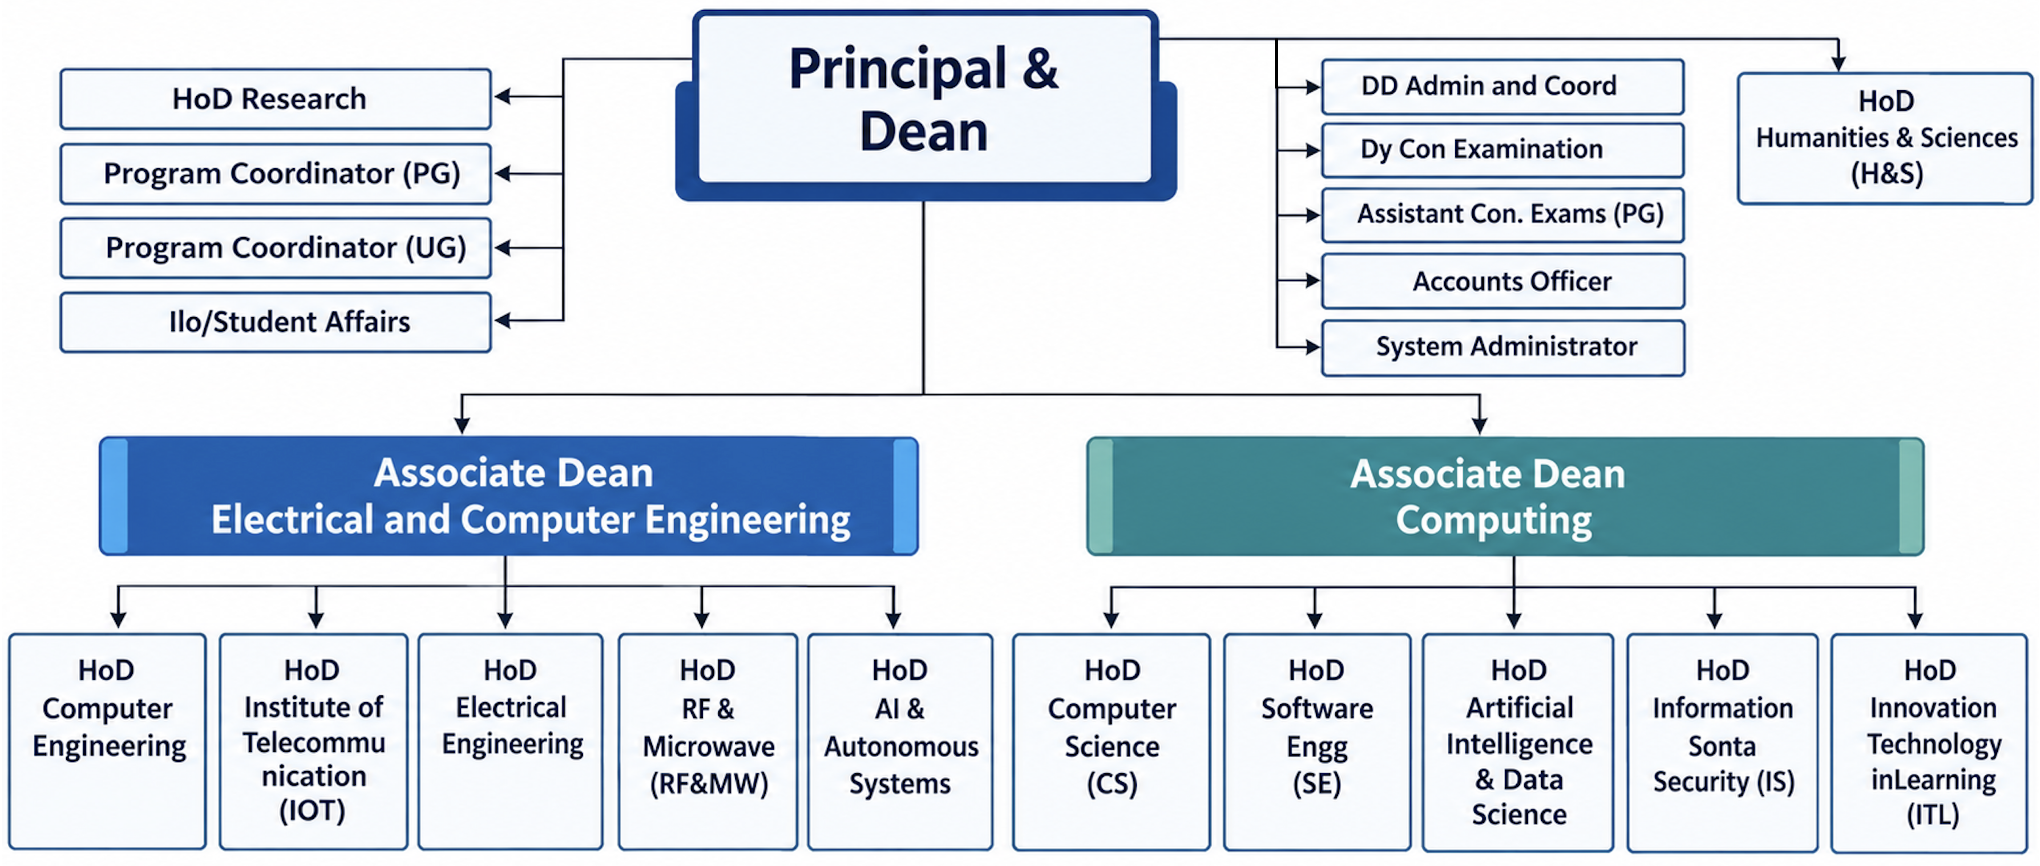
\includegraphics[width=1.0\textwidth]{images/front_matter/media/organogram.png}
    \caption{NUST-SEECS Organization}
    \label{fig:organ}
\end{figure}
\section{Accreditation History}\label{accreditation-history}

The BE Software Engineering program has undergone periodic accreditation and review by the Pakistan Engineering Council (PEC). Its accreditation history is summarized in Table~\ref{tab:history}.
\begingroup
\scriptsize
\setlength{\tabcolsep}{2pt}
\renewcommand{\arraystretch}{1.12}
\begin{longtable}{@{}>{\raggedright\arraybackslash}p{0.25\textwidth}>{\raggedright\arraybackslash}p{0.25\textwidth}>{\raggedright\arraybackslash}p{0.46\textwidth}@{}}
\caption{Accreditation History of BE Software Engineering Program}
\label{tab:history}\\
\toprule
\textbf{Date of Visit} & \textbf{Purpose} & \textbf{Remarks}\tabularnewline
\midrule
\endfirsthead
\toprule
\textbf{Date of Visit} & \textbf{Purpose} & \textbf{Remarks}\tabularnewline
\midrule
\endhead
\hline
September 2010 & Zero visit & Commencement of program approved\tabularnewline
\hline
24 June 2013 & Change of Scope & SEECS allowed to admit 2 sections\tabularnewline
\hline
18--19 June 2014 & Accreditation visit & Batch of 2010 accredited\tabularnewline
\hline
18--19 February 2016 & Accreditation visit & Batches of 2011 and 2012 
accredited\tabularnewline
\hline
22--24 February 2017 & Accreditation visit & Program accredited for two years (Batches 2013 and 2014)\tabularnewline
\hline
17--18 October 2018 & Accreditation visit & Program accredited for three years (Batches 2015, 2016, and 2017)\tabularnewline
\hline
14--15 March 2022 & Accreditation visit & Program accredited for two years (Batches 2018 and 2019)\tabularnewline
\hline
30--31 October 2023 & Accreditation visit & Program accredited for three years (Batches 2020, 2021, and 2022)\tabularnewline
\bottomrule
\end{longtable}
\endgroup

\section{Gap Analysis and Major Improvement Actions}\label{gap-analysis-for-implementation-of-obe-system}

The current review consolidates formal gaps recorded in the updated \emph{Gap Analysis} document and improvement needs addressed during the current accreditation cycle (Table~\ref{tab:gap-analysis-obe-current}). It distinguishes gaps identified through OBE review and previous PEC observations from subsequent program-level improvements documented in the 2026 SAR, reflecting progress beyond the initial 2014 OBE transition through PEC observations, internal CQI, Industrial Advisory Board (IAB) feedback, curriculum working papers, and institutional investment. These subsequent initiatives are presented as improvement needs, not new PEC deficiencies. Responses to previous PEC observations are consolidated in the \textbf{Rejoinder} under Criterion 8, while implementation evidence is provided under the relevant criteria and annexures to avoid duplication in Chapter 1.

\begingroup
\footnotesize
\setlength{\tabcolsep}{4pt}
\renewcommand{\arraystretch}{1.14}
\begin{longtable}{@{}>{\centering\arraybackslash}p{0.05\textwidth}>{\raggedright\arraybackslash}p{0.38\textwidth}>{\raggedright\arraybackslash}p{0.51\textwidth}@{}}
\caption{Expanded Gap Analysis and Major Improvement Actions}
\label{tab:gap-analysis-obe-current}\\
\toprule
\textbf{S. No.} & \textbf{Gap / Improvement Need} & \textbf{Action Taken / Current Status}\\
\midrule
\endfirsthead
\toprule
\textbf{S. No.} & \textbf{Gap / Improvement Need} & \textbf{Action Taken / Current Status}\\
\midrule
\endhead
\midrule
\multicolumn{3}{r}{\footnotesize\itshape Continued on next page}\\
\endfoot
\bottomrule
\endlastfoot

1 & The Alumni and Employer Survey
instruments required stronger and
more balanced alignment with the
Program Educational Objectives (PEOs) Key Performance Indicators
(KPIs). & The Alumni and Employer Surveys were redesigned in 2026 to strengthen alignment with PEO KPIs, each comprising 12 five-point Likert items, with four dedicated to each PEO. The instruments were approved by Department Board of Studies (DBS) on 20 April 2026 and Faculty Board of Studies (FBS) on 21 April 2026, and endorsed by IAB on 5 May 2026. Pilot normalized PEO scores were 0.803, 0.797, and 0.803, confirming attainment of all three PEOs. This addresses a previous PEC concern discussed in (Criteria 1 and 8 \& Rejoinder).\\
\addlinespace[2pt]
2 & The legacy PEO evaluation framework and follow-up mechanism required clearer, more traceable corrective-action logic. & A transparent multi-step PEO evaluation framework was introduced, covering question-level KPI checks, indicator coverage, and normalized PEO scoring. Corrective actions are tracked through a standard Corrective Action Form, ensuring an auditable CQI trail.\\
\addlinespace[2pt]
3 & The Graduate Exit Survey provided limited direct traceability between survey questions and individual Program Learning Outcomes (PLOs). & The Graduate Exit Survey was redesigned with each item mapped to a specific PLO and deployed through the Learning Management System (LMS), providing structured, PLO-wise indirect evidence for recent graduating batches (Criteria 2 and 8).\\
\addlinespace[2pt]
4 & Internship feedback provided insufficiently structured indirect PLO evidence and depended on a largely manual collection process. & The Internship Employer Feedback Form was redesigned with direct PLO mapping and integrated into the Online Internship Module. Combining employer feedback with faculty assessment provides traceable dual-source evaluation and addresses the previous PEC observation on indirect assessment (Criteria 2, 3, 8, and Rejoinder).\\
\addlinespace[2pt]
5 & The Software Engineering PLO framework required alignment with the revised PEC/HEC graduate attributes, which reduced the number of graduate attributes from 12 to 11. & The BESE PLO framework was revised from 12 to 11 to align with current PEC requirements, consolidating society and sustainability attributes within the revised graduate-attribute structure and updating the remaining PLOs. Batch-specific implementation and mapping are documented in Criterion 2 and the approved curriculum working papers.\\
\addlinespace[2pt]
6 & The curriculum required periodic regulatory alignment with successive PEC/HEC Undergraduate Education Policy updates and NUST academic requirements. & Three major curriculum working papers were processed: the 64th ACM (2023) redistributed FYDP credit hours; the 69th ACM (2024) incorporated UEP-2023 requirements, including the revised PLO structure and updated non-engineering courses requirements. Details are provided in Criterion 3; and the 72nd ACM (2025) incorporated UEP-2024 changes\\
\addlinespace[2pt]
7 & The program required broader field-specific elective choice and strengthening of the programming foundation. & Engineering electives were increased from five to six, with emerging offerings including Virtual and Augmented Reality, Introduction to Quantum Computing, Large Language Models, and Reinforcement Learning. Fundamentals of Computer Programming course credit hours were increased from 3 to 4 and Applications of ICT was introduced to strengthen computing/programming foundations of fresh intake. These changes reflect curriculum review and IAB recommendations (Criteria 3 and 9).\\
\addlinespace[2pt]
%8 & A formal academic mechanism for recognizing validated professional/certification-based learning was not available. & NUST Working Paper No. 2 of the 73rd ACM approved a framework for departmentally validated certification-style courses carrying 1--3 credit hours. The initiative has institutional approval but remains subject to the final PEC Engineering Accreditation Board SOP. \textbf{Status: Partially implemented / awaiting PEC SOP.}\\
%\addlinespace[2pt]
8 & Complex Engineering Problems (CEP) required a documented and consistently applied departmental mechanism across relevant courses. & A formal departmental CEP policy was documented and disseminated, requiring courses with laboratories/projects to incorporate relevant CEP elements addressing complex problem formulation, analysis, and solution development. Policy and implementation evidence are provided in Criterion 3.\\
\addlinespace[2pt]
9 & Open-Ended Laboratory (OEL) practice required more systematic institutionalization. & OEL activities were institutionalized in relevant laboratory courses, requiring students to develop methodologies, justify engineering decisions, and validate solutions beyond predefined procedures. Supporting policies and examples are provided in Criterion 3.\\
\addlinespace[2pt]
10 & Internship mechanism needed to be strengthened as a structured component of professional preparation and graduation requirements. & A 6–8-week internship is now mandatory for BESE graduation, supported by SEECS Industry Liaison Office (ILO) and NUST Placement Office (NPO) placement coordination. The LMS module enables digital feedback collection, complemented by employer and faculty evaluations (Criteria 3, 4, and 8).\\
\addlinespace[2pt]
11 & Faculty required continuing development in OBE implementation, particularly CLO formulation, Bloom's Taxonomy, PLO mapping, CEP and OEL. & 
Department-level OBE training is conducted at the start of each semester for all faculty, including new, continuing, and TVF members. Newly inducted faculty also receive mandatory one-week HR-led onboarding, with OBE training as a core module. Additional post-PEC sessions were conducted to strengthen faculty's taxonomy-level understanding. Institutional funding supports pedagogical training, certifications, and conference participation (Criteria 5, 7, and 8).\\
\addlinespace[2pt]
12 & Course outlines required comprehensive CLO--PLO mapping and explicit identification of appropriate teaching and assessment methods. & Course outlines and CLO–PLO mappings are periodically revised through faculty knowledge heads and CQI reviews. Each Course Learning Outcome (CLO) is linked to appropriate direct and/or rubric-based assessments, with course and laboratory folders maintained on the LMS for traceability and review.\\
\addlinespace[2pt]
13 & Some CLOs/courses were mapped at lower or inappropriate Bloom's Taxonomy levels, requiring stronger taxonomy alignment. & CLO wording and taxonomy levels are periodically reviewed and revised through course-level and departmental CQI processes.\\
\addlinespace[2pt]
14 & CQI actions required a more consistent institutional mechanism for ownership, documentation, follow-up and closure. & A dedicated CQI Committee reviews assessment results and monitors corrective actions. A standardized Corrective Action Form tracks actions, responsibilities, follow-up, and closure across curriculum, CLO, PLO, and PEO improvements, ensuring an auditable record (Criterion 8 and relevant annexures).\\
\addlinespace[2pt]
15 & OBE records and attainment analysis required sustainable digital documentation and reliable semester-/batch-wise reporting. & Course and laboratory folders are maintained on the LMS, while NUST’s Qalam OBE system generates semester- and batch-wise CLO/PLO attainment reports, strengthening record continuity, auditability, and data-driven CQI (Criteria 2, 3, and 8).\\
\addlinespace[2pt]
%17 & Students with weak individual PLO attainment required an explicit monitoring and recovery mechanism before graduation. & Individual PLO performance is monitored through Qalam. Students with identified deficiencies receive advisory or warning communication depending on stage of study, and additional/recovery learning is arranged where required. Full PLO attainment is checked as part of degree-completion monitoring. See Criteria 2 and 4.\\
%\addlinespace[2pt]
16 & SEECS had active industry collaboration, but a formal mechanism for recording and monitoring industry-sponsored FYDPs was missing. & TMS now records industry-sponsored FYDPs and co-supervision by SEECS faculty and industry/NSTP professionals, providing a formal digital audit trail. The platform also maintains internship evidence (Criteria 8 and 9).\\
%\addlinespace[2pt]
%19 & Industry input needed to translate more systematically into documented program and curriculum improvements. & The Industrial Advisory Board has met regularly during the accreditation cycle. The initiatives review records eight IAB sessions from May 2023 to May 2026, with 20 recommendations and 12 closed actions. Closed items include new electives, strengthening of programming credit hours and revision of PEO assessment instruments. See Criteria 1 and 9.\\
\addlinespace[2pt]
17 & Physical and computing infrastructure required expansion and modernization to support growing academic, laboratory and project needs. & The new SEECS Academic Block adds 14 classrooms, six teaching laboratories, three FYDP laboratories, faculty and officer offices, and supporting academic spaces. Computing facilities were further strengthened through the procurement of 45 new PCs and upgrades to 50 existing PCs.\\
\addlinespace[2pt]
18 & Network access and supporting digital/library infrastructure required continued strengthening for teaching, research and remote access. & SEECS has 910 Mbps PERN connectivity through the NUST campus core network, a 7 Mbps backup for research laboratories, and VPN-based remote access. Library facilities include high-speed internet, Wi-Fi, group study rooms, and academic spaces (Criteria 6 and 7).\\
\addlinespace[2pt]
19 & Student support made more integrated, accessible mechanisms covering administrative facilitation, counselling and employability. & NUST has introduced/strengthened centralized support through the Student Support Services Centre (S3C), the Centre for Counselling and Career Advisory (C3A), and the Career Development Centre (CDC). These provide one-window facilitation, professional counselling/career assessment, employability development and employer engagement. See Criteria 4, 6 and 9.\\
\end{longtable}
\endgroup

%\section{Historical Review of OBE Implementation}\label{historical-review-of-obe-implementation}

%SEECS initiated its formal transition to Outcome-Based Education (OBE) in June 2014 in response to the PEC Manual of Accreditation 2014. The first phase focused on defining and approving the program Mission, PEOs and PLOs, followed by faculty awareness and training on OBE principles, CLO--PLO mapping, Bloom's Taxonomy, course-outline design, teaching methods and assessment practices. These activities led to the adoption of OBE-aligned course outlines and assessment practices from Fall 2014 onward.

%The implementation was subsequently strengthened through continued faculty development, periodic accreditation reviews and the introduction of supporting academic systems. QOBE software was introduced in 2016 to facilitate management of outcome-based assessment data. Engagement with the Industrial Advisory Board and formal CQI meetings further supported review of curriculum relevance and attainment results. Workshops on emerging OBE practices continued, and newly inducted faculty were provided OBE orientation to maintain consistency in implementation.

%By 2021, OBE processes had become integrated with the institutional academic management framework through training on QALAM and routine use of the program's Quality Management System. The historical progression from initial OBE adoption to a structured CQI-based system established the foundation for the present assessment, review and corrective-action mechanisms described in the subsequent criteria of this SAR.

\section{Quality Management System}\label{quality-management-system}

The NUST Quality Management System (QMS) comprises various entities responsible for monitoring, managing, and enhancing academic quality in accordance with NUST statutes, policies, and associated addenda. The Software Engineering Department at SEECS has implemented an OBE-focused QMS (Figure~\ref{fig:qms}), operating through a hierarchical structure comprising the Local Quality Enhancement Cell (LQEC), Department Board of Studies (DBS), Faculty Board of Studies (FBS), University Curriculum Review Committee (UCRC), and Academic Council Meeting (ACM).
\begin{figure}[!hb]
\centering
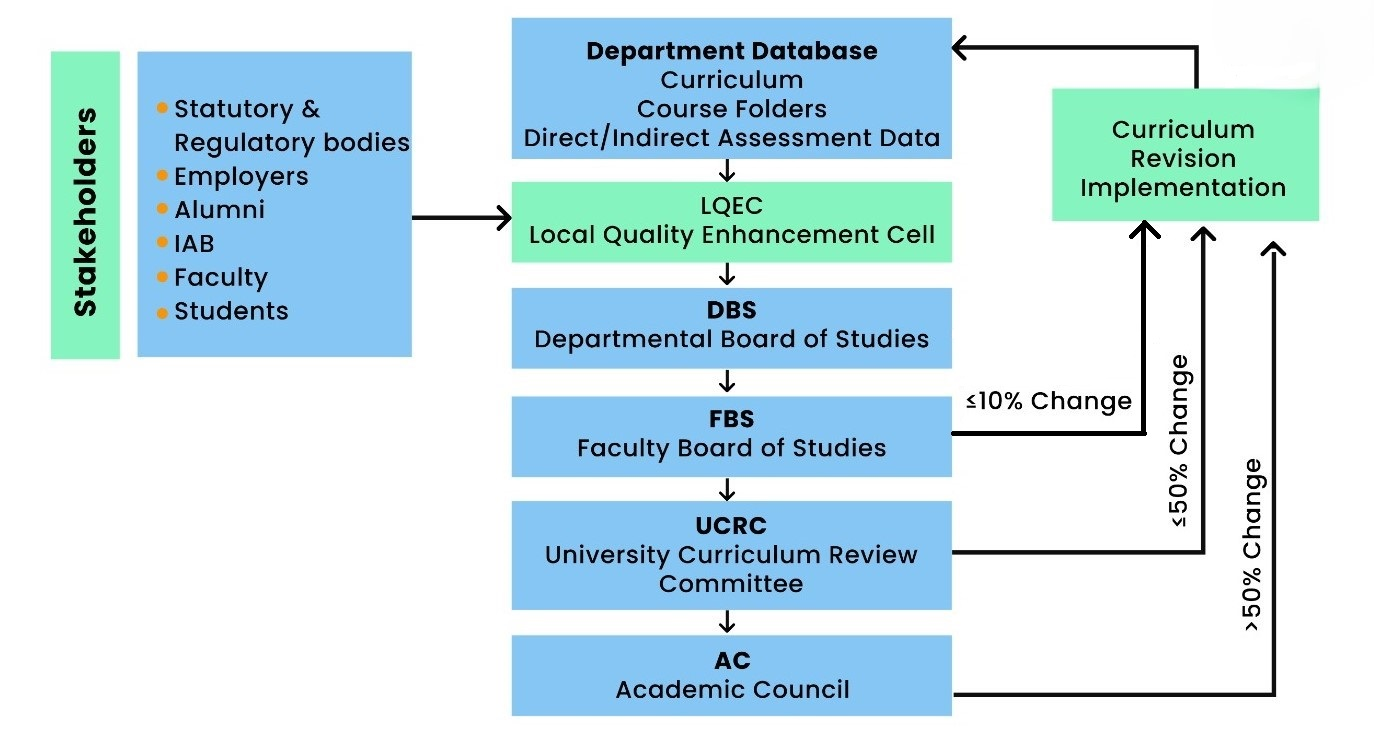
\includegraphics[width=1.0\textwidth]{images/criterion_8/media/Curr_review.jpeg}
\caption{Quality Management System (QMS)}
\label{fig:qms}
\end{figure}

\subsection{Local Quality Enhancement Cell (LQEC)}\label{local-quality-enhancement-cell}

Local Quality Enhancement Cell (LQEC) is composed of a nominated faculty member responsible for quality assurance of the program. It oversees the quality assessment process being carried out for the program. The LQEC is assisted by Knowledge Group Heads who make sure the course outline and exams are according to the guidelines. The primary role of LQEC is to analyze data collected from various sources such as exams/rubrics, various surveys and feedback. LQEC invokes corrective action process in case of deficiency observed because of CQI. Figure~\ref{fig:pqms} shows the flowchart for a typical CQI process for all levels of the program.

\begin{figure}[!hb]
\centering
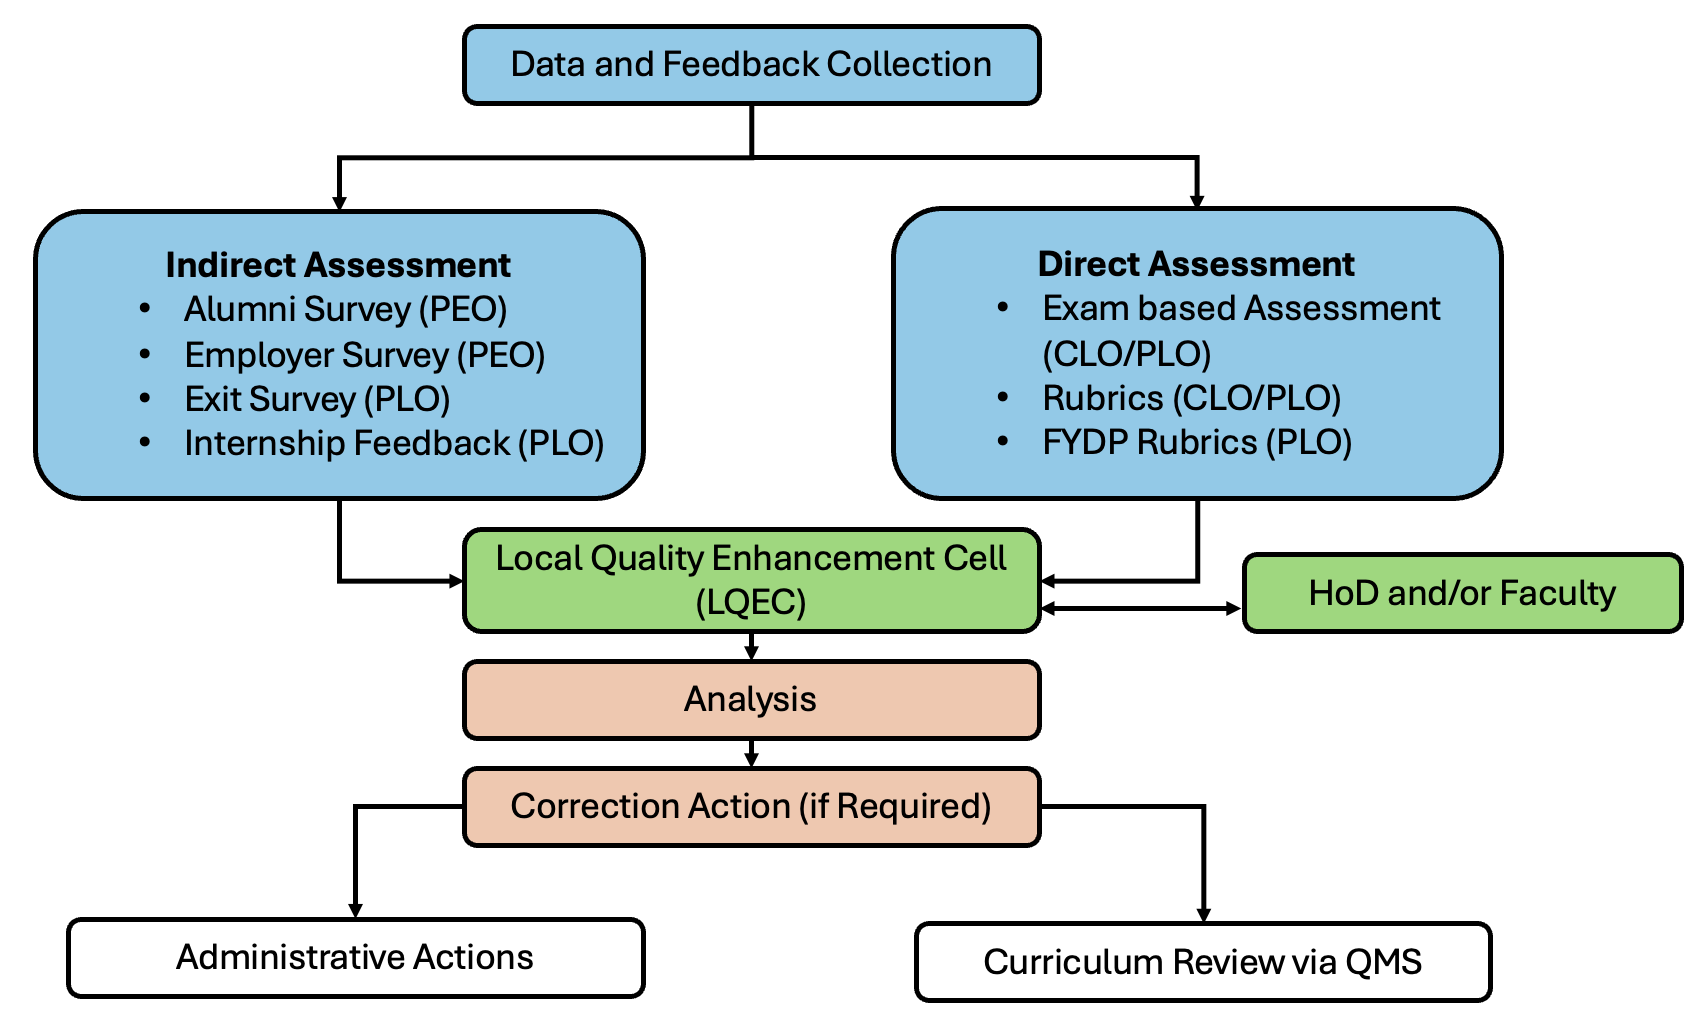
\includegraphics[width=1.0\textwidth]{images/front_matter/media/image-5.png}
\caption{Program Quality Assurance Process}
\label{fig:pqms}
\end{figure}

\subsection{Department Board of Studies}\label{department-board-of-studies}

Department Board of Studies (DBS) is composed of Associate Dean (Chairman), LQEC, all Heads of Departments (HoDs), program coordinator and assistant controller exams. The meeting is convened to present results, attainment of CLOs, PLOs and PEOs for different batches and to initiate any changes if required.

\subsection{Faculty Board of Studies}\label{faculty-board-of-studies}

Faculty Board of Studies (FBS) is composed of Principal SEECS, both Associate Deans of SEECS, all HoDs of SEECS, Deputy Controller Exams, and representatives from NUST main office. Any changes resulting from corrective actions in curricula up to 10\% are approved in FBS and implemented. More than 10\% of changes are approved for presentation in UCRC.

\subsection{University Curriculum Review Committee}\label{university-curriculum-review-committee}

University Curriculum Review Committee (UCRC) is composed of Pro Rector Academics (Chairman), Registrar, Director QA, Director PGP, Principal SEECS, Associate Dean Computing, Industrial Representatives, Director Research and Director Academics. Changes in curriculum up to 50\% are approved in UCRC. More than 50\% are approved for presentation in Academic Council Meeting.

\subsection{Academic Council}\label{academic-council}

Academic Council (AC) is composed of Rector NUST (Chairman), Pro Rector Academics, Pro Rector P\&R, Registrar, Principals or Deans of all Schools, Director QA, Directors of all NUST Directorates, and Industrial Representatives, as needed. Any major changes (more than 50\%) forwarded by UCRC are discussed and approved by Academic Council.

\section{Industry Advisory Board (IAB)}\label{industry-advisory-board-iab}

In addition to the several bodies discussed above, SEECS holds regular meetings of the board of industry representatives and alumni. This board provides a formal platform for interaction with industrial experts and alumni to provide feedback about the program, its direction, curriculum, and any other related matters.

\section{Corporate Advisory Council (CAC)}\label{corporate-advisory-council-cac}

The CAC was formed in 2010 under chairmanship of Rector to create a positive impact on the socio-economic development of Pakistan through active engagement with the industry. The CAC has been instrumental in developing linkages with industrial and business enterprises across multiple sectors of the economy.

%\paragraph{Facilities and safety evidence.} Detailed information on institutional facilities, workplace safety, fire-safety arrangements, and supporting evidence is presented under Criterion 6 and is not duplicated in the Introduction.

\section{OBE Implementation Model}\label{obe-implementation-model}

The OBE implementation model is a continuous process in which the attainment of the Program Mission and PEOs is monitored through indirect assessments. SEECS formally initiated OBE implementation in June 2014 in response to the PEC Manual of Accreditation 2014, followed by faculty training and the adoption of OBE-aligned course outlines and assessment practices. Implementation was strengthened through continued faculty development, the introduction of QOBE software in 2016, engagement with the Industrial Advisory Board (IAB), and formal Continuous Quality Improvement (CQI) reviews. By 2021, OBE processes had been integrated into academic management through QALAM training and the routine use of the program's Quality Management System. The flowchart in Figure~\ref{review of PEOs} illustrates the CQI process through three interconnected loops: the outermost loop monitors PEO attainment and overall program success, the middle loop assesses PLO attainment, and the innermost loop evaluates CLO attainment. Each loop follows four steps i.e. data collection, evaluation, review, and corrective action.
\begin{figure}[H]
\centering
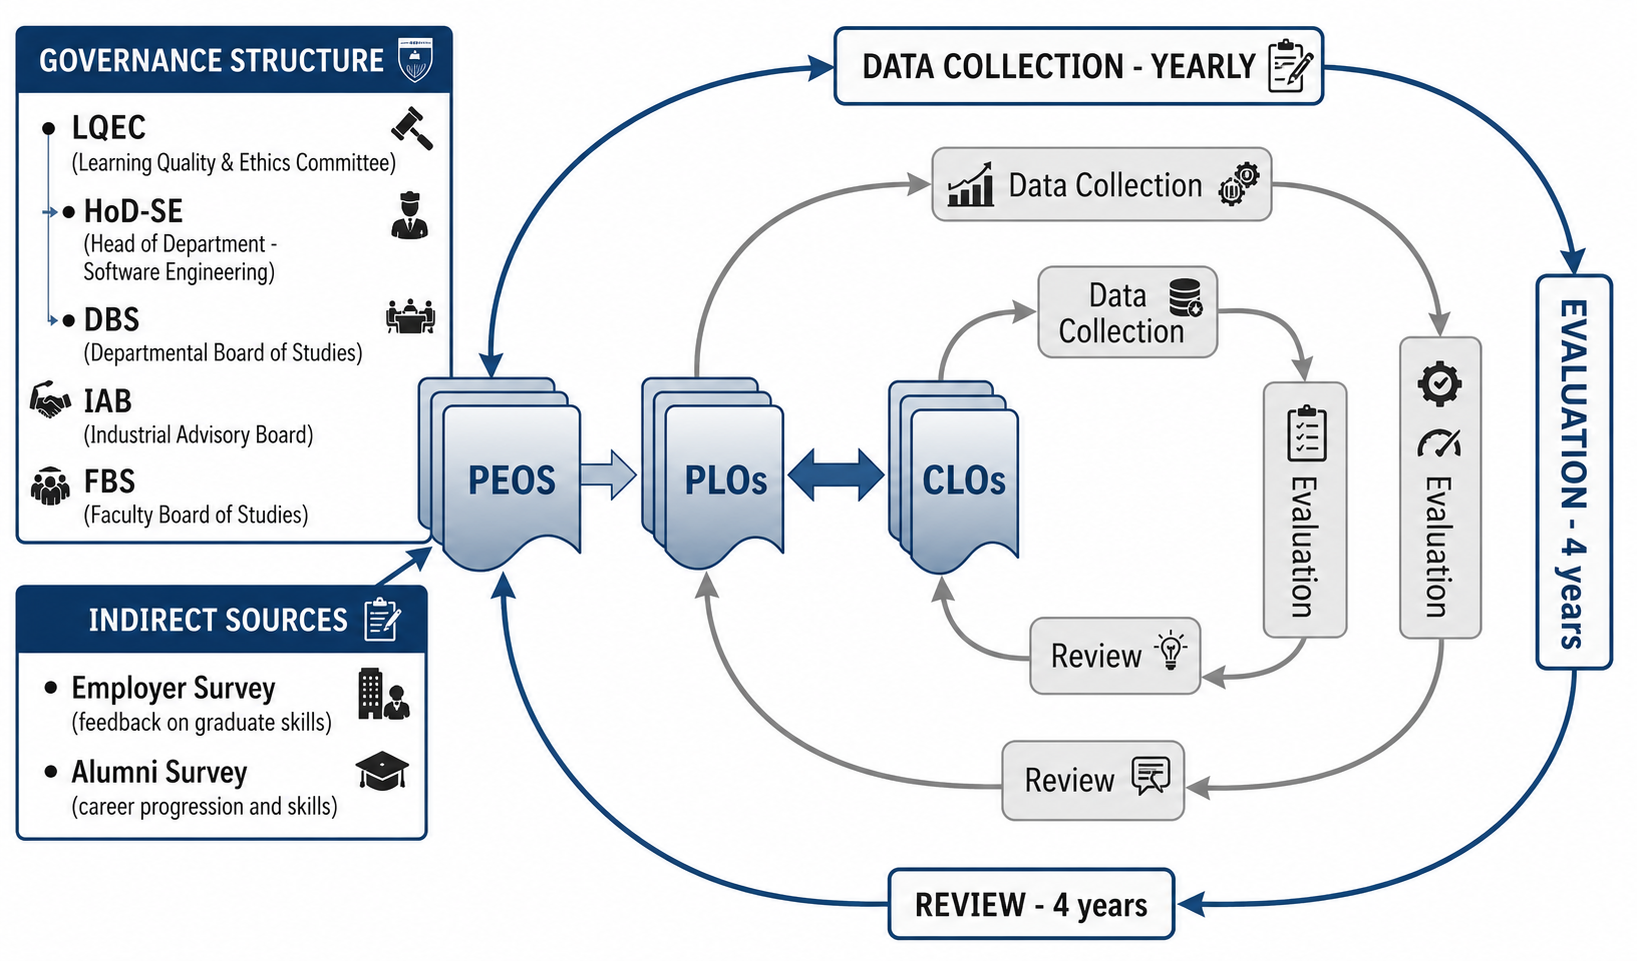
\includegraphics[width=1.0\textwidth]{images/front_matter/media/image13.png}
\caption{CQI Process through Three Interconnected Loops}
\label{review of PEOs}
\end{figure}
\subsection{CQI Process for PEOs}\label{peos}
%\subsubsection{CQI Process for PEOs}\label{cqi-process-for-peos}

The LQEC is responsible for the initiation of CQI for attainment, revision, and improvement of PEOs. PEOs are indirectly assessed through alumni and employer surveys, with data collected yearly and review carried out four years after graduation of each batch. The review process starts with measurement of PEOs and involves CQI, corrective actions and administrative processes for maintenance and/or improvement of PEOs as shown in Figure~\ref{fig:corrective action processes for PEOs}. If the achievement of PEOs is attained, no corrective action is required; otherwise, the CQI process is invoked by LQEC.

\begin{figure}[H]
\centering
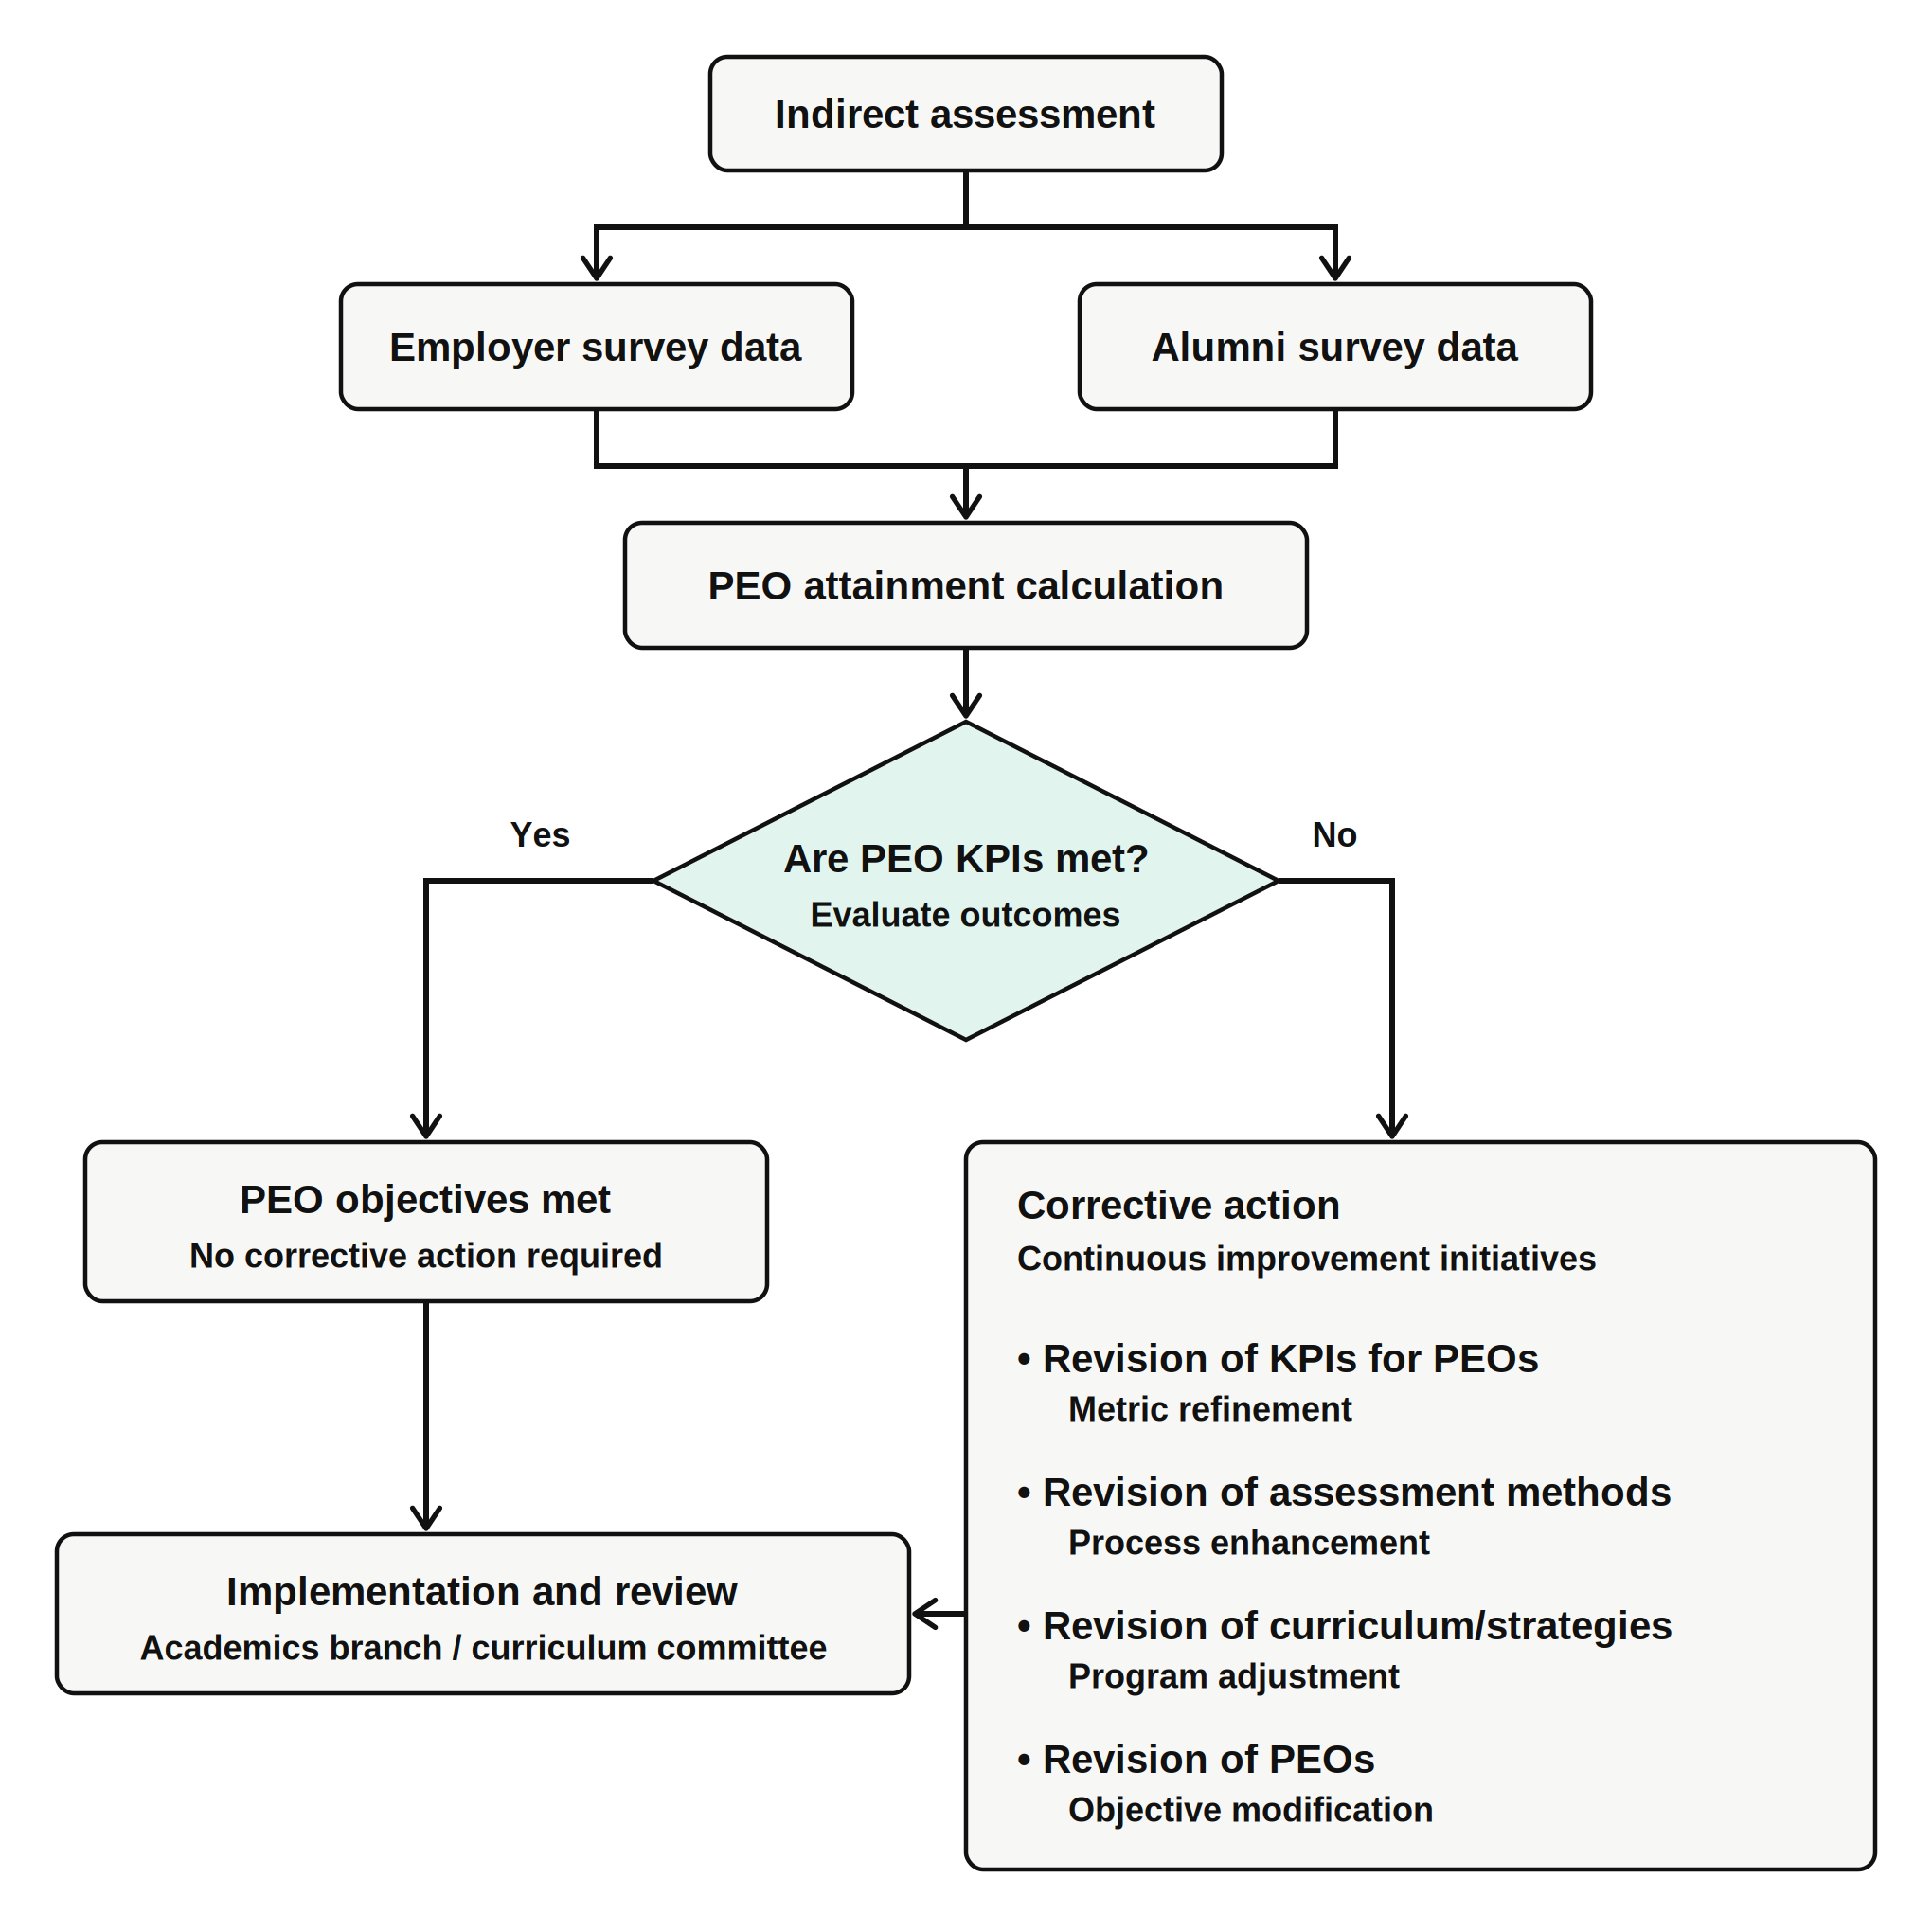
\includegraphics[width=0.89\textwidth]{images/front_matter/media/image-14.png}
\caption{Flowchart Showing Review \& Corrective Action Processes for PEOs}
\label{fig:corrective action processes for PEOs}
\end{figure}
%\subsubsection{Review and Corrective Action Processes for PEOs}\label{review-and-corrective-action-processes-for-peos}

\subsection{CQI Process for PLOs}\label{plos}

%\subsubsection{CQI Process for PLOs}\label{cqi-process-for-plos}

LQEC is responsible for CQI process for evaluation and attainment of PLOs. PLOs are directly assessed through CLOs and Final Year Design Projects (FYDPs), whereas indirect assessment is done through internship feedback and exit surveys (Figure~\ref{fig:corrective action processes for plos}).  Figure~\ref{fig:individual-level1} and Figure~\ref{fig:cohort level}, show the review process for PLOs at individual and cohort levels respectively. Individual PLO analysis starts with direct assessment, where each student’s PLO attainment is calculated in their courses and then analysed against the respective KPI. If the KPI is met, no corrective action is needed. If the KPI is not met, the student moves through escalating stages. A counselling stage with a letter of advice comes after semesters 4–6. A warning stage with a warning letter comes after semester 7. If attainment is still short after semester 8, the special module stage applies, with another warning letter and the department arranging extra module(s) to help the student reach the PLO. 

\begin{figure}[H]
\centering
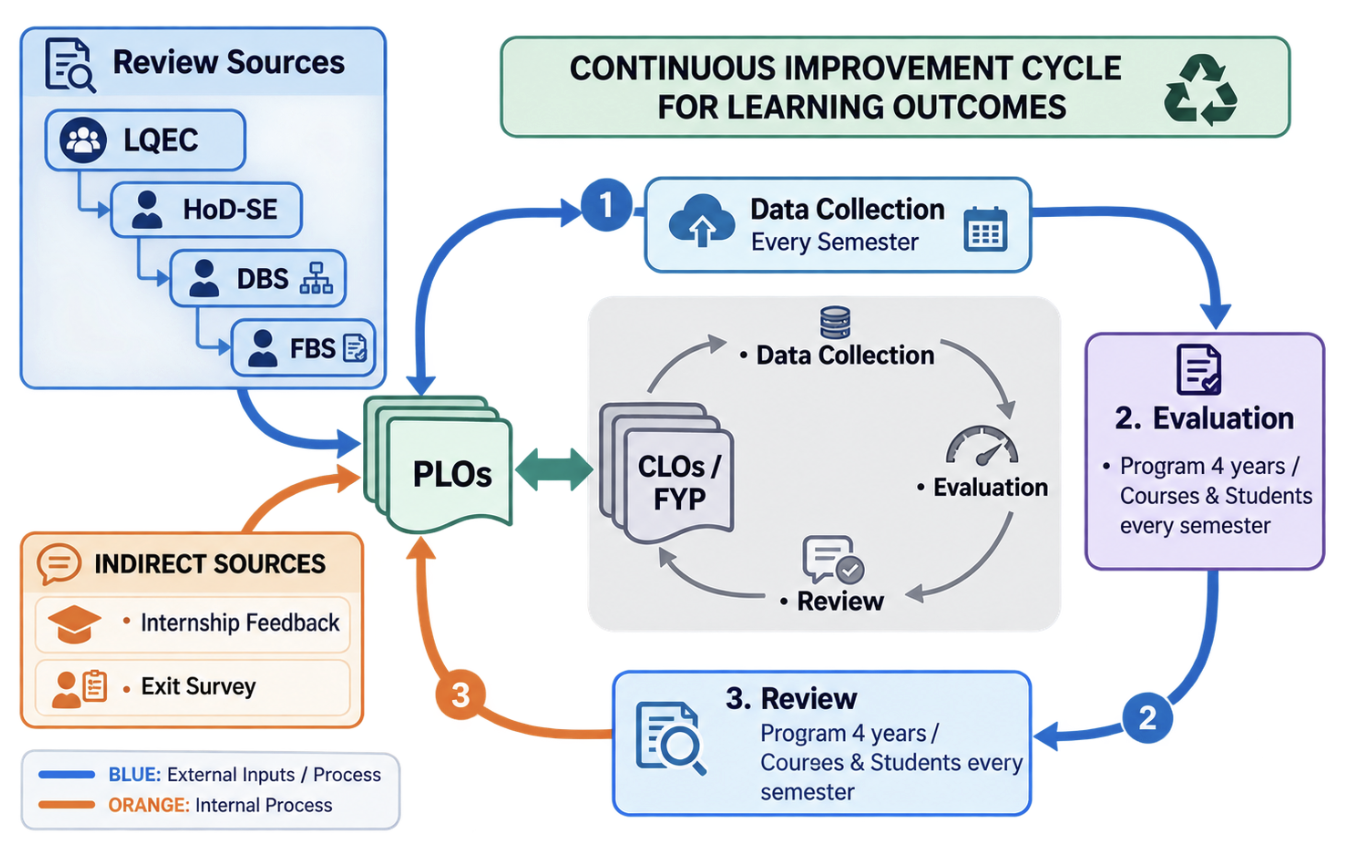
\includegraphics[width=0.88\textwidth]{images/front_matter/media/image-15.png}
\caption{Flowchart Showing Review \& Corrective Action Processes for PLOs}
\label{fig:corrective action processes for plos}
\end{figure}

For a cohort, if PLO attainment is more than or equal to 60\% as per KPI, no corrective action is required. Otherwise the CQI process invokes corrective actions including the revision of KPIs, CLO-PLO remapping, curriculum revision, and review of teaching \& learning processes.

%\subsubsection{Review and Corrective Action Processes for PLOs}\label{review-and-corrective-action-processes-for-plos}

\begin{figure}[H]
\centering
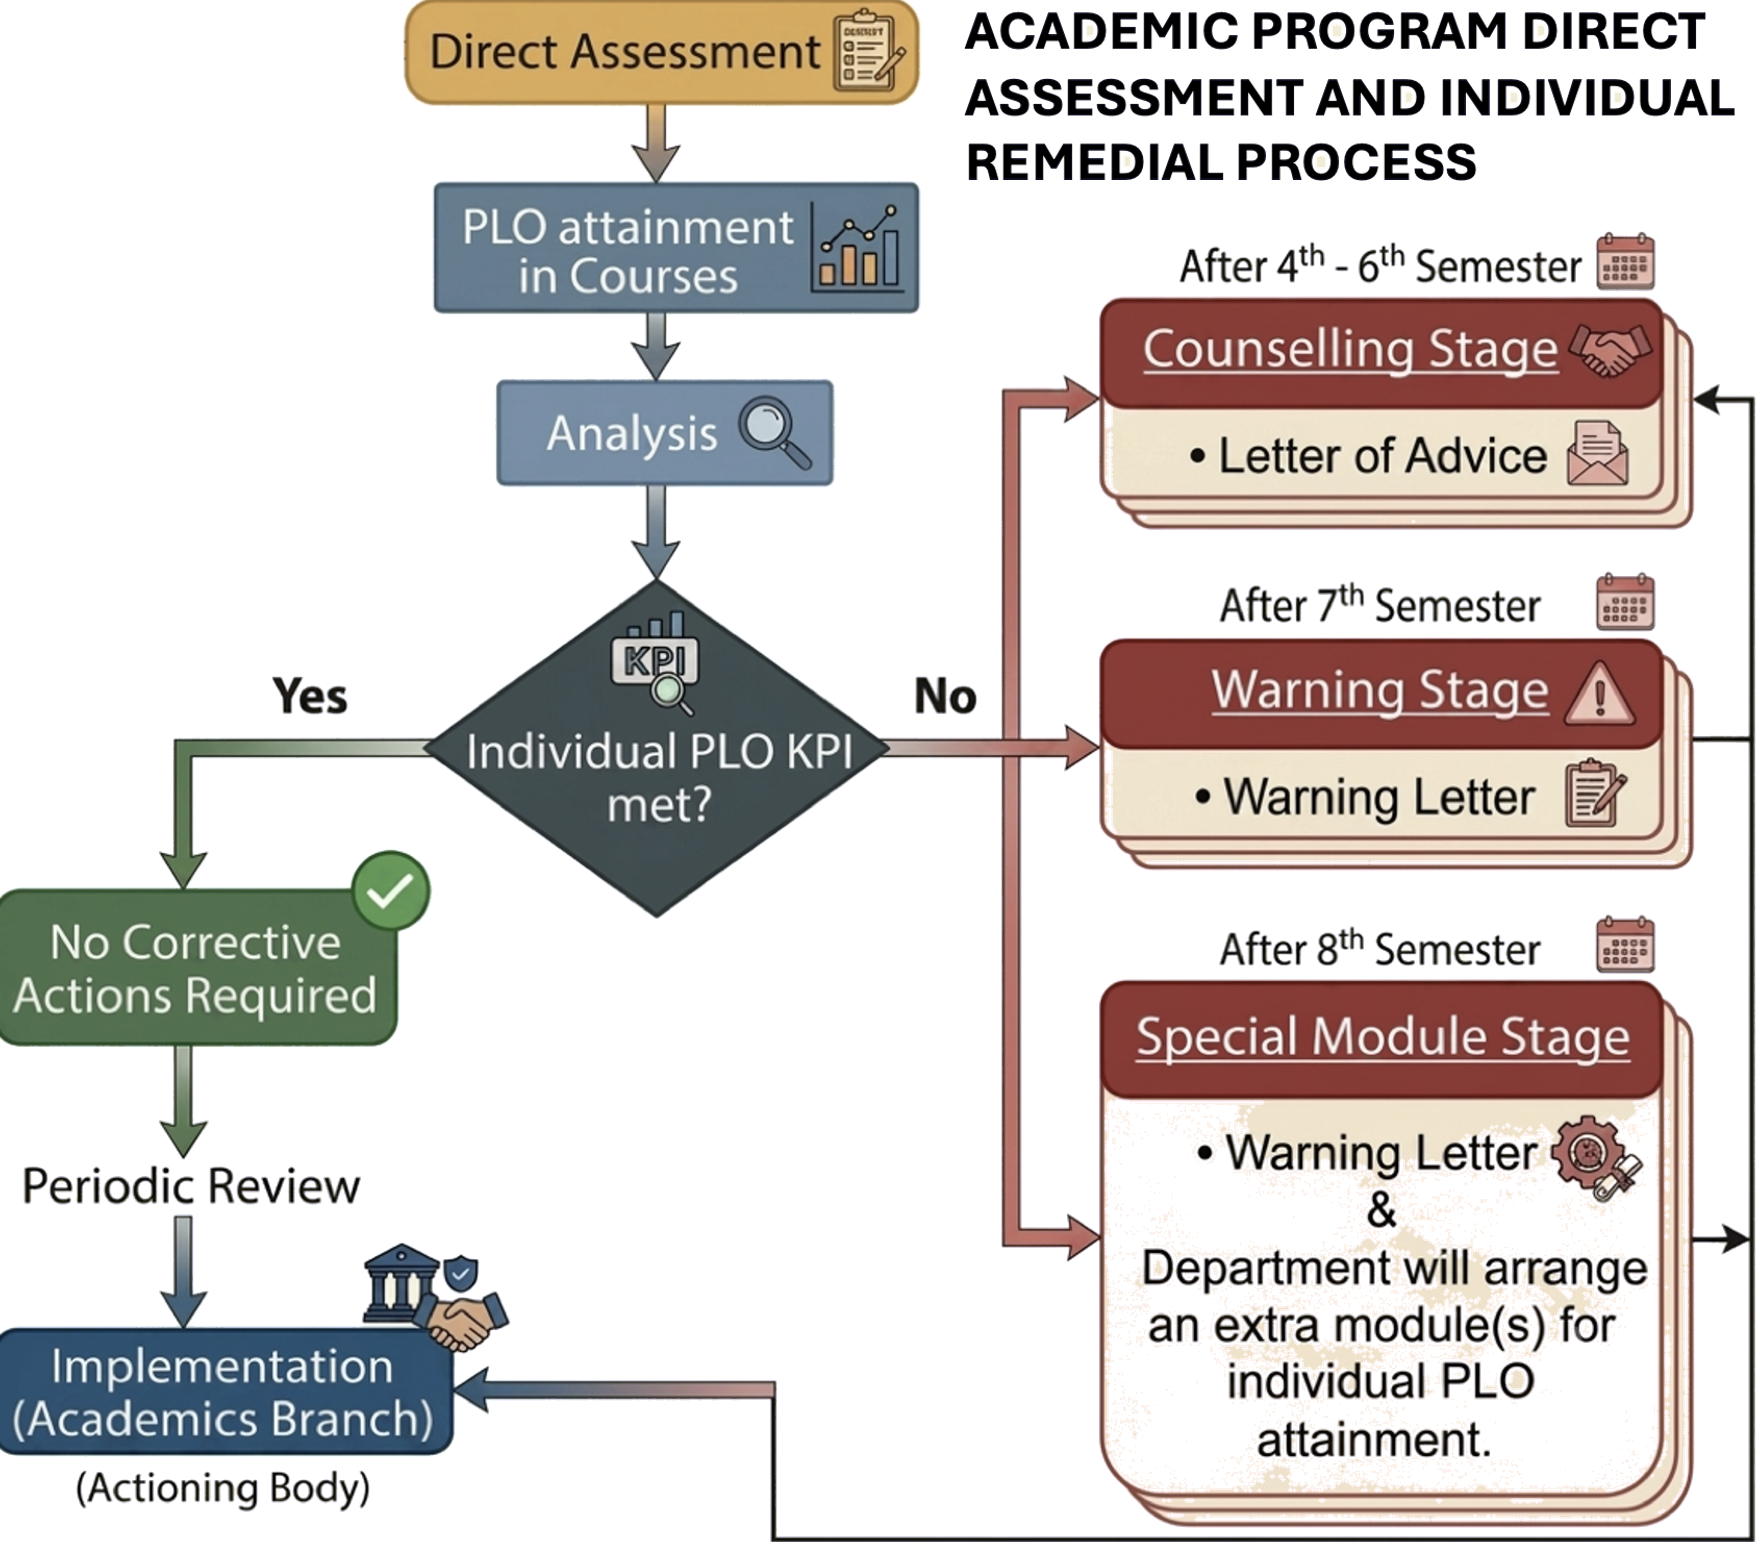
\includegraphics[width=0.7\textwidth]{images/front_matter/media/image-16.png}
\caption{Review of PLOs at Individual Level \& Corrective Actions}
\label{fig:individual-level1}
\end{figure}

\begin{figure}[H]
\centering
\includegraphics[width=0.8\textwidth]{images/front_matter/media/image17.png}
\caption{Review of PLOs at Cohort Level \& Corrective Actions}
\label{fig:cohort level}
\end{figure}

\subsection{CQI Process for CLOs}\label{clos}

%\subsubsection{CQI Process for CLOs}\label{cqi-process-for-clos}
The innermost loop of OBE implementation model deals with CQI process for CLOs (coursework) as shown in Figure~\ref{fig:cqi clo}. 
\begin{figure}[H]
\centering
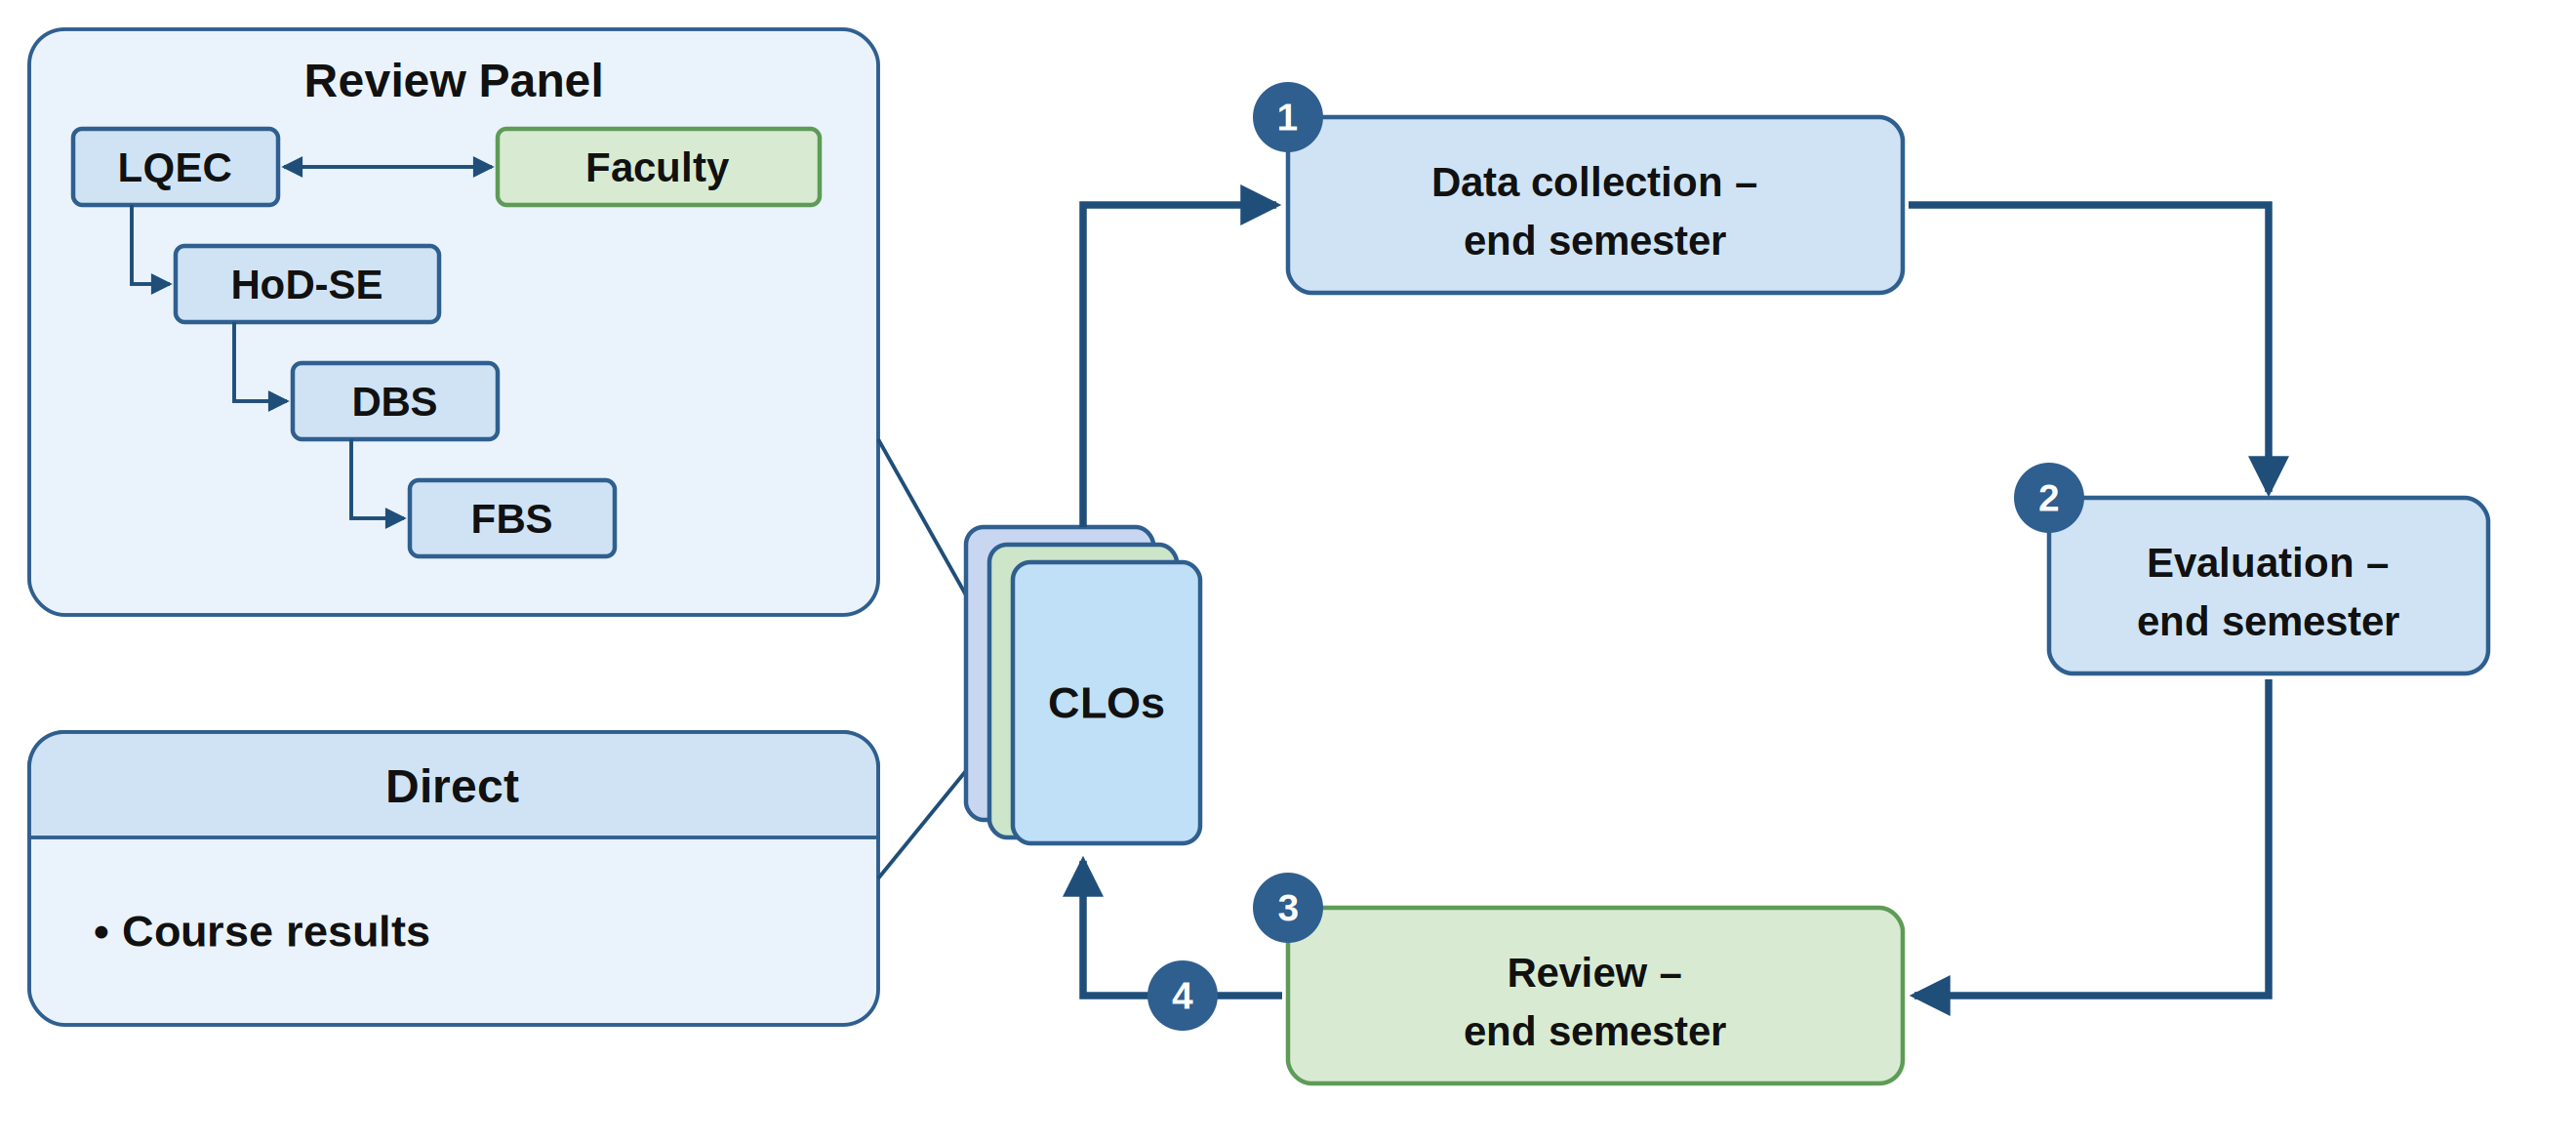
\includegraphics[width=1.0\textwidth]{images/front_matter/media/image-18.png}
\caption{Attainment and Review Process of CLOs}
\label{fig:cqi clo}
\end{figure}

CLOs are directly assessed through coursework and laboratory work involving examination and rubrics. For each course, the review process for attainment of CLOs is shown in Figure~\ref{fig:corrective CLOs}. If the cohort attainment of CLOs is equal to or more than 60\%, no corrective action is required. If cohort CLO attainment is less than 60\%, the corrective actions are invoked by the LQEC in consultation with the relevant faculty.
%\subsubsection{Review and Corrective Action Processes for CLOs}\label{review-and-corrective-action-processes-for-clos}

\begin{figure}[H]
\centering
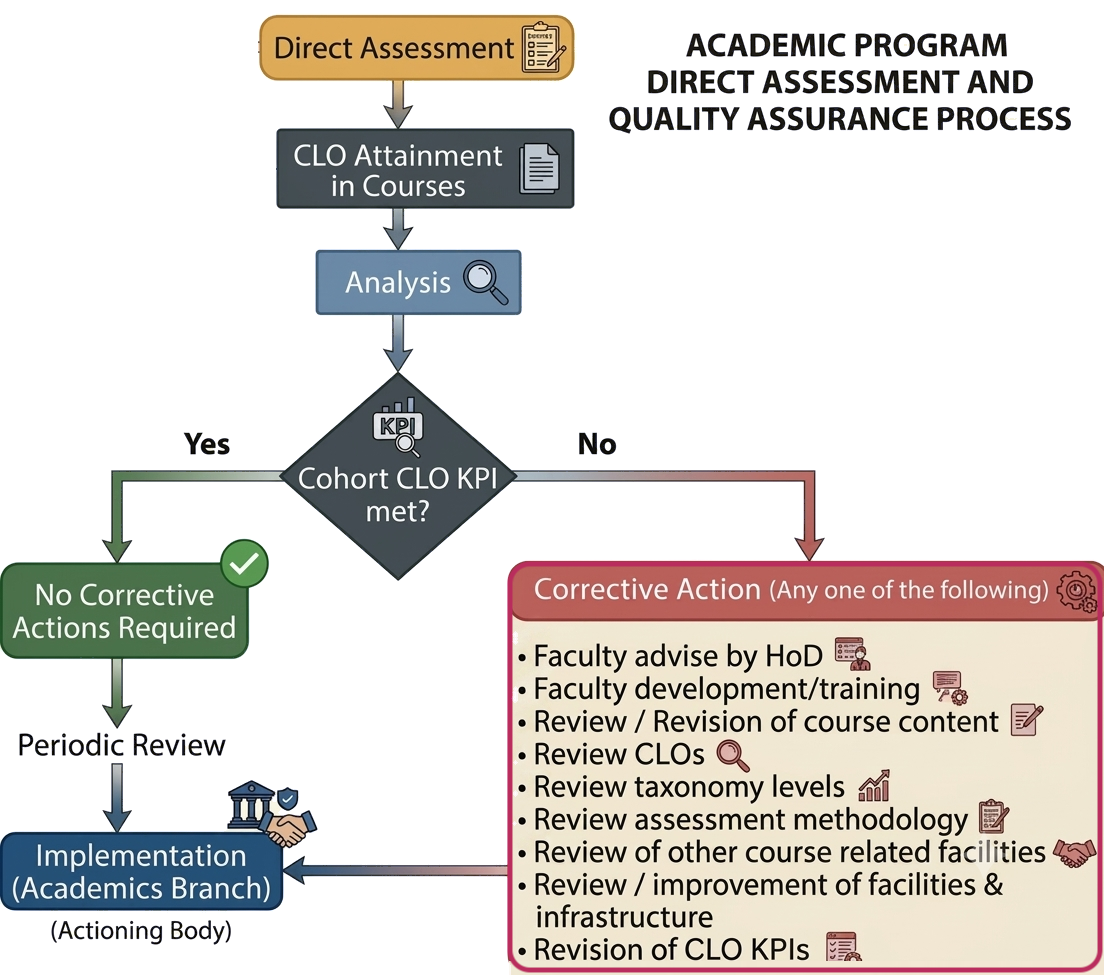
\includegraphics[width=5.18in,height=4.89in]{images/front_matter/media/image-19.png}
\caption{Corrective Actions for CLOs}
\label{fig:corrective CLOs}
\end{figure}

\section{Progress Since Last Accreditation Visit}\label{progress-on-last-accreditation-visit}

The previous PEC accreditation visit identified improvement opportunities across PEO assessment, PEO--PLO alignment, CLO/PLO mapping and taxonomy, indirect and direct assessment, and implementation of corrective actions. These observations have been addressed through the program's CQI mechanism. The complete institutional response to the previous visit is retained as Rejoinder under Criteria 8. The implementation status is discussed in Chapter~\ref{criterion-8-continual-quality-improvement} under Section~\ref{Implementation-Status-of-Previous-Accreditation-Observations}. To avoid duplicating the full rejoinder, Table~\ref{tab:last-visit-summary} summarizes the main action areas and points to the same supporting annexures used in Chapter~\ref{criterion-8-continual-quality-improvement}.

\begingroup
\footnotesize
\setlength{\tabcolsep}{4pt}
\renewcommand{\arraystretch}{1.15}
\begin{longtable}{@{}>{\raggedright\arraybackslash}p{0.24\textwidth}>{\raggedright\arraybackslash}p{0.48\textwidth}>{\raggedright\arraybackslash}p{0.20\textwidth}@{}}
\caption{Summary of Major Actions Following the Previous PEC Accreditation Visit}
\label{tab:last-visit-summary}\\
\toprule
\textbf{Area} & \textbf{Implemented Response} & \textbf{Supporting Evidence}\\
\midrule
\endfirsthead
\toprule
\textbf{Area} & \textbf{Implemented Response} & \textbf{Supporting Evidence}\\
\midrule
\endhead
\bottomrule
\endlastfoot
PEO assessment & Alumni and employer survey instruments were revised to improve question-to-PEO traceability and balanced coverage of the PEOs. & Chapter~\ref{criterion-1-program-educational-objectives}; Annexure A \\ %Annexure~\ref{revised-alumni-survey}; Annexure~\ref{revised-employ-survey}\\

\addlinespace[2pt]
PEO--PLO alignment & The PEO--PLO mapping was reviewed and updated, including explicit representation of innovation-related outcomes. & Chapter~\ref{criterion2}; Annexure B\\
%Chapter~\ref{sec:plopeo};Annexure~\ref{app:criteria-2_plo-peo_mapping_rationale}\\
\addlinespace[2pt]
CLO/PLO mapping and taxonomy & CLO wording, learning domains, Bloom's Taxonomy levels, and CLO--PLO mappings were reviewed through course and departmental CQI processes. &  Chapter~\ref{criterion2}\\
%Chapter~\ref{sec:cloplo}\\
\addlinespace[2pt]
Assessment and internship feedback & Direct-assessment practices and indirect assessment instruments, including internship feedback, were revised to strengthen outcome traceability and consistency. & Chapter~\ref{criterion2}; Chapter~\ref{criterion3}; Annexure B\\
%Chapter~\ref{sec:directassess}; Chapter~\ref{sec:indirectassess}; Chapter~\ref{sec:4.8internship}; Annexure~\ref{annex:internship-feedback-form}; Annexure~\ref{annex:graduate-exit-survey-form}\\
\addlinespace[2pt]
Corrective-action tracking & Corrective actions are documented and monitored through the formal CQI mechanism using Corrective Action Forms and follow-up review. & Chapter~\ref{criterion-8-continual-quality-improvement}\\
\addlinespace[2pt]
Curriculum response & Curriculum revisions arising from regulatory, assessment, and stakeholder inputs are processed through the approved academic governance mechanism. & Chapter~\ref{criterion3}\\
\end{longtable}
\endgroup


\clearpage

% ============================================================
% CHAPTER 2 — Criterion 1: Program Educational Objectives
% Images: images/criterion_1/media/
% ============================================================
\graphicspath{{images/criterion_1/media/}}
% --- Safety guard: define \arraybackslash if the array package failed to (e.g. broken MiKTeX install) ---
\makeatletter
\providecommand{\arraybackslash}{\let\\\@arraycr}
\makeatother
% ---------------------------------------------------------------------------------------------------
\chapter{Criterion 1: Program Educational Objectives (PEOs)}\label{criterion-1-program-educational-objectives}

Program Educational Objectives (PEOs) are the attributes and abilities that the graduates are expected to demonstrate within a few years of graduation, translated directly from the program's vision and mission and aligned with those of the University and School. Figure~\ref{fig:peo_process} gives an overview of the PEO development, evaluation, and continuous improvement process followed by the Software Engineering (SE) program at NUST-SEECS. The process incorporates input from internal stakeholders, including faculty and senior management, and external stakeholders, particularly industry representatives through the Industrial Advisory Board (IAB), while considering the requirements of relevant regulatory bodies, including PEC and HEC. PEO attainment is assessed via Alumni and Employer surveys, and the results feed into the CQI process governing subsequent revisions of PEOs, program's courses and teaching methodology.

\begin{figure}[tb]
\centering
\includegraphics[width=0.9\textwidth]{images/criterion_1/media/peo-evaluation.png}
\caption{PEO Development, Evaluation, and Continuous Improvement Process}
\label{fig:peo_process}
\end{figure}

%This chapter presents the vision and mission of NUST, SEECS, and the SE Department (Section~\ref{vision-mission}), the formulation, publication, and alignment of the SE program's PEOs (Section~\ref{peo-se}), the legacy and revised (2026) PEO attainment evaluation mechanisms (Section~\ref{attainment-of-peos}) and their results (Section~\ref{attainment-results}), and how these PEO attainment results drive continuous improvement of the program supplemented by the stakeholder (industry) feedback (Section~\ref{program-improvement}).

\hypertarget{vision-mission}{%
\section{Vision \& Mission of the University, School, \& Department}\label{vision-mission}}

The vision and mission statements of NUST\footnote{https://nust.edu.pk/about-us/visionandmission/}, SEECS\footnote{https://seecs.nust.edu.pk/about-us/vision-mission/}, and the SE Department\footnote{https://seecs.nust.edu.pk/departments/department-of-software-engineering/} provide the foundational reference points against which the program's PEOs are formulated and periodically reviewed. The NUST vision and mission statements are published on the university's official website, in the university prospectus and student handbook, and on display boards across the university. The SEECS and SE Department vision and mission statements are published on their respective official websites and displayed on boards within the department. The statements are presented below in hierarchical order, from the university level to the department level.

\begin{description}[leftmargin=1.6em,style=sameline,itemsep=5pt,topsep=4pt]
\item[NUST Vision:] NUST aspires to be a comprehensive university providing a higher education experience grounded in thought leadership, co-creation of knowledge, and sustainability.
\item[NUST Mission:] NUST is committed to being a university that stimulates intellectual curiosity, behavioral progression, and environmental stewardship. We nurture future leaders, job creators, and lifelong learners, with the ability to foster partnerships, and intercultural competence to impact their communities and beyond. Through adherence to our core values, we create an ecosystem that promotes research, innovation, and productivity.
\item[SEECS Vision:] To be a center of excellence for imparting high-quality education, promoting cutting-edge research and cultivating entrepreneurial culture, while instilling sound humanitarian values thus, contributing towards the knowledge economy of Pakistan.
\item[SEECS Mission:] In pursuance to NUST's vision, SEECS strives:
\begin{itemize}[leftmargin=1.3em,nosep,topsep=3pt]
\item To provide world-class education in the fields of Electrical Engineering and Computing through dedicated faculty, continuous quality improvement and a fair and conducive environment.
\item To promote progressive research through engagement with industry, government, and international collaborators.
\item To instill the spirit of humanity through awareness of social issues and participation in co/extra-curricular activities and community service.
\item To contribute to the development and economic progress of Pakistan by promoting the culture of entrepreneurship and enhancing leadership skills.
\end{itemize}
\item[Department Vision:] To become a world class Software Engineering program, focused on quality teaching, research and entrepreneurship in order to have a positive impact on society.
\item[Department Mission:] To prepare Software Engineering graduates having a concrete knowledgebase, sound analytical skills, and professional attitude through an enabling environment to undertake real world engineering problems, innovative research, and entrepreneurship, thus contributing to the society.
\end{description}

\hypertarget{peo-se}{%
\section{PEOs: Software Engineering Program at SEECS}\label{peo-se}}

\subsection{Formulation, Improvement, and Approval of PEOs} \label{sec:peo_process} 

The Software Engineering PEOs at NUST-SEECS are formulated based on desired graduate attributes, stakeholder input, and alignment with the vision and mission of NUST, SEECS, and the SE Department. As shown in Figure~\ref{fig:peo_process}, the PEOs undergo review by the LQEC, endorsement by the Head of Department (HoD-SE), review and approval by DBS, external feedback and endorsement by the IAB, and final ratification by the FBS. Stakeholder feedback informs both the formulation and periodic review of the PEOs. The process draws on faculty reviews, IAB recommendations, and Alumni and Employer survey evidence described in Section~\ref{attainment-of-peos}. This input enables the department to assess the continuing relevance of the PEOs against graduate attributes, professional expectations, and institutional priorities. The department collects indirect assessment data from Alumni and Employer surveys annually, evaluates PEO attainment on a four-year cycle (Section~\ref{attainment-of-peos}), and reviews the PEO statements every four years against assessment evidence, stakeholder input, and the vision and mission of NUST, SEECS, and the SE Department. The review determines whether revisions are required. This periodic review cycle has not yet been completed under the current PEOs and represents the department's planned practice going forward.

\subsection{PEOs and Their Publication} \label{sec:peo_publication} The approved PEOs of the SE program are as follows: 
\begin{enumerate} 
\item \textbf{Demonstrate sound~software~engineering knowledge~and~skill set.} 
\item \textbf{Lead diverse teams and work collaboratively to develop innovative solutions. }
\item \textbf{Conduct~professional practice~for sustainable development with due consideration for~societal, ethical, and environmental aspects.} 
\end{enumerate} 
The PEOs are published on the SEECS website\footnote{https://seecs.nust.edu.pk/department-page/obe-peo-plo/} and are also available through the prospectus and departmental display materials.

\subsection{PEO Consistency with Vision, Mission, \& Stakeholder Requirements} \label{consistency-of-peos}
The PEOs are aligned with the vision and mission of NUST, SEECS, and the SE Department, as well as the requirements of key stakeholders. Table~\ref{tab:peo_mapping} maps each PEO against the applicable vision and mission statements at each institutional level. A $\checkmark$ indicates direct, substantive alignment, while $\sim$ denotes partial or indirect alignment. PEO~2, which focuses on teamwork and collaborative leadership, is marked as partially aligned where these attributes are not explicitly reflected in the relevant vision and mission statements.

%\begin{landscape}
\begingroup
\footnotesize
\setlength{\tabcolsep}{5pt}
\renewcommand{\arraystretch}{1.15}
\begin{longtable}{@{}>{\centering\arraybackslash}p{0.03\textheight} >{\raggedright\arraybackslash}p{0.10\textheight} >{\raggedright\arraybackslash}p{0.37\textheight} >{\centering\arraybackslash}p{0.020\textheight} >{\centering\arraybackslash}p{0.020\textheight} >{\centering\arraybackslash}p{0.020\textheight}@{}}
\caption{PEOs Alignment to NUST, SEECS, \& Department's Vision \& Mission. (\checkmark = strong; $\sim$ = partial).}\label{tab:peo_mapping}\\
\toprule
\textbf{S. No.} & \textbf{Vision \& Mission} & \multicolumn{1}{c}{\textbf{Description}} & \multicolumn{3}{c@{}}{\textbf{PEOs}} \\
\cmidrule(l){4-6}
 & & & \textbf{1} & \textbf{2} & \textbf{3} \\
\midrule
\endfirsthead
\toprule
\textbf{S. No.} & \textbf{Vision \& Mission} & \multicolumn{1}{c}{\textbf{Description}} & \multicolumn{3}{c@{}}{\textbf{PEOs}} \\
\cmidrule(l){4-6}
 & & & \textbf{1} & \textbf{2} & \textbf{3} \\
\midrule
\endhead
\midrule
\multicolumn{6}{r}{\footnotesize\itshape Continued on next page}\\
\endfoot
\bottomrule
\endlastfoot
1 & NUST Vision & NUST aspires to be a comprehensive university providing a higher education experience grounded in thought leadership, co-creation of knowledge, and sustainability. & \checkmark & $\sim$ & \checkmark \\
\midrule
2 & NUST Mission & NUST is committed to being a university that stimulates intellectual curiosity, behavioral progression, and environmental stewardship. We nurture future leaders, job creators, and lifelong learners, with the ability to foster partnerships, and intercultural competence to impact their communities and beyond. Through adherence to our core values, we create an ecosystem that promotes research, innovation, and productivity. & \checkmark & \checkmark & \checkmark \\
\midrule
3 & SEECS Vision & To be a center of excellence for imparting high-quality education, promoting cutting-edge research and cultivating entrepreneurial culture, while instilling sound humanitarian values thus contributing towards the knowledge economy of Pakistan. & \checkmark & $\sim$  & \checkmark \\
\midrule
4 & SEECS Mission & In pursuance to our vision, SEECS strives to:
\begin{itemize}[leftmargin=1.2em,nosep,topsep=2pt]
\item To provide world-class education in the fields of Electrical Engineering and Computing through dedicated faculty, continuous quality improvement and a fair and conducive environment.
\item To promote progressive research through engagement with industry, government, and international collaborators.
\item To instill the spirit of humanity through awareness of social issues and participation in co/extra-curricular activities and community service.
\item To contribute in the development and economic progress of Pakistan by promoting the culture of entrepreneurship and enhancing leadership skills.
\end{itemize} & \checkmark & \checkmark & \checkmark \\
\midrule
5 & SE Vision & To become a world class Software Engineering institute, focused on quality teaching, research and entrepreneurship in order to have a positive impact on society. & \checkmark & $\sim$ & \checkmark \\
6 & SE Mission & To prepare Software Engineering graduates having a concrete knowledgebase, sound analytical skills, and professional attitude through an enabling environment to undertake real world engineering problems, innovative research, and entrepreneurship, thus contributing to the society. & \checkmark & $\sim$ & \checkmark \\
\bottomrule
\end{longtable}
\endgroup
%\end{landscape}

Each PEO is supported by specific program provisions and reflects stakeholder priorities identified through faculty reviews, IAB sessions, and PEC/HEC guidelines. PEO 1, focusing on software engineering knowledge and skills, is supported by qualified faculty, laboratory facilities, and a PEC-compliant student–faculty ratio, addressing industry expectations for technical currency and PEC’s Washington Accord requirements for engineering knowledge and complex problem-solving. PEO 2, emphasizing collaborative leadership and innovation, is supported through curriculum-embedded teamwork and communication activities, oral presentations across courses, mock interviews for final-year students, a dedicated Entrepreneurship course, and industry-linked projects through the ILO. These provisions address industry recommendations on teamwork, communication, and customer orientation raised during multiple IAB sessions. PEO 3, focusing on ethical professional practice and sustainable development, reflects PEC/HEC expectations for professional ethics and regulatory compliance, alongside industry emphasis on ethical, techno-commercial professionalism raised during IAB discussions. It is supported through professional ethics coursework, industry guest lectures, mandatory UN SDG alignment in FYDPs, and a dedicated Community Service Learning course. Alumni and employer surveys, together with stakeholder feedback and attainment results, inform the evaluation of PEO relevance and identification of improvement opportunities.

%Beyond this formulation and approval process, the department intends to operate a periodic mechanism for reviewing and, where warranted, revising the PEO statements themselves (Figure~\ref{fig:peo_process}): indirect-source data from the Alumni and Employer surveys would be collected yearly, feeding into a formal evaluation of PEO attainment on a four-year cycle (Section~\ref{attainment-of-peos}), with a corresponding four-yearly review of the PEO statements against this evidence, stakeholder input, and the vision and mission of NUST, SEECS, and the department, to determine whether the PEOs require revision. This cadence has not yet completed a full cycle under the current PEOs and represents the department's planned practice going forward rather than a completed review.

\hypertarget{attainment-of-peos}{%
\section{Processes to Evaluate the Attainment of PEOs}\label{attainment-of-peos}}
PEO attainment itself is evaluated using indirect Alumni and Employer surveys.  A legacy evaluation system was used in preceding years, and a revised evaluation system was introduced in 2026 to address the legacy system's limitations. Results for both are presented in Section~\ref{attainment-results}.

\subsection{Legacy Evaluation System (till 2025)}

The legacy evaluation system used an Alumni Survey (9 items) and an Employer Survey (7 items), rated on a five-point scale (Excellent to Poor), except for four Alumni items recorded as binary Yes/No responses. Under this system, each PEO was assessed through a set of KPIs derived from these surveys, with an attainment threshold of 50\% or 60\% depending on the indicator. A PEO was considered attained only if \emph{all} of its constituent sub-KPIs individually met their respective thresholds, with cumulative PEO attainment computed as the equal-weight average of its sub-KPIs. The full survey forms are provided in Annexure~\ref{app:legacy forms} and the detailed evaluation mechanism is reported in Annexure~\ref{app:legacy_peo_evaluation}.

\subsection{Revised Evaluation System (2026)}

The transition to the revised evaluation system was motivated by two independent findings, (i) a lack of correlation between certain PEO-2/PEO-3 sub-KPI survey items, noted during the previous PEC accreditation visit and (ii) a concern raised by IAB Board members at the 13th November 2023 meeting that item 5 of the legacy Alumni Survey did not adequately assess PEO-2 attainment (see Annexure~\ref{app:iab_feedback_full}). Together, these findings led to a full redesign of the Alumni and Employer Survey instruments, mapping each item directly to a PEO. The revised forms were reviewed and formally approved by the DBS on 20th April 2026, with a decision to forward them to the FBS for final approval (Annexure~\ref{app:governance_minutes}). Later, these were presented and ratified by the FBS on 21st April 2026, and finally endorsed by the IAB on 5th May 2026. The IAB-endorsed version of the forms (Annexure~\ref{app:revised forms}) was then administered to Alumni and Employers by email and at the department's Open House in May 2026 to collect the response data reported in this section.

\subsubsection{Survey Instruments}

For the 2026 cycle, revised Alumni and Employer survey instruments replace the loosely-correlated legacy items identified above, improving alignment with PEO-level outcomes, indicator clarity, and measurability. Each survey comprises twelve items on a five-point Likert scale (Strongly Disagree to Strongly Agree), with four items mapped directly to each PEO (the full item text of both forms is presented in Annexure~\ref{app:revised forms}). Thematically, the items span across all three PEOs. For PEO~1, SE knowledge, core practices (requirements, design, coding, testing, tooling), quality attributes (performance, security), and skill currency are covered. For PEO~2, leadership, cross-functional collaboration, idea contribution, and communication with technical and non-technical audiences are covered. Finally, for PEO~3, ethical/regulatory compliance, sustainability-conscious decisions, societal/environmental impact, and professionalism are covered. Alumni and Employer items mirror each other as self- versus observer-assessments of the same indicator.

\subsubsection{Evaluation Mechanism}

The revised system evaluates each PEO indirectly through four Alumni Survey indicators and four Employer Survey indicators. For this assessment cycle, all eight indicators are assigned equal weights (0.25) to keep the scheme simple, transparent, and objective. Differentiated weighting may be introduced in later cycles through the Continuous Quality Improvement (CQI) process.

\paragraph{Question-Level KPI (QL-KPI):}
For each survey question, a Question-Level KPI (QL-KPI) is computed as the mean score of all valid responses:

\begin{equation}
Q_i=\frac{\sum_{k=1}^{n} x_k}{n}
\end{equation}

where $x_k$ represents the response of participant $k$ and $n$ is the total number of valid responses (excluding N/A entries). Responses are recorded on a five-point Likert scale coded from 0 to 4 (0 = Strongly Disagree, 1 = Disagree, 2 = Neutral, 3 = Agree, 4 = Strongly Agree). A score of \textbf{2.0 or above} (i.e., Neutral or better) is considered acceptable performance at the indicator level.

\paragraph{Stakeholder-Level PEO Score:}
For each PEO, the four Alumni indicators and the four Employer indicators are aggregated separately using equal weights:

\begin{equation}
PEO_{Alumni}=0.25Q_1+0.25Q_2+0.25Q_3+0.25Q_4
\end{equation}

\begin{equation}
PEO_{Employer}=0.25Q_1+0.25Q_2+0.25Q_3+0.25Q_4
\end{equation}

\paragraph{Stakeholder Integration:}
The overall PEO score combines the Alumni and Employer assessments with equal contribution:

\begin{equation}
PEO_{Score}=0.5(PEO_{Alumni})+0.5(PEO_{Employer})
\end{equation}

This ensures balanced consideration of both graduate self-assessment and employer evaluation.

\paragraph{Multi-Step PEO Attainment Evaluation:}
To avoid misleading conclusions that may arise from simple averaging, a multi-step attainment evaluation mechanism is employed.

\textbf{Step 1 - Indicator Evaluation:} Each question mapped to a PEO is evaluated independently against the Question-Level KPI threshold:

\begin{equation}
QL\text{-}KPI \geq 2.0
\end{equation}

\textbf{Step 2 - Indicator Coverage Requirement:} At least three out of four indicators associated with a PEO must satisfy the Question-Level KPI threshold:

\begin{equation}
\text{Coverage Requirement} = \frac{\text{Indicators Meeting Threshold}}{\text{Total Indicators}}
\geq 75\%
\end{equation}

This ensures that attainment is consistently demonstrated across multiple dimensions and is not driven by isolated strengths.

\textbf{Step 3 - PEO-Level Evaluation:} The aggregated PEO score is normalized to a 0--1 scale. Because responses are coded on a 0--4 scale, the normalization divides by the scale maximum:

\begin{equation}
PEO_{Normalized}=
\frac{PEO_{Score}}{4}
\end{equation}

A PEO is considered attained if:

\begin{equation}
PEO_{Normalized}\geq0.60
\end{equation}

The normalized score is interpreted according to Table~\ref{tab:peo_interpretation}.

\begin{table}[htbp]
\centering
\caption{PEO Attainment Interpretation}
\begin{tabular}{|c|c|}
\hline
\textbf{Normalized Score} & \textbf{Attainment Status} \\
\hline
$\geq 0.60$ & Attained \\
\hline
0.50 -- 0.59 & Partially Attained \\
\hline
$<0.50$ & Not Attained \\
\hline
\end{tabular}
\label{tab:peo_interpretation}
\end{table}

The revised framework establishes a clear traceability path from survey responses to indicators, to stakeholder scores, and finally to PEO attainment, forming the basis for periodic review and CQI.

\hypertarget{attainment-results}{%}
\section{PEO Attainment Results}\label{attainment-results}}

\subsection{Legacy Evaluation Results (2025)}

Using 2025 Alumni and Employer survey data and the legacy criterion requiring every sub-KPI to meet its threshold, PEO~2 and PEO~3 were fully attained. For PEO~1, five of six sub-KPIs met their thresholds, while the higher-education indicator reached 36\% against the 50\% threshold. Equal-weight cumulative attainment was approximately 75\%, 79\%, and 70\% for PEO~1, PEO~2, and PEO~3, respectively. The shortfall reflects limitations of the legacy instrument and its all-or-nothing pass rule, as pursuing higher education alone does not determine PEO attainment. Graduates entering employment are not necessarily deficient against the objective. These limitations motivated the revised evaluation system. Detailed results are provided in Annexure~\ref{app:legacy_peo_evaluation}.

\subsection{Revised Evaluation Results (2026)}

The revised assessment framework was piloted using Alumni and Employer survey data collected in 2026. A total of 79 Alumni responses and 50 Employer responses were received, with per-question valid-response counts ranging from 77--79 (Alumni) and 49--50 (Employer) owing to occasional not-applicable or blank entries. Table~\ref{tab:peo_indicators_2026} presents the indicator-level Question-Level KPI (QL-KPI) scores for each PEO, disaggregated by stakeholder group, together with the indicator coverage outcome and the stakeholder-level PEO scores. All scores are reported on the 0--4 response scale.

\begin{table}[htbp]
\centering
\caption{Indicator-Level and Stakeholder-Level Results, 2026 Assessment Cycle (0--4 scale)}
\begin{tabular}{|c|c|c|c|c|c|c|c|}
\hline
\textbf{PEO} & \textbf{Stakeholder} & \textbf{Q1} & \textbf{Q2} & \textbf{Q3} & \textbf{Q4} & \textbf{Coverage} & \textbf{Score} \\
\hline
\multirow{2}{*}{PEO 1} & Alumni & 2.91 & 3.06 & 3.25 & 3.35 & 4/4 & 3.142 \\
\cline{2-8}
 & Employer & 3.33 & 3.30 & 3.14 & 3.36 & 4/4 & 3.282 \\
\hline
\multirow{2}{*}{PEO 2} & Alumni & 3.37 & 3.30 & 3.36 & 3.28 & 4/4 & 3.327 \\
\cline{2-8}
 & Employer & 3.22 & 2.98 & 3.02 & 3.00 & 4/4 & 3.055 \\
\hline
\multirow{2}{*}{PEO 3} & Alumni & 3.35 & 3.13 & 3.13 & 3.49 & 4/4 & 3.275 \\
\cline{2-8}
 & Employer & 3.18 & 3.10 & 3.14 & 3.18 & 4/4 & 3.150 \\
\hline
\end{tabular}
\label{tab:peo_indicators_2026}
\end{table}

For every PEO, all four indicators from both stakeholder groups met the QL-KPI threshold of 2.0, satisfying the indicator coverage requirement of at least three out of four indicators. The stakeholder-level scores were then combined using equal weighting and normalized to the 0--1 scale. Table~\ref{tab:peo_attainment_2026} summarizes the final PEO attainment outcomes.

\begin{table}[htbp]
\centering
\caption{PEO Attainment Summary, 2026 Assessment Cycle}
\begin{tabular}{|c|c|c|c|}
\hline
\textbf{PEO} & \textbf{Aggregated Score $S$ (0--4)} & \textbf{Normalized Score $S/4$} & \textbf{Status} \\
\hline
PEO 1 & 3.212 & 0.803 & Attained \\
\hline
PEO 2 & 3.191 & 0.797 & Attained \\
\hline
PEO 3 & 3.212 & 0.803 & Attained \\
\hline
\end{tabular}
\label{tab:peo_attainment_2026}
\end{table}

All three PEOs achieved normalized scores above the attainment threshold of 0.60 and are therefore classified as \textbf{Attained} for the 2026 assessment cycle. Across the combined 948 Alumni responses (12 questions $\times$ 79 respondents) and 600 Employer responses (12 questions $\times$ 50 respondents), the overwhelming majority of ratings were favourable. 87.9\% of Alumni responses were ``Agree'' or ``Strongly Agree'' (359 and 474 respectively, against 84 Neutral, 14 Disagree, 5 Strongly Disagree, and 12 not-applicable/blank), and 83.3\% of Employer responses were ``Agree'' or ``Strongly Agree'' (270 and 230 respectively, against 73 Neutral, 9 Disagree, 14 Strongly Disagree, and 4 not-applicable/blank).


\hypertarget{program-improvement}{%
\section{Evaluation Results \& Continuous Program Improvement}\label{program-improvement}}

The department uses PEO attainment results, IAB recommendations, and PEC observations to identify improvement priorities and determine appropriate actions. These inputs provide complementary evidence. Attainment results inform the evaluation of graduate outcomes, while industry feedback identifies curriculum, teaching, and professional-development needs.

Of the sixteen sub-KPIs evaluated under the legacy system (Section~\ref{attainment-results}), fifteen met their attainment thresholds. The only failing indicator was PEO~1's measure of alumni pursuing higher education (36\% against a 50\% threshold). This result may reflect survey reach and career choices rather than graduate capability. Alumni who have moved abroad may be harder to contact, while others may pursue industry or entrepreneurship instead of further study. PEO~3's measure of UN SDG incorporation into graduates' work passed by only two percentage points (52\% against 50\%), the narrowest margin among the passing indicators. Its focus on academic project work also raises questions about its relevance to the professional practice of working graduates. Together with survey-item correlation weaknesses identified during the 2023 PEC accreditation visit and by the IAB (Section~\ref{attainment-of-peos}), these findings indicated that some legacy survey items were poorly aligned with the PEOs they were intended to measure. The department therefore prioritised redesigning the measurement instrument rather than changing the curriculum or teaching methodology, as the legacy results did not provide sufficient evidence to justify such changes. The IAB endorsed the revised Alumni and Employer survey instruments in 2026. In the first assessment cycle, all three PEOs achieved normalized scores above the 0.60 attainment threshold (Table~\ref{tab:peo_attainment_2026}). These results provide an initial baseline under the revised instrument but do not, by themselves, establish improved program effectiveness. The DBS will use subsequent cycles to assess indicator reliability and coverage, consider whether the attainment threshold or indicator-coverage rule should be strengthened, and refine survey items where necessary. Further curriculum or teaching changes will be guided by the resulting evidence.

The department also uses qualitative industry feedback and PEC observations to identify and track improvement actions. Table~\ref{tab:iab_meetings} summarises the four IAB sessions held since 2024. Their minutes and the recommendation-level implementation record are provided in Annexures~\ref{app:iab_minutes} and~\ref{app:iab_feedback_full}, respectively. Three earlier IAB sessions, held on 24 May, 4 July, and 13 November 2023, also informed departmental practice, including the PEO-2/PEO-3 survey redesign discussed in Section~\ref{attainment-of-peos}. These sessions are outside the 2024-onward record. 

\begin{table}[htbp] 
\centering 
\caption{IAB Meetings Held Since 2024} 

\begin{tabular}{|c|l|p{0.58\textwidth}|} \hline \textbf{S. No.} & \textbf{Date} & \textbf{Key Focus} \\ 
\hline 
1 & 2nd May 2024 & Review of curriculum changes made in response to 2023 IAB feedback: VR/AR elective, Fundamentals of Computer Programming credit-hour increase, FYDP patenting \\ 
\hline 
2 & 28th February 2025 & New elective proposals (Introduction to Quantum Computing), certification-style courses, open-book examinations, cross-departmental minors \\ \hline 
3 & 7th May 2025 & Faculty industry-alignment boot camp, splitting Applied AI/DevOps/Machine Learning course content, mentorship and cloud-resource access for students \\ 
\hline 
4 & 5th May 2026 & Endorsement of the revised (2026) Alumni and Employer survey instruments \\ 
\hline 
\end{tabular} 
\label{tab:iab_meetings} 
\end{table} 

Across these four IAB sessions, eleven recommendations and PEC observations were recorded. Four have documented implementation progress, all originating at the 28 February 2025 meeting, i.e. introduction of new electives, enablement of cross-departmental minor courses, adoption of open-book examinations, and consideration of certification-style courses. %For certifications, NUST approved an implementation mechanism recognising 1--3 credit hours for departmentally validated certifications through Working Paper No. 2, 73rd ACM,\footnote{Working Paper No. 2, 73rd ACM, 9th February 2026} endorsed at UCAP on 30 January 2026 and consistent with HEC's CS/IT-specific advisory.\footnote{Letter HEC/CURR/GEN/2025/8036, 15th September 2025} Full closure awaits PEC's final SOP, pending ratification by its Engineering Accreditation Board (EAB) and Governing Body following the PEC Task Force's proposal of a broader 6--12 credit-hour range.\footnote{Letter PEC/EAD/EQEEP/2025/04, 14th July 2025} Further details are provided in Annexure~\ref{app:certifications}. 
The remaining seven recommendations, raised at the IAB meetings of 2 May 2024, 28 February 2025, and 7 May 2025, remain open and actively tracked. They address curriculum breadth, faculty capacity-building, industry mentorship, infrastructure access, and graduate soft skills and ethics. Their implementation status is monitored to identify outstanding actions and determine follow-up measures. Separately, recommendations from the 2023 IAB sessions led to the introduction of a Virtual/Augmented Reality elective and an increase in the Fundamentals of Computer Programming course load from 3 to 4 credit hours. These actions, are documented in the 2 May 2024 IAB minutes (Annexure~\ref{app:iab_minutes}). 

%predate and are excluded from the 2024-onward recommendation record.


\clearpage

% ============================================================
% CHAPTER 3 — Criterion 2: Program Learning Outcomes
% Images: images/criterion_2/media/
% ============================================================
\graphicspath{{images/criterion_2/media/}}
\hypertarget{criterion2}{%
\chapter{Criterion 2: Program Learning Outcomes (PLOs)}\label{criterion2}}

% Keep all Criterion 2 figures within the printable page area while
% preserving their original aspect ratios and any specified widths.
\let\CriterionTwoOriginalIncludeGraphics\includegraphics
\renewcommand{\includegraphics}[2][]{%
  \CriterionTwoOriginalIncludeGraphics[height=0.72\textheight,keepaspectratio,#1]{#2}%
}

PLOs define the knowledge, skills, and professional attributes that students are expected to achieve by graduation, in accordance with the graduate attributes prescribed in the PEC Manual of Accreditation 2019. The BE Software Engineering program at NUST-SEECS has adopted these attributes as PLOs, with twelve PLOs for intake 2K23 and previous batches and a revised framework of eleven PLOs for intake 2K24 onwards. The PLOs are mapped to the PEOs, CLOs, and curriculum, and are assessed through direct methods, including coursework and Final Year Design Projects (FYDP), and indirect methods, including internship feedback and Graduate Exit Surveys. Individual student attainment is monitored against the minimum 50\% threshold, while cohort performance is evaluated against defined KPIs. Assessment results are reviewed by the department to identify gaps, implement corrective actions, and support continuous quality improvement of the program.

%-----------------------------------------------------------------------
\hypertarget{sec:3.1plos}{%
\section{PLOs: Software Engineering Program at SEECS}\label{sec:3.1plos}}

\hypertarget{sec:plosseecs}{%
\subsection{PLOs Applicable to the 2023 Intake and Earlier Batches}\label{sec:plosseecs}}

For students admitted to the BE Software Engineering program at SEECS in the 2023 intake and earlier, the program defines 12 PLOs, also referred to as Graduate Attributes (GAs). The 12 PLOs are listed below:

\begin{enumerate}
\item \textbf{PLO-1 Engineering Knowledge:} An ability to apply knowledge of mathematics, science, engineering fundamentals and an engineering specialization to the solution of complex engineering problems.
\item \textbf{PLO-2 Problem Analysis:} An ability to identify, formulate, research literature, and analyze complex engineering problems reaching substantiated conclusions using first principles of mathematics, natural sciences and engineering sciences.
\item \textbf{PLO-3 Design/Development of Solutions:} An ability to design solutions for complex engineering problems and design systems, components or processes that meet specified needs with appropriate consideration for public health and safety, cultural, societal, and environmental considerations.
\item \textbf{PLO-4 Investigation:} An ability to investigate complex engineering problems in a methodical way including literature survey, design and conduct of experiments, analysis and interpretation of experimental data, and synthesis of information to derive valid conclusions.
\item \textbf{PLO-5 Tool Usage:} An ability to create, select and apply appropriate techniques, resources, and modern engineering and IT tools, including prediction and modeling, to complex engineering activities, with an understanding of the limitations.
\item \textbf{PLO-6 The Engineer and Society:} An ability to apply reasoning informed by contextual knowledge to assess societal, health, safety, legal and cultural issues and the consequent responsibilities relevant to professional engineering practice and solution to complex engineering problems.
\item \textbf{PLO-7 Environment and Sustainability:} An ability to understand the impact of professional engineering solutions in societal and environmental contexts and demonstrate knowledge of and need for sustainable development.
\item \textbf{PLO-8 Ethics:} Apply ethical principles and commit to professional ethics and responsibilities and norms of engineering practice.
\item \textbf{PLO-9 Individual and Collaborative Team Work:} An ability to work effectively, as an individual or in a team, on multifaceted and /or multidisciplinary settings.
\item \textbf{PLO-10 Communication:} An ability to communicate effectively, orally as well as in writing, on complex engineering activities with the engineering community and with society at large, such as being able to comprehend and write effective reports and design documentation, make effective presentations, and give and receive clear instructions.
\item \textbf{PLO-11 Project Management:} An ability to demonstrate management skills and apply engineering principles to one's own work, as a member and/or leader in a team, to manage projects in a multidisciplinary environment.
\item \textbf{PLO-12 Lifelong Learning:} An ability to recognize importance of and pursue lifelong learning in the broader context of innovation and technological developments.
\end{enumerate}

\subsection{PLOs Applicable to the 2024 Intake and Onwards Batches}
\label{sec:plosseecs}

To align the Software Engineering curriculum with the revised Graduate Attributes framework of the International Engineering Alliance (IEA), which consolidates the attributes relating to society and environmental sustainability into a single outcome, the department revised its PLO framework from 12 to 11 outcomes for students admitted from Fall 2024 onwards\footnote{WP No. 20, 69th ACM}. The revised PLOs are listed below:

\begin{enumerate}
\item \textbf{PLO-1 Engineering Knowledge:} Apply knowledge of mathematics, natural science, engineering fundamentals and engineering specialization to the solution of complex engineering problems.
\item \textbf{PLO-2 Problem Analysis:} Identify, formulate, conduct research literature, and analyze complex engineering problems reaching substantiated conclusions using first principles of mathematics, natural sciences and engineering sciences.
\item \textbf{PLO-3 Design/Development of Solutions:} An ability to design solutions for complex engineering problems and design systems, components or processes that meet specified needs with appropriate consideration for public health and safety, cultural, societal, and environmental considerations.
\item \textbf{PLO-4 Investigation:} Conduct investigation of complex engineering problems using research-based knowledge and research methods, including design of experiments, analysis and interpretation of data, and synthesis of information to provide valid conclusions.
\item \textbf{PLO-5 Tool Usage:} Create, select and apply appropriate techniques, resources, and modern engineering and IT tools, including prediction and modeling, to complex engineering problems, with an understanding of the limitations.
\item \textbf{PLO-6 The Engineer and the World:} Analyze and evaluate sustainable development impacts to society, the economy, sustainability, health and safety, legal frameworks, and the environment while solving complex engineering problems.
\item \textbf{PLO-7 Ethics:} Apply ethical principles and commit to professional ethics and norms of engineering practice and adhere to relevant national and international laws. Demonstrate an understanding of the need for diversity and inclusion.
\item \textbf{PLO-8 Individual and Collaborative Team Work:} Function effectively as an individual, and as a member or leader in diverse and inclusive teams and in multi-disciplinary, face-to-face, remote and distributed settings.
\item \textbf{PLO-9 Communication:} Communicate effectively and inclusively on complex engineering activities with the engineering community and with society at large, such as being able to comprehend and write effective reports and design documentation, and make effective presentations, taking into account cultural, language, and learning differences.
\item \textbf{PLO-10 Project Management and Finance:} Demonstrate knowledge and understanding of engineering management principles and economic decision-making and apply these to one's own work, as a member and leader in a team, to manage projects in multidisciplinary environments.
\item \textbf{PLO-11 Lifelong Learning:} Recognize the need for, and have the preparation and ability for (i) independent and life-long learning (ii) adaptability to new and emerging technologies and (iii) critical thinking in the broadest context of technological change.
\end{enumerate}

The PLOs applicable to the respective batches are publicized and available on the SEECS website\footnote{https://seecs.nust.edu.pk/department-page/obe-peo-plo/}, SEECS notice boards, posters in corridors, and on LMS.

%-----------------------------------------------------------------------
\hypertarget{sec:plopeo}{%
\section{Mapping of PLOs to PEOs}\label{sec:plopeo}}

The aforementioned PLOs collectively contribute to achieving the PEOs. The relationship between the PLOs and PEOs is illustrated through the mappings provided in Table~\ref{table3.1} and Table~\ref{table3.2}, with the corresponding rationale detailed in Annexure~\ref{app:criteria-2_plo-peo_mapping_rationale}.

\begin{table}[hb]
\footnotesize
\centering
\caption{PLOs to PEOs Mapping (Intake 2K23 and Previous Batches) \textit{PEO-1: Demonstrate sound software engineering knowledge and skill set}; \textit{PEO-2: Lead diverse teams and work collaboratively to develop innovative solutions}; \textit{PEO-3: Conduct professional practice for sustainable development with due consideration for societal, ethical and environmental aspects.}}
\begin{tabular}{>{\centering\arraybackslash}p{0.08\textwidth}
                >{\raggedright\arraybackslash}p{0.45\textwidth}
                >{\centering\arraybackslash}p{0.11\textwidth}
                >{\centering\arraybackslash}p{0.11\textwidth}
                >{\centering\arraybackslash}p{0.11\textwidth}}
\toprule
\textbf{S No} & \textbf{PLOs} & \textbf{PEO-1} & \textbf{PEO-2} & \textbf{PEO-3} \\
\midrule
1  & Engineering Knowledge              & $\checkmark$ & & \\
2  & Problem Analysis                   & $\checkmark$ & & \\
3  & Design/Development of Solutions    & $\checkmark$ & $\checkmark$ & \\
4  & Investigation                      & $\checkmark$ & & \\
5  & Modern Tool Usage                  & $\checkmark$ & & \\
6  & The Engineer and Society           & & & $\checkmark$ \\
7  & Environment and Sustainability     & & & $\checkmark$ \\
8  & Ethics                             & & & $\checkmark$ \\
9  & Individual and Teamwork            & & $\checkmark$ & \\
10 & Communication                      & & $\checkmark$ & \\
11 & Project Management                 & & $\checkmark$ & \\
12 & Lifelong Learning                  & $\checkmark$ & & \\
\bottomrule
\end{tabular}
\label{table3.1}
\end{table}

\begin{table}
\footnotesize
\centering
\caption{PLOs to PEOs Mapping (Intake 2K24 and Onward Batches) \textit{PEO-1: Demonstrate sound software engineering knowledge and skill set}; \textit{PEO-2: Lead diverse teams and work collaboratively to develop innovative solutions}; \textit{PEO-3: Conduct professional practice for sustainable development with due consideration for societal, ethical and environmental aspects.}}
\begin{tabular}{>{\centering\arraybackslash}p{0.08\textwidth}
                >{\raggedright\arraybackslash}p{0.45\textwidth}
                >{\centering\arraybackslash}p{0.11\textwidth}
                >{\centering\arraybackslash}p{0.11\textwidth}
                >{\centering\arraybackslash}p{0.11\textwidth}}
\toprule
\textbf{S No} & \textbf{PLOs} & \textbf{PEO-1} & \textbf{PEO-2} & \textbf{PEO-3} \\
\midrule
1  & Engineering Knowledge                  & $\checkmark$ & & \\
2  & Problem Analysis                       & $\checkmark$ & & \\
3  & Design/Development of Solutions        & $\checkmark$ & $\checkmark$ & \\
4  & Investigation                          & $\checkmark$ & & \\
5  & Tool Usage                             & $\checkmark$ & & \\
6  & The Engineer and the World             & & & $\checkmark$ \\
7  & Ethics                                 & & & $\checkmark$ \\
8  & Individual and Collaborative Team Work & & $\checkmark$ & \\
9  & Communication                          & & $\checkmark$ & \\
10 & Project Management and Finance         & & $\checkmark$ & \\
11 & Lifelong Learning                      & $\checkmark$ & & \\
\bottomrule
\end{tabular}
\label{table3.2}
\end{table}

%\textbf{Mapping Summary}
%\begin{itemize}
%\item PEO-1 (Technical Competence): Supported by PLOs 1, 2, 3, 4, 5, and 11.
%\item PEO-2 (Leadership and Collaboration): Supported by PLOs 3, 8, 9, and 10.
%\item PEO-3 (Professional and Sustainable Practice): Supported by PLOs 6 and 7.
%\end{itemize}


%-----------------------------------------------------------------------
\hypertarget{sec:ploga}{%
\section{Encompassment of Graduate Attributes through PLOs}\label{sec:ploga}}

As mentioned in previous section, the program follows a framework of 12 PLOs for students admitted in the 2023 intake and earlier and a revised framework of 11 PLOs for students admitted from the 2024 intake onwards. Both frameworks are designed to encompass the applicable Graduate Attributes (GAs) and ensure that graduates develop the required knowledge, skills, and professional competencies. The comprehensive coverage of these attributes is demonstrated through systematic mapping of PLOs to GAs, with corresponding course mapping establishing how each PLO is addressed and progressively developed across the curriculum. The alignment of PLOs with CLOs, curriculum content, and teaching and learning activities supports the progressive development of the competencies associated with each GA. CLOs are formulated at appropriate levels of Bloom's Taxonomy, while direct and indirect assessment mechanisms provide evidence of students' attainment of the intended outcomes. Direct assessment includes quizzes, assignments, laboratory work, projects, presentations, and examinations, while indirect evidence is obtained through structured Internship Feedback and the Graduate Exit Survey.

PLO assessment results are reviewed through the CQI process to identify gaps in attribute coverage or attainment and to inform improvements in curriculum content, teaching and learning strategies, assessment methods, and outcome mapping. Separate mappings for the 12-PLO and 11-PLO frameworks demonstrate the coverage of the applicable GAs for the respective intake cohorts. In the revised framework, the consolidation of the attributes relating to the engineer's role in society and environmental sustainability is reflected in the corresponding PLO mapping. This systematic alignment of GA with PLOs, courses, CLOs, and assessment mechanisms supports their comprehensive coverage and progressive development throughout the program.
%-----------------------------------------------------------------------
\hypertarget{sec:ploreview}{%
\section{Review Process of PLOs \& Involvement of Stakeholders}\label{sec:ploreview}}

PLO attainment is evaluated through both direct and indirect assessment methods. Direct assessment is conducted through the curriculum at the individual student and cohort (batch) levels, while indirect assessment is carried out through internship feedback and exit surveys. Individual-level assessment monitors the attainment of PLOs by each student, whereas cohort-level assessment helps identify deficiencies and areas for improvement at the program level. Indirect assessment provides additional stakeholder-based evidence for evaluating program effectiveness and supporting CQI. Assessment data is collected and reviewed at the end of each academic semester, while overall PLO attainment at the program level is evaluated at the graduation of each batch. The assessment results are reviewed by the LQEC, which initiates corrective or improvement actions where required. These actions may progressively be taken up by the relevant responsible bodies, including the FBS, in accordance with the hierarchy shown in Figure~\ref{fig:plo-cqi-process}. The key stakeholders involved in the PLO assessment and CQI process include faculty, students, and industry. Faculty contributes through course delivery and direct assessment, students through exit surveys, and industry through feedback on student performance during internships. The flow chart in Figure~\ref{fig:plo-cqi-process} summarizes the overall PLO assessment, review, and CQI process.

\begin{figure}[H]
\centering
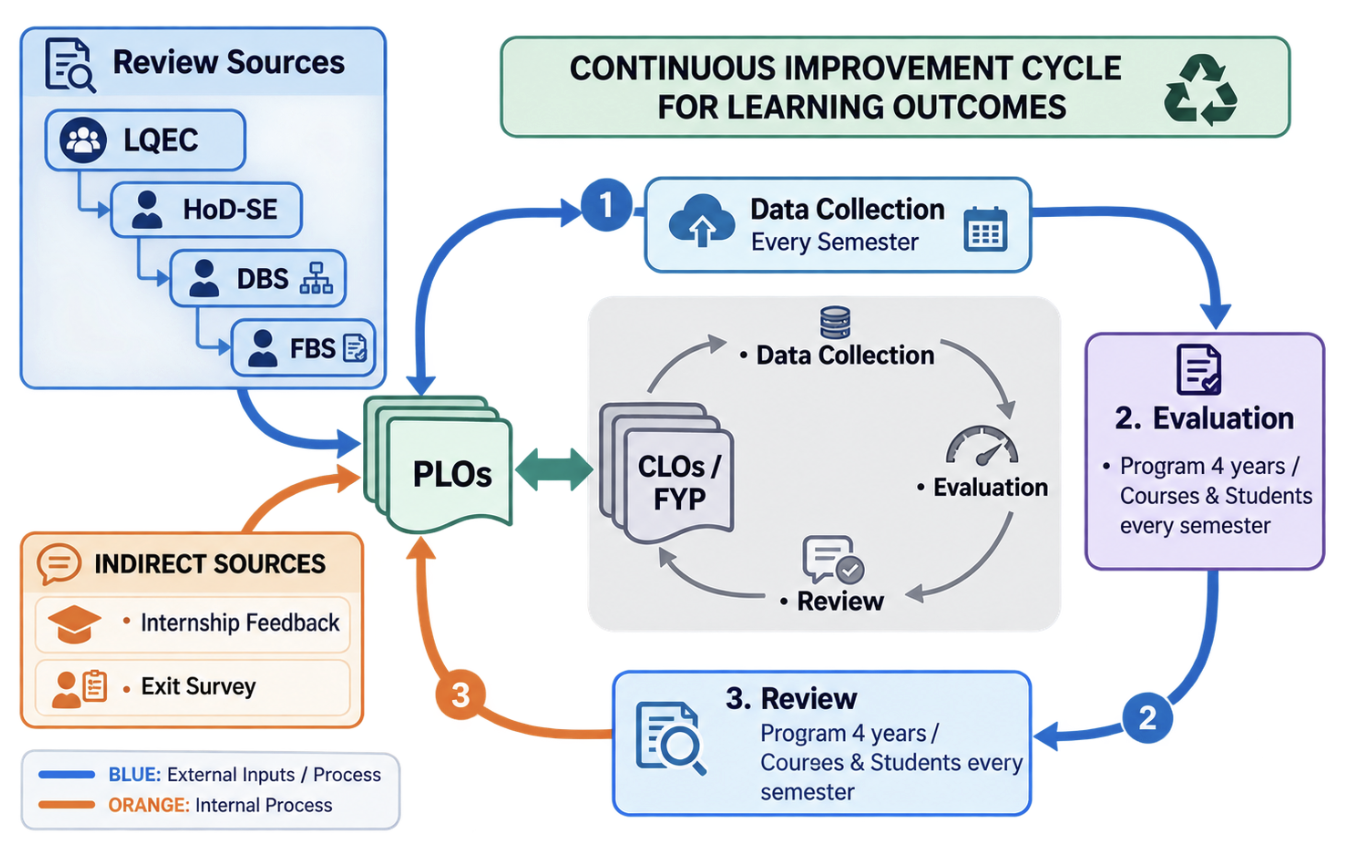
\includegraphics[width=0.80\textwidth]{images/front_matter/media/image-15.png}
\caption{PLO Assessment, Review, Stakeholder Involvement, and CQI}
\label{fig:plo-cqi-process}
\end{figure}

%-----------------------------------------------------------------------
\hypertarget{sec:cloplo}{%
\section{Mapping of Courses to PLOs}\label{sec:cloplo}}

To ensure comprehensive coverage of all 11 Program Learning Outcomes (PLOs), courses are systematically designed and mapped to relevant PLOs through their Course Learning Outcomes (CLOs). Rather than mapping every course to all PLOs, the curriculum adopts a structured, progressive approach in which selected courses contribute to the attainment of specific graduate attributes throughout the program.

The mapping of selected courses used for PLO assessment is presented in Table~\ref{table:courses-to-plo-mapping}. It demonstrates how individual CLOs contribute to relevant PLOs and how graduate attributes are developed across the curriculum. In addition to coursework, relevant PLOs are mapped to the Final Year Design Project (FYDP) evaluation rubrics used in Semesters 7 and 8. These rubrics assess students' attainment of the applicable graduate attributes at different stages of project development, providing evidence of their ability to apply engineering knowledge, solve complex problems, work collaboratively, and demonstrate professional competencies, as relevant to the mapped PLOs.

CLO achievement provides direct evidence of student learning and is systematically reviewed through the Continuous Quality Improvement (CQI) process. Assessment results help identify performance gaps, evaluate teaching and assessment strategies, and determine corrective actions where required. Similarly, FYDP rubric results contribute to evaluating PLO attainment through students' project planning, design, implementation, and final evaluation.

Course outlines are prepared by the concerned faculty in consultation with the Local Quality Enhancement Cell (LQEC) to ensure alignment with program objectives, relevant PLOs, and institutional quality assurance requirements. These outlines are reviewed and approved by the Head of Department (HoD). Subsequent revisions arising from course assessment, stakeholder feedback, or CQI recommendations are incorporated through the established review and approval process. A sample course outline is provided in Annexure~\ref{app:criteria-3_Course Outline with Knowledge Group Head's Signature}. Table~\ref{table:elective mapping} presents the mapping of CLOs of all specialization courses to PLOs, with equal weightage assigned to each contributing course outcome.

% Table 3.3: Course-to-PLO Mapping (wide table -- landscape + scriptsize)
\clearpage
\begin{landscape}
\begingroup\scriptsize\setlength{\tabcolsep}{2.5pt}
\begin{longtable}{>{\raggedright\arraybackslash}p{0.075\linewidth}
                  >{\raggedright\arraybackslash}p{0.165\linewidth}
                  >{\centering\arraybackslash}p{0.055\linewidth}
                  >{\centering\arraybackslash}p{0.055\linewidth}
                  >{\centering\arraybackslash}p{0.055\linewidth}
                  >{\centering\arraybackslash}p{0.055\linewidth}
                  >{\centering\arraybackslash}p{0.055\linewidth}
                  >{\centering\arraybackslash}p{0.055\linewidth}
                  >{\centering\arraybackslash}p{0.055\linewidth}
                  >{\centering\arraybackslash}p{0.055\linewidth}
                  >{\centering\arraybackslash}p{0.055\linewidth}
                  >{\centering\arraybackslash}p{0.055\linewidth}
                  >{\centering\arraybackslash}p{0.055\linewidth}
                  >{\centering\arraybackslash}p{0.065\linewidth}}
\caption{Mapping of Courses to PLOs and Appropriate BT Domain \& BT Level} \\
\toprule
\textbf{Code} & \textbf{Course Title} & \textbf{PLO 1} & \textbf{PLO 2} & \textbf{PLO 3} & \textbf{PLO 4} & \textbf{PLO 5} & \textbf{PLO 6} & \textbf{PLO 7} & \textbf{PLO 8} & \textbf{PLO 9} & \textbf{PLO 10} & \textbf{PLO 11} & \textbf{WKs} \\
& & \scriptsize Eng. Know. & \scriptsize Prob. Anal. & \scriptsize Design/ Dev. & \scriptsize Invest. & \scriptsize Tool Usage & \scriptsize Eng. \& World & \scriptsize Ethics & \scriptsize Teamwork & \scriptsize Commun. & \scriptsize Proj. Mgmt. & \scriptsize Lifelong Learn. & \\
\midrule
\endfirsthead
\multicolumn{14}{l}{\footnotesize\textit{Continued from previous page}} \\
\toprule
\textbf{Code} & \textbf{Course Title} & \textbf{PLO 1} & \textbf{PLO 2} & \textbf{PLO 3} & \textbf{PLO 4} & \textbf{PLO 5} & \textbf{PLO 6} & \textbf{PLO 7} & \textbf{PLO 8} & \textbf{PLO 9} & \textbf{PLO 10} & \textbf{PLO 11} & \textbf{WKs} \\
\midrule
\endhead
\midrule\multicolumn{14}{r}{\footnotesize\textit{Continued on next page}} \\
\endfoot
\bottomrule
\endlastfoot
\multicolumn{14}{l}{\textbf{Semester 1}} \\
CS-117   & Applications of ICT                       & C-2 & C-4 &     &     &     &     &     & A-3 &     &     &     & WK-2 \\
HU-131   & Fehm-ul-Quran I                           &     &     &     &     &     &     &     &     &     &     & C-2 & WK-7 \\
HU-101   & Islamic Studies                           &     &     &     &     &     & C-4 & A-3 &     &     &     & C-2 & WK-7 \\
CS-110   & Fundamentals of Computer Programming      & C-2 & C-3 &     &     & P-3 &     &     & A-2 &     &     &     & WK-2 \\
MATH-101 & Calculus and Analytical Geometry          & C-2, C-3 & C-4 &   &   &   &   &   &   &   &   &   & WK-2 \\
PH-102   & Applied Physics                           &     & C-3, C-3 & P-3 & & &  &  &  &  &  &  & WK-2 \\
HU-127   & Ideology and Constitution of Pakistan     &     &     &     &     &     & A-2 &     &     &     &     & C-4 & WK-7 \\
\multicolumn{14}{l}{\textbf{Semester 2}} \\
CS-212   & Object Oriented Programming               & C-2 & C-5 & C-6 &     & P-3 &     & A-3 &     &     &     &     & WK-3 \\
HU-132   & Fehm-e-Quran-II                           &     &     &     &     &     &     &     &     &     &     & C-2 & WK-7 \\
MATH-121 & Linear Algebra and ODEs                   & C-2 & C-3 & C-3 &     &     &     &     &     &     &     &     & WK-2 \\
MATH-161 & Discrete Mathematics                      & C-2 & C-4 & C-3 &     &     &     &     &     &     &     &     & WK-2 \\
HU-114   & Functional English                        &     &     &     &     &     &     &     &     & A-2 &     & C-2, C-3 & WK-7 \\
EE-122   & Computer Architecture and Logic Design    & C-3 & C-4 & C-5 & P-4 &  P-4   &     & A-3 & A-3 &     &     &     & WK-3 \\
\multicolumn{14}{l}{\textbf{Semester 3}} \\
CS-220   & Database Systems                          & C-2 &     & C-3 & C-5 & P-3 &     &     &     &     &     &     & WK-3 \\
SE-200   & Software Engineering                      & C-2 & C-4 & C-3 & C-5 &     &     &     & A-3 &     &     &     & WK-4 \\
CS-250   & Data Structures \& Algorithms             & C-2 &     & C-3   &  & P-4 &     & A-3 & A-2 &     &     &     & WK-3 \\
MATH-232 & Complex Variables and Transform           & C-3 & C-4 & C-5 &     &     &     &     &     &     &     &     & WK-2 \\
EE-353   & Computer Networks                         & C-3 &     & C-6 & C-4 & P-4 &     &     &     &     &     &     & WK-3 \\
\multicolumn{14}{l}{\textbf{Semester 4}} \\
CS-330   & Operating Systems                         & C-2 & C-4 &     & C-5 & P-3 &     &     &     &     &     &     & WK-3 \\
CS-251   & Design \& Analysis of Algorithm           &     & C-4 & C-6 & C-5 &     &     &     &     &     &     &     & WK-4 \\
HU-107   & Pakistan Studies                          &     &     &     &     &     &  & A-2 &     &     &     & C-2 & WK-7 \\
SE-211   & Software Design and Architecture          & C-2 & C-4 & C-3 & C-5 &     &     &     &     &     &     &     & WK-4 \\
MATH-361 & Probability and Statistics                & C-2 & C-4 & C-3 &     &     &     &     &     &     &     &     & WK-2 \\
ENGL-104 & Expository Writing                        &     &     &     &     &     & C-4 & C-3 &     & A-4    &     &  & WK-7 \\
\multicolumn{14}{l}{\textbf{Semester 5}} \\
MGT-121  & Introduction to Management                &     & C-4 &     &     &     &     &     &     & A-2 & A-3 & C-2 & WK-7 \\
CS-344   & Web Engineering*                          & C-2 & C-3 &     & C-4 & P-4 &     &     & A-2 &     &     &     & WK-5 \\
SE-315   & Cloud Computing                           & C-2 & C-3 &     & C-4 & P-4 &     &     &     &     &     &     & WK-4 \\
CS-336   & Embedded Systems                          & C-2, C-3 &  &  & P-4 & P-4 &  &  &  &  &  &  & WK-4 \\
HU-222   & Professional Ethics                       &     &     &     &     &     & C-4 & C-3 &     &     &     & A-3 & WK-7 \\
SE-314   & Software Construction                     & C-2 & C-3 & C-6 &     & P-3 &     &     &     &     &     &     & WK-4 \\
\multicolumn{14}{l}{\textbf{Semester 6}} \\
MGT-271  & Entrepreneurship                          &     &  C-4   &  C-3   &     &     & C-2  &  &  & A-3 & C-6 &  & WK-7 \\
SE-320   & Formal Methods                            & C-2 &     & C-6 & C-4 & P-3 &     &     &     &     &     &     & WK-3 \\
CS-471   & Machine Learning*                         & C-3 & C-4 & C-6 &     & P-4 &     &     &     &     &     &     & WK-5 \\
CS-261   & Human Computer Interaction                & C-2 & C-4 & C-6 &     & P-3 &     &     &     &     &     &     & WK-4 \\
SE-430   & Software Project Management               & C-2 &     &     & C-4 & C-5 &     &     & A-5 &     & A-3 &     & WK-4 \\
SE-321   & Software Quality Engg.                    & C-3 & C-4 & C-6 &     &     & A-3 &     &     &     &     &     & WK-4 \\
\multicolumn{14}{l}{\textbf{Semester 7}} \\
SE-498   & Final Year Design Project -- 1            & $\checkmark$ & $\checkmark$ & $\checkmark$ & $\checkmark$ & $\checkmark$ & $\checkmark$ &  & $\checkmark$ & $\checkmark$ & $\checkmark$ & & WK-6/7/8 \\
CS-484   & Information Security                      & C-2 &     & C-6 & C-4 &     &     &     &     &     &     &     & WK-4 \\
CS-365   & Virtual \& Augmented Reality*             & C-2 & C-4 & C-6 &     & P-4 &     &     &     &     &     &     & WK-6 \\
MATH-352 & Numerical Methods                         & C-3 & C-4 &  &     & P-4 &     &     &     &     &     &     & WK-2 \\
CS-335   & Internet of Things*                       & C-2 & C-4 & C-6 & C-5 &     &     &     &     &     &     &     & WK-4 \\
CS-381   & Network Security*                         & C-3 &     & C-6 & C-5 & P-3 &     &     &     &     &     &     & WK-5 \\
\multicolumn{14}{l}{\textbf{Semester 8}} \\
SE-499   & Final Year Design Project -- 2            & $\checkmark$ & $\checkmark$ & $\checkmark$ & $\checkmark$ & $\checkmark$ & $\checkmark$ & $\checkmark$ & $\checkmark$ & $\checkmark$ & $\checkmark$ & $\checkmark$ & WK-6/7/8 \\
ECO-130  & Engineering Economics*                    & C-2 & C-4 &     &     &     &     &     &     &     & C-5 &     & WK-7 \\
CS-416   & Large Language Models*                    & C-2 & C-4 & C-3 & C-5 & P-4 &     &     & C-6 &     &     &     & WK-6 \\
CCE-401  & Civic \& Community Engagement             &     &     &     &     &     & A-3, A-4 &     &     &     &    &     & WK-7 \\
OHS-101  & Occupation Health \& Safety               &     &     &     &     &     & C-3, C-2 &  &  &  &  &  & WK-3 \\
CS-415   & Mobile Application Development*           & C-2 &     & C-6 & C-4 & P-4 &     &     &     &     &     &     & WK-6 \\
\midrule
         & \textbf{Total}                            & \textbf{36} & \textbf{30} & \textbf{27} & \textbf{19} & \textbf{22} & \textbf{12} & \textbf{8} & \textbf{10} & \textbf{6} & \textbf{6} & \textbf{10} & \\
\label{table:courses-to-plo-mapping}
\end{longtable}

\vspace{12pt}
\textbf{*Elective Depth Courses}

\begin{longtable}{>{\raggedright\arraybackslash}p{0.075\linewidth}
                  >{\raggedright\arraybackslash}p{0.165\linewidth}
                  >{\centering\arraybackslash}p{0.055\linewidth}
                  >{\centering\arraybackslash}p{0.055\linewidth}
                  >{\centering\arraybackslash}p{0.055\linewidth}
                  >{\centering\arraybackslash}p{0.055\linewidth}
                  >{\centering\arraybackslash}p{0.055\linewidth}
                  >{\centering\arraybackslash}p{0.055\linewidth}
                  >{\centering\arraybackslash}p{0.055\linewidth}
                  >{\centering\arraybackslash}p{0.055\linewidth}
                  >{\centering\arraybackslash}p{0.055\linewidth}
                  >{\centering\arraybackslash}p{0.055\linewidth}
                  >{\centering\arraybackslash}p{0.055\linewidth}
                  >{\centering\arraybackslash}p{0.065\linewidth}}
\caption{Elective Depth Courses -- PLO Mapping} 
\label{table:elective mapping}
\\
\toprule
\textbf{Code} & \textbf{Course Title} & \textbf{PLO 1} & \textbf{PLO 2} & \textbf{PLO 3} & \textbf{PLO 4} & \textbf{PLO 5} & \textbf{PLO 6} & \textbf{PLO 7} & \textbf{PLO 8} & \textbf{PLO 9} & \textbf{PLO 10} & \textbf{PLO 11} & \textbf{WKs} \\
\midrule
\endfirsthead
\multicolumn{14}{l}{\footnotesize\textit{Continued from previous page}} \\
\toprule
\textbf{Code} & \textbf{Course Title} & \textbf{PLO 1} & \textbf{PLO 2} & \textbf{PLO 3} & \textbf{PLO 4} & \textbf{PLO 5} & \textbf{PLO 6} & \textbf{PLO 7} & \textbf{PLO 8} & \textbf{PLO 9} & \textbf{PLO 10} & \textbf{PLO 11} & \textbf{WKs} \\
\midrule
\endhead
\midrule\multicolumn{14}{r}{\footnotesize\textit{Continued on next page}} \\
\endfoot
\bottomrule
\endlastfoot
EC-303  & Mobile Application Development for SMEs & C-2 &     & C-6 & C-4 & P-4 &  &  &  &  &  &  & WK-6 \\
CS-335  & Internet of Things     & C-2 & C-4 & C-6 & C-5 &     &  &  &  &  &  &  & WK-4 \\
CS-344  & Web Engineering        & C-2 & C-3 &     & C-4 & P-4 &  &  & A-2 &  &  &  & WK-5 \\
CS-365  & Virtual and Augmented Reality & C-2 & C-4 & C-6 &  & P-4 &  &  &  &  &  &  & WK-6 \\
CS-368  & Reinforcement Learning & C-3 & C-4 & C-6 &     & P-3 &  &  &  &  &  &  & WK-6 \\
CS-381  & Network Security       & C-3 &     & C-6 & C-5 & P-3 &  &  &  &  &  &  & WK-5 \\
CS-405  & Deep Learning          & C-3 & C-4 & C-6 &     & P-4 &  &  &  &  &  &  & WK-6 \\
CS-416  & Large Language Models  & C-2 & C-4 & C-3 & C-5 & P-4 &  &  & C-6 &  &  &  & WK-6 \\
CS-471  & Machine Learning       & C-3 & C-4 & C-6 &     & P-4 &  &  &  &  &  &  & WK-5 \\
CS-481  & Computer Forensics     & C-2 &     &     & C-3 & P-3 &  &  &  &  &  &  & WK-6 \\
\end{longtable}
\endgroup
\end{landscape}

%-----------------------------------------------------------------------
\hypertarget{sec:datagathering}{%
\section{Data Gathering and Results Analysis for PLO Assessment}\label{sec:datagathering}}

The PLOs are assessed using both direct and indirect assessment methods, as presented in Table~\ref{table: KPI for PLO attainment}. Direct assessment at the individual student level is used to evaluate and monitor the attainment of PLOs by each student. At the cohort (batch) level, direct assessment is used to identify gaps, deficiencies, or areas of concern within the academic program. Indirect assessment, on the other hand, is used to evaluate the overall effectiveness of the program and to identify opportunities for Continuous Quality Improvement (CQI).

At the time of graduation, all students are expected to attain all PLOs in accordance with the defined Key Performance Indicators (KPIs) for both direct and indirect assessment methods. The course-level assessment results are systematically reviewed to identify areas requiring improvement. Based on the findings, the LQEC proposes corrective and improvement measures, which are subsequently presented to the DBS for discussion, deliberation, and approval.

A detailed description of the direct and indirect assessment methods, along with their respective processes and mechanisms, is provided below..

\begin{table}[H]
\centering
\setlength{\tabcolsep}{3pt}
\caption{KPI for PLO Attainment}
\footnotesize
\begin{tabular}{>{\raggedright\arraybackslash}p{0.12\textwidth}
                >{\raggedright\arraybackslash}p{0.17\textwidth}
                >{\centering\arraybackslash}p{0.12\textwidth}
                >{\raggedright\arraybackslash}p{0.40\textwidth}
                >{\raggedright\arraybackslash}p{0.11\textwidth}}
\toprule
\textbf{PLOs} & \textbf{Measurement Tools} & \textbf{Method} & \textbf{KPIs} & \textbf{When Measured} \\
\midrule
1 to 11 & Exams/FYDP & Direct &
Cohort -- at least 60\% of cohort should attain minimum 50\% for a PLO. & At graduation\\
&&&Individual -- each student should attain minimum 50\% in all PLOs. &  \\
\addlinespace
 & Internship Feedback & Indirect &
Minimum 60\% of students attain score 3 and above on the scale of 1--5 for mapped PLOs & Annually \\
\addlinespace
 & Exit Survey & Indirect &
Minimum 60\% of students attain score 3 and above on the scale of 1--5 for each PLO & At graduation \\
\bottomrule
\end{tabular}
\label{table: KPI for PLO attainment}
\end{table}

\hypertarget{sec:directassess}{%
\section{Direct PLO Assessment}\label{sec:directassess}}

The direct method of assessment is accomplished directly through coursework (examinations and rubrics) and FYDP rubrics.

\subsection{Assessment via Coursework (CLOs)}

The course results are all managed on Qalam, an in-house campus management system that prepares OBE results (i.e., generating semester-wise or batch-wise OBE attainment reports). All CLO \& PLO attainments are computed by the Qalam. The OBE configuration process on Qalam is discussed in detail in Annexure~\ref{OBE Assessment Configuration on Qalam}. The sample CLO report is provided in Annexure~\ref{Sample CLO Attainment Report} and the sample PLO report is given in Annexure~\ref{Sample PLO Attainment Report}. At the end of each academic semester, the result of attainment of CLOs and PLOs against each course is used by LQEC for monitoring individuals' results and for CQI process for PLOs on cohort level. OBE reports of all courses are kept by LQEC in soft forms.

The consolidated PLO attainment report for the 2022 batch after Fall 2025 (7\textsuperscript{th} semester) is provided in Annexure~\ref{Consolidated PLO Attainment Report}. It presents individual student scores for all 12 PLOs applicable to this batch. For each student, the attainment percentage for a PLO is calculated as the proportion of relevant assessment opportunities in which the student achieved the required benchmark. PLO attainment below 50\% is highlighted in red, enabling individual- and cohort-level analysis of deficiencies.

Direct PLO attainment is calculated from coursework and complemented by evidence from the FYDP, internship feedback, and graduate exit surveys. A student must achieve at least 50\% attainment in each PLO to meet the individual-level KPI. The CLO attainment KPIs are as follows:

\begin{enumerate}[label=\alph*.]
\item \textbf{Individual level: Each student passing a course is expected to achieve at least 50\% marks in each CLO.}
\item \textbf{Cohort level: At least 60\% of students passing a course must achieve at least 50\% marks in each CLO.}
\end{enumerate}

\subsection{Final Year Design Project (FYDP)\label{sec:FYDP}}

The PLOs attainment for FYDP is determined directly with the help of rubrics at various assessment stages during the course of the project. SEECS has a complete policy on methodology for conduct of FYDP, its assessments and evaluation. The details covering all aspects of FYDP are provided in Section~\ref{sec:4.11fydp}. At the award of the project students are provided with a handbook containing a detailed formatting guide and assessment rubrics for various assessment stages of the project over the last two semesters. Results for 7\textsuperscript{th} and 8\textsuperscript{th} semester are marked on the SEECS Thesis Management System (TMS). The assessment marks are directly mapped on PLOs. These marks are then manually exported to the Qalam to combine the PLO score assessed from courses and PLO score assessed from FYDP. Semester progress is marked several times by advisors and multiple evaluators during the whole semester. In addition to semester progress, various forms and rubrics are used for the assessment of proposal defense, mid semester defense, final defense, proposal document, SRS report, SDS report, final report, and defense presentations. Figure~\ref{figure:fydp} shows the roadmap of the FYDP milestones and deliverables over the course of 7\textsuperscript{th} and 8\textsuperscript{th} semesters.

\begin{figure}[H]
\centering
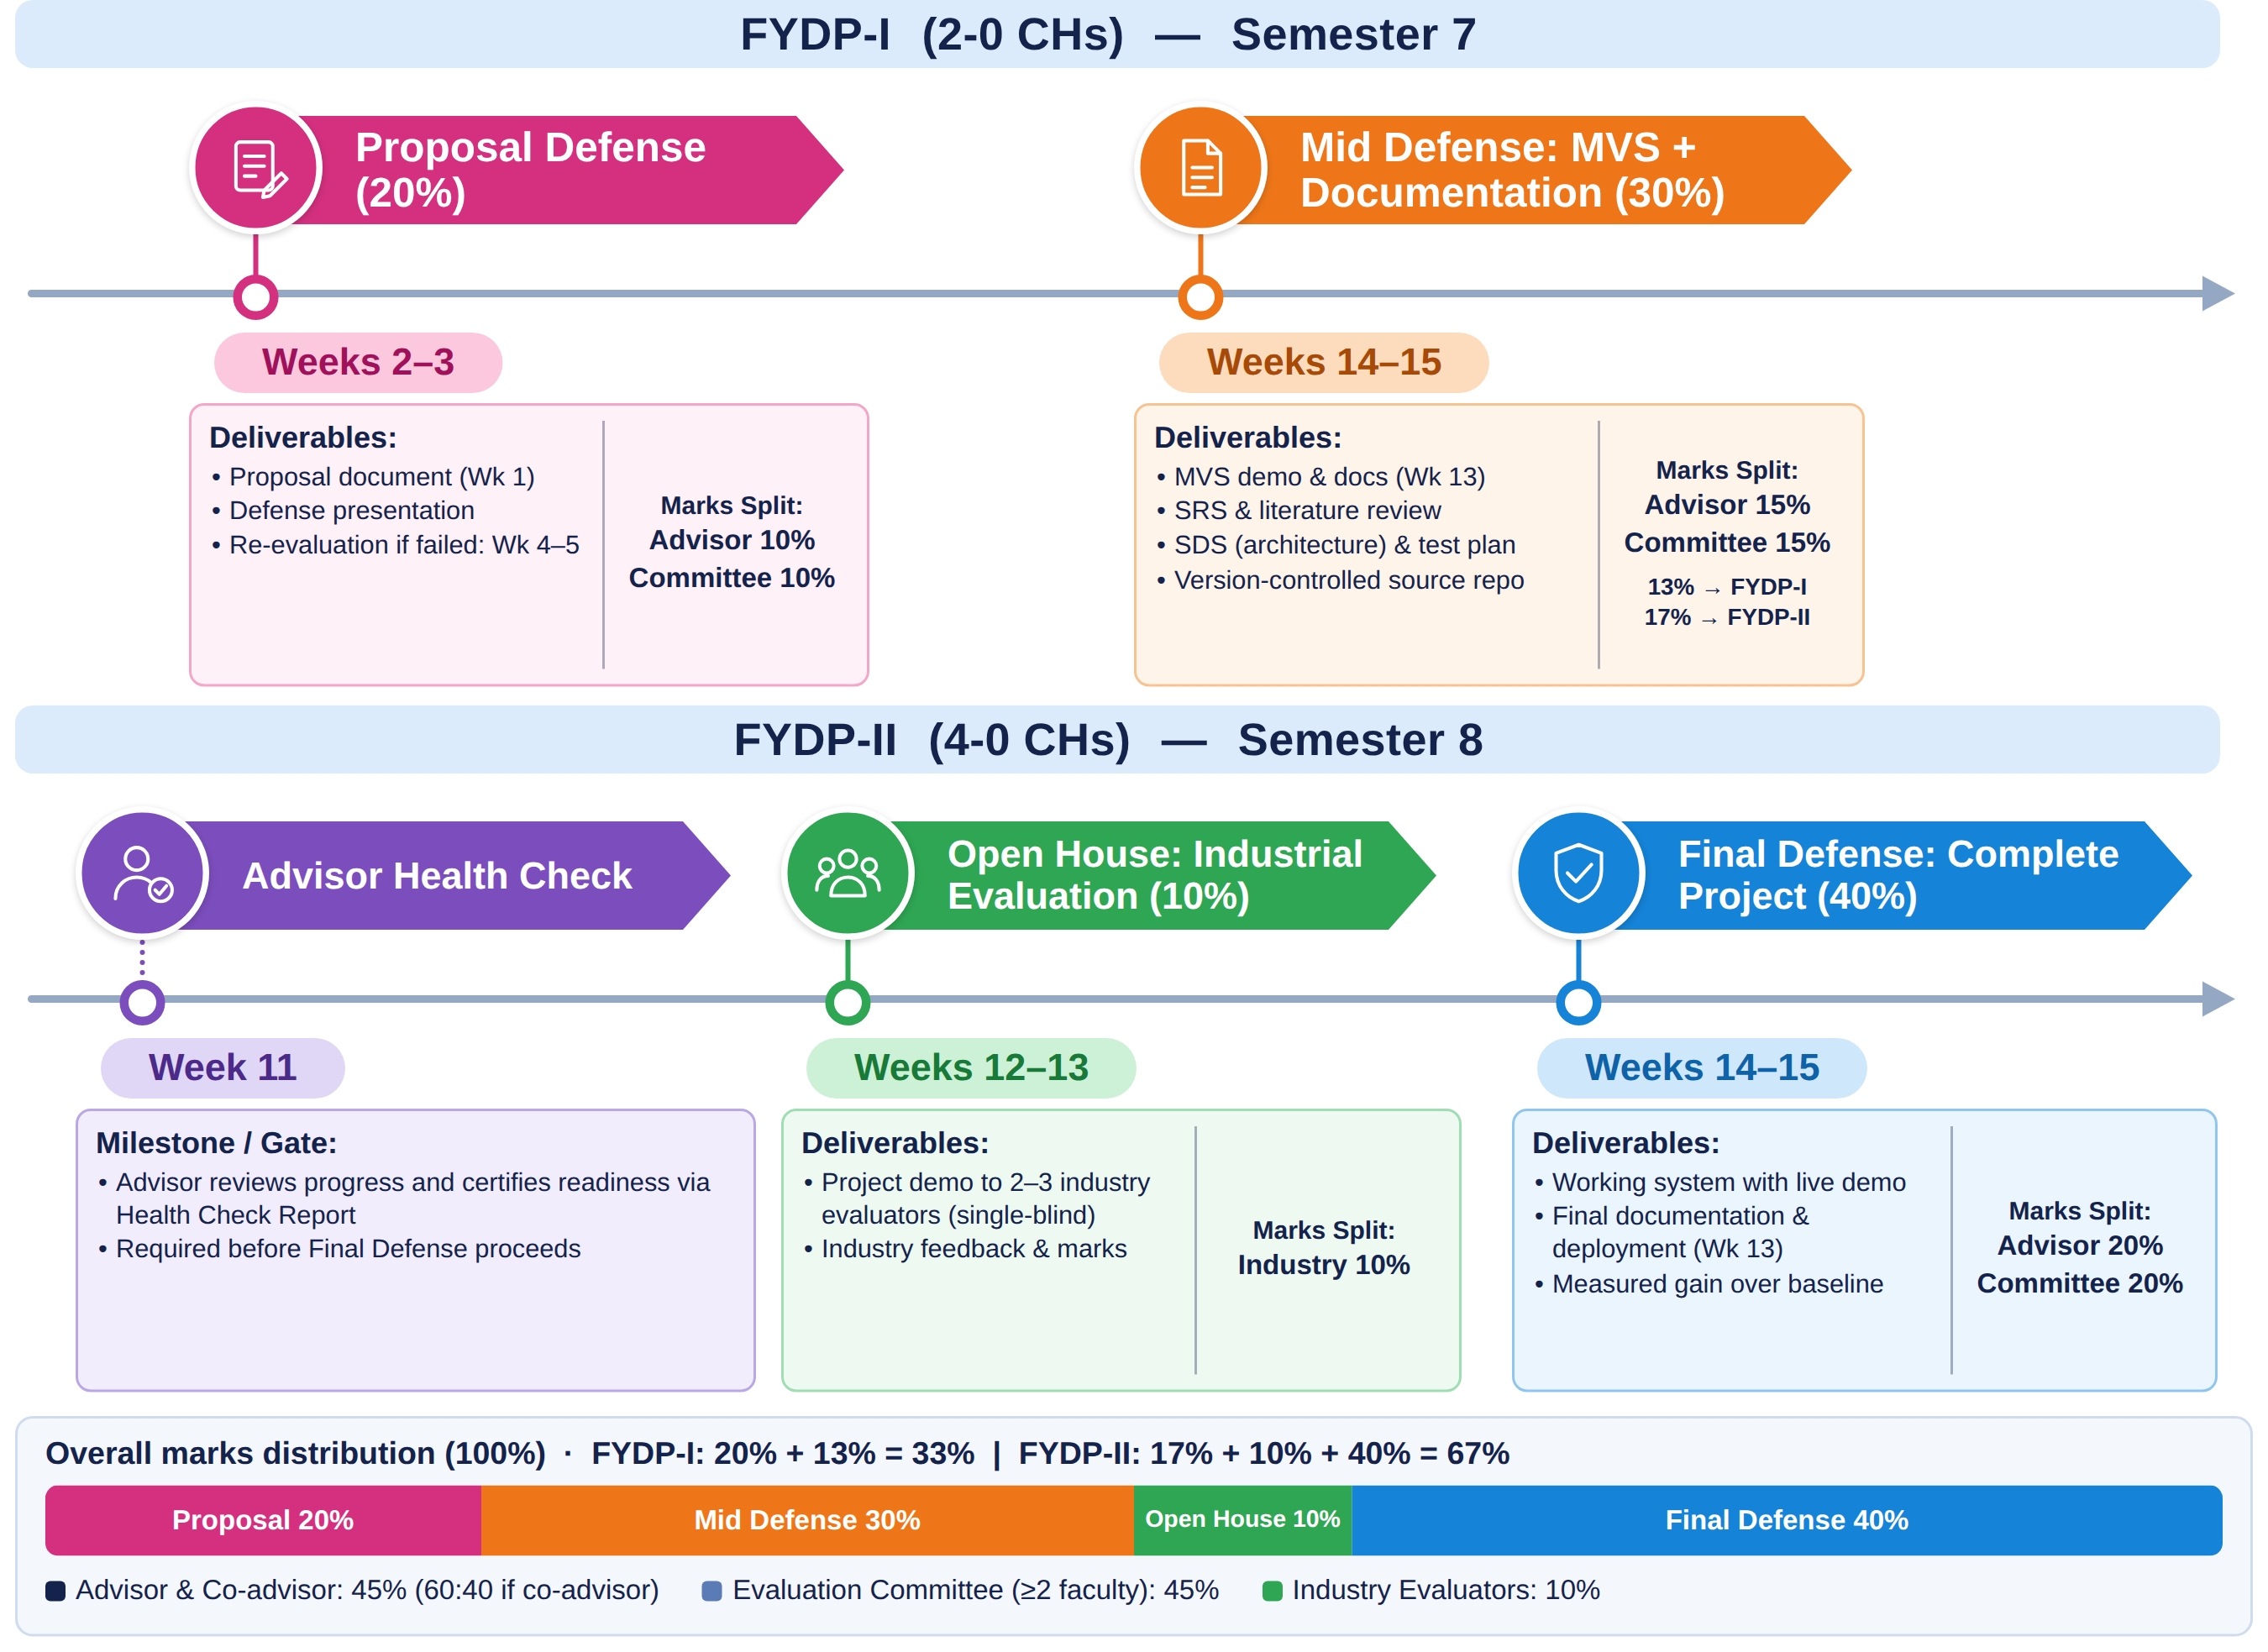
\includegraphics[width=1.0\textwidth]{images/criterion_2/media/FYDP-timeline.png}
\caption{Roadmap of Final Year Design Project (FYDP) Across 7\textsuperscript{th} \& 8\textsuperscript{th} Semesters.}
\label{figure:fydp}
\end{figure}
%-----------------------------------------------------------------------
\hypertarget{sec:fall2025results}{%
\subsection{CLO \& PLO Attainment Results for Fall 2025 Semester}\label{sec:fall2025results}}

\subsubsection{PLO Attainment at Cohort Level}

Results for Fall 2025 semester were prepared by the faculty using the OBE reports downloaded from the Qalam as mentioned in the previous sections. Data for cohort is extracted from the OBE reports and used for measurement of CLOs and PLOs attainment. The following section describe intake 2K23 batch results for attainment of CLOs and PLOs for Fall 2025 semester. The rest of the results of batch 2K22, 2K24, and 2K25 are provided in Annexure~\ref{annex:clo-plo-attainment-results}.

\paragraph{Fall 2025 Semester Results of Intake 2K23 Batch:} Figure~\ref{figure:2K23 Batch Result for All Courses} shows a screenshot of spreadsheet for all the courses taken by 2K23 batch in Fall 2025 semester. The figure contains CLO-PLO mapping and percentage of CLO attainment that is directly imported from the individual CLO and PLO attainment reports of each course from Qalam. Figure~\ref{figure:2K23 Batch cohort CLO attainment} shows same information as bar chart showing percentage attainment of corresponding CLOs against each course. Figure~\ref{figure:2K23 Batch Result for All Courses} also shows calculation of PLOs attainment as ``Ys'' as well as in percentage. The same information is given for PLO percentages and overall batch PLO attainment percentage in Figure~\ref{figure:2K23 Batch course-wise PLO attainment} and Figure~\ref{figure:2023 Batch cohort PLO attainment}, respectively. It can be seen that the cohort has successfully attained the concerned CLOs for each course. Similarly, the cohort PLOs have been attained as per set KPIs.


\begin{figure}[h]
\centering
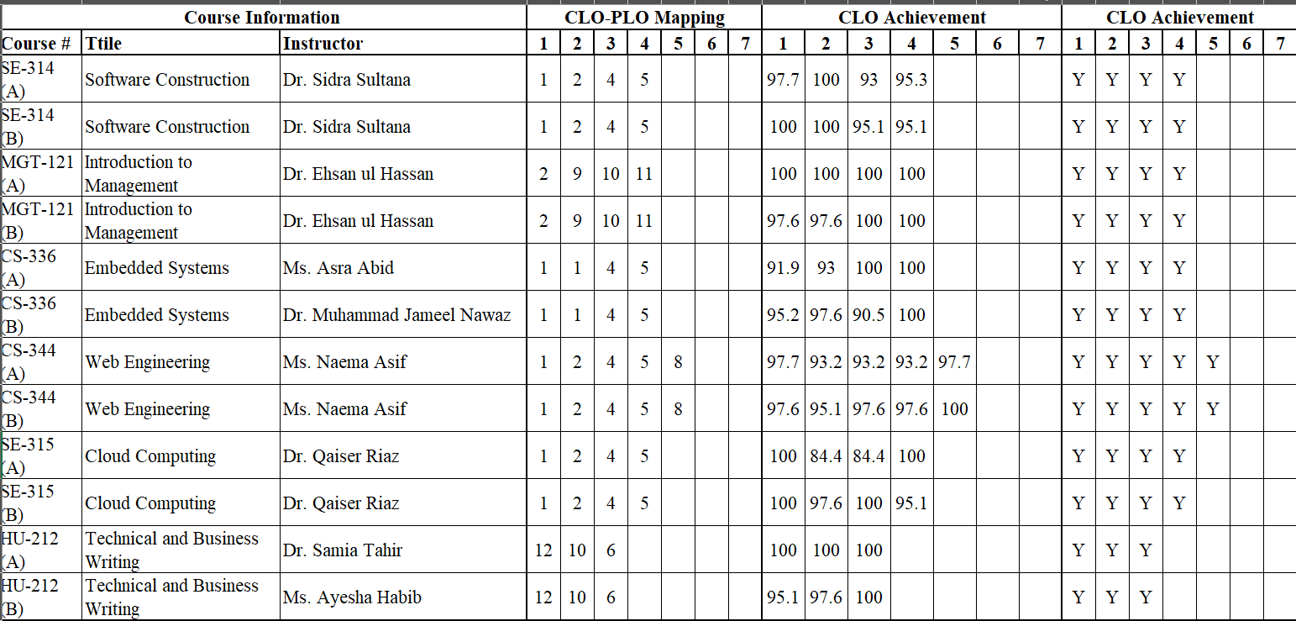
\includegraphics[width=0.98\linewidth]{images/criterion_2/media/image15.png}
\par\medskip
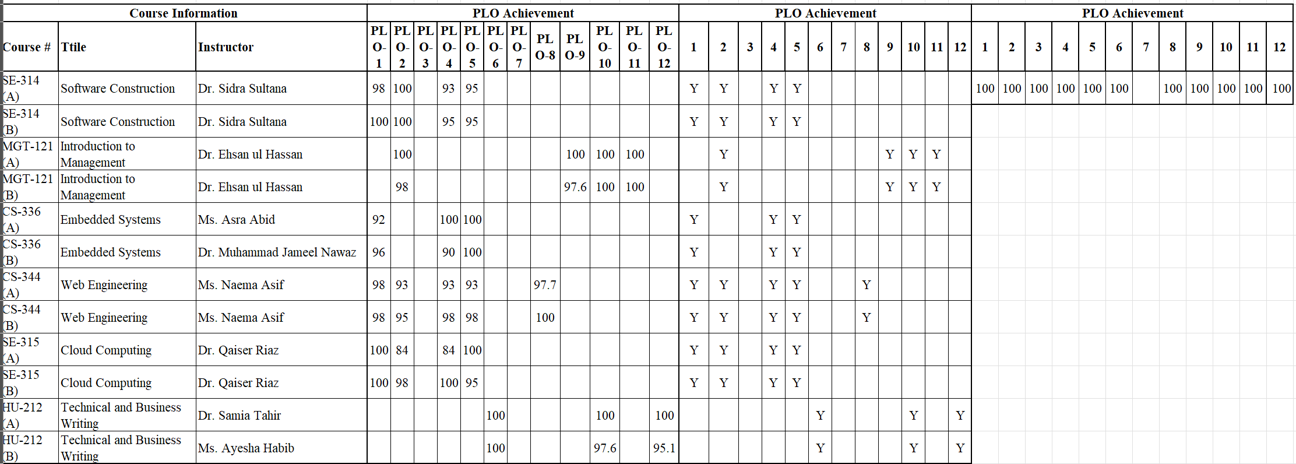
\includegraphics[width=0.98\linewidth]{images/criterion_2/media/image16.png}
\caption{2K23 Batch Result for All Courses in Fall 2025 Semester}
\label{figure:2K23 Batch Result for All Courses}
\end{figure}


\begin{figure}[H]
\centering
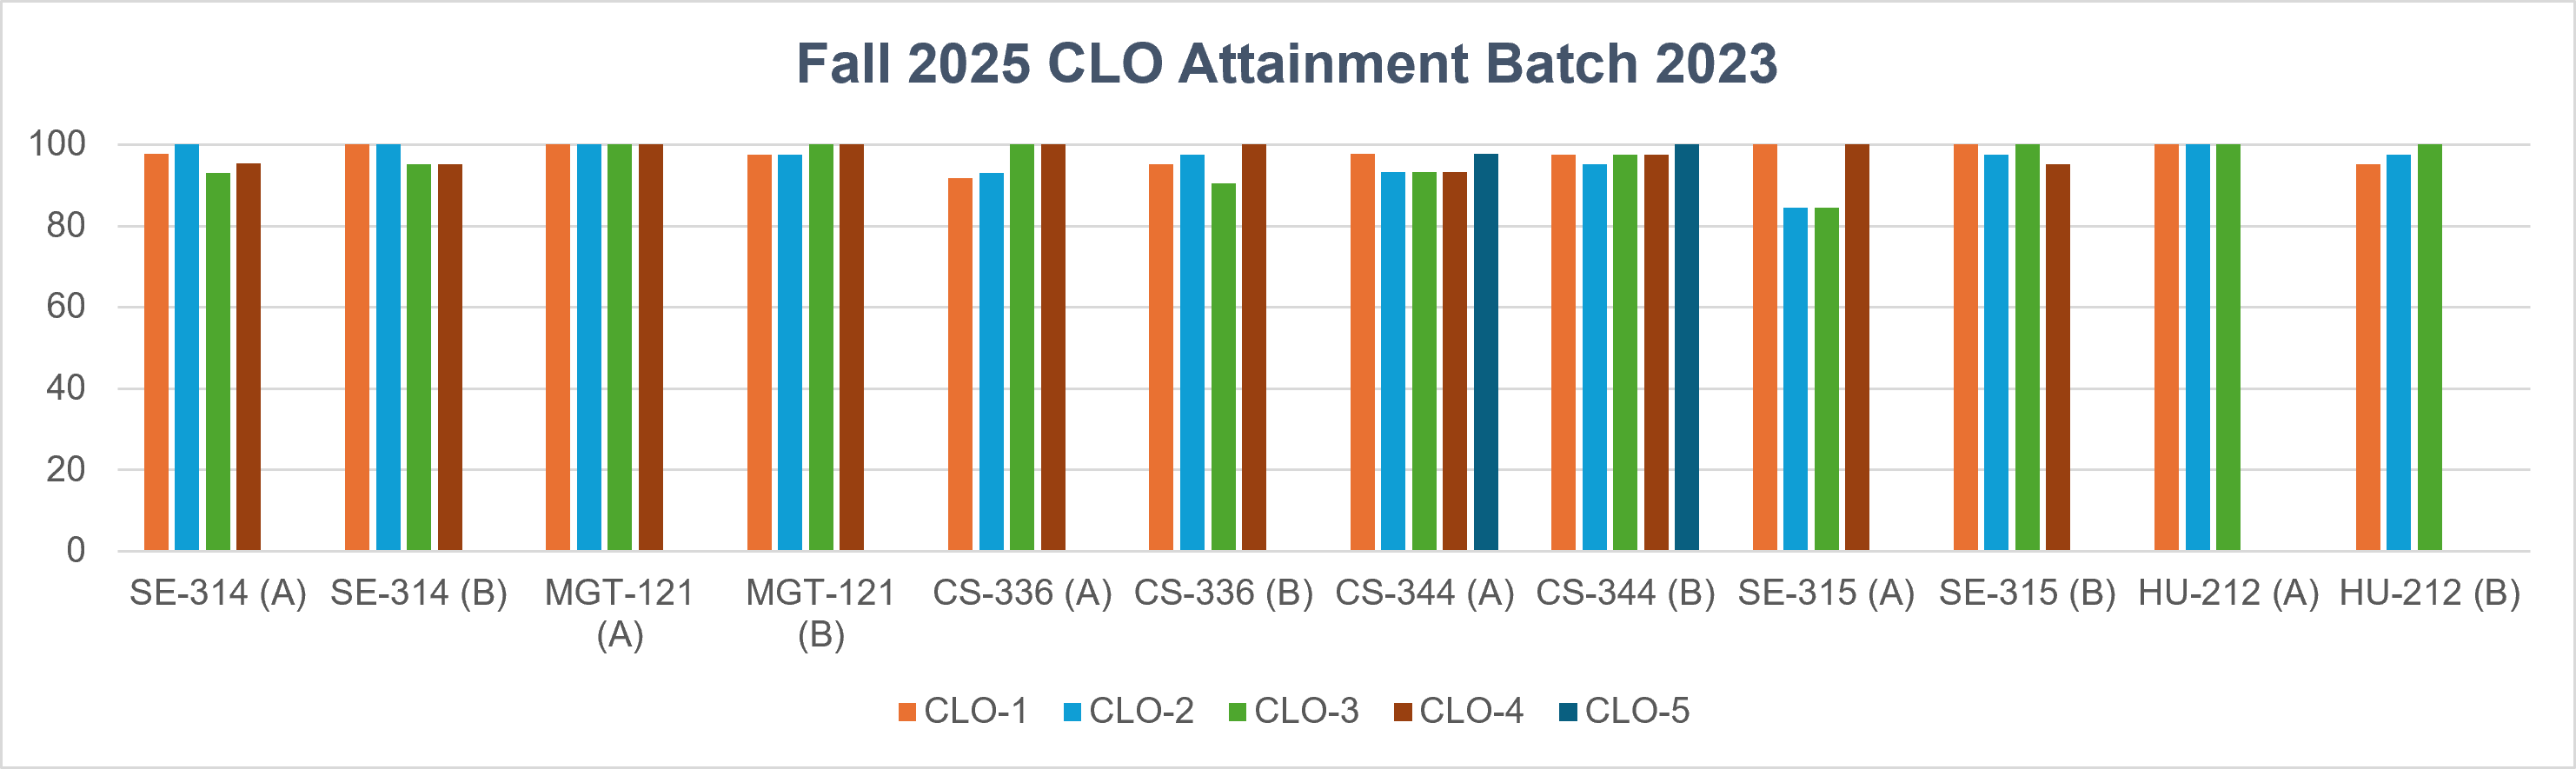
\includegraphics[width=0.97\textwidth]{images/criterion_2/media/image17.png}
\caption{2K23 Batch cohort CLO attainment for all courses in Fall 2025.}
\label{figure:2K23 Batch cohort CLO attainment}
\end{figure}

\begin{figure}[H]
\centering
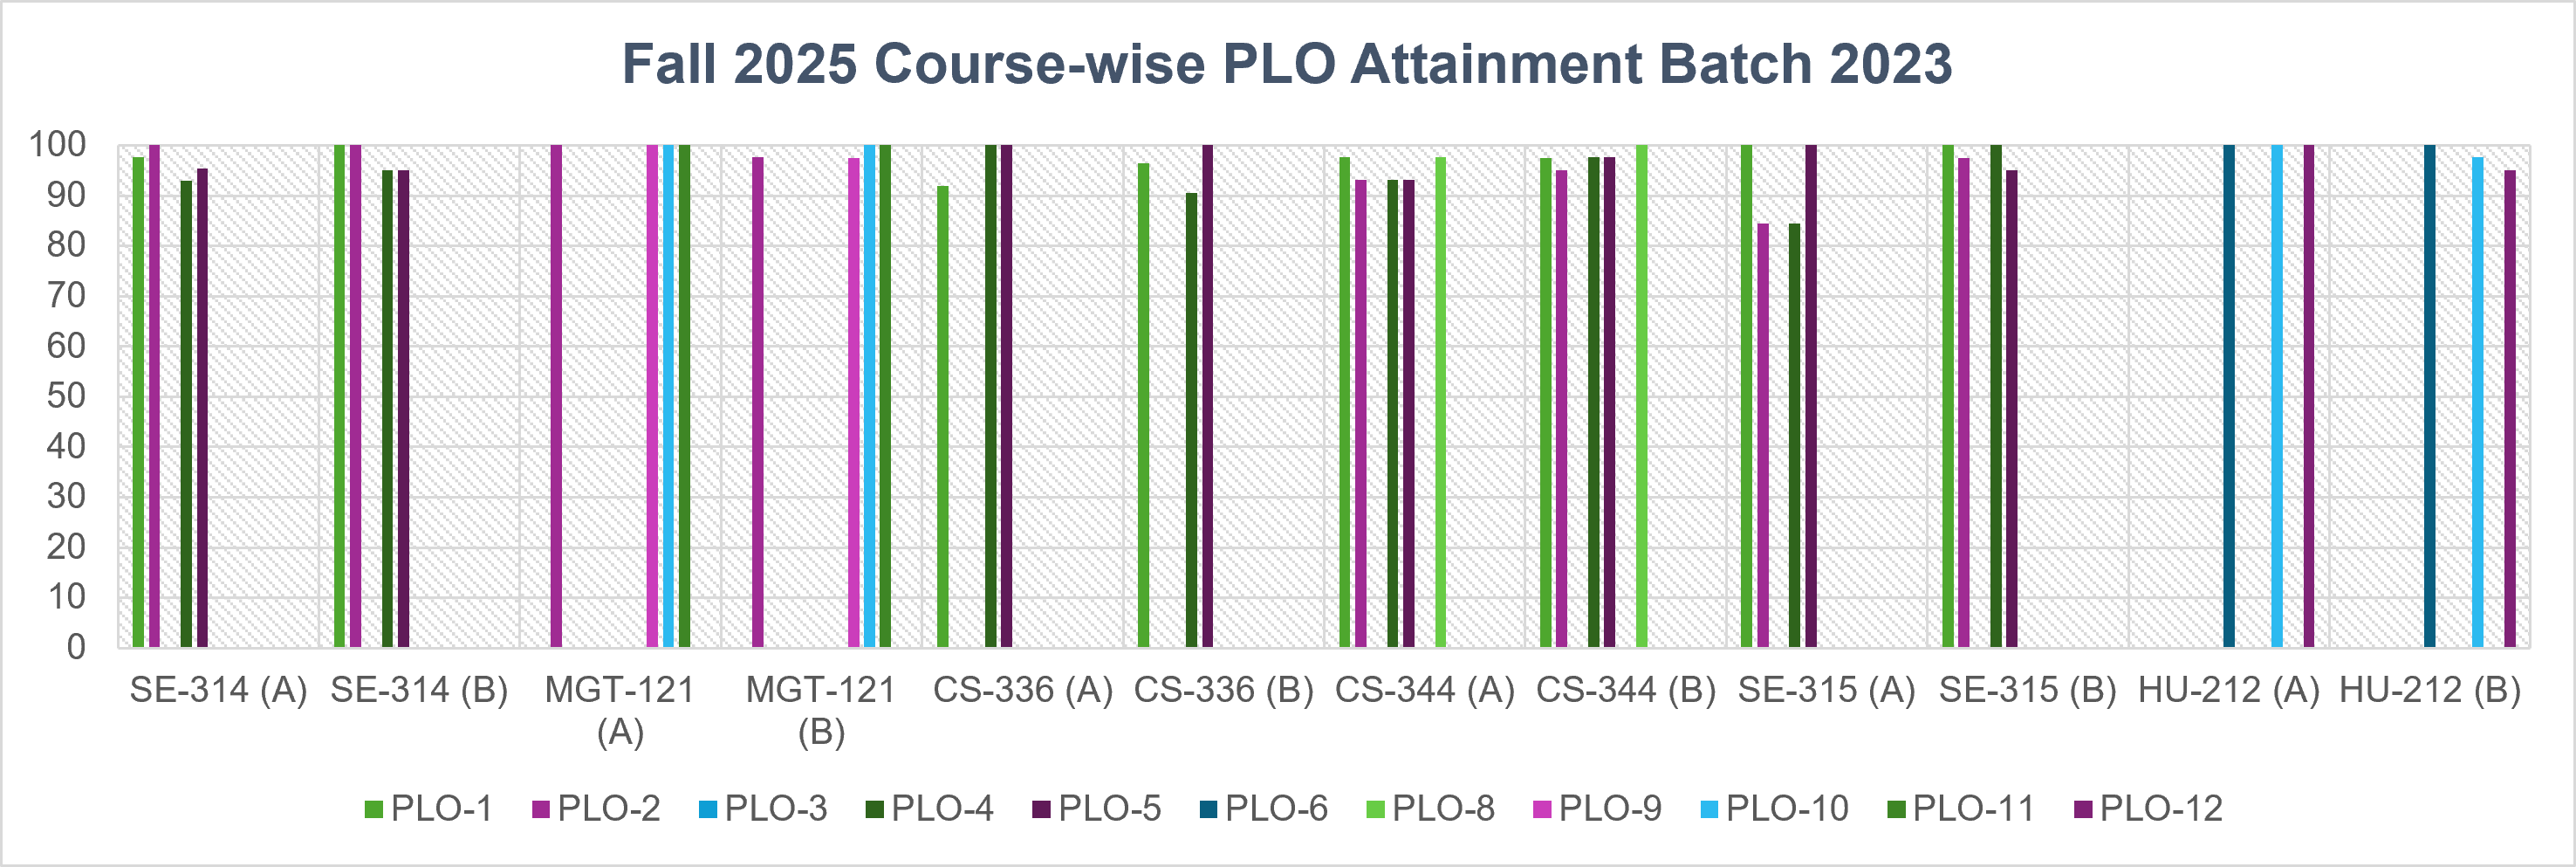
\includegraphics[width=0.98\textwidth]{images/criterion_2/media/image18.png}
\caption{2K23 Batch course-wise PLO attainment for Fall 2025.}
\label{figure:2K23 Batch course-wise PLO attainment}
\end{figure}

\begin{figure}[H]
\centering
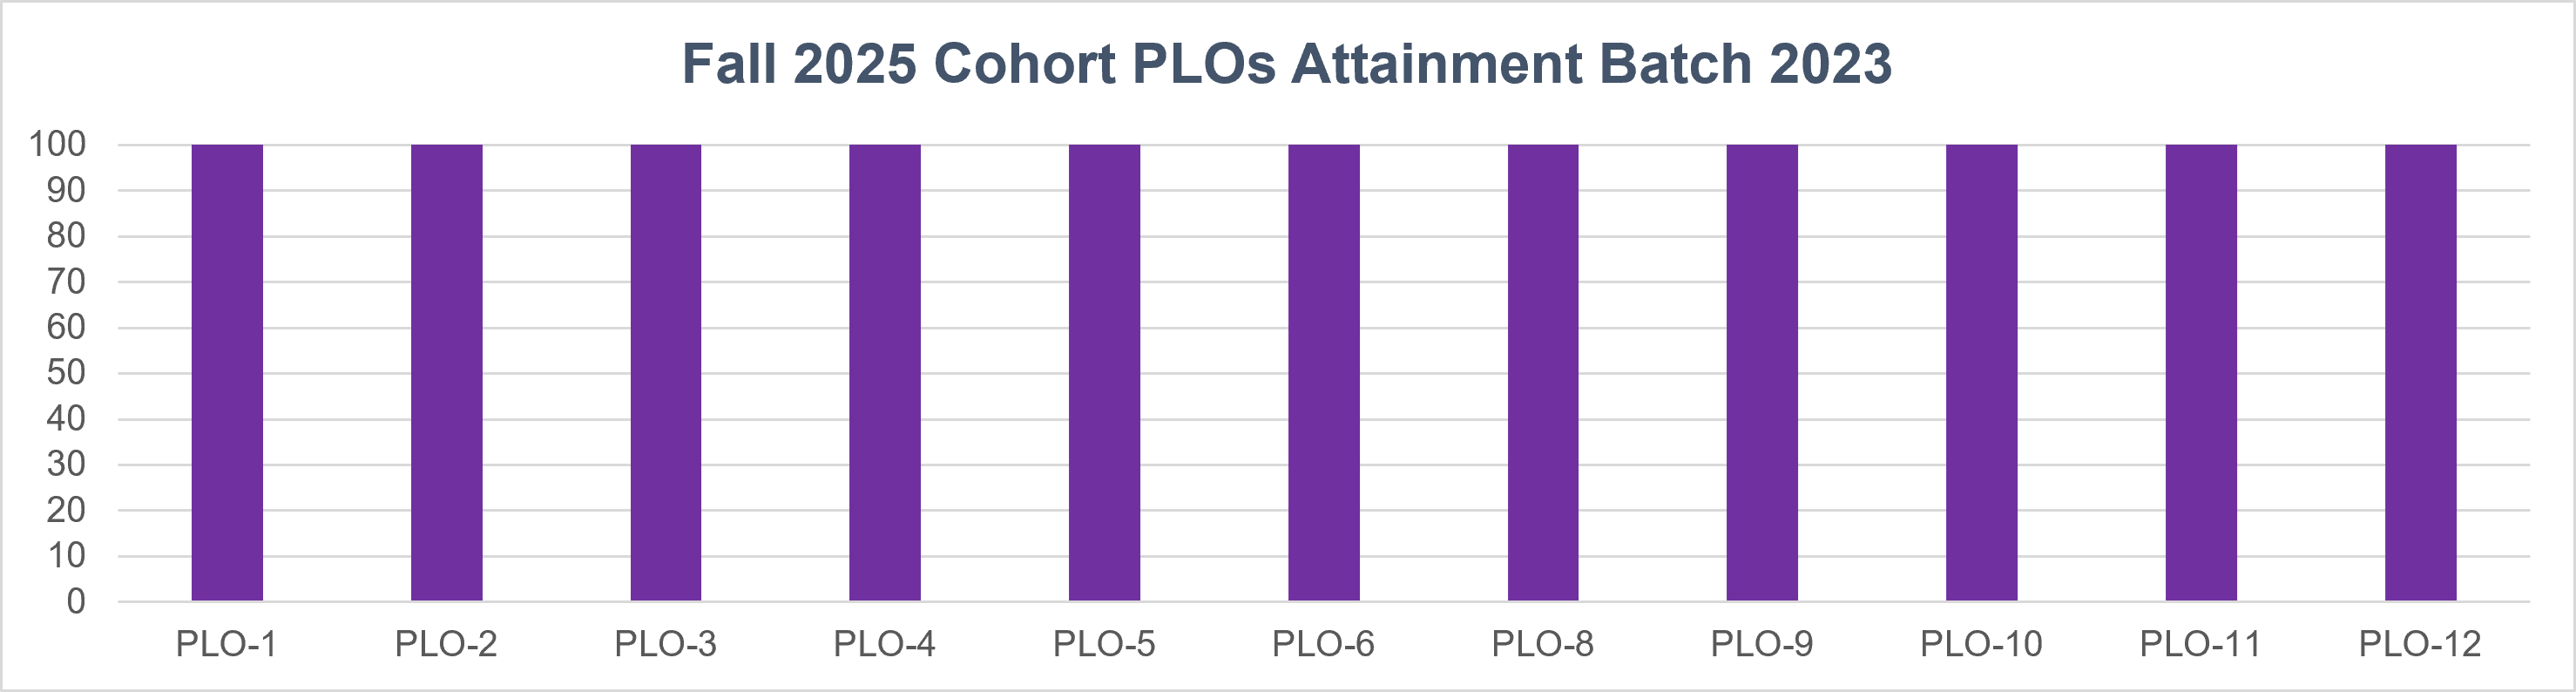
\includegraphics[width=0.98\textwidth]{images/criterion_2/media/image19.png}
\caption{2K23 Batch cohort PLO attainment against the 60\% KPI.}
\label{figure:2023 Batch cohort PLO attainment}
\end{figure}

\subsubsection{PLO Attainment at Individual Level}

Data from each course is forwarded to the exam branch which maintains a compilation of all courses for a particular batch. Data for each student is being maintained for PLOs as ``Y'' for PLOs attained by student and ``N'' for those not attained. A sample chart for a student showing attainment of PLOs is shown in Table~\ref{table:Cohort CLOs Attainment for CS-251}.

\clearpage
\begin{landscape}
\begingroup\scriptsize\setlength{\tabcolsep}{2pt}
\begin{longtable}{>{\raggedright\arraybackslash}p{0.10\linewidth}
                  >{\centering\arraybackslash}p{0.07\linewidth}
                  >{\raggedright\arraybackslash}p{0.18\linewidth}
                  >{\centering\arraybackslash}p{0.042\linewidth}
                  >{\centering\arraybackslash}p{0.042\linewidth}
                  >{\centering\arraybackslash}p{0.042\linewidth}
                  >{\centering\arraybackslash}p{0.042\linewidth}
                  >{\centering\arraybackslash}p{0.042\linewidth}
                  >{\centering\arraybackslash}p{0.042\linewidth}
                  >{\centering\arraybackslash}p{0.042\linewidth}
                  >{\centering\arraybackslash}p{0.042\linewidth}
                  >{\centering\arraybackslash}p{0.042\linewidth}
                  >{\centering\arraybackslash}p{0.050\linewidth}
                  >{\centering\arraybackslash}p{0.042\linewidth}
                  >{\centering\arraybackslash}p{0.042\linewidth}}
\caption{PLOs Attainment for an Individual Student. Student Name: Muhammad Sohaib Akhtar, Registration No.: 456318 (2023 Batch)} \\
\toprule
\textbf{Semester} & \textbf{Code} & \textbf{Course Title} & \textbf{PLO-1} & \textbf{PLO-2} & \textbf{PLO-3} & \textbf{PLO-4} & \textbf{PLO-5} & \textbf{PLO-6} & \textbf{PLO-7} & \textbf{PLO-8} & \textbf{PLO-9} & \textbf{PLO-10} & \textbf{PLO-11} & \textbf{PLO-12} \\
\midrule
\endfirsthead
\multicolumn{15}{l}{\footnotesize\textit{Continued from previous page}} \\
\toprule
\textbf{Semester} & \textbf{Code} & \textbf{Course Title} & \textbf{PLO-1} & \textbf{PLO-2} & \textbf{PLO-3} & \textbf{PLO-4} & \textbf{PLO-5} & \textbf{PLO-6} & \textbf{PLO-7} & \textbf{PLO-8} & \textbf{PLO-9} & \textbf{PLO-10} & \textbf{PLO-11} & \textbf{PLO-12} \\
\midrule
\endhead
\midrule\multicolumn{15}{r}{\footnotesize\textit{Continued on next page}} \\
\endfoot
\bottomrule
\endlastfoot
\textbf{1 (Fall-2023)} & CS-110   & Fundamentals of Computer Programming & Y & & Y & & Y & & & & Y & & & \\
 & HU-107   & Pakistan Studies                    &   &   &   &   &   & Y &   & Y &   &   &   & Y \\
 & HU-110   & English                             &   &   &   &   &   &   &   &   &   & Y &   & Y \\
 & MATH-101 & Calculus \& Analytical Geometry     & Y & \cellcolor{Red!20}{N} &   &   &   &   &   &   &   &   &   &   \\
 & MATH-161 & Discrete Mathematics                & Y & Y & Y &   &   &   &   &   &   &   &   &   \\
 & OHS-101  & Occupational Health and Safety      &   &   &   &   &   & Y & Y &   &   &   &   &   \\
 & PHY-102  & Applied Physics                     & Y & Y &   &   &   &   &   &   &   &   &   &   \\
\textbf{2 (Spr.-2024)} & CS-212  & Object Oriented Programming         & Y & Y & Y &   & Y &   &   & Y &   &   &   &   \\
 & EE-122   & Computer Architecture and Logic Design & Y & Y & Y & Y & Y &  &  & Y & Y &  &  &  \\
 & HU-101   & Islamic Studies                     &   &   &   &   &   & Y &   & Y &   &   &   & Y \\
 & HU-109   & Communication Skills                &   &   &   &   &   &   &   & Y &   & Y &   & Y \\
 & MATH-121 & Linear Algebra \& ODEs              & Y & Y &   &   &   &   &   &   &   &   &   &   \\
 & ME-105   & Workshop Practice                   & Y &   & Y &   &   &   &   &   & Y &   &   &   \\
 & ME-109   & Engineering Drawing                 & Y &   &   &   & Y &   &   &   &   &   &   &   \\
\textbf{3 (Fall-2024)} & CS-220  & Database Systems                     & Y &   & Y & Y & Y &   &   &   &   &   &   &   \\
 & CS-250   & Data Structures and Algorithms      & Y & Y &   &   & Y &   &   & Y & Y &   &   &   \\
 & EE-353   & Computer Networks                   & Y &   & Y & Y & Y &   &   &   &   &   &   &   \\
 & MATH-352 & Numerical Methods                   & Y & Y &   &   & Y &   &   &   &   &   &   &   \\
 & SE-200   & Software Engineering                & Y & Y & Y & Y &   &   &   &   & Y &   &   &   \\
\textbf{4 (Spr. 2025)} & CS-251  & Design \& Analysis of Algorithm      &   & Y & Y & Y &   &   &   &   &   &   &   &   \\
 & CS-330   & Operating Systems                   & Y & Y &   & Y & Y &   &   &   &   &   &   &   \\
 & HU-222   & Professional Ethics                 &   &   &   &   &   & Y &   & Y &   &   &   & Y \\
 & MATH-232 & Complex Variables and Transforms    & Y & Y & Y &   &   &   &   &   &   &   &   &   \\
 & MATH-361 & Probability \& Statistics           & Y & Y & Y &   &   &   &   &   &   &   &   &   \\
 & SE-211   & Software Design and Architecture    & Y & Y & Y & Y &   &   &   &   &   &   &   &   \\
\textbf{5 (Fall-2025)} & CS-336  & Embedded Systems                     & Y &   &   & Y & Y &   &   &   &   &   &   &   \\
 & CS-344   & Web Engineering                     & Y & Y &   & Y & Y &   &   &   & Y &   &   &   \\
 & HU-212   & Technical \& Business Writing       &   &   &   &   &   & Y &   &   &   & Y &   & Y \\
 & MGT-121  & Introduction To Management          &   & Y &   &   &   &   &   &   &   & Y & Y & Y \\
 & SE-314   & Software Construction               & Y & Y & Y &   & Y &   &   &   &   &   &   &   \\
 & SE-315   & Cloud Computing                     & Y & Y &   & Y & Y &   &   &   &   &   &   &   \\
\textbf{6 (Spr.-2026)} & CS-261  & Human Computer Interaction & \multicolumn{12}{l}{\textit{Spring 2026 semester in progress}} \\
 & SE-320   & Formal Methods                      & \multicolumn{12}{l}{} \\
 & SE-430   & Software Project Management         & \multicolumn{12}{l}{} \\
 & CS-471   & Machine Learning                    & \multicolumn{12}{l}{} \\
 & SE-321   & Software Quality Engineering        & \multicolumn{12}{l}{} \\
 & MGT-271  & Entrepreneurship                    & \multicolumn{12}{l}{} \\
\end{longtable}
\endgroup
\end{landscape}

%-----------------------------------------------------------------------
\hypertarget{sec:representative-course}{%
\subsection{Representative Course Result for Attainment of CLOs and PLOs}\label{sec:representative-course}}

A representative course CS-251 Design and Analysis of Algorithms, taken by 2024 batch as a core course in Spring 2026 semester is presented here to show the entire process of assessment at course level and calculations of results for attainment of CLOs as well as the PLOs. The CLO and PLO attainment report is given in Annexure~\ref{Sample CLO Attainment Report} and Annexure~\ref{Sample PLO Attainment Report}. The results for the cohort are tabulated in Table~\ref{table:Cohort CLOs Attainment for CS-251} for CLOs attainment and in Table~\ref{table:Cohort PLOs Attainment for CS-251} for PLOs attainment. Out of 45 students the percentage attainment for CLO-1, CLO-2 and CLO-3 were recorded as $91.11\%$, $91.11\%$ and $80$, respectively for the course. Figure~\ref{figure:Cohort CLO-PLO attainment Histogram} shows percent attainment of CLOs and PLOs for the entire course. The course was reviewed by the LQEC and according to OBE framework manual, attainment of all the CLOs is well above the set cohort KPI of 60\% depicting none of the corrective actions to be undertaken.

\begin{table}[H]
\centering
\caption{Cohort CLOs Attainment for CS-251 Design \& Analysis of Algorithms}
\footnotesize
\begin{tabular}{>{\raggedright\arraybackslash}p{0.50\textwidth}
                >{\centering\arraybackslash}p{0.12\textwidth}
                >{\centering\arraybackslash}p{0.12\textwidth}
                >{\centering\arraybackslash}p{0.12\textwidth}}
\toprule
\multicolumn{4}{l}{\textbf{Cohort KPI for CQI = 60\% Students Pass CLO (CLO $\geq$ 50\%)}} \\
\midrule
 & \textbf{CLO-1} & \textbf{CLO-2} & \textbf{CLO-3} \\
Total Students Attaining CLO & 41/45 & 41/45 & 36/45 \\
Percentage Students Attaining CLO & 91.11\% & 91.11\% & 80\% \\
CLO Attainment & Yes & Yes & Yes \\
\bottomrule
\end{tabular}
\label{table:Cohort CLOs Attainment for CS-251}
\end{table}

\begin{table}[H]
\centering
\caption{Cohort PLOs Attainment for CS-251 Design \& Analysis of Algorithms}
\footnotesize
\begin{tabular}{>{\raggedright\arraybackslash}p{0.50\textwidth}
                >{\centering\arraybackslash}p{0.12\textwidth}
                >{\centering\arraybackslash}p{0.12\textwidth}
                >{\centering\arraybackslash}p{0.12\textwidth}}
\toprule
\multicolumn{4}{l}{\textbf{Cohort KPI for CQI = 60\% Students Pass PLO (PLO $\geq$ 50\%)}} \\
\midrule
 & \textbf{PLO-2} & \textbf{PLO-3} & \textbf{PLO-4} \\
Total Students Attaining PLO & 41/45 & 41/45 & 36/45 \\
\%age Students Attaining PLO & 91.11\% & 91.11\% & 80\% \\
PLO Attainment & Yes & Yes & Yes \\
\bottomrule
\end{tabular}
\label{table:Cohort PLOs Attainment for CS-251}
\end{table}

\begin{figure}[H]
\centering
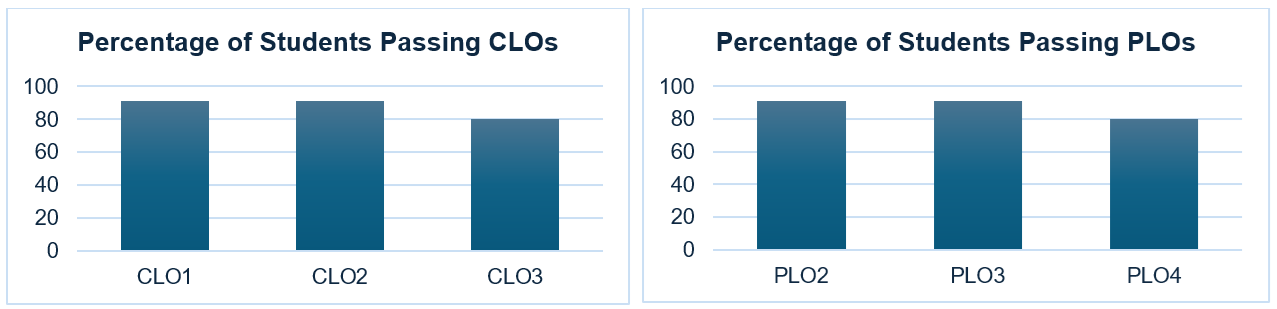
\includegraphics[width=0.99\textwidth]{images/criterion_2/media/image22.png}
\caption{Cohort CLO \& PLO attainment for CS-251 Design and Analysis of Algorithms}
\label{figure:Cohort CLO-PLO attainment Histogram}
\end{figure}

%\begin{figure}[H]
%\centering
%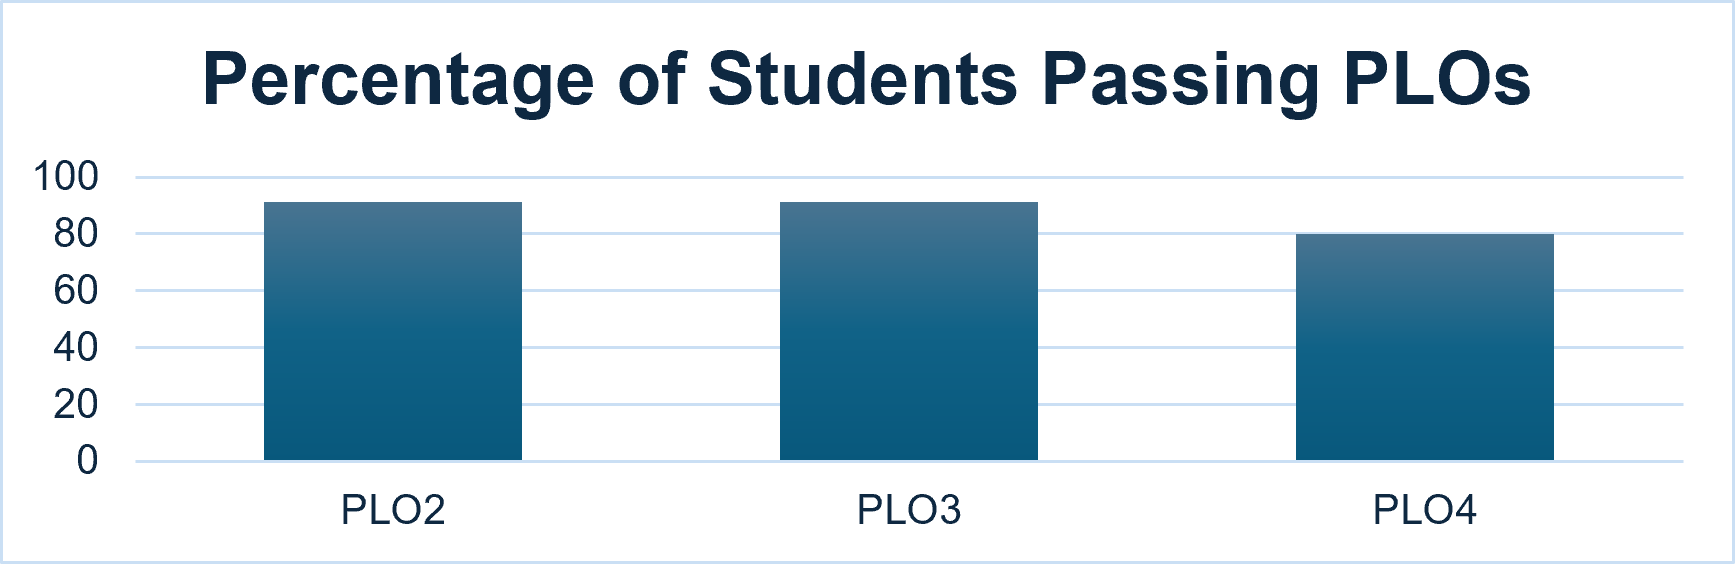
\includegraphics[width=0.86\textwidth]{images/criterion_2/media/image21.png}
%\caption{Cohort PLO attainment for CS-251 Design and Analysis of Algorithms, 2024 Batch.}
%\label{figure:Cohort PLO attainment Histogram}
%\end{figure}


%-----------------------------------------------------------------------
\hypertarget{sec:indirectassess}{%
\section{Indirect PLO Assessment}\label{sec:indirectassess}}

This method of assessment is accomplished through internship feedback and exit surveys.

\subsection{Internship Feedback}\label{sec:internshipfeedback}

Students of BESE program are required to complete their internships preferably during the summer semester. The internship feedback is obtained at the end of summer semester in their second/third year. The details of internship program are given in Chapter~\ref{criterion3}, Section~\ref{sec:4.8internship} Internship Program. The existing forms for internship feedback were revised to obtain indirect assessment of PLOs from employers of the internees. The sample internship feedback form is given in Annexure~\ref{annex:internship-feedback-form}. In the Annexure~\ref{annex:internship-feedback-analysis}, a detailed analysis of PLO attainment through internship feedback for 2K21, 2k22 and 2K23 batches is provided.

The internship feedback from employers provides indirect evidence of PLO attainment for BESE batches 2K21, 2K22, and 2K23. Overall, the results demonstrate consistently positive employer perceptions, with the majority of ratings concentrated at 4 (Very Good) and 5 (Excellent) and negligible negative ratings. Across the three batches, PLO 1 (Engineering Knowledge), PLO 11 (Project Management), and PLO 12 (Lifelong Learning) consistently emerged among the strongest attributes, indicating that graduates demonstrate sound technical foundations, effective decision-making, professional maturity, willingness to learn, and receptiveness to feedback in workplace environments.

The comparative analysis also identifies areas for continued improvement. For batches 2K21 and 2K22, PLO 2 (Problem Identification and Analysis), PLO 3 (Design and Development), and PLO 7 (Environment and Sustainability) show relatively lower proportions of Excellent ratings, although the combined Very Good and Excellent ratings remain strong. PLO 8 (Ethics) and PLO 9 (Individual and Teamwork) similarly show a strong overall performance but provide opportunities for further development. The 2K23 results, although based on interim and comparatively smaller data, show a highly positive trend, with most PLOs achieving over 90\% combined ratings of 4 and 5. Overall, the three-batch comparison indicates that the BESE program is effectively developing competencies valued by industry, while the identified areas of comparatively lower attainment provide useful input for the CQI process. The findings can therefore be used to strengthen curriculum content, practical and design-oriented activities, professional skills development, and industry exposure, particularly in complex problem-solving, system design, sustainability, and workplace professionalism.

\subsection{Exit Survey}

The exit survey seeks graduating students input on quality of education they received during their program. The purpose of this survey is to assess the perception of graduating students on achievement of PLOs. Sample of the exit survey form is given in Annexure~\ref{annex:graduate-exit-survey-form}.

The Graduate Exit Survey provides indirect evidence of PLO attainment through graduating students’ self-assessment on a 5-point Likert scale. The results for batches 2K20, 2K21, and 2K22 demonstrate consistently positive attainment across all 12 PLOs, with mean scores generally close to or above 4.0. The 2K20 batch showed a particularly stable performance, with students expressing strong confidence in lifelong learning, communication, and professional competencies. The 2K21 batch similarly demonstrated strong performance, particularly in ethics, teamwork, communication, and engineering and societal considerations.

The 2K22 batch maintained a positive overall profile, with teamwork (PLO 9), lifelong learning (PLO 12), and communication (PLO 10) emerging as the strongest areas. Across the batches, some variation was observed in students’ perceptions of engineering knowledge, problem analysis, design and development, modern tool usage, and professional ethics, providing useful areas for further attention. In particular, the relatively lower scores for PLO 8 and PLO 5 in 2K22 indicate opportunities to further strengthen ethical responsibility, accountability, and hands-on familiarity with evolving industry tools.

Overall, the exit survey results indicate that graduates perceive themselves as well prepared in both technical and professional competencies, with strong capabilities in communication, teamwork, ethical/professional conduct, management, and lifelong learning. The identified areas of relatively lower attainment are used as input to the CQI process to further enhance curriculum content, practical exposure, assessment strategies, and professional development activities. The detailed analysis of graduate exit survey is provided in Annexure~\ref{annex:graduate-exit-survey-analysis}. 

%-----------------------------------------------------------------------
\hypertarget{sec:application}{%
\section{Application of Assessment Results for Improvement of Program}\label{sec:application}}

LQEC evaluates results of the course in consultation with the concerned faculty and HoD for any recommended improvements. If some deficiency is identified through CQI, the corrective action process is invoked by the LQEC. The process for corrective action identifies the nature of problems that may be improved through review process as described in Section~\ref{sec:cqiplos}. If the weakness is related to achievement of CLOs and/or PLOs through coursework, the revision of curriculum or other corrective actions are recommended. The possible corrective actions may be, the revision of curriculum, redefining of CLOs, revision of CLOs to PLOs mapping, the assessment methods, instruction methodology, or mentoring/training of faculty.

\hypertarget{sec:cqiclos}{%
\subsection{Review and Corrective Action Process for Course (CLOs)}\label{sec:cqiclos}}

The CQI process for CLOs at SEECS is a robust, institutionalized mechanism designed to ensure that academic offerings remain rigorous, current, and tightly aligned with PLOs. Rather than being isolated or ad-hoc, CQI operates through a well-defined institutional lifecycle that guarantees traceability, formal governance review, and systematic monitoring. Figure~\ref{CLo-CQI} shows the CQI process of CLOs.

\begin{figure}[H]
\centering
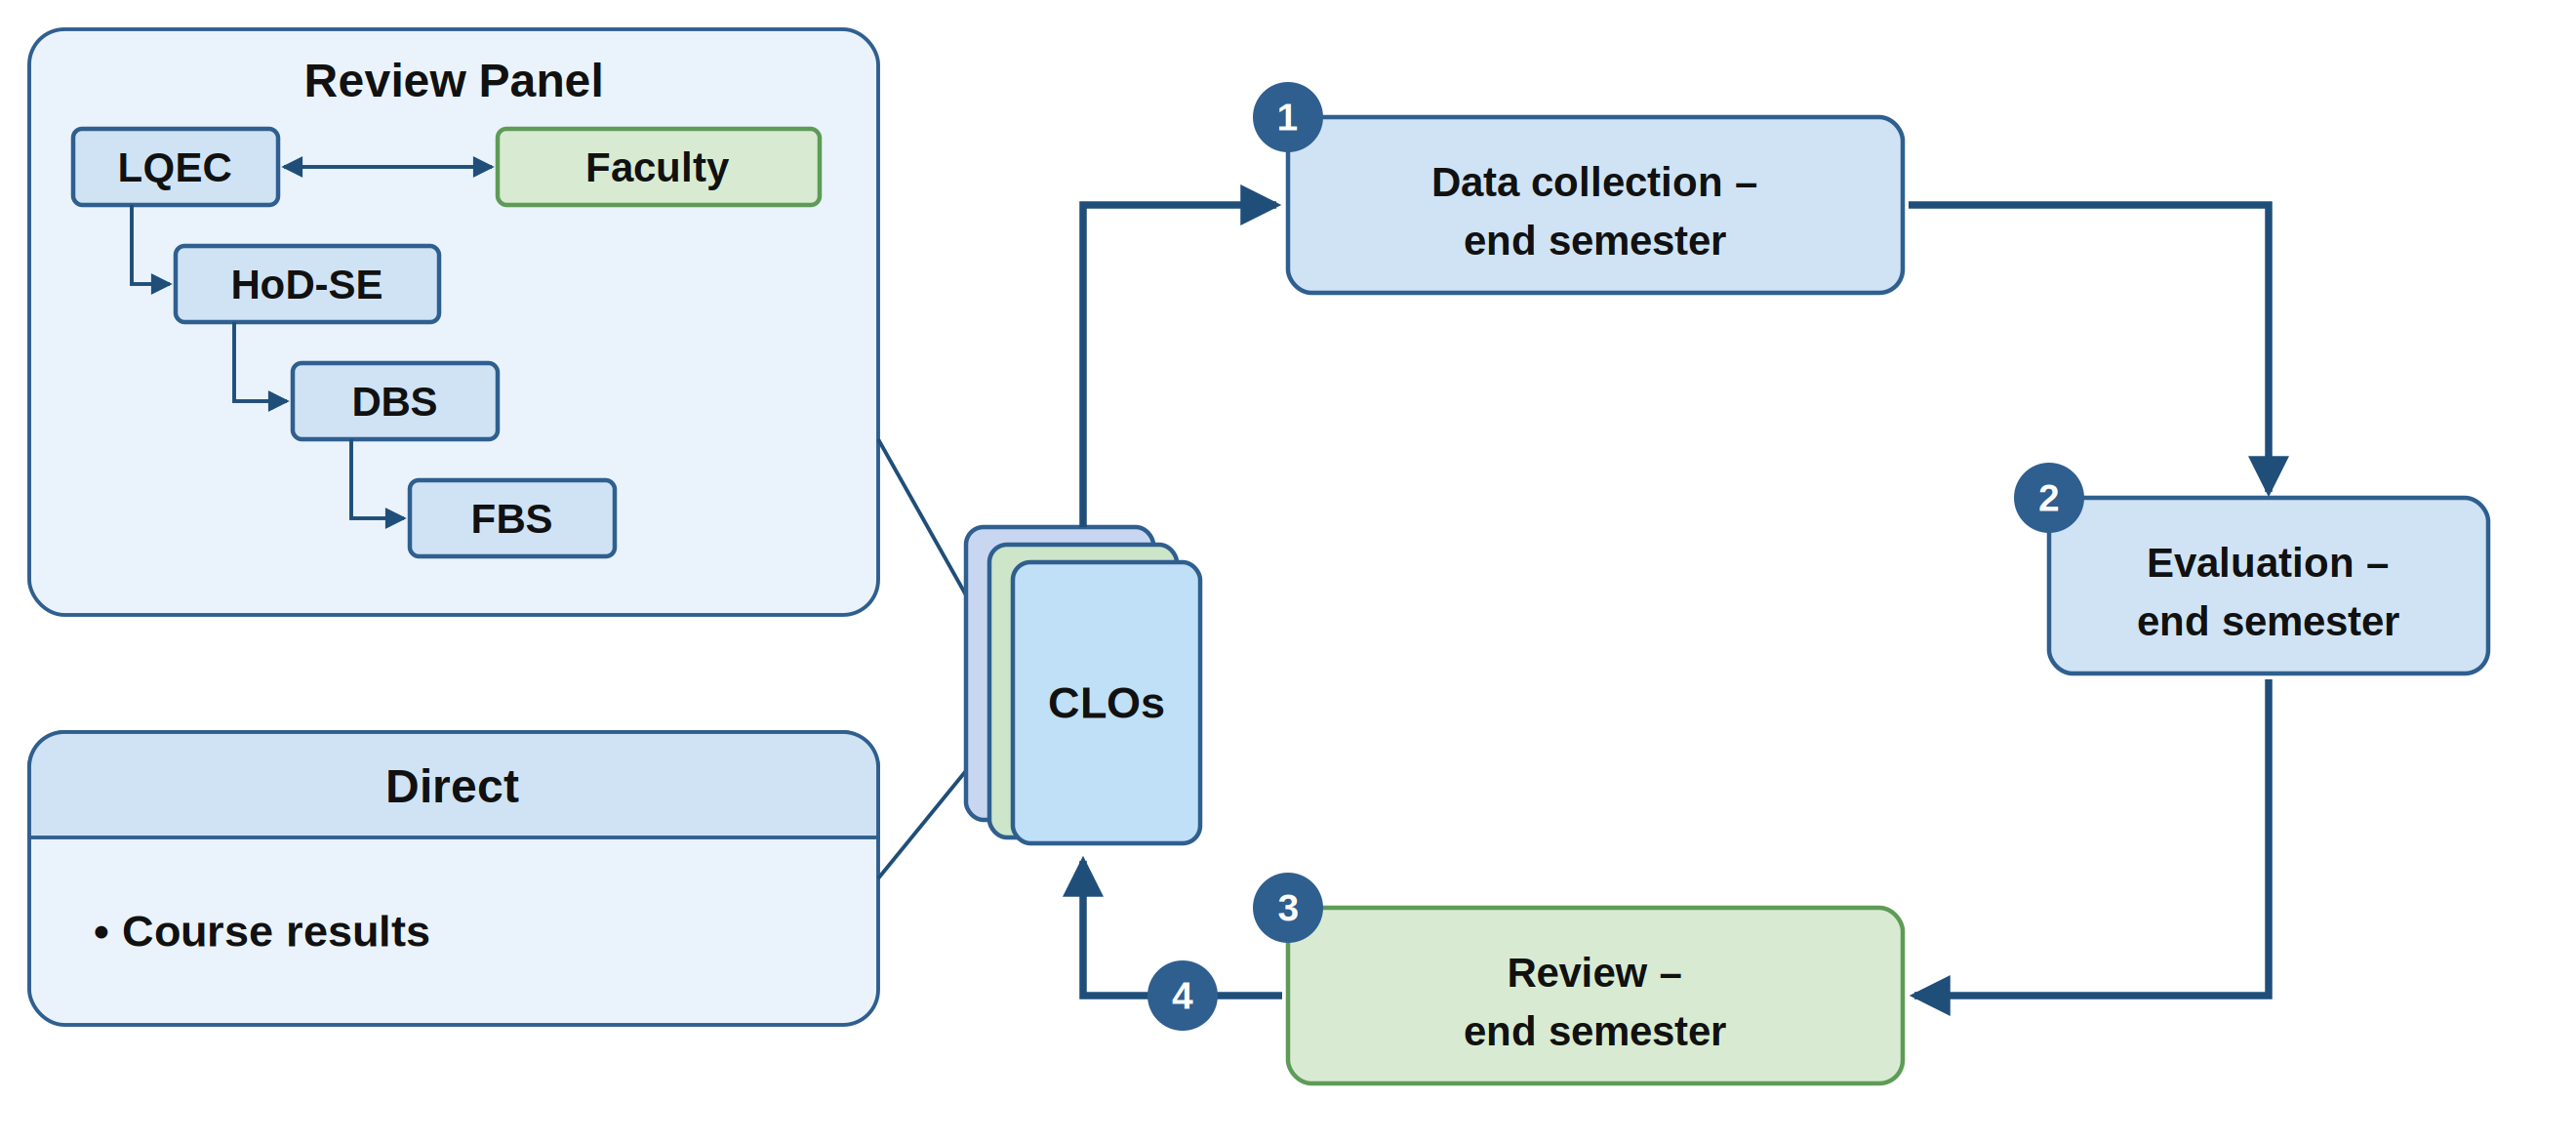
\includegraphics[width=0.9\textwidth]{images/front_matter/media/image-18.png}
\caption{Overview of the Processes Involved for Attainment and Review of CLOs.}
\label{CLo-CQI}
\end{figure}

The process universally begins with a formal identification phase, where HoD, Knowledge Group Heads (KGHs), or instructors recognize curricular deficiencies, such as misaligned CLOs, inappropriate Bloom's Taxonomy levels, outdated content, or pedagogical inconsistencies across different sections. Once an issue is identified, it is never addressed informally. Instead, it triggers a structured CQI and deliberation phase. The relevant Knowledge Group convenes to analyze the pedagogical gaps, redefine course scopes, rationalize CLO statements, and recalibrate BT levels to meet established educational benchmarks.

To demonstrate strict institutional rigor, all findings, justifications, and proposed remedies are formally captured using the Corrective Action Form (CAF). The sample corrective action form is provided in Annexure~\ref{annex:caf}. This document acts as an audit trail detailing the precise nature of the problem, the assessment of the issue, and the suggested corrective actions. Following documentation, the proposed changes cannot be implemented unilaterally. They must navigate a formal multi-tier governance structure for institutional approval. Proposed course outlines, revised CLO mappings, and curriculum updates are presented to higher academic forums such as the DBS for rigorous peer review and formal approval. Furthermore, mandatory institutional sign-offs from the LQEC, the UG Program Coordinator, and the Head of the Department validate the process before adoption. Once approved, the changes are strictly implemented in the subsequent semester, with LQEC actively monitoring execution to ensure consistent course delivery, proper assessment alignment, and improved outcome attainment. To see this institutionalized CQI process rigorously followed in practice, the curriculum review and modification for CS-212 Object-Oriented Programming (OOP) serves as a clear exemplar. The issue was formally flagged on January 31, 2024, when the Programming Core Knowledge Group identified the need to rationalize CLOs and unify programming language content across all sections of CS-212 to maintain a consistent standard of student expertise. To conduct the CQI, the Knowledge Group convened to evaluate the course structure, determining that the course would emphasize abstract OOP concepts reinforced through practical implementation in Java as a pure object-oriented language. They comprehensively updated the CLO statements, re-sequenced them, and aligned them with appropriate Bloom's Taxonomy levels and PLOs, such as upgrading CLO 2 to focus on evaluating complex programming problems at the C-5 level. This entire corrective plan was rigorously documented on an official Corrective Action Form (given in Annexure~\ref{annex:caf-oop}). Providing absolute institutional transparency and adherence to governance, the LQEC formally presented the updated course outline and revised CLOs to the DBS during its meeting on February 2, 2024 (given in Annexure~\ref{annex:dbs-mom}). The DBS formally approved the curriculum changes. The revised framework complete with updated CLOs, mapped teaching methods, and week-by-week implementation schedules, was subsequently deployed for institutional implementation starting from the Spring 2024 semester, proving that every phase of curriculum enhancement is meticulously recorded, governed, and enforced. 

\hypertarget{sec:cqiplos}{%
\subsection{Review and Corrective Action Process for PLOs}\label{sec:cqiplos}}

Monitoring the progress of individual PLOs is an iterative process assessed directly through curriculum. The data is collected, reviewed, and evaluated at the end of each academic semester where the PLO KPIs at cohort and individual level must be met. The LQEC, under the supervision of the HoD, is responsible for monitoring cohort PLO KPI and individual students' PLO attainment. 

\subsubsection{Corrective Action Process at the Cohort Level for PLOs}
In the past 2 years, a formal invocation of corrective actions at the cohort level for PLOs has not been necessary. This sustained compliance is attributed to the consistent and successful fulfillment of established KPIs across graduating cohorts, where at least 60\% of students have continuously met the requisite 50\% threshold of overall PLO attainment, alongside meeting benchmark scores in graduate exit and internship surveys.

\begin{figure}[H]
\centering
\includegraphics[width=0.9\textwidth]{images/front_matter/media/image17.png}
\caption{Review of PLOs at Cohort Level \& Respective Corrective Actions}
\label{PLO-CQI-cohort-level}
\end{figure}

Notwithstanding these consistent outcomes, a structured CQI mechanism remains fully institutionalized under the department's OBE framework to address any potential shortfalls. Figure~\ref{PLO-CQI-cohort-level} shows the review process of PLOs at cohort level. If cohort-level PLO KPIs are not met or if critical observations arise from PEC visits, IAB meetings, or internal reviews, the LQEC initiates a formal review. Based on the identified root causes, available corrective actions range from reviewing and revising teaching and learning processes, assessment methods, and CLO-PLO mappings, to updating course contents, improving laboratory and infrastructure facilities, adjusting PLO statements or KPIs, and conducting targeted faculty trainings. Final approval for such programmatic changes rests with the FBS.

\subsubsection{Corrective Action Process at the Individual Level for PLOs}
At the individual level, students’ attainment of the PLOs is monitored throughout the degree program using assessment results. The LQEC, under the supervision of the HoD and in coordination with the Academic Coordination Branch (ACB), reviews individual PLO attainment at the end of each semester to identify students who have not achieved the required 50\% attainment benchmark for any PLO. A three-stage corrective action process is followed to support students in addressing identified deficiencies as shown in Figure~\ref{fig:individual level}.

\begin{figure}[H]
\centering
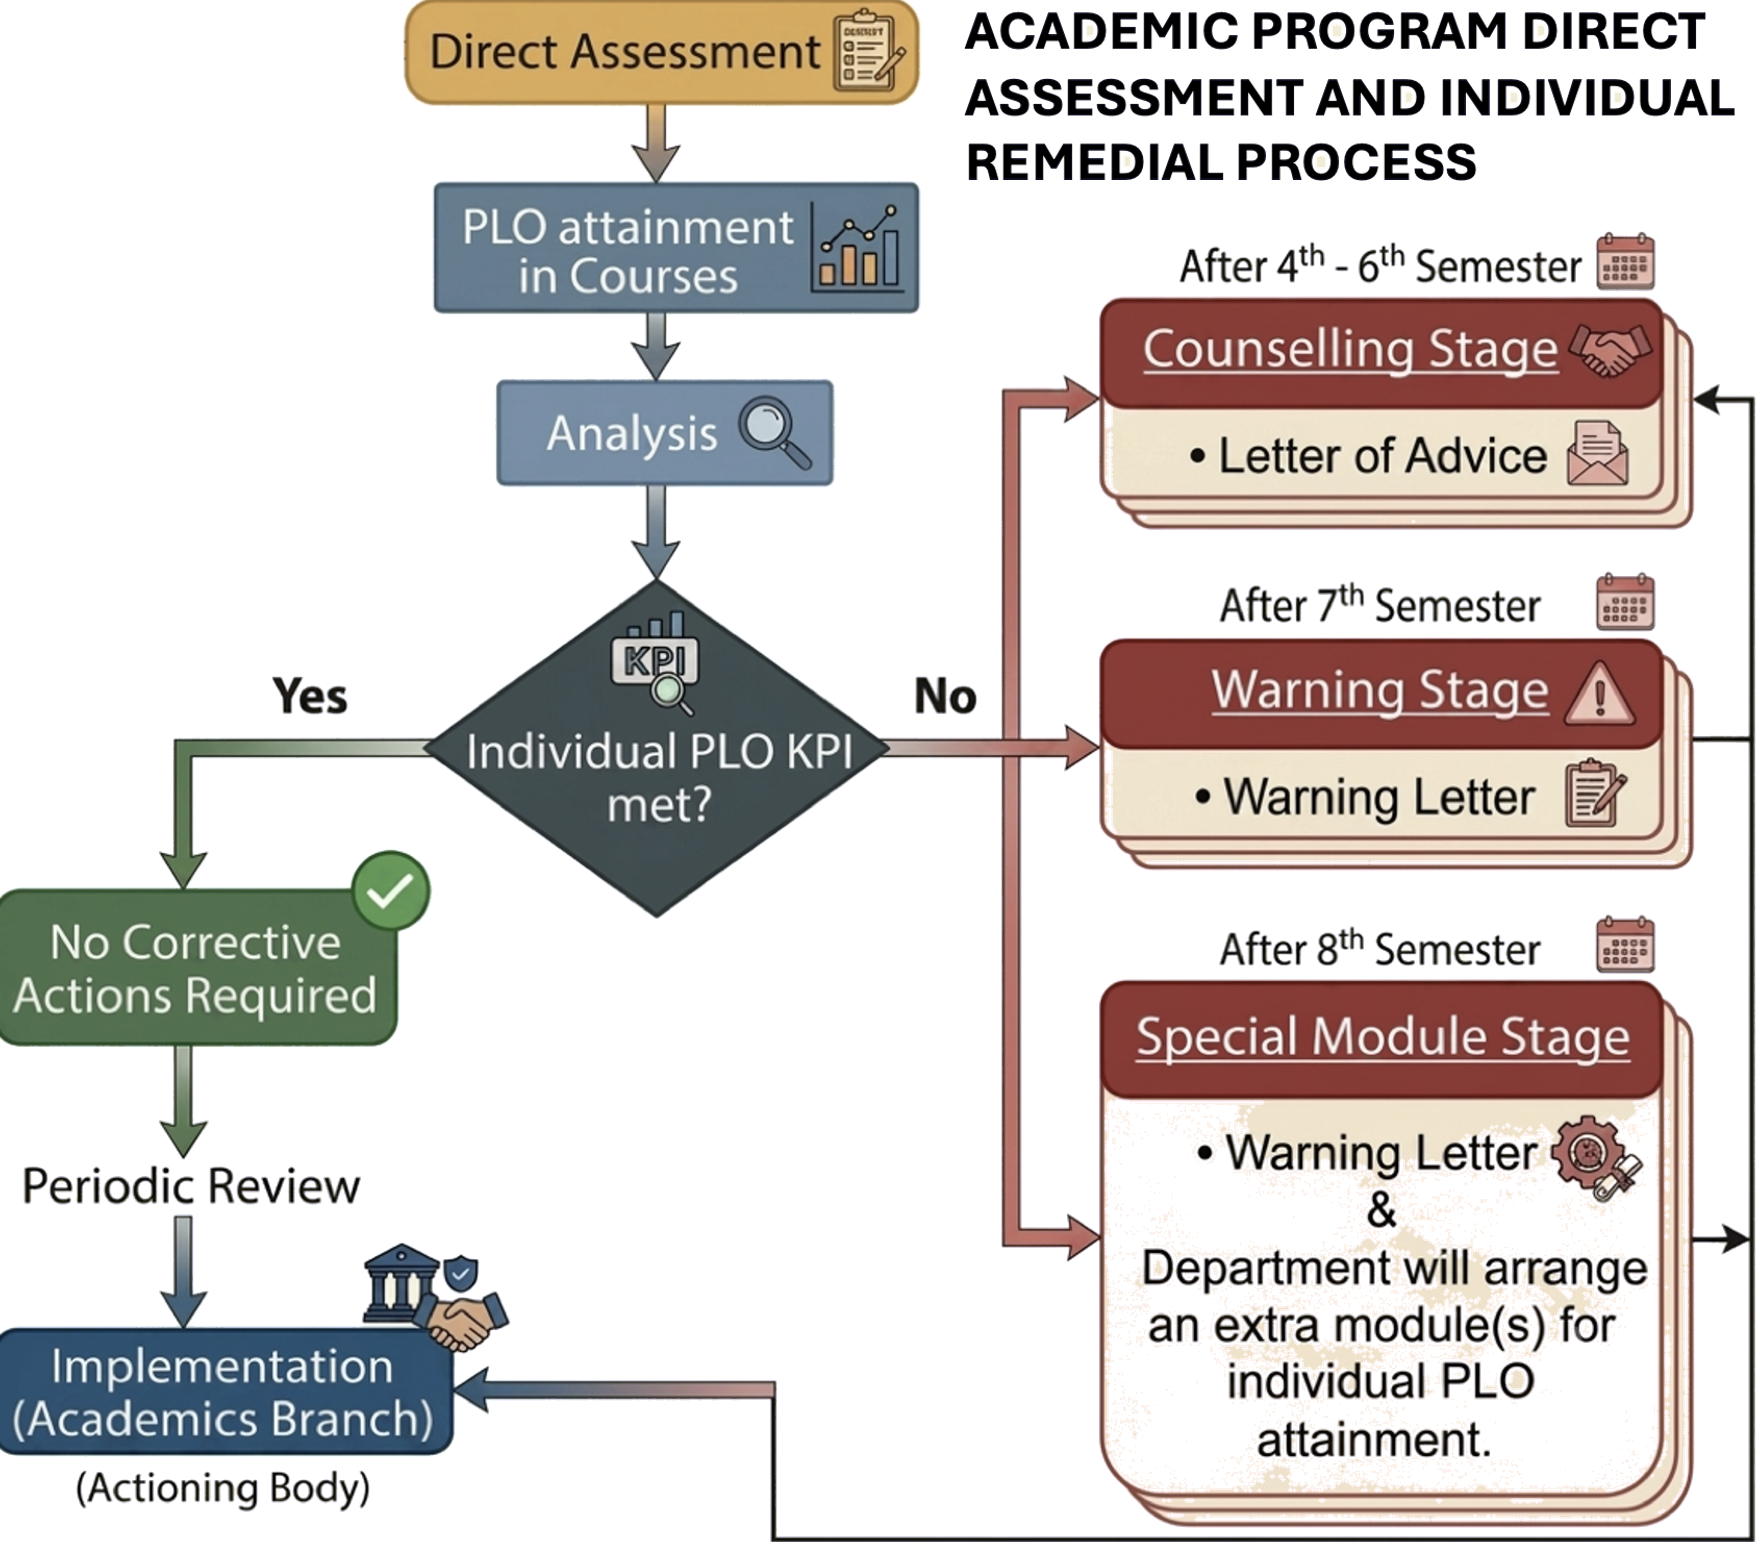
\includegraphics[width=0.7\textwidth]{images/front_matter/media/image-16.png}
\caption{Review of PLOs at Individual Level \& Corrective Actions}
\label{fig:individual level}
\end{figure}

\begin{enumerate}
\item \textbf{Counseling Stage (4\textsuperscript{th} -- 6\textsuperscript{th} Semester)}

At the end of each semester, the LQEC identifies students who have not met the required PLO attainment benchmark. Academic advisors or UG coordinators counsel these students and guide them on addressing the identified deficiencies through relevant courses and assessments in subsequent semesters. Where necessary, an advisory letter is issued to formally communicate the concern and recommended actions. A template counseling form is provided in Annexure~\ref{annex:counselling-form}.

\item \textbf{Warning Stage (7\textsuperscript{th} Semester)}

If a student continues to fall below the 50\% attainment benchmark for any PLO by the end of the 7\textsuperscript{th} semester, a formal warning letter is issued. The department reviews the deficient PLOs and, where the relevant outcome is not adequately addressed through coursework in the 8\textsuperscript{th} semester, arranges additional learning and assessment activities to help the student demonstrate the required attainment. A template warning letter is provided in Annexure~\ref{annex:warning-letter}. 

\item \textbf{Special Modules and Recovery of PLO Deficiencies}

Students who remain deficient in any PLO by the 8\textsuperscript{th} semester, or after completing their coursework, are required to undertake additional assessment activities designed to address the specific deficiency. These may include assignments, projects, case studies, or other relevant assessment tasks. Such activities may also be arranged during the summer semester, where required, to provide students with an opportunity to demonstrate the attainment of the deficient PLOs. The marks obtained through these additional assessments are used exclusively to determine PLO attainment and do not contribute to course grades.

\item \textbf{Degree Completion Requirement}

Students must meet the prescribed PLO attainment requirements to fulfil the program’s graduation requirements. A student who remains below the required attainment benchmark for any PLO must complete the prescribed recovery process and demonstrate the required attainment before the degree can be awarded. This process ensures that individual PLO deficiencies are identified systematically, communicated to students, and addressed through appropriate counseling, warnings, and additional assessment opportunities.
\end{enumerate}

%\hypertarget{sec:individual-plo}{%
%\paragraph{Individual Student PLO Achievement and Recovery of PLOs Deficiency}\label{sec:individual-plo}}

%The PLOs attainment is accomplished through direct and indirect assessments. Details of the PLOs to be assessed are provided in Section~\ref{sec:3.1plos}. For an individual student, the attainment of PLOs is required and in case of deficiency in PLOs attainment is ensured through passing of additional assignments.

%The LQEC under supervision of HoD Software Engineering, through the academic branch SEECS, is responsible for monitoring individual students' PLOs attainment. HoD Software Engineering to ensure individual students' PLOs deficiency recovery.

%Both direct and indirect assessment of PLOs for individuals usually takes place from 4\textsuperscript{th} semester at the end of each subsequent semester where the individual must achieve defined level of PLOs attainment as per KPI. At the end of each semester from the 4\textsuperscript{th} semester onwards, the LQEC of Software Engineering department will scrutinize individual PLO attainment along with semester results. Individual failing in PLOs attainment shall be informed through student academic advisors with information to HoD. Individual students will be counseled through respective student academic advisors to recover the failed PLOs that are repeated in the upcoming courses. In case of 8\textsuperscript{th} semester or a student who has completed all coursework and still PLO deficient, a letter of warning will be given to the student, and the department will arrange extra module(s) (in the form of assignment, project, case-study etc.) for individual PLO attainment. The marks attained in such CQI assessments will only be used for the attainment of related PLO of such a student. However, these marks will not be used for the calculation of the grade of the student in the related course in which the student has failed the PLO. The degree award requirements will not be considered fulfilled until the individual student has achieved the prescribed PLO KPI. These special assignments/exams will take place during the summer semester.
\subsection{Assessment-Driven Continuous Improvement of the Program}

The Software Engineering Program at SEECS uses the results of direct and indirect assessment of PLOs as a systematic input to the CQI process. Assessment results obtained through coursework, FYDP, internship feedback, and graduate exit surveys are reviewed by the LQEC to identify areas of unsatisfactory attainment, gaps in student achievement, and opportunities for further improvement. The findings are discussed within the relevant academic bodies, and corrective or improvement measures are initiated where required.

At the course level, CLO and PLO attainment results are reviewed at the end of each semester. Where deficiencies or comparatively lower attainment are identified, the results are used to review CLO formulation, Bloom's Taxonomy levels, CLO-to-PLO mapping, course contents, teaching and learning strategies, and assessment methods. The CQI process therefore provides a mechanism for progressively improving course delivery and ensuring that assessments appropriately measure the intended learning outcomes. Course outlines are reviewed and revised where necessary, with changes made through the established academic approval process.

At the program level, cohort-level PLO attainment is analyzed to determine whether the prescribed KPIs are being achieved. The results from coursework and FYDP are considered together with indirect evidence obtained from employers through internship feedback and from graduating students through the Graduate Exit Survey. This triangulation of direct and indirect evidence enables the program to identify areas requiring further attention from both academic and professional perspectives. For example, areas showing comparatively lower attainment in problem analysis, design and development, sustainability, professional skills, or familiarity with modern tools can provide input for strengthening curriculum content, practical and design-oriented activities, professional skills development, and industry exposure.

The internship feedback provides an industry perspective on the competencies demonstrated by students in professional environments. The feedback is used to identify areas where workplace competencies can be further strengthened, particularly in complex problem-solving, system design, sustainability, teamwork, and professional conduct. Similarly, the Graduate Exit Survey provides students' perceptions of their attainment of PLOs and highlights areas that may require additional attention in curriculum content, practical exposure, assessment strategies, and professional development activities.

The assessment results are also used to monitor individual student attainment. Students who do not achieve the prescribed PLO KPI are identified through the periodic review of individual PLO attainment. Such students are counseled through their academic advisors and provided opportunities to recover deficient PLOs through subsequent coursework. Where a student remains deficient after completion of coursework, additional assignments, projects, case studies, or other assessment modules are arranged to ensure attainment of the deficient PLOs before fulfillment of degree award requirements.

The overall process establishes a closed-loop mechanism in which assessment results are collected, analyzed, reviewed, and translated into improvement actions. The effectiveness of these actions is subsequently monitored through further assessment cycles. Thus, the program's PLO attainment data, stakeholder feedback, and CQI reviews provide continuous input for the progressive improvement of curriculum mapping, course design, teaching and learning practices, assessment mechanisms, practical and design experiences, and professional development opportunities. In this manner, assessment is not limited to measuring student achievement but serves as an integral mechanism for the continued development and improvement of the BE Software Engineering Program.
%-----------------------------------------------------------------------
\hypertarget{sec:materials}{%
\section{Materials used in Demonstration for Attainment of PLOs}\label{sec:materials}}

The Software Engineering Program uses a comprehensive set of academic and assessment materials to demonstrate the achievement of PLOs. These include approved course outlines containing CLOs, PLO mappings, Bloom's Taxonomy levels, course contents, and assessment methods. CLO and PLO attainment reports generated through the Qalam OBE system and course assessment evidence such as examinations, quizzes, assignments, laboratory work, projects, presentations, and assessment rubrics are employed for this purpose.

For the Final Year Design Project (FYDP), evidence includes proposal and mid-semester defense assessments, SRS and SDS documents, project progress evaluations, final reports, final defense, oral presentations, and corresponding assessment rubrics. Individual and cohort-level PLO attainment records are also maintained to demonstrate achievement against the prescribed KPIs.

In addition to direct assessment evidence, indirect assessment materials include employer internship feedback forms and analyses, as well as Graduate Exit Survey forms and analyses. These materials collectively provide direct and indirect evidence of PLO achievement and support the review of attainment through the CQI process. The consolidated evidence is maintained through Qalam, academic records, SEECS assessment systems, and relevant SAR annexures.


\clearpage

% ============================================================
% CHAPTER 4 — Criterion 3: Curriculum and Learning Process
% Images: images/criterion_3/media/
% ============================================================
\graphicspath{{images/criterion_3/media/}}
\hypertarget{criterion3}{%
\chapter{Criterion 3: Curriculum and Learning Process}\label{criterion3}}

\begin{comment}
\newcommand{\missingcriterionthreefigure}[1]{%
  \par\smallskip
  \textcolor{red}{\textbf{[Review required: figure caption and label are missing for \texttt{#1}.]}}%
}

\begin{center}
\fcolorbox{red}{red!5}{%
\begin{minipage}{0.92\textwidth}
\textbf{Criterion 3 Evidence Completeness Review}

\textcolor{red}{\textbf{Missing annexure PDFs:}} Annex A, Annex C, Annex D, Annex E.1, Annex E.2, Annex F, Annex G, Annex N, Annex O, Annex U, Annex Y, Annex Z, Annex AD-1, Annex AD-2, and Annex AL.

\textcolor{red}{\textbf{Figure review:}} All 21 referenced image files are present. However, 13 figure environments have no caption, and all 21 figure environments have no \texttt{\string\label}. Captionless figures are marked in red at their locations below.
\end{minipage}}
\end{center}
\end{comment}

%-----------------------------------------------------------------------
\hypertarget{sec:4.1programstructure}{%
\section{Program Structure}\label{sec:4.1programstructure}}
The BESE program at SEECS is designed around the needs of its key stakeholders, including industry, students, and the university, as reflected in the program’s mission, objectives, and PLOs, which shape a curriculum mapped against the PLOs (Section~\ref{sec:3.1plos}). NUST currently offers BESE at two constituent institutes: Military College of Signals (MCS), Rawalpindi, and NUST-SEECS, H-12 Campus. MCS has offered the program for 14 years, while NUST-SEECS' version was approved in the 32nd ACM (2010), differing only in a few courses. As part of NUST's move toward curriculum unification across constituent colleges, both institutes were directed to develop a single, unified BESE curriculum aligned with national (HEC, PEC) and international (ACM/IEEE) standards. The curriculum undergoes periodic review at the Departmental Board of Studies (DBS), with recommendations forwarded to the UCRC/ACM for approval. Revisions are carried out annually to reflect HEC guidelines, international developments, and evolving local industry needs, ensuring alignment with HEC, PEC, and NUST Academic Council requirements.

NUST-SEECS follows a semester system, with the 4-year BESE program comprising 8 semesters of 18 weeks each. The overall program breakdown is given in Table~\ref{tab:bep}.

\begin{table}[H]
\centering
\footnotesize % <-- Reduces font size
\renewcommand{\arraystretch}{0.85} % <-- Tightens vertical row spacing
\caption{BESE Engineering Program}
\label{tab:bep}
\begin{tabular}{>{\raggedright\arraybackslash}p{0.50\textwidth}
                >{\raggedright\arraybackslash}p{0.32\textwidth}}
\toprule
\textbf{Duration} & 4 years \\
\midrule
\textbf{Number of Semesters} & 8 \\
\textbf{Number of Weeks per Semester} & 18 (16 for teaching, 2 for exams) \\
\textbf{Total credit hours for BESE 2021--2024 batches} & 134 + X \\
\textbf{Total credit hours for BESE 2025 \& onwards batches} & 138 + X \\
\textbf{Number of credit hours per semester} & 15--19 \\
\textbf{Engineering courses} & 30 courses, 95+ Cr Hrs \\
\textbf{Non-Engineering courses} & 19 courses, 43 Cr Hrs \\
\bottomrule
\end{tabular}
\end{table}

\hypertarget{sec:4.2curriculum}{%
\section{Program Curriculum}\label{sec:4.2curriculum}}
The BESE program's academic curriculum is designed to help all students meet the program learning outcomes (PLOs) through a balanced combination of technical and non-technical subjects, along with appropriate assessments and evaluations. A clearly defined core of essential subjects, guided by the standards set by PEC and HEC in Pakistan, supports the program's vision, mission, and PLOs. The curriculum review process is depicted in Figure ~\ref{figure:pfcr}.

\begin{figure}[H] \centering 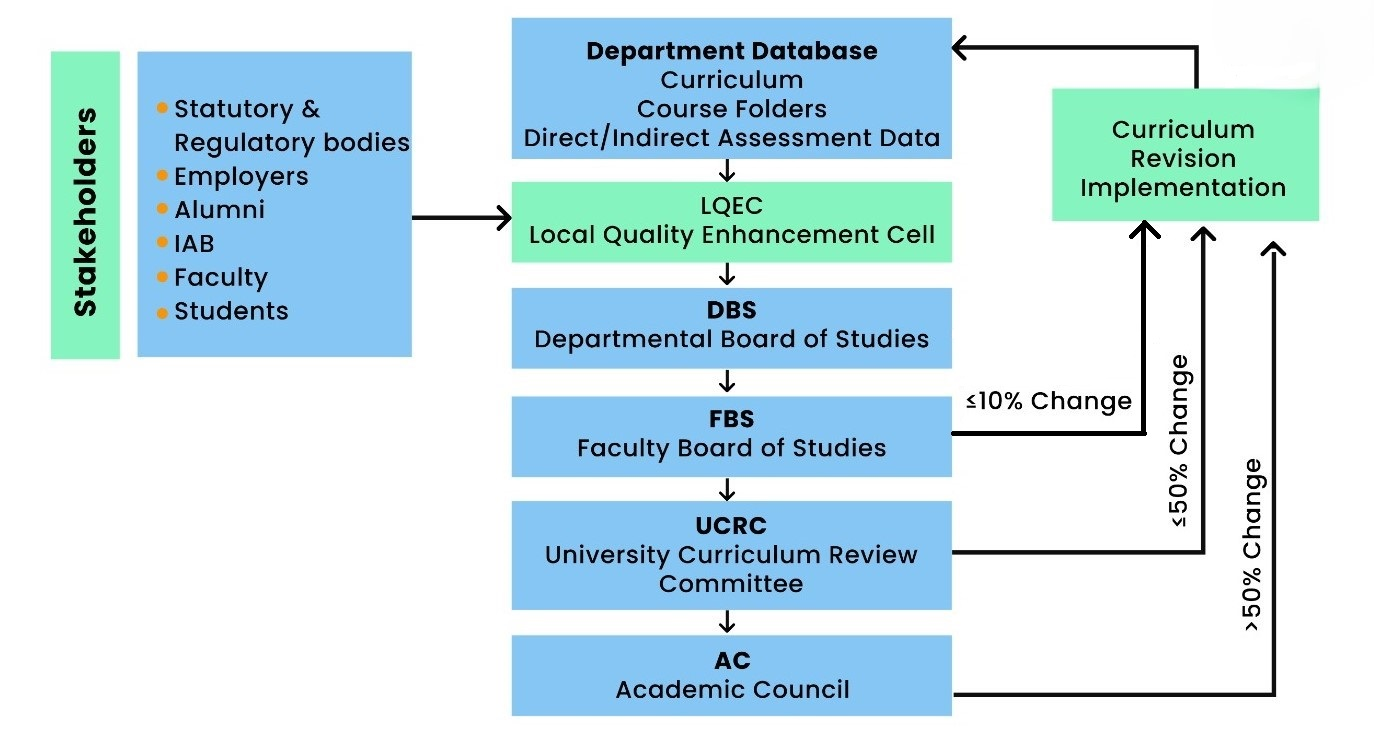
\includegraphics[width=0.92\textwidth]{images/criterion_8/media/Curr_review.jpeg} \caption{Processes for Curriculum Review} \label{figure:pfcr} \end{figure} 

The curriculum is composed of a balanced combination of engineering and non-engineering domains coupled with appropriate assessment and evaluation methods. The program curriculum involves both theory and laboratory work through all three learning domains of Bloom's Taxonomy. The cognitive, psychomotor, and affective domains cover 74\%, 15\% and 11\% of the curriculum, respectively, as shown in Figure~\ref{figure:percentage_bloom_taxonomy}.
\begin{figure}[!h]
    \centering
    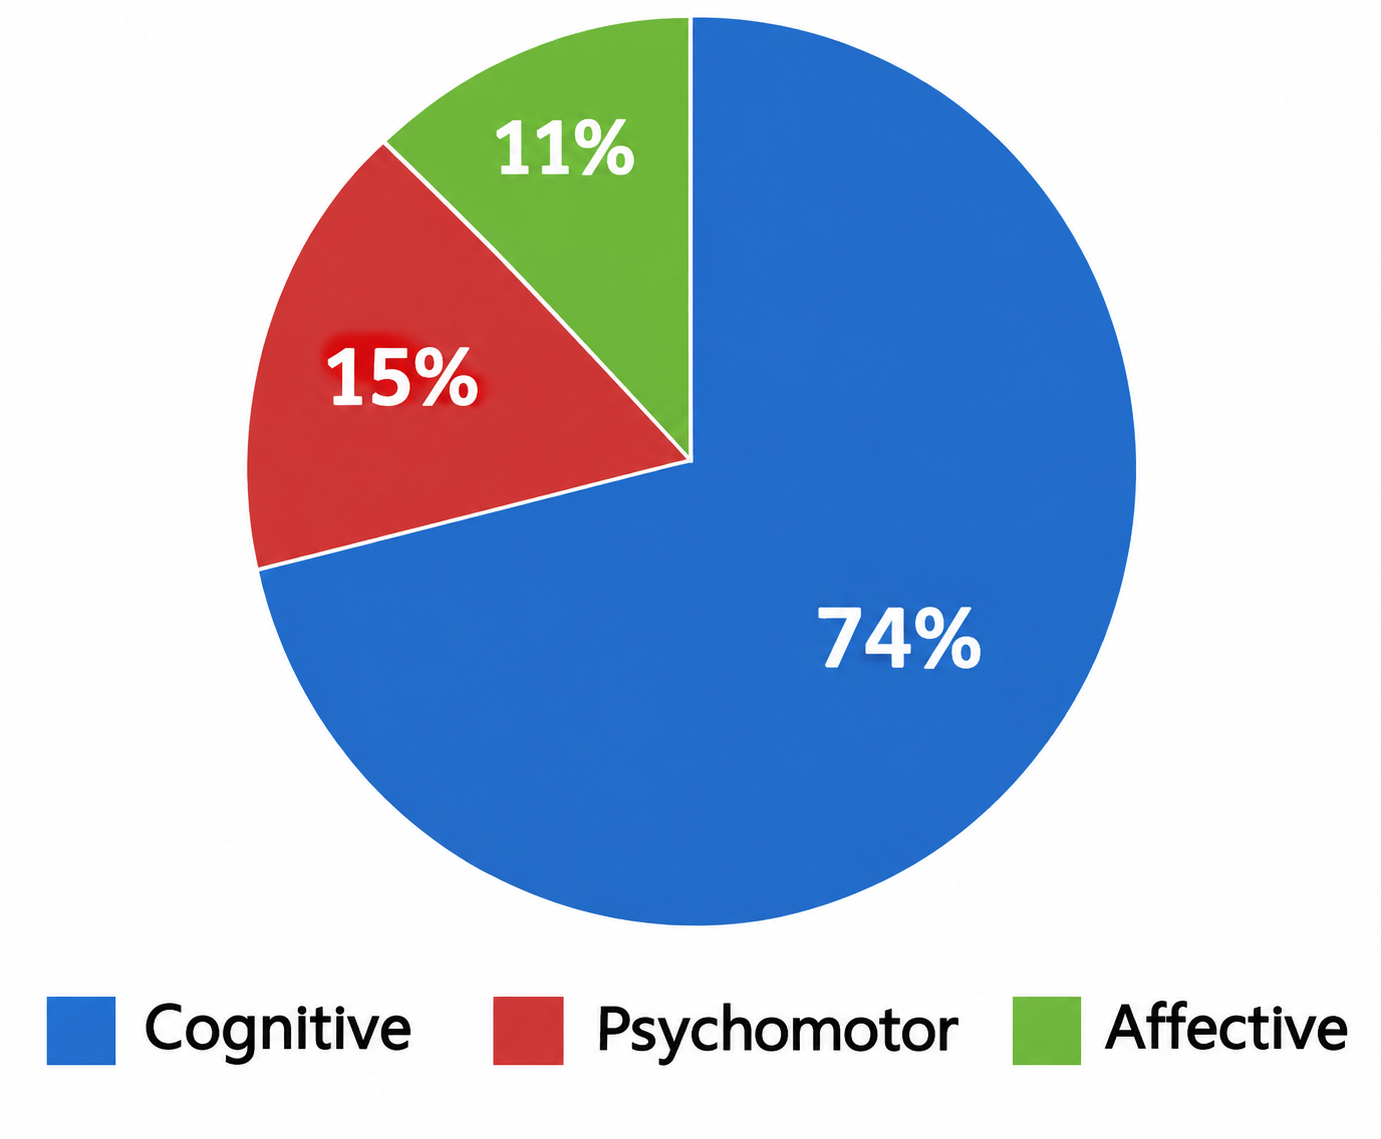
\includegraphics[width=0.50\textwidth]{images/criterion_3/media/BT-Domains.png}
    \caption{Percentage of Learning Domains of Bloom's Taxonomy}
    \label{figure:percentage_bloom_taxonomy}
\end{figure}
%\begin{comment}
%\begin{figure}[H]
%\centering
%\includegraphics[width=0.92\textwidth]{images/criterion_3/media/image10.png}
%\caption{Figure 4.2: Program Structure Outline}
%\end{figure}
%\end{comment}
The curriculum developed for BESE Program at NUST-SEECS also encompasses the national requirements based on engineering and non-engineering areas. The distribution of courses for BESE program at SEECS is shown in Annexure~\ref{app:criteria3-intake-2k25-wp30} (WP No.30-72nd  ACM-04 Sep 2025). It also presents the distribution of courses as per knowledge area in Software Engineering program at SEECS.

\begin{comment}
The SEECS program is benchmarked against international software engineering programs by comparing credit hours across engineering and non-engineering knowledge area domains. Table~\ref{tab:Comparison_of_Credits_of_SEECS_Program_with_International_Programs_in_Software_Engineering} shows the number of credits in each domain subdivided into subject areas, giving a comprehensive comparison with universities running a semester system.
The SEECS BESE program is benchmarked against international software engineering programs by comparing engineering and non-engineering credit hours across subject areas (Table~\ref{tab:Comparison_of_Credits_of_SEECS_Program_with_International_Programs_in_Software_Engineering}), showing strong alignment with universities using the semester system. This alignment is further illustrated in Figure~\ref{figure:Comparison_of_credits_of_SEECS_BESE_program_and_international_programs} through a histogram comparison of engineering and non-engineering credits.

\begin{figure}[H]
\centering
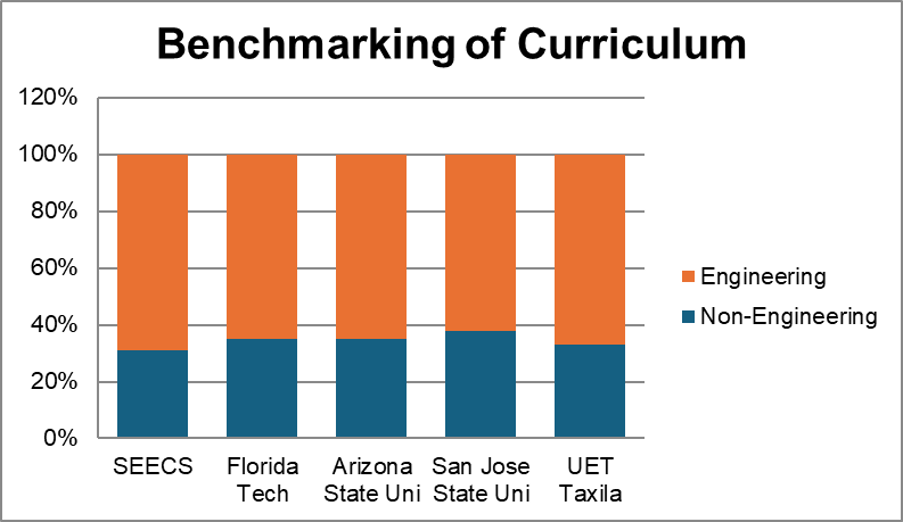
\includegraphics[width=\textwidth]{images/criterion_3/media/img_benchmarking_curriculum.png}
\caption{Comparison of credits of SEECS BESE program and international programs}
\label{figure:Comparison_of_credits_of_SEECS_BESE_program_and_international_programs}
\end{figure}

\clearpage
\begin{landscape}
\begingroup\scriptsize\setlength{\tabcolsep}{3pt}
\begin{longtable}{>{\raggedright\arraybackslash}p{0.12\linewidth}
                  >{\raggedright\arraybackslash}p{0.22\linewidth}
                  >{\centering\arraybackslash}p{0.08\linewidth}
                  >{\centering\arraybackslash}p{0.09\linewidth}
                  >{\centering\arraybackslash}p{0.10\linewidth}
                  >{\centering\arraybackslash}p{0.10\linewidth}
                  >{\centering\arraybackslash}p{0.09\linewidth}}
\caption{Comparison of Credits of SEECS Program with International Programs in Software Engineering} \\ 
\label{tab:Comparison_of_Credits_of_SEECS_Program_with_International_Programs_in_Software_Engineering}
\toprule
\textbf{Domain} & \textbf{Knowledge Area} & \textbf{SEECS} & \textbf{Florida Tech} & \textbf{Arizona State Uni} & \textbf{San Jose State Uni} & \textbf{UET Taxila} \\
\midrule
\endfirsthead
\multicolumn{7}{l}{\footnotesize\textit{Continued from previous page}} \\
\toprule
\textbf{Domain} & \textbf{Knowledge Area} & \textbf{SEECS} & \textbf{Florida Tech} & \textbf{Arizona State Uni} & \textbf{San Jose State Uni} & \textbf{UET Taxila} \\
\midrule
\endhead
\bottomrule
\endlastfoot
\textbf{Non-Engineering} & Humanities & 18 & 18 & 18 & 24 & 16 \\
 & Management Sciences & 5 & 0 & 0 & 0 & 12 \\
 & Natural Sciences & 18 & 25 & 23 & 21 & 14 \\
 & Community Service Learning & 2 & 1 & 1 & 0 & 2 \\
 & \textbf{Sub Total} & \textbf{43 (31\%)} & \textbf{44 (35\%)} & \textbf{42 (35\%)} & \textbf{45 (38\%)} & \textbf{44 (33\%)} \\
\addlinespace
\textbf{Engineering} & Computing & 7 & 10 & 15 & 13 & 25 \\
 & Engineering Foundation & 27 & 21 & 18 & 15 & 18 \\
 & Major Based Core (Breadth) & 30 & 18 & 21 & 23 & 20 \\
 & Major Based Core (Depth) & 18 & 12 & 15 & 15 & 17 \\
 & Inter-Disciplinary Eng. Breadth (Electives) & 7 & 15 & 3 & 3 & 3 \\
 & Senior Design Project & 6 & 6 & 6 & 5 & 6 \\
 & \textbf{Sub Total} & \textbf{95 (69\%)} & \textbf{82 (65\%)} & \textbf{78 (65\%)} & \textbf{75 (62\%)} & \textbf{89 (67\%)} \\
\addlinespace
\textbf{Total} & & \textbf{138} & 126 & 120 & 120 & 133 \\
\end{longtable}
\endgroup
\end{landscape}
\end{comment}

%\begin{figure}[H]
%\centering
%\includegraphics[width=0.81\textwidth]{images/criterion_3/media/image8.png}
%\caption{Figure 4.4b: Comparison of Credits (Note: Internship in summer for qualifying)}
%\end{figure}

Curriculum revision is a continuous process, and the Table~\ref{tab:Revision_of_BESE_Curriculum} shows the curriculum revision timeline since 2023.
\begin{table}[htbp]
\centering
\footnotesize % <-- Reduces font size
\renewcommand{\arraystretch}{0.85} % <-- Tightens vertical row spacing
\caption{Curriculum Revision Timeline}
\label{tab:Revision_of_BESE_Curriculum}
\begin{tabular}{c >{\raggedright\arraybackslash}p{0.36\textwidth} >{\raggedright\arraybackslash}p{0.46\textwidth}}
\toprule
\textbf{Ser\#} & \textbf{Working Paper (WP)} & \textbf{Description} \\
\midrule

1 & Curriculum (WP No.30--72\textsuperscript{nd} ACM-04 Sep 2025) 
  & Latest revision of BE Software Engg \newline 
    Applicable from BESE 2025 (intake Fall 2025) \newline 
    Annexure~\ref{app:criteria3-intake-2k25-wp30} \\ \addlinespace

2 & Curriculum (WP No.20--69\textsuperscript{th} ACM-06 Aug 2024) 
  & Revision of BE Software Engg \newline 
    Applicable from BESE 2024 (intake Fall 2024) \newline 
    Annexure~\ref{app:criteria-3_intake-2k24-wp20} \\ \addlinespace

3 & Curriculum (WP No.30--64\textsuperscript{th} ACM-23 Jan 2023) 
  & Revision of BE Software Engg \newline 
    Applicable from BESE 2019 (intake Fall 2019) \newline 
    Annexure~\ref{app:criteria-3_intake-2K19-wp30} \\

\bottomrule
\end{tabular}
\end{table}
The BESE program spans four years and is currently based primarily on the curriculum approved by PEC in 2020. WP No.30--64th ACM-23 Jan 2023 (Annexure~\ref{app:criteria-3_intake-2K19-wp30}) revised the FYDP credit distribution in the 7th and 8th semesters from 3 CHs each to 2 CHs and 4 CHs, respectively, to meet the minimum regular semester load. WP No.20--69th ACM-06 Aug 2024 (Annexure~\ref{app:criteria-3_intake-2k24-wp20}) aligned the BESE curriculum with PEC Engineering Education Guidelines for adopting HEC UEP-2023 (EC letter no. 15-54/Coord/2019/HEC/(CURR/UEP)/578, July 13, 2023), incorporating prescribed English courses, replacing Pakistan Studies with Ideology and Constitution of Pakistan, introducing Ethics for non-Muslim students, and adjusting semester-wise credit hour distribution within approved limits.

Subsequently, PEC issued latest guidelines (letter no. PEC/AD/CD/2025/03, April 10, 2025) for incorporating HEC UEP-2024, mandating compulsory courses such as Pakistan Studies, Fehm-e-Quran-I, and Fehm-e-Quran-II within the General Education/Non-Engineering domain effective Fall 2025. Accordingly, a revised BESE curriculum was proposed and approved in the 72nd ACM-04 Sep 2025 (Annexure~\ref{app:criteria3-intake-2k25-wp30}) to align with the updated PEC framework.

The department regularly obtains feedback from industry stakeholders through the Industrial Advisory Board (IAB). The feedback is reviewed by the department and considered as an important input for the continuous improvement and revision of the curriculum. Based on identified needs and emerging trends in the software engineering profession, appropriate changes are incorporated to enhance curriculum relevance, strengthen technical competencies, and address the evolving requirements of industry. The recommendations and their implementation are documented and monitored through the established academic review and approval mechanisms.

\begin{comment}
\begin{table}[htbp]
\centering
\caption{Revision of BESE Curriculum} % <--- Caption added here
\label{tab:Revision_of_BESE_Curriculum}                       % <--- Added label for referencing
\vspace{0.2cm}                                   % Adds spacing between caption and table
\begin{tabular}{|c|p{5cm}|p{7.5cm}|}
\hline
\rowcolor[gray]{0.7} 
\textbf{Ser\#} & \textbf{Working Paper (WP)} & \textbf{Description} \\ \hline

1 & Curriculum (WP No.30--72\textsuperscript{nd} ACM-04 Sep 2025) 
  & Revision of BE Software Engg \newline 
    Applicable from BESE 2025 (intake Fall 2025) \newline 
    Annex 3.1 \\ \hline

2 & Curriculum (WP No.20--69\textsuperscript{th} ACM-06 Aug 2024 ) 
  & Revision of BE Software Engg \newline 
    Applicable from BESE 2024 (intake Fall 2024) \newline 
    Annex 3.2 \\ \hline

2 & Curriculum (WP No.30--64\textsuperscript{th} ACM- 23 Jan 2023) 
  & Revision of BE Software Engg \newline 
    Applicable from BESE 2019 onward (intake Fall 2019) Annex 3.3 \\ \hline
\end{tabular}
\end{table}
\end{comment}

The revised distribution as per WP No.30-64\textsuperscript{th}th ACM-23 Jan 2023 (Annexure~\ref{app:criteria-3_intake-2K19-wp30})(BESE 2K19-2K23), and WP No. 20 -69th ACM-06 Aug 2024 (BESE-2K24) (Annexure~\ref{app:criteria-3_intake-2k24-wp20}) in accordance with PEC revised curriculum is presented in the Table~\ref{tab:BESE_Curriculum_(Applicable_on_2021–2024_Intakes)_vs._PEC_Curriculum_2020}. The proposed revisions as per WP~\#30, 72\textsuperscript{nd} ACM in accordance with UGEP and HEC guidelines are presented in Table~\ref{tab:BESE_Curriculum_Intake_2025} and Table~\ref{tab:BESE_Curriculum_Intake_2025_onward}.

\begin{landscape}
\begingroup\scriptsize\setlength{\tabcolsep}{3pt}
\begin{longtable}{>{\raggedright\arraybackslash}p{0.12\linewidth}
                  >{\raggedright\arraybackslash}p{0.11\linewidth}
                  >{\raggedright\arraybackslash}p{0.16\linewidth}
                  >{\centering\arraybackslash}p{0.07\linewidth}
                  >{\centering\arraybackslash}p{0.09\linewidth}
                  >{\centering\arraybackslash}p{0.07\linewidth}
                  >{\centering\arraybackslash}p{0.09\linewidth}
                  >{\centering\arraybackslash}p{0.07\linewidth}
                  >{\centering\arraybackslash}p{0.09\linewidth}}
\caption{BESE Curriculum (Applicable on 2019--2024 Intakes) vs.\ PEC Curriculum 2020} \\
\label{tab:BESE_Curriculum_(Applicable_on_2021–2024_Intakes)_vs._PEC_Curriculum_2020} \\
\toprule
\textbf{Domain} & \textbf{WK Category} & \textbf{Knowledge Area} & \multicolumn{2}{c}{\textbf{Core}} & \multicolumn{2}{c}{\textbf{Elective}} & \multicolumn{2}{c}{\textbf{Total}} \\
& & & \textbf{PEC} & \textbf{NUST SEECS} & \textbf{PEC} & \textbf{NUST SEECS} & \textbf{PEC} & \textbf{NUST SEECS} \\
\midrule
\endfirsthead
\multicolumn{9}{l}{\footnotesize\textit{Continued from previous page}} \\
\toprule
\textbf{Domain} & \textbf{WK Category} & \textbf{Knowledge Area} & \textbf{PEC Core} & \textbf{SEECS Core} & \textbf{PEC Elec.} & \textbf{SEECS Elec.} & \textbf{PEC Total} & \textbf{SEECS Total} \\
\midrule
\endhead
\bottomrule
\endlastfoot
\textbf{Engineering Domain} & WK-2/4/5/6 & Computing and Information Science & 6 & 7 & --- & --- & \textbf{6} & \textbf{7} \\
 & WK-3/2 & Engineering Foundation & 30 & 30 & - & --- & \textbf{30} & \textbf{30} \\
 & WK-4/2/1 & Software Engg.\ Core Breadth & 27 & 27 & - & --- & \textbf{27} & \textbf{27} \\
 & WK-5/6 & Software Engg.\ Core Depth & --- & --- & 18 & 18+X & \textbf{18} & \textbf{18+X} \\
 & WK-6/7/8 & Final Year Design Project & 6 & 6 & --- & --- & \textbf{6} & \textbf{6} \\
 & WK-3/4/2/1 & Multi-Disciplinary Engineering Electives & 1 & 1 & 6 & 6 & \textbf{7} & \textbf{7} \\
\addlinespace
\textbf{Non-Engineering Domain} & WK-7 & Humanities & 11 & 10 & --- & --- & \textbf{11} & \textbf{10} \\
 & --- & Social Sciences & --- & --- & 4 & 4 & \textbf{4} & \textbf{4} \\
 & --- & Management Sciences & --- & --- & 5 & 5 & \textbf{5} & \textbf{5} \\
 & WK-1 & Natural Sciences & 4 & 3 & - & - & \textbf{4} & \textbf{3} \\
 & WK-2 & Mathematics & 15 & 15 & - & - & \textbf{15} & \textbf{15} \\
 & WK-7 & Civic \& Community Engagement & 0 & 2 & --- & --- & \textbf{0} & \textbf{2} \\
\addlinespace
\textbf{Total} & & & & & & & \textbf{133} & \textbf{134+X} \\
\end{longtable}
\endgroup
\end{landscape}


\begin{landscape}
\begingroup\scriptsize\setlength{\tabcolsep}{3pt}
\begin{longtable}{>{\raggedright\arraybackslash}p{0.12\linewidth}
                  >{\raggedright\arraybackslash}p{0.11\linewidth}
                  >{\raggedright\arraybackslash}p{0.16\linewidth}
                  >{\centering\arraybackslash}p{0.07\linewidth}
                  >{\centering\arraybackslash}p{0.09\linewidth}
                  >{\centering\arraybackslash}p{0.07\linewidth}
                  >{\centering\arraybackslash}p{0.09\linewidth}
                  >{\centering\arraybackslash}p{0.07\linewidth}
                  >{\centering\arraybackslash}p{0.09\linewidth}}
\caption{BESE Curriculum (Intake 2025 \& Onwards) vs.\ PEC Curriculum 2020 -- Core and Elective Focused} \\
\label{tab:BESE_Curriculum_Intake_2025} \\
\toprule
\textbf{Domain} & \textbf{WK Category} & \textbf{Knowledge Area} & \multicolumn{2}{c}{\textbf{Core}} & \multicolumn{2}{c}{\textbf{Elective}} & \multicolumn{2}{c}{\textbf{Total}} \\
& & & \textbf{PEC} & \textbf{NUST SEECS} & \textbf{PEC} & \textbf{NUST SEECS} & \textbf{PEC} & \textbf{NUST SEECS} \\
\midrule
\endfirsthead
\multicolumn{9}{l}{\footnotesize\textit{Continued from previous page}} \\
\toprule
\textbf{Domain} & \textbf{WK Cat.} & \textbf{Knowledge Area} & \textbf{PEC Core} & \textbf{SEECS Core} & \textbf{PEC Elec.} & \textbf{SEECS Elec.} & \textbf{PEC Total} & \textbf{SEECS Total} \\
\midrule
\endhead
\bottomrule
\endlastfoot
\textbf{Engineering Domain} & WK-2/4/5/6 & Computing and Information Science & 6 & 7 & --- & --- & \textbf{6} & \textbf{7} \\
 & WK-3/2 & Engineering Foundation & 30 & 30 & - & --- & \textbf{30} & \textbf{30} \\
 & WK-4/2/1 & Software Engg.\ Core Breadth & 27 & 27 & - & --- & \textbf{27} & \textbf{27} \\
 & WK-5/6 & Software Engg.\ Core Depth & --- & --- & 18 & 18+X & \textbf{18} & \textbf{18+X} \\
 & WK-6/7/8 & Final Year Design Project & 6 & 6 & --- & --- & \textbf{6} & \textbf{6} \\
 & WK-3/4/2/1 & Multi-Disciplinary Engineering Electives & 1 & 1 & 6 & 6 & \textbf{7} & \textbf{7} \\
\addlinespace
\textbf{Non-Engineering Domain} & WK-7 & Humanities & 11 & 14 & --- & --- & \textbf{11} & \textbf{14} \\
 & --- & Social Sciences & --- & --- & 4 & 4 & \textbf{4} & \textbf{4} \\
 & --- & Management Sciences & --- & --- & 5 & 5 & \textbf{5} & \textbf{5} \\
 & WK-1 & Natural Sciences & 4 & 3 & - & - & \textbf{4} & \textbf{3} \\
 & WK-2 & Mathematics & 15 & 15 & - & - & \textbf{15} & \textbf{15} \\
 & WK-7 & Civic \& Community Engagement & 0 & 2 & --- & --- & \textbf{0} & \textbf{2} \\
\addlinespace
\textbf{Total} & & & & & & & \textbf{133} & \textbf{138+X} \\
\end{longtable}
\endgroup
\end{landscape}

\begin{comment}
%\end{gather}
\begin{table}[H]
\centering
\caption{BESE Curriculum (BESE 2025 \& Onwards) vs.\ PEC Curriculum}
\label{tab:BESE_Curriculum_Intake_2025_onward}
\begin{tabular}{>{\raggedright\arraybackslash}p{0.15\textwidth}
                >{\raggedright\arraybackslash}p{0.30\textwidth}
                >{\centering\arraybackslash}p{0.10\textwidth}
                >{\centering\arraybackslash}p{0.07\textwidth}
                >{\centering\arraybackslash}p{0.10\textwidth}
                >{\centering\arraybackslash}p{0.07\textwidth}}
\toprule
\multicolumn{6}{l}{\textbf{Curriculum Design (Fall 2025 and Onwards Batches)}} \\
\midrule
\textbf{Domain} & \textbf{Knowledge Area} & \multicolumn{2}{c}{\textbf{PEC Recommended}} & \multicolumn{2}{c}{\textbf{Institute's Program}} \\
& & \textbf{Total Credits} & \textbf{Overall \%} & \textbf{Total Credits} & \textbf{Overall \%} \\
\midrule
\textbf{Non-Engineering} & Humanities & 11 & \textbf{29.3\%} & 14 & \textbf{31.1\%} \\
 & Social Sciences & 4 & & 4 & \\
 & Management Sciences & 5 & & 5 & \\
 & Natural Sciences & 19 & & 18 & \\
 & Civic \& Community Engagement & --- & & 2 & \\
 & \textbf{Sub Total} & \textbf{39} & & \textbf{43} & \\
\addlinespace
\textbf{Engineering} & Computing & 6 & \textbf{70.7\%} & 7 & \textbf{68.9\%} \\
 & Engineering Foundation & 30 & & 30 & \\
 & Major Based Core (Breadth) & 27 & & 27 & \\
 & Major Based Core (Depth) & 18 & & 18+X & \\
 & Inter-Disciplinary Eng.\ Breadth (Electives) & 7 & & 7 & \\
 & Senior Design Project & 6 & & 6 & \\
 & Industrial Training (Summer) & 0 & & 0 & \\
 & \textbf{Sub Total} & \textbf{94} & & \textbf{95+X} & \\
\addlinespace
\textbf{Total} & & \textbf{133} & \textbf{100\%} & \textbf{138+X} & \textbf{100\%} \\
\bottomrule
\end{tabular}
\end{table}
\end{comment}

\begin{table}[H]
\centering
\footnotesize % <-- Reduces font size further
\renewcommand{\arraystretch}{0.85} % <-- Reduces row height/vertical padding
\caption{BESE Curriculum (BESE 2025 \& Onwards) vs.\ PEC Curriculum 2020}
\label{tab:BESE_Curriculum_Intake_2025_onward}
\begin{tabular}{>{\raggedright\arraybackslash}p{0.15\textwidth}
                >{\raggedright\arraybackslash}p{0.28\textwidth}
                >{\centering\arraybackslash}p{0.10\textwidth}
                >{\centering\arraybackslash}p{0.07\textwidth}
                >{\centering\arraybackslash}p{0.10\textwidth}
                >{\centering\arraybackslash}p{0.07\textwidth}}
\toprule
\multicolumn{6}{l}{\textbf{Curriculum Design (Fall 2025 and Onwards Batches)}} \\
\midrule
\textbf{Domain} & \textbf{Knowledge Area} & \multicolumn{2}{c}{\textbf{PEC Recommended}} & \multicolumn{2}{c}{\textbf{Institute's Program}} \\
& & \textbf{Total Credits} & \textbf{Overall \%} & \textbf{Total Credits} & \textbf{Overall \%} \\
\midrule
\textbf{Non-Engineering} & Humanities & 11 &  & 14 &  \\
 & Social Sciences & 4 & & 4 & \\
 & Management Sciences & 5 & & 5 & \\
 & Natural Sciences (including Maths) & 19 & & 18 & \\
 & Civic \& Community Engagement & --- & & 2 & \\
 & \textbf{Sub Total} & \textbf{39} & \textbf{29.3\%} & \textbf{43} & \textbf{31.1\%}\\
\addlinespace
\textbf{Engineering} & Computing & 6 &  & 7 &\\
 & Engineering Foundation & 30 & & 30 & \\
 & Major Based Core (Breadth) & 27 & & 27 & \\
 & Major Based Core (Depth) & 18 & & 18+X & \\
 & Inter-Disciplinary Eng.\ Breadth (Electives) & 7 & & 7 & \\
 & Senior Design Project & 6 & & 6 & \\
 & Industrial Training (Summer) & 0 & & 0 & \\
 & \textbf{Sub Total} & \textbf{94} & \textbf{70.7\%}& \textbf{95+X} &  \textbf{68.9\%} \\
\addlinespace
\textbf{Total} & & \textbf{133} & \textbf{100\%} & \textbf{138+X} & \textbf{100\%} \\
\bottomrule
\end{tabular}
\end{table}

For comprehensive achievement of BESE curriculum and all its related activities, well-defined time intervals are allocated, referred as “Credit-Hour.” One credit hour represents one contact hour a week in class or three contact hours a week of laboratory work per semester. 

\hypertarget{sec:4.7delivery}{%
\section{Delivery and Assessment Methods}\label{sec:4.7delivery}}

A broad range of teaching and assessment methods are incorporated into course outlines, designed to enable students to meet outcomes outlined in the CLOs. Students develop and practice skills through presentations and group-based cooperative learning. Program delivery covers the three learning domains of Bloom's Taxonomy (Figure~\ref{figure:percentage_bloom_taxonomy}) through theoretical coursework, laboratory work and FYDP addressing complex engineering problems.

\hypertarget{sec:4.2.1coursework}{%
\subsection{Course Work}\label{sec:4.2.1coursework}}

The BESE program at SEECS has a comprehensive system for planning and monitoring curriculum delivery. At the start of each semester, the program coordinator allocates courses and develops a delivery schedule (Timetable). Faculty prepares a detailed course outlines and submits to the Knowledge Group Head (KGH) for quality review and approval (vetted sample in Annexure~\ref{app:criteria-3_Course Outline with Knowledge Group Head's Signature}). CLOs remain constant unless revised through prescribed CQI process. Each CLO is mapped on a respective PLO to attribute the PLO attainment at the program level. Course outlines, CLOs, and assessment/action plans (Figure~\ref{figure:course_assessment_criteria}) are shared with students by the first week of the semester via Qalam and LMS. Both are regularly updated with relevant course content and marks obtained in assessments as the semester progresses. 

\begin{figure}[H]
\centering
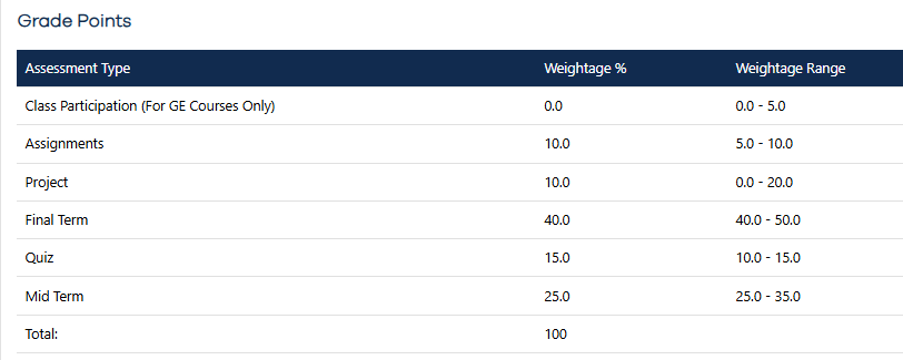
\includegraphics[width=0.97\textwidth]{images/criterion_3/media/img_course_assessment_criteria.png}
\caption{Course Assessment Criteria}
\label{figure:course_assessment_criteria}
\end{figure}

Each semester is planned to facilitate 16 weeks of teaching and 2 weeks of examination (MSE and ESE). A sample semester planner is shown in Figure~\ref{fig:planner}. Detailed data on the system of instructions and examination is given in Annexure~\ref{app:criteria-3_System of instruction and examination}. Assessment activities are distributed across the semester and their frequency is determined by the course credit hours. Generally for a course with 3 credit hours 5-6 quizzes are taken, while for a 2 credit hours course 3-4 quizzes are conducted. Similarly, 1 assignment per credit hour is taken throughout the semester. There is only one Mid Semester and one End Semester Exam per course. A semester project is usually assigned to the students in each course especially the engineering ones. For General Education courses, class participation has a mandatory weightage upto 5\%. 

All classes and labs are conducted via on-campus face-to-face mode. However, under unavoidable circumstances (i.e. lockdown etc.) the institute has online readiness capabilities via MS-Teams.

\begin{figure}[H]
\centering
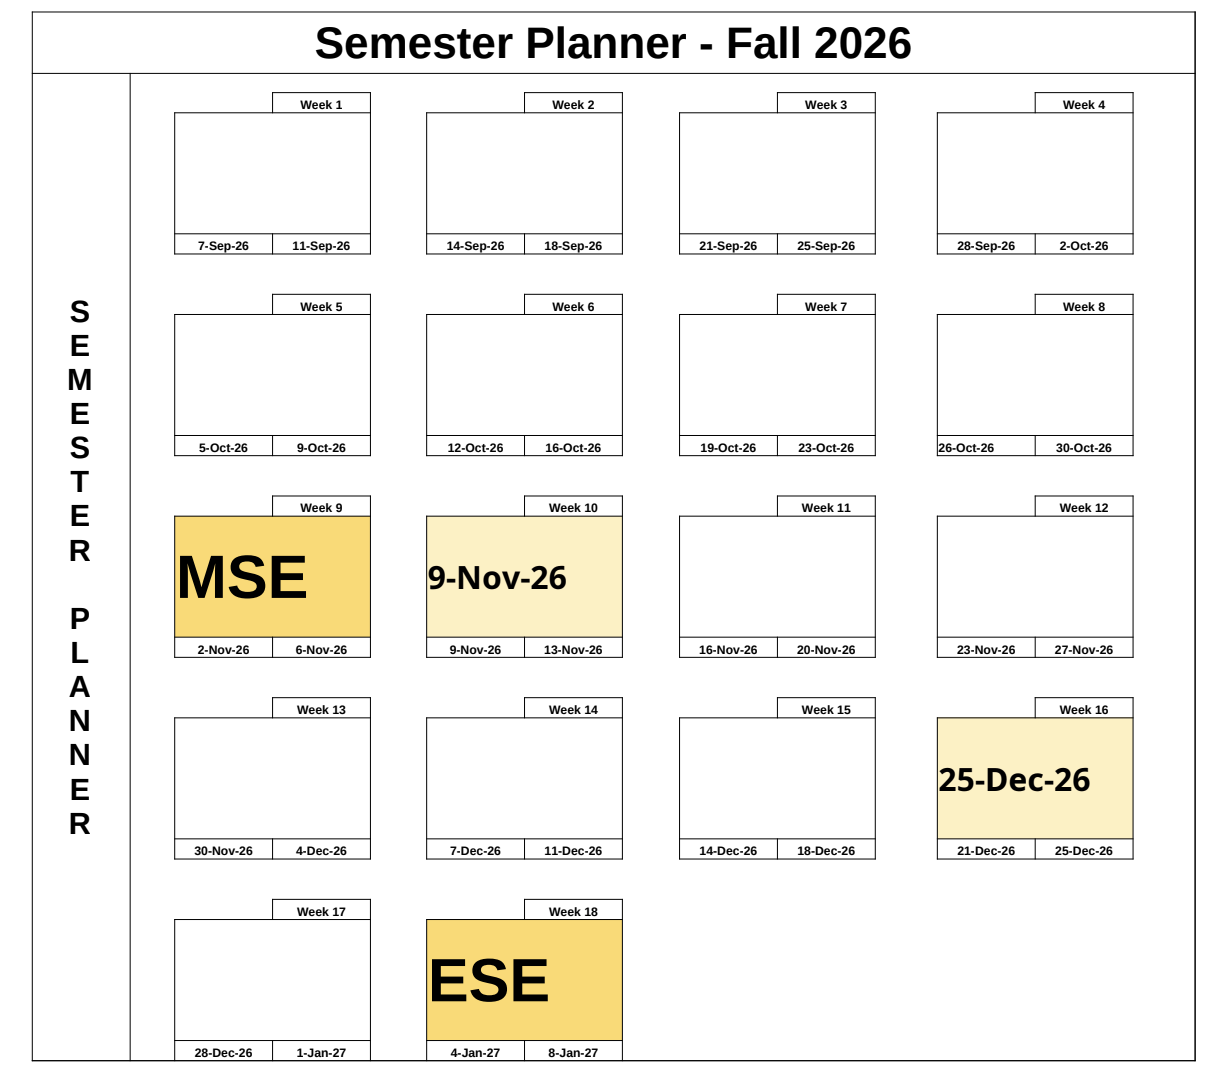
\includegraphics[width=0.97\textwidth]{images/criterion_3/media/planner.png}
\caption{Sample Semester Planner}
\label{fig:planner}
\end{figure}

%\hypertarget{sec:4.2.2coursework}{%
%\subsection{Assessment of CLOs and PLOs}\label{sec:4.2.2coursework}}

\hypertarget{sec:4.4labwork}{%
\subsection{Laboratory Work}\label{sec:4.4labwork}}

NUST-SEECS has state-of-the-art laboratories to support the Software Engineering curriculum requirements.  These laboratories are equipped with modern computing facilities and reliable networking infrastructure to support a wide range of academic and practical activities. 

\hypertarget{sec:labassessment}{%
\subsubsection{Lab Assessment}\label{sec:labassessment}}

There are at least 2 or more lab courses offered in each semester. The content of each lab from a specific course is carefully designed to meet the needs of the course and to achieve the CLOs defined for the course. The list of lab experiments for CS-368 Reinforcement Learning course is given in Table~\ref{tab:List_of_Lab_Experiments_for_CS_368_Reinforcement_Learning} as an example.

\begin{table}[H]
\centering
\small % <-- Reduces font and table size
\caption{List of Lab Experiments for CS-368 Reinforcement Learning}
\label{tab:List_of_Lab_Experiments_for_CS_368_Reinforcement_Learning}
\begin{tabular}{>{\centering\arraybackslash}p{0.12\textwidth}
                >{\raggedright\arraybackslash}p{0.62\textwidth}
                >{\centering\arraybackslash}p{0.20\textwidth}}
\toprule
\textbf{Lab No.} & \textbf{Lab Experiment} & \textbf{CLO} \\
\midrule
Lab 1  & Introduction to NumPy Library & CLO-1 / CLO-4 \\
Lab 2  & Data Visualization in Python & CLO-1 / CLO-4 \\
Lab 3  & Markov Decision Processes -- Iterative Policy Evaluation, Policy Iteration, Value Iteration & CLO-1 / CLO-4 \\
Lab 4  & Monte Carlo \& TD Learning -- Prediction [Cliff Walking \& Frozen Lake Env.] & CLO-1 / CLO-4 \\
Lab 5  & n-Step TD and TD($\lambda$) -- Prediction [Frozen Lake \& Taxi Environments] & CLO-1 / CLO-4 \\
Lab 6  & SARSA -- Control [Cart Pole \& Acrobat Environments] & CLO-1 / CLO-4 \\
Lab 7  & n-Step SARSA \& SARSA($\lambda$) -- Control [Cart Pole \& Pendulum Environments] & CLO-1 / CLO-4 \\
Lab 8  & Q-Learning \& Double Q-Learning -- Control [Mountain Car \& Lunar Lander Environments] & CLO-1 / CLO-4 \\
Lab 9  & Deep Q Networks -- I [Acrobat Environment] & CLO-1 / CLO-4 \\
Lab 10 & Deep Q Networks -- II (Stable Baselines3) [Lunar Lander \& Blackjack Environments] & CLO-1 / CLO-4 \\
Lab 11 & Advantage Actor Critic (A3C) [Bipedal Walker \& Car Racing Environments] & CLO-1 / CLO-4 \\
Lab 12 & Proximal Policy Optimization (PPO) [Pendulum \& Taxi Environments] & CLO-1 / CLO-4 \\
Lab 13 & Soft Actor Critic (SAC) [Blackjack Environment] & CLO-1 / CLO-4 \\
Lab 14 & Open Ended Lab [MuJoCo Environment] & CLO-1 / CLO-4 \\
Lab 15 & Project [Atari Environments] & CLO-2 / CLO-3 / CLO-4 \\
Lab 16 & Project [Atari Environments] & CLO-2 / CLO-3 / CLO-4 \\
\bottomrule
\end{tabular}
\end{table}

The Lab work is evaluated according to the criteria shown in Figure~\ref{figure:lab_assessment_criteria}.

\begin{figure}[H]
\centering
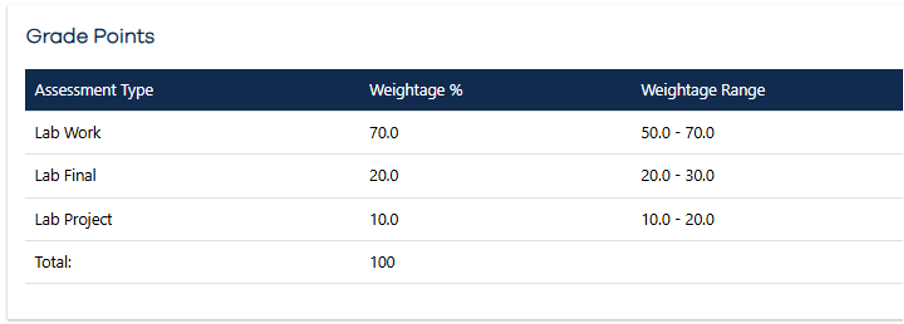
\includegraphics[width=0.97\textwidth]{images/criterion_3/media/img_lab_assessment_criteria.png}
\caption{Lab Assessment Criteria}
\label{figure:lab_assessment_criteria}
\end{figure}

Students are required to work individually or in teams of 2--3 members to accomplish practical tasks ranging from guided responses to open-ended problems. The lab folder is maintained on the LMS of NUST-SEECS. It is a comprehensive soft-copy record of all labs offered and managed by the faculty teaching the course. A sample lab manual of CS-415 Mobile Application Development (Lab~6) is given in Annexure~\ref{app:criteria-3_Sample Lab Manual}.  The lab folder in conjunction with the course folder assists academic staff in proper documentation.

\begin{comment}
\begin{table}[H]
\centering
\caption{List of Lab Experiments for CS-368 Reinforcement Learning}
\label{tab:List_of_Lab_Experiments_for_CS_368_Reinforcement_Learning}
\begin{tabular}{>{\centering\arraybackslash}p{0.10\textwidth}
                >{\raggedright\arraybackslash}p{0.74\textwidth}
                >{\centering\arraybackslash}p{0.11\textwidth}}
\toprule
\textbf{Lab No.} & \textbf{Lab Experiment} & \textbf{CLO} \\
\midrule
Lab 1  & Introduction to NumPy Library & CLO-1 / CLO-4 \\
Lab 2  & Data Visualization in Python & CLO-1 / CLO-4 \\
Lab 3  & Markov Decision Processes -- Iterative Policy Evaluation, Policy Iteration, Value Iteration & CLO-1 / CLO-4 \\
Lab 4  & Monte Carlo \& TD Learning -- Prediction [Cliff Walking \& Frozen Lake Env.] & CLO-1 / CLO-4 \\
Lab 5  & n-Step TD and TD($\lambda$) -- Prediction [Frozen Lake \& Taxi Environments] & CLO-1 / CLO-4 \\
Lab 6  & SARSA -- Control [Cart Pole \& Acrobat Environments] & CLO-1 / CLO-4 \\
Lab 7  & n-Step SARSA \& SARSA($\lambda$) -- Control [Cart Pole \& Pendulum Environments] & CLO-1 / CLO-4 \\
Lab 8  & Q-Learning \& Double Q-Learning -- Control [Mountain Car \& Lunar Lander Environments] & CLO-1 / CLO-4 \\
Lab 9  & Deep Q Networks -- I [Acrobat Environment] & CLO-1 / CLO-4 \\
Lab 10 & Deep Q Networks -- II (Stable Baselines3) [Lunar Lander \& Blackjack Environments] & CLO-1 / CLO-4 \\
Lab 11 & Advantage Actor Critic (A3C) [Bipedal Walker \& Car Racing Environments] & CLO-1 / CLO-4 \\
Lab 12 & Proximal Policy Optimization (PPO) [Pendulum \& Taxi Environments] & CLO-1 / CLO-4 \\
Lab 13 & Soft Actor Critic (SAC) [Blackjack Environment] & CLO-1 / CLO-4 \\
Lab 14 & Open Ended Lab [MuJoCo Environment] & CLO-1 / CLO-4 \\
Lab 15 & Project [Atari Environments] & CLO-2 / CLO-3 / CLO-4 \\
Lab 16 & Project [Atari Environments] & CLO-2 / CLO-3 / CLO-4 \\
\bottomrule
\end{tabular}
\end{table}
\end{comment}



\hypertarget{sec:labrubrics}{%
\subsubsection{Lab Rubrics}\label{sec:labrubrics}}

\begin{comment}
During the CQI process, the process for creating lab rubrics has been revised to address inconsistencies in rubric application across lab assessments in core depth and breadth courses. The essential requirements for the lab rubrics process are:

\begin{enumerate}[label=\alph*.]
\item Each lab for a given course must have a rubric on which the student's work can be evaluated.
\item The rubric may have one or more evaluation criteria (rubric items) to assess different outcomes associated with the lab.
\item Each rubric item must have at least three levels defined to categorize a student's work based on quality.
\item Each rubric item must have a one-to-one mapping to a CLO for the given course. Any rubric item without a corresponding CLO should be removed.
\item Each rubric item should assess the learning outcomes associated with the corresponding CLO and consequently the PLO.
\item For rubric items that use the psychomotor or affective domain, appropriate descriptors should be used and observation evidence must be maintained.
\item Once the rubric is finalized, approval is required from the faculty member and the Knowledge Group Head (KGH) to track the CQI process.
\end{enumerate}
\end{comment}

Lab works are evaluated using structured rubrics to ensure consistent  and objective assessment of students' practical performance. The attainment of CLOs and PLOs for lab/practical work is also done through these rubrics. An example of a lab rubric is given in Annexure~\ref{app:criteria-3_Lab Rubric Based Evaluation}. The lab rubrics are designed in accordance with the relevant levels of Bloom's Taxonomy, assessing students' understanding, analysis, and problem-solving skills through practical tasks. 

\hypertarget{sec:4.9othermethods}{%
\subsection{Open Ended Labs}\label{sec:4.9othermethods}}
In the courses having laboratory components in the BESE program, students are normally given an Open-Ended Lab (OEL). Students are required to understand the lab's problem and apply the studied concepts to develop a suitable solution. The implementation details are not directly provided in the lab's instructions. Students have to decide the suitable approach based on their knowledge and understanding. The OEL may involve multiple stakeholders with different or sometimes contradictory requirements. It also requires students to use the domain and foundation knowledge of the subject. The scenario does not have one fixed or well-defined solution. Multiple solutions can be valid if they properly address the given requirements and constraints. Through such OEL activities, students learn to analyze problems, identify requirements, make decisions, apply theoretical concepts, and develop practical solutions based on their knowledge and experience. An example problem given in the Reinforcement Learning Course is as follows. Detailed sample is provided in Annexure~\ref{app:criteria-3_Sample Open Ended Lab}.

\emph{MuJoCo stands for Multi-Joint dynamics with Contact. It is a physics engine for facilitating research and development in robotics, biomechanics, graphics and animation, and other areas where fast and accurate simulation is needed. There is physical contact between robots and their environment - and MuJoCo attempts at getting realistic physics simulations for the possible physical contact dynamics by aiming for physical accuracy and computational efficiency. In this lab, students have to focus on the Hopper environment, a continuous-control task from the MuJoCo suite where the objective is to train a single-legged robot to hop forward efficiently and stably. Hopper presents notable challenges for reinforcement learning algorithms due to its complex dynamics, continuous action space, and the need for balance, coordination, and smooth motion control. These characteristics make it an excellent benchmark for evaluating the performance and robustness of modern RL methods.  Through this lab, students will gain hands-on experience with implementing RL algorithms, hyperparameter tuning, and optimizing agent performance.}

%\begin{figure}[H]
%\centering
%\includegraphics[width=\textwidth]{images/criterion_3/media/image17.png}
%\missingcriterionthreefigure{image17.png}
%\end{figure}

\hypertarget{sec:4.2cep}{%
\subsection{Complex Engineering Problems (CEPs)/Term Project}\label{sec:4.2cep}}

Complex Engineering Problems (CEP) and Complex Engineering Activities (CEA) are defined in the PEC Accreditation Manual 2019 to enhance the problem solving skills of the engineering students. These are effectively being implemented as assignments, semester projects, and final year projects. Software Engineering program at NUST-SEECS implements the incorporation of Complex Engineering Problems (CEP) in all courses with laboratories and/or semester projects %(Annexure~\ref{app:criteria-3_CEP Policy for BESE Department}), 
giving students opportunities to apply engineering knowledge, conduct analysis, evaluate alternatives, and solve realistic problems of sufficient complexity, in line with PEC guidelines. The list of few CEPs is presented in Table~\ref{tab:List_of_CEPs} as example, with a representative CEP-based project example in Annexure~\ref{app:criteria-3_CEP Example}. Student performance is assessed using rubrics aligned with PEC's CEP requirements.

%\begin{figure}[H]
%\centering
%\includegraphics[width=\textwidth]{images/criterion_3/media/image5.png}
%\missingcriterionthreefigure{image5.png}
%x\end{figure}

%\hypertarget{sec:termprojects}{%
%\subsection{Term Projects / Complex Engineering Problems}\label{sec:termprojects}}

\begin{comment}
\begin{table}[htbp]
\centering
\caption{List of CEPs / Term Project}
\label{tab:List_of_CEPs}
\begin{tabular}{|p{2.8cm}|p{2cm}|p{2.8cm}|p{5.2cm}|p{2.5cm}|}
\hline
\rowcolor[gray]{0.7} 
\textbf{Semester} & \textbf{Class} & \textbf{Course Title} & \textbf{Nature of complex Problem} & \textbf{Instructor} \\ \hline

Fall - 2024 - Semester - 05 & BESE-13 AB & Cloud Computing & Microservices based cloud centric Application & Dr. Qaiser Riaz \\ \hline

Fall - 2025 - Semester - 07 & BESE-13 AB & Reinforcement learning & Real Life atari video game & Dr. Zuhar Zafar \\ \hline

Fall - 2023 - Semester - 03 & BESE-13 AB & Data Structure and Algorithm & Development of an elementary search engine & Dr. Faisal \\ \hline

Spring - 2026 - Semester - 08 & BESE-13 AB & Computer Forensics & Real Life Investigation through memory, network and mobile forensics & Dr. Sana Qadir \\ \hline

Fall - 2024 - Semester - 05 & BESE-13 AB & Embedded system & Design and Implementation of an encryoted messaging system & Dr. Shahzad Younis \\ \hline

Spring - 2026 - Semester - 08 & BESE-13 AB & LLM & LLM Based solution to enhance customer services & Dr. Faisal / Dr. Momina \\ \hline

Fall - 2024 - Semester - 05 & BESE-13 AB & Web Engineering & Social Challenges of women entrepreneurs in rural areas & Dr. Ayesha Hakim \\ \hline

Fall - 2025 - Semester - 05 & BESE-14 AB & Web Engineering & Full Stack web Application Development & Ms. Naema \\ \hline

\end{tabular}
\end{table}
\end{comment}

\begin{table}[htbp]
\centering
\footnotesize % <-- Reduces font size
\renewcommand{\arraystretch}{0.85} % <-- Tightens vertical row spacing
\caption{List of CEPs / Term Project}
\label{tab:List_of_CEPs}
\begin{tabular}{>{\raggedright\arraybackslash}p{0.22\textwidth}
                >{\centering\arraybackslash}p{0.14\textwidth}
                >{\raggedright\arraybackslash}p{0.22\textwidth}
                >{\raggedright\arraybackslash}p{0.32\textwidth}}
\toprule
\textbf{Semester} & \textbf{Class} & \textbf{Course Title} & \textbf{Nature of Complex Problem} \\
\midrule

Semester-5 & BESE-13 AB & Cloud Computing & Microservices based \\
(Fall2024)&&&cloud centric Application \\
\addlinespace

Semester-7 & BESE-13 AB & Reinforcement & Real Life atari video game \\ 
(Fall2025)&&Learning&\\
\addlinespace

Semester-3 & BESE-13 AB & Data Structure and & Development of an elementary \\
(Fall2023)&&Algorithm&search engine \\ 
\addlinespace

Semester-8 & BESE-13 AB & Computer Forensics & Real Life Investigation through \\
(Spring2026)&&&memory, network and mobile forensics \\ 
\addlinespace

Semester-5 & BESE-13 AB & Embedded system & Design and Implementation of \\
(Fall2024)&&&an encrypted messaging system \\ \addlinespace

Semester-8 & BESE-13 AB & Large Language & LLM Based solution to \\
(Spring2026)&&Model&enhance customer services \\ \addlinespace

Semester-5 & BESE-13 AB & Web Engineering & Social Challenges of women \\
(Fall2024)&&&entrepreneurs in rural areas \\ \addlinespace

Semester-5 & BESE-14 AB & Web Engineering & Full Stack web Application \\
(Fall2025)&&&Development \\

\bottomrule
\end{tabular}
\end{table}

%-----------------------------------------------------------------------
%\hypertarget{sec:4.5clos}{%
%\section{Course Learning Outcomes (CLOs)}\label{sec:4.5clos}}

%\begin{figure}[H]
%\centering
%\includegraphics[width=\textwidth]{images/criterion_3/media/image20.png}
%\missingcriterionthreefigure{image20.png}
%\end{figure}

\hypertarget{sec:4.10assessment}{%
\section{Assessment of Learning Outcomes}\label{sec:4.10assessment}}

The learning outcomes at both course level and program level are measured in a direct and indirect manner, described in detail in Section~\ref{sec:cloplo}. The BESE curriculum ensures coverage of all Knowledge, Skills, and Attitude (KSA) domains across the eleven graduate attributes (PLOs). Graduate attribute attainment is measured at graduation level through direct assessment described in Section~\ref{sec:directassess} (coursework and FYDP) and indirect assessment described in Section~\ref{sec:indirectassess} (exit surveys and internship feedback). Direct assessment evaluates CLO achievement using evidence from quizzes, assignments, laboratory exercises, projects, and mid-semester/final examinations. These are aligned with the appropriate Bloom's Taxonomy (BT) level. A sample PLO attainment transcript is available in Annexure~\ref{app:criteria-3_PLO Attainment Transcript}. Indirect PLO assessment is conducted through internship employer feedback and graduate exit surveys (detailed processes in Section~\ref{sec:indirectassess}). Internship feedback, collected from employers after students' mandatory second- or third-year summer internships, uses a PLO-aligned 5-point Likert scale evaluation form to determine indirect PLO attainment and identify areas for CQI. Graduate exit surveys similarly capture students' perceptions of PLO achievement, together complementing direct assessment with stakeholder evidence on program effectiveness.
The CLO--PLO mapping for the BESE program (Fall~2025 and onwards) is shown in the Table~\ref{table:courses-to-plo-mapping} in previous chapter.

%\hypertarget{sec:gaattainment}{%
%\subsection{Attainment of Graduate Attributes (GAs)}\label{sec:gaattainment}}

\begin{comment}
\clearpage
\begin{landscape}
\begingroup\scriptsize\setlength{\tabcolsep}{2.5pt}
\begin{longtable}{>{\raggedright\arraybackslash}p{0.075\linewidth}
                  >{\raggedright\arraybackslash}p{0.165\linewidth}
                  >{\centering\arraybackslash}p{0.052\linewidth}
                  >{\centering\arraybackslash}p{0.052\linewidth}
                  >{\centering\arraybackslash}p{0.052\linewidth}
                  >{\centering\arraybackslash}p{0.052\linewidth}
                  >{\centering\arraybackslash}p{0.052\linewidth}
                  >{\centering\arraybackslash}p{0.052\linewidth}
                  >{\centering\arraybackslash}p{0.052\linewidth}
                  >{\centering\arraybackslash}p{0.052\linewidth}
                  >{\centering\arraybackslash}p{0.052\linewidth}
                  >{\centering\arraybackslash}p{0.060\linewidth}
                  >{\centering\arraybackslash}p{0.052\linewidth}}
\caption{BE Software Engineering -- Courses to PLO Mapping (From Fall 2025 \& Onwards)} \\
\toprule
\textbf{Code} & \textbf{Course Title} & \textbf{PLO 1} & \textbf{PLO 2} & \textbf{PLO 3} & \textbf{PLO 4} & \textbf{PLO 5} & \textbf{PLO 6} & \textbf{PLO 7} & \textbf{PLO 8} & \textbf{PLO 9} & \textbf{PLO 10} & \textbf{PLO 11} \\
& & \scriptsize Eng.Know. & \scriptsize Prob.Anal. & \scriptsize Design/Dev. & \scriptsize Invest. & \scriptsize Tool Usage & \scriptsize Eng.\&World & \scriptsize Ethics & \scriptsize Teamwork & \scriptsize Commun. & \scriptsize Proj.Mgmt. & \scriptsize Lifelong \\
\midrule
\endfirsthead
\multicolumn{13}{l}{\footnotesize\textit{Continued from previous page}} \\
\toprule
\textbf{Code} & \textbf{Course Title} & \textbf{1} & \textbf{2} & \textbf{3} & \textbf{4} & \textbf{5} & \textbf{6} & \textbf{7} & \textbf{8} & \textbf{9} & \textbf{10} & \textbf{11} \\
\midrule
\endhead
\midrule\multicolumn{13}{r}{\footnotesize\textit{Continued on next page}} \\
\endfoot
\bottomrule
\endlastfoot
\multicolumn{13}{l}{\textbf{Semester 1}} \\
CS-117   & Applications of ICT                  & C-2 & C-3 &     &     &     &     &     & A-3 &     &     & \\
HU-131   & Fehm-ul-Quran I                      &     &     &     &     &     &     &     &     &     &     & C-2 \\
HU-101   & Islamic Studies                       &     &     &     &     &     & C-4 & A-3 &     &     &     & C-2 \\
CS-110   & Fundamentals of Computer Programming & C-2 & C-3 &     &     & P-3 &     &     & A-2 &     &     & \\
MATH-101 & Calculus and Analytical Geometry      & C-2, C-3 & C-4 &  &  &  &  &  &  &  &  & \\
PH-102   & Applied Physics                       &     & C-3 & P-3 &  &  &  &  &  &  &  & \\
HU-127   & Ideology and Constitution of Pakistan &     &     &     &     &     & A-2 &     &     &     &     & C-4 \\
\multicolumn{13}{l}{\textbf{Semester 2}} \\
CS-212   & Object Oriented Programming (OOP) & C-2 & C-5 & C-6 &  & P-3 &  & A-3 &  &  &  & \\
HU-XXX   & Fehm-e-Quran-II                   &     &     &     &  &     &  &     &  &  &  & C-2 \\
MATH-121 & Linear Algebra and ODEs           & C-2 & C-3 & C-3 &  &  &  &  &  &  &  & \\
MATH-161 & Discrete Mathematics              & C-2 & C-4 & C-3 &  &  &  &  &  &  &  & \\
HU-114   & Functional English                &     &     &     &  &  &  &  &  & A-2 &  & C-2, C-3 \\
EE-122   & Computer Architecture and Logic Design & C-3 & C-4 & C-5 & P-4 &  &  & A-3 & A-3 &  &  & \\
\multicolumn{13}{l}{\textbf{Semester 3}} \\
CS-220   & Database Systems                  & C-2 &     & C-3 & C-5 & P-3 &  &  &  &  &  & \\
SE-200   & Software Engineering              & C-2 & C-4 & C-3 & C-5 &     &  &  & A-3 &  &  & \\
CS-250   & Data Structures \& Algorithms     & C-2 &     & P-3 & C-3 &     &  & A-3 & A-2 &  &  & \\
MATH-232 & Complex Variables and Transform   & C-3 & C-4 & C-5 &     &     &  &  &  &  &  & \\
EE-353   & Computer Networks                 & C-3 &     & C-6 & C-4 & P-4 &  &  &  &  &  & \\
\multicolumn{13}{l}{\textbf{Semester 4}} \\
CS-330   & Operating Systems                 & C-2 & C-4 &     & C-5 & P-3 &  &  &  &  &  & \\
CS-251   & Design \& Analysis of Algorithm   &     & C-4 & C-6 & C-5 &     &  &  &  &  &  & \\
HU-107   & Pakistan Studies                  &     &     &     &     &     & C-4 & A-2 &  &  &  & C-2 \\
SE-211   & Software Design and Architecture  & C-1 & C-2 & C-3 & C-3 &     &  &  &  &  &  & \\
MATH-361 & Probability and Statistics        & C-2 & C-4 & C-3 &     &     &  &  &  &  &  & \\
ENGL-104 & Expository Writing                &     &     &     &     &     & C-4 & C-3 &  &  &  & A-4 \\
\multicolumn{13}{l}{\textbf{Semester 5}} \\
MGT-121  & Introduction to Management        &     & C-4 &     &     &     &  &  &  & A-2 & A-3 & C-2 \\
CS-344   & Web Engineering*                  & C-2 & C-3 &     & C-4 & P-4 &  &  & A-2 &  &  & \\
SE-315   & Cloud Computing                   & C-2 & C-3 &     & C-4 & P-4 &  &  &  &  &  & \\
CS-336   & Embedded Systems                  & C-2, C-3 &  &  & P-4 & P-4 &  &  &  &  &  & \\
HU-222   & Professional Ethics               &     &     &     &     &     & C-4 & C-3 &  &  &  & A-3 \\
SE-314   & Software Construction             & C-2 & C-3 & C-6 &     & P-3 &  &  &  &  &  & \\
\multicolumn{13}{l}{\textbf{Semester 6}} \\
MGT-271  & Entrepreneurship                  &     &     &     &     &     & C-2, C-4 &  & C-3 & C-5 &  & C-6 \\
SE-320   & Formal Methods                    & C-2 &     & C-6 & C-4 & P-3 &  &  &  &  &  & \\
CS-471   & Machine Learning*                 & C-2 & C-4 & C-6 &     & P-4 &  &  &  &  &  & \\
CS-261   & Human Computer Interaction        & C-2 & C-4 & C-6 &     & P-3 &  &  &  &  &  & \\
SE-430   & Software Project Management       & C-2 &     &     & C-4 & C-5 &  &  & A-5 &  & A-3 & \\
SE-321   & Software Quality Engineering      & C-3 & C-4 & C-6 &     &     & A-3 &  &  &  &  & \\
\multicolumn{13}{l}{\textbf{Semester 7}} \\
SE-498   & Final Year Design Project -- 1    & $\checkmark$ & $\checkmark$ & $\checkmark$ & $\checkmark$ & $\checkmark$ & $\checkmark$ & $\checkmark$ & $\checkmark$ & $\checkmark$ & $\checkmark$ & $\checkmark$ \\
CS-484   & Information Security              & C-1 &     & C-3 & C-4 &     &  &  &  &  &  & \\
CS-365   & Virtual and Augmented Reality*    & C-2 & C-4 & C-6 &     & P-4 &  &  &  &  &  & \\
MATH-352 & Numerical Methods                 & C-4 & C-4 & C-6 &     & P-4 &  &  &  &  &  & \\
CS-335   & Internet of Things*               & C-2 & C-4 & C-6 & C-5 &     &  &  &  &  &  & \\
CS-381   & Network Security*                 & C-3 &     & C-6 & C-5 & P-3 &  &  &  &  &  & \\
\multicolumn{13}{l}{\textbf{Semester 8}} \\
SE-499   & Final Year Design Project -- 2    & $\checkmark$ & $\checkmark$ & $\checkmark$ & $\checkmark$ & $\checkmark$ & $\checkmark$ & $\checkmark$ & $\checkmark$ & $\checkmark$ & $\checkmark$ & $\checkmark$ \\
ECO-130  & Engineering Economics*            & C-2 & C-4 &     &     &     &  &  &  &  & C-5 & \\
CS-416   & Large Language Models*            & C-2 & C-4 & C-3 & C-5 & P-4 &  &  & C-6 &  &  & \\
CCE-401  & Civic and Community Engagement    &     &     &     &     &     &  &  &  &  &  & \\
OHS-101  & Occupational Health and Safety    &     &     &     &     &     & C-3, C-2 &  &  &  &  & \\
CS-415   & Mobile Application Development*   & C-2 &     & C-6 & C-4 & P-4 &  &  &  &  &  & \\
\midrule
 & \textbf{Total} & \textbf{34} & \textbf{28} & \textbf{27} & \textbf{20} & \textbf{20} & \textbf{11} & \textbf{9} & \textbf{10} & \textbf{5} & \textbf{5} & \textbf{12} \\
\end{longtable}
\endgroup
\end{landscape}

%\begin{figure}[H]
%\centering
%\includegraphics[width=\textwidth]{images/criterion_3/media/image13.png}
%\missingcriterionthreefigure{image13.png}
%\end{figure}
\end{comment}
%-----------------------------------------------------------------------


%-----------------------------------------------------------------------
\begin{comment}
{\color{red}{\hypertarget{sec:4.3labs}{%
\section{Laboratory Work and Practical Exposure}\label{sec:4.3labs}}

\hypertarget{sec:4.3.1labavail}{%
\subsection{Availability of Program-Specific Laboratories}\label{sec:4.3.1labavail}}


The institute has 12 computer laboratories and 1 FYDP lab. Computer Labs 1 and 2 each house 54 systems, Computer Lab 3 has 41 systems, Computer Labs 4 and 5 each have 45 systems, Computer Lab 6 has 37 systems, Computer Lab 7 has 35 systems, and the FYDP lab has 40 systems.

\hypertarget{sec:4.3.2labskills}{%
\subsection{Lab Work Supporting Skill Development}\label{sec:4.3.2labskills}}

Laboratory sessions are incorporated in most courses, enabling students to integrate classroom concepts with practical lab work and reinforce software development knowledge through demonstration and hands-on experience. Students work individually and in teams of 2--3 members on tasks ranging from guided response to open-ended problems. Assessment of laboratory work is based on attendance, reports, quizzes, and rubrics.

To ensure compliance with PEC Outcome-Based Education (OBE) requirements, a dedicated Lab Folder is maintained for each laboratory course on the NUST-SEECS LMS, serving as a repository of laboratory manuals, experiment sheets, assessment records, evaluated student work, attendance, and CLO/SO assessment evidence. A sample lab manual for Mobile Application Development is provided in Annex 3.8, and the list of laboratory experiments for Cloud Computing is presented in Table~3.8.

The Lab Folder complements the Course Folder by providing documented evidence for assessment. Laboratory Engineers assist course instructors in maintaining the folder, while HoDs and faculty nominated by the Associate Dean (FoC) conduct end-of-semester audits to ensure completeness and PEC compliance.}

Table 3.8: List of Lab Experiments for Cloud Computing (Must Add to Annex)

\hypertarget{sec:4.3.3labassess}{%
\subsection{Lab Assessment Mechanism}\label{sec:4.3.3labassess}}

\color{red}Lab assessment is conducted through rubric-based evaluation. Each lab assessment is mapped to CLOs, ensuring that all lab work contributes directly to CLO and PLO attainment in the appropriate learning domain (cognitive, psychomotor, or affective).}

Table 3.9  Rubric-based Evaluation Criteria and CLO Mapping for Software Project Management (Project)

%\begin{figure}[H]
%\centering
%\includegraphics[width=\textwidth]{images/criterion_3/media/image3.png}
%\missingcriterionthreefigure{image3.png}
%\end{figure}

\subsection*{Mapping of Lab Work to CLOs and PLOs}

Laboratory courses are designed within the Outcome-Based Education (OBE) framework. Each CLO is mapped to relevant PLO and assigned an appropriate Bloom's Taxonomy (BT) level.It ensures laboratory activities progressively develop cognitive and practical competencies. This mapping facilitates systematic assessment of learning outcome achievement and alignment with program objectives, as presented in the table below.

Table 3.11  CLO–PLO Mapping of Reinforcement Learning Course
\end{comment}


%-----------------------------------------------------------------------


% NOTE: The CLO--PLO mapping above is also cross-referenced in Criteria~1 and~9 and the relevant WPs.


%-----------------------------------------------------------------------
\hypertarget{sec:4.6industrialvisits}{%
\section{Industrial Visits and Industrial Talks}\label{sec:4.6industrialvisits}}

%\subsection{Industrial Visits}

Industrial visits are an integral component of the BESE program, structured to bridge the gap between academic learning and industrial practice. These visits provide students with direct exposure to real-world software engineering workflows and emerging technologies. Additionally, interaction with industry professionals instills an understanding of professional ethics, workplace culture, and contemporary sector challenges. With the coordination of SEECS Industry Liasion Office (ILO), the SE department regularly organizes visits to leading software enterprises, research centers, and technology organizations under faculty supervision to ensure alignment with program learning objectives. Table~\ref{tab:industrial_visits} summarizes key industrial visits conducted by the department in Fall 2025 and Spring 2026. This is a semester-wise recurring activity.

\begin{table}[H]
\centering
\footnotesize % <-- Reduces font size
\renewcommand{\arraystretch}{0.85} % <-- Tightens vertical row spacing
\caption{Key Industrial Visits of BESE Students}
\label{tab:industrial_visits}
\begin{tabular}{>{\centering\arraybackslash}p{0.08\textwidth}
                >{\centering\arraybackslash}p{0.18\textwidth}
                >{\raggedright\arraybackslash}p{0.30\textwidth}
                >{\raggedright\arraybackslash}p{0.32\textwidth}}
\toprule
\textbf{Sr.\#} & \textbf{Date} & \textbf{Section} & \textbf{Industry} \\
\midrule
\multicolumn{4}{l}{\textit{Industrial Visits -- Fall 2025}} \\
1  & 18-Sep-25 & BESE-15B (2K24) & Kodifly \\
2  & 30-Sep-25 & BESE-15A (2K24) & Vyro \\
3  & 02-Oct-25 & BESE-13 A\&B (2K22) & Cowlar Design Studio \\
4  & 17-Oct-25 & BESE-14B (2K23) & NICAT \\
5  & 13-Nov-25 & BESE-14A (2K23) & Elixir Technologies \\
\addlinespace
\multicolumn{4}{l}{\textit{Industrial Visits -- Spring 2026}} \\
6  & 10-Apr-26 & BESE-13A (2K22)& Emumba \\
7  & 22-Apr-26 & BESE-14 A\&B (2K23)& Softoo \\
8 & 25-Apr-26 & BESE-13B (2K22)& DPL-IT \\
\bottomrule
\end{tabular}
\end{table}

The department also organizes regular industrial talks and guest lectures to equip students with latest trends and industry requirements (e.g. Figure~\ref{fig:talk}). 
\begin{figure}[H]
\centering
\fbox{
\includegraphics[width=1.0\textwidth]{images/criterion_3/media/guest-lecture.png} }
\caption{Recent Industry Talk Invite Example}
\label{fig:talk}
\end{figure}
%-----------------------------------------------------------------------

\hypertarget{sec:4.8internship}{%
\section{Internship Program}\label{sec:4.8internship}}

A comprehensive internship program has been developed to provide SEECS and SE students hands-on training in working on industrial problems. Every summer, the department, SEECS ILO, and NUST Placement Office (NPO) facilitate second and third year students to secure internships with leading software companies and government agencies. Figure~\ref{figure:Outline_of_internship_program_at_SEECS} shows the process. After the 4th semester, students contact the ILO for internship placement. After completing the requirements of mandatory 6-8 week internship, the students complete the employer survey and submit proof of attendance, verified by the ILO and the employer. The students then submit their internship report, followed by an internship interview conducted by the Internship Assessment Committee (IAC) members. The IAC Head compiles the results and present them to the DBS. Finally these are made available to students through NIRS. Table~\ref{tab:Hierarchy_of_Internship_Assessment_Committee} shows the IAC hierarchy and responsibilities.


\begin{figure}[H]
\centering
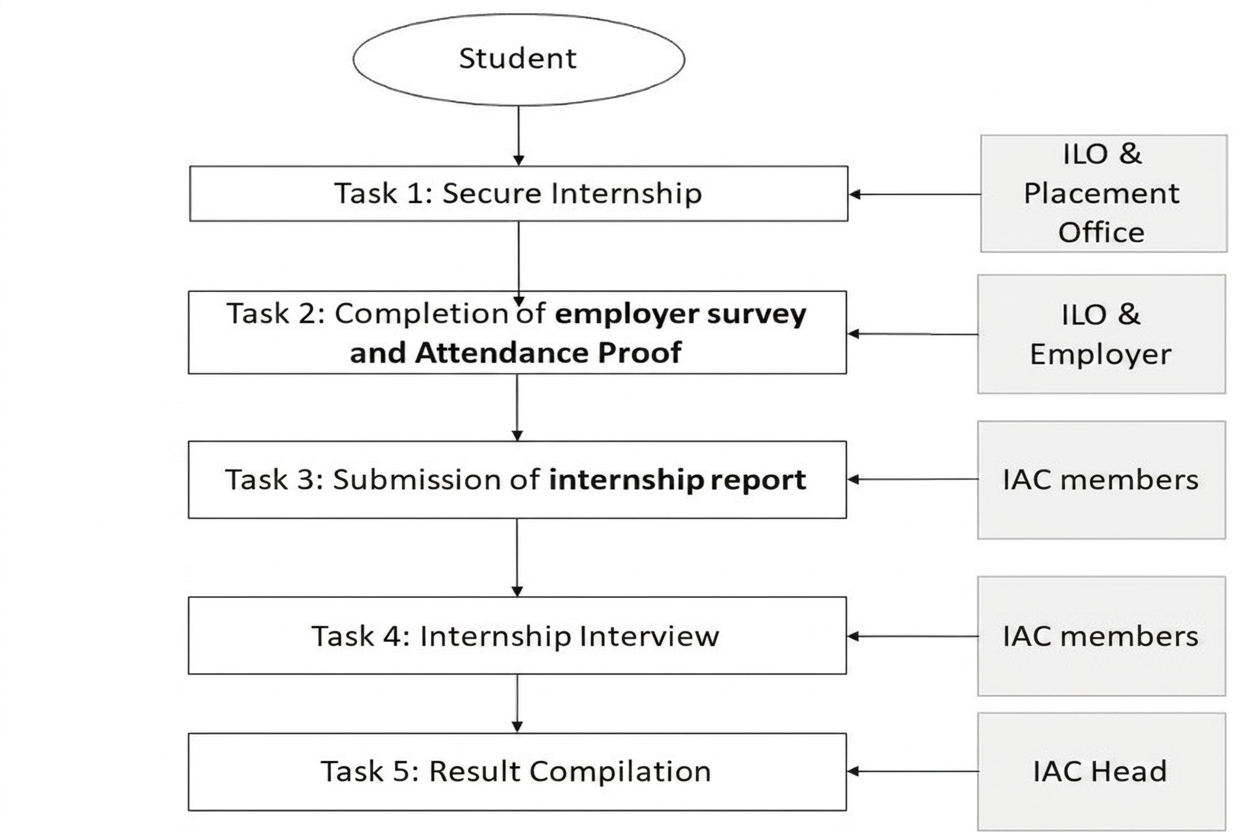
\includegraphics[width=1.0\textwidth]{images/criterion_3/media/img_internship_process.jpeg} % <-- Increased to 100%
\caption{Outline of internship program at SEECS}
\label{figure:Outline_of_internship_program_at_SEECS}
\end{figure}

\begin{table}[H]
\centering
\footnotesize % <-- Reduces font size
\renewcommand{\arraystretch}{0.85} % <-- Tightens vertical row spacing
\caption{Hierarchy of Internship Assessment Committee}
\label{tab:Hierarchy_of_Internship_Assessment_Committee}
\begin{tabular}{>{\raggedright\arraybackslash}p{0.30\textwidth}
                >{\raggedright\arraybackslash}p{0.52\textwidth}}
\toprule
\textbf{Position} & \textbf{Role} \\
\midrule
IAC Head & Overall oversight and custodian of evaluation records \\
ILO (Industry Liaison Officer) & First point of contact for students; IAC member \\
IAC Members & Evaluation and interview of internees \\
\bottomrule
\end{tabular}
\end{table}

The internship feedback forms were revised recently to obtain indirect assessment of PLOs from the employers of interns. The detailed analysis of PLO attainment based on internship feedback for the 2K21, 2K22, and 2K23 batches has already been presented in Section~\ref{sec:internshipfeedback}. The results presented in that section provide evidence of PLO attainment based on employer feedback. Table~\ref{tab:Summary_of_Students_from_Different_Batches_under_the_SEECS_Internship_Program} provides a summary of students who have successfully completed summer internships. BESE 2K23 is currently under evaluation but 24 have already successfully completed the entire process.

\begin{table}[H]
\centering
\footnotesize % <-- Reduces font size
\renewcommand{\arraystretch}{0.85} % <-- Tightens vertical row spacing
\caption{Batch-wise Summary of Students Completing Internship Program}
\label{tab:Summary_of_Students_from_Different_Batches_under_the_SEECS_Internship_Program}
\begin{tabular}{>{\raggedright\arraybackslash}p{0.30\textwidth}
                >{\centering\arraybackslash}p{0.25\textwidth}}
\toprule
\textbf{Batch} & \textbf{No.\ of Completed Internships} \\
\midrule
BESE 2K21 & 85 \\
BESE 2K22 & 81 \\
BESE 2K23 & 24 \\
\midrule
\textbf{Total} & \textbf{190} \\
\bottomrule
\end{tabular}
\end{table}

\hypertarget{sec:4.9othermethods}{%
\section{Additional Learning Methods}\label{sec:4.9othermethods}}

NUST SEECS provides students with various opportunities to participate in workshops, training programs, seminars, and short courses. Some of these activities are presented in Table~\ref{tab:Workshops_Training_Programs_Seminars_and_Short_Courses}. These activities enhance academic, technical, and research competencies while providing exposure to emerging technologies and industry trends. They also promote interaction with academic and industry experts contributing to continuous improvement of the academic programs.  Additionally, regular language courses are also offered to facilitate students aiming to pursue higher education or work abroad. These courses include \emph{Arabic, French, and German}. 

\begin{table}[H]
\centering
\footnotesize % <-- Reduces font size
\renewcommand{\arraystretch}{0.85} % <-- Tightens vertical row spacing
\caption{Workshops Training Programs Seminars and Short Courses}
\label{tab:Workshops_Training_Programs_Seminars_and_Short_Courses}
\begin{tabular}{c p{2cm} p{5.5cm} p{3cm}}
\toprule
\textbf{\begin{tabular}[c]{@{}c@{}}Sr.\\ No.\end{tabular}} & \textbf{Type} & \textbf{Title} & \textbf{Date} \\ 
\midrule

1 & Workshop & Building Capacity with AI for Sustainable Ventures & November 19, 2025 \\ \addlinespace

2 & Workshop & Reinforcement Learning Unleashed: Hands-On Skill Building for Smarter AI & August 18-22, 2025 \\ \addlinespace

3 & Workshop & Resilient Futures: GeoAI for Farms \& SLUMs---Robotics and Remote Sensing for Pakistan's Sustainable Well-Being & October 9, 2025 \\ \addlinespace

4 & Training Program & Programming for AI Systems & July 8, 2024 - September 8, 2024 \\ \addlinespace

5 & Seminar & Unlocking Business Value with AI and Data Analytics & May 2, 2024 \\ \addlinespace

6 & Workshop & FinTech Frontier: Harnessing the Power of LLMs & February 21-23, 2024 \\ \addlinespace

7 & Short Course & A four day short course on Sensors and AI & June 5-8, 2023 \\ 

\bottomrule
\end{tabular}
\end{table}

\begin{comment}
\hypertarget{sec:4.10assessment}{%
\section{Assessment of Learning Outcomes}\label{sec:4.10assessment}}

{\color{red}The learning outcomes at both course level and program level are measured in a direct and indirect manner, described in detail in Criterion~2 (Sections~3.6.1 to~3.6.4).}

\hypertarget{sec:gaattainment}{%
\subsection{Attainment of Graduate Attributes (GAs)}\label{sec:gaattainment}}

The BESE curriculum ensures coverage of all Knowledge, Skills, and Attitude (KSA) domains across the eleven graduate attributes (PLOs). Graduate attribute attainment is measured at graduation level through direct assessment (coursework and FYDP rubrics) and indirect assessment (exit surveys and internship feedback), as described in Criterion~2.
\end{comment}


%\begin{figure}[H]
%\centering
%\includegraphics[width=\textwidth]{images/criterion_3/media/image16.png}
%\missingcriterionthreefigure{image16.png}
%\end{figure}


%-----------------------------------------------------------------------
\hypertarget{sec:4.11fydp}{%
\section{Final Year Design Projects}\label{sec:4.11fydp}}

The BESE program includes a Final Year Design Project (FYDP) which is a design/research-oriented activity spanning the last two semesters and serving as the pinnacle activity for inculcating desired graduate attributes through solutions to complex engineering problems, guided by the FYDP policy (Annexure~\ref{app:criteria-3_FYP_Guidelines}). The FYDP is evaluated through oral presentation, documentation, and poster design across proposal defense, mid-defense, open house, and final defense with the complete evaluation process outlined in Annexure~\ref{app:criteria-3_FYP_Guidelines} and OBE-based assessment described in Section~\ref{sec:FYDP}

\begin{comment}
\begin{figure}[H]
\centering
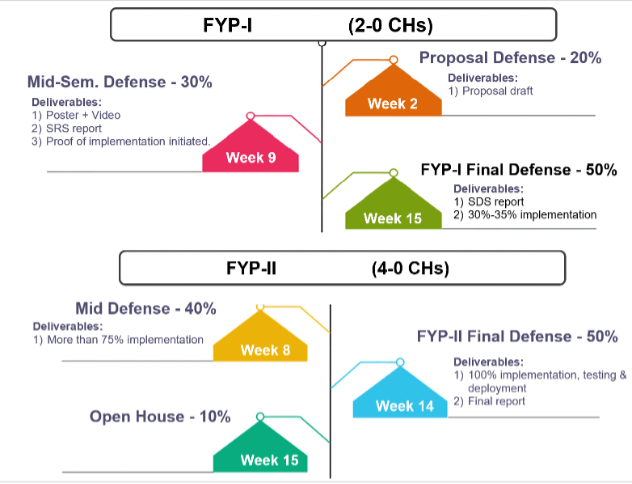
\includegraphics[width=0.8\textwidth]{images/criterion_3/media/img_fydp_process.png}
\caption{Roadmap of Final Year Design Project}
\label{figure:Roadmap_of_Final_Year_Design_Project}
\end{figure}
\end{comment}

The FYDP assessments shown in Figure~\ref{figure:fydp1} provide direct evaluation of PLOs. The PLO mapping for each FYDP semester (7 \& 8) of Batch 2k23 is listed in Table~\ref{tab:Mapping_of_FYDP_to_Direct_Assessment_of_PLOs-12} while the PLO mapping for the subsequent batches is shown in Table~\ref{tab:Mapping_of_FYDP_to_Direct_Assessment_of_PLOs-11}. Each activity is measured through rubrics which are shared with students at project initiation (Annexure~\ref{app:criteria-3_FYP_Guidelines}). Mid-defense, final report, and final presentation evaluations are conducted by a committee comprising of domain experts (relevant faculty members). The marks obtained in each activity stage are recorded in TMS and are used for final result compilation. Table~\ref{tab:distribution} shows percentage weightage of each activity in FYDP assessment. Best Industrial Project and Overall Best Project for Rector's Gold Medal are selected at the end of FYDP via a competitive process where shortlisted projects undergo a final round of presentation and evaluation by two separate committees. 

\begin{figure}[H]
\centering
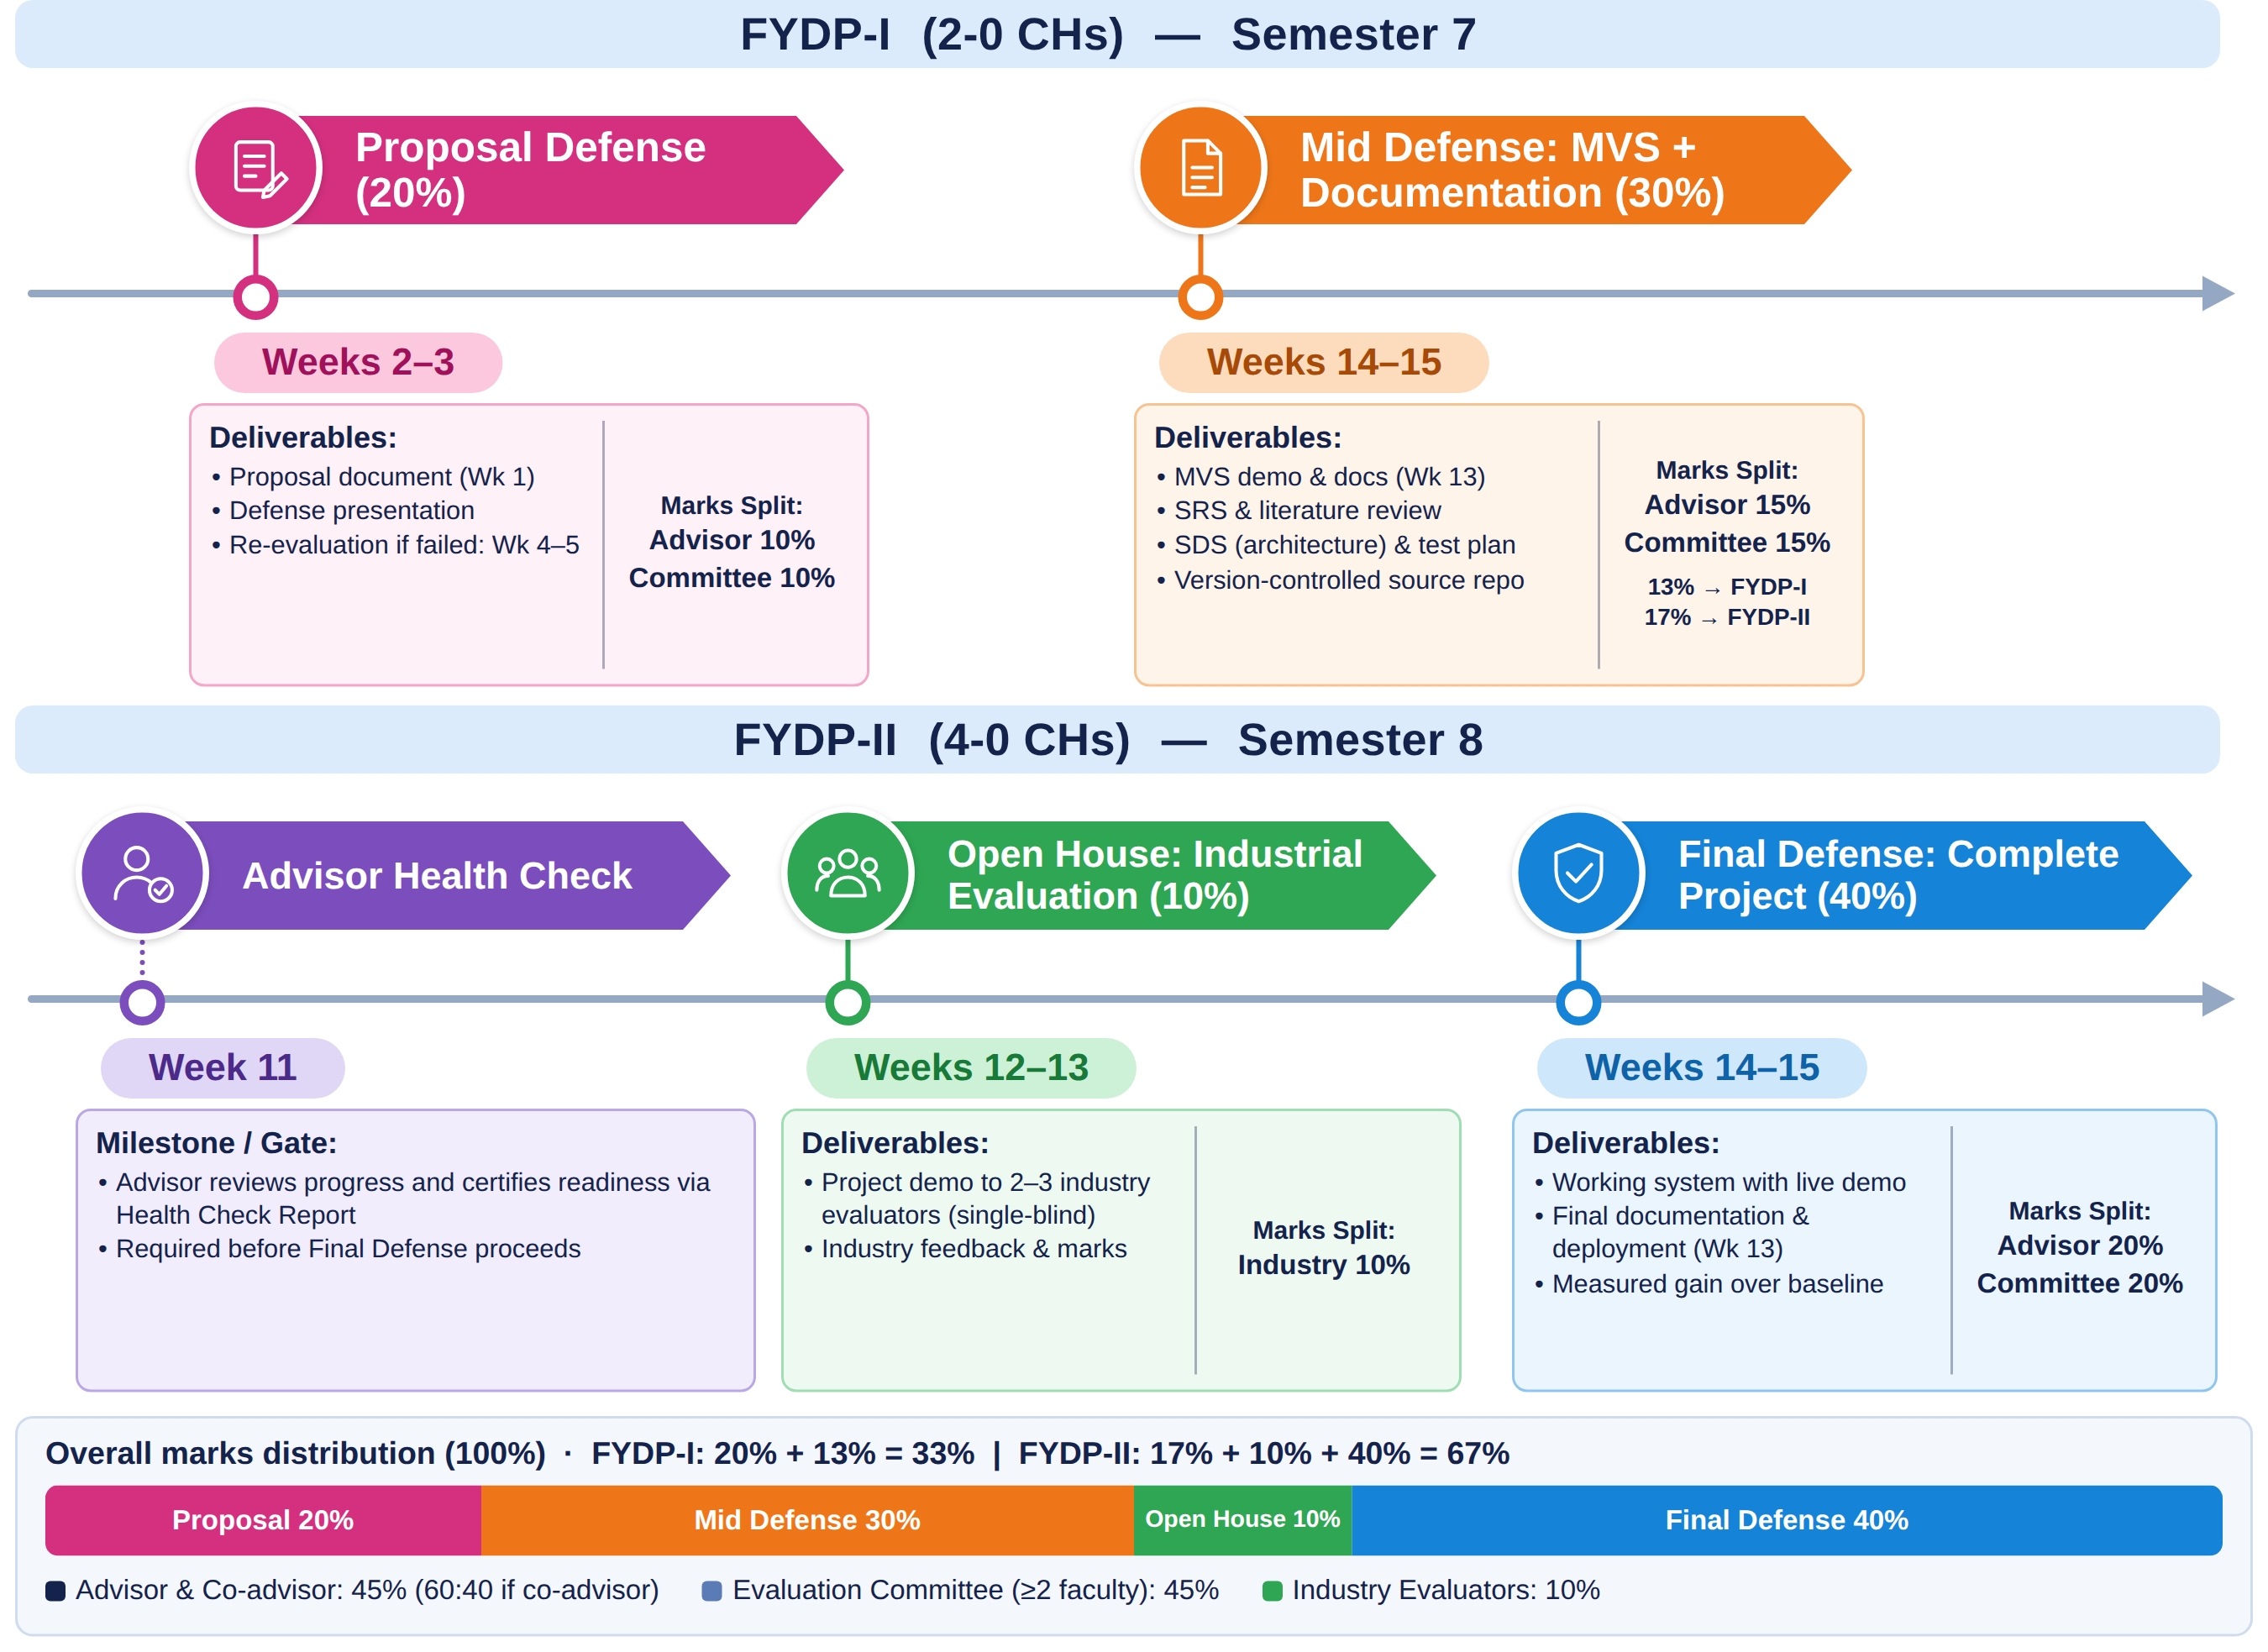
\includegraphics[width=0.9\textwidth]{images/criterion_2/media/FYDP-timeline.png}
\caption{Roadmap of Final Year Design Project (FYDP) Across 7\textsuperscript{th} \& 8\textsuperscript{th} Semesters.}
\label{figure:fydp1}
\end{figure}


\begin{comment}
\begin{landscape}
\begingroup\scriptsize\setlength{\tabcolsep}{3pt}
\begin{longtable}{>{\raggedright\arraybackslash}p{0.07\linewidth}
                  >{\raggedright\arraybackslash}p{0.18\linewidth}
                  >{\centering\arraybackslash}p{0.058\linewidth}
                  >{\centering\arraybackslash}p{0.058\linewidth}
                  >{\centering\arraybackslash}p{0.058\linewidth}
                  >{\centering\arraybackslash}p{0.058\linewidth}
                  >{\centering\arraybackslash}p{0.058\linewidth}
                  >{\centering\arraybackslash}p{0.058\linewidth}
                  >{\centering\arraybackslash}p{0.058\linewidth}
                  >{\centering\arraybackslash}p{0.058\linewidth}
                  >{\centering\arraybackslash}p{0.058\linewidth}
                  >{\centering\arraybackslash}p{0.058\linewidth}
                  >{\centering\arraybackslash}p{0.058\linewidth}}
\caption{Mapping of FYDP to Direct Assessment of PLOs} \\
\label{tab:Mapping_of_FYDP_to_Direct_Assessment_of_PLOs} \\
\toprule
\textbf{Course} & \textbf{Title} & \textbf{PLO 1} & \textbf{PLO 2} & \textbf{PLO 3} & \textbf{PLO 4} & \textbf{PLO 5} & \textbf{PLO 6} & \textbf{PLO 7} & \textbf{PLO 8} & \textbf{PLO 9} & \textbf{PLO 10} & \textbf{PLO 11} \\
& & \scriptsize Eng.Know. & \scriptsize Prob.Anal. & \scriptsize Design/Dev. & \scriptsize Invest. & \scriptsize Tool Usage & \scriptsize Eng.\&World & \scriptsize Ethics & \scriptsize Teamwork & \scriptsize Commun. & \scriptsize Proj.Mgmt. & \scriptsize Lifelong \\
\midrule
\endfirsthead
\multicolumn{13}{l}{\footnotesize\textit{Continued from previous page}} \\
\toprule
\textbf{Course} & \textbf{Title} & \textbf{1} & \textbf{2} & \textbf{3} & \textbf{4} & \textbf{5} & \textbf{6} & \textbf{7} & \textbf{8} & \textbf{9} & \textbf{10} & \textbf{11} \\
\midrule
\endhead
\bottomrule
\endlastfoot
SE-498 & Final Year Design Project -- I  & $\checkmark$ & $\checkmark$ & $\checkmark$ & $\checkmark$ & $\checkmark$ & $\checkmark$ & $\checkmark$ & $\checkmark$ & $\checkmark$ & $\checkmark$ & \\
SE-499 & Final Year Design Project -- II & $\checkmark$ & $\checkmark$ & $\checkmark$ & $\checkmark$ & $\checkmark$ & $\checkmark$ & $\checkmark$ & $\checkmark$ & $\checkmark$ & $\checkmark$ & $\checkmark$ \\
\end{longtable}
\endgroup
\end{landscape}
\end{comment}

\begin{table}[H]
\centering
\footnotesize % <-- Keeps size compact
\renewcommand{\arraystretch}{0.85} % <-- Tightens vertical padding
\caption{Mapping of FYDP to Direct Assessment of PLOs for 2K23 Batch (12-PLOs)}
\label{tab:Mapping_of_FYDP_to_Direct_Assessment_of_PLOs-12}
\begin{tabular}{c >{\raggedright\arraybackslash}p{0.42\textwidth} >{\centering\arraybackslash}p{0.18\textwidth} >{\centering\arraybackslash}p{0.18\textwidth}}
\toprule
\textbf{PLO \#} & \textbf{Program Learning Outcome} & \textbf{SE-498 (FYDP -- I)} & \textbf{SE-499 (FYDP -- II)} \\
\midrule
PLO 1  & Engineering Knowledge              & $\checkmark$ & $\checkmark$ \\
PLO 2  & Problem Analysis                   & $\checkmark$ & $\checkmark$ \\
PLO 3  & Design/Development of Solutions    & $\checkmark$ & $\checkmark$ \\
PLO 4  & Investigation                      & $\checkmark$ & $\checkmark$ \\
PLO 5  & Modern Tool Usage                  & $\checkmark$ & $\checkmark$ \\
PLO 6  & Engineer and Society      & $\checkmark$ & $\checkmark$ \\
PLO 7  & Environment and Sustainability        & $\checkmark$ & $\checkmark$ \\
PLO 8  & Ethics                             &  & $\checkmark$ \\
PLO 9  & Individual and Teamwork            & $\checkmark$ & $\checkmark$ \\
PLO 10  & Communication                      & $\checkmark$ & $\checkmark$ \\
PLO 11 & Project Management                 & $\checkmark$ & $\checkmark$ \\
PLO 12 & Lifelong Learning                  &              & $\checkmark$ \\
\bottomrule
\end{tabular}
\end{table}

\begin{table}[H]
\centering
\footnotesize % <-- Keeps size compact
\renewcommand{\arraystretch}{0.85} % <-- Tightens vertical padding
\caption{Mapping of FYDP to Direct Assessment of PLOs for 2K24 \& Onwards Batches (11-PLOs)}
\label{tab:Mapping_of_FYDP_to_Direct_Assessment_of_PLOs-11}
\begin{tabular}{c >{\raggedright\arraybackslash}p{0.42\textwidth} >{\centering\arraybackslash}p{0.18\textwidth} >{\centering\arraybackslash}p{0.18\textwidth}}
\toprule
\textbf{PLO \#} & \textbf{Program Learning Outcome} & \textbf{SE-498 (FYDP -- I)} & \textbf{SE-499 (FYDP -- II)} \\
\midrule
PLO 1  & Engineering Knowledge              & $\checkmark$ & $\checkmark$ \\
PLO 2  & Problem Analysis                   & $\checkmark$ & $\checkmark$ \\
PLO 3  & Design/Development of Solutions    & $\checkmark$ & $\checkmark$ \\
PLO 4  & Investigation                      & $\checkmark$ & $\checkmark$ \\
PLO 5  & Modern Tool Usage                  & $\checkmark$ & $\checkmark$ \\
PLO 6  & Engineer and Society       & $\checkmark$ & $\checkmark$ \\
PLO 7  & Ethics                             &  & $\checkmark$ \\
PLO 8  & Individual and Teamwork            & $\checkmark$ & $\checkmark$ \\
PLO 9  & Communication                      & $\checkmark$ & $\checkmark$ \\
PLO 10 & Project Management                 & $\checkmark$ & $\checkmark$ \\
PLO 11 & Lifelong Learning                  &              & $\checkmark$ \\
\bottomrule
\end{tabular}
\end{table}

\begin{table}[H]
\centering
\footnotesize % <-- Reduces font size
\renewcommand{\arraystretch}{0.85} % <-- Tightens vertical row spacing
\caption{Percentage of Weightage for Each FYDP Activity}
\label{tab:distribution}
\begin{tabular}{>{\raggedright\arraybackslash}p{0.30\textwidth}
                >{\centering\arraybackslash}p{0.25\textwidth}}
\toprule
\textbf{Activity} & \textbf{Percentage} \\
\midrule
Proposal Defense & 20\% \\
Mid Defense-I & 13\% \\
Mid Defense-II & 17\% \\
Open House & 10\% \\
Final Defense & 40\%\\
\midrule
\textbf{Total} & \textbf{100\%} \\
\bottomrule
\end{tabular}
\end{table}


\hypertarget{sec:fydpsdg}{%
\subsection{Mapping of FYDPs with UN SDGs}\label{sec:fydpsdg}}

All final year projects in the BESE program are mandatorily mapped to at least one UN Sustainable Development Goal (SDG), reflecting the program's commitment to socially responsible innovation and instilling in graduates a sense of global responsibility to address pressing challenges through software engineering. This ensures that projects demonstrate both technical proficiency and contribution to sustainability, equity, and social progress. The mapping of BESE-2K22 FYDPs to relevant UN SDGs is shown in Table~\ref{tab:Mapping_of_FYDPs_to_SDGs_for_BESE_Batch}. List of sample projects is presented in Annexure~\ref{app:criteria-3_List of FYDP BESE 2K22 Batch}.

\begin{comment}
\begin{table}[H]
\centering
\footnotesize % <-- Reduces font size
\renewcommand{\arraystretch}{0.85} % <-- Tightens vertical row spacing
\caption{Mapping of FYDPs to SDGs for BESE ?? Batch (BESE-??)}
\label{tab:Mapping_of_FYDPs_to_SDGs_for_BESE_Batch}
\begin{tabular}{>{\centering\arraybackslash}p{0.08\textwidth}
                >{\raggedright\arraybackslash}p{0.48\textwidth}
                >{\centering\arraybackslash}p{0.24\textwidth}}
\toprule
\textbf{S.No.} & \textbf{SDG} & \textbf{Number of Projects} \\
\midrule
1  & No Poverty & 0 \\
2  & Zero Hunger & 0 \\
3  & Good Health and Well-Being & 14 \\
4  & Quality Education & 7 \\
5  & Gender Equality & 2 \\
6  & Clean Water and Sanitation & 0 \\
7  & Affordable and Clean Energy & 0 \\
8  & Decent Work and Economic Growth & 7 \\
9  & Industry, Innovation and Infrastructure & 15 \\
10 & Reduced Inequalities & 2 \\
11 & Sustainable Cities and Communities & 7 \\
12 & Responsible Consumption and Production & 4 \\
13 & Climate Action & 5 \\
14 & Life Below Water & 0 \\
15 & Life on Land & 1 \\
16 & Peace, Justice and Strong Institutions & 3 \\
17 & Partnerships for Goals & 0 \\
\midrule
   & \textbf{Total Number of Projects} & \textbf{37} \\
\bottomrule
\end{tabular}
\end{table}
\end{comment}

\begin{table}[H]
\centering
\footnotesize
\renewcommand{\arraystretch}{0.85}
\caption{No. of FYDPs (BESE 2K22) Mapped to Relevant SDGs}
\label{tab:Mapping_of_FYDPs_to_SDGs_for_BESE_Batch}

\begin{tabular}{>{\centering\arraybackslash}p{0.08\textwidth}
                >{\raggedright\arraybackslash}p{0.48\textwidth}
                >{\centering\arraybackslash}p{0.24\textwidth}}
\toprule
\textbf{S.No.} & \textbf{SDG} & \textbf{Number of Projects} \\
\midrule

1  & No Poverty & 4 \\
2  & Zero Hunger & 3 \\
3  & Good Health and Well-Being & 11 \\
4  & Quality Education & 15 \\
5  & Gender Equality & 1 \\
6  & Clean Water and Sanitation & 1 \\
7  & Affordable and Clean Energy & 0 \\
8  & Decent Work and Economic Growth & 9 \\
9  & Industry, Innovation and Infrastructure & 17 \\
10 & Reduced Inequalities & 1 \\
11 & Sustainable Cities and Communities & 4 \\
12 & Responsible Consumption and Production & 6 \\
13 & Climate Action & 1 \\
14 & Life Below Water & 0 \\
15 & Life on Land & 0 \\
16 & Peace, Justice and Strong Institutions & 2 \\
17 & Partnerships for Goals & 0 \\

\bottomrule
\end{tabular}
\end{table}

\begin{comment}
{\footnotesize
\renewcommand{\arraystretch}{0.85}
\begin{longtable}{>{\centering\arraybackslash}p{0.08\textwidth}
                  >{\raggedright\arraybackslash}p{0.68\textwidth}
                  >{\centering\arraybackslash}p{0.10\textwidth}}
\caption{FYDP Projects -- BESE 2K22 Batch} \\
\toprule
\textbf{Sr.\#} & \textbf{Project Title} & \textbf{Dept.} \\
\midrule
\endfirsthead
\multicolumn{3}{l}{\footnotesize\textit{Continued from previous page}} \\
\toprule
\textbf{Sr.\#} & \textbf{Project Title} & \textbf{Dept.} \\
\midrule
\endhead
\midrule \multicolumn{3}{r}{\footnotesize\textit{Continued on next page}} \\
\endfoot
\bottomrule
\endlastfoot
1  & AI Based Security Orchestration, Automation, and Response System & SE \\
2  & OBE Assess: AI-Powered Outcome-Based Education Assessment System & SE \\
3  & CyberShield: Cybersecurity Awareness \& Incident Reporting Portal & SE \\
4  & Non-Technical Cofounder Super Agent (E-commerce) & SE \\
5  & HRXpert: Automating Talent Acquisition with Artificial Intelligence & SE \\
6  & EEGWriter: Multimodal Deep Learning Framework for Automated EEG Diagnostic Report Generation & SE \\
7  & AI-Driven UAV System for Disaster Response and Real-Time Rescue Operations & SE \\
8  & From Drones to Decisions: LLM-Based Crop Health Insights from RGB and Multispectral Data & SE \\
9  & Explainable AI for EEG Signal Classification (NeuroXplain) & SE \\
10 & EmergeOS: Autonomy-as-a-Service & SE \\
11 & Smart AgriAssist: AI-Powered Crop Disease Detection and Market Advisory System for Small Farmers in Pakistan & SE \\
12 & Disrupting Deepfake Generation Through Adversarial Attacks & SE \\
13 & Troubleshooting Copilot & SE \\
14 & Artificial Intelligence-Based End Point Detection and Response System & SE \\
15 & AI-Powered Profitability Estimation for Short-Term Rental Properties & SE \\
16 & Sedata.AI & SE \\
17 & Gaze-Guided Explainable AI for EEG-Based Brain Disorder Classification & SE \\
18 & SmartSketch: AI-Powered Facial Image Generator from Natural Language Descriptions & SE \\
19 & A Hybrid AI Framework for Dynamic Behavioral Adaptation & SE \\
20 & An Expert-Guided Multimodal AI Ecosystem for Diagnostic Intelligence & SE \\
21 & Smart Parental Control \& Monitoring System for Child Devices & SE \\
22 & Callisto AI: Conversational Intelligent CI/CD Automation Tool & SE \\
23 & AI-Assisted Forensic Analysis System for Decision Support & SE \\
24 & Cloud Optimization: Cost and Security for Enterprise Success & SE \\
25 & LiDAR-Based Plant Phenotyping for Precision Agriculture & SE \\
26 & Adaptive Web Interaction: Leveraging Reinforcement Learning for Comprehensive Action Support & SE \\
27 & FleaderAI: An AI-Driven End-to-End Lead Relationship Automation via Memory-Centric Conversational Agents & SE \\
28 & Emotion Detection from Micro-Expressions & SE \\
29 & Design and Development of a Decentralized B2B2C Platform for Skilled Labour Connectivity & SE \\
30 & InnBotics & SE \\
31 & HunarmandAI: Culturally-Aware Intelligent Tutoring for Low-Literacy Urdu Speakers & SE \\
32 & AI-Tutor for University Entry Test Preparation & SE \\
33 & Federated Data Lakes and Intelligent Healthcare Management for Pakistan & SE \\
34 & TaxSimplify: Automated Budgeting \& Tax Return Filing System & SE \\
\end{longtable}
}
\end{comment}

\subsection{Mapping of FYDPs with CEP Attributes}
\label{sec:fydpcep}
The Final Year Design Projects (FYDPs) are structured to provide students with opportunities to apply engineering knowledge and professional skills to complex, real-world software engineering problems. Table~\ref{tab:fydp_cep_mapping} presents the mapping of FYDP requirements and activities with the relevant CEP attributes.

\begin{table}[H]
\centering
\scriptsize % <-- Reduced font size from \footnotesize to \scriptsize
\renewcommand{\arraystretch}{0.70} % <-- Tightened vertical padding further
\caption{Mapping of FYDPs with CEP Attributes}
\label{tab:fydp_cep_mapping}
\begin{tabular}{>{\raggedright\arraybackslash}p{0.18\textwidth}
                >{\raggedright\arraybackslash}p{0.20\textwidth}
                >{\raggedright\arraybackslash}p{0.22\textwidth}
                >{\raggedright\arraybackslash}p{0.24\textwidth}}
\toprule
\textbf{Engineering Design Requirement} & 
\textbf{Evidence in FYDP Guidelines (Annex X)} & 
\textbf{Relevant Washington Accord WP(s)} & 
\textbf{Remarks} \\
\midrule

Problem Identification & 
Problem Definition chapter in Final Report Template & 
WP1 -- Depth of knowledge required, WP2 -- Conflicting requirements & 
Students identify, analyze, and justify a real-world engineering problem with multiple stakeholder needs and constraints. \\ \addlinespace[2pt]

Requirements Engineering & 
Software Requirements Specification (SRS) Template & 
WP2 -- Conflicting requirements, WP3 -- Depth of analysis required & 
Functional and non-functional requirements are elicited, analyzed, prioritized, and documented before implementation. \\ \addlinespace[2pt]

System Design & 
System Architecture and Detailed Design chapters & 
WP4 -- Familiarity of issues, WP5 -- Extent of applicable codes, WP6 -- Stakeholder involvement & 
Students design system architectures and components while considering standards, constraints, and stakeholder expectations. \\ \addlinespace[2pt]

Engineering Analysis & 
Methodology and Literature Review chapters & 
WP1 -- Depth of knowledge required, WP3 -- Depth of analysis required & 
Selection of algorithms, methodologies, tools, and technologies is justified through critical analysis and literature review. \\ \addlinespace[2pt]

System Implementation & 
Implementation \& Testing chapter & 
WP3 -- Depth of analysis required, WP7 -- Interdependence & 
The complete engineering solution is developed by integrating multiple software components and technologies. \\ \addlinespace[2pt]

System Validation & 
Results \& Discussion chapter & 
WP2 -- Conflicting requirements, WP7 -- Interdependence & 
The solution is verified and validated against the original requirements using appropriate testing and evaluation techniques. \\ \addlinespace[2pt]

Engineering Documentation & 
Standard report templates & 
WP5 -- Extent of applicable codes, WP6 -- Stakeholder involvement & 
The entire engineering design process is documented according to departmental templates, standards, and professional practices. \\

\bottomrule
\end{tabular}
\end{table}

%-----------------------------------------------------------------------
\hypertarget{sec:4.13grades}{%
\section{Grade Distribution}\label{sec:4.13grades}}

The Software Engineering Department at NUST-SEECS follow a relative grading system that uses A, B+, B, C+, C, D+, D, and F grades. The grade-wise distribution of results for all active BESE batches for the Spring~2026 End-Semester Examination is presented in Annexure~\ref{app:criteria-3_System of instruction and examination}. Details of the system are discussed in Section~\ref{sec:performance-evaluation}.
\begin{comment}
\clearpage
\begin{landscape}
\begingroup\scriptsize\setlength{\tabcolsep}{3pt}
\begin{longtable}{>{\raggedright\arraybackslash}p{0.08\linewidth}
                  >{\raggedright\arraybackslash}p{0.28\linewidth}
                  >{\centering\arraybackslash}p{0.047\linewidth}
                  >{\centering\arraybackslash}p{0.047\linewidth}
                  >{\centering\arraybackslash}p{0.047\linewidth}
                  >{\centering\arraybackslash}p{0.047\linewidth}
                  >{\centering\arraybackslash}p{0.047\linewidth}
                  >{\centering\arraybackslash}p{0.047\linewidth}
                  >{\centering\arraybackslash}p{0.047\linewidth}
                  >{\centering\arraybackslash}p{0.047\linewidth}
                  >{\centering\arraybackslash}p{0.047\linewidth}
                  >{\centering\arraybackslash}p{0.06\linewidth}}
\caption{Grade Distribution -- Intake Batch UG SE-2K22, ESE Spring 2026} \\
\toprule
\textbf{Course Code} & \textbf{Course Name} & \textbf{Total} & \textbf{A} & \textbf{B+} & \textbf{B} & \textbf{C+} & \textbf{C} & \textbf{D+} & \textbf{D} & \textbf{F} & \textbf{Remarks} \\
\midrule
\endfirsthead
\multicolumn{12}{l}{\footnotesize\textit{Continued from previous page}} \\
\toprule
\textbf{Course Code} & \textbf{Course Name} & \textbf{Total} & \textbf{A} & \textbf{B+} & \textbf{B} & \textbf{C+} & \textbf{C} & \textbf{D+} & \textbf{D} & \textbf{F} & \textbf{Rem.} \\
\midrule
\endhead
\bottomrule
\endlastfoot
CSL-402 & Community Service Learning A & 43 & 0 & 0 & 0 & 0 & 0 & 0 & 0 & 0 & Q \\
CSL-402 & Community Service Learning B & 43 & 0 & 0 & 0 & 0 & 0 & 0 & 0 & 0 & Q \\
CS-481  & Computer Forensics (A)       & 54 & 5 & 14 & 16 & 11 & 4 & 4 & 0 & 0 & \\
CS-416  & Large Language Models (Gp-01) & 47 & 8 & 10 & 13 & 7 & 5 & 2 & 2 & 0 & \\
CS-416  & Large Language Models (Gp-02) & 20 & 2 & 2 & 2 & 6 & 5 & 2 & 1 & 0 & \\
CS-415  & Mobile Application Development & 52 & 6 & 10 & 17 & 10 & 6 & 3 & 0 & 0 & \\
SE-499  & Final Year Design Project -- II & 85 & 69 & 16 & 0 & 0 & 0 & 0 & 0 & 0 & \\
\end{longtable}

\begin{longtable}{>{\raggedright\arraybackslash}p{0.08\linewidth}
                  >{\raggedright\arraybackslash}p{0.28\linewidth}
                  >{\centering\arraybackslash}p{0.045\linewidth}
                  >{\centering\arraybackslash}p{0.045\linewidth}
                  >{\centering\arraybackslash}p{0.045\linewidth}
                  >{\centering\arraybackslash}p{0.045\linewidth}
                  >{\centering\arraybackslash}p{0.045\linewidth}
                  >{\centering\arraybackslash}p{0.045\linewidth}
                  >{\centering\arraybackslash}p{0.045\linewidth}
                  >{\centering\arraybackslash}p{0.045\linewidth}
                  >{\centering\arraybackslash}p{0.045\linewidth}
                  >{\centering\arraybackslash}p{0.045\linewidth}}
\caption{Grade Distribution -- Intake Batch UG SE-2K23, ESE Spring 2026} \\
\toprule
\textbf{Code} & \textbf{Course Name} & \textbf{Total} & \textbf{A} & \textbf{B+} & \textbf{B} & \textbf{C+} & \textbf{C} & \textbf{D+} & \textbf{D} & \textbf{F} & \textbf{XF} \\
\midrule
\endfirsthead
\multicolumn{12}{l}{\footnotesize\textit{Continued}} \\
\toprule
\textbf{Code} & \textbf{Course Name} & \textbf{Total} & \textbf{A} & \textbf{B+} & \textbf{B} & \textbf{C+} & \textbf{C} & \textbf{D+} & \textbf{D} & \textbf{F} & \textbf{XF} \\
\midrule
\endhead
\bottomrule
\endlastfoot
MGT-271 & Entrepreneurship A & 44 & 6 & 15 & 21 & 2 & 0 & 0 & 0 & 0 & \\
MGT-271 & Entrepreneurship B & 41 & 5 & 21 & 15 & 0 & 0 & 0 & 0 & 0 & \\
SE-320  & Formal Methods A   & 44 & 7 & 9  & 12 & 10 & 4 & 1 & 0 & 1 & \\
SE-320  & Formal Methods B   & 41 & 6 & 12 & 16 & 6  & 1 & 0 & 0 & 0 & \\
CS-261  & Human Computer Interaction A & 44 & 2 & 13 & 16 & 9 & 3 & 0 & 1 & 0 & \\
CS-261  & Human Computer Interaction B & 41 & 4 & 16 & 15 & 6 & 0 & 0 & 0 & 0 & \\
CS-471  & Machine Learning A & 47 & 5 & 8  & 11 & 11 & 6 & 2 & 2 & 2 & \\
CS-471  & Machine Learning B & 43 & 3 & 13 & 17 & 5  & 2 & 1 & 1 & 1 & \\
SE-430  & Software Project Management A & 44 & 5 & 13 & 12 & 10 & 2 & 2 & 0 & 0 & \\
SE-430  & Software Project Management B & 43 & 4 & 14 & 17 & 6  & 2 & 0 & 0 & 0 & \\
SE-321  & Software Quality Engineering A & 44 & 4 & 8  & 10 & 12 & 7 & 2 & 0 & 1 & \\
SE-321  & Software Quality Engineering B & 42 & 5 & 11 & 16 & 7  & 3 & 0 & 0 & 0 & \\
\end{longtable}

\begin{longtable}{>{\raggedright\arraybackslash}p{0.08\linewidth}
                  >{\raggedright\arraybackslash}p{0.28\linewidth}
                  >{\centering\arraybackslash}p{0.043\linewidth}
                  >{\centering\arraybackslash}p{0.043\linewidth}
                  >{\centering\arraybackslash}p{0.043\linewidth}
                  >{\centering\arraybackslash}p{0.043\linewidth}
                  >{\centering\arraybackslash}p{0.043\linewidth}
                  >{\centering\arraybackslash}p{0.043\linewidth}
                  >{\centering\arraybackslash}p{0.043\linewidth}
                  >{\centering\arraybackslash}p{0.043\linewidth}
                  >{\centering\arraybackslash}p{0.043\linewidth}
                  >{\centering\arraybackslash}p{0.043\linewidth}}
\caption{Grade Distribution -- Intake Batch UG SE-2K24, ESE Spring 2026} \\
\toprule
\textbf{Code} & \textbf{Course Name} & \textbf{Total} & \textbf{A} & \textbf{B+} & \textbf{B} & \textbf{C+} & \textbf{C} & \textbf{D+} & \textbf{D} & \textbf{F} & \textbf{XF} \\
\midrule
\endfirsthead
\multicolumn{12}{l}{\footnotesize\textit{Continued}} \\
\toprule
\textbf{Code} & \textbf{Course Name} & \textbf{Total} & \textbf{A} & \textbf{B+} & \textbf{B} & \textbf{C+} & \textbf{C} & \textbf{D+} & \textbf{D} & \textbf{F} & \textbf{XF} \\
\midrule
\endhead
\bottomrule
\endlastfoot
MATH-232 & Complex Variables and Transforms A & 45 & 7 & 10 & 12 & 4 & 3 & 3 & 3 & 2 & 1 \\
MATH-232 & Complex Variables and Transforms B & 42 & 6 & 7  & 11 & 4 & 5 & 3 & 2 & 2 & 2 \\
CS-251   & Design \& Analysis of Algorithms A & 45 & 5 & 10 & 13 & 5 & 9 & 2 & 1 & 0 & 0 \\
CS-251   & Design \& Analysis of Algorithms B & 40 & 4 & 6  & 10 & 8 & 6 & 4 & 0 & 0 & 1 \\
HU-101   & Islamic Studies A & 41 & 8 & 20 & 10 & 2 & 1 & 0 & 0 & 0 & 0 \\
HU-101   & Islamic Studies B & 40 & 4 & 18 & 14 & 4 & 0 & 0 & 0 & 0 & 0 \\
CS-330   & Operating Systems A & 46 & 7 & 15 & 11 & 9 & 1 & 2 & 0 & 0 & 1 \\
CS-330   & Operating Systems B & 40 & 6 & 13 & 9  & 7 & 3 & 1 & 1 & 0 & 0 \\
MATH-361 & Probability and Statistics A & 44 & 5 & 15 & 16 & 5 & 2 & 0 & 0 & 1 & 0 \\
MATH-361 & Probability and Statistics B & 41 & 6 & 8  & 12 & 7 & 3 & 2 & 0 & 2 & 1 \\
SE-211   & Software Design and Architecture A & 44 & 7 & 18 & 15 & 3 & 1 & 0 & 0 & 0 & 0 \\
SE-211   & Software Design and Architecture B & 38 & 3 & 10 & 19 & 4 & 1 & 1 & 0 & 0 & 0 \\
\end{longtable}

\begin{longtable}{>{\raggedright\arraybackslash}p{0.08\linewidth}
                  >{\raggedright\arraybackslash}p{0.30\linewidth}
                  >{\centering\arraybackslash}p{0.045\linewidth}
                  >{\centering\arraybackslash}p{0.045\linewidth}
                  >{\centering\arraybackslash}p{0.045\linewidth}
                  >{\centering\arraybackslash}p{0.045\linewidth}
                  >{\centering\arraybackslash}p{0.045\linewidth}
                  >{\centering\arraybackslash}p{0.045\linewidth}
                  >{\centering\arraybackslash}p{0.045\linewidth}
                  >{\centering\arraybackslash}p{0.045\linewidth}
                  >{\centering\arraybackslash}p{0.045\linewidth}}
\caption{Grade Distribution -- Intake Batch UG SE-2K25, ESE Spring 2026} \\
\toprule
\textbf{Code} & \textbf{Course Name} & \textbf{Total} & \textbf{A} & \textbf{B+} & \textbf{B} & \textbf{C+} & \textbf{C} & \textbf{D+} & \textbf{D} & \textbf{F} \\
\midrule
\endfirsthead
\multicolumn{11}{l}{\footnotesize\textit{Continued}} \\
\toprule
\textbf{Code} & \textbf{Course Name} & \textbf{Total} & \textbf{A} & \textbf{B+} & \textbf{B} & \textbf{C+} & \textbf{C} & \textbf{D+} & \textbf{D} & \textbf{F} \\
\midrule
\endhead
\bottomrule
\endlastfoot
EE-122   & Computer Architecture \& Logic Design A & 43 & 8 & 16 & 10 & 6 & 3 & 0 & 0 & 0 \\
EE-122   & Computer Architecture \& Logic Design B & 45 & 6 & 7  & 11 & 9 & 9 & 3 & 0 & 0 \\
MATH-161 & Discrete Mathematics A & 42 & 7 & 12 & 10 & 3 & 7 & 1 & 1 & 1 \\
MATH-161 & Discrete Mathematics B & 44 & 5 & 7  & 11 & 8 & 11 & 0 & 2 & 0 \\
HU-114   & Functional English A & 43 & 5 & 14 & 16 & 7 & 1 & 0 & 0 & 0 \\
HU-114   & Functional English B & 44 & 7 & 14 & 20 & 2 & 1 & 0 & 0 & 0 \\
MATH-121 & Linear Algebra and ODEs A & 45 & 9 & 7  & 14 & 3 & 2 & 5 & 2 & 2 \\
MATH-121 & Linear Algebra and ODEs B & 45 & 2 & 11 & 12 & 6 & 6 & 2 & 5 & 3 \\
CS-212   & Object Oriented Programming A & 44 & 7 & 7  & 16 & 9 & 2 & 1 & 2 & 0 \\
CS-212   & Object Oriented Programming B & 45 & 6 & 7  & 11 & 9 & 9 & 3 & 0 & 0 \\
HU-132   & Understanding of Quran-II A & 42 & 15 & 19 & 7 & 0 & 1 & 0 & 0 & 0 \\
HU-132   & Understanding of Quran-II B & 41 & 9  & 13 & 11 & 8 & 0 & 0 & 0 & 0 \\
\end{longtable}
\endgroup
\end{landscape}
\end{comment}
%=======================================================================






\clearpage

% ============================================================
% CHAPTER 5 — Criterion 4: Students
% Images: images/criterion_4/media/
% ============================================================
\graphicspath{{images/criterion_4/media/}}
% Criterion 4: Students
% Updated from the authoritative DOCX dated 02-08-2026.
% Required packages in the main document:
%   graphicx, float, booktabs, array, multirow, hyperref
% Qalam evidence images are included conditionally when criterion4_assets is available.

\chapter{Criterion 4: Students}
\label{criterion4}

The success of the BESE program at NUST-SEECS is evaluated through the quality of admitted students, their academic progress, and the effectiveness of student support and quality assurance processes. The institute provides academic guidance, monitors progress towards program goals, and regularly reviews its procedures to maintain high standards. NUST-SEECS also promotes ethical values, interpersonal skills, and student well-being through sports, clubs, societies, professional chapters, and other co- and extracurricular activities. Admission is managed centrally by the NUST Admissions Directorate. Applicants must meet PEC eligibility requirements and take a competitive entrance examination. Merit is determined by performance in the admission examination and previous academic record, along with the applicant's stated program preferences.

\section{Eligibility Criteria and Admission Requirements}
\label{sec:admission-criteria}

Admission to the BE Software Engineering (BESE) programme at NUST-SEECS is
governed by NUST's undergraduate admission policy
(NUST Undergraduate Prospectus 2025)\footnote{NUST Undergraduate Prospectus 2025,
\url{https://nust.edu.pk/wp-content/uploads/2020/03/MARCOMS-PROSPECTUS-2025-V.5.0-04032025_compressed.pdf}.
The prospectus for the respective admission year applies to each batch.}
and the minimum eligibility requirements prescribed by the Pakistan Engineering
Council (PEC). The admission process ensures that candidates meet the prescribed
academic qualifications, possess an eligible subject background, and satisfy the
university's merit-based selection criteria. The principal eligibility
requirements are summarized in Table~\ref{tab:admission-eligibility}.

\begin{table}[htbp]
\centering
\caption{Eligibility Criteria for Admission to BE Software Engineering}
\label{tab:admission-eligibility}
\small
\renewcommand{\arraystretch}{1.2}
\begin{tabular}{|p{0.25\textwidth}|p{0.67\textwidth}|}
\hline
\textbf{Requirement} & \textbf{Eligibility Criteria} \\ \hline
SSC / Matriculation & Minimum 60\% aggregate marks or equivalent. \\ \hline
HSSC / Intermediate & Minimum 60\% aggregate marks or equivalent, with an accepted subject combination. \\ \hline
Pre-Engineering & Mathematics, Physics, and Chemistry. \\ \hline
ICS / Computer Science & Mathematics, Physics and Computer Science; eligible for all Engineering programmes subject to clearing Chemistry as a remedial course in the first semester. \\ \hline
Pre-Medical & Eligible for Engineering programmes either by passing NUST’s additional Mathematics exam, or by completing NUST’s 8-week condensed Mathematics course prior to admission. \\ \hline
O/A Levels or foreign qualifications & Relevant IBCC equivalence certificates demonstrating compliance with the prescribed subject and minimum-mark requirements. \\ \hline
Admission test and merit & Participation in the applicable NUST Entry Test (NET) and fulfilment of the university's merit-based selection criteria. \\ \hline
\end{tabular}
\end{table}

Candidates must hold at least 60\% aggregate marks in SSC and HSSC (or equivalent). FSc candidates may apply on FSc Part-I marks, with admission confirmed on submission of the FSc certificate or Detailed Marks Certificate showing at least 60\% aggregate. Candidates with an HSSC Pre-Engineering background must have studied Mathematics, Physics, and Chemistry. Candidates with an ICS/Computer Science background must have studied Mathematics, Physics, and Computer Science and are required to clear Chemistry as a remedial subject in the first semester, in accordance with the applicable policy. Eligible candidates from the Pre-Medical group may apply subject to fulfilment of NUST's prescribed condensed Mathematics requirements. Candidates holding O/A Level or other foreign qualifications must provide the relevant equivalence certificates issued by the Inter Board Committee of Chairmen (IBCC), demonstrating compliance with the prescribed subject and minimum-mark requirements. Admission is merit-based and processed through the NUST Entry Test (NET) and the university's prescribed selection procedure. The process is managed centrally by the NUST Admissions Directorate, which applies the approved eligibility criteria and merit determination procedure, as summarized in Table~\ref{tab:admission-merit}.

\begin{table}[H]
\centering
\caption{Admission Category Percentage}
\label{tab:admission-merit}
\begin{tabular}{@{}lc@{}}
\toprule
\textbf{Category} & \textbf{Percentage} \\
\midrule
NUST Entry Test & 75\% \\
HSSC / A Level / Equivalent / DAE or HSSC Part-I & 15\% \\
Matriculation / O Level\textsuperscript{*} & 10\% \\
\bottomrule
\end{tabular}
\vspace{0.4em}
\begin{minipage}{0.92\textwidth}
\footnotesize
\textsuperscript{*}O/A Level final-year candidates are assigned 25\% to O Level equivalence as per the IBCC certificate.
\end{minipage}
\end{table}

Compliance with PEC's minimum admission requirements is supported by the published admission policy, verification of candidates' academic qualifications and subject combinations, NET results, merit lists, IBCC equivalence certificates, and records of remedial-course completion, where applicable. These measures promote transparent admissions and provide documentary evidence for assessing compliance with the applicable PEC requirements. 

\section{Annual Intake and Admission Response}
\label{sec:annual-intake}
The programme's annual intake is also considered in relation to its approved capacity and available academic resources. The annual student intake, admission response, and current enrollment for batches 2K23, 2K24, 2K25, and 2K26, are outlined in Table~\ref{tab:annual-intake}. %, which can also be found in \hyperref[annex:D1]{Annex D1}.

%\begin{table}[htbp]
%\centering
%\caption{Annual Intake and Admission Response}
%\label{tab:annual-intake}

%\normalsize
%\renewcommand{\arraystretch}{1.25}
%\setlength{\tabcolsep}{9pt}

%\begin{tabular}{lccc}
%\toprule

%\textbf{Intake Batch} &
%\makecell[c]{\textbf{Intake}\\
%             \textbf{(Allowed / Present)}} &
%\makecell[c]{\textbf{No. of Applicants}\\
%             \textbf{(/ Acceptance Rate)}} &
%\textbf{Sections} \\

%\midrule

%Fall 2023 & 90 / 88 & 14,525 / 0.6\% & 2 \\
%Fall 2024 & 90 / 88 & 12,084 / 0.7\% & 2 \\
%Fall 2025 & 90 / 87 & 13,522 / 0.6\% & 2 \\
%Fall 2026 & 90 / 88 & 15,124 / 0.6\% & 2 \\
%\midrule

%\textbf{Total} &
%\textbf{360 / 351} &
%-- &
%\textbf{8} \\

%\bottomrule
%\end{tabular}
%\end{table}

\begin{table}[htbp]
\centering
\caption{Annual Intake and Admission Response}
\label{tab:annual-intake}
\small
\begin{tabular}{c l c c c c c}
\toprule
\textbf{\makecell{Sr.\\No.}} &
\textbf{\makecell[l]{Intake\\Batch}} &
\textbf{\makecell{Total\\Applicants}} &
\textbf{\makecell{Total Admissions\\Offered$^{*}$}} &
\textbf{\makecell{Acceptance\\Rate (\%)}} &
\textbf{\makecell{Present\\Strength}} &
\textbf{\makecell{No. of\\Section(s)}} \\
\midrule
1 & Fall 2023 & 14525 & 90 & 0.61\% & 85  & 2 \\
2 & Fall 2024 & 12084 & 90 & 0.74\% & 88  & 2 \\
3 & Fall 2025 & 13522 & 90 & 0.66\% & 88  & 2 \\
4 & Fall 2026 & 15124 & 90 & 0.59\% & 88  & 2 \\
\midrule
 & \textbf{Total} & \textbf{55255} & \textbf{360} & -- & \textbf{349} & -- \\
\bottomrule
\end{tabular}

\vspace{2pt}
\begin{flushleft}
\footnotesize $^{*}$ Total admissions offered in all the merit lists.
\end{flushleft}
\end{table}

%\section{Policy \& Processes for Transfer/Migration }
%\label{sec:student-transfer}

%Transfers are considered only on justifiable grounds and with approval of the Rector on the recommendation of the Principal, in accordance with NUST, HEC, and PEC regulations. The existing NUST policy permits migration after completion of the first year and before the final year; requires an academic record comparable with NUST admission standards; and, for transfers from another institution, requires a No Objection Certificate and a good-character/disciplinary-status certificate. Internal migration is restricted to students admitted through the NUST Entry Test.

\phantomsection
\section{Policies and Processes for Credit Transfer and Exemption}
\label{app:criteria3-credit-transfer}

NUST regulates credit transfer through two policies: the \textit{Migration and Transfer Policy}\footnote{Policy Code 26-00-005-04, approved 22 December 2021} and the \textit{Policy on Change of UG Program/Disciplines} (Annexure~\ref{annex:D1}). Both are administered by the Registrar Directorate, with academic evaluation carried out by the concerned school or college.

\subsection{Eligibility of Courses}
Credit is granted only for courses that satisfy the following conditions:
\begin{itemize}
    \item The student has earned at least a \textbf{B grade} in the course.
    \item The course corresponds to a NUST course, or is equivalent to one in depth and intensity.
    \item The student completes at least \textbf{60\%} of the credit hours of the degree programme at NUST.
\end{itemize}
Transferred credits count toward degree requirements, but their grades are \textbf{not} included in the CGPA calculation. Detailed requirements regarding parent institute, timeline, \% of CH, and NOC are outlined in Annexure~\ref{annex:D1}.

\subsection{Process}
\begin{enumerate}
    \item \textbf{Application:} The student submits the prescribed form with the official transcript, detailed course outlines, an NOC from the parent institution and the processing fee.
    \item \textbf{Course evaluation:} The receiving school or college evaluates the transcript and course outlines. It then lists the \textit{accepted courses} (with credits and grades) and the \textit{deficient courses} that the student must still complete.
    \item \textbf{Recommendation:} The Principal/Dean/Commandant recommends or rejects the case, and the Registrar Directorate processes it.
    \item \textbf{Approval:} The Rector approves migration cases, and the competent authority approves internal change-of-program cases.
\end{enumerate}

\subsection{Credit Treatment by Case}
\begin{table}[htbp]
\centering
\small
\begin{tabular}{p{3.6cm} p{9cm}}
\toprule
\textbf{Case} & \textbf{Credit Treatment} \\
\midrule
Migration from another institution & Accepted courses are credited after evaluation. Deficient courses must be completed at NUST. \\
Transfer within NUST & Allowed once only. Credits are evaluated by the receiving institute. \\
Change of program (first year common) & Accepted credits and grades are fully transferable. Leftover courses are recorded as non-credit additional courses, and the institute prepares a plan to make up any single deficient course. \\
Change of program (first year not common) & The student chooses Option~I (start afresh with no credit transfer) or Option~II (transfer of all accepted credits, with previous study time counted in the duration). Leftover courses are recorded as non-credit additional courses. \\
\bottomrule
\end{tabular}
\end{table}

\subsection{Related Conditions}
Students who migrate, or who change programs with credit transfer, are not eligible for honours and awards, except the Rector's Gold Medal. A change of program is allowed only once and cannot be reversed.

\begin{sloppypar}
Before acceptance, the required process evaluates course content, credit hours, grades, and learning outcomes for work completed in a PEC-accredited program of an HEC-recognized institution. No more than 50\% of the degree credit hours may be transferred, and each accepted transfer must be recorded and intimated to PEC at the time of acceptance. The transfer and migration policy is attached as Annexure~\ref{annex:D1}.
\end{sloppypar}


\section{Academic Counselling and Student Advisory System (SAS)}
\label{sec:sas}

%Each student is assigned a faculty advisor at the start of the program. The advisor serves as the student's first point of contact for academic matters, personal guidance, and professional development throughout the degree. The Student Advisory System (SAS) policy and related forms are provided in Annexure~\ref{annex:D2}.

%Students are organized into advisory groups of approximately 10--20 students. Several faculty members serve as Student Advisors under the supervision of the Department's Student Advisory Coordinator. The advisors monitor academic progress, attendance, conduct, and general well-being, and refer matters requiring specialized intervention to the relevant office. Advisory meetings are held several times every semester. Students with weak academic performance are counselled individually and may be directed towards coaching, tutoring, or other support. Records of advisory meetings and follow-up actions are maintained; representative records are provided in \hyperref[annex:D4]{Annex D4}.

%The advisory record is retained in Qalam and is visible to the relevant academic and administrative personnel. This provides transparency, traceability, and support for academic quality assurance.

Each critical student is supported by a faculty Student Advisor (SA) who serves as the first point of contact for academic matters, personal guidance and professional development. Advising is mandatory for all first-year students and for critical students, meaning those whose cumulative or semester GPA is below the qualifying grade or who have more than one F/XF/W grade. It is voluntary for other students, and the Head of Institution may add any student to the system. The Student Advisory System (SAS) policy and related forms are provided in Annexure~\ref{annex:D2}. 

Several faculty members serve as Student Advisors under the supervision of the Department's Student Advisory Coordinator. Critical students are assigned to dedicated advisors, with a maximum of 10 students per advisor. Advisor allocation for critical students identified in Fall 2026 are shown in Figure~\ref{fig:critical}. 

\begin{figure}[H]
\centering
\fbox{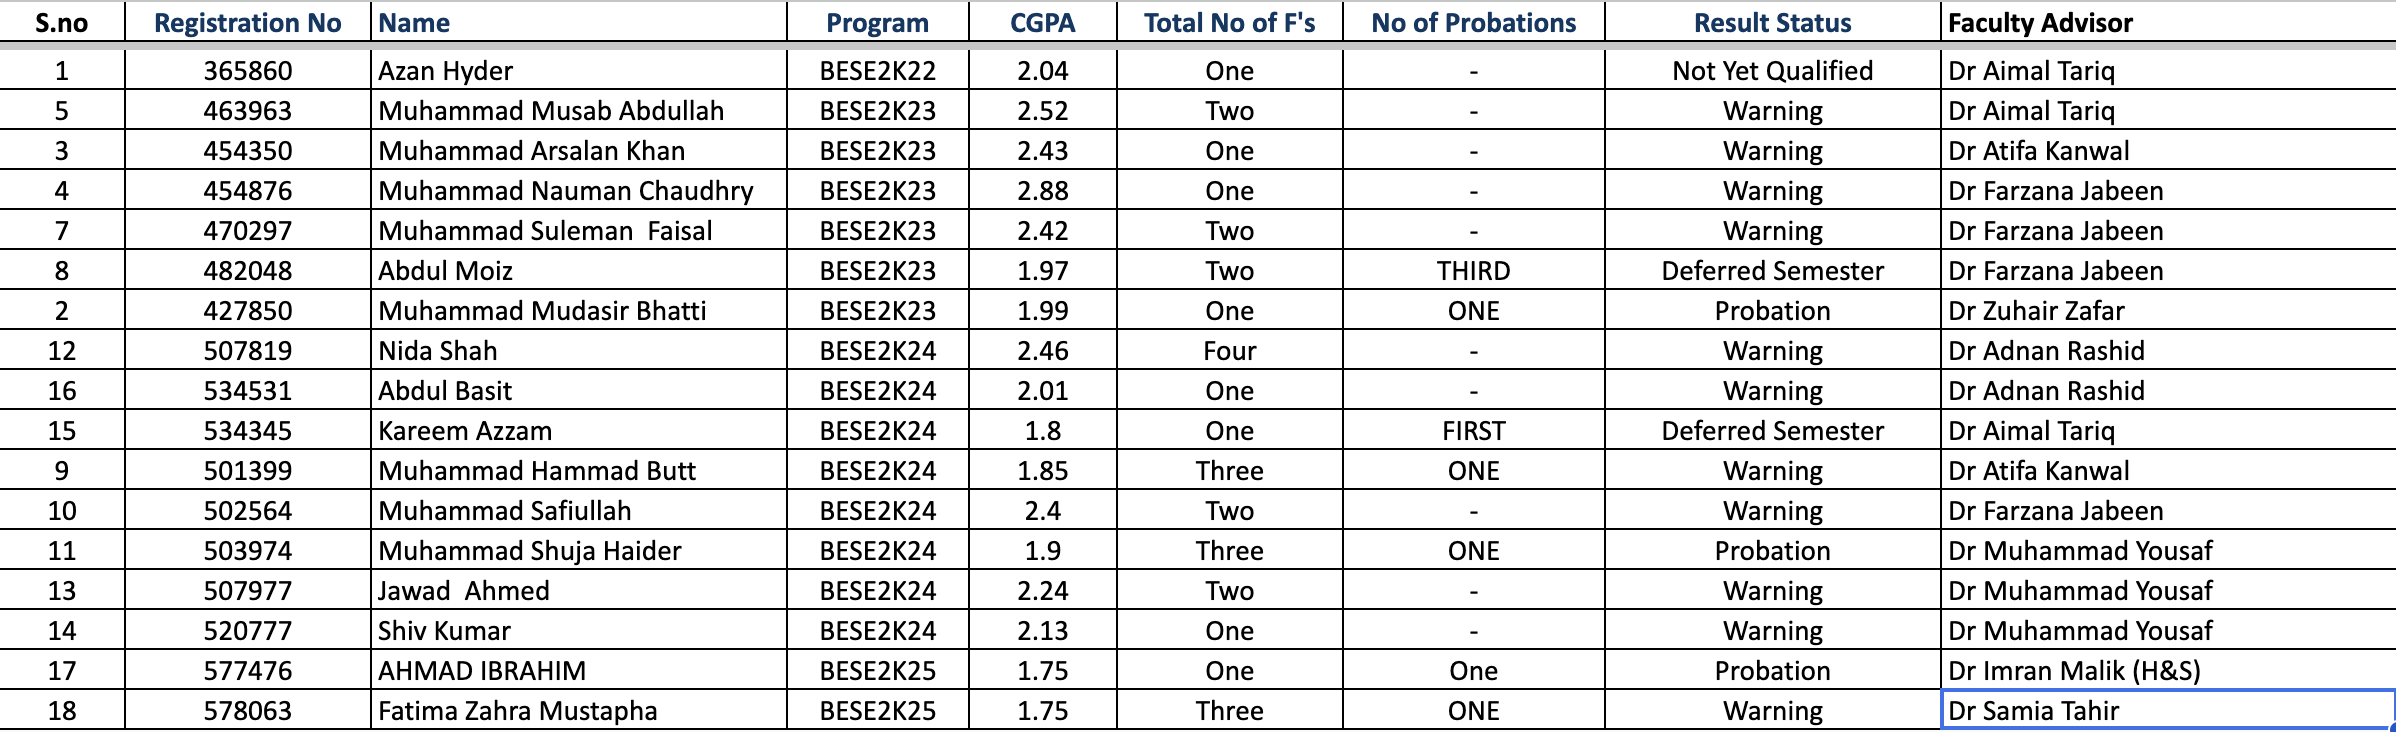
\includegraphics[width=1.0\textwidth]{images/criterion_4/critical.png}}
\caption{Advisor Allocation to Critical Students Identified in Fall 2026}
\label{fig:critical}
\end{figure}

The advisors monitor academic progress, attendance, conduct, and general well-being, and refer matters requiring specialized intervention to the relevant office. Parents are often contacted if required to keep them in the loop. Advisory meetings are held multiple times in each semester and are scheduled by the Academic Coordination Branch (ACB) (Figure~\ref{fig:schedule}). 

\begin{figure}[H]
\centering
\fbox{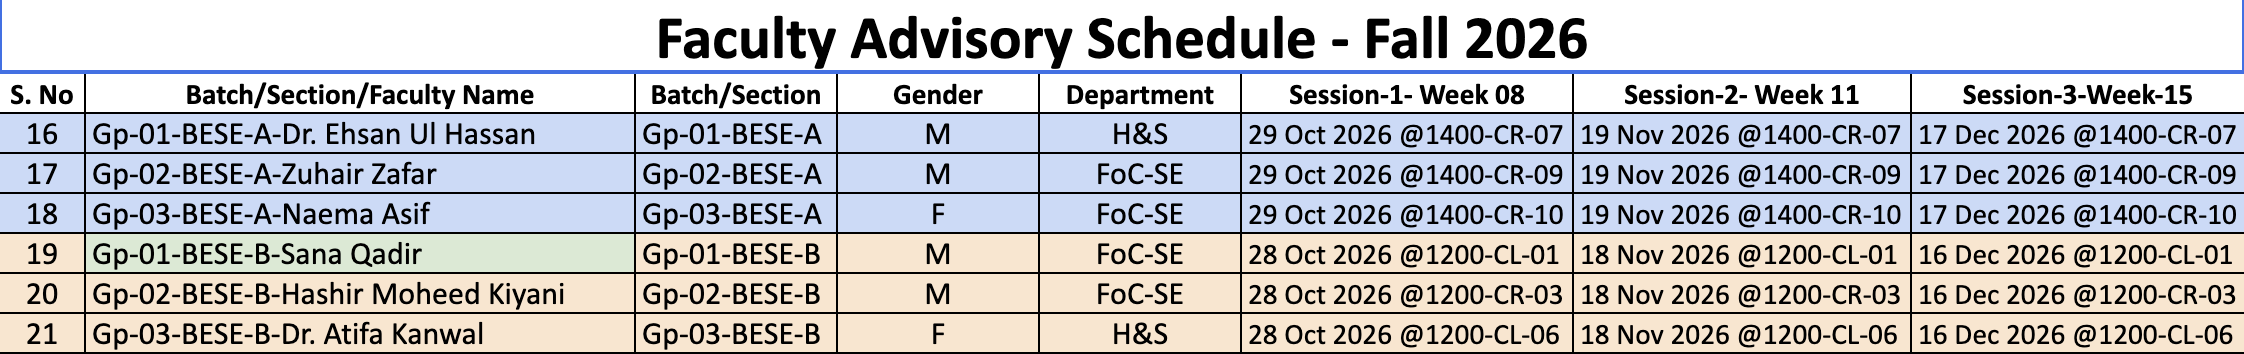
\includegraphics[width=1.0\textwidth]{images/criterion_4/schedule.png}}
\caption{Schedule for SAS Meetings in Fall 2026}
\label{fig:schedule}
\end{figure}

Students with weak academic performance are counselled individually and may be directed towards coaching, tutoring, or other support. Records of advisory meetings and follow-up actions are maintained (sample template for advisory record is presented in Annexure~\ref{annex:D3}). Reporting for critical students is automated in Qalam, which identifies them after results are announced, generates their academic progress sheets, supports advisor feedback reports and issues warning letters. 

\section{Career and Student Wellness Counselling}
\label{sec:career-wellness}

A formal orientation is conducted during the first week of each new batch to brief students on program requirements, academic regulations, support services, and professional expectations. The NUST Student Support Services Centre (S3C) serves as a one-window facilitation point. C3A provides professional counselling for academic, social, emotional, stress-related, and psychological concerns and conducts psychological assessments where appropriate. The Career Development Centre (CDC) supports career exploration, professional development, employer engagement, industry sessions, interviews, and recruitment drives. Further details are also discussed in subsequent chapters.


\section{Policies Dealing with Harassment \& Plagiarism}
\label{sec:plag}
\subsection{Academic Misconduct}
The NUST Code of Conduct (Undergraduate Student Handbook, Chapter~11) defines academic dishonesty as any act of fraud intended to influence a grade or academic evaluation. It covers cheating, fabrication, plagiarism, facilitating dishonesty and unauthorized collaboration. The use of unfair means, such as possessing unauthorized material or communicating with others during a test or examination, is also prohibited. Suspected cases are reported to the head of the institution through the Head of Department. The Institution Discipline Committee holds a hearing and gives the student a full opportunity to present his or her viewpoint before recommending a punishment. Penalties are proportional to the gravity of the case. Minor punishments include a written warning, probation, a fine of up to Rs~10,000, removal of privileges and the award of an F grade in the course. Major punishments include expulsion from class for up to one semester, a fine of up to Rs~50,000, cancellation of examination results, rustication, non-conferment of the degree and relegation or withdrawal. Minor punishments are awarded by the head of the institution, and major punishments for civilian students are awarded by the Rector on the recommendation of the NUST Discipline Committee. The student may appeal to the head of the institution or the Rector within fifteen days of the decision, and the parents of students who violate the Code are informed. Reference from UG Student Handbook is presented in Annexure~\ref{annex:D4} while complete handbook is available at SEECS Website\footnote{https://seecs.nust.edu.pk/wp-content/uploads/2024/09/28-Aug-2024-Undergraduate-Handbook.pdf}.
\subsection{Research-Related Plagiarism}
Research-related plagiarism and ethics cases are governed by the NUST Research Ethics and Plagiarism Policy\footnote{https://seecs.nust.edu.pk/wp-content/uploads/2020/06/Plagiarism-Policy-approved.pdf}, which complements the HEC Anti-Plagiarism Policy. The policy applies to all students, teachers, researchers and staff involved in research. Complaints are submitted to the Research Directorate with supporting evidence, and cases are heard by the NUST Standing Committee on Plagiarism and Research Ethics, chaired by the Pro-Rector (RIC). The committee works independently, members with a conflict of interest withdraw, the identities of those involved are kept confidential, and all parties are given a fair chance to present their case. Its decision is communicated to all stakeholders. All publications, theses and assignments are screened through Turnitin, and in line with HEC guidelines overall similarity must not exceed 19\% and similarity with any single source must not exceed 5\%.
\subsection{Zero-tolerance Policy on Harassment}
NUST follows a zero-tolerance policy on harassment\footnote{https://c3a.nust.edu.pk/wp-content/uploads/2020/11/NUST-Policy-on-Protection-Against-Harassment-6.pdf}, aligned with the Protection Against Harassment of Women at the Workplace (Amendment) Act 2022 and the HEC 2025 guidelines. The policy applies to students, faculty, staff and third parties, on campus, in NUST-recognized activities and online. Complaints may be informal (verbal or written, resolved by confidential mediation for lower-degree cases) or formal (written), and can be raised through focal persons, student advisors, supervisors, the HoD or Principal, any Inquiry Committee member or the anti-harassment helpline. Formal complaints go to a three-member Inquiry Committee that includes at least one woman. It informs the respondent within 3 working days, receives a reply within 7 working days, and submits its recommendations to the Rector within 30 working days. The Rector implements the decision within 7 working days. Proceedings are confidential, both parties are treated under the principles of natural justice, and complainant and respondent sign a non-contact undertaking. Reprisals are prohibited, and interim measures such as schedule changes or temporary suspension may be applied. Penalties follow the NUST statutes for students and employees, and malicious complaints are themselves punishable. Either party may appeal within 30 working days to a three-member Appellate Body or to the Ombudsman. NUST also runs awareness and sensitization training for focal persons and committee members.

\section{Semester Workload and Class Size}
\label{sec:class-size}
The program is divided into 8 semesters with course load each semester following the standards set by PEC and HEC. Table~\ref{tab:credit-hours} shows the breakdown of CHs for each semester of current BESE batches.

\begin{table}[H]
\centering
\caption{Credit hours breakdown for each semester for Batch 2k23, 2k24 and 2k25 \& onwards}
\label{tab:credit-hours}
\resizebox{\textwidth}{!}{%
\begin{tabular}{@{}crrrrrr@{}}
\toprule
\multirow{2}{*}{\textbf{Semester}} & \multicolumn{3}{c}{\textbf{Batch 2k23 and 2k24}} & \multicolumn{3}{c}{\textbf{Batch 2k25 \& onwards}} \\
\cmidrule(lr){2-4}\cmidrule(l){5-7}
& \textbf{CHs Teaching} & \textbf{CHs Labs} & \textbf{Total Credit Hours} & \textbf{CHs Teaching} & \textbf{CHs Labs} & \textbf{Total Credit Hours} \\
\midrule
1 & 16 & 2 & 18 & 14 & 4 & 18 \\
2 & 13 & 5 & 18 & 15 & 3 & 18 \\
3 & 15 & 3 & 18 & 15 & 3 & 18 \\
4 & 15 & 3 & 18 & 16 & 2 & 18 \\
5 & 14 & 4 & 18 & 14 & $3+X$ & $17+X$ \\
6 & 16 & $1+X$ & $17+X$ & 16 & $1+X$ & $17+X$ \\
7 & 11 & $2+X$ & $13+X$ & 12/13/14 & 5/4/3 & 17 \\
8 & 7 & 7 & 14 & 8/9/10 & 7/6/5 & 15 \\
\midrule
\multicolumn{3}{r}{\textbf{Grand Total}} & \textbf{$134+X$} & \multicolumn{2}{r}{\textbf{Grand Total}} & \textbf{$138+X$} \\
\bottomrule
\end{tabular}%
}
\end{table}
The class size for theory and practical sessions is the same. The class size and sample lab size of active batches of the BESE program is summarized in Table~\ref{tab:class-size} and Table~\ref{tab:lab-size} respectively.

\begin{table}[H]
\centering
\caption{Class Size of Current Batches}
\label{tab:class-size}
\begin{tabular}{@{}clrrrr@{}}
\toprule
\textbf{Sr. No.} & \textbf{Batch} & \textbf{Year of Intake} & \textbf{Size} & \textbf{No. of Sections} & \textbf{Average/Section} \\
\midrule
1 & BESE-14 & 2023 & 85 & 2 & 42.5 \\
2 & BESE-15 & 2024 & 88 & 2 & 44 \\
3 & BESE-16 & 2025 & 88 & 2 & 44 \\
4 & BESE-17 & 2026 & 88 & 2 & 44 \\
\bottomrule
\end{tabular}
\end{table}

\begin{table}[H]
\centering
\caption{Sample of Lab Size}
\label{tab:lab-size}
\begin{tabular}{@{}clcc@{}}
\toprule
\textbf{Sr. No.} &
\textbf{Lab} &
\textbf{Number of Workstations} &
\textbf{Workstations per Student} \\
\midrule
1 & Computing Lab 4 & 45 & 1 \\
2 & Computing Lab 5 & 45 & 1 \\
\bottomrule
\end{tabular}
\end{table}

\section{Completion of Courses and Student Feedback}
\label{sec:course-feedback}

Student feedback is collected twice during each semester, once before the MSE and again before the ESE. At the end of each feedback cycle, faculty members whose feedback scores fall below 70\% are requested to meet with the HoD to discuss student concerns and identify measures to improve the overall learning experience. At the end of each course, students also give their feedback on the course through the Students Course Review Report. The student feedback report about the faculty is attached as Annexure~\ref{annex:D5}.

\section{Student Co- \& Extra Curricular Activities}
\label{sec:competitions}
NUST-SEECS circulates opportunities and encourages participation in various student clubs and societies. While students can join any club and society across NUST\footnote{https://sa.nust.edu.pk/directory/}, there are a list of clubs and societies initiated by SEECS students and faculty sponsors. These are listed below:

\begin{itemize}
    \item{Hack Club}
    \item{Entrepreneurs Club}
    \item{IEEE Chapter}
    \item{ACM Chapter}
    \item{Google Developers Chapter}
    \item{Game Developement Club}
    \item{Fitness Club}
    \item{Excursion Club}
\end{itemize}

Aside from the clubs and societies, students are facilitated and mentored by the faculty and the administrative staff to participate in various high impact national and international events. Recent examples in the existing record include SEECS and SE student participation in following prominant events:
\begin{itemize}
    \item Efabless AI Generated Design Contest,
    \item IMechE UAS Design Challenge Pakistan,
    \item Huawei ICT Competition,
    \item SOFTEC, the Kibo Robot Programming Challenge, and
    \item Finding Innovative \& Creative Solutions for Society (FICS)
\end{itemize}
The list of prominent participantions in various international/national competitions and exhibitions with in the last three years is provided in Annexure~\ref{annex:D6} while details will be provided in Evidence folder.

\subsection{Annual Sports Gala}
\label{subsec:sports-gala}

NUST/SEECS provides indoor and outdoor sports opportunities and conducts an annual Sports Gala involving undergraduate and postgraduate students as well as faculty. Activities include cricket, football, basketball, volleyball, table tennis, badminton, tennis, squash, athletics and tug of war.

\subsection{International Exposure}
\label{subsec:financial-support}

The NUST International Office also circulates semester-exchange opportunities through SEECS focal persons. The list of universities hosting NUST students for semester exchange is attached as Annexure~\ref{annex:D11}. SEECS and SE students have been availing these opportunities frequently. Example of recent student exchanges is given in Table~\ref{tab:exchange}. Further details are provided in Evidence folder.

\begin{table}[H]
\centering
\caption{Recent SE Student Semester Exchanges Under UGRAD Program}
\label{tab:exchange}
\begin{tabular}{@{}clcc@{}}
\toprule
\textbf{Sr. No.} &
\textbf{Student Name} &
\textbf{Semester} &
\textbf{University} \\
\midrule
1 & Aryan Zia & Spring 2026 & Sungkyunkwan University, South Korea \\
2 & Eisha Tur Raazia & Spring 2026 & Sungkyunkwan University, South Korea \\
\bottomrule
\end{tabular}
\end{table}

\subsection{Community Service Learning}
\label{sec:community-service}

Community Service Learning course (CSL-402) was introduced in Spring 2013 as an optional course for undergraduate and postgraduate students and was later made compulsory for final-year undergraduate students. It aims to develop civic sense, social responsibility, community engagement, and an understanding of social issues. The course carries 0--1 credit hour and includes six workshops covering community needs assessment, project planning, teamwork, communication, social responsibility, and reflective learning. Students complete at least 30 hours of community service; some activities may be performed on campus, while the remaining work is completed through approved philanthropic or community organizations under the guidance of a faculty advisor. The Spring 2025 course outline is provided in Annexure~\ref{annex:D7}.

\section{Student Performance Evaluation}
\label{sec:performance-evaluation}

Students are evaluated through assignments, quizzes, term projects, laboratories, the Mid Semester Examination (MSE), and the End Semester Examination (ESE). A typical distribution of marks is given in Table~\ref{tab:evaluation-distribution}.

\begin{table}[H]
\footnotesize
\centering
\caption{Typical Student Performance Evaluation}
\label{tab:evaluation-distribution}
\resizebox{0.8\textwidth}{!}{%
\begin{tabular}{@{}lclc@{}}
\toprule
\multicolumn{2}{c}{\textbf{Lab-based Course (3+1)\textsuperscript{*}}} & \multicolumn{2}{c}{\textbf{Non-Lab-based Course (3+0)}} \\
\cmidrule(lr){1-2}\cmidrule(l){3-4}
\textbf{Assessment Type} & \textbf{Percentage} & \textbf{Assessment Type} & \textbf{Percentage} \\
\midrule
\multicolumn{2}{l}{\textbf{Lab Theory (75\%)}} & & \\
Quizzes & 10--15\% & Quizzes & 10--15\% \\
Assignments & 5--10\% & Assignments & 5--10\% \\
Mid Semester Exam & 25--35\% & Mid Semester Exam & 25--35\% \\
Semester Project & 0--20\% & Semester Project & 0--20\% \\
End Semester Exam & 40--50\% & End Semester Exam & 40--50\% \\
\addlinespace
\multicolumn{2}{l}{\textbf{Lab (25\%)}} & & \\
Lab Work & 50--70\% & & \\
Lab Project & 10--20\% & & \\
Lab Final & 20--30\% & & \\
\bottomrule
\end{tabular}%
}
\end{table}

Most of these assessments are mapped to course CLOs. At the end of the semester, a comprehensive report is generated for each student, which demonstrates an accurate assessment of students' progress with respect to fulfilment of course CLOs, in a direct manner. The relative grading system uses A, B+, B, C+, C, D+, D, and F grades. An I grade is awarded when a student is absent from the final examination; a retest requires approval from the FBS. An XF grade is awarded where attendance is below 75\%. A failed course may be repeated in the summer semester or when next offered. The course instructor submits results to the HoD for consideration by the DBS. The results are then presented to the FBS, chaired by the Principal SEECS and attended by representatives of the NUST Examination Branch, for approval.

\section{KPI of Students Performance in Relation to PLOs}
\label{sec:kpi-plo}

The suitability and affectivity of the teaching methodology and assessment methods are checked by reviewing the overall PLO results of a course. In case the PLOs are not achieved or have low direct and indirect assessment results, the LQEC recommends appropriate action. Details are discussed in subsequent chapters. For a cohort level issue, instructor is asked to review the teaching and assessment methodology and suggest an action for improvement. The PEOs, PLOs and CLOs of the program and their mapping are explained in detail in previous chapters.

\section{Financial Support}
\label{sec:fin}
Students can avail financial assistance via performance-merit awards, NUST need-based/Trust Fund assistance, Honhaar/HEC, and provincial scholarships, PEC need-cum-merit support, fee deferment, and Ihsan Trust interest-free loans. Sample list of students currently receiving financial support is attached as Annexure~\ref{annex:D10}.




\clearpage

% ============================================================
% CHAPTER 6 — Criterion 5: Faculty and Support Staff
% Images: images/criterion_5/media/
% ============================================================
\graphicspath{{images/criterion_5/media/}}
% Criterion 5 chapter converted from the approved Word source.
% Expected packages in the main document: array, booktabs, longtable,
% multirow, graphicx, hyperref, calc, enumitem, and float.
\providecommand{\real}[1]{#1}
%\usepackage{multirow}


\hypertarget{criterion-5-faculty-and-support-staff}{%
\chapter{Criterion 5: Faculty and Support Staff}\label{criterion-5-faculty-and-support-staff}}

The Department of Software Engineering at SEECS, NUST, maintains a complement of dedicated and shared faculty, supported by lab engineers, to facilitate effective student-faculty interaction and the delivery of the undergraduate program curriculum. Faculty members possess diverse academic qualifications, professional experience, and areas of specialization to support the core and interdisciplinary components of the Software Engineering curriculum. This criterion presents the department's faculty strength, professional ranks, academic qualifications, areas of expertise, teaching responsibilities, and student-faculty ratio, together with the supporting staff resources required for effective program delivery. The relevant faculty duties and workload arrangements are discussed in the subsequent sections, with reference to the applicable NUST statutes and policies (Annexure~\ref{annex:AG}).

\section{Faculty Strength and Competencies}
\label{faculty-strength-and-competencies}

The department currently has 18 full-time dedicated faculty members, comprising one Professor, two Associate Professors, 12 Assistant Professors, and three Lecturers (Table~\ref{tab:headcount1}). In addition, six shared faculty members contribute to teaching in their respective areas of expertise, while five Lab Engineers support practical instruction and laboratory activities. The faculty complement provides coverage across Software Engineering, Artificial Intelligence, Information Security, and Applied Computing, supporting the core components of the program. Shared and visiting faculty from other disciplines support the interdisciplinary components of the program. The faculty's academic qualifications, professional designations, institutional backgrounds, experience, departmental affiliations, and joining dates are documented in Annexure~\ref{annex:I}. Annexure~\ref{annex:K} provides the current and preceding semesters' teaching workloads, distinguishing theory and practical credit hours for undergraduate and postgraduate courses, where applicable. %The list of faculty members registered with the Pakistan Engineering Council (PEC) is provided in Annexure~\ref{annex:M}.

\begin{table}[htbp]
\centering
\small
\setlength{\tabcolsep}{4pt}
\caption{Faculty Headcount by Category}
\label{tab:headcount1}
\begin{tabular}{@{}p{0.34\columnwidth}ccccc@{}}
\toprule
\textbf{Category} & \textbf{Prof.} & \textbf{Assoc. Prof.} &
\textbf{Asst. Prof.} & \textbf{Lect./LE} & \textbf{Total} \\
\midrule
Full-time dedicated faculty & 1 & 2 & 12 & 3 & 18 \\
Shared faculty              & 1 & 1 & 4 & -- & 6 \\
Visiting Engg. faculty              & -- & 1 & -- & -- & 1 \\
Lab Engineers               & -- & -- & -- & 5 & 5 \\
\bottomrule
\end{tabular}
\end{table}

\subsection{Faculty Qualifications and Professional Ranks}
\label{pyramid-of-academic-structure}

The department maintains a mix of academic ranks and qualifications to support curriculum delivery, student supervision, and academic development. Currently, there are 18 FTDF (Engineering and non-engineering) members, comprising one Professor, two Associate Professors, 12 Assistant Professors, and three Lecturers. As reported in the faculty qualification records, 11 FTDF members, hold PhD degrees, while seven FTFD members hold MS qualifications. The institute provides opportunities for professional advancement based on applicable policies and eligibility criteria. Three of the seven MS FTDF members are concurrently pursuing PhD degrees (Table~\ref{tab:high}). One of the lab engineers is also pursuing PhD degree. 

\begin{longtable}{|>{\centering\arraybackslash}p{1cm}
|>{\raggedright\arraybackslash}p{2.8cm}
|>{\raggedright\arraybackslash}p{1.7cm}
|>{\raggedright\arraybackslash}p{2.5cm}
|>{\raggedright\arraybackslash}p{3cm}|}

\caption{SE Faculty Pursuing PhD}
\label{tab:high}\\
\hline
\textbf{Sr. No.} &
\textbf{Name} &
\textbf{Host Country} &
\textbf{University} &
\textbf{Subject} \\
\hline
\endfirsthead

\hline
\textbf{Sr. No.} &
\textbf{Name} &
\textbf{Host Country} &
\textbf{University} &
\textbf{Subject} \\
\hline
\endhead

1 & Hirra Anwar & Pakistan & SMME-NUST & Robotics and AI \\
\hline

2 & Mobeena Shahzad & Pakistan & EME-NUST & Robotics and AI \\
\hline

3 & Ayesha Kanwal & Pakistan & SMME-NUST & Robotics and AI \\
\hline

\end{longtable}

\subsection{Full-Time Dedicated Faculty}
\label{full-time-dedicated-faculty}

The 18 full-time dedicated faculty members constitute the department's primary teaching and academic resource. Their qualifications, experience, and areas of expertise support the delivery of the Software Engineering curriculum, student advising, project supervision, and related academic activities. Their teaching contributions and workload distribution across the current and preceding semesters are documented in Annexure~\ref{annex:K}.

\subsection{Shared Faculty}
\label{shared-faculty}

Six non-engineering shared faculty members supplement the dedicated faculty by teaching courses within their respective areas of specialization. These faculty members are associated with other departments or academic programs and enable the department to draw on expertise beyond its dedicated faculty complement. Their designations, qualifications, experience, and departmental affiliations are recorded in Annexure~\ref{annex:I}, while their teaching contributions are documented in Annexure~\ref{annex:K}.

\subsection{Visiting and Adjunct Faculty}
\label{visiting-faculty}

The department engages Temporary Visiting Faculty (TVF), where required, to address specialized teaching needs that cannot be fully met through the available permanent faculty. Such appointments are particularly relevant to elective courses requiring industry-specific knowledge and professional experience. In appropriate cases, NUST PhD scholars may also be engaged as TVFs. University policy further permits eligible permanent faculty members to undertake additional teaching assignments as visiting faculty alongside their regular responsibilities. These arrangements provide flexibility in addressing specialized curricular requirements while maintaining the department's core reliance on its dedicated and shared faculty. There are two adjunct faculty members in the department as well namely Dr. Elena Gaura from Coventry University, UK, and Dr. Ali Imran Shariq from the Norwegian University of Science and Technology. 

\subsection{Student--Faculty Ratio}
\label{student-teacher-ratio}

The department has maintained a healthy student--faculty ratio since the undergraduate program commenced in 2010 (Annexure~\ref{annex:J}). The current student enrolment is 349, supported by 18 full-time dedicated faculty members, six shared faculty members, and one TVF. Five Lab Engineers provide additional support for laboratory-based teaching and practical activities. As summarized in Table~\ref{tab:ratio}, the student--faculty ratio is 15.44:1 when calculated against current enrolment and the faculty headcount (22.6) used for this calculation. Against the reported allowed student intake, the ratio is 15.92:1. Both ratios are better than the PEC guideline of 20:1, demonstrating that the reported faculty strength is sufficient to support effective student--faculty interaction. These ratios are reported in accordance with the applicable PEC accreditation criteria.

\begin{table}[!h]
\centering
\small
\setlength{\tabcolsep}{4pt}
\caption{Student-Faculty Ratio}
\label{tab:ratio}
\begin{tabular}{@{}p{0.34\columnwidth}ccccc@{}}
\toprule
\textbf{Category} & \textbf{PhD} & \textbf{MS/MSc} &
\textbf{BE/BSc} & \textbf{Total} & \textbf{PEC Criteria} \\
\midrule
Full-time dedicated faculty & 9 & 6 & 0 & 15 &  \\
(Engineering)&&&&&\\
\hline
Full-time dedicated faculty & 2 & 1 & 0 & 1.6 & Capped at 20\% of \\
(Non-Engineering)&&&&&MFS (8 FTDF/Sect.)\\
\hline
Shared faculty              & 4 & 2 & 0 & & Counted half \\
(Non-Engineering)&&&&3.5&Capped at\\
Shared faculty              & 1 & 0 & 0 & & 25\% of FTDF \\
(Engineering)&&&&&\\
\hline
Lab Engineers               & 0 & 3 & 2 & 2.5 & Counted half \\
&&&&&Capped at 20\%\\
&&&&&FTDF\\
\hline
\textbf{Total Faculty Count}&\textbf{16}&\textbf{12}&\textbf{2}&\textbf{22.6}&\\
\midrule
\textbf{Allowed Intake}&\multicolumn{5}{c}{360} \\
\textbf{Current Student Strength}&\multicolumn{5}{c}{349} \\
\midrule
Student--faculty ratio & \multicolumn{5}{c}{15.44:1} \\
(As per current enrollment)& \multicolumn{5}{c} {}\\
Student--faculty ratio & \multicolumn{5}{c}{15.92:1} \\
(As per allowed enrollment)&\multicolumn{5}{c} {}\\
\bottomrule
\end{tabular}
\end{table}

Overall, the department's dedicated and shared faculty resources, supported by laboratory personnel and specialist visiting appointments where needed, provide a basis for effective curriculum delivery and student engagement. The documented faculty qualifications, professional ranks, expertise, and teaching workloads provide supporting evidence of the department's capacity to cover the program's curricular requirements.

%All members of the NUST fraternity assigned to teaching, research, and academic management activities comprise faculty. The faculty at SEECS includes the Principal, Associate Deans, Heads of Departments, Professors, Associate and Assistant Professors, and Lecturers. The faculty duties have been specified in NUST Statutes VI and are attached as Annexure~\ref{annex:AG}. 


%Faculty positions since the start of the undergraduate program in 2010 have been improving gradually. Relevant data since the last visit of the PEC Accreditation Committee, related to faculty summary, is given in Annex~\ref{annex:J}. Total enrolled students presently are 348. There are 14 full-time dedicated engineering faculty members. Full-time dedicated non-engineering faculty members are 3. Based on the criteria given in section 3.2.5.3 of the revised PEC accreditation manual, the student-teacher ratio comes to 17.53. Detailed calculations are given in Table 6.1 below.



\section{Training and Mentoring on Pedagogical Skills and OBE}
\label{sec:training}

SEECS has recently formalized a staged mechanism for training and mentoring faculty members in pedagogical skills and Outcome-Based Education (OBE) concepts. Formalized through the SEECS Faculty On-Boarding Guide (Version 1.0, published September 11, 2026\footnote{Faculty-On-Boarding-Guide-v1.0-1.pdf}), this framework operates at the Department and School level (provided in Evidence Folder). Newly inducted faculty members must also complete a NUST-level on-boarding training prior to and during their first semester of teaching conducted by NUST Center for Teaching and Learning (NCTL).

\subsection{Multi-Tier Mentoring and Training Mechanism}
Faculty training operates across a multi-tiered structure:
\begin {itemize}
\item \textbf{NUST Level:} Newly appointed faculty undergo a structured onboarding program covering    instructional delivery, class conduct, effective communication techniques, teaching methodologies, and lecture preparation. Operational training is conducted for the NUST LMS, Qalam CMS, and E-Office platforms. These mandatory sessions are organized by NCTL.

\item \textbf{(SEECS) Level:} At the school level, SEECS facilitates continuous training and guidance through:

\begin{itemize}
    \item \textbf{Knowledge Groups:} Knowledge Group Heads (KGHs) provide domain-specific oversight, vetting course outlines, mid-semester exams (MSE), end-semester exams (ESE), and retake papers for alignment with OBE standards.
    \item \textbf{Mentoring:} A senior faculty mentor is assigned to guide the inductee throughout their first semester in syllabus delivery, lab conduct, assessment vetting, and grading criteria.  
\end {itemize}
    
\end{itemize}

\subsection{OBE Concepts and Implementation Methodologies}

Faculty follow a systematic mechanism to gain a thorough operational understanding of Program Educational Objectives (PEOs), Program Learning Outcomes (PLOs), and Course Learning Outcomes (CLOs). 
\begin {itemize}[noitemsep, topsep=0pt]
\item \textbf{OBE Trainings:} OBE trainings are frequently held to enhance the understanding of faculty members regarding OBE framework followed at SEECS (Annexure~\ref{annex:T}). Each faculty member provides an overview of OBE framework to the students of their respective classes at the beginning of the semester. Students are also detailed during orientation session.
\item \textbf{Assessment Mapping:} Faculty builds a detailed assessment map linking each evaluation item (quizzes, assignments, exams, and practical labs) directly to approved CLOs and Bloom's difficulty levels mentioned in the approved course outline. 
\item \textbf{System Integration:} OBE data is configured in the Qalam Campus Management System (CMS) gradebook to aggregate mapped marks and generate real-time direct CLO–PLO attainment reports. 
\item \textbf{Continuous Quality Improvement (CQI):} Course folders maintained on the Learning Management System (LMS) include attainment reports and instructor CQI action plan to address any outcomes falling below target thresholds.
\end{itemize}

\subsection{Effectiveness of Training and Mentoring}
The efficacy of the training framework is measured through multi-faceted feedback loops:   
\begin{itemize}[noitemsep, topsep=0pt]
    \item \textbf{Student Course Evaluations:} Conducted digitally via Qalam at the end of each semester to track student satisfaction and instructional quality over successive terms.
    \item \textbf{Peer Teaching Audits:} Periodic peer reviews assess lecture clarity, responsiveness, classroom management, and alignment with approved outlines.
    \item \textbf{CLO/PLO Attainment Metrics:} Automated Qalam reports evaluate cohort performance per outcome, triggering mandatory CQI interventions where target thresholds are missed. 
\end{itemize}

\section{Faculty Development for Professional Growth}
Faculty's professional growth is supported through institutional faculty development, professional training, mentoring, research engagement, and opportunities for academic and professional advancement. Faculty development activities include pedagogical and Outcome-Based Education (OBE) training, technical and research-oriented workshops, participation in national and international professional development programmes, and guidance provided through departmental and institutional mechanisms. 

NUST supports the professional growth of its faculty through the Professional Development Centre (PDC), established in July 2007 under an initiative of the Higher Education Commission (HEC). Recently, it has been developed into Iqbal Executive Development Centre (IEDC) that offers professional training using experienced facilitators, practical exercises, and case-based learning to strengthen professional competencies and institutional practices. Faculty development activities provide opportunities to enhance pedagogical skills, OBE implementation, research capabilities, and academic leadership. The effectiveness of these activities can be assessed through their application in teaching and research, career progression, faculty feedback, and retention trends, enabling the identification of further development needs and appropriate improvement measures. Evidence of these will be provided separately. Table~\ref{tab:training} shows some recent professional development trainings in which SE faculty participated.

\begin{longtable}{|>{\centering\arraybackslash}p{1cm}
|>{\raggedright\arraybackslash}p{4cm}
|>{\centering\arraybackslash}p{2cm}
|>{\raggedright\arraybackslash}p{2.7cm}
|>{\raggedright\arraybackslash}p{3.5cm}|}
\caption{Training and development of SEECS faculty}
\label{tab:training}
\hline
\textbf{Sr. No} & 
\textbf{Training/Short Course} & 
\textbf{Date} & 
\textbf{Attendee(s)} & 
\textbf{Organized by} \\ 
\hline
\endhead

1 & 
AI in Agriculture & 
3/23/2026 & 
Dr. Momina Moetesum & 
Asian Productivity Organization \\ 
\hline

2 & 
Reinforcement Learning Unleashed: Hands-On Skill Building for Smarter AI & 
08/18/2025 to 08/22/2025 & 
Dr. Zuhair Zafar & 
Machine Vision and Intelligent Systems (MachVIS) Lab, SEECS, National University of Sciences and Technology, Islamabad. \\ 
\hline

3 & 
AI for Manufacturing Industry & 
4/23/2025 & 
Dr. Momina Moetesum & 
Continuing Professional Development Program, Department of Electrical Engineering, Lahore College for Women University, Lahore. \\ 
\hline

4 & 
IEEE Learning \& Research for Pakistan students \& researchers: an overview of IEEE Xplore Digital Library & 
4/15/2026 & 
Dr. Momina Moetesum & 
A\&J Def Tek Consultants \\ 
\hline

5 & 
National Workshop on AI Use-case Development & 
11/12/2025 & 
Dr. Momina Moetesum & 
IGNITE \\ 
\hline

6 & 
"Research Smarter: Using Web of Science for Academic Success" & 
5/21/2026 & 
Dr. Faisal Shafait & 
Higher Education Commission (HEC) Pakistan \\ 
\hline

7 & 
IEEE Authorship and Open Access Symposium: Tips and Best Practices to Get Published from IEEE Editors & 
6/12/2026 & 
Dr. Ayesha Maqbool & 
IEEE \\ 
\hline

\end{longtable}

\hypertarget{faculty-workload}{%
\section{Faculty Workload Distribution}\label{faculty-workload}}
Faculty workload and general duties are covered in detail in Annexure~\ref{annex:AG}. All Faculty members, besides teaching, are also involved in other activities which primarily include:

\begin{itemize}[noitemsep, topsep=0pt]
\item Performing administrative duties 
\item Performing the duties of LQEC
\item UG FYDP Supervision 
\item MS \& PhD Thesis Supervision
\item Staff appointments
\item Program coordination
\item Invigilation 
\item Funded projects
\item Research publications
\end{itemize}

In most cases, regular teaching load is reduced to facilitate these activities. For instance, a waiver of 1 credit hour is awarded on supervision of a PhD scholar. Similarly, administrative tasks like heading a department is equivalent to 3 credit hours. Nonetheless, maximum non-teaching credit is equivalent to 6 credit hours. To streamline the equivalence formula for equating teaching load with administrative duties, NUST Academic policy is relied upon using which a faculty member's research and administrative duties are elucidated by assigning them credit hours. The total load of a faculty member is the sum of Teaching, Research and Administrative duties. 

\hypertarget{faculty-retention-and-career-planning}{%
\section{Faculty Retention and Career Planning}\label{faculty-retention-and-career-planning}}

NUST provides remuneration and benefits in accordance with the applicable
institutional statutes, service regulations, and employment terms. The NUST
Gazette and Statutes are available through the University's official
website.\footnote{NUST, \textit{NUST Gazette and Statutes}, available at:
\url{https://nust.edu.pk/downloads/nust-gazette-and-statutes/}.}
Faculty policies are summarised in the NUST Faculty Handbook\footnote{NUST,
\textit{Faculty Handbook}, Version 1.3, Chapters 3, 5, 6 and 8. Detailed rules
are contained in the NUST Human Resource Handbook.} and administered by the
Human Resource Directorate. The applicable pay arrangements depend on the
faculty member's employment category:

\begin{enumerate}
    \renewcommand{\labelenumi}{(\alph{enumi})}
    \item \textbf{NUST Faculty:} Salaries and benefits are determined in
    accordance with the applicable NUST Statutes and institutional
    regulations. Faculty may be appointed on the Tenure Track System (TTS),
    which NUST has adopted in parallel with the HEC framework since 2012.

    \item \textbf{Ministry of Defence Officers:} Remuneration is administered
    in accordance with the applicable Government of Pakistan pay scales and
    regulations.

    \item \textbf{Pakistan Army Officers:} Pay is administered according to
    the applicable military pay scales through the Controller Military
    Accounts.
\end{enumerate}

In addition to remuneration, NUST provides the following facilities and
benefits to support faculty welfare, professional development, and retention.

\begin{enumerate}
    \item \textbf{Career Progression and Performance Appraisal.}
    Faculty performance is reviewed annually through the Annual Appraisal
    Report (AAR), which combines self-assessment, student feedback collected
    twice per semester, class audit, and evaluation by the Head of Department
    and Dean. Research performance (publications, sponsored funding,
    commercialisation, and student supervision) is a weighted input to
    subsequent promotion decisions.

    \item \textbf{Leave.}
    Faculty are entitled to 20 days of casual leave and 48 days of earned
    leave per year. Leave for study or academic purposes is approved by the
    Pro-Rector (Academics).

    \item \textbf{On-Campus Accommodation and Security.}
    Residential accommodation is available to faculty members on a
    first-come, first-served basis in the Iqra and Isra apartments and villas
    of various sizes, as well as faculty messes for single occupants. The
    campus is protected by CCTV surveillance and guards at all entries and
    exits.

    \item \textbf{Medical Facilities and Health Insurance.}
    NUST operates an in-house Medical Center providing consultation,
    emergency treatment, ambulance service, and a pharmacy. In addition,
    contractual civilian faculty members are covered, together with their
    eligible dependents (spouse and children), under the NUST Group Health
    Insurance Scheme.\footnote{NUST, \textit{NUST Group Health Insurance
    Scheme for Contractual Faculty and Support Staff Officers (Civilian
    only): General Guidelines/Instructions}, Human Resource Directorate.}
    Enrolment and records are managed by the Human Resource Directorate, the
    NUST Medical Centre acts as the liaison office with the insurance company
    for card issuance, activation and reimbursement claims, and the Finance
    Directorate processes premium payments. Dependent eligibility lapses on
    the death of the dependent, on separation (spouse), on marriage (son or
    daughter), or when a son exceeds 23 years of age. Coverage is suspended
    during leave exceeding four months and resumes on return to duty. Where
    the insurance limit is exhausted, further medical expenditure may be
    claimed through the Medical Reserve Pool, subject to rationalisation at
    the rates prescribed by Armed Forces Hospitals. Medical benefits for
    faculty in other employment categories are provided in accordance with
    the applicable institutional policy and eligibility
    conditions.\footnote{NUST, \textit{Medical Policy 2015 (Revised)},
    available at:
    \url{https://nshs.nust.edu.pk/wp-content/uploads/2023/08/Medical-Policy.pdf}.}

    \item \textbf{Research and Publication Incentives.}
    NUST sponsors article publication charges for peer-reviewed journals as per policy\footnote{NUST Research Directorate, \textit{Publication Charges for
    Peer-Reviewed Journals Sponsored by Research Dte}, Working Paper
    No.~39, 61st ACM, 2021; and policy letters No.~0986/41/Research/NUST
    dated 16 February 2024 and 15 November 2024.} Only journals indexed in
    the Science Citation Index Expanded, Social Sciences Citation Index, or
    Arts and Humanities Citation Index of Web of Science and ranked in
    Quartile~1 or Quartile~2 of the Journal Citation Reports are eligible.
    Emerging Sources Citation Index journals are excluded. NUST may sponsor
    up to US\$1,800 for Quartile~1 articles and up to US\$1,200 for
    Quartile~2 articles, shared among the NUST authors by author order
    (sole author 100\%; two authors 60\%/40\%; three authors
    50\%/35\%/15\%; four authors 45\%/30\%/15\%/10\%). The quartile is taken
    from the JCR edition of the year of publication. Applications are
    submitted at least four weeks before the invoice due date and within
    three months of acceptance, with a Turnitin report and an undertaking
    against plagiarism, endorsed by the Principal of the institution. For
    Quartile~2 articles one case per faculty member is permitted per fiscal
    year. Invoices must be issued in the name of the NUST authors, with split
    invoices where foreign co-authors are involved. Exceptional cases may be
    considered for full charges. Faculty who claim publication charges are
    not eligible for a publication financial award. In addition, NUST
    sponsors registration fees and travel for peer-reviewed international
    conferences, subject to eligibility and availability of funds, and funds
    professional society memberships and journal subscriptions. Annual Best
    Teacher and Best Researcher awards carry prizes of Rs~75,000 at school
    level and Rs~150,000 at university level. Seed funding for research is
    available from the NUST R\&D Fund, and faculty are supported in obtaining
    external grants through the Research, Innovation and Commercialization
    Directorate.

    \item \textbf{Provident Fund.}
    Provident fund benefits are subject to the applicable institutional
    policies, employment terms, and eligibility requirements, which are
    maintained by the NUST Human Resource Directorate.

    \item \textbf{Service Gratuity.}
    NUST provides service gratuity in accordance with the applicable policy
    and eligibility requirements. The qualifying service period varies
    according to the employment category.\footnote{NUST, \textit{NUST
    Gratuity Policy}, Policy Code 08-00-001-04, available at:
    \url{https://nshs.nust.edu.pk/wp-content/uploads/2023/08/Gratuity.pdf}.}

    \item \textbf{Faculty Development.}
    The NUST Faculty Development Program, launched in 2002--03, sponsors
    faculty for PhD and MS-leading-to-PhD studies at reputed foreign
    universities. The 2025 prospectus reports that 430 scholars have been
    sent abroad, of whom 316 have rejoined. PhD-qualified faculty may be
    sponsored for 9--12 months of post-doctoral research abroad, subject to
    availability of funds. A structured continuing professional development
    programme of seven modules covers orientation, instructional
    development, research writing, administrative and personal development,
    and short courses.

    \item \textbf{Reasonable Faculty Workload and Support for Higher
    Studies.}
    The average teaching load of a faculty member does not exceed 12 credit hours and may be reduced for administrative responsibilities, approved research, laboratory and course
    development, and supervision of theses and projects. SEECS endeavours to
    distribute teaching and other academic responsibilities reasonably, in
    accordance with applicable PEC guidelines and institutional requirements.
    Where feasible, workload allocation also takes account of the academic
    development needs of early-career faculty members pursuing higher
    studies, while maintaining the continuity and quality of teaching,
    research, and departmental activities. Compliance with the applicable
    workload requirements is supported by departmental workload records.

    \item \textbf{Welfare and Family Support.}
    Counselling services through the Center for Counseling and Career
    Advisory (C3A) are free of charge for NUST faculty and their immediate
    families. The NUST Creative Learning School provides day care and
    schooling from pre-school to middle school, with after-care services at no
    extra charge. A campus and mass-transit transport system serves faculty
    from all localities of the twin cities, and partner banks offer employee
    packages including free ATM transactions.
\end{enumerate}

\section{Technical and Administrative Support Staff}

The SE programme is supported by technical and administrative staff
whose numbers and qualifications are adequate to deliver the programme. Programme-specific laboratory support is provided by five PEC-registered Lab Engineers, who are counted towards the student--teacher ratio at one-half each
in accordance with PEC guidelines. In addition,
SE students use the computing facilities, each of which has an assigned lab technician. Technicians are responsible for system installation,
maintenance, software deployment and lab-session support, which keeps the
laboratories up to date and resolves technical issues promptly. Although
lab technicians are not counted towards the student--teacher ratio, their
role is essential to uninterrupted laboratory operation. Administrative
support is provided by the SEECS Administration Department, Exam Branch,
Academic Coordination Branch (ACB), ITS Department, and Qalam/LMS support staff. Support staff
performance is reviewed through annual appraisal mechanism and are provided opportunities for professional development through courses and trainings.

\section{Faculty Research and Grants}
\label{researchfunding}
Faculty members at SEECS including SE, actively pursue research across diverse areas of computing and engineering, resulting in scholarly publications (Annexure~\ref{annex:r}) and research collaborations with national and international partners. Faculty research is further supported through sponsored projects funded by industry, government bodies, and other donor agencies, promoting knowledge creation, innovation, and the practical application of research outcomes. Evidence of the continuation of faculty research activities, publications, and sponsored projects is available in the Faculty Research Evidence folder. 


\clearpage

% ============================================================
% CHAPTER 7 — Criterion 6: Facilities and Infrastructure
%Images: images/criterion_6/media/
% ============================================================
\graphicspath{{images/criterion_6/media/}}
\hypertarget{criterion-6-facilities-and-infrastructure}{%
\chapter{Criterion 6: Facilities and Infrastructure}\label{criterion-6-facilities-and-infrastructure}}

% \hypertarget{section-criterion-6-2026-4}{%
% \section{\texorpdfstring{\protect\includegraphics[width=6.5in,height=1.71528in]{media/image1.png}}{}}\label{section-criterion-6-2026-4}}

\hypertarget{Academic Facilities}{%
\section{Academic Facilities}\label{details-of-learning-and-support-facilities}}

SEECS has a total of 36 classrooms, with an average seating capacity of around 45 students. SEECS is equipped with two lecture halls. The first lecture hall seating 120 students and the second hall accommodating 90 students. The classrooms are equipped with modern technology, such as projectors, smart podiums with multimedia,
computers, audio-visual and digital lecture recording system equipment (Fig.~\ref{fig:figure1}). The classrooms are also well-ventilated and have comfortable
seating arrangements (Fig.~\ref{fig:figure2}). The classrooms are also equipped with Wi-Fi access and other necessary resources for students to use during their
studies. Moreover, SEECS now has two floors in the new Academic Block-I, which has been operational since September 2025. 14 new classrooms and 3 teaching labs have
been operational in the new academic block. SEECS infrastructure is summarised in Table~\ref{tab:infrastructure1}.

SEECS has established a smart classroom with 55'' touchscreen LEDs, remote conference, thin clients for 30 students, an auto-tracking camera, and microphones. Figure~\ref{fig:figure3} shows the view of smart classroom located in PG Block, SEECS.

\begin{figure}[htbp]
    \centering
    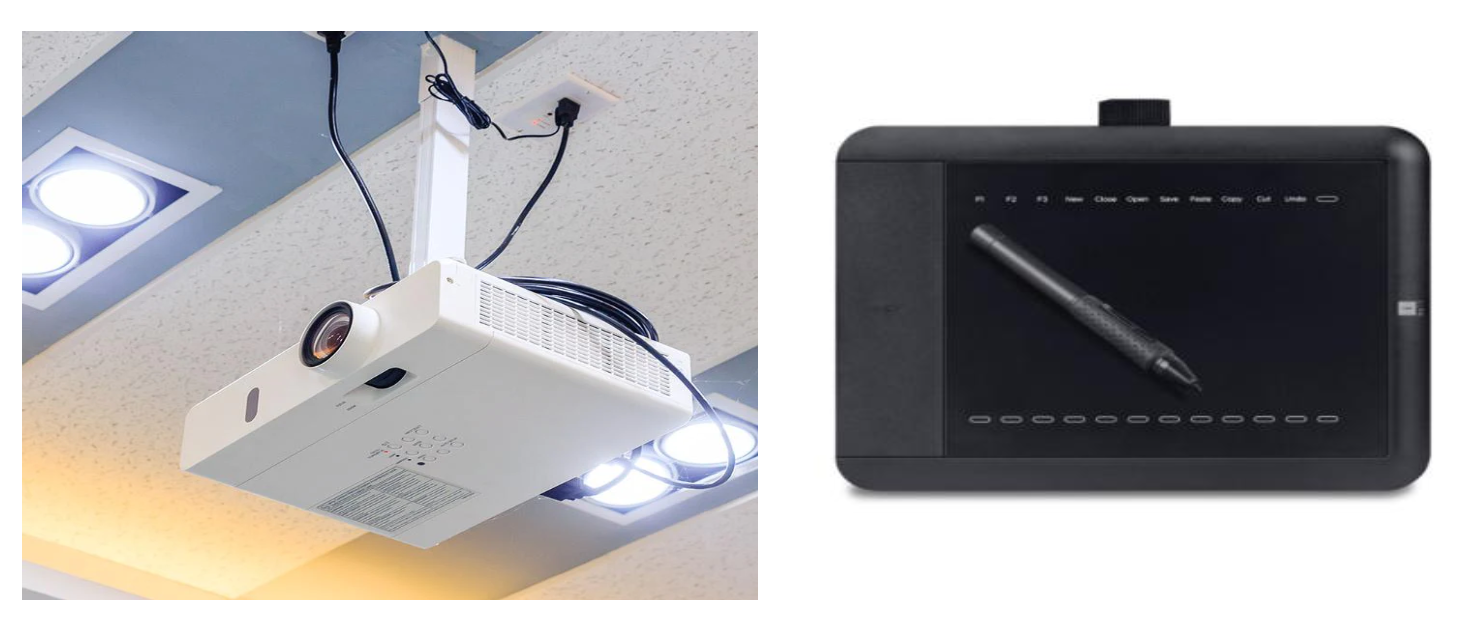
\includegraphics[width=0.85\textwidth]{images/criterion_6/media/1.png}
    \caption
    {Tools to Support Learning and Teaching.}
    \label{fig:figure1}
\end{figure}


\begin{figure}[H]
    \centering
    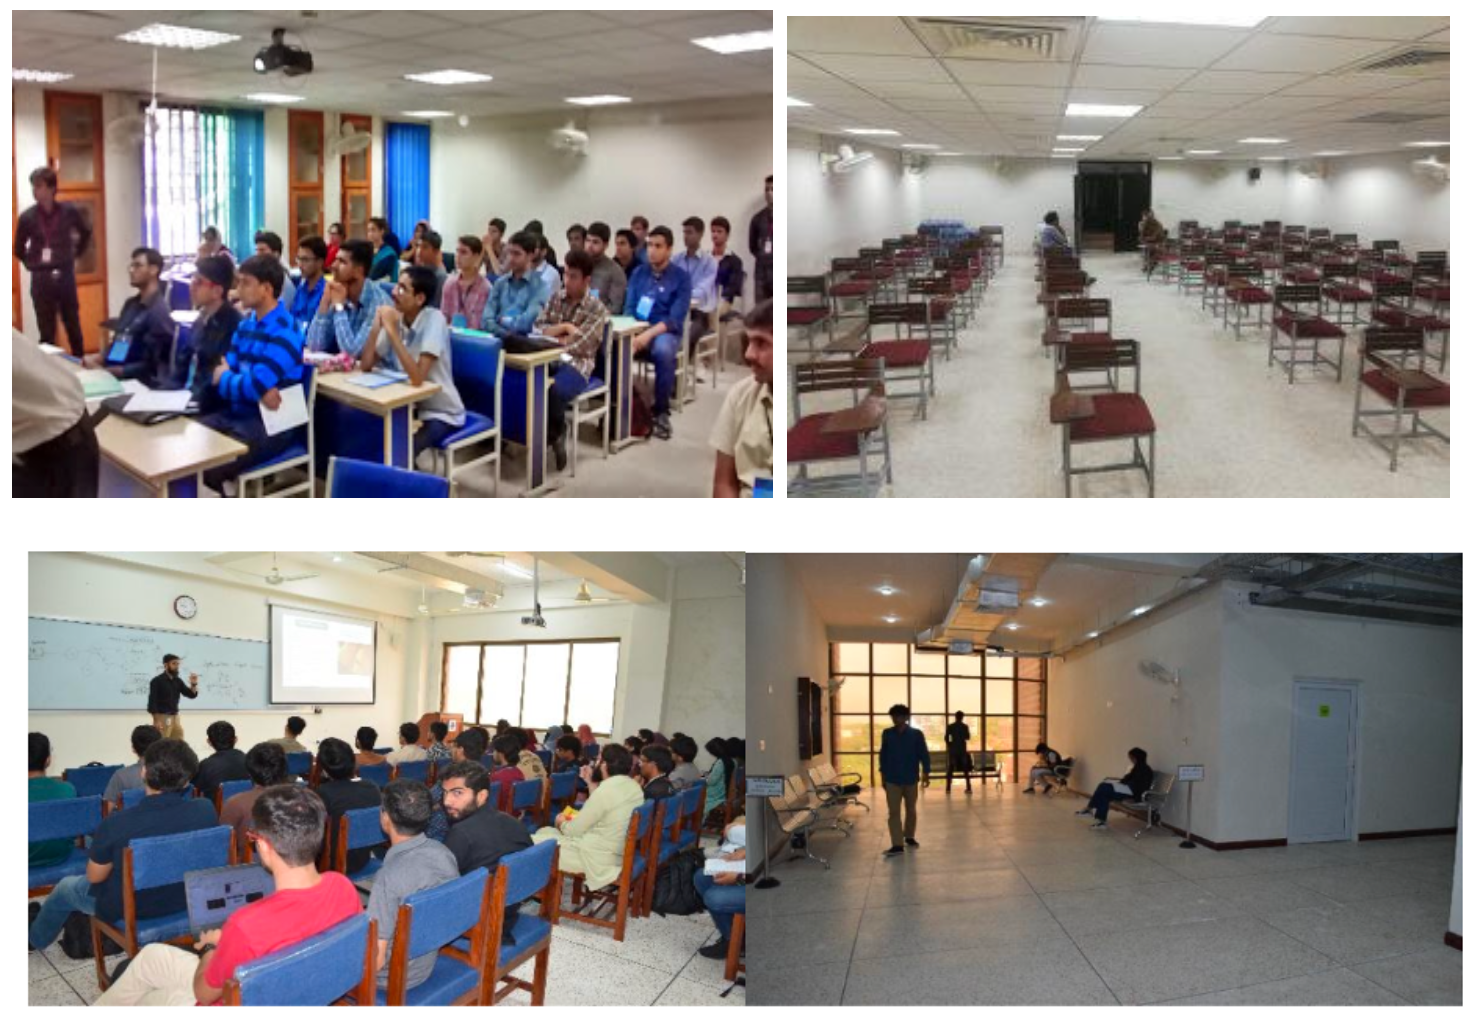
\includegraphics[width=1.0\textwidth]{images/criterion_6/media/2.png}
    \caption
    {Classrooms}
    \label{fig:figure2}
\end{figure}

\begin{table}[h]
  \centering
  \caption{SEECS infrastructure (existing blocks and New Academic Block)}
  \label{tab:infrastructure1}
  \small
  \begin{tabular}{|>{\raggedright\arraybackslash}p{0.39\textwidth}|>{\centering\arraybackslash}p{0.13\textwidth}|>{\centering\arraybackslash}p{0.15\textwidth}|>{\centering\arraybackslash}p{0.10\textwidth}|}
    \hline
    \textbf{Infrastructure} & \textbf{Existing blocks*} & \textbf{New Academic Block} & \textbf{Total} \\
    \hline
    Classrooms                            & 22      & 14      & 36       \\ \hline
    Offices -- Faculty / Officers         & 109     & 26      & 135      \\ \hline
    Principal / Assoc.\ Dean / HoD Offices & 6      & 10      & 16       \\ \hline
    Conference Rooms                      & 3       & 1       & 4        \\ \hline
    Faculty Lounges                       & 2       & 1       & 3        \\ \hline
    Common Rooms (male / female)          & 3       & 2       & 5        \\ \hline
    Exam Branch / Archive Room            & 1       & 1       & 2        \\ \hline
    Other Offices (IT/ACB/Admin/PA)       & 2/2/3/6 & 1/1/1/7 & 3/3/4/13 \\ \hline
  \end{tabular}

  \vspace{2pt}
  {\footnotesize *Existing blocks: UG/PG SEECS blocks, RIMMS and IAEC.\par}
\end{table}

\begin{figure}[H]
    \centering
    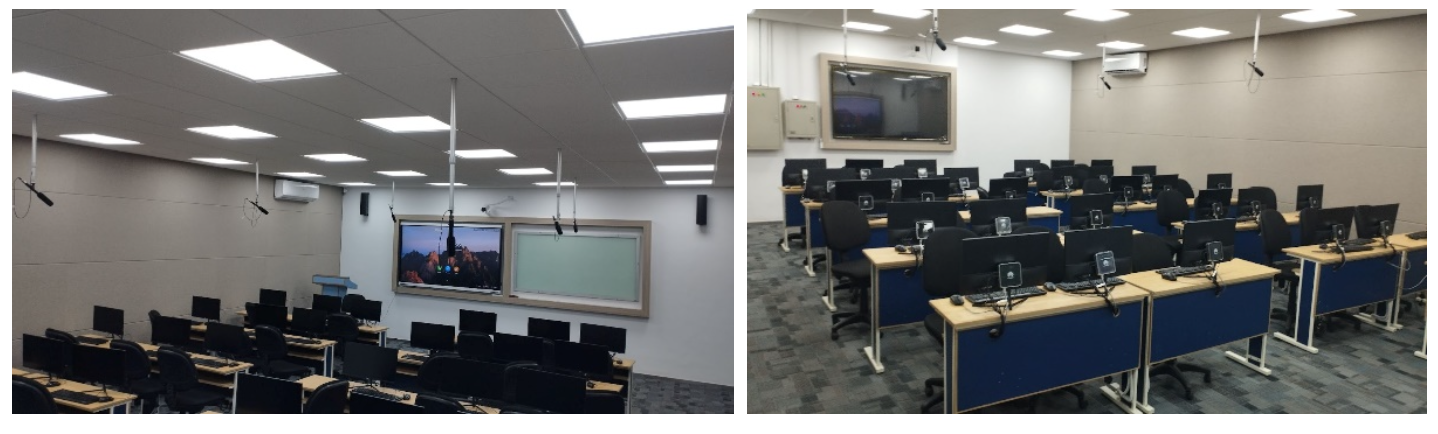
\includegraphics[width=1.0\textwidth]{images/criterion_6/media/3.png}
    \caption
    {Smart Classroom}
    \label{fig:figure3}
\end{figure}

\hypertarget{section-1}{%
% \section{\texorpdfstring{\protect\includegraphics[width=6.5in,height=2.44444in]{media/image8.png}}{}}\label{section-1}}
}

%\hypertarget{computer-facilities}{%
% \subsection{Computer Facilities}\label{computer-facilities}}

% Computer Facilities are available to all faculty members. Upon hiring, a faculty member is allocated a workstation. The equipment is upgraded as and when required depending on the requirements of the work conducted by the faculty member. 


\hypertarget{internet-facilities}{%
\subsection{Internet Facilities}\label{internet-facilities}}

Internet facility is available to all throughout the NUST campus. Internet facilities
are connected to PERN through NUST Campus Core Network with the bandwidth of
910 Mbps. NUST-SEECS also has a backup link of 7\,Mbps that is shared by some
specific research labs. The Internet at home facility is also available for those
faculty members who wish to use various resources at NUST-SEECS from their homes.
A Virtual Private Network (VPN) server is also hosted at NUST-SEECS so that faculty
can access computing resources housed at NUST-SEECS from their homes securely.
Reliable internet connectivity is available within the library to support access to
digital resources, online databases, and other academic services. Network performance
is regularly maintained to ensure uninterrupted access for students and faculty.


\hypertarget{laboratories}{%
\subsection{Laboratories}\label{laboratories}}

University lab facilities provide a range of resources to support students in their
academic pursuits. The facilities include 12 computer labs, 1 FYDP lab and 1 Basic
Electronics Lab. The computer labs are equipped with the latest hardware and
software, allowing students to access the internet, utilize specialized software,
complete assignments, or gain in-depth hands-on experience. The FYDP lab provides a
space for students to work on their final year design project, as well as receive
feedback from faculty and peers. The university lab facilities provide students with
the resources they need to succeed in their studies. The following laboratories are
available in SEECS, including teaching and research labs.

\begin{enumerate}[label=(\arabic*)]
  \item 12x Computer Labs
  \item 1x FYDP Lab (Final Year Design Projects Lab)
  \item 1x Basic Electronics Lab
  \item 11x Research Labs
\end{enumerate}

\hypertarget{computer-laboratories}{%
\subsubsection{Computing Laboratories (Teaching Laboratories)}\label{computer-laboratories}}
The institute has 12 computing laboratories and one Final Year Design Project (FYDP) Lab (Fig.~\ref{fig:figure4}). Computing Labs 1 and 2 have 48 and 51 systems installed
respectively. Computing Labs 3 to 9 on average have 40 systems, while Computing Labs 10 and 11 each have 41 systems installed. Computing Lab 12 is equipped with 35
systems, and the FYDP Computing Lab has 33 systems available for final-year project
work. Further details are provided in Annexure~\ref{annex:labs_labwork}.

\begin{figure}[htbp]
    \centering
    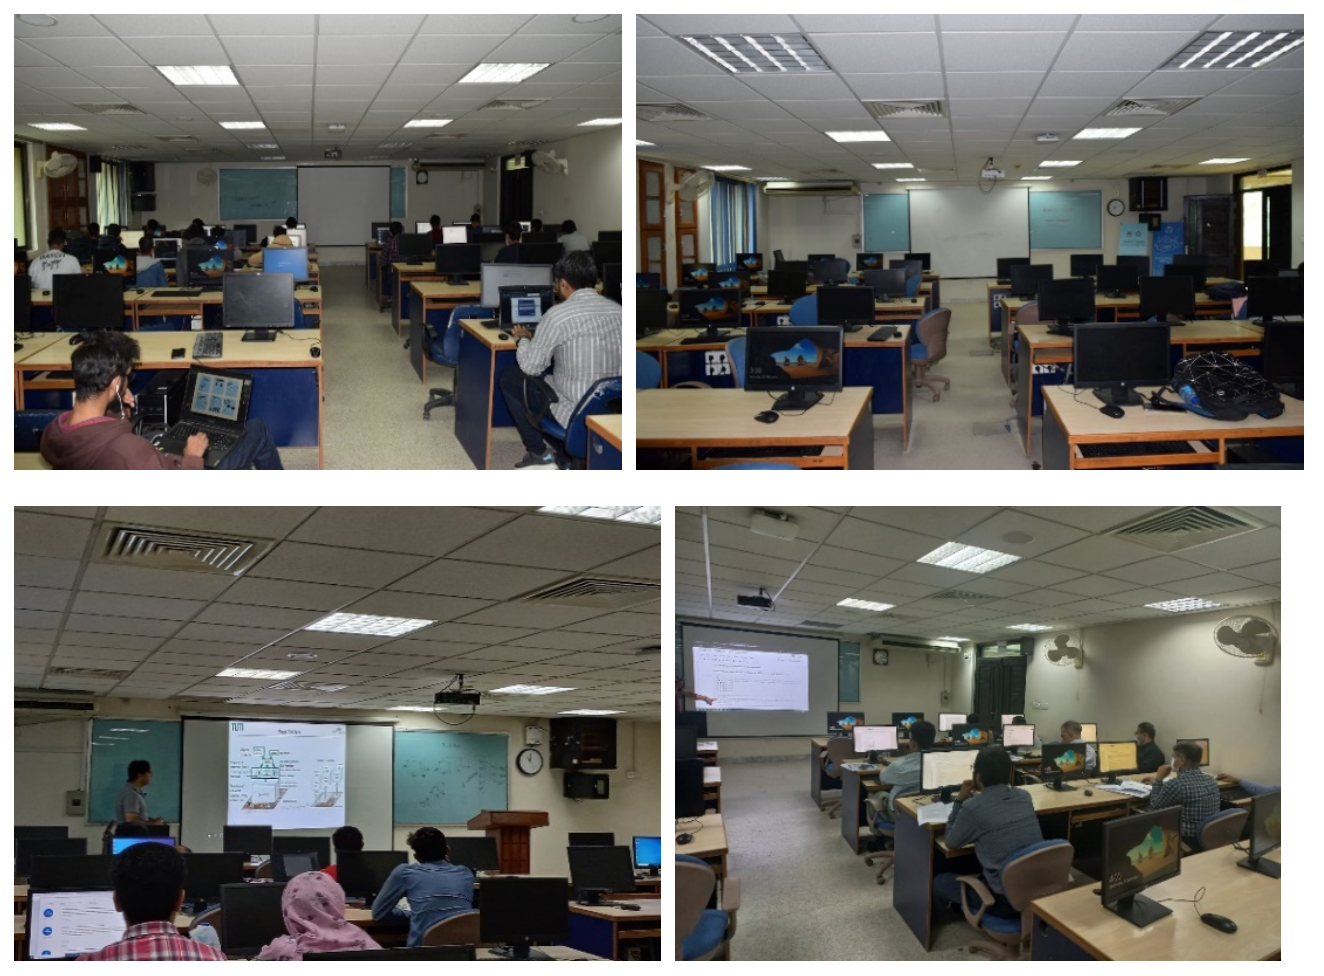
\includegraphics[width=1.0\textwidth]{images/criterion_6/media/4.png}
    \caption
    {Computer Labs}
    \label{fig:figure4}
\end{figure}


\hypertarget{research-laboratories}{%
\subsubsection{\texorpdfstring{Research Laboratories }{Research Laboratories }}\label{research-laboratories}}

The research laboratories provide a dedicated environment for conducting advanced research, experimentation, and innovation across diverse computing domains. The following research laboratories are present at SEECS:

\begin{enumerate}[noitemsep, topsep=0pt]
\def\labelenumi{(\alph{enumi})}

\item
  China-Pakistan Intelligent Systems (CPInS)

\item
  TUKL

\item
  High Performance Computing (HPC) Lab

\item
  Center for Research in Modeling, Simulation \& Vision (CRIMSON)

\item
  Knowledge-Based Systems (KBS) Lab

\item
  Walee-NUST Excellence Centre for Social \& Digital Media Technologies

\item
  Centre for Education Research and Practice (CERP)

\item
  Pak-Thai Digital Innovation Lab

\item
  Deep Learning Laboratory (DLL)

\item
  Software Modeling and Verification (SMV) Lab

\item
  NUST Staffordshire Creative AI Lab

\end{enumerate}

% New research labs such as the Internet of Things (IoT) lab and China-Pakistan Intelligent systems lab have been established after the last accreditation visit (Figure 7.5). This step has provided additional research opportunities and exposure to the UG students. We do believe in genuine improvements to fill any identified gaps. The above-stated additional facilities are substantial addition since the last accreditation visit.

% \begin{figure}[htbp]
%     \centering
%     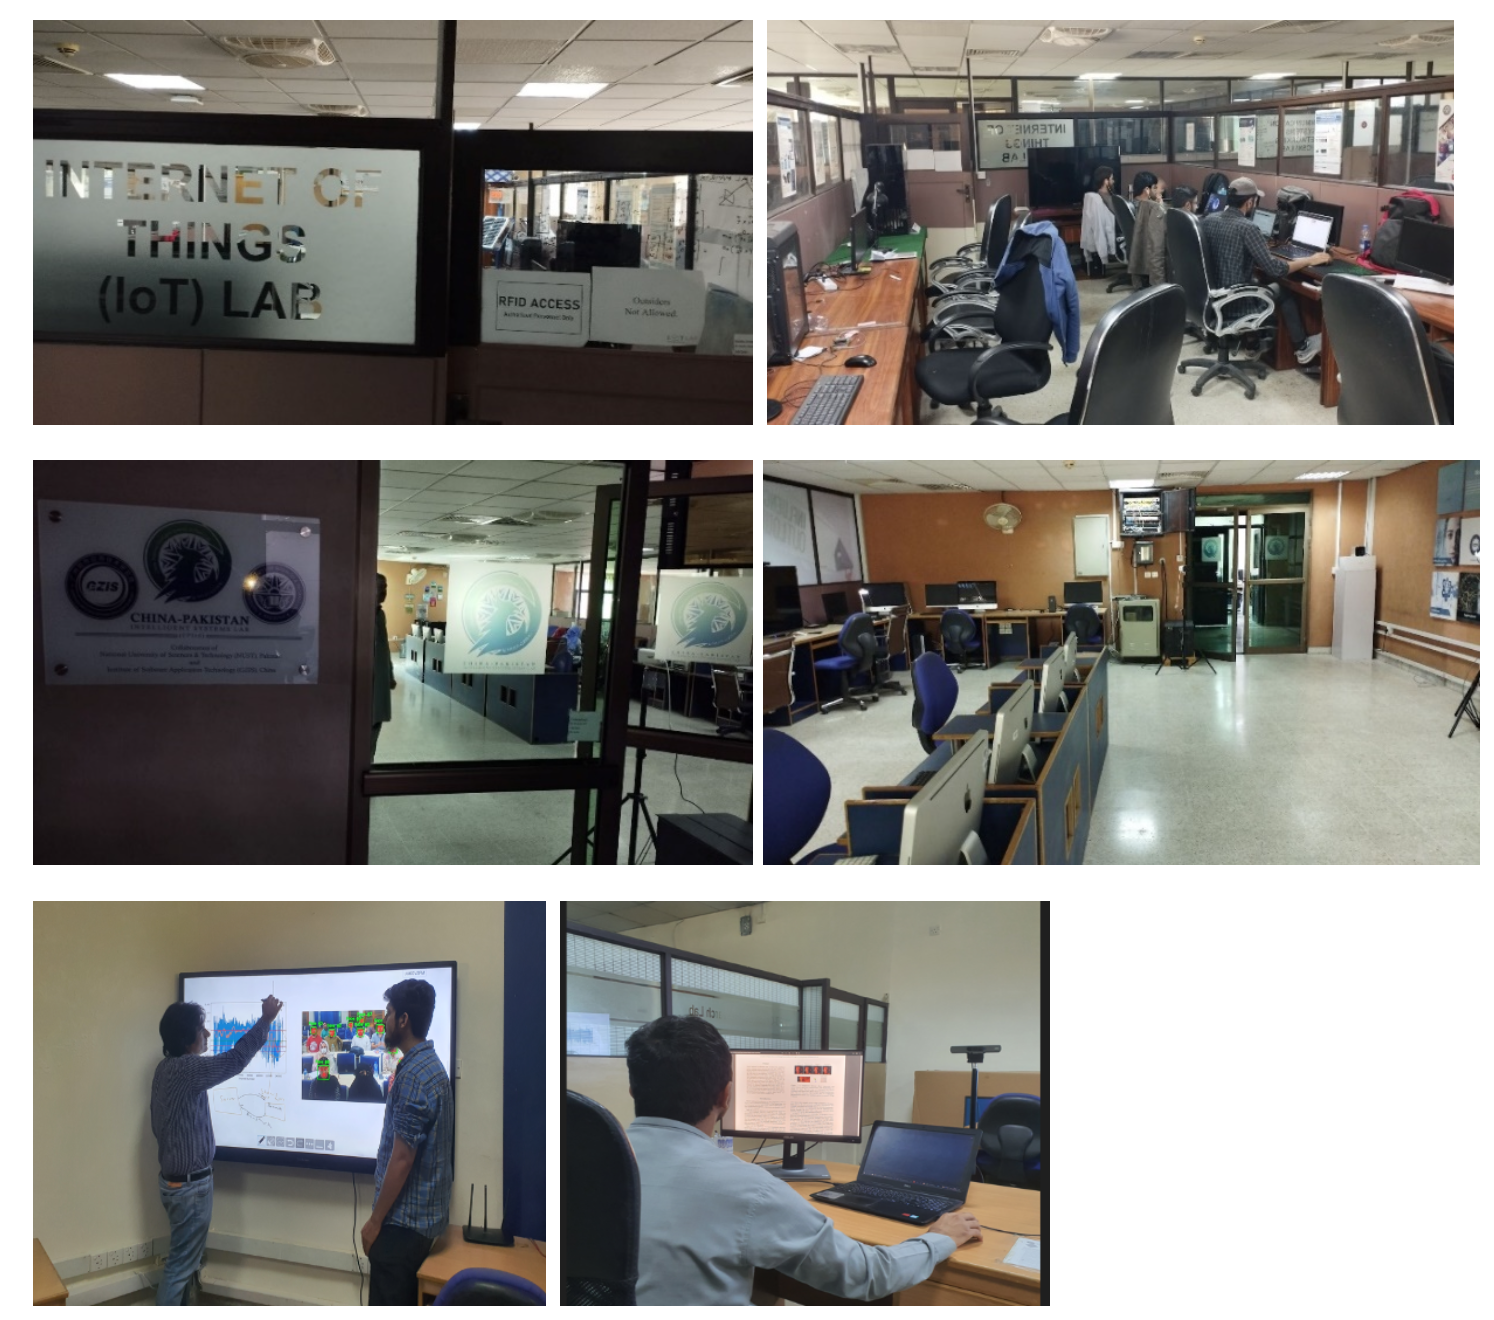
\includegraphics[width=1.0\textwidth]{images/criterion_6/media/6.png}
%     \caption
%     {Research Labs}
%     \label{fig:figure6}
% \end{figure}


\hypertarget{Conference and Seminar Halls }{%
\subsection{\texorpdfstring{Conference and Seminar Halls }{Conference and Seminar Halls }}\label{Conference and Seminar Halls}}

SEECS conference rooms and seminar halls provide a great facility for conducting
seminars, workshops, conferences, and hosting guest speakers. SEECS has 2 seminar
halls and 4 conference rooms. These rooms are equipped with the latest audio-visual
technology, comfortable seating, and ample space for large groups. They are also
equipped with whiteboards, projectors, and other necessary equipment for
presentations. Additionally, catering services are provided to attendees to ensure
that they are well-fed during the event. These rooms provide a professional and
comfortable environment for hosting events. Following seminar halls are available
at SEECS:

\begin{enumerate}
  \item SEECS (capacity 195)
  \item RIMMS (capacity 160)
\end{enumerate}

% TODO (dept): SE-SAR.xlsx says 1 of the 4 conference rooms is in the New Academic
% Block. Update the list below once the room/capacity is confirmed.
Moreover, following conference rooms are available:

\begin{enumerate}
  \item SEECS -- Faculty Block (capacity 25)
  \item SEECS -- PG Block (capacity 10)
  \item SEECS -- GRC (capacity 10)
  \item RIMMS (capacity 26)
\end{enumerate}

% \begin{figure}[htbp]
%     \centering
%     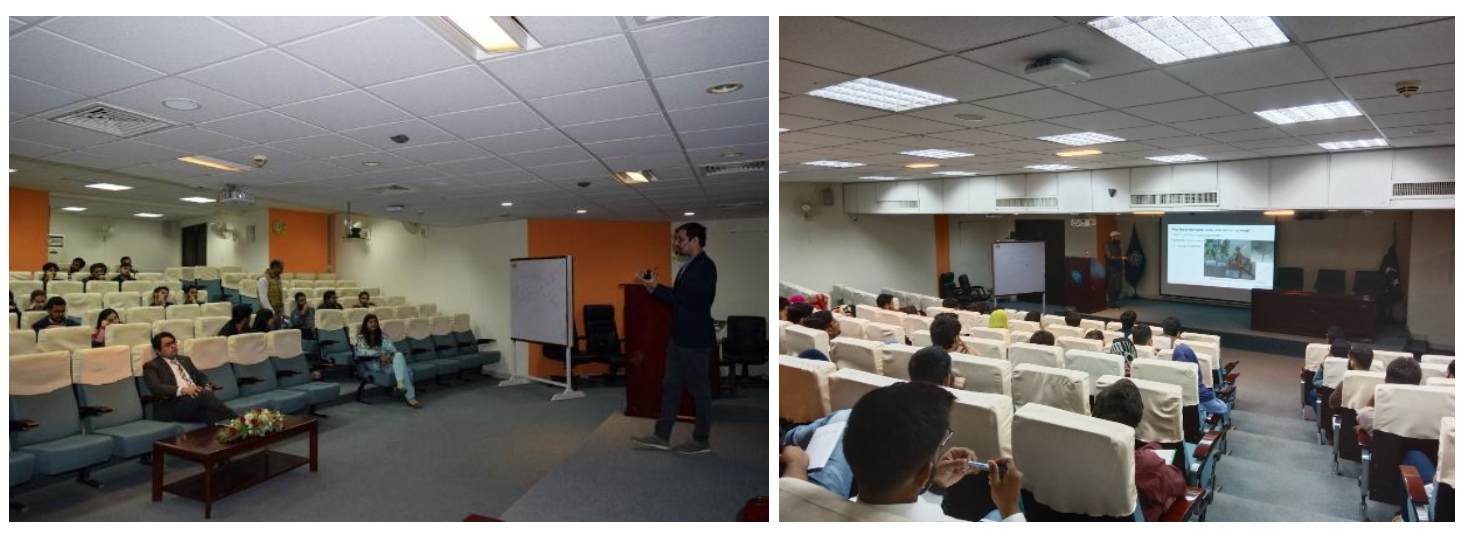
\includegraphics[width=1.0\textwidth]{images/criterion_6/media/9.png}
%     \caption
%     {Seminar Hall}
%     \label{fig:figure9}
% \end{figure}







\hypertarget{library}{%
\subsection{Library}\label{library}}

The NUST Central Library is a dynamic center of academic excellence, housing over
350,000 volumes across its main and institutional libraries. Spanning 42,907 sqft.,
this modern facility offers a serene, air-conditioned space for 570 readers,
accompanied by modern services like group study rooms, seminar halls, and cultural
hubs including the Lincoln and Chinese Corners, to support collaborative learning,
research activities, workshops, and academic events.

Spread across three floors, the library provides easy access to journals, circulation
collections, theses, and archives, empowering students, faculty, and researchers with
diverse resources to inspire learning, collaboration, and innovation. Additional
seating arrangements have been introduced to accommodate the increasing number of
library users, particularly during examination periods when daily footfall rises
significantly. To facilitate uninterrupted access to learning resources, the library
remains open seven days a week, with extended operating hours during examinations.
The University Central library facility is a comprehensive resource for students,
faculty, and staff as shown in Figure~\ref{fig:figure7}.

\begin{figure}[htbp]
    \centering
    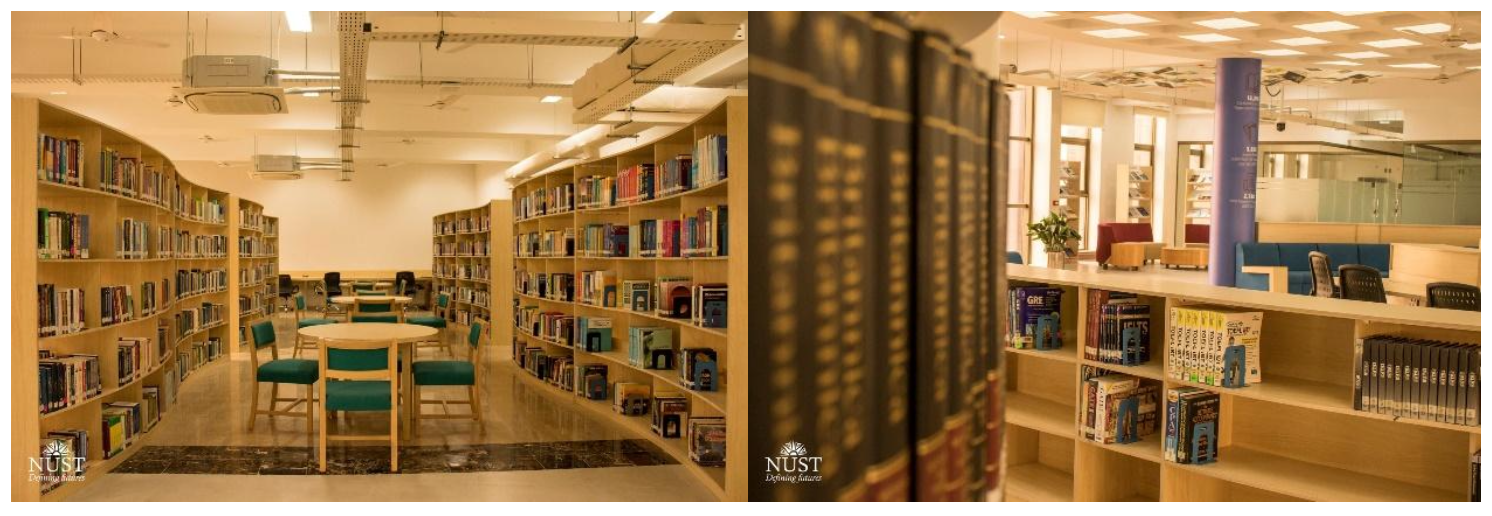
\includegraphics[width=1.0\textwidth]{images/criterion_6/media/7.png}
    \caption
    {NUST Central Library}
    \label{fig:figure7}
\end{figure}



\hypertarget{academic-library}{%
\subsubsection{Academic Library}\label{academic-library}}
The Central Library is well-equipped with an extensive collection of approximately 1,500 books related to Software Engineering and allied computing disciplines. This collection includes and is not limited to software engineering, programming, information technology, operating systems, web technologies, and data visualization. It supports the teaching, learning, and research needs of students, researchers, and faculty members.

% The collection covers a wide range of areas including software engineering principles, software design and development, software reliability, software reuse, embedded systems, programming languages, information technology, data visualization, operating systems, web technologies, and software tools. The library houses renowned titles such as Practical Software Reuse, Software Reliability Methods, Software Runaways: Monumental Software Disasters, The Java FAQ, Introduction to Information Technology, and several other reference books that support the teaching, learning, and research requirements of undergraduate and postgraduate students, researchers, and faculty members.

\subsubsection{Digital Library and Research Journals }\label{Digital ibrary}
The NUST Central library provides a seamless access to a wide range of educational resources to its faculty and students. A dedicated digital library containing a large collection of research papers, theses (23217), e-books (245), and project research archives are available through HEC. In addition to this, the central library subscribes to several other IEEE and ACM journals/magazines of international repute in hard-copy form which are readily available to the faculty and students. The university provides access to a comprehensive digital library through the Higher Education Commission (HEC), offering international research journals and scholarly databases in the domain of Software Engineering and related fields. The available resources include prestigious journals from Taylor and Francis and Wiley-Blackwell databases, including Software: Practice and Experience, Software Testing, Verification and Reliability, Journal of Software: Evolution and Process, Concurrency and Computation: Practice and Experience, Scientific Programming, Enterprise Information Systems, International Journal of Parallel, Emergent and Distributed Systems, Journal of Computer Information Systems, and Human Computer Interaction. These digital resources provide students and faculty with access to the latest advancements, research findings, and emerging trends in software engineering and computing technologies.


\subsubsection{Library Statistics }\label{library statistics}
The library provides all type of academics and research support to
students and faculty alike. Table~\ref{tab:library_inventory} provides the current inventory status.

\begingroup
\footnotesize
\setlength{\tabcolsep}{4pt}
\renewcommand{\arraystretch}{1.15}
\begin{longtable}{|>{\centering\arraybackslash}p{0.09\textwidth}|>{\raggedright\arraybackslash}p{0.53\textwidth}|>{\raggedright\arraybackslash}p{0.27\textwidth}|}
\caption{Library's current inventory}
\label{tab:library_inventory}\\
\hline
\textbf{Sr. No.} & \textbf{Item Description} & \textbf{Quantity} \\
\hline
\endfirsthead

\hline
\textbf{Sr. No.} & \textbf{Item Description} & \textbf{Quantity} \\
\hline
\endhead

1 & Total Printed Books & 44,092 \\
\hline
2 & Books on Software Engineering & 1,498 \\
\hline
3 & Online Books (HEC Subscribed) & 50,000 \\
\hline
4 & Printed Magazines & 14 \\
\hline
5 & Online Journals (HEC Subscribed) & 10 Resources (4 Basic \& 6 Premium) \\
\hline

\end{longtable}
\endgroup

\subsubsection{Library Management and Repository System}
The NUST Library System utilizes KOHA as its Integrated Library Management System (ILMS) and DSpace as its Institutional Repository platform.
Both systems are periodically upgraded and customized to improve functionality, usability, security, and system performance.
Continuous efforts are being made to enhance resource discovery and facilitate seamless access to library collections through improved system integration. Free subscription of Coursera through HEC, which includes several specializations is available for the faculty and students.

% \begin{figure}[htbp]
%     \centering
%     
\includegraphics[width=1.0\textwidth]{images/criterion_6/media/8.png}
%     \caption
%     {Online Learning Platforms: Coursera}
%     \label{fig:figure8}
% \end{figure}



\subsubsection{NUST ConnectEd – Digital Learning Platform}\label{learning-platforms}

NUST ConnectEd is an interactive online learning platform designed to provide flexible and accessible learning opportunities through both self-paced and cohort-based courses. The platform offers pre-recorded learning content along with structured courses delivered by experienced NUST faculty. Courses are supported by supplementary learning materials, resources, and assessments, enabling learners to enhance their knowledge and skills while benefiting from a flexible and engaging digital learning environment.

In addition, NUST ConnectEd offers a Career Guidance Series aimed at supporting high school and undergraduate students in making informed academic and career choices. The series features guidance from experienced professionals and industry experts across diverse disciplines, emerging technologies, higher education, and professional pathways. It also provides practical guidance on educational opportunities, including topics such as postgraduate studies and international scholarship opportunities.
NUST ConnectEd can be accessed online through the official portal\footnote{https://connected.nust.edu.pk/}.

% Apart from these, Central Library is equipped with the state-of-the-art facilities such as bookable Group Study Rooms, Seminar Hall, Conference Room, computer terminals, high speed DSL and Wi-Fi Internet access and laptop points along with electric sockets for charging.

\hypertarget{support-facilities}{%
\section{Support Facilities}\label{support-facilities}}

\hypertarget{hostels}{%
\subsection{Hostels}\label{hostels}}

NUST provides comfortable and affordable on-campus accommodation for students, faculty, and employees. Fully furnished student hostels offer dining and essential amenities that support a focused academic environment. Faculty and employee residences provide a peaceful and secure setting, with nearby recreational facilities for adults and children. Figure~\ref{fig:figure10} shows the boys’ hostel building and rooms. NUST also offers dining facilities within hostels and faculty and officer accommodations. Cafeterias and tuck shops are located near academic buildings, offices, gymnasia, and residential blocks, while dedicated messes serve daily meals to faculty and officers.
Alongside campus-wide security, all hostels have protective boundary walls, security personnel, and dedicated staff. Each male and female hostel block is supervised by a hostel manager and a resident caretaker available around the clock.

\hypertarget{hostel-facilities}{%
\subsubsection{Hostel Facilities}\label{hostel-facilities}}

\begin{enumerate}[itemsep=1pt, topsep=2pt, parsep=0pt]
\item Fully furnished accommodation
\item Cubical / Bi-seater rooms with attached washroom
\item Bi-seaters / Tri-seater rooms with community Washroom
\item TV Room
\item Well-equipped Mess in each hostel
\item Laundry
\item Gymnasium
\item Badminton courts
\item Table Tennis
\item Billiard Board
\item Vending Machine
\item Electric Oven and Iron
\item Internet facility
\item Radiator Heating System
\item Medical cover for 24 hours
\item Shuttle service on Holidays
\end{enumerate}

\hypertarget{hostel-accommodation}{%
\subsubsection{Hostel Accommodation}\label{hostel-accommodation}}

Hostel Accommodation in the relevant category is strictly allotted according to the application seniority list. Hostels are well-maintained and provide all necessary facilities to make the students comfortable (Figure~\ref{fig:figure10}). The separately located hostels for males and females have been named after great Muslim scholars, as under:

\noindent\textbf{Hostels for Male Students}

\begin{enumerate}[itemsep=1pt, topsep=3pt, parsep=0pt]
    \item Rumi Hostels Block-I, II \& III -- PG Students
    \item Ghazali Hostels Block-I \& II -- UG Students
    \item Razi Hostels Block-I \& II -- UG Students
    \item Attar Hostels Block-I \& II -- UG Students
    \item Hajveri Hostel -- UG Students
    \item Zakariya Hostel -- UG Students
\end{enumerate}

\noindent\textbf{Hostels for Female Students}

\begin{enumerate}[itemsep=1pt, topsep=3pt, parsep=0pt]
    \item Fatima Hostels Block-I \& II -- PG Students
    \item Zainab Hostel -- UG Students
    \item Ayesha Hostel -- UG Students
    \item Khadija Hostel -- UG Students
    \item Amna Hostel -- UG Students
\end{enumerate}


%\textbf{Note}:~National UG Students in 1st to 3rd Semester will be allocated tri-seater accommodation in the hostels. 

% Annex AI contains more details on hostel facilities (Appendix~\ref{}).

\begin{figure}[htbp]
    \centering
    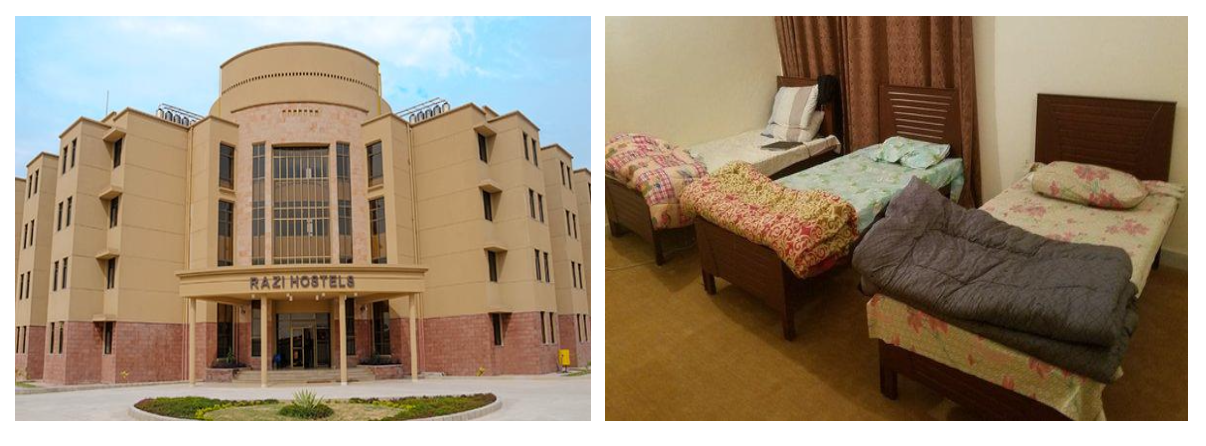
\includegraphics[width=1.0\textwidth]{images/criterion_6/media/10.png}
    \caption
    {Students hostel accommodation}
    \label{fig:figure10}
\end{figure}


\hypertarget{common-areas}{%
\subsection{Common Areas}\label{common-areas}}

By providing a comfortable and inviting atmosphere, common rooms can help foster a
sense of community among students and encourage them to stay connected with their
peers. SEECS offers a total of 5 common rooms which are equipped with comfortable
seating and tables. These spaces provide a place for students to socialize, study,
and take a break from their academic responsibilities.



\hypertarget{fitness-rooms}{%
\subsection{Fitness Rooms}\label{fitness-rooms}}

University fitness rooms provide students with access to a variety of exercise equipment and activities to help them stay healthy and fit. Fitness room is available at SEECS which includes a variety of cardio machines, strength training equipment, and free weights. The goal of SEECS fitness room is to provide students with the resources they need to maintain a healthy lifestyle.



\hypertarget{health-center}{%
\subsection{Health Center}\label{health-center}}

% On-campus medical facilities for students and staff is the most important service a university must provide to ensure the health and well-being of its employees and students. NUST Medical Centre provides health services, including 24/7 outpatient medical care for students and staff completely free of cost for everyone on campus. It also arranges inpatient medical cover in affiliated hospitals, while promoting activities for general wellbeing of NUST community (Figure 7.10).

% The medical center consists of at least two on-duty medical officers, nurses, staff, and round-the-clock emergency health-care services with ambulances. These free of cost medical facilities are available on all the seven campuses of NUST all over Pakistan. Other than these facilities, health insurance for staff and students has also been provided through subsidized insurance packages.

NUST Medical Centre provides free, 24/7 outpatient and emergency care for students and staff, supported by medical officers, nurses, and ambulance services. It also arranges inpatient care at affiliated hospitals and promotes community well-being (Figure~\ref{fig:figure11}).
Free medical services are available across all seven NUST campuses in Pakistan, complemented by subsidized health insurance packages for students and staff.
\begin{figure}[htbp]
    \centering
    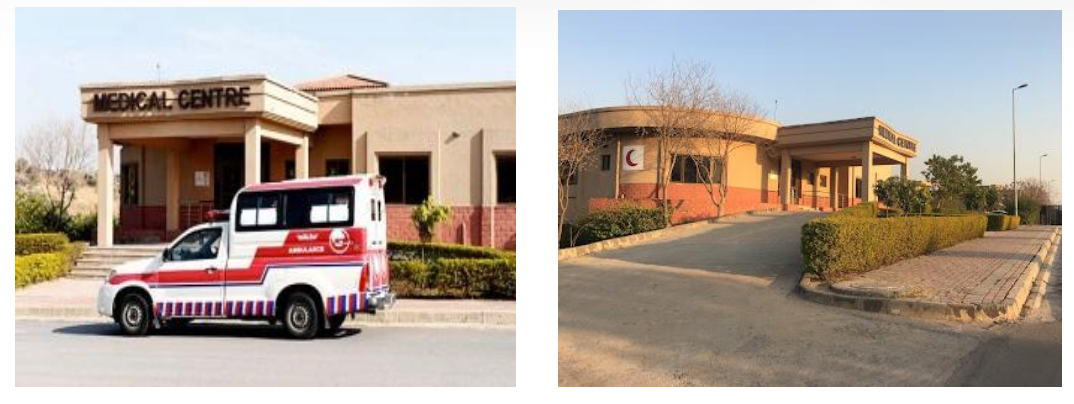
\includegraphics[width=1.0\textwidth]{images/criterion_6/media/11.png}
    \caption
    {NUST Medical Center (NMC)}
    \label{fig:figure11}
\end{figure}

\hypertarget{student-center}{%
\subsection{Student Center}\label{student-center}}

% The Student Center operates under the auspices of Student Affairs Directorate. The Center renders multiple services to NUST students as delineated below:

% \begin{enumerate}
% \def\labelenumi{\arabic{enumi}.}
% \item
%   Coordinates/ facilitates activities of all the University Clubs and Societies. The conduct of co-curricular activities through these forums enables students to enhance their mental abilities and prepare themselves for the daunting challenges of the future.
% \item
%   Runs a publications section comprising a team of editors and student editors, for publishing the University's monthly newsletter - NUSTNEWS, the annual bilingual literary magazine -- THE NUSTIAN, and a yearly publication NUSTXTRA, which exclusively covers both on- and off-campus co-curricular activities of the students. The Publications section also keeps liaison with HEC Publications Directorate for proper coverage of NUST events in its publications such as HEC newsletter- News \& Views. In addition to this, the publications department also covers the University events for publishing in the national and international press.
% \item
%   Houses a Fiction Library with a rich collection of literary works in both Urdu and English languages. The students enjoy leisure time from their tough academic routines, reading books of their choices. These books give them an insight into different meanings of and perspectives on life through the prism of veritable intellectual masterpieces.
% \item
%   Deals with discipline matters of students, as and when referred to student affairs (SA) Directorate by NUST institutions. Director Student Affairs heads the Discipline Committee.
% \item
%   Acts as a Front Office for processing all student related affairs/ queries, i.e., degrees, transcripts, refunds, scholarships etc.
% \item
%   Houses the Secretariat of Pakistan Chapter of The Talloires Network, PCTN. The Chapter promotes civic engagement in the higher education sector of Pakistan.
% \item
%   Provides facilities such as cafeteria, mini mart, stationery etc.
% \end{enumerate}


The Student Center operates under the Student Affairs Directorate renders multiple services to NUST students as delineated below:
\begin{enumerate}[noitemsep, topsep=0pt]
\item Coordinates university clubs, societies, and co-curricular activities to support students’ personal development and preparation for future challenges.

\item Manages university publications, including the monthly newsletter NUSTNEWS, the annual bilingual literary magazine THE NUSTIAN, and NUSTXTRA, which covers student co-curricular activities. It also coordinates coverage of university events in HEC publications and the national and international press.

\item Houses a Fiction Library offering Urdu and English literary works for leisure reading and intellectual enrichment.

\item Handles student disciplinary matters referred by NUST institutions, with the Director Student Affairs heading the Discipline Committee.

\item Serves as a front office for student queries and matters related to degrees, transcripts, refunds, and scholarships.

\item Houses the Secretariat of the Pakistan Chapter of the Talloires Network (PCTN), which promotes civic engagement in Pakistan’s higher education sector.

\item Provides amenities, including a cafeteria, mini mart, and stationery facilities.
\end{enumerate}

\subsection{NUST Student Support Services Centre (S3C)}
NUST Student Support Services Centre (S3C) is a new initiative which is centralized, one-window facilitation platform designed to streamline student requests and support services across campus.



\begin{enumerate}[noitemsep, topsep=0pt]
    \item \textbf{Student Help Desk}
    \begin{itemize}
        \item \textbf{Primary Function:} General queries, campus life facilitation, and academic enrollment assistance.
  %      \item \textbf{Phone Numbers:} \\+92-51-90851689 \textbar\ +92-51-90851699
  %      \item \textbf{Email:} \texttt{studenthelpdesk@nust.edu.pk}
    \end{itemize}

    \item \textbf{Center for Counseling and Career Advisory (C3A)}
    \begin{itemize}
        \item \textbf{Primary Function:} Professional mental health counselling, personal development workshops, and career guidance.
    \end{itemize}

    \item \textbf{Hostel Management}
    \begin{itemize}
        \item \textbf{Primary Function:} On-campus lodging, room allocations, and residential student affairs.
    %    \item \textbf{Male Hostels (Assistant Director):} +92-51-90851509
    %    \item \textbf{Female Hostels (Assistant Director):} +92-51-90851527
    \end{itemize}

    \item \textbf{Fee Affairs}
    \begin{itemize}
        \item \textbf{Primary Function:} Tuition management, installment schedules, and fee refund processing.
    \end{itemize}
\end{enumerate}

\subsection{Centre for Counselling and Career Advisory (C3A)}

The Centre for Counselling and Career Advisory (C3A) provides professional counselling services to support the mental health and well-being of NUST students, faculty, staff, and their families. The centre offers confidential counselling for educational, social, emotional, and psychological concerns that may affect personal or professional development. C3A is staffed by qualified psychologists and counsellors who provide individual and group counselling, consultation services, psychological assessments, psycho-educational programmes, training sessions, and workshops. Standardized psychological assessments, including Intelligence Quotient (IQ), Emotional Quotient (EQ), personality, aptitude, career interest, stress, anxiety, and depression tests, are available to promote the overall well-being and personal development of the university community.

\subsection{Career Development Centre (CDC)}

The Career Development Centre (CDC) is dedicated to enhancing students' employability by developing the professional and interpersonal skills required in today's competitive job market. The centre offers career development programmes, training modules, networking events, career counselling, employer engagement activities, curriculum support, and co-curricular initiatives to bridge the gap between academic learning and industry requirements. Through close collaboration with employers and the NUST Placement Office, the CDC equips students with the competencies necessary for successful career planning, employment, and professional growth.


\hypertarget{sport-and-recreational-facilities}{%
\section{Sports and Recreational Facilities}\label{sport-and-recreational-facilities}}

NUST affords an array of sports and other recreational facilities to its students, faculty, and staff. Sports infrastructure includes athletic tracks; cricket, hockey, and football grounds; various indoor sports facilities; gymnasia, etc. NUST has also recently established Pakistan's first university-based Horse-Riding Club and a one-of-a-kind Sports Complex, which includes swimming, archery, basketball, badminton, tennis, bowling, and other sports (Figure~\ref{fig:figure12}). The purpose of establishing such a facility is to invoke the urge for a healthy lifestyle among the NUST community, including students, alumni, faculty, staff, and their families. Moreover, there are also 80+ student-led Clubs and Societies across all campuses that inspire students to display and refine their dynamic literary, creative, and artistic abilities and aptitudes in the company of like-minded individuals.

\begin{figure}[htbp]
    \centering
    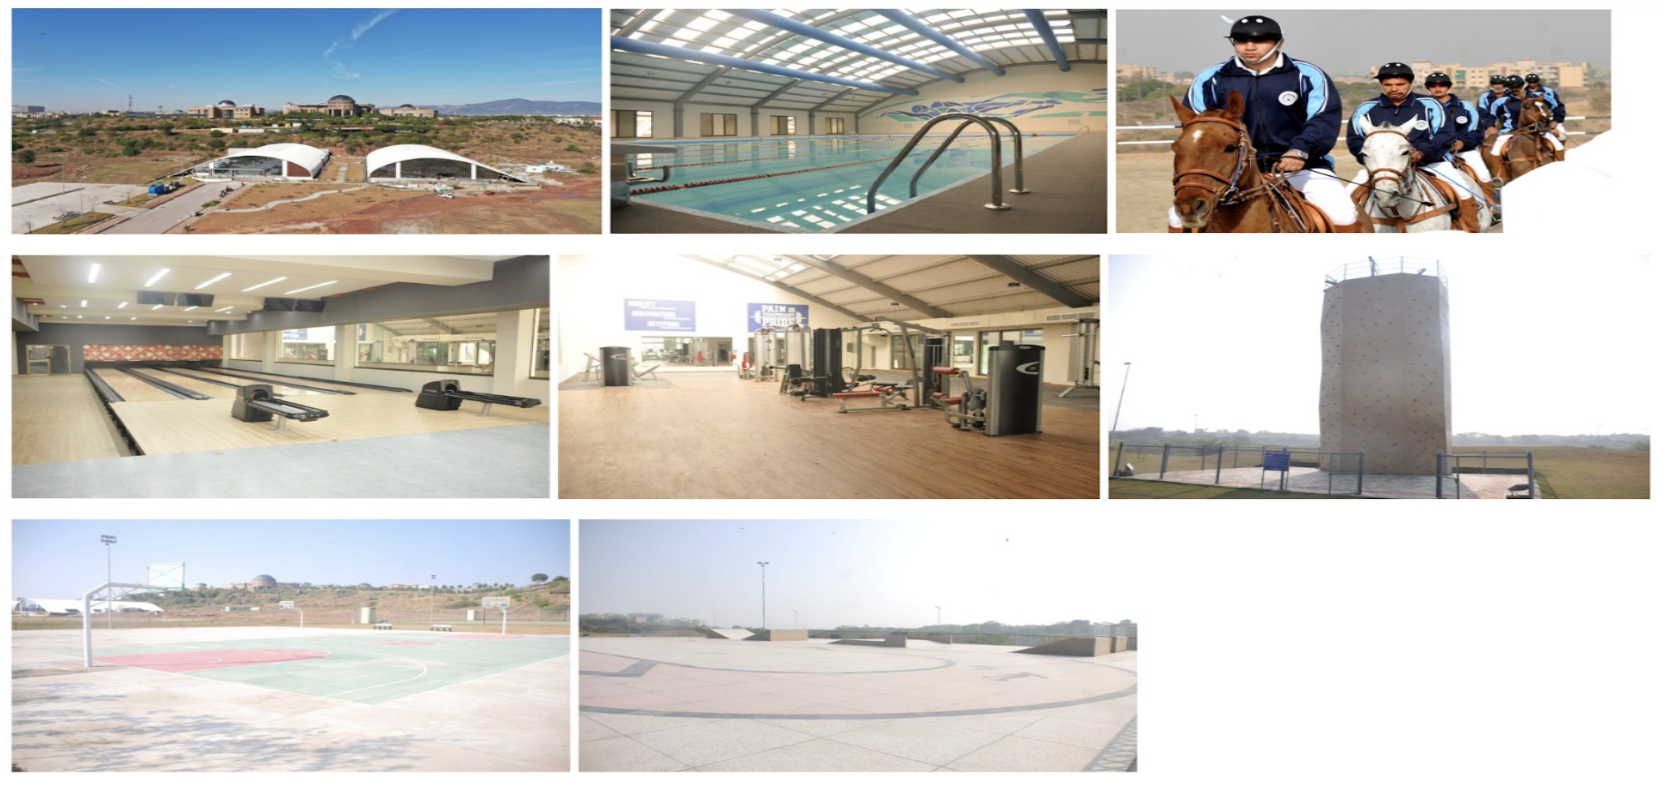
\includegraphics[width=1.0\textwidth]{images/criterion_6/media/12.png}
    \caption
    {Sports and recreational facilities}
    \label{fig:figure12}
\end{figure}


\hypertarget{cafes}{%
\subsection{Cafes}\label{cafes}}

Aesthetically designed cafeterias and shopping complex (Concordia I and Concordia II) have been constructed in the northern and southern wings of the campus (Figure~\ref{fig:figure13}). The cafeteria provides an opportunity to the students to relax and enjoy their snacks and meals in a hygienic environment. Each shopping complex offers the following services:
\begin{itemize}[itemsep=1pt, topsep=2pt, parsep=0pt]
    \item Cafeteria
    \item Mini Mart
    \item Photo Shop
    \item Barber Shop
    \item Ladies' Shop (including Parlor)
    \item Computer Hardware Shop
    \item Cellular Shop
    \item Business Center Services
    \item Stationery Shop
    \item Dining/Function Halls
\end{itemize}

\begin{figure}[htbp]
    \centering
    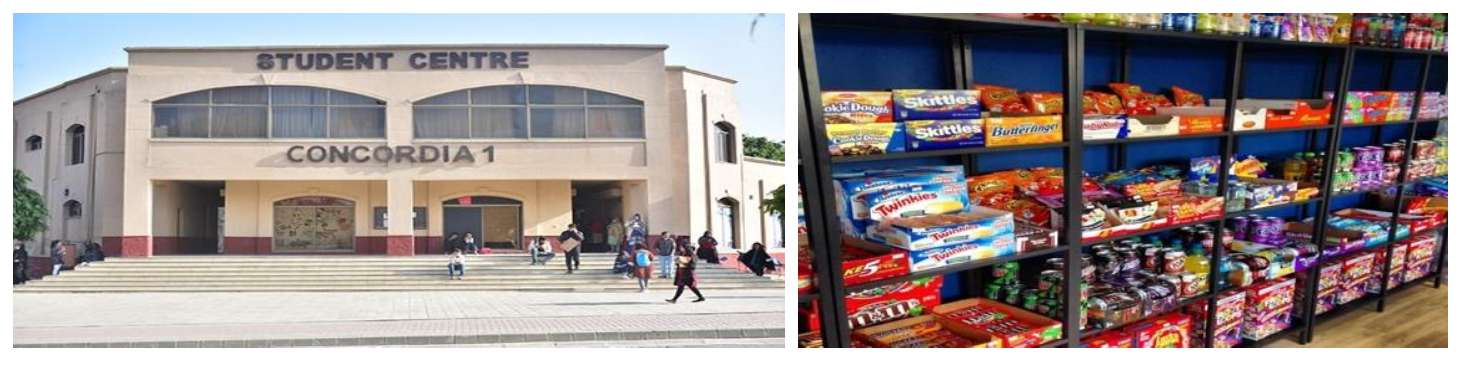
\includegraphics[width=1.0\textwidth]{images/criterion_6/media/13.png}
    \caption
    {Students cafeterias and tuck shops
}
    \label{fig:figure13}
\end{figure}


% \begin{figure}[htbp]
%     \centering
%     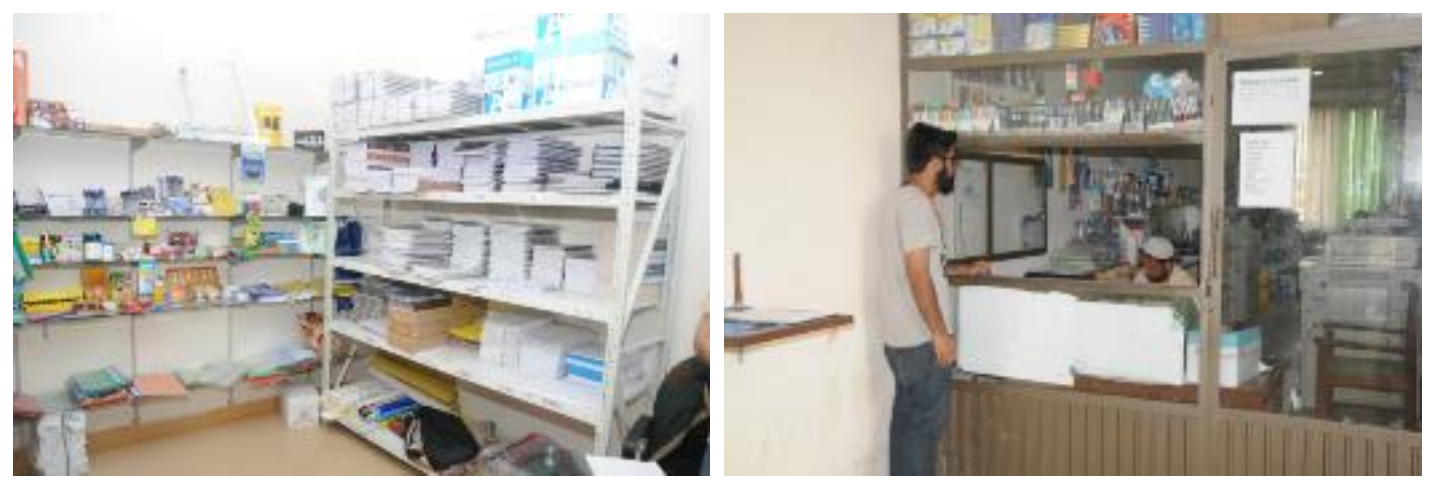
\includegraphics[width=1.0\textwidth]{images/criterion_6/media/14.png}
%     \caption
%     {Students café stationery shop
% }
%     \label{fig:figure14}
% \end{figure}


\hypertarget{transport-facilities}{%
\subsection{Transport Facilities}\label{transport-facilities}}

NUST has an elaborate and well-organized transport system to meet the requirements of students, faculty, and staff as shown in Figure~\ref{fig:figure15}. Special emphasis is on the environmentally friendly transport system. NUST runs a fleet of electric cars within its campus to minimize carbon emission. Electric cars are used as shuttle service between various locations within the campus, i.e., hostels to various School/Offices and from Gates to Schools/Hostels/Offices. NUST also has an elaborate transport system for pick and drop of students, faculty, and staff from all localities of the city with variable timings. Transport is also made available to facilitate students for industrial visits, research projects, club activities, society/community initiatives, awareness walks and excursion trips.

\begin{figure}[htbp]
    \centering
    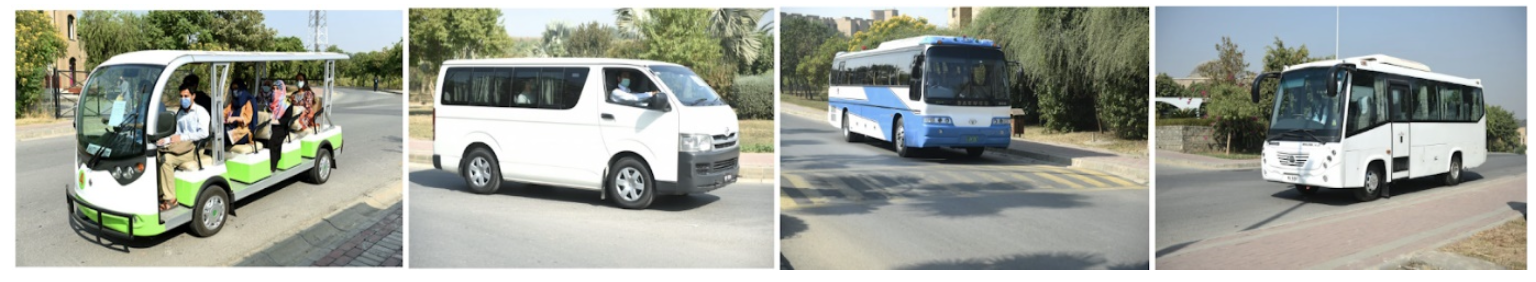
\includegraphics[width=1.0\textwidth]{images/criterion_6/media/15.png}
    \caption
    {NUST Transport Facility
}
    \label{fig:figure15}
\end{figure}


\subsection{Clubs and Societies}

With 44 clubs and societies, comprehensive sports facilities, recreational activities, and mega events, NUST provides students with opportunities to grow, explore, and experience life beyond academics. These activities not only offer a healthy balance to academic life but also encourage leadership, teamwork, and community engagement.

The major clubs and recreational facilities at NUST include:

\begin{itemize}[itemsep=1pt, topsep=2pt, parsep=0pt]
    \item NUST Bowling Alley
    \item NUST Horse Riding Club
    \item NUST Gyms and Swimming Pool
    \item NUST Hiking, Wall Climbing \& Excursion Club
    \item NUST Archery \& Pistol Club
    \item NUST Social Events and Societies
    \item NUST Community Services Club
\end{itemize}

Some of the main clubs and student organizations at SEECS are:

\begin{itemize}[itemsep=1pt, topsep=2pt, parsep=0pt]
    \item NUST Fitness Club (NFS)
    \item NUST Excursion Club (NXC)
    \item NUST Entrepreneurs Club (NEC)
    \item Institute of Electrical and Electronics Engineers (IEEE) Student Branch
    \item NUST Hack Club (NHC)
    \item Student Government Association (SGA)
    \item Graduate \& Professional Student Government (GPSG)
    \item Association for Computing Machinery (ACM)
    \item Youth Entrepreneurial Society (YES)
    \item International Association for the Exchange of Students for Technical Experience (IAESTE)
    \item Youth Impact SEECS Chapter
    \item Computer Society of Pakistan (CSP)
\end{itemize}



\hypertarget{workplace-safety}{%
\section{Workplace Safety}\label{workplace-safety}}

Health and safety are a top priority for the department and strict workplace safety regulations are followed to ensure a safe environment for all. Safe laboratory practices require a safety-conscious attitude, knowledge of hazards, and awareness of their presence. It is a shared responsibility that requires full cooperation from everyone in the workplace, including students, instructors, and researchers who must follow safety precautions and procedures. Safety instructions and evacuation plans are prominently displayed, and students receive regular briefings. The department ensures that necessary safety equipment is readily available and in good working order. Users are also trained in the location and use of safety facilities such as fire extinguishers, showers, and emergency exit, as well as familiarizing themselves with safety precautions, procedures, potential hazards, and emergency procedures.


\subsection{Work, Health and Safety}

To promote a safe and healthy working environment, SEECS has implemented a Work, Health and Safety (WHS) induction programme for all new faculty members, staff, research students, visitors, and affiliates associated with the School. The induction familiarizes participants with the University's health and safety policies, emergency procedures, reporting mechanisms, and workplace responsibilities. In addition, at least one WHS awareness and training session is conducted every semester for faculty and staff to reinforce safe work practices and ensure compliance with institutional policies and national occupational safety requirements.

The key topics covered during the induction and training sessions include:

\begin{enumerate}
  \item General Work, Health and Safety (WHS) responsibilities in accordance with the
        University Policy.
  \item Procedures for reporting incidents, injuries, illnesses, and workplace hazards.
  \item Local consultation arrangements for WHS matters through the School Safety
        Committee.
  \item Contact information for Safety Officers, First Aid Officers, and Building
        Wardens.
  \item Contact details are provided for reporting maintenance issues relating to
        buildings and grounds using the University Web Help Desk/ICT and other
        portals\footnote{\url{https://seecs.nust.edu.pk/contact/}}.
  \item Overview of occupational safety and health (OSH) legislation and relevant
        safety regulations applicable in Pakistan.
\end{enumerate}

NUST also follows a university wide University Health, Safety and Environment Policy. 
Detailed guidelines of university policy and SEECS health and safety induction checklist are available in Appendix~\ref{annex:NUST healthsafetypolicy} and Appendix~\ref{annex:work health safety checklist} respectively.

\hypertarget{fire-safety}{%
\subsection{Fire Safety}\label{fire-safety}}

The administration is dedicated to providing and maintaining a safe and healthy work environment. A standard operating procedure (SOP) has been established to handle fire emergencies which includes the following measures:

\begin{enumerate}[noitemsep, topsep=0pt]
\item Designation of a Fire Safety Officer for SEECS.
\item Designation of Fire Marshals for each floor of the building.
\item Installation of a fire alarm system.
\item Availability of 26 fire extinguishers and first aid boxes throughout the institute's building.
\item Posting of evacuation plans at prominent locations, offices, and classrooms.
\item Two emergency exit doors on each floor for safe evacuation.
\item Clearly marked assembly points outside the building.
\item Display of emergency contact numbers on noticeboards.
\item Availability of the NUST Medical Centre and Fire Department on campus to respond to emergencies.
\item Fire-fighting drills conducted every semester to enhance the awareness and preparedness of students and staff (Figure~\ref{fire_drill}).
\end{enumerate}

\begin{figure}[t]
    \centering
    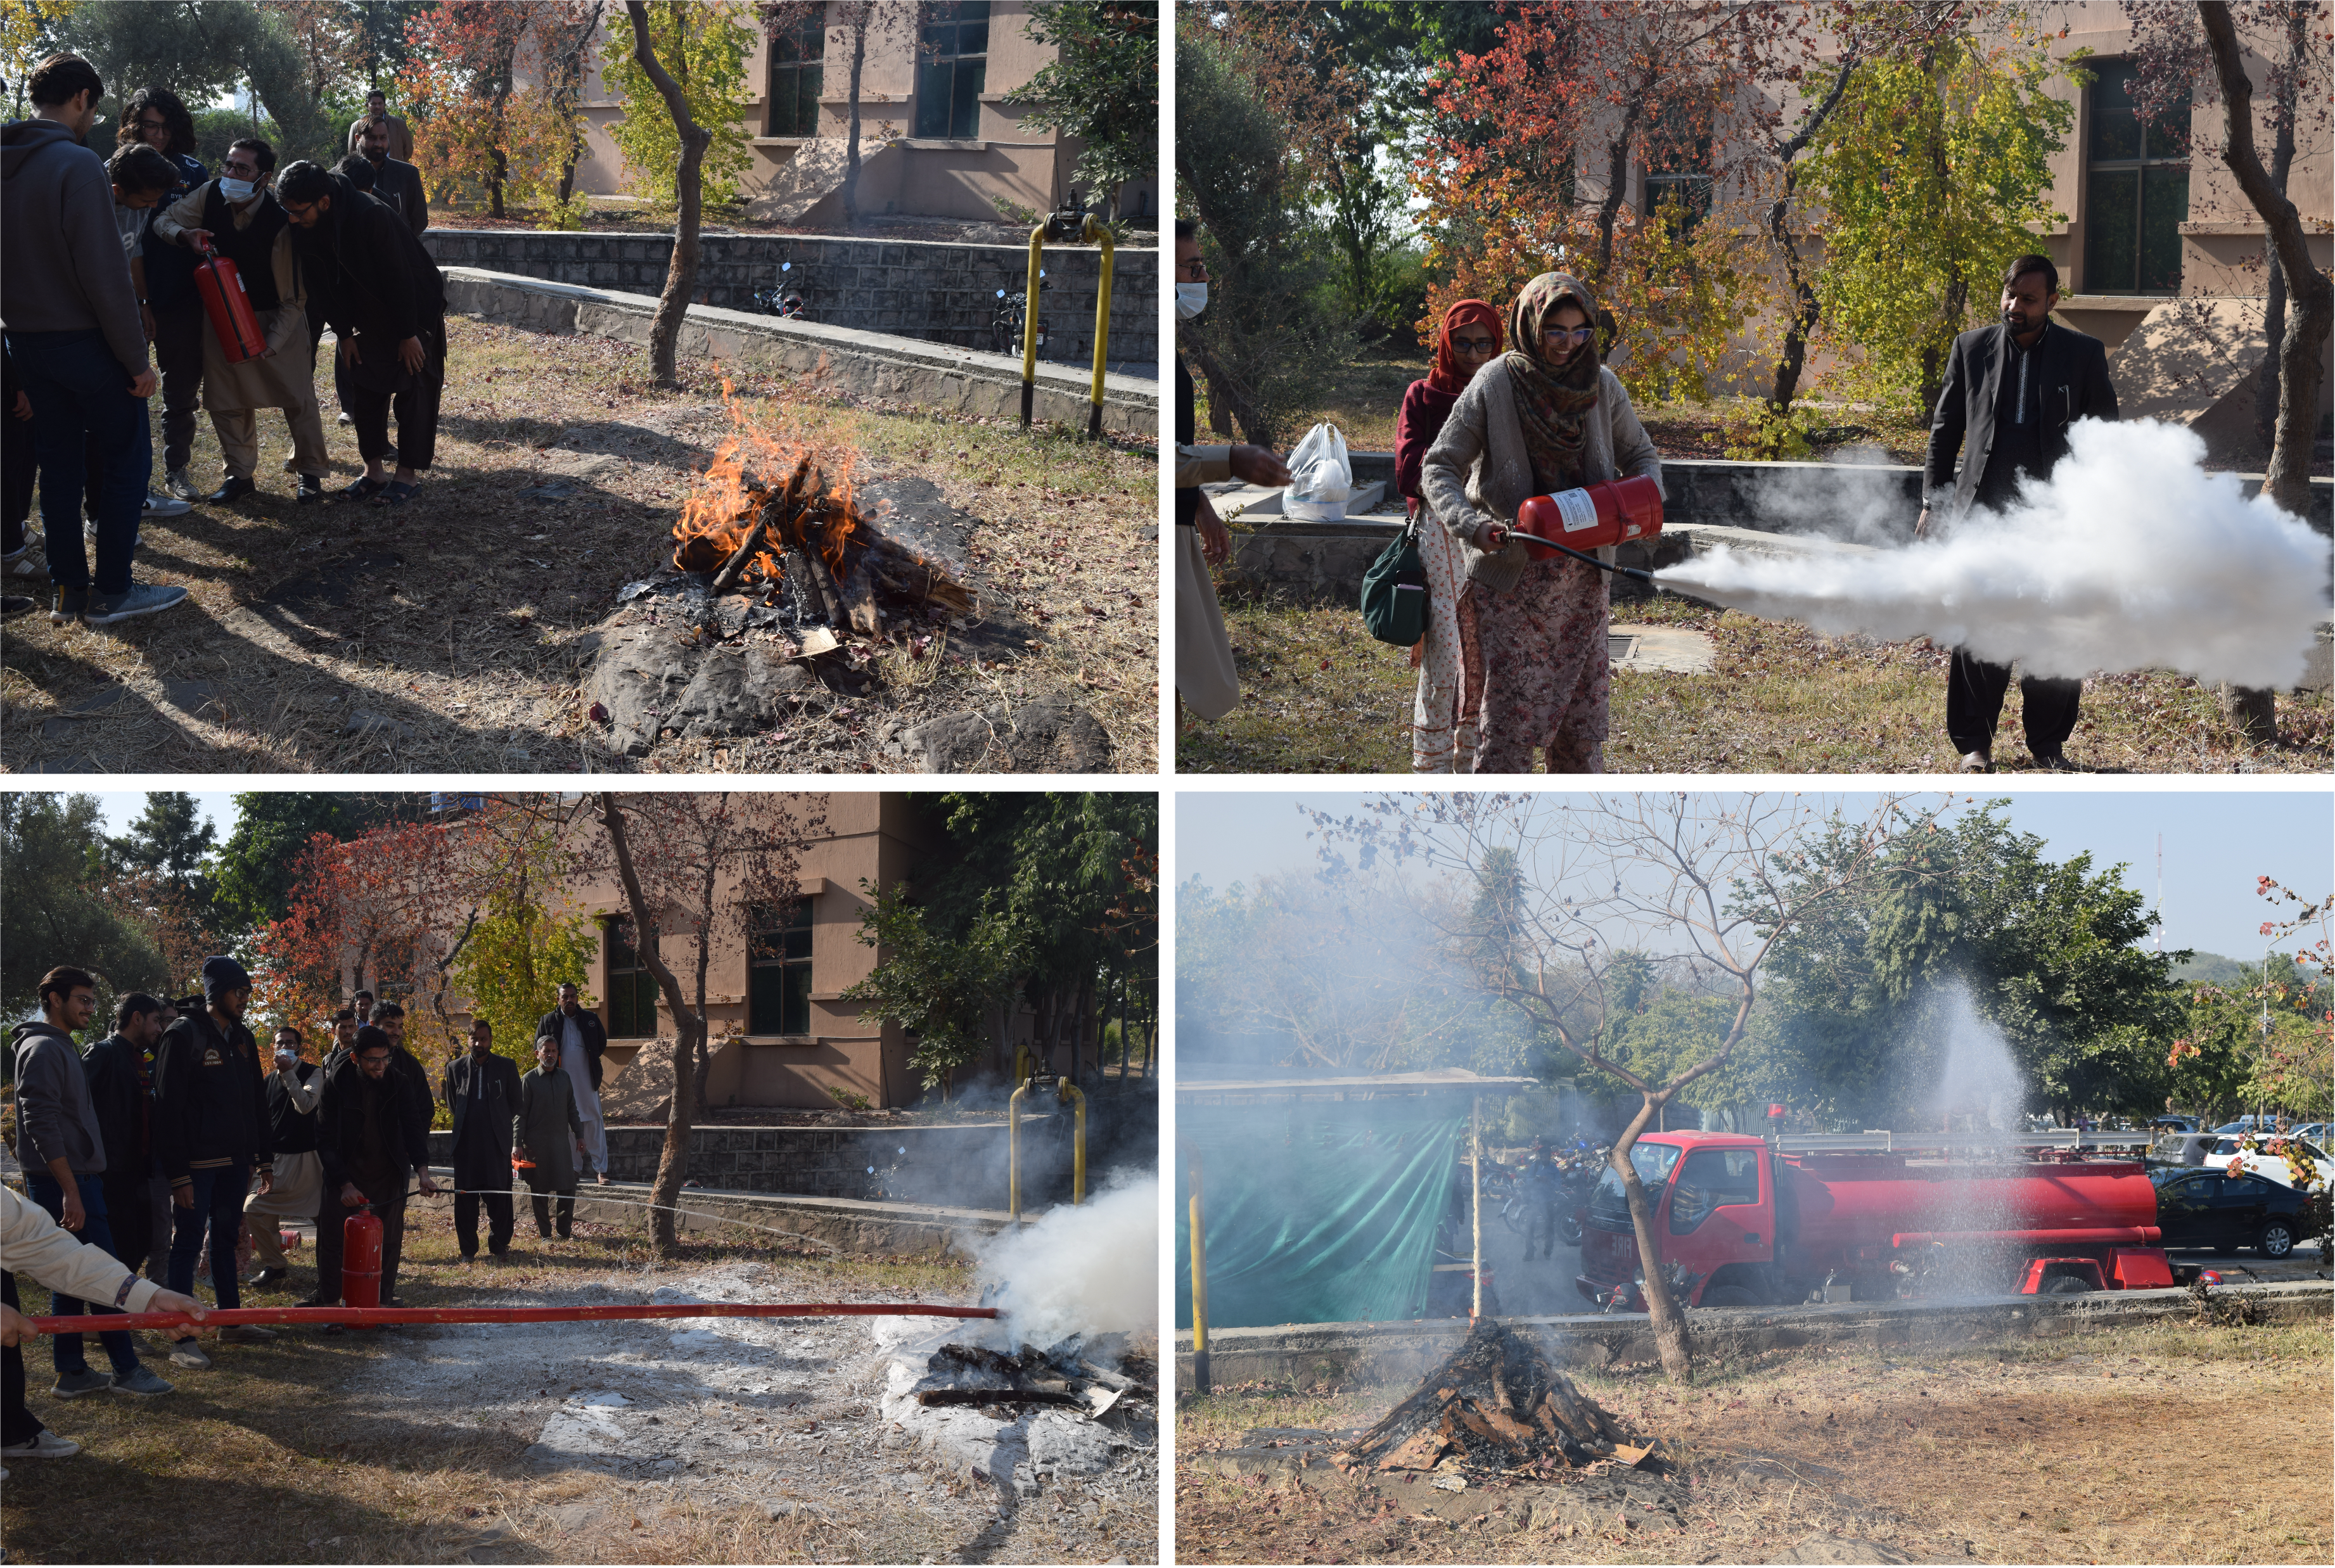
\includegraphics[width=1.0\textwidth]{images/criterion_6/media/img7.png}
    \caption{Fire drill exercise conducted at SEECS for awareness and preparedness of students and staff.}
    \label{fire_drill}
\end{figure}
\clearpage

% ============================================================
% CHAPTER 8 — Criterion 7: Institutional Support and Financial Resources
% Images: images/criterion_7/media/
% ============================================================
\graphicspath{{images/criterion_7/media/}}
\hypertarget{criterion-7-institutional-support-and-financial-resources}{%
\chapter{Criterion 7: Institutional Support and Financial Resources}\label{criterion-7-institutional-support-and-financial-resources}}

\hypertarget{financial-governance-sustainability-c7}{%
\section{Financial Governance and Sustainability}\label{financial-governance-sustainability-c7}}

NUST manages financial resources through a centralized budgeting and monitoring framework involving academic departments, schools, and central administration. Annual allocations are based on academic requirements, enrolment, infrastructure needs, and research priorities. Recurring expenditure supports salaries, laboratory operations, maintenance, software and other routine requirements, while developmental expenditure supports laboratory equipment, computing infrastructure and facility enhancement. Budget utilization, procurement and audit are governed through established University procedures and applicable public procurement regulations.

SEECS demonstrates sustained financial capacity throughout the accreditation cycle. Table~\ref{tab:c7_financial_trends} summarizes the principal financial indicators; detailed account-head-wise budgeted and actual figures are provided in Annexure~\ref{annex:L}.

\begin{table}[H]
\centering
\caption{Key Financial Indicators, SEECS (Rupees in Million, Actual)}
\label{tab:c7_financial_trends}
\begingroup\footnotesize
\setlength{\tabcolsep}{4.5pt}
\renewcommand{\arraystretch}{1.12}
\begin{tabular}{@{}lrrrr@{}}
\toprule
\textbf{Indicator} & \textbf{2022--23} & \textbf{2023--24} & \textbf{2024--25} & \textbf{2025--26} \\
\midrule
Recurring expenditure & 486.408 & 508.979 & 622.386 & 731.382 \\
Development expenditure & 14.700 & 15.100 & 81.950 & 74.820 \\
Research project funding & 46.583 & 70.217 & 73.262 & 69.940 \\
Student tuition fee (self-funded) & 594.764 & 753.222 & 889.700 & 1107.514 \\
Scholarship support & 27.797 & 17.788 & 14.344 & 12.527 \\
\bottomrule
\end{tabular}
\endgroup
\end{table}

Recurring expenditure increased from Rs.~486.408~M in 2022--23 to Rs.~731.382~M in 2025--26, while developmental expenditure rose substantially in 2024--25 and 2025--26 due primarily to laboratory and infrastructure investment. In parallel, internally generated tuition income and externally funded research provide complementary revenue streams. These trends demonstrate continued institutional commitment and sufficient financial capacity to sustain the Software Engineering program.

\hypertarget{human-resource-academic-support-c7}{%
\section{Human Resource and Academic Support}\label{human-resource-academic-support-c7}}

A major component of recurring expenditure is the provision of qualified faculty and support staff. Actual expenditure on faculty and support-staff salaries increased from Rs.~461.508~M in 2022--23 to Rs.~632.311~M in 2025--26. NUST additionally supports employee benefits, faculty development, higher education, research incentives, conference participation and professional training. Faculty recruitment, qualifications, workload and current strength are reported in Criterion 5; duplicating these figures here is avoided to maintain a single authoritative record.

Academic delivery is further supported through centralized student services, information technology, learning-management systems, library and digital resources, and administrative support. These resources are funded through the University's recurring and developmental mechanisms and are available to the Software Engineering program as part of the broader SEECS/NUST institutional infrastructure.

\hypertarget{infrastructure-laboratory-support-c7}{%
\section{Infrastructure and Laboratory Support}\label{infrastructure-laboratory-support-c7}}

Institutional investment during the accreditation cycle has focused strongly on laboratory modernization, computing facilities and upkeep of existing infrastructure. The four-year actual expenditure shown in Table~\ref{tab:c7_lab_support} is derived from the detailed financial record in Annexure~\ref{annex:L}.

\begin{table}[H]
\centering
\caption{Four-Year Laboratory and Facility Support, SEECS (Rupees in Million, Actual)}
\label{tab:c7_lab_support}
\begingroup\footnotesize
\setlength{\tabcolsep}{8pt}
\renewcommand{\arraystretch}{1.12}
\begin{tabular}{@{}lr@{}}
\toprule
\textbf{Support Area} & \textbf{2022--23 to 2025--26} \\
\midrule
Laboratory equipment & 164.770 \\
Software purchase & 21.800 \\
Laboratory consumables & 3.000 \\
Maintenance of existing facilities & 153.888 \\
Repair and maintenance & 4.640 \\
\midrule
\textbf{Total} & \textbf{348.098} \\
\bottomrule
\end{tabular}
\endgroup
\end{table}

The increase in laboratory-equipment expenditure to Rs.~71.55~M in 2024--25 and Rs.~74.82~M in 2025--26 provides direct evidence of continued investment in modernization. Computing laboratories, networking, licensed software and associated facilities used by the program are described in detail under Criterion 6; the financial evidence here demonstrates the institutional capacity to establish, operate, maintain and upgrade those facilities.

\hypertarget{research-innovation-student-support-c7}{%
\section{Research, Innovation and Student Support}\label{research-innovation-student-support-c7}}

NUST supports research and innovation through institutional facilitation and externally sponsored projects. SEECS received approximately Rs.~260.0~M in research project funding over the four-year accreditation cycle, with annual funding remaining between Rs.~69.9~M and Rs.~73.3~M during the most recent three years. Faculty and students are supported through research infrastructure, project activities, consultancy and industry collaboration, prototype development, scholarly dissemination and participation in innovation activities.

Student financial support is provided through Board, GPA-based, HEC, MS-leading-to-PhD and need-based scholarship schemes. Cumulative scholarship support during 2022--23 to 2025--26 was approximately Rs.~72.46~M. Scheme-wise annual figures are retained in Annexure~\ref{annex:L} as primary evidence.

\hypertarget{criterion7-compliance-summary}{%
\section{Criterion 7 Compliance Summary}\label{criterion7-compliance-summary}}

\begin{table}[H]
\centering
\caption{Evidence Summary for PEC Criterion 7}
\label{tab:c7_evidence_summary}
\begingroup\footnotesize
\setlength{\tabcolsep}{7pt}
\renewcommand{\arraystretch}{1.08}
\begin{tabular}{@{}p{0.38\textwidth}p{0.50\textwidth}@{}}
\toprule
\textbf{Requirement} & \textbf{Primary Evidence} \\
\midrule
Financial sustainability & Table~\ref{tab:c7_financial_trends}; Annex~\ref{annex:L} \\
Continued financial commitment & Tables~\ref{tab:c7_financial_trends}--\ref{tab:c7_lab_support}; Annex L; Criterion 6 \\
Human-resource support & Salary expenditure; Criterion 5 faculty record \\
Research and innovation support & Research funding in Table~\ref{tab:c7_financial_trends}; project records \\
Student financial support & Scholarship expenditure; Annex~\ref{annex:L} \\
\bottomrule
\end{tabular}
\endgroup
\end{table}

The financial and institutional evidence demonstrates sustained support for academic operations, human resources, laboratories, research and students throughout the accreditation cycle. The upward trend in recurring expenditure, major developmental investment in the two most recent years, continued research funding and documented student support collectively establish that the Software Engineering program has adequate and sustainable institutional resources to meet the requirements of PEC Criterion~7.

\clearpage

% ============================================================
% CHAPTER 9 — Criterion 8: Continual Quality Improvement
% Images: images/criterion_8/media/
% ============================================================
\graphicspath{{images/criterion_8/media/}}
\hypertarget{criterion-8-continual-quality-improvement}{%
\chapter{Criterion 8: Continuous Quality Improvement (CQI)}\label{criterion-8-continual-quality-improvement}}

\hypertarget{sec:9.1general-nust-quality-enhancement-cell}{%
\section{General -- NUST Quality Enhancement Cell}\label{general-nust-quality-enhancement-cell}}

Lately, the realization of the need for quality assurance in higher education has become a global phenomenon. NUST also felt the need to assess and improve the quality of higher education in the country, with the objective of achieving international competitiveness and compatibility of its academic programs and research quality. Considering this NUST Quality Assurance Directorate takes care of quality assurance policies in all institutions of NUST. Organizational structure of NUST Quality Assurance (QA) Directorate is illustrated in Figure~\ref{fig:sample}.
\begin{figure}[h]
    \centering
    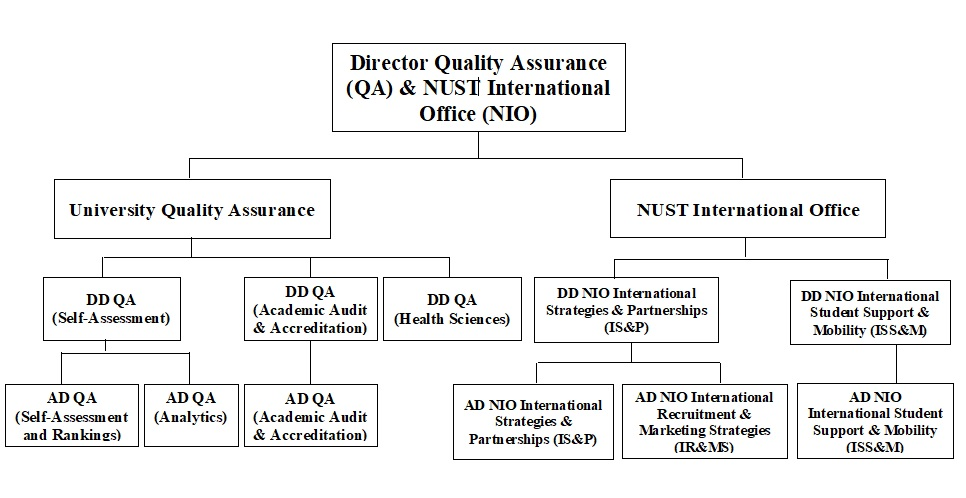
\includegraphics[width=0.8\textwidth]{images/criterion_8/media/nustqa.jpg}
    \caption{Organizational structure of NUST Quality Assurance Directorate}
    \label{fig:sample}
\end{figure}


One of the tasks of NUST QA is the academic quality audit of all the programs at NUST that carried out annually or periodically as deemed necessary, to ensure quality of program and identify any flaw and drawbacks in the program. The NUST Quality Assurance Directorate is committed to ensuring excellence in education and research by implementing a comprehensive quality assurance framework aligned with national and international standards. Its vision is to deliver high-quality education that is globally competitive, while its mission focuses on developing and implementing quality assurance policies, building faculty and staff capacity, conducting systematic assessments and audits, enhancing academic quality, and promoting internationalization. The Directorate's objectives include implementing the Higher Education Commission's quality assurance framework, conducting self-assessment and internal quality audits, ensuring compliance with accreditation requirements, improving teaching, research, and support services, strengthening institutional capacity, supporting university rankings through data management, fostering national and international collaborations, and contributing to quality enhancement in higher education. Established in 2005 as one of the first Quality Enhancement Cells under the HEC initiative, the QA directorate adopts a holistic, continuous quality improvement approach centered on self-assessment, evidence-based evaluation, and institutional excellence.


\hypertarget{local-quality-enhancement-cell-lqec}{%
\section{Local Quality Enhancement Cell (LQEC)}\label{local-quality-enhancement-cell-lqec}}

To ensure the effective implementation of Continuous Quality Improvement (CQI), the Department has designated the Director Local Quality Enhancement Cell (DLQEC) as the focal person for coordinating quality assurance and continuous improvement activities. The CQI Committee, headed by the Head of Department (HoD), provides oversight of the CQI process by reviewing assessment and feedback data, evaluating the corrective actions proposed by the DLQEC, recommending additional improvement measures where required, and monitoring the implementation and effectiveness of the approved actions. Through this process, the committee ensures that quality enhancement initiatives are systematically implemented and continuously monitored across the program. The structure of the CQI Committee is shown in Figure~\ref{fig:sample1}.
\begin{figure}[h]
    \centering
    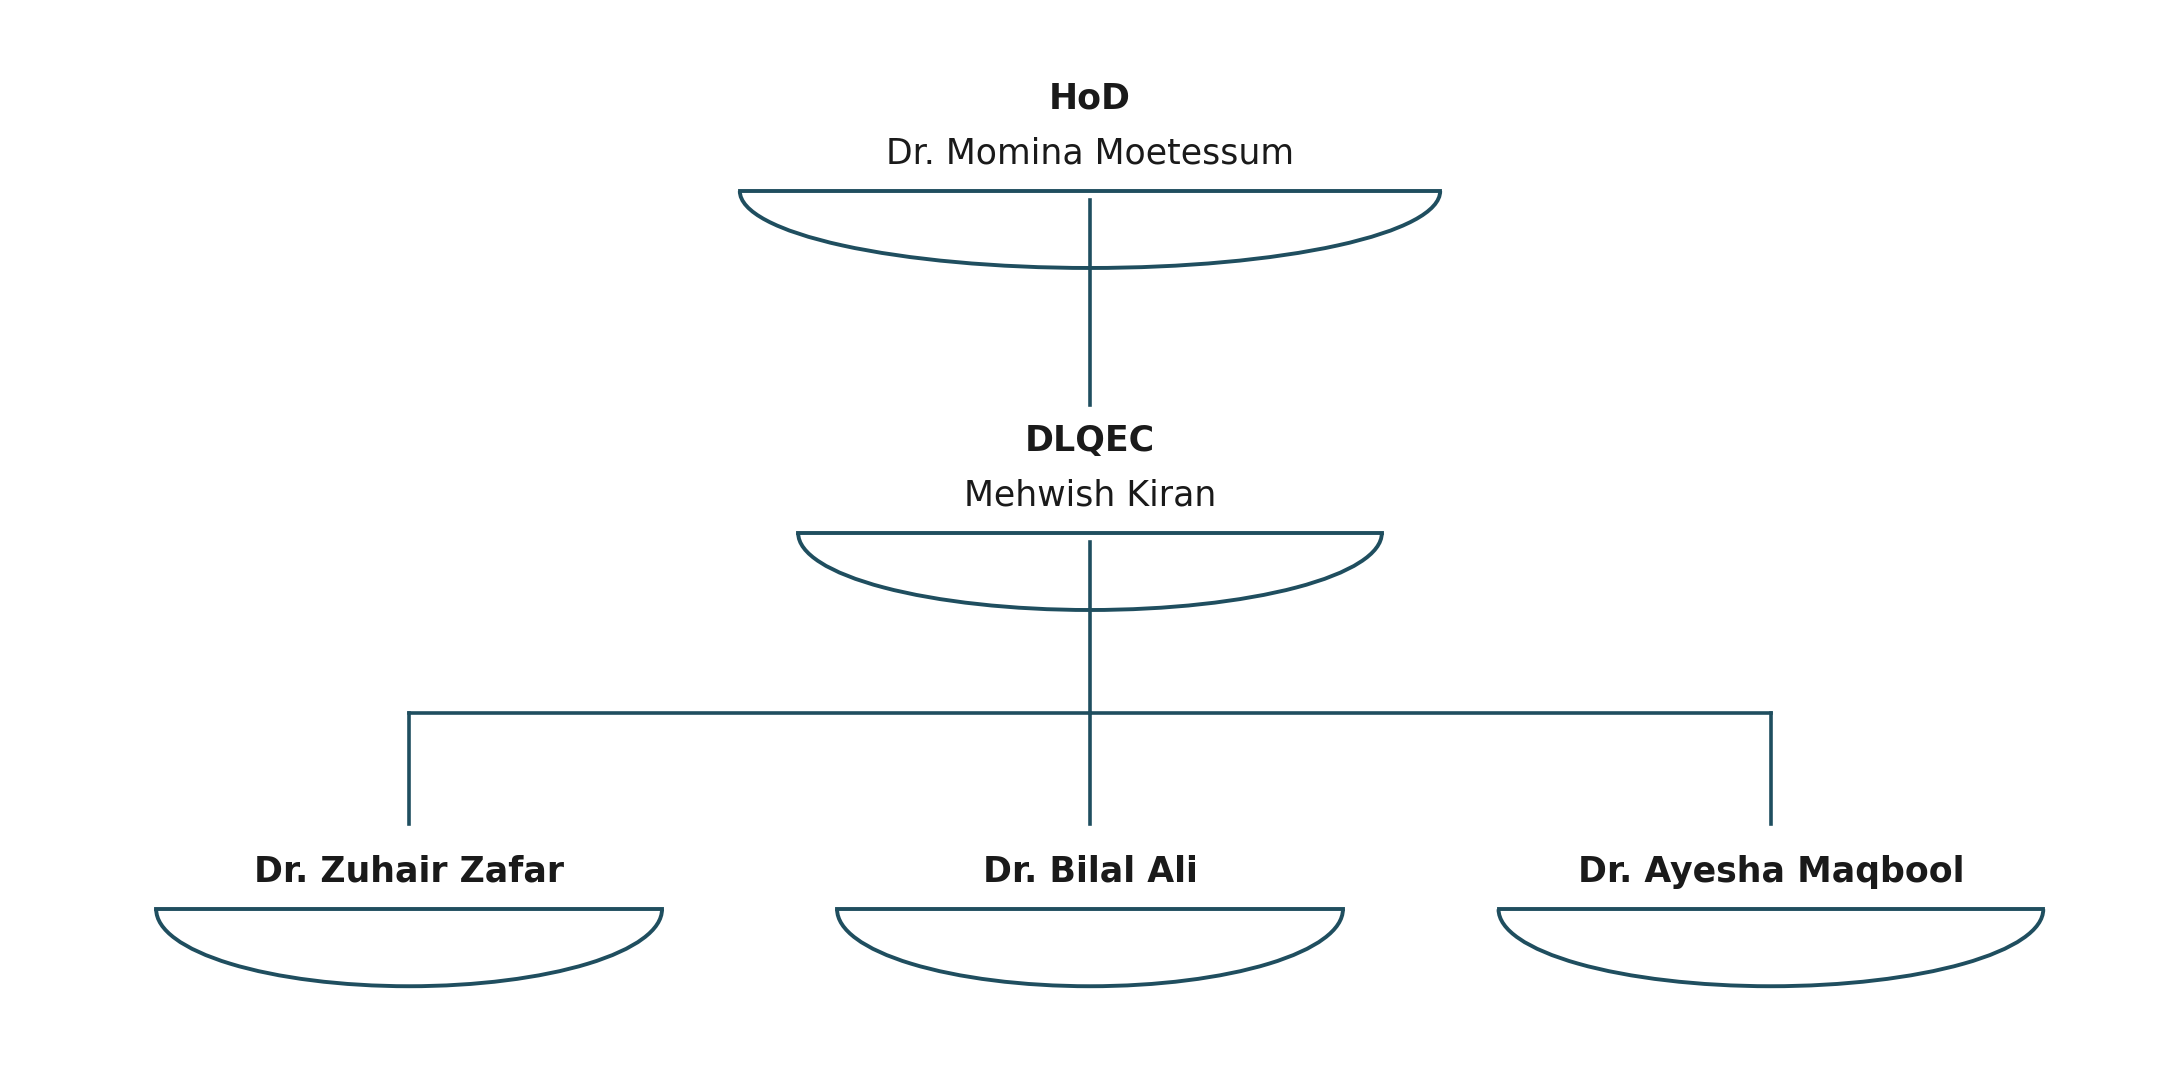
\includegraphics[width=0.8\textwidth]{images/criterion_8/media/Figure_9.2_CQI_Committee_Structure.png}
    \caption{CQI Committee Structure}
    \label{fig:sample1}
\end{figure}

For program accreditation, the DLQEC coordinates the preparation of the SAR and supports SEECS in all activities related to accreditation readiness. The DLQEC also assists in organizing the required documentation, coordinating with relevant stakeholders, and facilitating the Institute's preparations for the accreditation visit and presentations to the members of the accreditation team. The observations made during the accreditation visits are also scrutinized by CQI Committee and is responsible for implementation of any points or concerns raised during the visit. Last PEC visit was carried out in October/November 2023 and the observations with their replies are given in (Rejoinder) Annexure~\ref{annex:rejoinder}.

\hypertarget{program planning}{%
\section{Program Planning}\label{Program Planning}}
Program planning is conducted through a structured and collaborative process to ensure the effective delivery of academic, laboratory, and co-curricular activities throughout the academic year. 
At the beginning of each academic year, an annual academic plan is developed in alignment with the university's academic calendar, outlining key activities such as semester commencement, examinations, curriculum review meetings,  accreditation-related tasks, faculty development programs, industrial visits, seminars, and CQI activities. Sample for academic calendar is shown at Annexure~\ref{annex:planner}.

Prior to the commencement of each semester, detailed semester planning is carried out, including the finalization of course offerings, class schedules, examination timelines, and student advising activities. Resource planning is undertaken to ensure the availability of classrooms, laboratories, software licenses, computing facilities, and other teaching resources required for the smooth execution of academic activities by Academic Coordination Branch (ACB) and IT department.

Faculty allocation is performed based on faculty expertise, teaching workload, specialization, and previous teaching experience to ensure effective course delivery while maintaining a balanced distribution of responsibilities. Laboratory planning includes the review of laboratory manuals, preparation of equipment, software installation, procurement of consumables, scheduling of laboratory sessions, and assignment of laboratory instructors to support practical learning outcomes.

Final Year Design Project planning is initiated well before the start of the academic session through the identification of research domains, allocation of supervisors according to expertise, proposal evaluation, milestone scheduling, progress monitoring, and final project evaluations. The overall planning process is regularly reviewed through departmental meetings and feedback mechanisms, enabling timely adjustments and ensuring continuous improvement in academic quality and program effectiveness.

\hypertarget{cqi-process-in-obe-implementation}{%
\section{CQI Process in OBE Implementation}\label{cqi-process-in-obe-implementation}}

The Department of Software Engineering has established a comprehensive Continuous Quality Improvement framework to ensure the continuous enhancement of its curriculum and Outcome-Based Education implementation. The framework comprises four interconnected CQI processes covering the curriculum, CLOs, PLOs, and PEOs. The CQI model is shown in Figure~\ref{fig:sample2}. Each process follows a systematic cycle of data collection, evaluation, review, and implementation of corrective actions, ensuring that assessment results are effectively utilized to improve academic quality and maintain compliance with HEC and PEC requirements.
\begin{figure}[h]
    \centering
    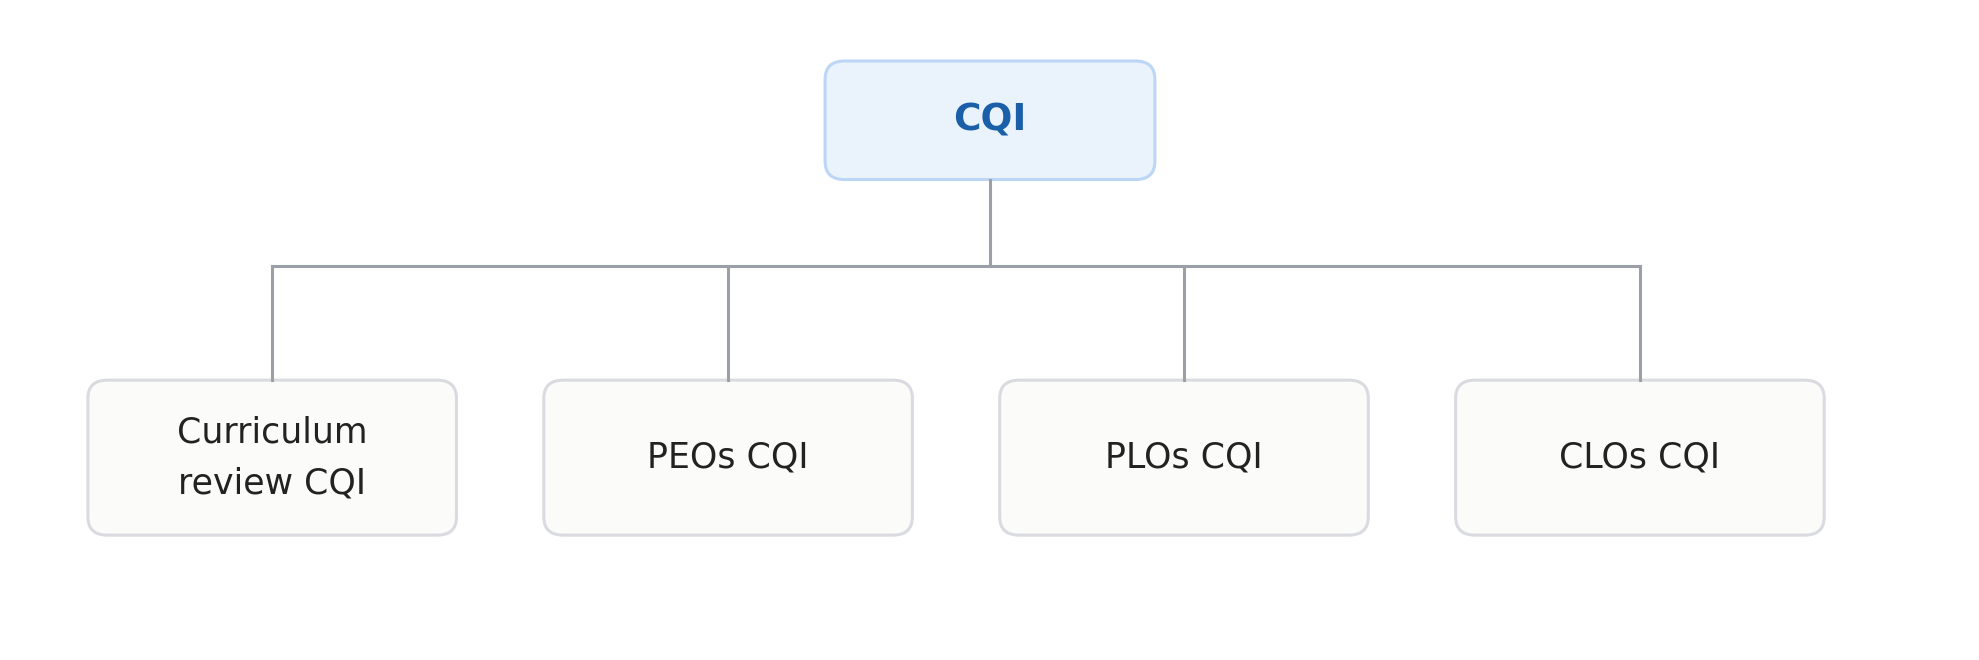
\includegraphics[width=0.8\textwidth]{images/criterion_8/media/cqi_flow.png}
    \caption{CQI Model of Software Engineering Department}
    \label{fig:sample2}
\end{figure}


To ensure that the curriculum remains relevant, effective, and aligned with evolving academic standards, technological advancements, industry requirements, and stakeholder expectations, the department follows a structured Curriculum CQI process. The process involves systematic collection and analysis of feedback from key stakeholders, review of academic performance and assessment outcomes, and consideration of regulatory and accreditation requirements. Based on this analysis, recommendations for improvement are formulated, reviewed through the appropriate academic forums, and implemented in subsequent curriculum revisions, thereby ensuring the continuous enhancement of the program.

The CQI process for CLOs, PLOs, and PEOs is illustrated in Figure~\ref{fig:sample3} through three interconnected loops. 
\begin{figure}[h]
    \centering
    \includegraphics[width=0.8\textwidth]{images/criterion_8/media/peo-evaluation.png}
    \caption{CQI Process for CLOs, PLOs and PEOs}
    \label{fig:sample3}
\end{figure}
The innermost loop focuses on CLO attainment, which is evaluated at the end of each semester using direct assessment methods. The results are documented in Course Review Reports and corrective actions related to teaching strategies, assessment methods, or course content are implemented where required. CLO attainment forms the primary evidence for the direct assessment of PLOs, while indirect evidence is obtained through graduate exit survey and internship feedback forms. PLO attainment is reviewed after every semester to identify improvement opportunities in curriculum, teaching, and assessment practices. The outermost loop evaluates the achievement of PEOs using indirect assessment method which includes feedback from alumni and employers, typically four years after graduation. The collected data is analyzed and evaluated, and if required, corrective actions are initiated through a corrective action form as shown at Annexure~\ref{annex:corrective}. CQI for curriculum and the OBE implementation model for PEOs, PLOs and CLOs are described separately in the following paragraphs.
\hypertarget{criterion-8-Curriculum }{%
\section{Curriculum}\label{criterion-8-curriculum}}

The Department has established a systematic and evidence-based curriculum review mechanism as part of its CQI framework. The mechanism ensures that the curriculum remains current, relevant, and aligned with the requirements of the PEC, HEC, emerging technological developments, and the expectations of academia and industry. Curriculum improvements are driven through periodic evaluation of assessment data and structured stakeholder feedback, and are implemented following the University's prescribed approval process.
\hypertarget{criterion-8-CQI Process for Curriculum}{%
\subsection{CQI Process for Curriculum}\label{cqi-process-for-curriculum}}
Figure~\ref{fig:sample4} illustrates the Curriculum CQI process followed by the Department to ensure that the curriculum remains current, outcome-based, and aligned with the requirements of HEC, PEC, industry, and other stakeholders. The process begins with the collection of curriculum and course-related data from the departmental database, together with feedback from students, faculty, alumni, employers, the Industrial Advisory Board (IAB), and regulatory bodies. These inputs are reviewed by the DLQEC and subsequently evaluated by the HOD and Departmental Board of Studies (DBS), where recommendations for curriculum improvement are formulated. Proposed revisions are then processed through the university's approval hierarchy. Changes involving up to 10\% of the curriculum are approved by the Faculty Board of Studies (FBS), while revisions involving more than 10\% and up to 50\% require approval from the University Curriculum Review Committee (UCRC). Major curriculum revisions involving more than 50\% of the curriculum are submitted to the Academic Council (AC) for approval. Once the required approvals are obtained, the revised curriculum is implemented and updated in the departmental database, thereby completing the CQI cycle and ensuring the continuous improvement of the academic program.

\begin{figure}[h]
    \centering
    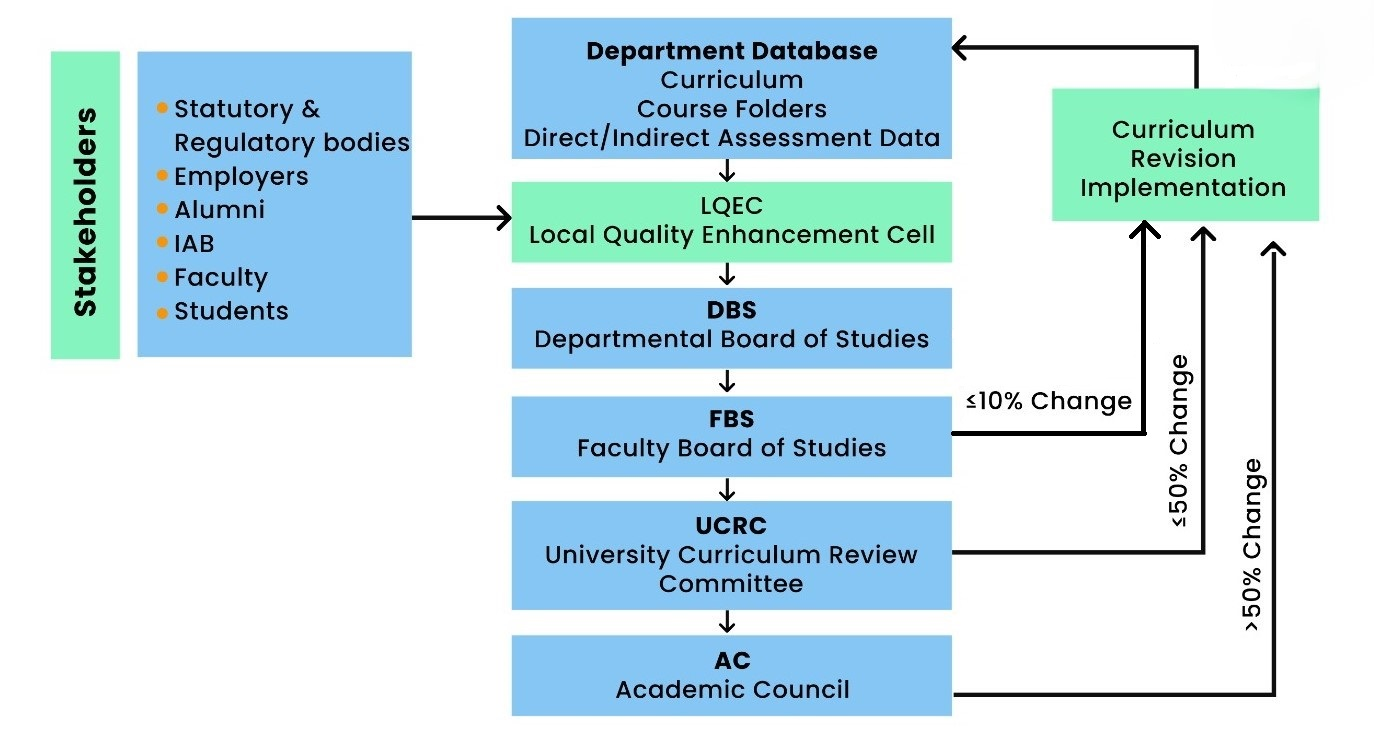
\includegraphics[width=0.8\textwidth]{images/criterion_8/media/Curr_review.jpeg}
    \caption{Curriculum Review Process}
    \label{fig:sample4}
\end{figure}

\hypertarget{criterion-8-Corrective Actions for Curriculum}{%
\subsection{Corrective Actions for Curriculum}\label{criterion-8-corrective-actions-for-curriculum}}

Table~\ref{tab:cqi_actions1} shows few corrective actions taken to improve the curriculum
\begin{table}[ht]
\centering
\footnotesize
\setlength{\tabcolsep}{4pt}

\begin{tabular}{
>{\raggedright\arraybackslash}p{4cm}
>{\raggedright\arraybackslash}p{2cm}
>{\raggedright\arraybackslash}p{3cm}
>{\raggedright\arraybackslash}p{2.8cm}
>{\raggedright\arraybackslash}p{3cm}
}
\toprule
\textbf{Observation} &
\textbf{Source} &
\textbf{Decision} &
\textbf{Action Taken} &
\textbf{Evidence} \\
\midrule
Need more software engineering electives &
IAB \& PEC  &
Added extra elective &
Updated Curriculum &
Working Paper in Annexure~\ref{annex:wp2025} \\

Inclusion of New Courses &
PEC and HEC &
Inclusion of Fehm-ul-Quran \& Pak Studies &
Updated Curriculum &
Working Paper Annexure~\ref{annex:wp2024}  \& ~\ref{annex:wp2025}  \\

Faculty Load &
HnS Faculty &
Swap Courses across semester &
Updated Scheme &
Curriculum \\

Topic Addition in Course Outline &
IAB &
Inclusion of the new topics &
Added "Rest API" in Web Engineering.  &
Course Outline \\
\bottomrule
\end{tabular}
\caption{Examples of CQI Actions}
\label{tab:cqi_actions1}
\end{table}

\hypertarget{criterion-8-peos}{%
\section{PEOs}\label{criterion-8-peos}}

\hypertarget{criterion-8-cqi-process-for-peos}{%
\subsection{CQI Process for PEOs}\label{criterion-8-cqi-process-for-peos}}

The DLQEC is responsible for the initiation of CQI for attainment, revision, and improvement of PEOs. CQI committee reviews the corrective actions to meet the desired criteria. The process of CQI for PEOs is shown in Figure~\ref{fig:sample5}. PEOs are indirectly assessed through alumni and employer surveys, where the data is collected yearly, with evaluation and review carried out four years after graduation of each batch. 

\begin{figure}[h]
    \centering
    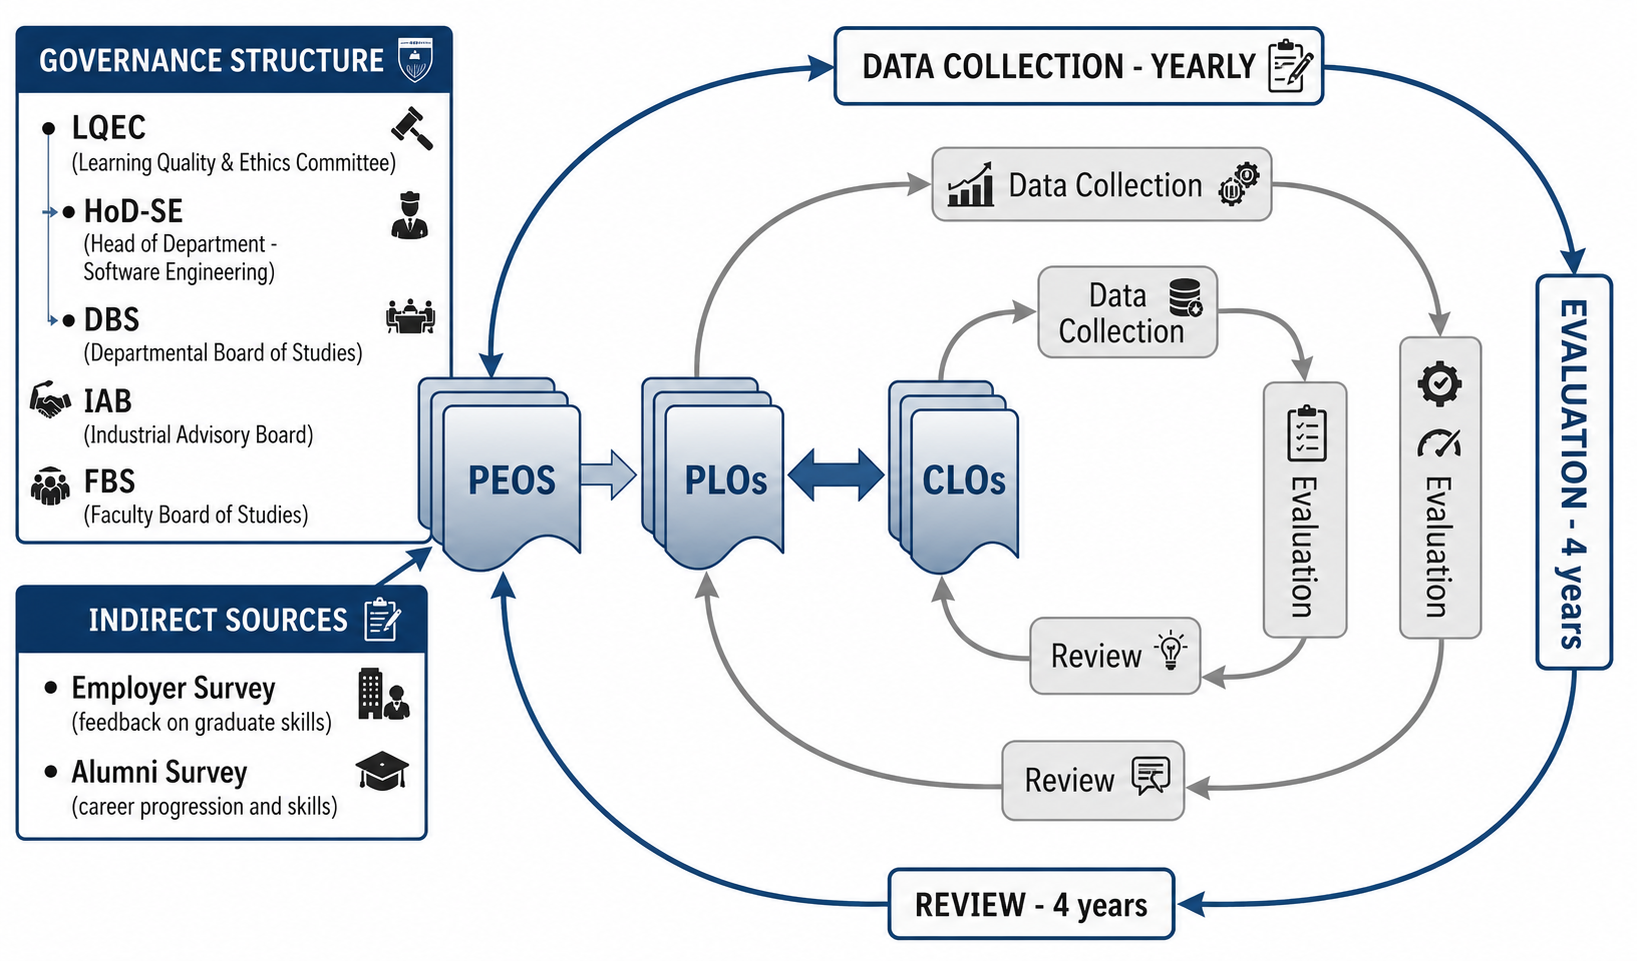
\includegraphics[width=0.8\textwidth]{images/front_matter/media/image13.png}
    \caption{CQI Process for PEOs}
    \label{fig:sample5}
\end{figure}


\hypertarget{criterion-8-review-processe-for-peos}{%
\subsection{Review Process for PEOs}\label{criterion-8-review-processe-for-peos}}

The review process starts with the measurement of PEOs and involves CQI, corrective actions, and administrative processes for the maintenance and/or improvement of PEO as shown in Figure~\ref{fig:sample6}. If the achievement of PEO is achieved, no corrective action is required; otherwise, DLQEC.invokes the CQI process. The CQI process leads to one or more corrective actions namely, revision of PEOs, revision of KPIs for PEOs, revision of assessment methods, and/or revision of curriculum/strategies. Any corrective actions if required are initiated by DLQEC and reviewed by CQI committee and may progressively be taken up to AC as mentioned previously in Criteria 1.

\begin{figure}[ht]
\centering
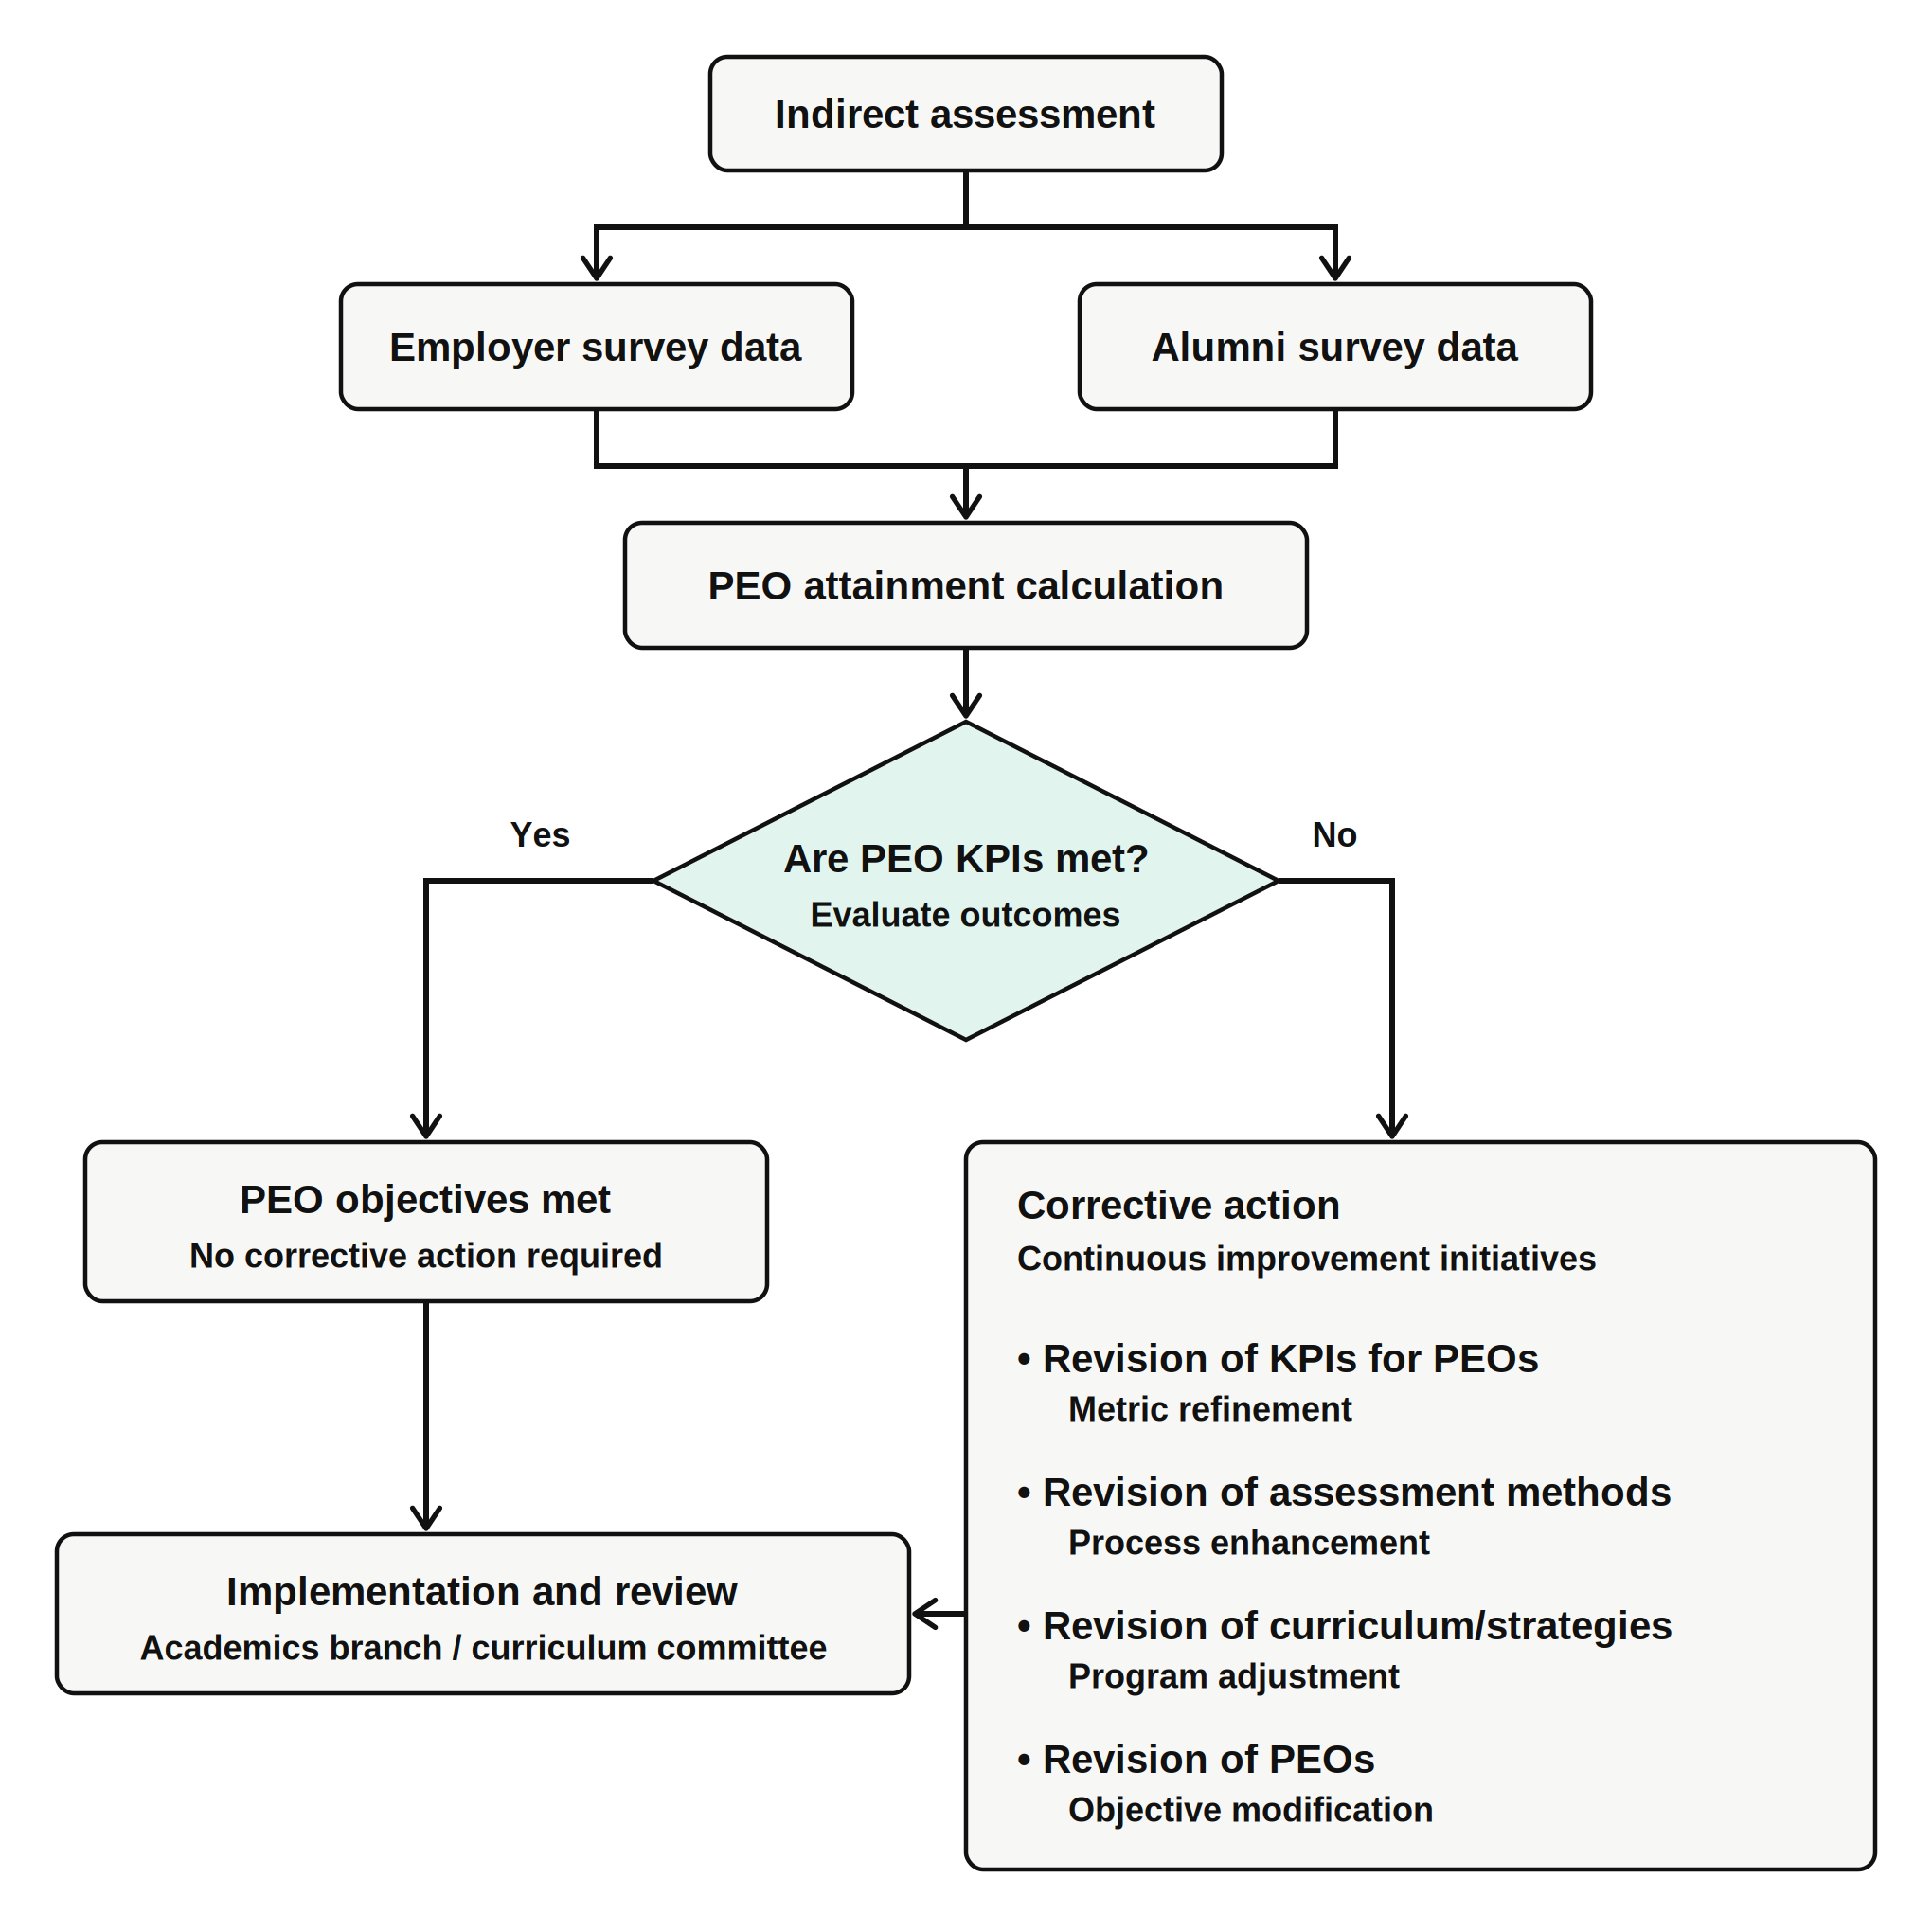
\includegraphics[width=0.89\textwidth]{images/front_matter/media/image-14.png}
\caption{Flowchart Showing Review \& Corrective Action Processes for PEOs}
\label{fig:sample6}
\end{figure}

\hypertarget{criterion-8-corrective-actions-for-peos}{%
\subsection{Corrective Actions for PEOs}\label{criterion-8-corrective-actions-for-peos}}

Figure~\ref{fig:sample7} presents the attainment of each KPI for the PEOs under the legacy evaluation system for data collected in 2025. The dashed line in each graph represents the required attainment threshold (50\% or 60\%, depending on the KPI). The result show that all KPI achieved their respective thresholds, except PEO-1, KPI-6 (pursuing higher education), which did not meet the required 50\% attainment threshold.

\begin{figure}
    \centering
    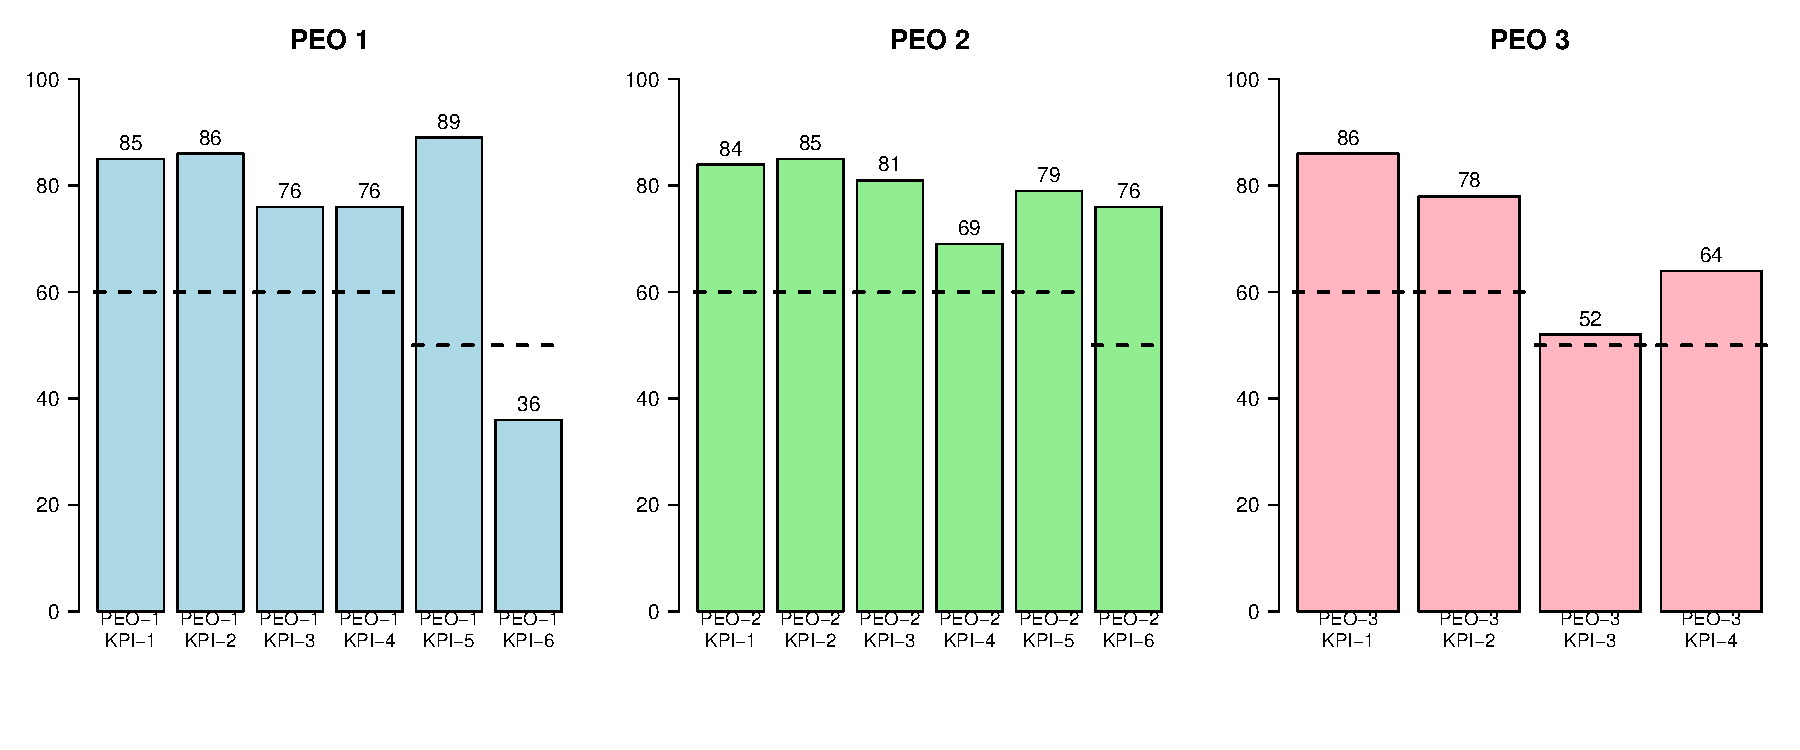
\includegraphics[width=0.8\textwidth]{images/criterion_1/media/legacy_analysis.pdf}
    \caption{Per-KPI attainment under the Legacy Evaluation System (data collected in 2025)}
    \label{fig:sample7}
\end{figure}

After analysis, the CQI committee concluded that the only KPI that did not meet the required threshold highlights a limitation of the legacy evaluation system rather than a weakness in the program. The indicator "pursuing higher education" is based on a simple yes/no outcome and does not fully reflect the achievement of the corresponding PEO. Graduates who choose to start their professional careers instead of pursuing higher studies should not be considered to have failed to achieve the goal. This limitation, along with the use of indicators that were not closely aligned with the PEOs and a rigid pass/fail evaluation approach, led to the development of the revised evaluation system described earlier.

As a result, the assessment tools to measure PEOs attainment i.e The Alumni Survey form and The Employer Survey forms were revised. Subsequently the KPIs were also revised. The revised survey forms are attached in Annexure~\ref{annex:alumni} and Annexure~\ref{annex:employer}.
\hypertarget{criterion-8-plos}{%
\section{PLOs}\label{criterion-8-plos}}

\hypertarget{criterion-8-cqi-process-for-plos}{%
\subsection{CQI Process for PLOs}\label{criterion-8-cqi-process-for-plos}}

DLQEC is responsible for CQI process for evaluation and attainment of PLOs with its designed loop shown in Figure~\ref{fig:cqi-plo} PLOs are directly assessed through CLOs and final year projects whereas indirect assessment is done through internship feedback and exit surveys. The data is collected, evaluated, and reviewed at the end of each academic semester. The entire process of review and corrective actions for the attainment of PLOs is explained in the following section.

\begin{figure}[H]
\centering
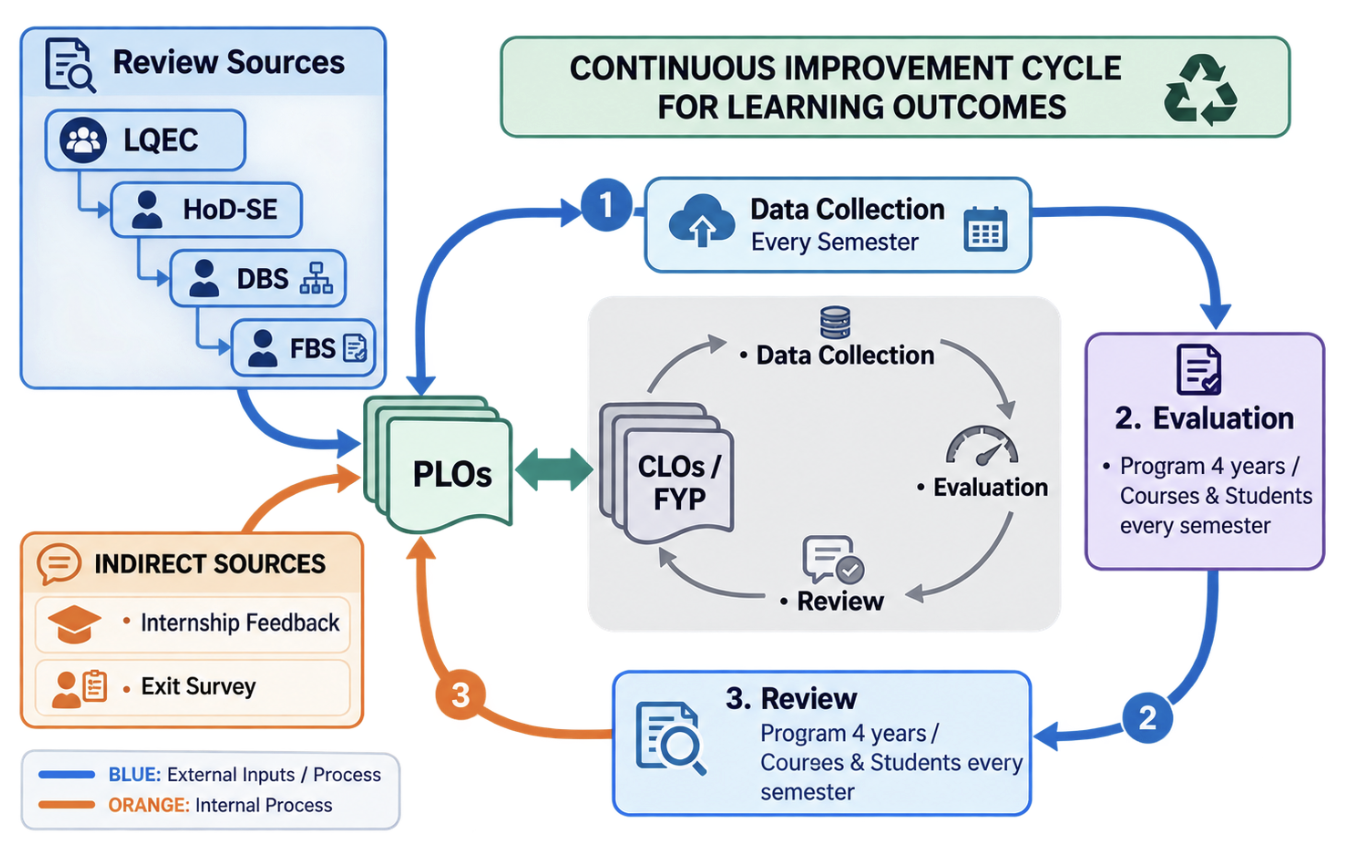
\includegraphics[width=0.88\textwidth]{images/front_matter/media/image-15.png}
\caption{CQI Process for PLOs}
\label{fig:cqi-plo}
\end{figure}

\hypertarget{criterion-8-review-process-for-plos}{%
\subsection{Review Process for PLOs}\label{criterion-8-review-process-for-plos}}


Figure~\ref{fig:individual-level} and Figure~\ref{fig:cohort-level} show the review process that starts with measurement of PLOs and involves corrective actions and administrative processes for maintenance and/or improvement of PLOs for individual as well as the cohort.  The attainment of PLOs is assessed from courses, final year design projects, internship feedback and exit surveys.  For individual students, if PLOs are attained, no corrective action is required as shown in Figure~\ref{fig:individual-level}. However, if an individual is not passing the PLOs different strategies are adopted for improvement. If an individual is not passing the PLOs in 4th – 6th semester, he/she will be counselled by the UG coordinator or student advisor, and a letter of advisory will be given to the student. If an individual does not pass PLO(s) in the 7th semester, a warning letter is issued to him. Lastly, if an individual does not pass PLO(s) in the 8th semester, a warning letter is handed to him and the department will give an extra module in the form of assignment, project study, case study, etc. to attain the deficient PLOs.


\begin{figure}[H]
\centering
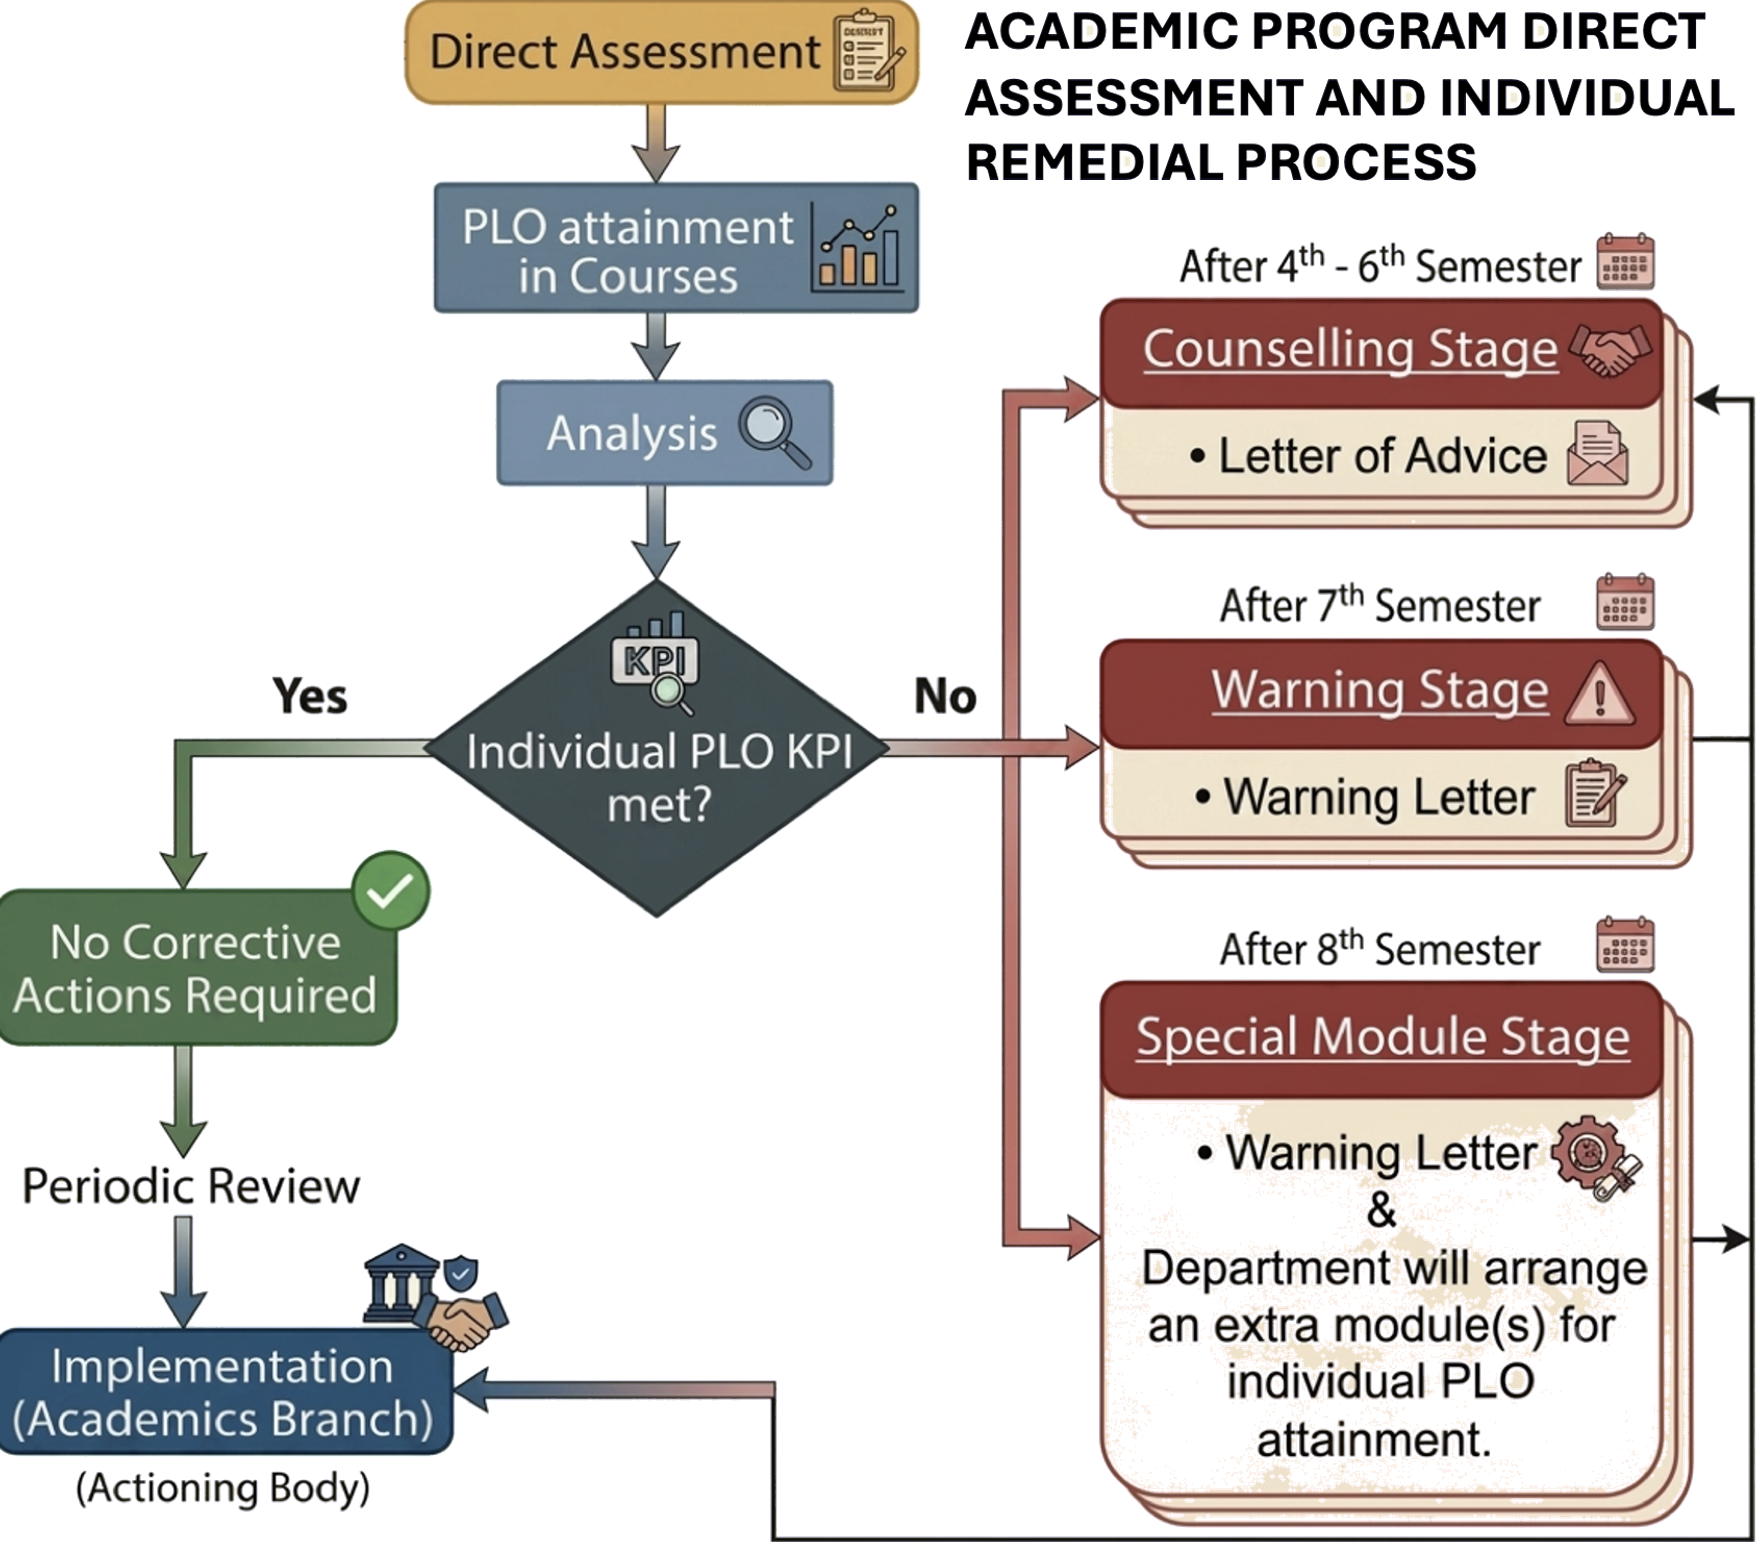
\includegraphics[width=0.7\textwidth]{images/front_matter/media/image-16.png}
\caption{Review of PLOs at Individual Level \& Corrective Actions}
\label{fig:individual-level}
\end{figure}

\begin{figure}[H]
\centering
\includegraphics[width=0.8\textwidth]{images/front_matter/media/image17.png}
\caption{Review of PLOs at Cohort Level \& Corrective Actions}
\label{fig:cohort-level}
\end{figure}

For cohort, if the PLOs attainment is more than or equal to 60 per cent as per KPI of each assessment, no corrective action is required.  However, if PLOs attainment is less than 60 per cent, the CQI process invokes corrective actions.  The CQI process leads to one or more corrective actions namely, revision of KPIs for PLOs, reassessment of courses related to PLOs, CLO-PLO remapping, curriculum revision, redefining / improvement of PLOs, review of teaching and learning processes, review of PLOs assessment methods, review of laboratory and equipment facilities, and review/ improvement of facilities and infrastructure as shown in Figure~\ref{fig:cohort-level}. Corrective actions if required are initiated by DLQEC, reviewed by CQI committee and may progressively be taken up to AC. 

\hypertarget{criterion-8-corrective-actions-for-plos}{%
\subsection{Corrective Actions for PLOs}\label{criterion-8-corrective-actions-for-plos}}

As evident from Figure~\ref{fig:sample8}, few students are failing PLO attainment at individual level. Advisory letters are sent to failing students and are continuously monitored. Sample of Letter of Advice sent to failing students is shared in Annexure~\ref{annex:advice}.
\begin{figure}[H]
    \centering
    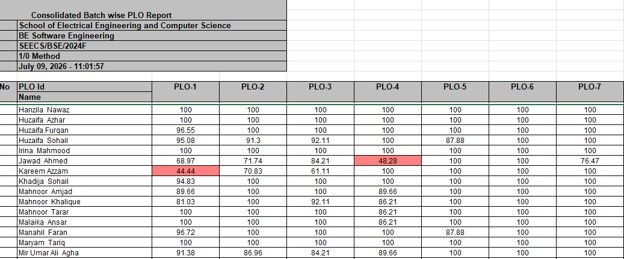
\includegraphics[width=0.8\textwidth]{images/criterion_8/media/PLO1.jpeg}
    \caption{Individual PLO Attainment for Batch2k24}
    \label{fig:sample8}
\end{figure}

The following reports show the Cohort Level Summary of PLO Attainment for Batch 2022 through CLOs, Exit Survey and Internship feedback survey respectively in Figures~\ref{fig:sample9},~\ref{fig:sample10}, and \ref{fig:sample11}.

\begin{figure}[H]
    \centering
    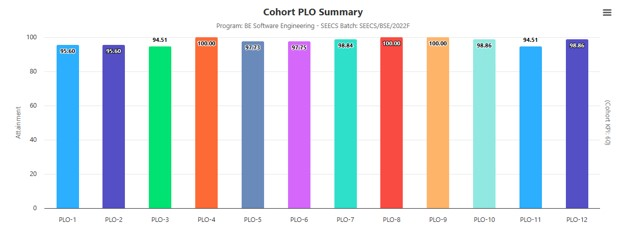
\includegraphics[width=0.8\textwidth]{images/criterion_8/media/Picture2.jpg}
    \caption{Cohort PLO Attainment from CLOs}
    \label{fig:sample9}
\end{figure}

\begin{figure}[H]
    \centering
    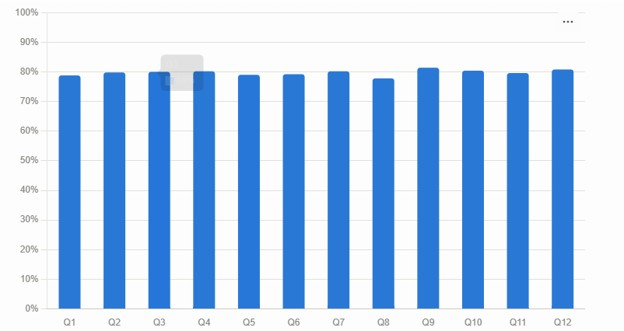
\includegraphics[width=0.8\textwidth]{images/criterion_8/media/Picture4.jpg}
    \caption{Cohort PLO Attainment from Exit Survey}
    \label{fig:sample10}
\end{figure}

\begin{figure}[H]
    \centering
    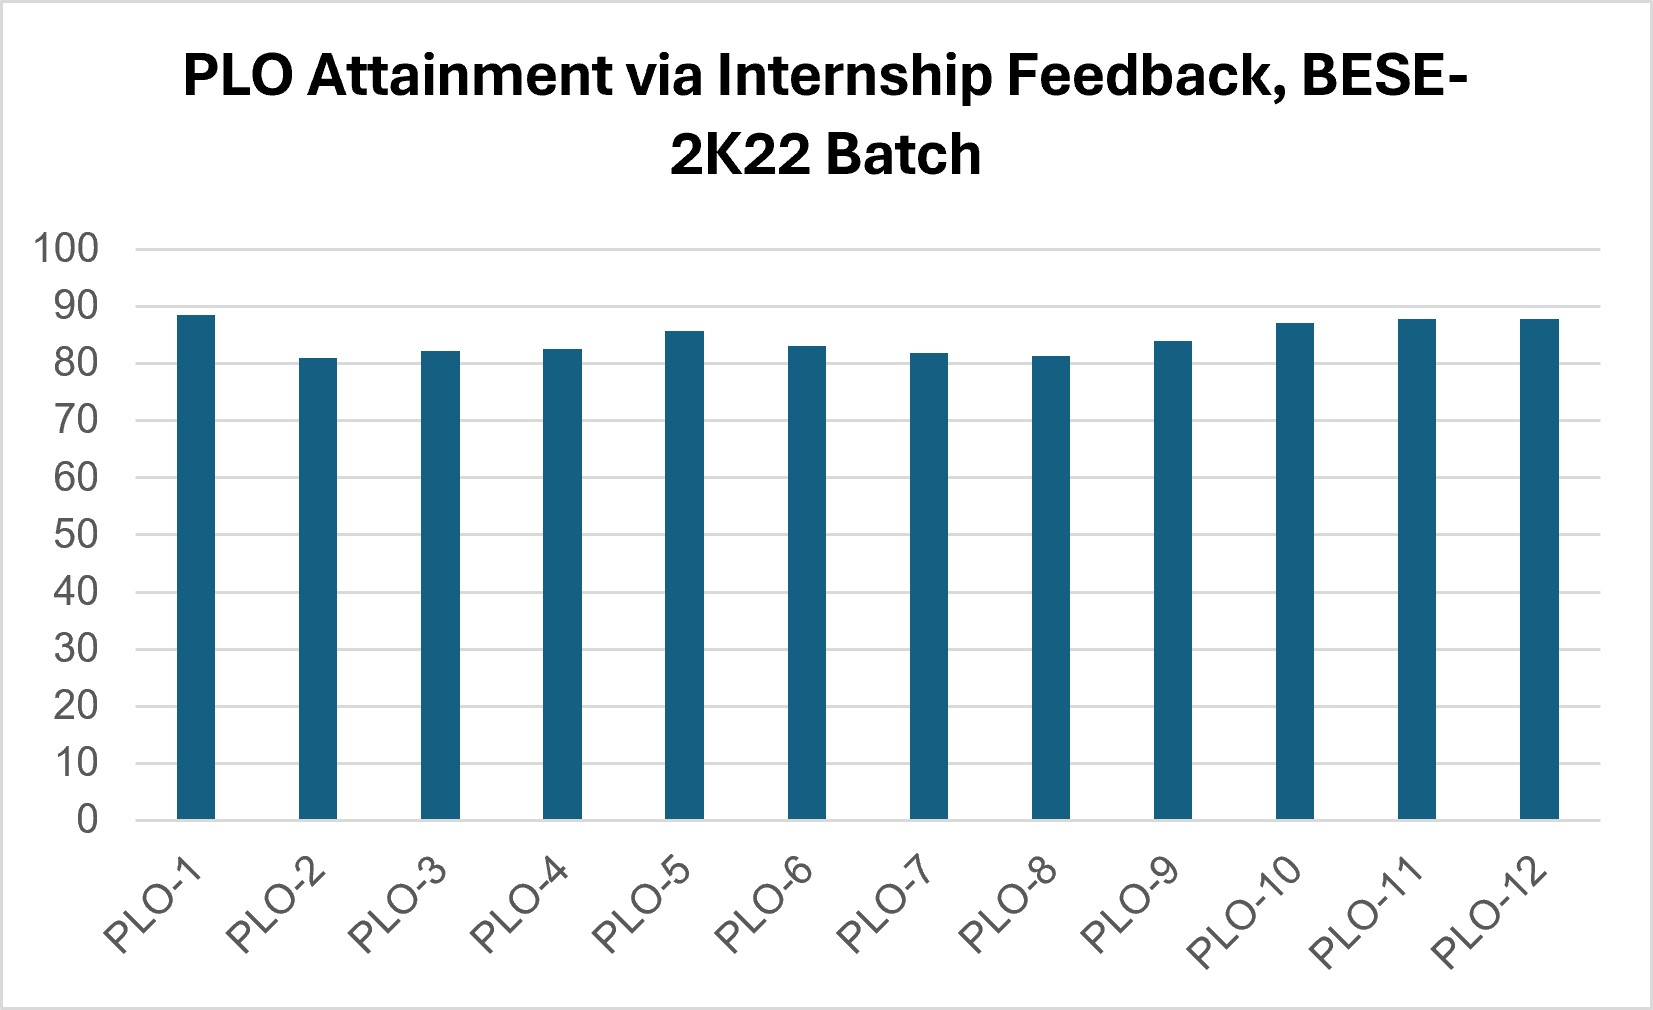
\includegraphics[width=0.8\textwidth]{images/criterion_8/media/Picture5.jpg}
    \caption{Cohort PLO Attainment from Internship Feedback}
    \label{fig:sample11}
\end{figure}

The graphs indicate that the Cohort-Level PLO attainment has achieved the prescribed threshold of 60\% in all three assessments. Accordingly, no CQI intervention is warranted at the cohort level.
Following the observations made by the PEC evaluation team during the previous accreditation visit, the internship feedback forms were reviewed by the Departmental Continuous Quality Improvement (CQI) Committee. The committee analyzed the existing feedback mechanism, considered the evaluators' concerns, and recommended appropriate revisions to improve the effectiveness and comprehensiveness of the internship feedback process. The revised feedback forms were subsequently implemented as part of the department's continuous quality improvement initiatives. The revised system is explained in detail in Criteria 2.

\hypertarget{criterion-8-clos}{%
\section{CLOs}\label{criterion-8-clos}}

\hypertarget{criterion-8-cqi-process-for-clos}{%
\subsection{CQI Process for CLOs}\label{criterion-8-cqi-process-for-clos}}

The innermost loop of OBE implementation model deals with CQI process for CLOs (coursework). The faculty and DLQEC are responsible for CQI of CLOs as shown in Figure~\ref{fig:cqi-clo}. CLOs are directly assessed through coursework and laboratory work involving examination and rubrics. The data is collected, evaluated, and reviewed at the end of every semester. 

\begin{figure}[H]
\centering
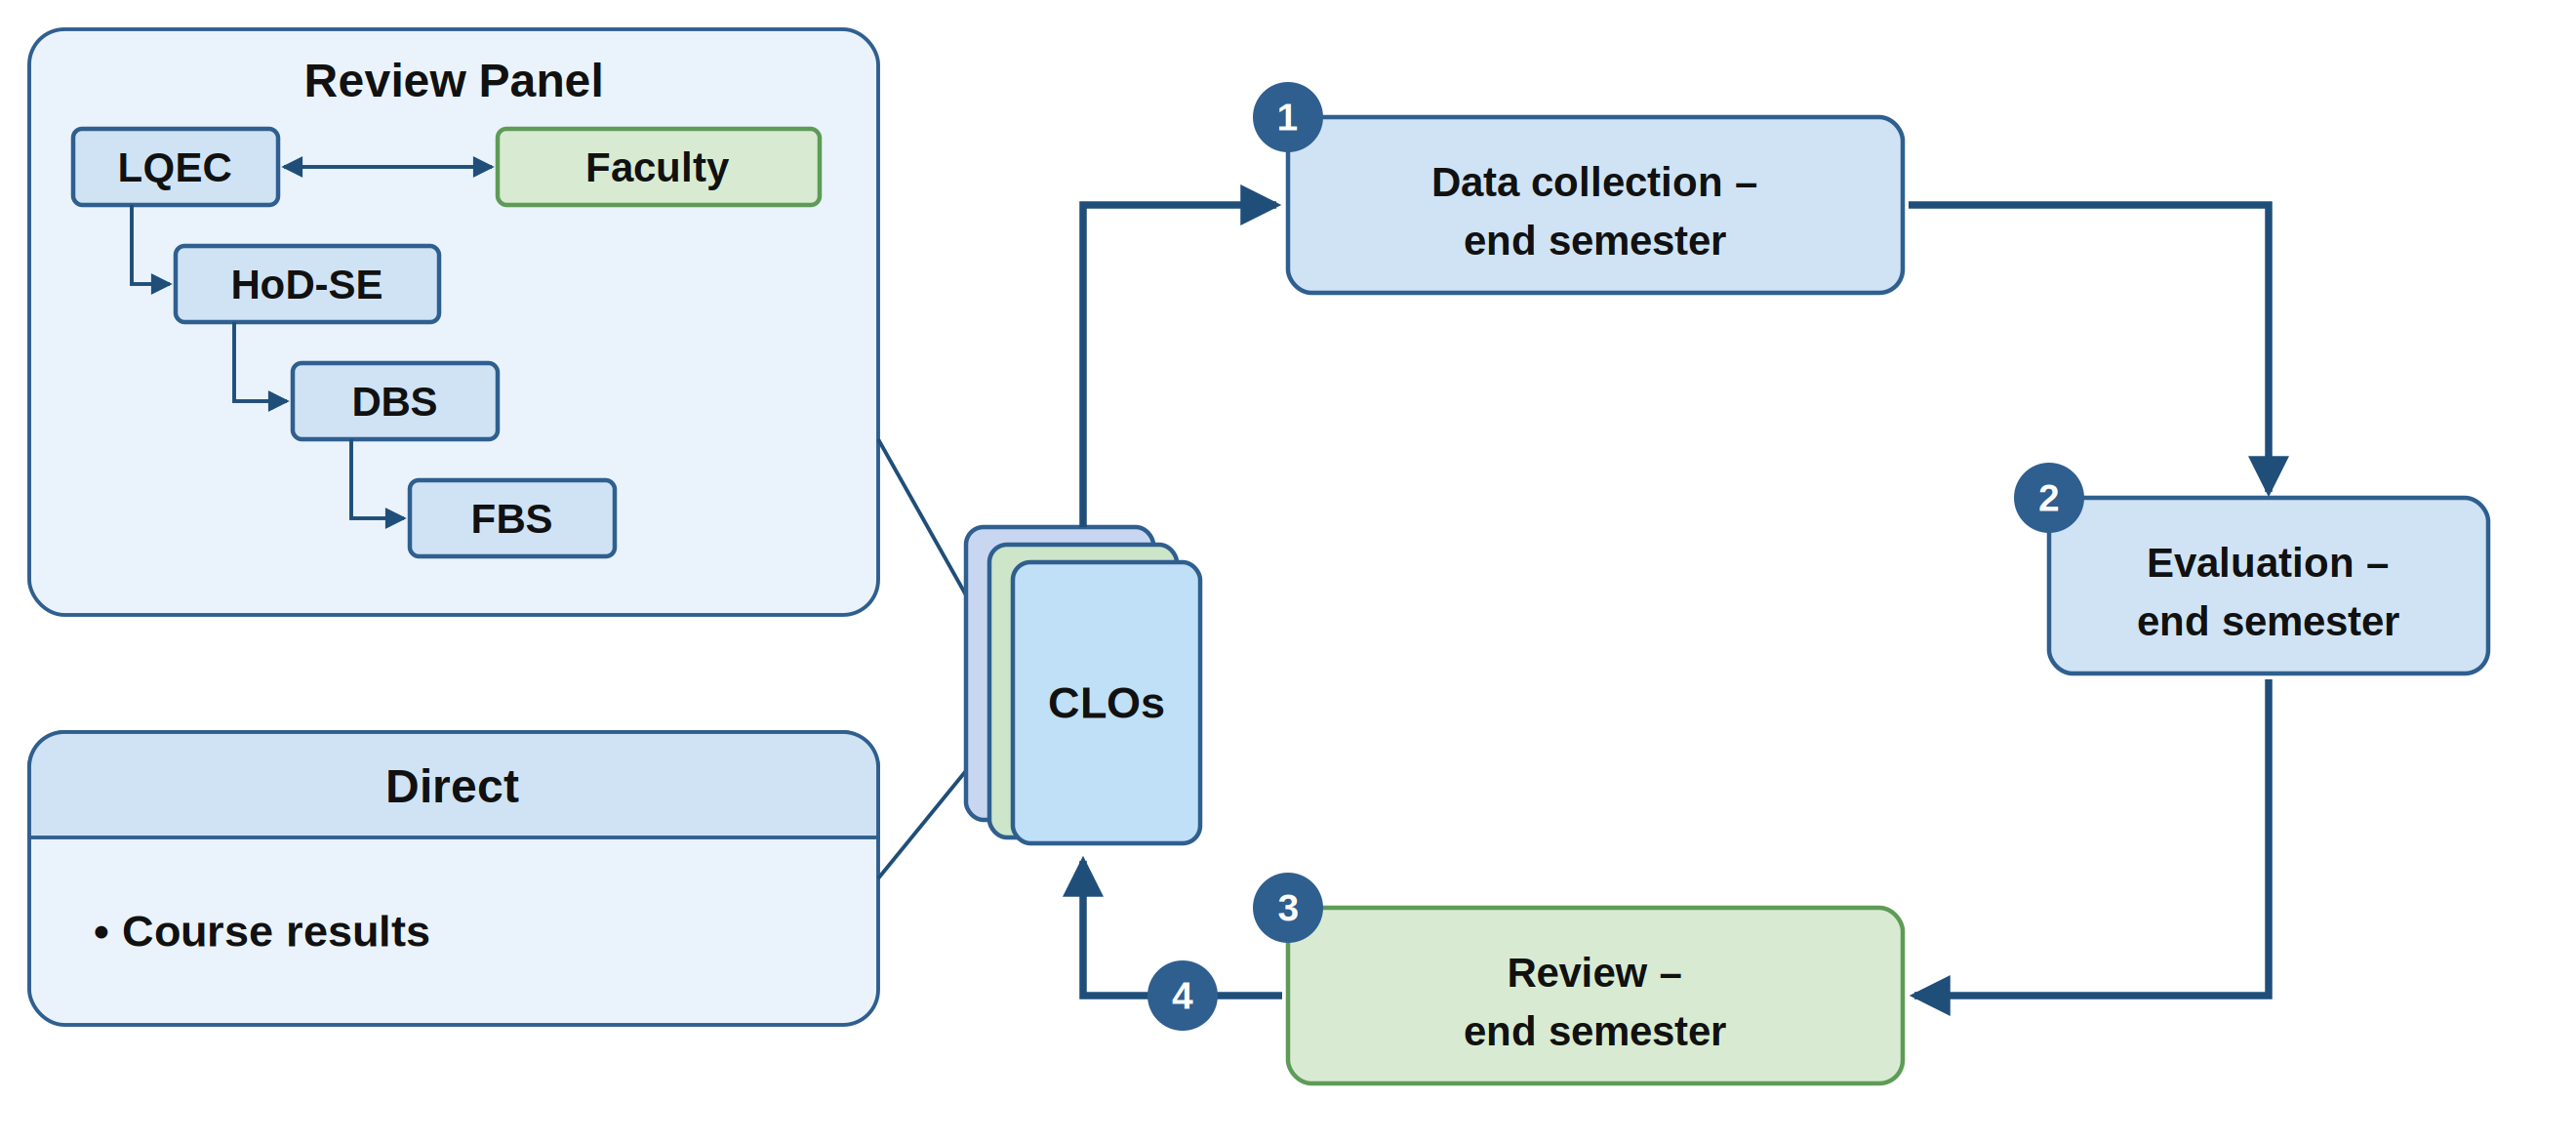
\includegraphics[width=1.0\textwidth]{images/front_matter/media/image-18.png}
\caption{CQI Process for CLOs}
\label{fig:cqi-clo}
\end{figure}

\hypertarget{criterion-8-review-and-corrective-action-processes-for-clos}{%
\subsection{Review and Corrective Action Processes for CLOs}\label{criterion-8-review-and-corrective-action-processes-for-clos}}

Course Learning Outcomes are continuously monitored and evaluated through CLO-attainment analysis and the Course Review Report as part of the department's Continuous Quality Improvement process. The DLQEC reviews Course Learning Outcome attainment, mapping of Course Learning Outcomes to Program Learning Outcomes, Bloom's Taxonomy levels, and learning domains to evaluate the effectiveness of course delivery and assessment. Based on this review, recommendations are made for improvement and are subsequently discussed and approved by the CQI Committee and Departmental Board of Studies. The Knowledge Group Heads also review course outlines, the course materials and taxonomy levels before the start of each semester. Incase of any improvement suggested by the KGH, the improvements are reviewed by CQI committee and corrective actions and initiated through corrective action forms. The approved actions may include revisions to the mapping of Course Learning Outcomes to Program Learning Outcomes, Bloom's Taxonomy levels and assessment methods.
\begin{figure}[H]
\centering
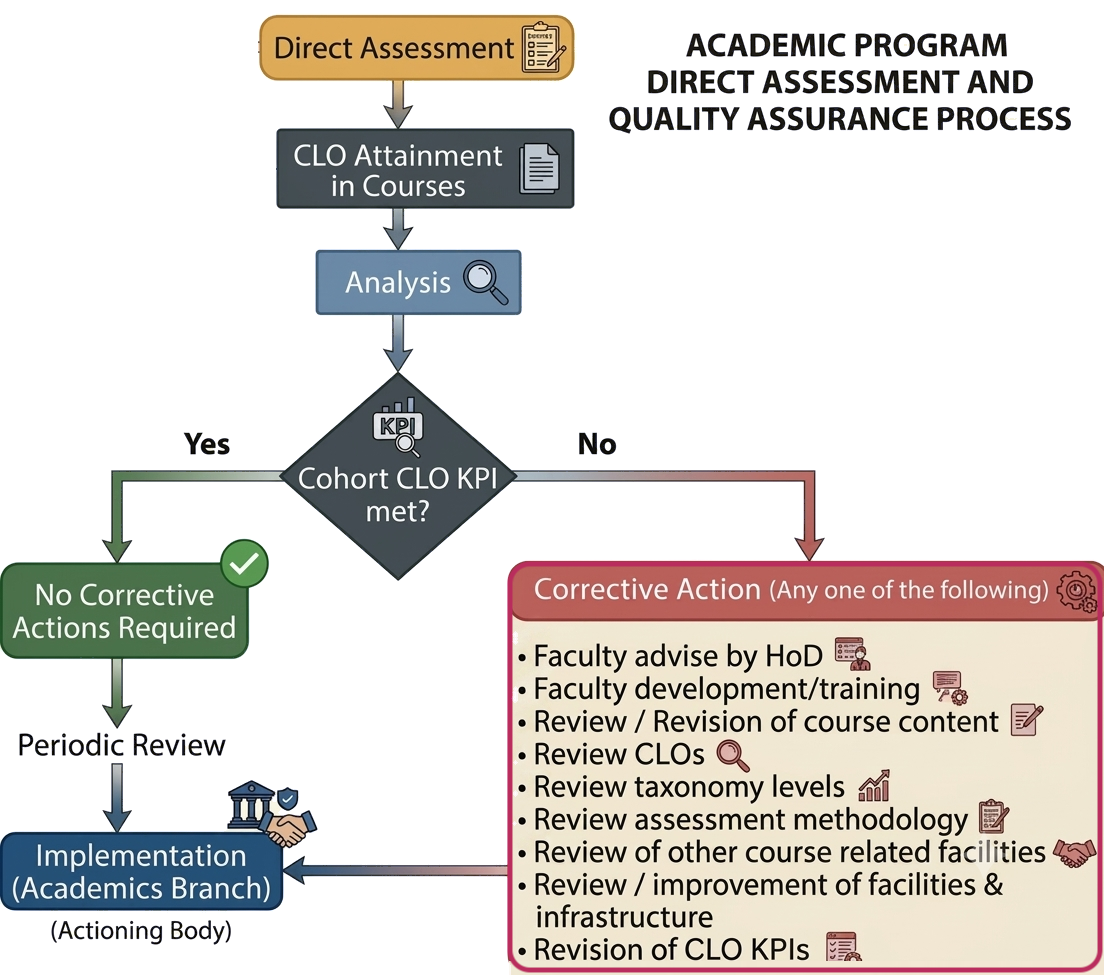
\includegraphics[width=5.18in,height=4.89in]{images/front_matter/media/image-19.png}
\caption{Corrective Actions for CLOs}
\label{fig:corrective-CLOs}
\end{figure}

The Course Learning Outcome review process begins with the measurement of Course Learning Outcome attainment through quizzes, assignments, laboratory work, sessional assessments, and the end-semester examination. Figure~\ref{fig:corrective-CLOs} illustrates the complete process for monitoring and improving Course Learning Outcome attainment. If the cohort-level attainment of a Course Learning Outcome is 60\% or above, the established Key Performance Indicator is considered achieved, and no corrective action is required. However, if the cohort-level attainment falls below 60\%, the Local Quality Enhancement Cell, in consultation with the course instructor and the relevant faculty members, initiates the Continuous Quality Improvement process to identify the underlying causes and recommend appropriate corrective measures. 

Depending on the identified issues, corrective actions may include guidance from the Head of Department, faculty development and training, revision of Course Learning Outcomes, review of Bloom's Taxonomy levels, improvement of assessment methods, enhancement of course delivery practices, and review of laboratory resources and equipment. Nevertheless, if the DLQEC identifies any gaps in CLO coverage, or faculty understanding, appropriate corrective actions are initiated to address the identified shortcomings and further strengthen the effectiveness of the process as part of the department's continuous quality improvement initiatives. The implementation of all the approved corrective actions for improvement of courses is carried out through approval of DBS. Table~\ref{tab:cqi_actions} lists some of the corrective actions taken to improve the CLOs and their mappings.

\begin{table}[ht]
\centering
\footnotesize
\setlength{\tabcolsep}{4pt}
\label{fig:sample12}
\begin{tabular}{
>{\raggedright\arraybackslash}p{4cm}
>{\raggedright\arraybackslash}p{2cm}
>{\raggedright\arraybackslash}p{3cm}
>{\raggedright\arraybackslash}p{2.8cm}
>{\raggedright\arraybackslash}p{3cm}
}
\toprule
\textbf{Observation} &
\textbf{Source} &
\textbf{Action Taken} &
\textbf{Evidence} \\
\midrule
Revision of CLOs &
KGH  &
Updated Course Outline &
Corrective Action form and DBS minutes in Annex ~\ref{annex:oop} \\

Revision of BT Levels &
Faculty Course Review Report &
Revised BT Levels in outline &
Corrective Action form and DBS minutes \\

CLO Coverage &
DLQEC &
Faculty Training and Course Outline Revision &
Meeting Minutes and Training Feedback \\

\bottomrule
\end{tabular}
\caption{Examples of CQI Activities for CLOs}
\label{tab:cqi_actions}
\end{table}

\hypertarget{Stakeholders Feedback Mechanism}{%
\section{Stakeholders Feedback Mechanism}\label{Stakeholders-Feedback-Mechanism}}

Stakeholder engagement is a fundamental component of the Department's Continuous Quality Improvement (CQI) framework. To ensure that the program remains relevant, effective, and aligned with accreditation requirements and industry needs, the Department systematically collects and analyses feedback from students, alumni, employers, faculty members, and the Industrial Advisory Board. Since each stakeholder offers a distinct perspective on program quality, their feedback is incorporated at appropriate decision-making levels to support evidence-based improvements in curriculum, teaching and learning, assessment practices, and overall program management. This structured approach ensures that improvement initiatives are responsive to stakeholder expectations and are continuously monitored for their effectiveness.

\begin{table}[!t]
\centering
\scriptsize                 % Changed from \footnotesize
\renewcommand{\arraystretch}{1.0}   % Reduce row height
\setlength{\tabcolsep}{3pt}         % Reduce column padding
\caption{Stakeholder Inputs and Their Role in Continuous Quality Improvement}

\begin{tabular}{
>{\raggedright\arraybackslash}p{2.6cm}
>{\raggedright\arraybackslash}p{2.6cm}
>{\raggedright\arraybackslash}p{2.5cm}
>{\raggedright\arraybackslash}p{3.8cm}
>{\raggedright\arraybackslash}p{2.6cm}
}
\toprule
\textbf{Stakeholder} &
\textbf{Primary Input} &
\textbf{Decision Level} &
\textbf{CQI Outcome} &
\textbf{Evidence} \\
\midrule

Students &
Course evaluations, student advisory system, exit surveys &
Course and Department Level &
Improvements in course delivery, assessment methods, labs, learning resources and student support &
Survey reports \\
\addlinespace

Faculty &
Course reviews, faculty audit, departmental meetings &
Course and Curriculum Level &
Revision of CLOs, assessment strategies, teaching methods, lab Manuals and course sequencing &
Corrective Action Forms, course review records \\
\addlinespace

Alumni &
Alumni surveys&
Program Level &
Identification of curriculum gaps, emerging skill requirements and enhancement of graduate attributes &
Alumni survey reports\\
\addlinespace

Employers &
Employer surveys, internship evaluations &
Program and Curriculum Level &
Strengthening technical competencies, professional skills, industry alignment and internship improvements &
Employer survey reports, internship feedback reports \\
\addlinespace

Industrial Advisory Board (IAB) &
Recommendations during advisory meetings &
Strategic Program Level &
Curriculum revision, emerging technologies, industry collaboration, new electives and strategic improvements &
Meeting minutes, attendance records, recommendation logs \\
\addlinespace

Pakistan Engineering Council (PEC) &
Accreditation observations and recommendations &
Institutional and Program Level &
Compliance with accreditation requirements, OBE implementation, curriculum restructuring and assessment enhancement &
Accreditation reports, compliance records \\
\addlinespace

Higher Education Commission (HEC) &
Academic policies, curriculum guidelines and quality assurance requirements &
Institutional and Curriculum Level &
Compliance with national policies, credit hour adjustments and curriculum standardization &
HEC policies, implementation records \\
\bottomrule
\end{tabular}

\label{tab:stakeholder_cqi}
\end{table}

\hypertarget{Implementation Plan of Previous Accreditation Observations}{%
\section{Implementation Status of Previous Accreditation Observations}\label{Implementation-Status-of-Previous-Accreditation-Observations}}

The Department is committed to fostering a culture of Continuous Quality Improvement by systematically addressing observations and recommendations from the previous PEC accreditation visit. Since the last evaluation, sustained efforts have been made to strengthen academic and administrative processes, enhance assessment and quality assurance systems, empower faculty through professional development and active participation, and improve overall program effectiveness. The implementation of these corrective actions has been regularly monitored through the department's CQI mechanism. A summary of the implementation status of the observations and the corresponding remedial actions is presented in the Annexure~\ref{annex:rejoinder}.
 \hypertarget{New Facilities Added}{%
\section{New Facilities Added}\label{new-facilities}}

With the completion of the New Academic Block shown in Figure~\ref{fig:sample13}, the Department's infrastructure has been significantly enhanced, providing improved facilities to better support teaching, learning, research, and academic activities for both students and faculty.
\begin{figure}[H]
    \centering
    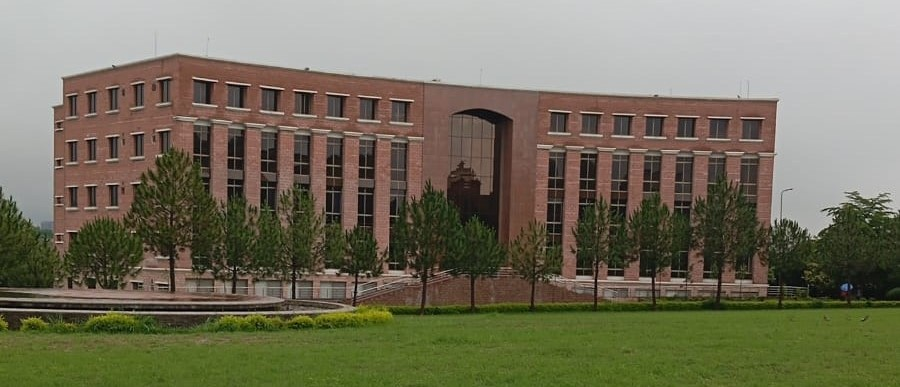
\includegraphics[width=0.6\textwidth]{images/criterion_8/media/acad_block.jpeg}
    \caption{New Academic Block}
    \label{fig:sample13}
\end{figure}

Table~\ref{tab:infrastructure} provides the summary of new facilities added.

\begin{table}[h]
  \centering
  \caption{SEECS infrastructure (existing blocks and New Academic Block)}
  \label{tab:infrastructure}
  \small
  \begin{tabular}{|>{\raggedright\arraybackslash}p{0.39\textwidth}|>{\centering\arraybackslash}p{0.13\textwidth}|>{\centering\arraybackslash}p{0.15\textwidth}|>{\centering\arraybackslash}p{0.10\textwidth}|}
    \hline
    \textbf{Infrastructure} & \textbf{Existing blocks*} & \textbf{New Academic Block} & \textbf{Total} \\
    \hline
    Classrooms                            & 22      & 14      & 36       \\ \hline
    Offices -- Faculty / Officers         & 109     & 26      & 135      \\ \hline
    Principal / Assoc.\ Dean / HoD Offices & 6      & 10      & 16       \\ \hline
    Conference Rooms                      & 3       & 1       & 4        \\ \hline
    Faculty Lounges                       & 2       & 1       & 3        \\ \hline
    Common Rooms (male / female)          & 3       & 2       & 5        \\ \hline
    Exam Branch / Archive Room            & 1       & 1       & 2        \\ \hline
    Other Offices (IT/ACB/Admin/PA)       & 2/2/3/6 & 1/1/1/7 & 3/3/4/13 \\ \hline
  \end{tabular}

  \vspace{2pt}
  {\footnotesize *Existing blocks: UG/PG SEECS blocks, RIMMS and IESE.\par}
  
\end{table}


 \hypertarget{New Initiatives Since Last Accreditation Visit}{%
\section{New Initiatives Since Last Accreditation Visit}\label{new-initiatives}}
The Department has undertaken several strategic initiatives to strengthen the implementation of Outcome-Based Education (OBE) and continuously improve its assessment, evaluation, academic processes, and learning environment. The details of initiatives taken after the last visit are mentioned in the following sections.

\hypertarget{Revised-Assessment-Instruments}{%
\subsection{Revised Assessment Instruments}\label{revised-assesment-instrument}}

\subsubsection{New Alumni Survey (2026)}
The legacy Alumni Survey (9 items, comprising a mix of Likert-scale
and binary Yes/No questions) was fully redesigned following two triggers:
(a) the 2023 PEC accreditation visit flagged poor correlation in PEO-2
and PEO-3 sub-KPI items; and (b) the IAB session held in November 2023
flagged that legacy item 5 inadequately measured PEO-2 attainment.

\begin{itemize}[noitemsep, topsep=0pt]
    \item \textbf{Old form:} 9 items; 4 binary Yes/No questions;
    weak PEO alignment; rigid all-or-nothing pass rule.

    \item \textbf{New form:} 12 items on a 5-point Likert scale (0--4);
    4 items per PEO; each item directly and exclusively mapped to one PEO.

    \item \textbf{Approval trail:} DBS, 20 April 2026
    $\rightarrow$ FBS, 21 April 2026
    $\rightarrow$ IAB endorsement, 5 May 2026.

    \item \textbf{2026 results:} 79 alumni responses;
    PEO-1: 0.803, PEO-2: 0.797, PEO-3: 0.803.
    All three PEOs were attained.
\end{itemize}

\subsubsection{New Employer Survey (2026)}
The Employer Survey was redesigned in parallel with the Alumni Survey.
The revised survey comprises 12 items on a 5-point Likert scale, with
4 items per PEO and an observer-assessment framing. The previous
version contained 7 loosely mapped items. A total of 50 employer
responses were received during the 2026 cycle.

\subsubsection{Redesigned Graduate Exit Survey}
\begin{itemize}[noitemsep, topsep=0pt]
    \item \textbf{Old form:} Generic Likert-scale questions with
    limited traceability to Program Learning Outcomes (PLOs).

    \item \textbf{New form:} Each question is mapped directly to a
    specific PLO. The survey is structured to reduce acquiescence
    bias and is administered through the Learning Management System (LMS).

    \item \textbf{Results:} Batches 2K20, 2K21, and 2K22 consistently
    show mean scores near or above 4.0/5.0 across all PLOs.
\end{itemize}

\subsubsection{Revised Internship Employer Feedback Form}
\begin{itemize} [noitemsep, topsep=0pt]
    \item \textbf{Redesigned:} All items are now mapped to relevant PLOs, providing traceable indirect evidence. 

    \item \textbf{Automated via TMS:} The Online Internship Feedback
    Module, integrated into the Thesis Management System (TMS),
    replaces the previous manual email process.

    \item \textbf{Dual evaluation:} Internships are now assessed through
    both employer feedback submitted via TMS and faculty assessment,
    providing a more comprehensive picture of student performance.
\end{itemize}




\subsection{PLOs Reduced from 12 to 11 (Batch 2K24 Onwards)}
\label{plo-reduction-12-to-11}

The Program Learning Outcomes (PLOs) have been reduced from 12 to 11,
effective from Batch 2K24 onwards, in alignment with the latest PEC
Manual of Accreditation and HEC Undergraduate Education Policy (UEP-2024).
The key structural change involves merging the former PLO-6
(\textit{Engineer and Society}) and PLO-7
(\textit{Environment and Sustainability}) into the revised PLO-6
(\textit{Engineer and the World}).

Table~\ref{tab:plo-revision} summarizes the changes between the previous
PLO framework applicable to batches up to 2K23 and the revised framework
applicable from Batch 2K24 onwards.

\begin{longtable}{|p{0.27\textwidth}|p{0.30\textwidth}|p{0.35\textwidth}|}
\hline
\textbf{Old PLO (till Batch 2K23)} &
\textbf{New PLO (Batch 2K24 and onwards)} &
\textbf{Change} \\
\hline
\endfirsthead

\hline
\textbf{Old PLO (till Batch 2K23)} &
\textbf{New PLO (Batch 2K24 and onwards)} &
\textbf{Change} \\
\hline
\endhead

PLO-1: Engineering Knowledge &
PLO-1: Engineering Knowledge &
Wording streamlined. \\
\hline

PLO-2: Problem Analysis &
PLO-2: Problem Analysis &
Minor update. \\
\hline

PLO-3: Design/Development &
PLO-3: Design/Development &
Unchanged. \\
\hline

PLO-4: Investigation &
PLO-4: Investigation &
Reframed as ``conduct investigation''. \\
\hline

PLO-5: Tool Usage &
PLO-5: Tool Usage &
Unchanged. \\
\hline

PLO-6: Engineer and Society; PLO-7: Environment and Sustainability &
PLO-6: Engineer and the World &
\textbf{Merged:} combines societal and sustainability perspectives. \\
\hline

PLO-8: Ethics &
PLO-7: Ethics &
Expanded to include diversity, inclusion, and international laws. \\
\hline

PLO-9: Teamwork &
PLO-8: Teamwork &
Expanded to include remote and distributed settings. \\
\hline

PLO-10: Communication &
PLO-9: Communication &
Expanded to address cultural and language differences. \\
\hline

PLO-11: Project Management &
PLO-10: Project Management and Finance &
Expanded to include economic decision-making. \\
\hline

PLO-12: Lifelong Learning &
PLO-11: Lifelong Learning &
Expanded to cover learning, adaptability, and critical thinking. \\
\hline
\caption{Comparison of Previous and Revised PLO Frameworks}
\label{tab:plo-revision}\\
\end{longtable}

The revised framework retains the core engineering competencies while
consolidating societal and sustainability considerations into a single
outcome. The remaining outcomes have been renumbered accordingly, with
several also expanded to reflect broader professional and contemporary
engineering requirements.

\subsection{Curriculum Revisions}
\label{subsec:curriculum-revisions}

\subsubsection{Three Working Papers Since Last PEC Visit}
\label{subsubsec:working-papers}

\begin{longtable}{|p{4.0cm}|p{3.5cm}|p{7.5cm}|}
\hline
\textbf{Working Paper} &
\textbf{Applicable From} &
\textbf{Reason / Key Changes} \\
\hline
\endfirsthead

\hline
\textbf{Working Paper} &
\textbf{Applicable From} &
\textbf{Reason / Key Changes} \\
\hline
\endhead

WP No.~30, 64th ACM
\newline 23 January 2023
&
Batch 2K19--2K23
\newline (Fall 2019 onwards)
&
FYDP credit redistribution: 7th semester
from 3 CH to 2 CH, and 8th semester
from 3 CH to 4 CH. This change was
required by NUST's minimum semester
load policy. \\
\hline

WP No.~20, 69th ACM
\newline 6 August 2024
&
Batch 2K24
\newline (Fall 2024 onwards)
&
PEC--HEC UEP-2023 compliance:
English courses added; Pakistan Studies
replaced with Ideology and Constitution
of Pakistan; Ethics introduced for
non-Muslim students; and semester
credit-hour distribution adjusted. PLOs reduced
from 12 to 11.\\
\hline

WP No.~30, 72nd ACM
\newline 4 September 2025
&
Batch 2K25
\newline (Fall 2025 onwards)
&
PEC--HEC UEP-2024 compliance:
compulsory Pakistan Studies and
Fehm-e-Quran-I and II introduced in the
Non-Engineering domain. Engineering electives
increased from 5 to 6. \\
\hline
\end{longtable}


\subsubsection{New and Modified Courses}
\label{subsubsec:new-modified-courses}

\begin{itemize}[noitemsep, topsep=0pt]

    \item \textbf{New Elective --- Virtual and Augmented Reality (CS-365):}
    Introduced to provide students with exposure to extended reality (XR)
    and emerging technologies.

    \item \textbf{New Elective --- Introduction to Quantum Computing:}
    Introduced in response to the recommendation of the Industrial
    Advisory Board (IAB).

    \item \textbf{Fundamentals of Computer Programming (CS-110):}
    Credit hours increased from 3 to 4 CH to strengthen students'
    programming foundations, following IAB recommendations.

    \item \textbf{Engineering Electives:}
    The number of engineering electives increased from 5 to 6,
    providing students with greater flexibility in course selection.

    \item \textbf{Removed Courses:}
    Workshop Practice and Engineering Drawing were removed from the
    common first-year curriculum to sharpen the discipline-specific
    focus.

    \item \textbf{Certification-Style Courses (In Progress):}
    NUST WP No.~2, 73rd ACM, dated 9 February 2026, was approved
    and endorsed at UCAP on 30 January 2026. The initiative will
    recognize 1--3 CH per departmentally validated certification.
    Implementation is awaiting the final Standard Operating
    Procedure (SOP) from the PEC Engineering Accreditation Board.

\end{itemize}


\subsubsection{CEP and OEL Formalised}
\label{subsubsec:cep-oel}

\begin{itemize}[noitemsep, topsep=0pt]

    \item \textbf{Complex Engineering Problems (CEP) Policy:}
    A formal departmental policy has been documented, requiring
    all courses with laboratory work or projects to incorporate
    Complex Engineering Problems.

    \item \textbf{Open-Ended Laboratory (OEL) Activities:}
    Open-Ended Laboratory activities have been institutionalised
    in accordance with PEC requirements. Students define their
    own methodologies, justify their decisions, and validate
    their solutions rather than merely following predefined
    procedures.

\end{itemize}




\subsection{New Internship Mechanism}
\label{subsec:new-internship-mechanism}

\begin{itemize}[noitemsep, topsep=0pt]

    \item \textbf{Mandatory Graduation Requirement:}
    Internship is now compulsory for all BESE students.
    The degree cannot be awarded without successful completion
    of the internship requirement.

    \item \textbf{Automated Process via TMS:}
    The Online Internship Feedback Module has been introduced
    in the Thesis Management System (TMS), replacing the
    previous manual email-based feedback collection process.

    \item \textbf{Dual Evaluation Mechanism:}
    Internship evaluation incorporates both employer feedback
    submitted through TMS and faculty assessment, providing
    a more comprehensive evaluation of student performance.

    \item \textbf{PLO-Aligned Feedback Form:}
    The revised internship feedback form maps each question
    to a specific Program Learning Outcome (PLO), providing
    traceable indirect evidence for assessing PLO attainment.

    \item \textbf{ILO/NPO Coordination:}
    The Industrial Liaison Office (ILO) and NUST Placement
    Office (NPO) maintain a database of industry partners.
    Internship placements are arranged for 100\% of
    undergraduate students, with placements made as close
    to students' homes as possible.

\end{itemize}

\subsection{New PEO Evaluation Framework}
\label{subsec:new-peo-evaluation-framework}

The Program Educational Objectives (PEO) evaluation framework
was comprehensively revised in 2026, replacing the legacy
Key Performance Indicator (KPI) system with a transparent,
multi-step evaluation mechanism based on normalised scoring.

\begin{longtable}{|p{6.2cm}|p{8.8cm}|}
\hline
\textbf{Legacy Framework (Before 2026)} &
\textbf{New Framework (2026)} \\
\hline
9 alumni survey items and 7 employer survey items.
&
12 alumni survey items and 12 employer survey items,
with 4 items mapped to each PEO in each survey. \\
\hline

A combination of Likert-scale and binary Yes/No questions.
&
A uniform 5-point Likert scale, ranging from
0 (Strongly Disagree) to 4 (Strongly Agree). \\
\hline

Rigid evaluation mechanism requiring all sub-KPIs to meet
their respective thresholds individually.
&
A three-step evaluation mechanism:
\begin{enumerate}
    \item Question-level KPI score $\geq 2.0$.
    \item At least 3 out of 4 indicators for each PEO must pass.
    \item Normalised PEO score $\geq 0.60$.
\end{enumerate}
\\
\hline

The binary Yes/No question on pursuing higher education
penalised working graduates who had not pursued further studies.
&
All 8 indicators carry equal weight of 0.25, with no
binary Yes/No items.
\\
\hline

PEO-1 failed to meet the threshold because 36\% of alumni
were pursuing higher education, below the required 50\%
threshold.
&
The 2026 pilot evaluation demonstrated the attainment
of all three PEOs, with normalised scores of 0.803,
0.797, and 0.803, respectively.
\\
\hline
\end{longtable}


\subsection{Infrastructure \& Facilities}
\label{subsec:infrastructure-facilities}

\subsubsection{New Academic Block}
\label{subsubsec:new-academic-block}

A new Academic Block has been completed at SEECS,
significantly expanding the department's physical
infrastructure and providing additional facilities
for teaching, research, administration, and student support.

\subsubsection{Lab Procurement and Upgrades}
\label{subsubsec:lab-procurement-upgrades}

The department has continued to modernise its laboratory
infrastructure through hardware procurement and equipment
upgrades to support teaching, practical learning, and research.

\begin{itemize}[noitemsep, topsep=0pt]

    \item \textbf{Recent Procurement:}
    A total of 45 new personal computers (PCs) were purchased,
    and 50 existing PCs were upgraded with the latest hardware.

    \item \textbf{Lab Equipment Investment:}
    An investment of Rs.~71.55 million was made in 2024--25,
    followed by Rs.~74.82 million in 2025--26, reflecting
    continued investment in laboratory modernisation.

    \item \textbf{Current Laboratory Facilities:}
    The department currently operates 12 computer laboratories,
    one FYDP laboratory, and one Basic Electronics Laboratory.

\end{itemize}


\subsubsection{Network and Connectivity}
\label{subsubsec:network-connectivity}

The department provides network connectivity and computing
facilities to support academic activities, research, and
access to digital resources.

\begin{itemize}[noitemsep, topsep=0pt]

    \item \textbf{Bandwidth:}
    A bandwidth allocation of 910 Mbps is provided through
    PERN via the NUST Campus Core Network, with an additional
    7 Mbps backup connection for research laboratories.

    \item \textbf{Remote Access:}
    A Virtual Private Network (VPN) server hosted at SEECS
    enables secure remote access to campus computing resources.

    \item \textbf{Library Facilities:}
    The library provides high-speed DSL connectivity and Wi-Fi,
    bookable group study rooms, a seminar hall, a conference
    room, and laptop charging points.

\end{itemize}


\subsubsection{Student Support Services: New Initiatives}
\label{subsubsec:student-support-services}

Several initiatives have been introduced to improve student
facilitation, psychological well-being, career development,
and access to support services across NUST.

\begin{itemize}[noitemsep, topsep=0pt]

    \item \textbf{NUST Student Support Services Centre (S3C):}
    A centralised, one-window facilitation platform has been
    introduced to manage student requests and provide access
    to support services across the campus.

    \item \textbf{Centre for Counselling and Career Advisory (C3A):}
    The centre provides professional psychological counselling
    services to the NUST community. Its services include IQ,
    EQ, personality, aptitude, career-interest, stress, and
    depression assessments. The centre is staffed by
    qualified psychologists.

    \item \textbf{Career Development Centre (CDC):}
    The centre provides employability programmes, networking
    events, employer engagement activities, and curriculum
    support. It also coordinates closely with the NUST
    Placement Office to strengthen students' career readiness
    and employment prospects.

\end{itemize}


\subsection{Faculty Development \& Training}
\label{subsec:faculty-development-training}

The department promotes continuous faculty development through
structured training, mentoring, professional development
opportunities, and initiatives aimed at strengthening
Outcome-Based Education (OBE) practices and the academic
environment.

\begin{itemize}[noitemsep, topsep=0pt]

    \item \textbf{OBE Induction:}
    All newly inducted faculty members undergo mandatory pedagogical training (including OBE) at NUST Center for Teaching and Learning (NCTL). The training covers Course Learning Outcome
    (CLO) formulation, Bloom's Taxonomy, and mapping of CLOs
    to Program Learning Outcomes (PLOs).

    \item \textbf{Mentoring System:}
    Each newly inducted faculty member is paired with a
    senior faculty mentor during the first semester to
    facilitate professional integration, teaching support,
    and academic development.

    \item \textbf{Comprehensive OBE Training Sessions:}
    Additional OBE training sessions were conducted following
    the PEC 2023 visit, with particular emphasis on improving
    faculty understanding and application of taxonomy levels
    in teaching, assessment, and outcome evaluation.

    \item \textbf{Green Week:}
    A newly introduced initiative to promote faculty
    well-being and foster a positive, supportive, and
    healthy academic environment.

    \item \textbf{Financial Support for Faculty Development:}
    A dedicated allocation in the university's recurring
    budget supports faculty participation in conferences,
    professional certifications, and pedagogical training.

    \item \textbf{Professional Development Centre (PDC):}
    Established in 2007, the PDC serves as an International
    Finance Corporation (IFC), World Bank Group, management
    training partner and a PEC Continuing Professional
    Development (CPD) partner. It has trained more than
    3,500 professionals from over 450 organisations.

\end{itemize}

\subsection{CQI \& OBE System Enhancements}
\label{subsec:cqi-obe-system-enhancements}

The department has strengthened its Continuous Quality
Improvement (CQI) and Outcome-Based Education (OBE) systems
through formalised quality assurance procedures, enhanced
digital documentation, automated attainment reporting, and
individual student monitoring to ensure continuous
improvement in academic outcomes.

\begin{itemize}[noitemsep, topsep=0pt]

    \item \textbf{Dedicated CQI Committee:}
    A dedicated Continuous Quality Improvement (CQI) Committee
    has been formally established to review assessment results,
    monitor the implementation of corrective actions, and
    facilitate continuous improvement in academic processes
    and programme quality.

    \item \textbf{Enhanced Thesis Management System (TMS):}
    The Thesis Management System (TMS) has been enhanced
    to record and monitor industry-sponsored Final Year
    Design Projects (FYDPs), in addition to managing
    internship feedback. These enhancements provide a
    unified portal for project management and related
    academic monitoring activities.

    \item \textbf{Course and Laboratory Folders on LMS:}
    Mandatory digital documentation of all course and
    laboratory folders on the Learning Management System
    (LMS) ensures the long-term sustainability,
    accessibility, and availability of academic records
    for quality assurance and accreditation purposes.

    \item \textbf{Qalam OBE System:}
    Qalam, NUST's in-house campus management system,
    automatically generates semester-wise and batch-wise
    CLO and PLO attainment reports for all courses.
    These reports support systematic assessment,
    outcome monitoring, and evidence-based academic
    improvement.

\end{itemize}

\subsection{Industry Linkages \& Partnerships}
\label{subsec:industry-linkages-partnerships}

The department maintains strong linkages with industry,
research organisations, and national and international
partners to enhance curriculum relevance, promote
industry-oriented research, and strengthen collaboration
between academia and industry.

\begin{itemize}

    \item \textbf{Industrial Advisory Board (IAB):}
    Multiple IAB sessions were conducted between May 2023 and May 2026, resulting in 11 major recommendations, of which
    7 have been closed. Key completed recommendations
    include the introduction of new electives in Virtual
    and Augmented Reality (VR/AR) and Introduction to
    Quantum Computing, the increase in credit hours for
    Fundamentals of Computer Programming (FoCP), and the
    revision of Program Educational Objective (PEO)
    evaluation instruments.

    \item \textbf{Industry-Sponsored Final Year Design
    Projects (FYDPs):}
    Industry-sponsored FYDPs are co-supervised by SEECS
    faculty members and professionals from startups
    associated with the National Science and Technology
    Park (NSTP). The Thesis Management System (TMS) has
    been enhanced to formally record and monitor these
    projects, supporting systematic tracking and
    coordination.

    \item \textbf{International Research Collaborations:}
    The department maintains research collaborations
    with 81 international collaborators across
    28 countries, strengthening global research
    engagement, knowledge exchange, and opportunities
    for joint academic activities.

    \item \textbf{NUST Industry-Academia Ecosystem:}
    The department benefits from the active ecosystem
    of NUST centres and offices that facilitate
    industry engagement, entrepreneurship, technology
    transfer, research commercialisation, and
    professional development. These include the
    Centre for Advanced Computing (CAC), National
    Science and Technology Park (NSTP), Technology
    Incubation Centre (TIC), Office of Research,
    Innovation and Commercialisation (ORIC),
    Intellectual Property Office (IPO), Technology
    Transfer Office (TTO), Professional Development
    Centre (PDC), Career Development Centre (CDC),
    Industrial Liaison Office (ILO), and Global
    Technology and Technology Network (GTTN).
    Collectively, these entities support stronger
    linkages between academic research, industry
    requirements, entrepreneurship, and graduate
    employability.

\end{itemize}

\subsection{Quick-Reference Summary (All Initiatives)}
\label{subsec:quick-reference-summary}

\small
\renewcommand{\arraystretch}{1.2}

\begin{longtable}{|p{6.7cm}|p{1.8cm}|p{6.5cm}|}
\hline
\textbf{Initiative} & \textbf{Criterion} & \textbf{Status} \\
\hline
\endfirsthead

\hline
\textbf{Initiative} & \textbf{Criterion} & \textbf{Status} \\
\hline
\endhead

Revised Alumni Survey --- 12 items, 4 per PEO, 5-point Likert
& C1 / C8
& DONE --- DBS, FBS, and IAB approved, April--May 2026 \\
\hline

Revised Employer Survey --- 12 items mirroring alumni survey
& C1 / C8
& DONE --- Same approval cycle \\
\hline

New multi-step PEO evaluation (QL-KPI, coverage, normalised score)
& C1 / C8
& DONE --- Piloted in 2026; all 3 PEOs attained \\
\hline

PLOs reduced from 12 to 11 (PLO-6/7 merged; PLO-7 expanded with D\&I)
& C2 / C8
& DONE --- Effective Batch 2K24 onwards \\
\hline

Graduate Exit Survey redesigned (PLO-mapped, bias-reduced)
& C2 / C8
& DONE --- In use \\
\hline

Internship Employer Feedback Form redesigned (PLO-mapped)
& C2 / C3 / C8
& DONE --- Digitised via TMS \\
\hline

Internship made a mandatory graduation requirement
& C3 / C8
& DONE \\
\hline

Internship feedback automated via TMS Online Module
& C3 / C8
& DONE --- Replaces manual email collection \\
\hline

Dual internship evaluation --- employer and faculty
& C3 / C8
& DONE \\
\hline

Curriculum revision WP 64th ACM (2023) --- FYDP credit-hour redistribution
& C3
& DONE --- Batches 2K19--2K23 \\
\hline

Curriculum revision WP 69th ACM (2024) --- UEP-2023 compliance
& C3
& DONE --- Batch 2K24 \\
\hline

Curriculum revision WP No.~20, 69th ACM --- UEP-2024, PLOs 12 to 11
& C3
& DONE --- Batch 2K25 \\
\hline

New elective: Virtual and Augmented Reality (CS-365)
& C3
& ADDED \\
\hline

New elective: Introduction to Quantum Computing
& C3
& ADDED \\
\hline

Fundamentals of Computer Programming (CS-110) credit hours: 3 CH to 4 CH
& C3
& DONE \\
\hline

Engineering electives increased from 5 to 6
& C3
& DONE --- Batch 2K25 \\
\hline

Workshop Practice and Engineering Drawing removed
& C3
& DONE \\
\hline

Certification courses (1--3 CH per certification)
& C1 / C3
& PARTIAL --- Awaiting PEC EAB SOP \\
\hline

Formal CEP Policy documented and distributed 
& C3
& DONE \\
\hline

Open-Ended Laboratory (OEL) activities institutionalised per PEC 
& C3
& DONE \\
\hline

All course and laboratory folders mandated on LMS
& C3 / C8
& DONE \\
\hline

New Academic Block: 14 classrooms, 6 teaching labs, 26 offices
& C6 / C8
& COMPLETED \\
\hline

45 new PCs procured and 50 existing PCs upgraded
& C6
& DONE \\
\hline

Internet: 910 Mbps PERN, 7 Mbps backup, and VPN
& C6
& IN PLACE \\
\hline

S3C --- one-window student support centre
& C4 / C6
& OPERATIONAL \\
\hline

C3A --- professional psychological counselling centre
& C4 / C6
& OPERATIONAL \\
\hline

Career Development Centre (CDC) --- placement and employability
& C4 / C6 / C9
& OPERATIONAL \\
\hline

PDC one-week OBE induction for all newly inducted faculty
& C5 / C8
& ONGOING \\
\hline

Green Week --- faculty well-being initiative
& C8
& DONE \\
\hline

Dedicated CQI Committee established
& C8
& DONE \\
\hline

TMS enhanced to track industry-sponsored FYDPs
& C8 / C9
& DONE \\
\hline

Industry-sponsored FYDPs with NSTP startups
& C9
& ACTIVE \\
\hline

IAB: Multiple sessions (2023--2026), 1 recommendations, 4 closed
& C1 / C9
& ONGOING \\
\hline

International research collaborations: 81 partners across 28 countries
& C9
& ACTIVE \\
\hline

\end{longtable}

\normalsize
\renewcommand{\arraystretch}{1.0}
\clearpage

% ============================================================
% CHAPTER 10 — Criterion 9: Industrial Linkages
% Images: images/criterion_9/media/
% ============================================================
\graphicspath{{images/criterion_9/media/}}
% Criterion 9 converted from the supplied Word source.
% Expected packages: array, booktabs, longtable, graphicx, hyperref, calc, enumitem, float.
\providecommand{\real}[1]{#1}
\providecommand{\tightlist}{}

\hypertarget{criterion-9-industrial-linkages}{%
\chapter{Criterion 9: Industrial Linkages}\label{criterion-9-industrial-linkages}}

NUST recognises industry--academia collaboration as an important
mechanism for aligning academic programs and research with
industrial needs, promoting innovation, and facilitating the
application of research outcomes. Such collaboration provides
opportunities for industry to engage with university researchers,
access specialised expertise and talent, and explore solutions to
practical challenges. It also enables faculty and students to gain
exposure to industrial practices, emerging technologies, and market
requirements.

NUST has established institutional mechanisms to facilitate
research collaboration, industry engagement, intellectual property
management, technology transfer, entrepreneurship, and graduate
employability. Key mechanisms include:

\begin{enumerate}
    \item \textbf{Corporate Advisory Council (CAC):}
    Facilitates engagement between NUST and industry through
    corporate partnerships, industry consultation, collaborative
    research, and activities connecting students and faculty with
    industrial organisations.

    \item \textbf{Innovation \& Commercialisation Office NUST (ICON):}
    Provides an institutional framework for connecting research
    and innovation with industrial application and commercial
    opportunities. Its constituent offices include the Corporate
    Advisory Council (CAC), NUST Intellectual Property Office
    (NIPO), Technology Transfer Office (TTO), and Business
    Development Office (BDO).

    \item \textbf{Directorate for Research:}
    Supports research-related activities and contributes to the
    development of NUST's research capabilities and institutional
    research agenda.

    \item \textbf{National Science \& Technology Park (NSTP):}
    Forms part of NUST's research and innovation ecosystem,
    supporting engagement among researchers, enterprises, and
    technology-oriented organisations.

    \item \textbf{NUST Placement Office and relevant school-level
    liaison arrangements:}
    Support engagement with employers and industry, including
    opportunities relating to student placements, internships,
    industrial exposure, and graduate employment, as applicable
    to the respective unit's mandate.
\end{enumerate}

Through these mechanisms, NUST facilitates interaction between
academic departments, researchers, students, and industry partners.
Activities such as industry consultations, collaborative research,
consultancy, final-year design projects, internships, industrial
visits, intellectual property protection, and technology licensing
provide pathways for translating academic expertise into practical
applications. The nature and outcomes of these collaborations
depend on the requirements of individual industry partners and
the scope of each engagement. Evidence of these linkages is reflected in documented industry
collaborations, research and consultancy activities, student
engagement with industry, and technology-transfer initiatives.
Their contribution to innovation, commercialisation, and graduate
employability should be demonstrated through relevant institutional
records and examples.

\section{Industrial Collaborations at NUST-SEECS}

At the school level, the School of Electrical Engineering and
Computer Science (SEECS) engages with organisations from the public
and private sectors, as well as national and international research
and technology partners. These linkages provide opportunities for
industry-oriented research, consultancy, applied technology
development, and student engagement with real-world problems.
Some of the organisations associated with SEECS collaborations, projects and professional engagement include the following:

\begin{enumerate}[noitemsep, topsep=0pt]
    \item Microsoft
    \item Wacom Ltd., Japan
    \item Dynasys
    \item Fauji Fertilizers Company
    \item Cisco
    \item IBM
    \item NESCOM
    \item Teradata
    \item SkyElectric Pakistan
    \item German Research Center for Artificial Intelligence (DFKI),
          Germany
    \item Huawei
    \item Acrux Technologies
    \item National Agricultural Research Centre (NARC)
    \item Walee Technologies
    \item One Screen
\end{enumerate}

SEECS maintains industry linkages to support the relevance, quality,
and continuous improvement of the BE Software Engineering (BESE)
program in accordance with applicable Pakistan Engineering Council
(PEC) accreditation requirements. At the program level, engagement
with industry is supported through the Industrial Advisory Board
(IAB), collection and analysis of employer and industry feedback,
and consultation on curriculum relevance and graduate competencies.
These mechanisms contribute to the review of Program Educational
Objectives (PEOs) and help identify emerging professional skills
and changing workplace requirements.

Industry engagement is also reflected in student internships,
industry-oriented Final Year Design Projects (FYDPs), project
supervision and mentoring by industry professionals, faculty
consultancy, and applied research addressing practical challenges.
Where supported by documented agreements and project records,
collaborative activities provide opportunities for students and
faculty to work on

```latex
\section{Industry Liaison Office}

The Industrial Liaison Office (ILO) facilitates engagement between
NUST, its constituent schools and colleges, and industry partners.
Its activities support graduate employability, student internships,
industry interaction, and the identification of opportunities for
collaborative research and the application of academic expertise to
industrial challenges. At SEECS, the ILO works with academic
departments and relevant institutional offices to facilitate
interaction between employers, faculty members, and students. The ILO's industry-engagement activities contribute to identifying
employer requirements, connecting organisations with relevant
academic expertise, and facilitating opportunities for students
and graduates. Where applicable, coordination with the Technology
Transfer Office (TTO) and other relevant institutional units can
support the assessment and commercialisation of research outcomes.
The specific responsibilities of the ILO are distinguished from
those of the Industry Advisory Board (IAB), which provides a
program-level mechanism for industry consultation, and the
Career Development Office (CDO), which supports career development
and related student activities.

\subsection{Objectives of the ILO}

The principal objectives of the ILO relevant to SEECS include:

\begin{itemize}[noitemsep, topsep=0pt]
    \item Develop and maintain relationships with industry partners
    and identify opportunities for collaboration relevant to
    SEECS's research and academic activities.

    \item Facilitate the identification of industrial challenges
    and connect relevant organisations with appropriate SEECS departments, research groups, and labs.

    \item Coordinate with employers regarding graduate recruitment,
    placement opportunities, and engagement with prospective
    candidates.

    \item Facilitate student internships by coordinating with
    industry partners and the relevant academic departments.

    \item Support employer recruitment activities, including
    recruitment drives, company presentations, and employer
    interaction sessions, as arranged.

    \item Facilitate the collection of employer feedback on
    graduate competencies and communicate relevant findings to
    the appropriate institutional and academic bodies.

    \item Support alumni engagement and related activities in
    coordination with the relevant NUST offices.

    \item Facilitate industry engagement activities and exhibitions
    in coordination with the relevant institutional units.
\end{itemize}

\subsection{ILO Activities at SEECS}

The ILO facilitates employer engagement and provides opportunities
for organisations to interact with SEECS students and graduates.
Its activities complement the academic department's responsibility
for curriculum delivery, program assessment, and continuous
quality improvement.

\textbf{Employer Sessions and Recruitment Drives:}
Employer sessions provide opportunities for organisations to
introduce career opportunities and interact with prospective
candidates. Depending on the requirements of the recruiting
organisation, these activities may include company presentations,
written tests, interviews, and other recruitment-related
interactions. Such engagement helps connect students and graduates
with prospective employers.

\textbf{Industry Talk Series:}
Industry professionals may be invited to interact with students
through talks and professional engagement sessions. These
activities expose students to industrial practices, emerging
technologies, workplace expectations, and career pathways.
They also provide opportunities for students to understand the
practical application of concepts covered in their academic
programs.

\textbf{Student Development Workshops:}
Professional development activities help students strengthen
communication, teamwork, interpersonal interaction, and other
transferable skills relevant to employment. Workshops and related
sessions may be organised in coordination with the relevant
institutional offices and academic departments, according to
student needs and available opportunities.

\textbf{Internships and Graduate Placement:}
The ILO facilitates interaction with employers regarding internship
and graduate placement opportunities. The relevant academic
departments coordinate program-related requirements and student
participation, while internship experience and employer feedback
can provide useful input for program review and improvement.

\textbf{Industry Feedback and Academic Engagement:}
Feedback from employers and industry representatives contributes
to understanding changing professional requirements and graduate
competencies. At the BE Software Engineering (BESE) program
level, such feedback is considered alongside input from the
Industry Advisory Board (IAB), alumni, and other stakeholders.
The resulting findings can inform the review of program
Educational Objectives (PEOs), curriculum relevance, and
continuous quality improvement. Through these activities, the ILO supports the broader
industry--academia engagement framework at SEECS. Its activities
complement industry consultation through the IAB, collaborative
research, faculty consultancy, and industry engagement in Final
Year Design Projects (FYDPs). 

```latex
\section{Industry Advisory Board}

The Faculty of Computing (FoC) at the School of Electrical Engineering and Computer Science (SEECS), NUST, engages industry representatives through its Industry Advisory Board (IAB) to strengthen the relevance of its academic programs to professional practice and evolving industry requirements. The IAB provides a forum for consultation between industry and faculty representatives on curriculum development, teaching and learning, student projects, graduate attributes, and emerging areas of computing. Its feedback supports continuous improvement across the computing programs and helps align academic outcomes with the expectations of employers and the computing profession.

The FoC IAB comprises invited industry representatives and academic representatives from the computing departments at SEECS. Academic representation includes the Associate Dean (FoC), Heads of the relevant departments, program and Final Year Design Project (FYDP) coordinators, the Industry Liaison Officer, and quality assurance representatives, as applicable to the meeting. Representation from each computing department enables the board to consider both shared industry needs across computing disciplines and program-specific requirements. Industry participation brings perspectives from organisations of different sizes and sectors, including established employers and small and medium-sized enterprises.

The SEECS Industry Liaison Officer serves as secretary of the IAB. The secretary coordinates with the Chair and relevant faculty representatives to prepare meeting agendas, records and circulates the minutes, and follows up on matters arising from the discussions. Recommendations relevant to academic programs, quality assurance, and professional accreditation are documented and communicated to the appropriate departments and faculty-level bodies for consideration. The IAB provides advice and recommendations, formal academic decisions, and accreditation submissions remain the responsibility of the relevant authorised bodies.

The IAB meets at least once annually, with additional meetings convened when required by the Chair or SEECS administration. Meetings may be held in person or online, depending on circumstances. Meeting records document the participants, matters discussed, recommendations, and any agreed follow-up actions.

The FoC IAB supports continuous improvement across SEECS computing programs by providing industry feedback on curriculum design, development, delivery, and review. Recent discussions have covered elective offerings, course credit hours and content, faculty development for industry alignment, student mentorship, access to cloud resources, FYDP-related innovation, and alumni and employer survey instruments. The most recent meeting listed in the records below was held at SEECS on 5 May 2026. Table~\ref{tab:iab_meetings} summarises the IAB meetings held since 2024. Detailed minutes are provided in Annexure~\ref{app:iab_minutes}.

\begin{table}[htbp]
\centering
\caption{FoC-SEECS, IAB Meetings Held Since 2024}
\label{tab:iab_meetings}
\begin{tabular}{|c|l|p{0.58\textwidth}|}
\hline
\textbf{S. No.} & \textbf{Date} & \textbf{Key Focus} \\
\hline
1 & 2 May 2024 & Review of curriculum changes in response to earlier IAB feedback, including the VR/AR elective, increased credit hours for Fundamentals of Computer Programming, and FYDP patenting. \\
\hline
2 & 28 February 2025 & Discussion of proposed electives, including Introduction to Quantum Computing, certification-oriented courses, open-book examinations, and cross-departmental minors. \\
\hline
3 & 7 May 2025 & Discussion of faculty development for industry alignment, course-content distribution across Applied AI, DevOps, and Machine Learning, and student mentorship and access to cloud resources. \\
\hline
4 & 5 May 2026 & Review of the revised alumni and employer survey instruments for program-level feedback and assessment of program Educational Objectives (PEOs). \\
\hline
\end{tabular}
\end{table}

\section{Faculty Placement in Industry}\label{sec:c9-faculty-placement}

To enhance university-industry linkages in advancing innovation and industrial research, NUST Faculty Members are placed in the relevant industry annually, during summer break, under the overall ambit of Faculty Placement Program. Through this program, faculty members are given an opportunity to gain practical insight and industrial exposure leading to enhanced university industry linkages. Purpose of the faculty placement program is:

\begin{itemize} [noitemsep, topsep=0pt]
\item To enhance the industrial exposure of Faculty members by providing practical insight that can be transferred further to students.

\item Study the workflow, industrial practices and standards of the host industry and analyse their problems including both technical and nontechnical issues.

\item Explore potential research and development areas of mutual interest and secure R\&D projects/partnerships for NUST.

\item Secure Jobs, Internships and Trainings for NUST students.

\item Introduce NUST and its capacities to the industries in Pakistan.

\item Promote NUST’s agenda for university-industry linkage and technology transfer.

\item Propose the use of IEDC's platform for conducting training sessions for industrial experts.

\item Build strong ties with the industry and recommend annual continuation of the faculty placement program in same or other relevant industries.
\end{itemize}

Table~\ref{tab:place} lists recent industrial placements of SE faculty members. A sample post-placement report is attached as Annexure~\ref{app:post}.

\begin{longtable}{>{\raggedright\arraybackslash}p{0.07\textwidth} >{\raggedright\arraybackslash}p{0.40\textwidth} >{\raggedright\arraybackslash}p{0.25\textwidth} >{\raggedright\arraybackslash}p{0.20\textwidth}}
\caption{Faculty Placement}\\
\label{tab:place}\\
\toprule
\textbf{S No} & \textbf{Faculty Name} & \textbf{Industry} & \textbf{Year} \\
\midrule
\endfirsthead
\toprule
\textbf{S No} & \textbf{Faculty Name} & \textbf{Industry} & \textbf{Duration} \\
\midrule
\endhead
\midrule
\multicolumn{4}{r}{\emph{Continued on next page}}\\
\endfoot
\bottomrule
\endlastfoot
1 & Dr. Momina Moetesum & vResolv.io  & July 2025 \\
2 & Ms. Naema Asif & Devsinc & July 2026\\
\end{longtable}

\section{Industrial Feedback and PEO Attainment Analysis}
\label{sec:c9-industrial-feedback}

The BE Software Engineering program at SEECS obtains stakeholder feedback to assess the continuing relevance of its Program Educational Objectives (PEOs) and identify opportunities for program improvement. The principal sources of stakeholder input include the Industry Advisory Board (IAB), alumni surveys, employer surveys, and departmental reviews. These sources provide feedback on graduates' software engineering knowledge and skills, teamwork and collaboration, innovation, and professional practice with due consideration for societal, ethical, and environmental aspects. The feedback is considered alongside the program's educational objectives, stakeholder expectations, and applicable accreditation requirements.

The LQEC, under the supervision of the HoD-SE, coordinates the program's assessment and continuous quality improvement activities. Alumni and employer survey data are collected annually, while PEO attainment is evaluated on a four-year cycle. The PEO statements are also subject to periodic review against assessment evidence, stakeholder feedback, and the vision and mission of NUST, SEECS, and the Software Engineering Department.

As part of the 2026 assessment initiative, the alumni and employer survey instruments were redesigned to improve the alignment between survey items and the PEOs. Each revised instrument contains 12 Likert-scale items, with four items mapped to each PEO. The revised instruments followed the documented review sequence of DBS on 20 April 2026, FBS on 21 April 2026, and IAB endorsement on 5 May 2026. During the 2026 cycle, 79 alumni responses and 50 employer responses were received.  

The survey findings, IAB recommendations, and departmental reviews provide inputs to the program's continuous quality improvement (CQI) process. Where an issue requiring improvement is identified, the LQEC and relevant program stakeholders review the available evidence, consider possible causes, and recommend appropriate corrective actions. Depending on the issue, these may include reviewing course content, teaching and assessment practices, CLO--PLO mappings, laboratory or project activities, and opportunities for industry engagement. Proposed program-level changes are processed through the relevant departmental and faculty governance bodies, with formal approval obtained from the authorised body.

The program maintains supporting records of survey instruments, response summaries, attainment calculations, meeting minutes, and documented improvement actions, as applicable. Subsequent reviews are used to monitor progress and inform future assessment cycles. This process links stakeholder feedback with program review and CQI while distinguishing documented assessment results from improvement actions that are proposed, approved, or implemented.

\section{Design Projects Sponsoring / Supervision Jointly by Faculty and Industry Professionals}\label{sec:c9-design-projects}

The Software Engineering Department at SEECS encourages industry engagement in Final Year Design Projects (FYDPs) to expose students to practical challenges and contemporary industry requirements. Where opportunities arise, industry professionals may contribute by suggesting real-world problem statements, providing technical advice, mentoring student teams, or offering feedback during project development. Faculty supervisors remain responsible for academic supervision, assessment, and ensuring alignment with the programme's learning outcomes. The extent of industry involvement varies across projects and depends on the nature of the project and the arrangements with the relevant organisation. Such engagement can help students strengthen their technical, problem-solving, teamwork, and professional skills while promoting the development of practical solutions to real-world problems. Evidence of industry-sponsored projects, formal joint supervision, or industry participation in project evaluation should be reported where supported by project records. Sample project list is attached as Annexure~\ref{annex:industryproj}.

\section{Industry Collaborations}\label{sec:c9-industry-collab}

Moreover, SEECS and SE Department are also involved in various projects with the industry. The details of some of these projects are given in Table~\ref{tab:colab}, rest are available in evidence folders.

%***************

\begin{longtable}{>{\raggedright\arraybackslash}p{0.04\textwidth} >{\raggedright\arraybackslash}p{0.18\textwidth} >{\raggedright\arraybackslash}p{0.20\textwidth} >{\raggedright\arraybackslash}p{0.50\textwidth}}
\caption{Faculty-Industry Collaborations}\\
\label{tab:colab}\\
\toprule
\textbf{S No} & \textbf{Company} & \textbf{Principal Investigator} & \textbf{Area of Collaboration} \\
\midrule
\endfirsthead
\toprule
\textbf{S No} & \textbf{Company} & \textbf{Principal Investigator} & \textbf{Area of Collaboration} \\
\midrule
\endhead
\midrule
\multicolumn{4}{r}{\emph{Continued on next page}}\\
\endfoot
\bottomrule
\endlastfoot
1 & Walee Technologies (Pvt) Ltd. & Dr. Rafia Mumtaz & Publish Research on business use cases associated with Internet Data Streams \\
%2 & Startify FunPulse Technology (Pvt) Ltd. & Dr. Sohail Iqbal & Efficacy of the new system using quantum safe crypto algorithms to safeguard the intellectual property through novel means on Unity 3D based games development engine \\
2 & Islamabad Diagnostic Centre & Dr. Rafia Mumtaz & The department of R\&D IDC shall provide samples for research and academic activities. \\
3 & OneScreen System & Dr. Aimal Tariq Rextin & Lab + Software Development + Mutual Collaborations \\
%5 & Securiti AI & Dr. Hasan Tahir Butt & IT in Security and Cloud Computing + multiple recruitments \\
%6 & Software Productivity Strategists (SPS) & Dr. Shams Qazi & R\&D Propects + Academia-Industry exchanges for mutual enhancement of skillset and skilled HR \\
4& FFC & Dr. Momina Moetesum & Agri-tech Solutions\\
5 &Wacom & Dr. Faisal Shafait & IoT Paper Device Evaluation and testing on Low resource languages\\
\end{longtable}

%%*************

\section{Research/ Consultancy Projects}\label{sec:c9-consultancy}

SEECS and SE faculty is also actively participating in national/international grants and providing consultancy services to the industry and various other organizations in Pakistan and abroad. Few of the projects by SEECS faculty are mentioned in Table~\ref{tab:consult}.

\begin{longtable}{>{\raggedright\arraybackslash}p{0.05\textwidth} >{\raggedright\arraybackslash}p{0.48\textwidth} >{\raggedright\arraybackslash}p{0.24\textwidth} >{\raggedright\arraybackslash}p{0.17\textwidth}}
\caption{List of Projects / Consultancies}\\
\label{tab:consult}\\
\toprule
\textbf{S No} & \textbf{Project Title} & \textbf{Faculty Name} & \textbf{Funding Agency} \\
\midrule
\endfirsthead
\toprule
\textbf{S No} & \textbf{Project Title} & \textbf{Faculty Name} & \textbf{Funding Agency} \\
\midrule
\endhead
\midrule
\multicolumn{4}{r}{\emph{Continued on next page}}\\
\endfoot
\bottomrule
\endlastfoot
1 & Smart Greenhouse Technologies for Sustainable Agriculture: An Industrial Innovation Partnership between Turkiye and Pakistan & Dr. Momina Moetesum & PSF TUBITAK \\
%2 & Phase - 2, NUST AI Chatbot & Dr. Sohail Iqbal & NUST \\
2 & Early Detection of Forest Health Decline using Remote Sensing Data & Dr. Faisal Shafait & DAAD \\
%4 & CoPEST : Cotton Pest Prevalence Estimation System for Early Warning using UAV \& AIoT & Dr. Muhammad Moazam Fraz & DAAD \\
%5 & An AI enabled quasi-real-time water quality monitoring for early chemical and/or bio-contamination detection & Dr. Muhammad Moazam Fraz & Asi@Connect (South Korea) \\
%6 & ICESCO Chair of Data Science and Analytics for Business & Dr. Muhammad Moazam Fraz - SEECS Dr. Nabeel Anwar – SMME & The Islamic World Educational, Scientific and Cultural Organization (ICESCO), Morocco \\
%7 & XAIBots-Responsibiltiy and Explainability Interactive Bots & Dr. Junaid Younus & BlueDiamond Engineering Austria \\
3 & NeuReader: Eye Tracking Enabled Explainable-AI for Empowering Resource Scarce Neurological Healthcare in Pakistan & Dr. Faisal Shafait & Aston University \\
%9 & SLUM-i: A Remote Sensing Based Intelligent Framework for Detection and Predictive Growth Analysis of Slums for Sustainable Socio-Economic Development of Pakistan & Dr. Muhammad Imran Malik & DAAD \\
%10 & Super-efficient Sustainable Cooling Solution for All Applications (S2Cool) & Dr. Muhammad Moazam Fraz & UKRI \\
%11 & Ba-Ikhtiyar Jawan: Upscaling \& Digitisation of Vocational Education Curriculum in Pakistan & Dr. Muhammad Moazam Fraz & DAAD \\
%12 & CASREW : Uncovering Abiotic Stress in Rain-Fed Wheat & Dr. Muhammad Moazam Fraz & DAAD \\
%13 & CAREON - Continuous AI-Remote E-Health Operations Network & Dr. Nazia Perwaiz & PMU, Saudi Arabia \\
4 & Walee-NUST Center of Excellence for Advanced Social and Digital Media Technologies (Phase 2) & Dr. Rafia Mumtaz & Walee Tech \\
5 & NUST-OneScreen Research Lab & Dr. Aimal Tariq Rextin & One Screen \\
%16 & Open-Source Unified Threat Assessment Suite (UTAS) for Isolated Active Directory (AD) Network & Dr. Hasan Tahir Butt & NESCOM RAC-XI \\
6 & LLM Powered Document Generator and Code Verifier & Dr. Sidra Sultana & NESCOM \\
%18 & Deep Image Matching for Vision-Based 3D Localization of UAVs in GPS-Denied Environments & Dr. Muhammad Moazam Fraz & NESCOM \\
%19 & Characterization of Code Obfuscation and Encryption in Modern Malware & Dr. Mehdi Hussain & NESCOM \\
%20 & FPGA based Emulation of Quantum Computer & Dr. Madiha Khalid & NESCOM \\
%21 & Improving Bilingual Data Quality in Citizen Records \& Semantic Information Retrieval & Dr. Naima Iltaf & NADRA \\
%22 & CompSafeNano Nanoinformation Approaches for Safe-by-Design NanoMaterials & Dr. Muhammad Moazam Fraz & Marie Sklodowaska-Cruie RISE, Harizon 2020 \\
%23 & Towards on-device Classification of Fruit Diseases & Dr. Hasan Ali Khattak & NUST  \\
%24 & Enabling Smart Yield Boosting: Rice Phenology Estimation Using Airborne Multispectral Remote Sensing Data & Dr. Muhammad Moazam Fraz & DAAD  \\
%25 & Vision based Obstacle Avoidance system for Arial Vehicles & Dr. Muhammad Moazma Fraz & NESCOM  \\
%26 & \#15756, Generating Plausible Counterfactual Explanations using Transformers in Natural Language based Financial Forecasting (NLFF) & Dr. Seemab Latif & HEC - NRPU  \\
%27 & Development of Prototype for AI-based Detection of Malware & Dr. Sana Qadir & NUST  \\
%28 & Content Extraction \& Filtering from Video Stream & Dr. Rabia Irfan & NESCOM RAC-IX  \\
7 & Air Quality Assessment based on Industry 4.0 & Dr. Rafia Mumtaz & NUST \\
30 & Transforming the Judiciary System in Pakistan using Artificial Intelligence (Flagship proj) & Dr. Faisal Shafait & NUST \\
%31 & Automatic Classification of Marine Vessels using Acoustic Data & Dr. Qaiser Riaz & NESCOM \\
\end{longtable}

%**************


\clearpage
\thispagestyle{empty}
\vspace*{\fill}
\begin{center}
    {\Huge\bfseries Annexures}
\end{center}
\vspace*{\fill}
\clearpage
% ============================================================
% APPENDICES — Supporting Evidence Organized by Criterion
% ============================================================
\appendix
\clearpage
\pagestyle{plain}
\pagenumbering{roman} % Hide page numbers
\renewcommand{\appendixname}{Annexure}
\setcounter{chapter}{0}
\chapter*{Annexure A: Criteria 1 Supporting Documents}
\addcontentsline{toc}{chapter}{Annexure A: Criteria 1 Supporting Documents}
\label{app:crtieria-1}

Here we provide supporting annexures required for the Criterion 1 i.e. Program Educational Objectives (PEOs).

\setcounter{section}{0}
\renewcommand{\thesection}{A.\arabic{section}}
\section{Legacy Survey Forms}
\label{app:legacy forms}
The full Employer and Alumni legacy survey forms referenced in Criterion~1 are reproduced below exactly as administered:

\setcounter{figure}{0}
\renewcommand{\thefigure}{A.\arabic{figure}}
\begin{figure}[!h]
\centering
\fbox{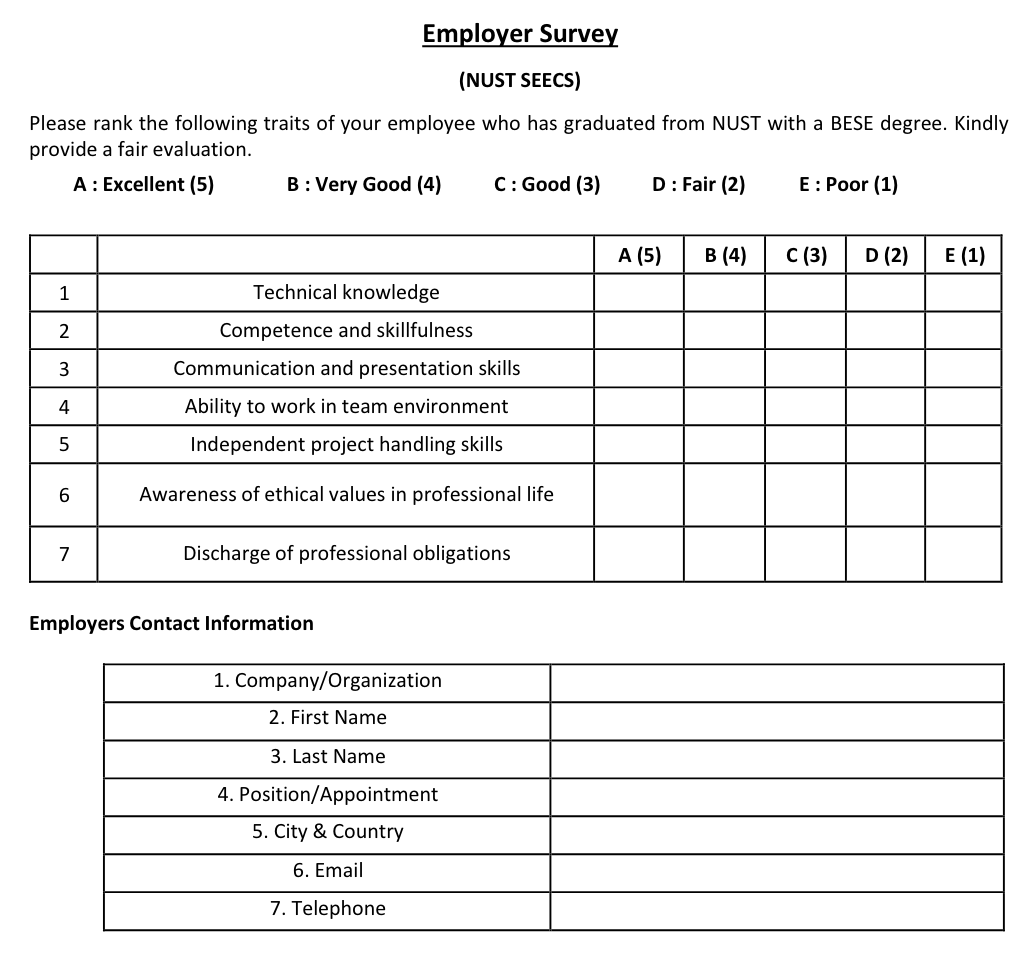
\includegraphics[width=1.0\textwidth]{images/front_matter/media/legacy employer form.png}}
\caption{Legacy Employer Survey Form}
\label{fig:legacy employer form}
\end{figure}

\begin{figure}[!h]
\centering
\fbox{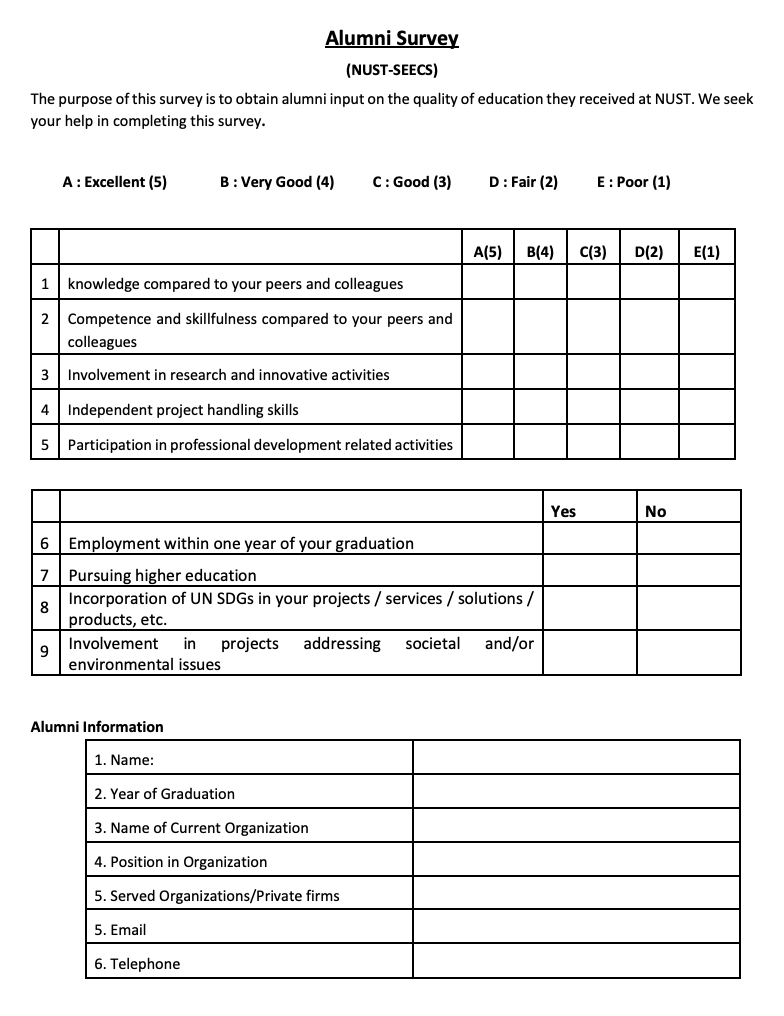
\includegraphics[width=1.0\textwidth]{appendices/criterion_1/legacy alumni form.png}}
\caption{Legacy Alumni Survey Form}
\label{fig:legacy alumni form}
\end{figure}

\section{Legacy PEO Evaluation System and Results (Pre-2026)}\label{app:legacy_peo_evaluation}

This annexure describes the evaluation mechanism and attainment results of the legacy PEO evaluation system, referenced in Criterion~1. 

\subsection{Legacy Evaluation Mechanism}

Under the legacy system, each PEO was assessed through a set of Key Performance Indicators (KPIs) derived from annual Alumni and Employer surveys. Indicator design accounted for diversity in graduate career paths e.g., employment, entrepreneurship, or higher education, so that a graduate's choice of path did not itself count against attainment. Each KPI was expressed as the percentage of respondents responding favourably to a specific survey item, with an attainment threshold of 50\% or 60\% depending on the indicator. A PEO was considered attained only if all of its constituent sub-KPIs individually met their respective thresholds, with cumulative PEO attainment computed as the equal-weight average of its sub-KPIs. Following KPIs were defined in the old scheme.

\noindent\textbf{PEO 1 --- Demonstrate sound software engineering knowledge and skill set.}
\begin{itemize}[leftmargin=1.5em,topsep=2pt]
\item 60\% of respondent employers are satisfied with technical knowledge of employed graduates.
\item 60\% of respondent employers are satisfied with competence and skills of employed graduates.
\item 60\% of respondent graduates gave positive feedback on their knowledge compared to their peers.
\item 60\% of respondent graduates gave positive feedback on their competence compared to their peers.
\item 50\% of respondent graduates are employed within one year of their graduation.
\item 50\% of respondent graduates are pursuing higher education.
\end{itemize}

\noindent\textbf{PEO 2 --- Lead diverse teams and work collaboratively to develop innovative solutions.}
\begin{itemize}[leftmargin=1.5em,topsep=2pt]
\item 60\% of respondent employers are satisfied with the communications skills of employed graduates.
\item 60\% of respondent employers are satisfied with the teamwork skills of employed graduates.
\item 60\% of respondent employers are satisfied with the independent project handling skills of employed graduates.
\item 60\% of respondent graduates are involved in research and/or innovation activities.
\item 60\% of respondent graduates have handled projects independently.
\item 50\% of respondent graduates are involved in professional development activities.
\end{itemize}

\noindent\textbf{PEO 3 --- Conduct professional practice for sustainable development with due consideration for societal, ethical, and environmental aspects.}
\begin{itemize}[leftmargin=1.5em,topsep=2pt]
\item 60\% of respondent employers are satisfied with adherence to ethical values by employed graduates.
\item 60\% of respondent employers are satisfied with the discharge of professional obligations of employed graduates.
\item 50\% of respondent graduates have incorporated UN SDGs in their projects / services / solutions / products etc.
\item 50\% of respondent graduates are involved in projects addressing societal and/or environmental issues.
\end{itemize}

\subsection{Legacy Evaluation Results (2025)}

Table~\ref{tab:legacy_results} presents the attainment results obtained under the legacy evaluation system, using Alumni and Employer survey data collected in 2025.
\setcounter{table}{0}
\renewcommand{\thetable}{A.\arabic{table}}
\begingroup
\scriptsize
\setlength{\tabcolsep}{4pt}
\renewcommand{\arraystretch}{1.2}
\begin{longtable}[]{@{}>{\raggedright\arraybackslash}p{0.06\textwidth}>{\raggedright\arraybackslash}p{0.52\textwidth}>{\raggedright\arraybackslash}p{0.20\textwidth}>{\centering\arraybackslash}p{0.10\textwidth}@{}}
\caption{Attainment of PEOs under the Legacy Evaluation System (Alumni/Employer surveys, data collected in 2025)}\label{tab:legacy_results}\\
\toprule
\multicolumn{4}{@{}>{\raggedright\arraybackslash}p{0.92\textwidth}@{}}{\textbf{PEO 1}: Demonstrate sound software engineering knowledge and skill set.}\\
\midrule
\textbf{S. No.} & \textbf{KPI} & \textbf{Measurement Tool} & \textbf{Attainment \%}\\
\midrule
\endfirsthead
\toprule
\textbf{S. No.} & \textbf{KPI} & \textbf{Measurement Tool} & \textbf{Attainment \%}\\
\midrule
\endhead
1 & 60\% of respondent employers are satisfied with technical knowledge of employed graduates & Employer Survey (Q1) & 85\%\\
2 & 60\% of respondent employers are satisfied with competence and skills of employed graduates & Employer Survey (Q2) & 86\%\\
3 & 60\% of respondent graduates gave positive feedback on their knowledge compared to their peers & Alumni Survey (Q1) & 76\%\\
4 & 60\% of respondent graduates gave positive feedback on their competence compared to their peers & Alumni Survey (Q2) & 76\%\\
5 & 50\% of respondent graduates are employed within one year of their graduation & Alumni Survey (Q6) & 89\%\\
6 & 50\% of respondent graduates are pursuing higher education & Alumni Survey (Q7) & 36\%\\
\addlinespace
\midrule
\multicolumn{4}{@{}>{\raggedright\arraybackslash}p{0.92\textwidth}@{}}{\textbf{PEO 2}: Lead diverse teams and work collaboratively to develop innovative solutions.}\\
\midrule
\textbf{S. No.} & \textbf{KPI} & \textbf{Measurement Tool} & \textbf{Attainment \%}\\
\midrule
1 & 60\% of respondent employers are satisfied with the communications skills of employed graduates & Employer Survey (Q3) & 84\%\\
2 & 60\% of respondent employers are satisfied with the teamwork skills of employed graduates. & Employer Survey (Q4) & 85\%\\
3 & 60\% of respondent employers are satisfied with the independent project handling skills of employed graduates & Employer Survey (Q5) & 81\%\\
4 & 60\% of respondent graduates are involved in research and/or innovation activities & Alumni Survey (Q3) & 69\%\\
5 & 60\% of respondent graduates have handled projects independently & Alumni Survey (Q4) & 79\%\\
6 & 50\% of respondent graduates are involved in professional development activities & Alumni Survey (Q5) & 76\%\\
\addlinespace
\midrule
\multicolumn{4}{@{}>{\raggedright\arraybackslash}p{0.92\textwidth}@{}}{\textbf{PEO 3}: Conduct professional practice for sustainable development with due consideration for societal, ethical, and environmental aspects.}\\
\midrule
\textbf{S. No.} & \textbf{KPI} & \textbf{Measurement Tool} & \textbf{Attainment \%}\\
\midrule
1 & 60\% of respondent employers are satisfied with adherence to ethical values by employed graduates. & Employer Survey (Q6) & 86\%\\
2 & 60\% of respondent employers are satisfied with the discharge of professional obligations of employed graduates. & Employer Survey (Q7) & 78\%\\
3 & 50\% of respondent graduates have incorporated UN SDGs in their projects / services / solutions / products etc. & Alumni Survey (Q8) & 52\%\\
4 & 50\% of respondent graduates are involved in projects addressing societal and/or environmental issues. & Alumni Survey (Q9) & 64\%\\
\bottomrule
\end{longtable}
\endgroup

Under the legacy criterion requiring every sub-KPI to meet its threshold individually, PEO~2 and PEO~3 were fully attained. For PEO~1, five of the six sub-KPIs exceeded their thresholds. The indicator measuring the proportion of graduates pursuing higher education reached 36\% against a 50\% threshold. On an equal-weight cumulative basis, the attainment levels were approximately 75\%, 79\%, and 70\% for PEO~1, PEO~2, and PEO~3, respectively. 

Figure~\ref{fig:legacy_analysis} shows the per-KPI attainment for each PEO under the legacy evaluation system, with the dashed line in each panel indicating the applicable attainment threshold (50\% or 60\%, depending on the indicator). All indicators meet their respective thresholds except PEO~1 KPI-6 (pursuing higher education), which falls below its 50\% threshold.

\begin{figure}[tb]
\centering
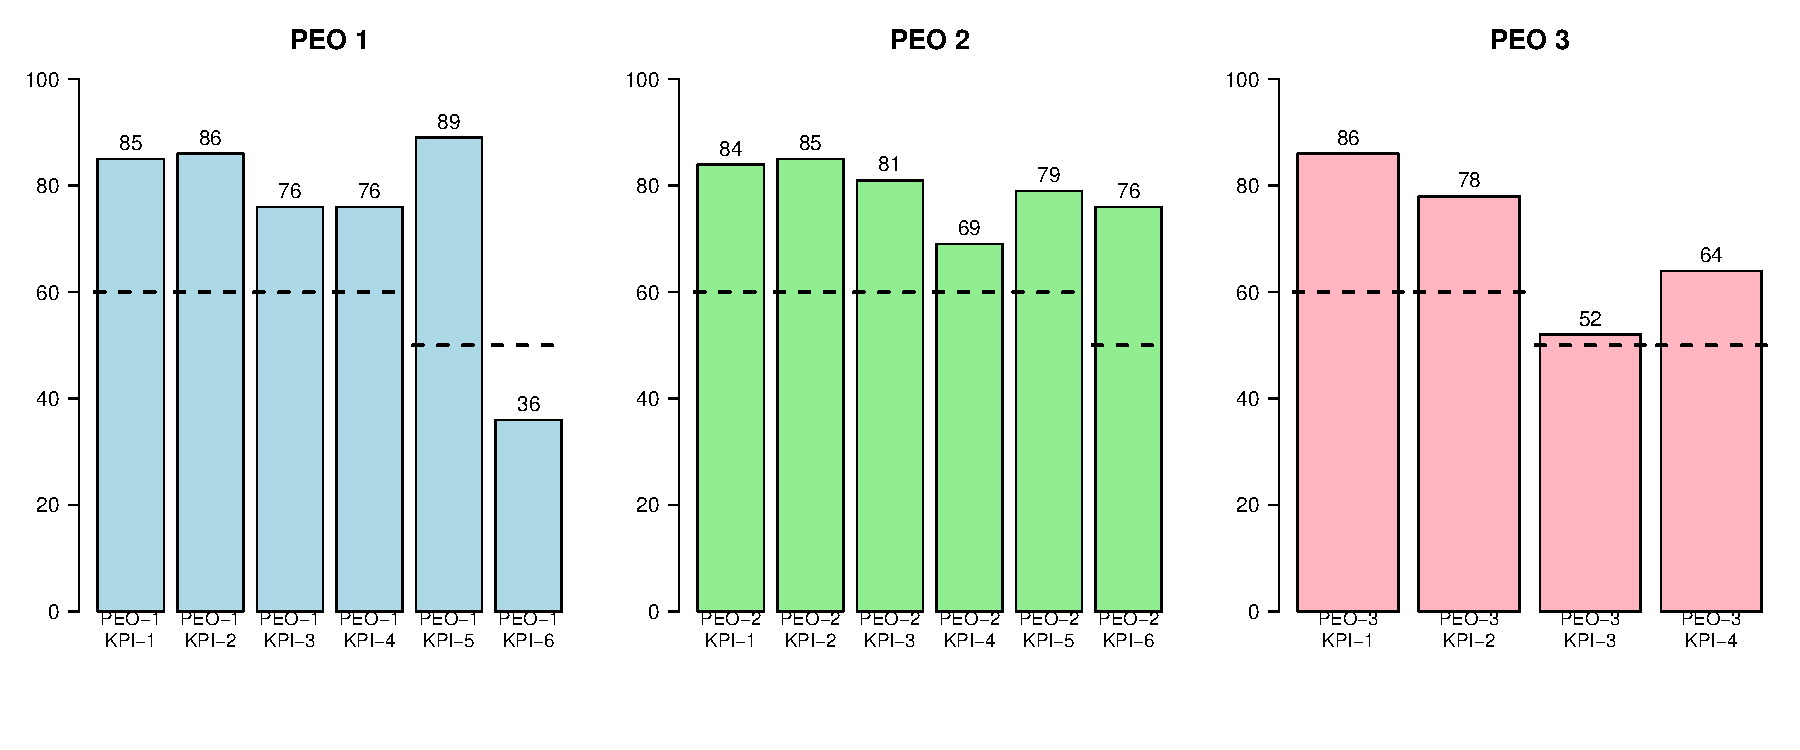
\includegraphics[width=\textwidth]{images/criterion_1/media/legacy_analysis.pdf}
\caption{Per-KPI attainment under the Legacy Evaluation System (data collected in 2025). The dashed line in each panel marks the applicable attainment threshold for that indicator.}
\label{fig:legacy_analysis}
\end{figure}

The single below-threshold indicator reflects a structural limitation of the legacy instrument rather than a shortfall in program outcomes. Pursuit of higher education is a binary indicator that does not, on its own, represent PEO attainment, since graduates who enter employment instead of higher education are not demonstrating a deficiency against the objective. Limitations of this nature where indicators are only loosely aligned with PEO-level outcomes, together with a rigid all-or-nothing pass rule, motivated the revised evaluation system described in Criterion~1.

\section{IAB Feedback: Full Closed-Loop and Open Recommendation Records}\label{app:iab_feedback_full}

This annexure reproduces, in full, the two IAB feedback tables summarized in Criterion~1. The complete closed-loop record of feedback items with documented evidence of implementation, and the complete list of standing/open recommendations, restricted to items sourced from IAB sessions held in 2024 or later, with one exception, i.e. the 13th November 2023 session is retained below because it is the documented origin of the Revised (2026) PEO Evaluation System, the report's principal CQI action (Section~\ref{attainment-of-peos}). The official minutes underlying these entries, including the 13th November 2023 session, are reproduced in Appendix~\ref{app:iab_minutes} and evidence folder.

\subsection{Closed-Loop Actions: Feedback Implemented and Verified (Full Record)}

\begingroup
\footnotesize
\setlength{\tabcolsep}{4pt}
\renewcommand{\arraystretch}{1.2}
\begin{longtable}[]{@{}>{\raggedright\arraybackslash}p{0.28\textwidth}>{\raggedright\arraybackslash}p{0.18\textwidth}>{\raggedright\arraybackslash}p{0.46\textwidth}@{}}
\caption{Closed-Loop IAB Feedback and Actions Taken (2023 origin item retained, otherwise 2025)}\label{tab:iab_closed_loop}\\
\toprule
\textbf{Industry Feedback} & \textbf{Source / Date} & \textbf{Action Taken}\\
\midrule
\endfirsthead
\toprule
\textbf{Industry Feedback} & \textbf{Source / Date} & \textbf{Action Taken}\\
\midrule
\endhead
\midrule
\multicolumn{3}{r}{\footnotesize\itshape Continued on next page}\\
\endfoot
\bottomrule
\endlastfoot
Alumni Survey item (Q5) was found to inadequately assess PEO-2 attainment. & IAB Meeting, 13th November 2023 & As recorded in the minutes (ref:Detailed minutes evidence folder ), the item was relocated to PEO-3, where it aligns with the corresponding KPI, endorsed in the same session.\\
\addlinespace
PEC observation (2023 Accreditation Visit): Lack of correlation in the survey forms used to assess certain PEO-2/PEO-3 sub-KPIs, reinforced by the IAB's concern over Alumni Survey Q5 (see above). & PEC Accreditation Visit, 2023, reiterated IAB Meeting, 13th November 2023 & The Alumni and Employer Survey instruments were fully redesigned, with items mapped directly to PEOs, as the Revised (2026) Evaluation System. The revised forms were reviewed and approved by the SE Departmental Board of Studies (DBS) on 20th April 2026. These were presented to and ratified by the SEECS HoDs' forum and the Faculty Board of Studies (FBS) of 21st April 2026, and finally presented to and endorsed by the IAB on 5th May 2026. The approved forms were then circulated by email to Alumni and Employers for input and used at the department's Open House in May 2026.\\
\addlinespace
Introduce a Quantum Computing course. & IAB Meeting, 28th February 2025 (CEO, Emumba) & A dedicated elective, ``Introduction to Quantum Computing'' (offered in 3+1 and 2+1 credit-hour variants, covering superposition, entanglement, quantum algorithms, and hands-on labs using Qiskit-based simulators), was proposed via a SEECS-wide working paper (sponsored by SEECS, not the SE department alone) for inclusion as an elective in the BESE (Software Engineering), BSCS, BSAI, and BSDS curricula. The working paper records the course as approved by the DBS, for introduction from Spring 2026.\\
\addlinespace
Enable cross-departmental minor courses (e.g., SEECS students taking courses at NBS). & IAB Meeting, 28th February 2025 & Already available under NUST's University-wide Minors policy: SEECS students including (Software Engineering) may register for the Management minor at NUST Business School (NBS), subject to a minimum CGPA of 2.75, while SEECS reciprocally offers minors in Software Engineering, Computer Science, Data Science, and Artificial Intelligence to students of other NUST institutions (NUST Undergraduate Student Handbook, 28th August 2024 edition, Chapter 6, Para 2 ``Option of Minors'').\footnote{National University of Sciences and Technology, \textit{Undergraduate Student Handbook}, 28th August 2024 edition, Chapter 6, Para 2. Available at \url{https://seecs.nust.edu.pk/wp-content/uploads/2024/09/28-Aug-2024-Undergraduate-Handbook.pdf}.}\\
\addlinespace
Consider open-book examination formats. & IAB Meeting, 28th February 2025 (ITnIS Consulting) & Already available under existing NUST examination policy: the concerned faculty/invigilator may announce, in advance of a quiz, OHT, or mid/end-semester examination, the books, notes, or other material students may refer to during the test, effectively enabling an open-book format at faculty discretion (NUST Undergraduate Student Handbook, 28th August 2024 edition, Chapter 2, Para 8 ``Use of Reference Material during Test/Examination'').\footnote{National University of Sciences and Technology, \textit{Undergraduate Student Handbook}, 28th August 2024 edition, Chapter 2, Para 8. Available at \url{https://seecs.nust.edu.pk/wp-content/uploads/2024/09/28-Aug-2024-Undergraduate-Handbook.pdf}.}\\
%\addlinespace
%Introduce certification-style courses. & IAB Meeting, 28th February 2025 (ITnIS Consulting) & NUST recently approved 1–3 CH range (per WP No. 2, 73rd ACM, 9th February 2026, in consistence with HEC's CS/IT-specific elective-replacement provision (Letter HEC/CURR/GEN/2025/8036, 15th September 2025, Annex-A, Para 5), but differs from PEC's own proposal of a broader 6–12 CH range floated at its Task Force's inaugural meeting of 21st May 2025 and subsequently circulated for institutional input via Letter PEC/EAD/EQEEP/2025/04 (14th July 2025). That proposal remains subject to ratification by PEC's Engineering Accreditation Board (EAB) and Governing Body and has not yet been issued as a final SOP. The department intends to therefore adopt NUST policy in line with the more specific and more recent HEC guidance while awaiting PEC's final mechanism, and will revise credit-hour equivalencies if required once PEC's SOP is issued.\\
\end{longtable}
\endgroup

\subsection{Standing and Emerging Recommendations (Full Record)}

\begingroup
\footnotesize
\setlength{\tabcolsep}{4pt}
\renewcommand{\arraystretch}{1.2}
\begin{longtable}[]{@{}>{\raggedright\arraybackslash}p{0.68\textwidth}>{\raggedright\arraybackslash}p{0.24\textwidth}@{}}
\caption{Open IAB Recommendations Pending Implementation}\label{tab:iab_open}\\
\toprule
\textbf{Recommendation (Not Yet Closed)} & \textbf{Source / Date}\\
\midrule
\endfirsthead
\toprule
\textbf{Recommendation (Not Yet Closed)} & \textbf{Source / Date}\\
\midrule
\endhead
\midrule
\multicolumn{2}{r}{\footnotesize\itshape Continued on next page}\\
\endfoot
\bottomrule
\endlastfoot
Expand coverage of AI agents, reverse engineering, and data-science algorithms. & IAB Meeting, 28th February 2025 (CEO, Emumba)\\
Establish a faculty ``boot camp'' to close the skills gap between academia and industry practice, targeted at PhD/MS scholars. & IAB Meeting, 7th May 2025, recorded as Action Point 2\\
Broaden ``Applied AI in Education'' into a cross-sector applied-AI offering. Split DevOps and Machine Learning into separate courses. & IAB Meeting, 7th May 2025, recorded as Action Point 1\\
Formalise a mentorship partnership (e.g., with Novatec X) to provide affordable, industry-led mentorship to students and researchers. & IAB Meeting, 7th May 2025, recorded as Action Point 3\\
Improve student and faculty access to premium cloud/AI tools to maximise use of available cloud-credit programmes. & IAB Meeting, 7th May 2025, recorded as Action Point 4\\
Increase the number of internship placements and recruitment drives connected to Open House events. & IAB Meeting, 28th February 2025\\
Continue to strengthen graduate soft skills, communication, customer orientation, and professional ethics, a recurring, sustained industry request across multiple sessions. & IAB Meetings: 2nd May 2024, 28th February 2025, 5th May 2026\\
\end{longtable}
\endgroup
%%%%%%%%%%%%%%%%%%%%%%%%%%%%%%%%%%%

\section{IAB Meeting Minutes (2023 Origin Session, and 2024--2026)}\label{app:iab_minutes}

The original minutes of the selected few relevent Industry Advisory Board (IAB) sessions cited in Criterion~1 are reproduced below exactly as recorded. Details of each IAB proceeding with each session presented will be provided in evidence folder at the time of visit.

\begin{figure}[!h]
\centering
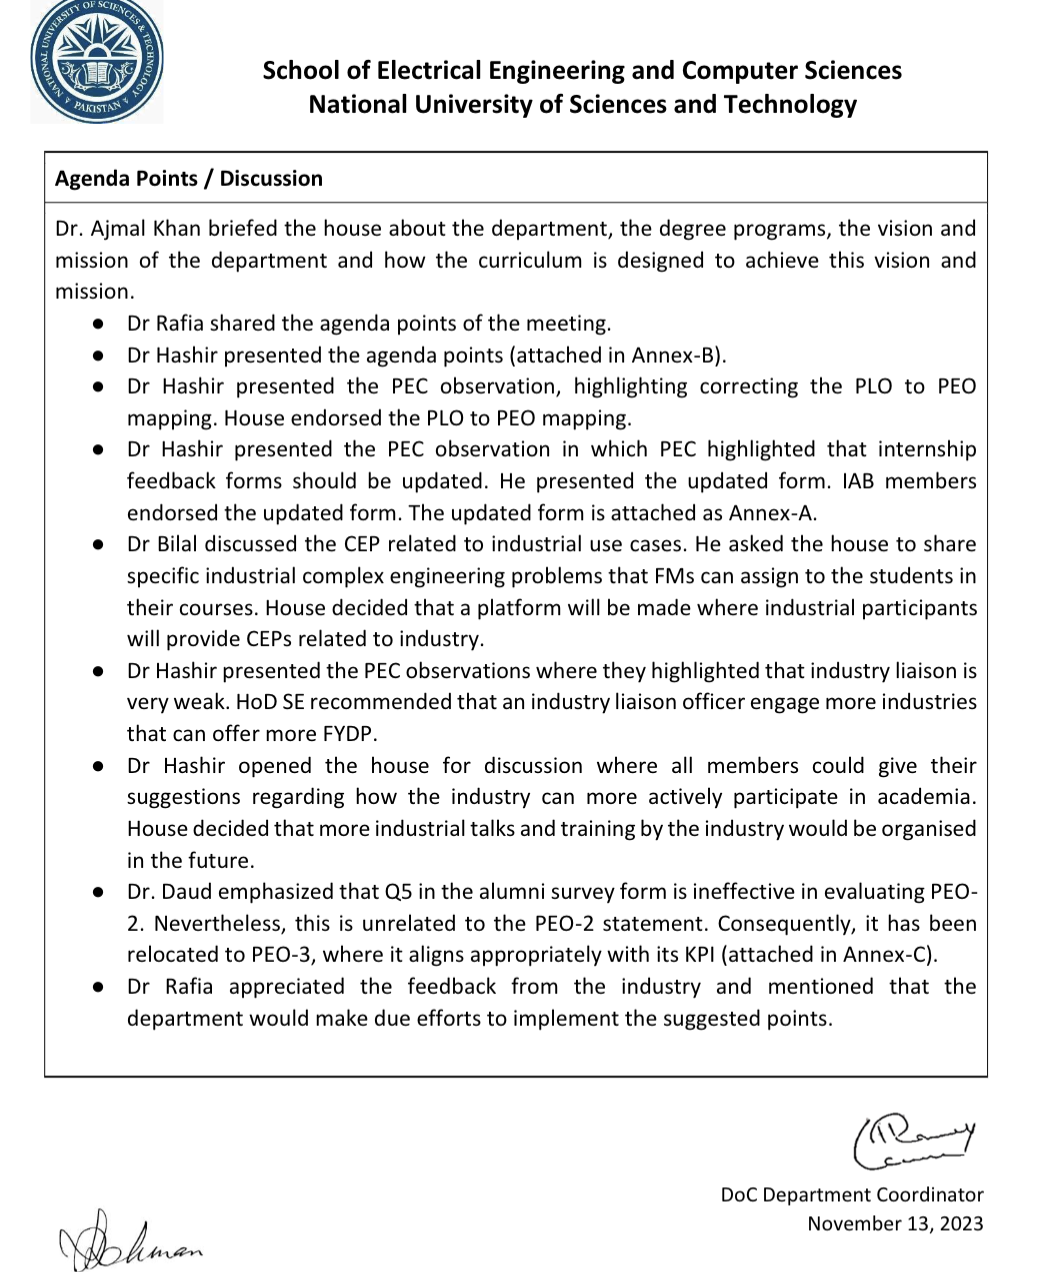
\includegraphics[width=0.8\textwidth]{appendices/criterion_1/IAB 2023.png}
\caption{IAB Meeting Minutes 13th November 2023}
\label{fig:iab 2023}
\end{figure}

The meeting on 13th November 2023 was attended by following faculty and industry representatives.

\begin{figure}[!h]
\centering
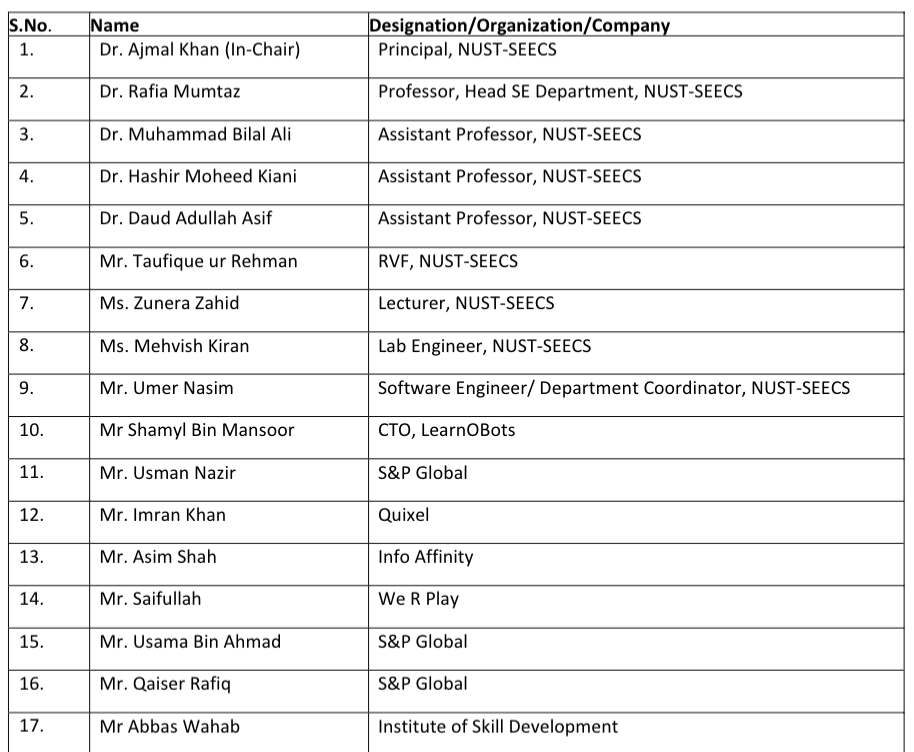
\includegraphics[width=0.79\textwidth]{appendices/criterion_1/iab 2023 attendance.png}
\caption{IAB Meeting Participants 13th November 2023}
\label{fig:iab 2023 attendees}
\end{figure}

The subsequent IAB meeting was held on 2nd May 2024. 

\begin{figure}[!h]
\centering

\includegraphics[width=0.79\textwidth]{appendices/criterion_1/iab 2024a.png}
\caption{IAB Meeting 2nd May 2024}
\label{fig:iab 2024a}
\end{figure}

\begin{figure}[!h]
\centering
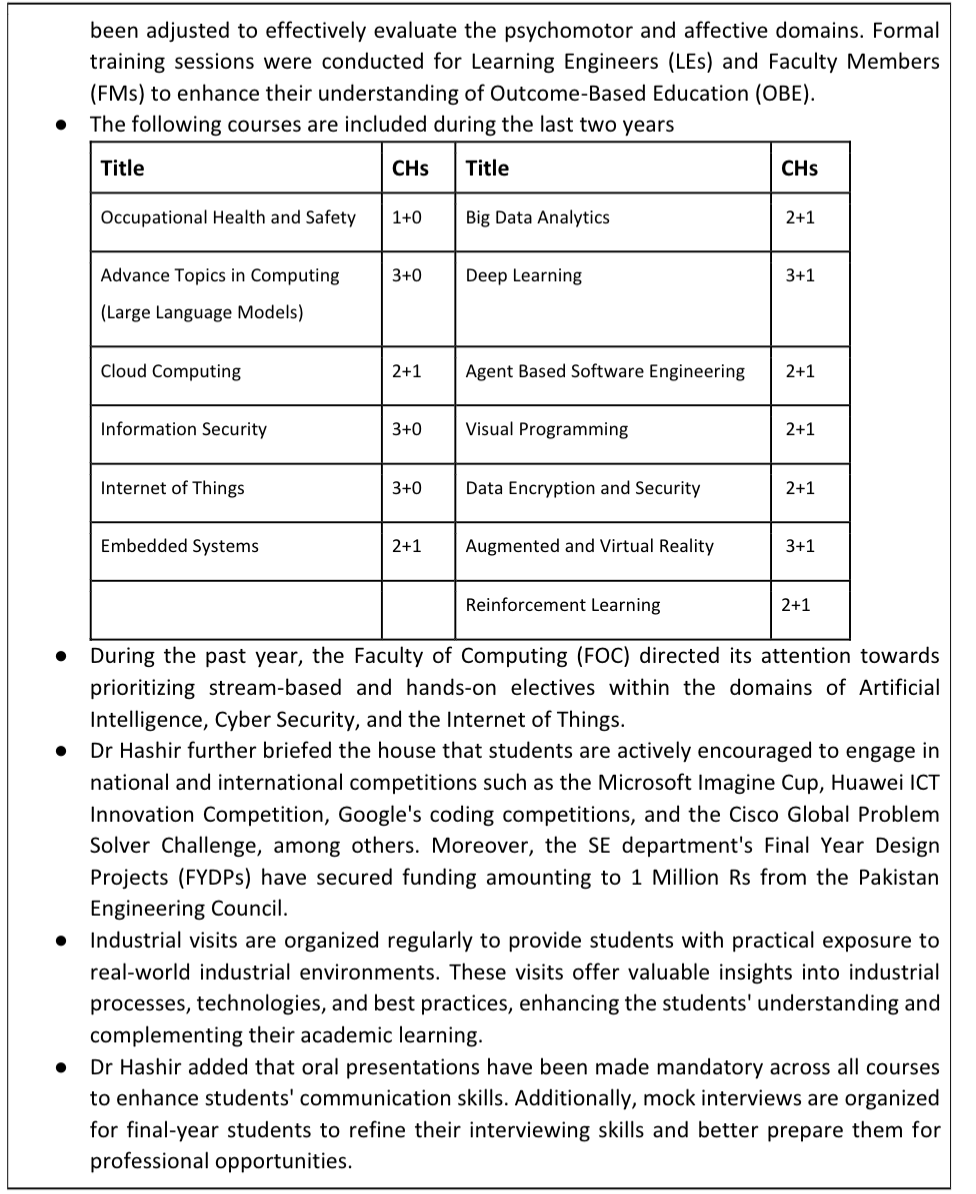
\includegraphics[width=0.85\textwidth]{appendices/criterion_1/iab 2024b.png}
\caption{IAB Meeting 2nd May 2024}
\label{fig:iab 2024b}
\end{figure}

Major participants included:

\begin{figure}[!h]
\centering
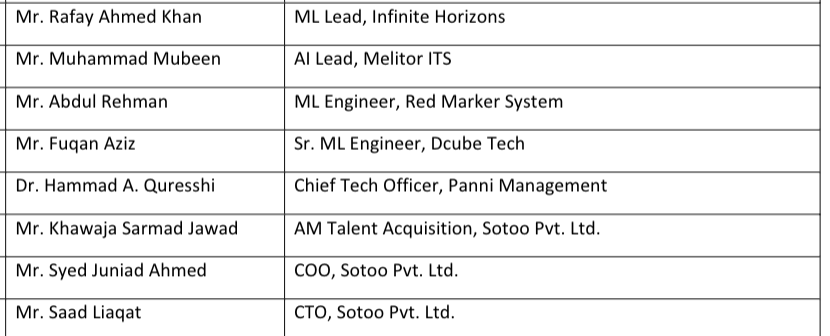
\includegraphics[width=0.75\textwidth]{appendices/criterion_1/iab 2024 attendees.png}
\caption{IAB Meeting Participants 2nd May 2024}
\label{fig:iab 2024 part}
\end{figure}

The next IAB meeting was held on 28th February 2025.

\begin{figure}[!h]
\centering
\fbox{
\includegraphics[width=0.80\textwidth]{appendices/criterion_1/iab 2025a.png}}
\caption{IAB Meeting 28th February 2025}
\label{fig:iab 2025a}
\end{figure}

\begin{figure}[!h]
\centering
\fbox{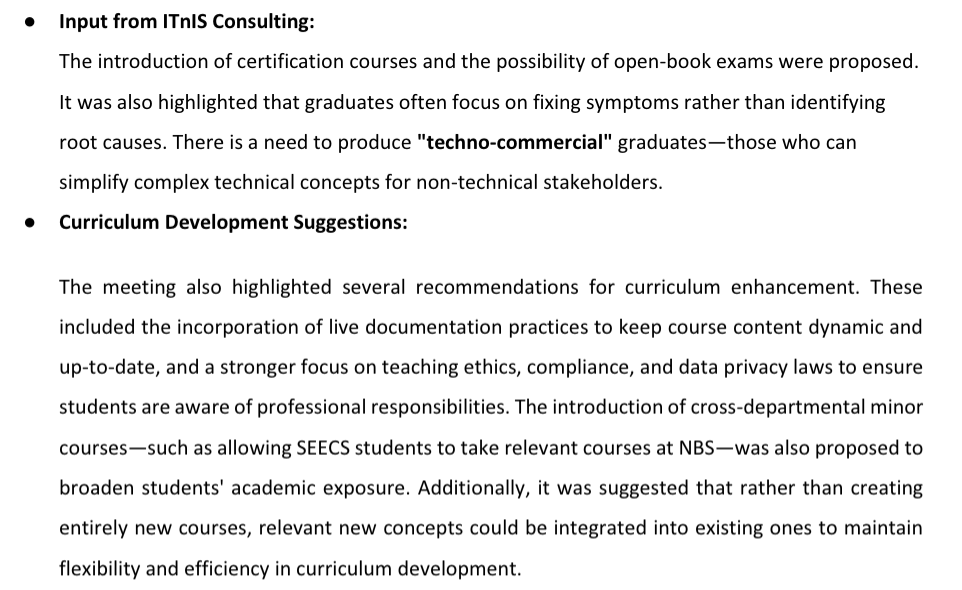
\includegraphics[width=0.80\textwidth]{appendices/criterion_1/iab 2025b.png}}
\caption{IAB Meeting 28th February 2025}
\label{fig:iab 2025b}
\end{figure}

The list of participants of the meeting is presented below:
\begin{figure}[!h]
\centering
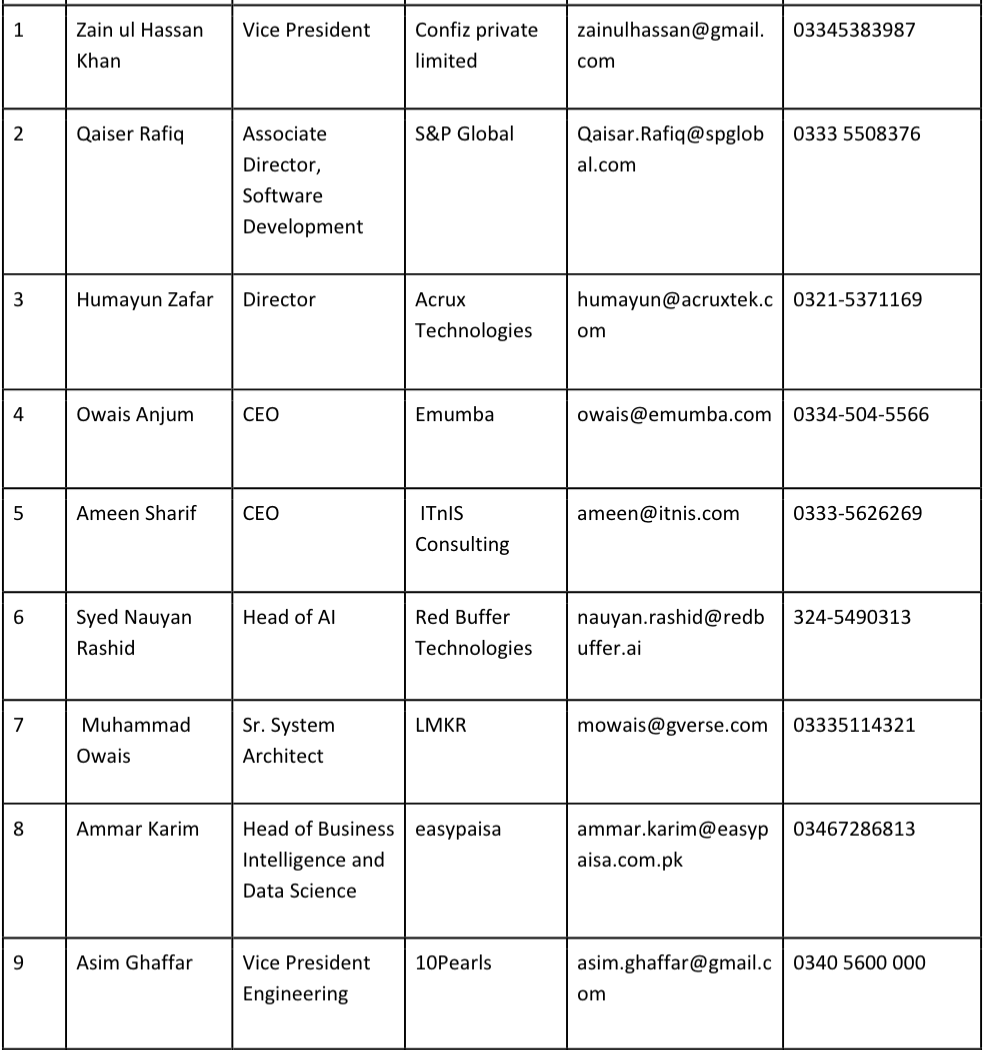
\includegraphics[width=0.75\textwidth]{appendices/criterion_1/iab 2025 attendees.png}
\caption{IAB Meeting Participants 28th February 2025}
\label{fig:iab 2025 attendees}
\end{figure}

The subsequent IAB meeting was held on 7th May 2025.

\begin{figure}[!h]
\centering
\fbox{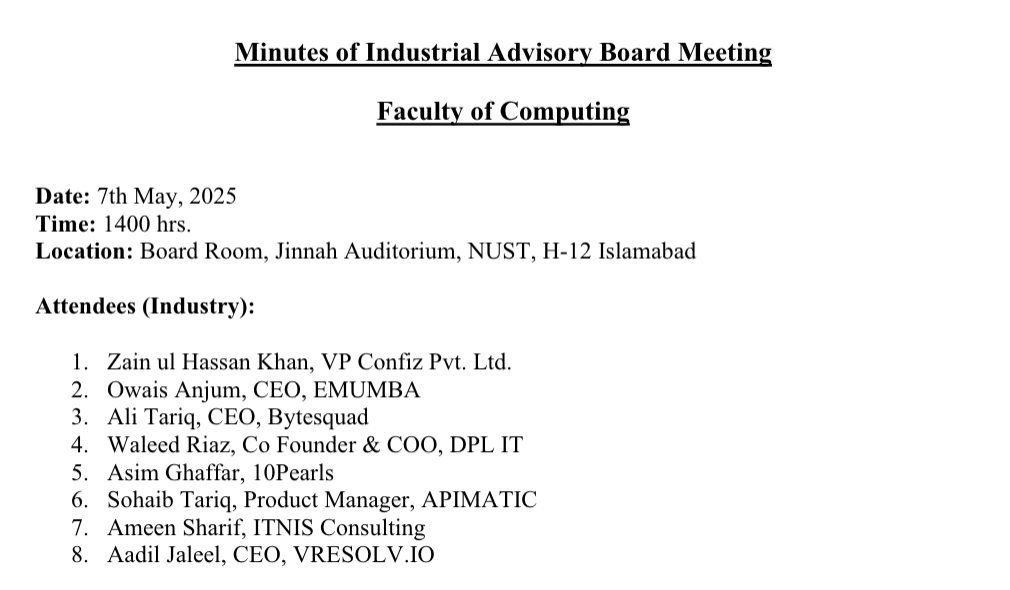
\includegraphics[width=0.80\textwidth]{appendices/criterion_1/iab 2025c.png}}
\caption{IAB Meeting Participants 7th May 2025}
\label{fig:iab 2025-2 attendees}
\end{figure}

\begin{figure}[!h]
\centering
\fbox{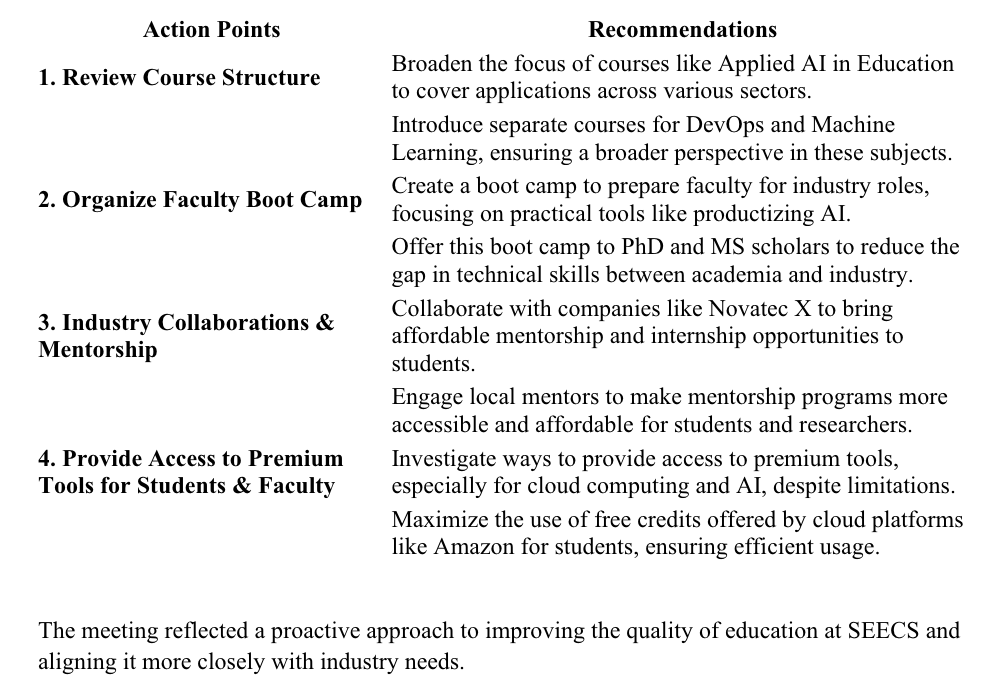
\includegraphics[width=0.85\textwidth]{appendices/criterion_1/iab 2025d.png}}
\caption{IAB Meeting 7th May 2025}
\label{fig:iab 2025d}
\end{figure}

The latest IAB meeting was held on 5th May 2026. The meeting was attended by following industry representatives:

\begin{figure}[!h]
\centering
\fbox{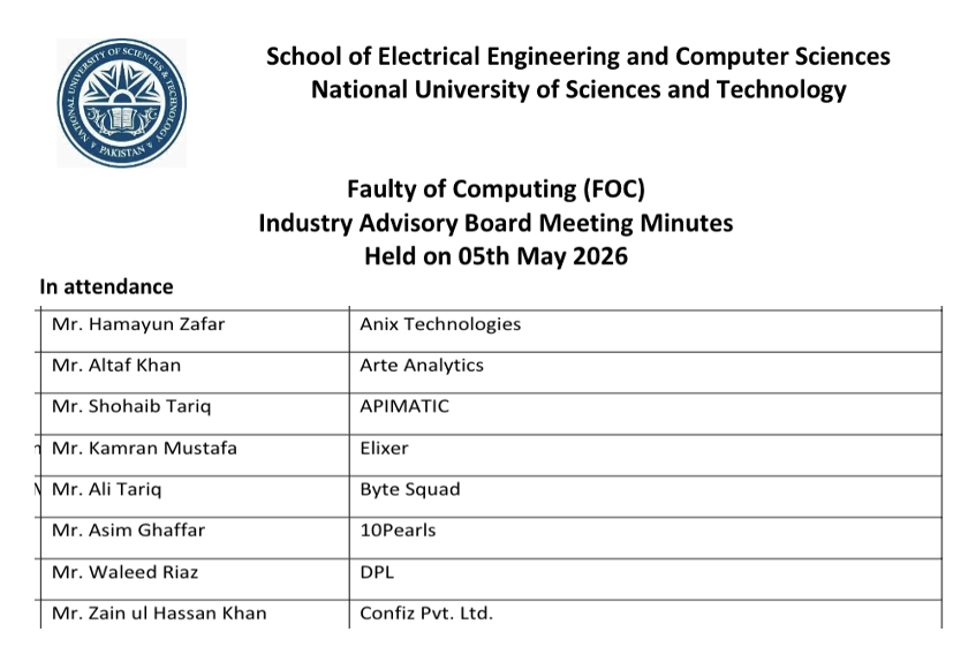
\includegraphics[width=0.85\textwidth]{appendices/criterion_1/iab 2026 attendees.png}}
\caption{IAB Meeting Participants 5th May 2026}
\label{fig:iab 2026 attendees}
\end{figure}

The main agenda points discussed in the meeting were following:

\begin{figure}[!ht]
\centering
\fbox{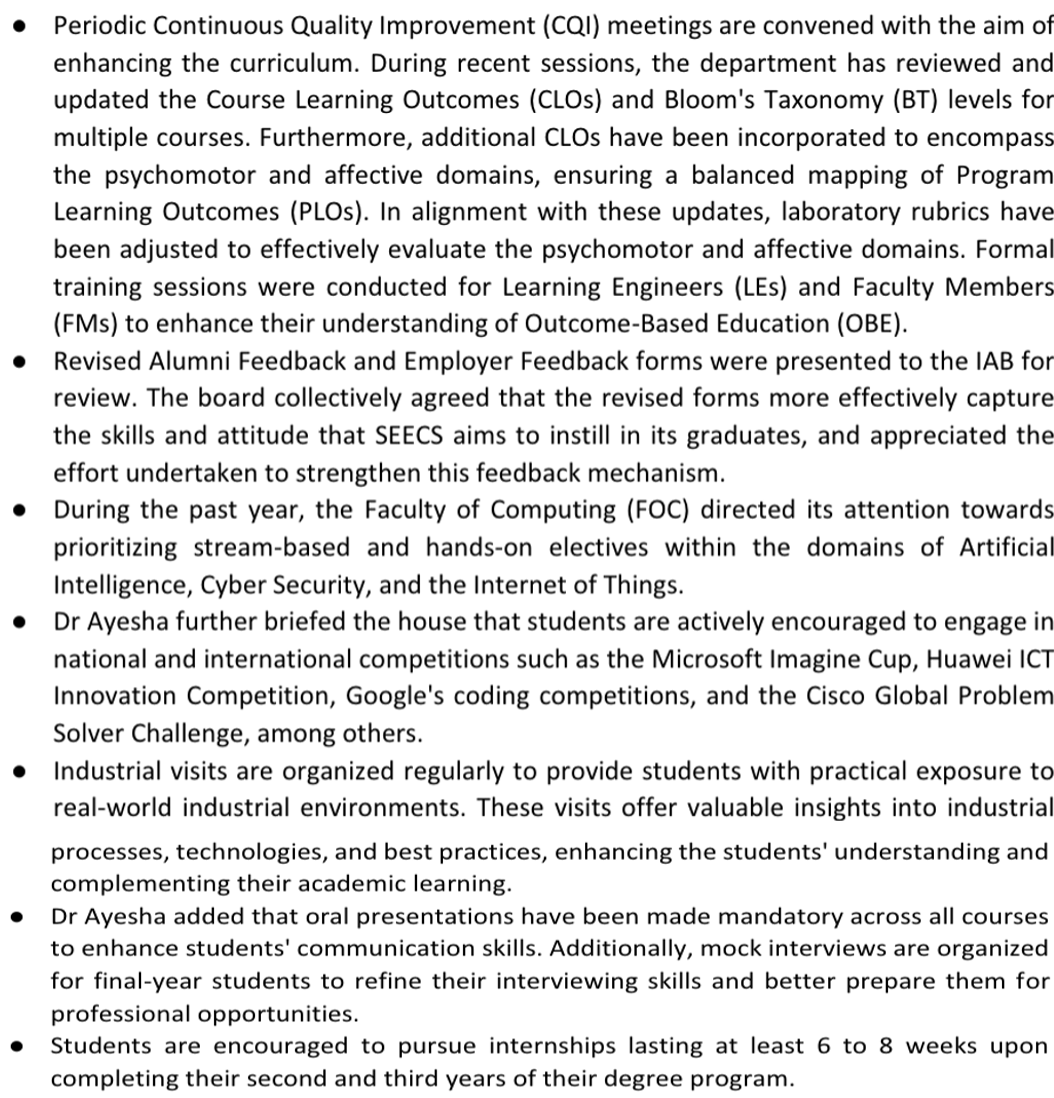
\includegraphics[width=0.85\textwidth]{appendices/criterion_1/iab 2026a.png}}
\caption{IAB Meeting 5th May 2026}
\label{fig:iab 2026a}
\end{figure}

\begin{figure}[!hb]
\centering
\fbox{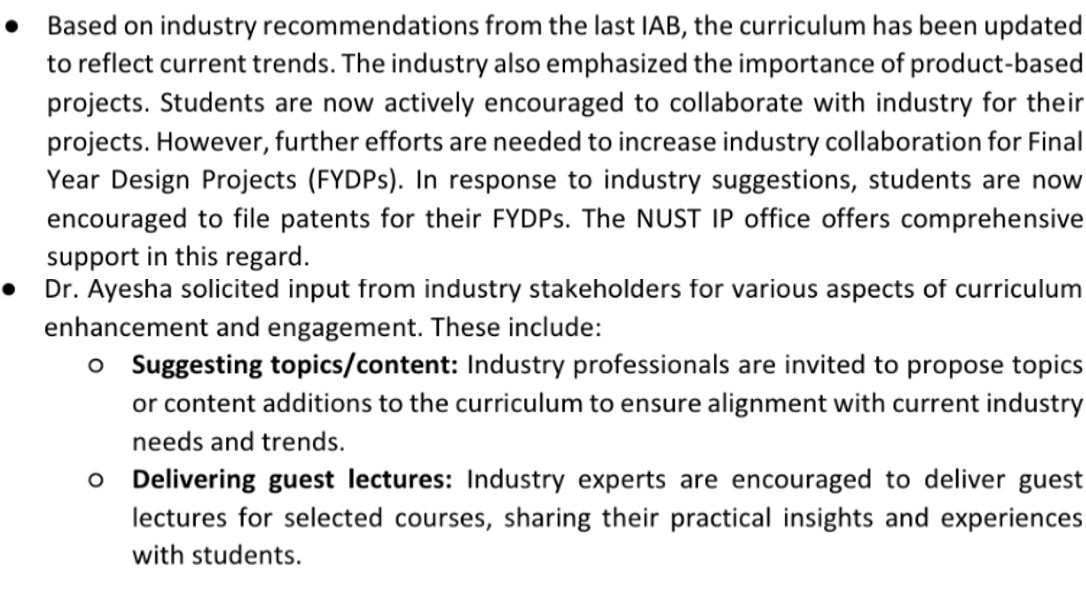
\includegraphics[width=0.85\textwidth]{appendices/criterion_1/iab 2026b1.png}}
\caption{IAB Meeting 5th May 2026}
\label{fig:iab 2026b1}
\end{figure}

\begin{figure}[!h]
\centering
\fbox{
\includegraphics[width=0.90\textwidth]{appendices/criterion_1/iab 2026c.png}}
\caption{IAB Meeting 5th May 2026}
\label{fig:iab 2026c}
\end{figure}

%Section~\ref{app:iab_feedback_full}. The 13th November 2023 session is retained below as the documented origin of the Revised (2026) PEO Evaluation System (Section~\ref{attainment-of-peos}).

%\subsection{IAB Meeting, 13th November 2023}
%The source file for this session also contains an appended briefing presentation (Annex-B) and PEO/KPI slides (Annex-C); consistent with the minutes-and-attendees-only scope of this section, only the two-page minutes and attendee list are reproduced below.
%\IfFileExists{appendices/criterion_1/IAB Meeting minutes - 13th Nov 2023.pdf}{%
%\begin{center}
%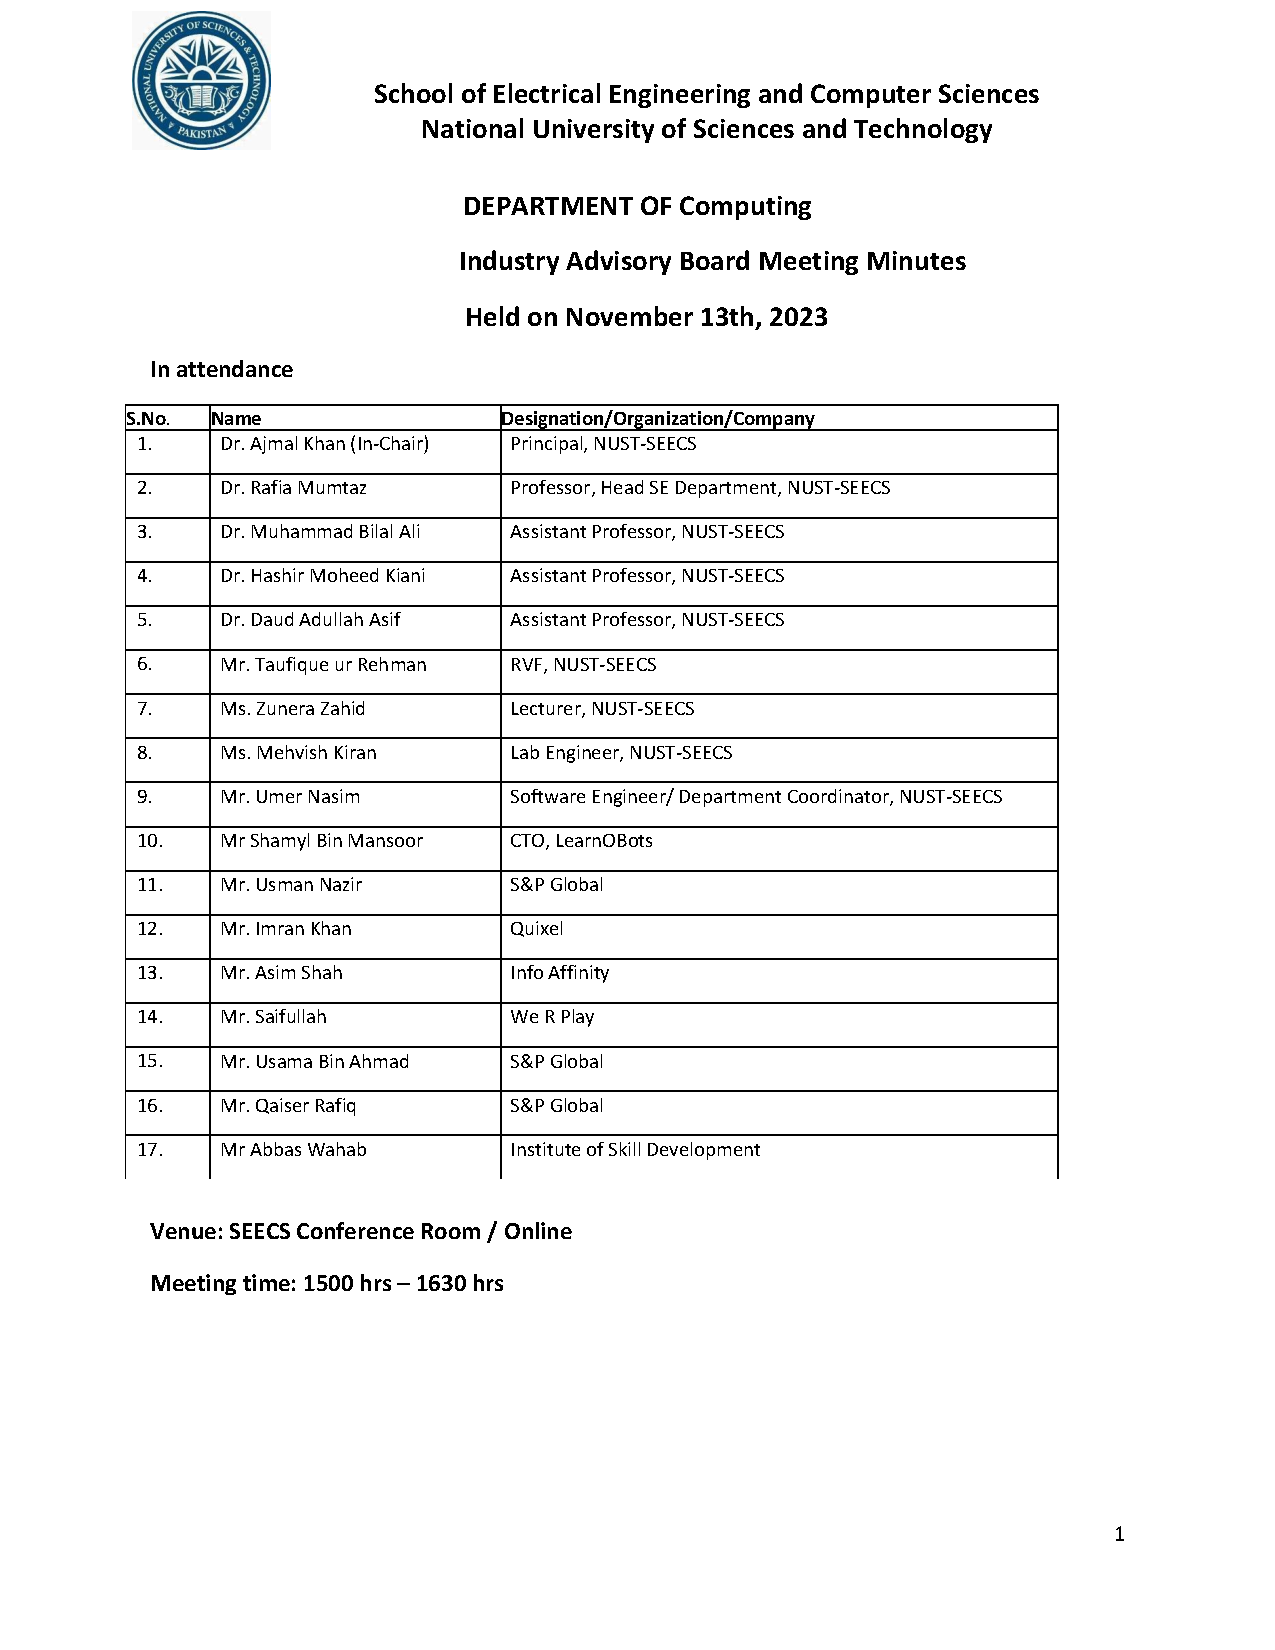
\includegraphics[page=1,width=0.92\textwidth]{appendices/criterion_1/IAB Meeting minutes - 13th Nov 2023.pdf}
%\end{center}
%\includepdf[pages=2]{appendices/criterion_1/IAB Meeting minutes - 13th Nov 2023.pdf}%
%}{\missingannexure{appendices/criterion_1/IAB Meeting minutes - 13th Nov 2023.pdf}}

%\subsection{IAB Meeting, 2nd May 2024}
%\includeminutesannexure{appendices/criterion_1/IAB Meeting minutes - 02nd May 2024.pdf}

%\subsection{IAB Meeting, 28th February 2025}
%\includeminutesannexure{appendices/criterion_1/IAB Meeting Minutes 28th Feb 2025.pdf}

%\subsection{IAB Meeting, 7th May 2025}
%\includeminutesannexure{appendices/criterion_1/IAB Meeting minutes 7th May 2025.pdf}

%\subsection{IAB Meeting, 5th May 2026}
%\includeminutesannexure{appendices/criterion_1/IAB_Meeting_minutes_05th_May_2026.pdf}

\section{Governance Minutes and Policy Documents }\label{app:governance_minutes}

This annexure presents the governance minutes and supporting policy documents cited in Criterion~1. Together, they provide documentary evidence that the Software Engineering programme operates within a formal, multi-level governance structure in which proposals are reviewed, approved and escalated through the appropriate academic bodies, and that stakeholder feedback is systematically acted upon. The annexure comprises the following documents:
\begin{itemize}
  \item Departmental Board of Studies (DBS) minutes, 20th April 2026.
  \item Faculty Board of Studies (FBS) minutes, 21st April 2026.
  \item Revised Internship Assessment Policy.
\end{itemize}

\begin{figure}[!h]
\centering
\fbox{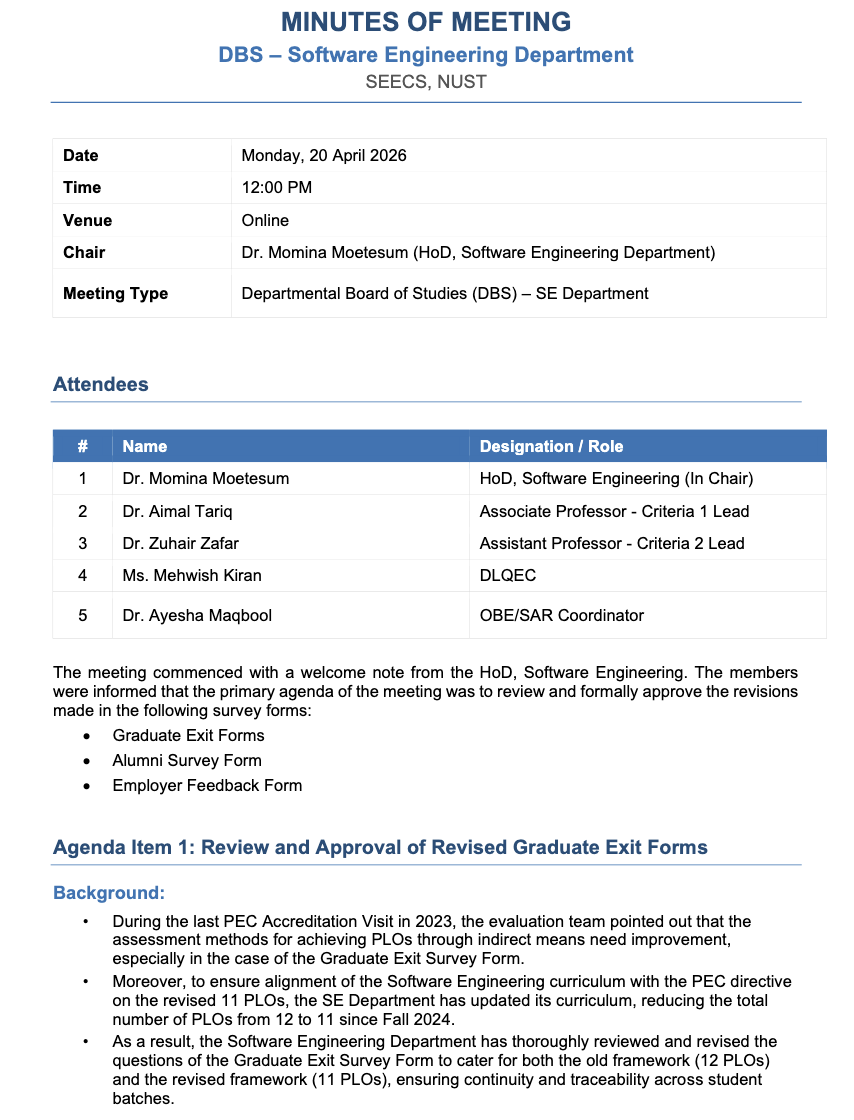
\includegraphics[width=1.0\textwidth]{appendices/criterion_1/dbs1.png}}
\caption{Department Board of Studies Meeting 20th April 2026}
\label{fig:dbs1}
\end{figure}

\begin{figure}[!h]
\centering
\fbox{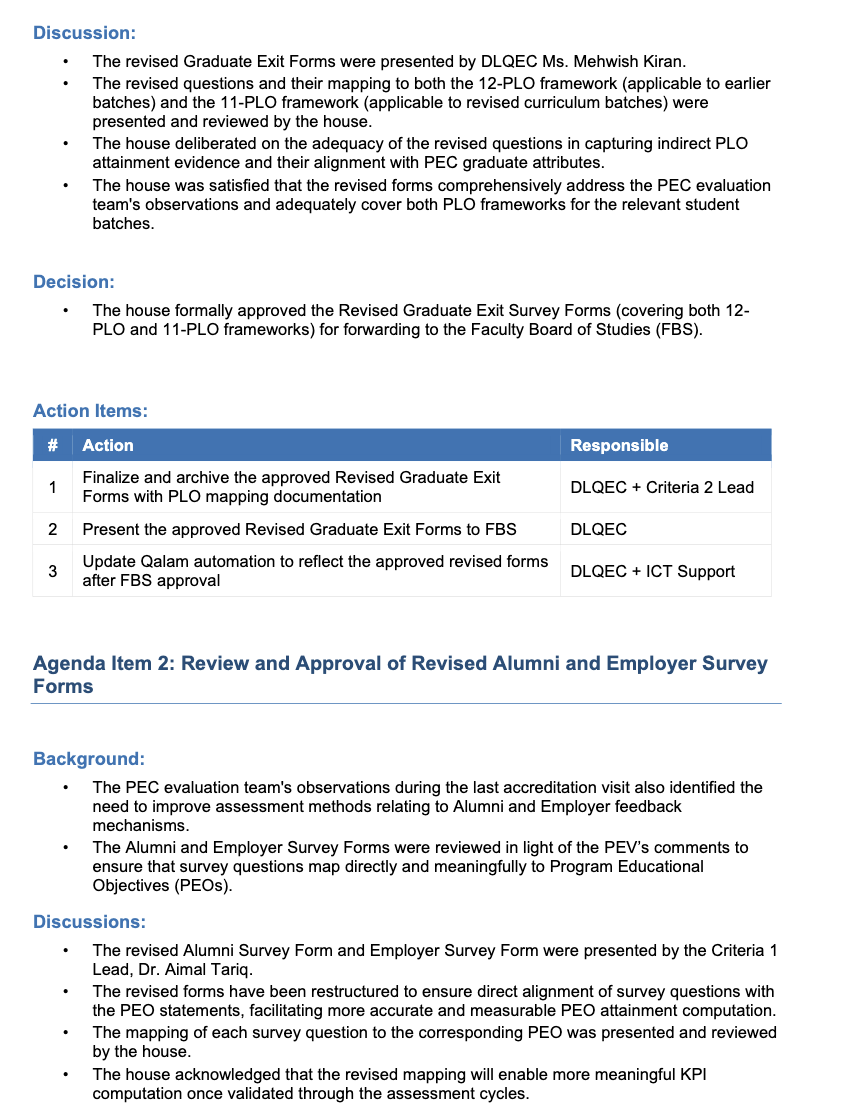
\includegraphics[width=1.0\textwidth]{appendices/criterion_1/dbs2.png}}
\caption{Department Board of Studies Meeting 20th April 2026}
\label{fig:dbs2}
\end{figure}

In addition, the DBS-approved working paper for the new elective course ``Introduction to Quantum Computing'', together with the proposal for the minor in Software Engineering, will be presented in detail in the
supporting evidence folder.

\begin{figure}[!h]
\centering
\fbox{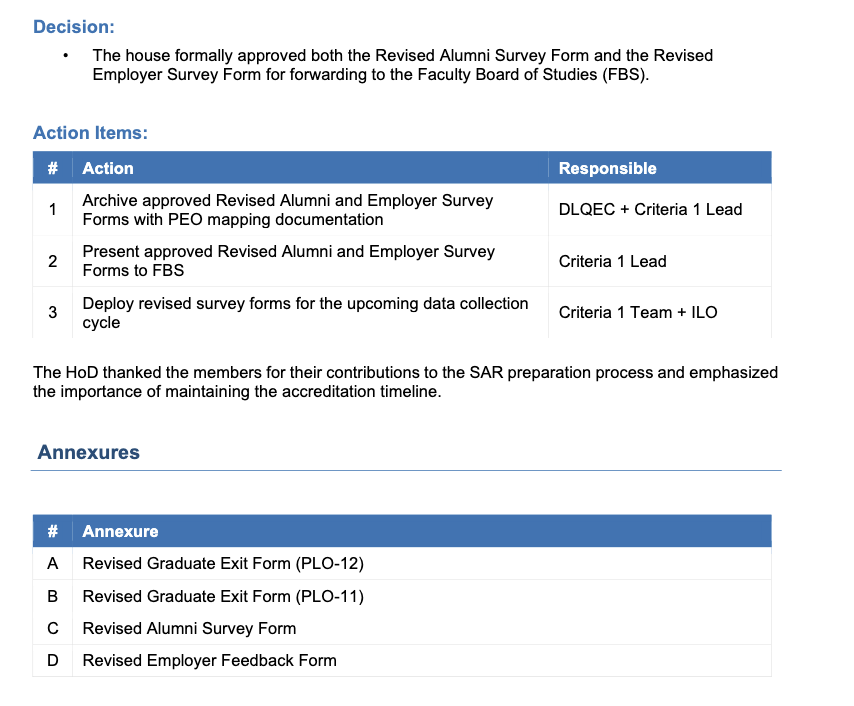
\includegraphics[width=0.75\textwidth]{appendices/criterion_1/dbs3.png}}
\caption{Department Board of Studies Meeting 20th April 2026}
\label{fig:dbs3}
\end{figure}

\begin{figure}[!h]
\centering
\fbox{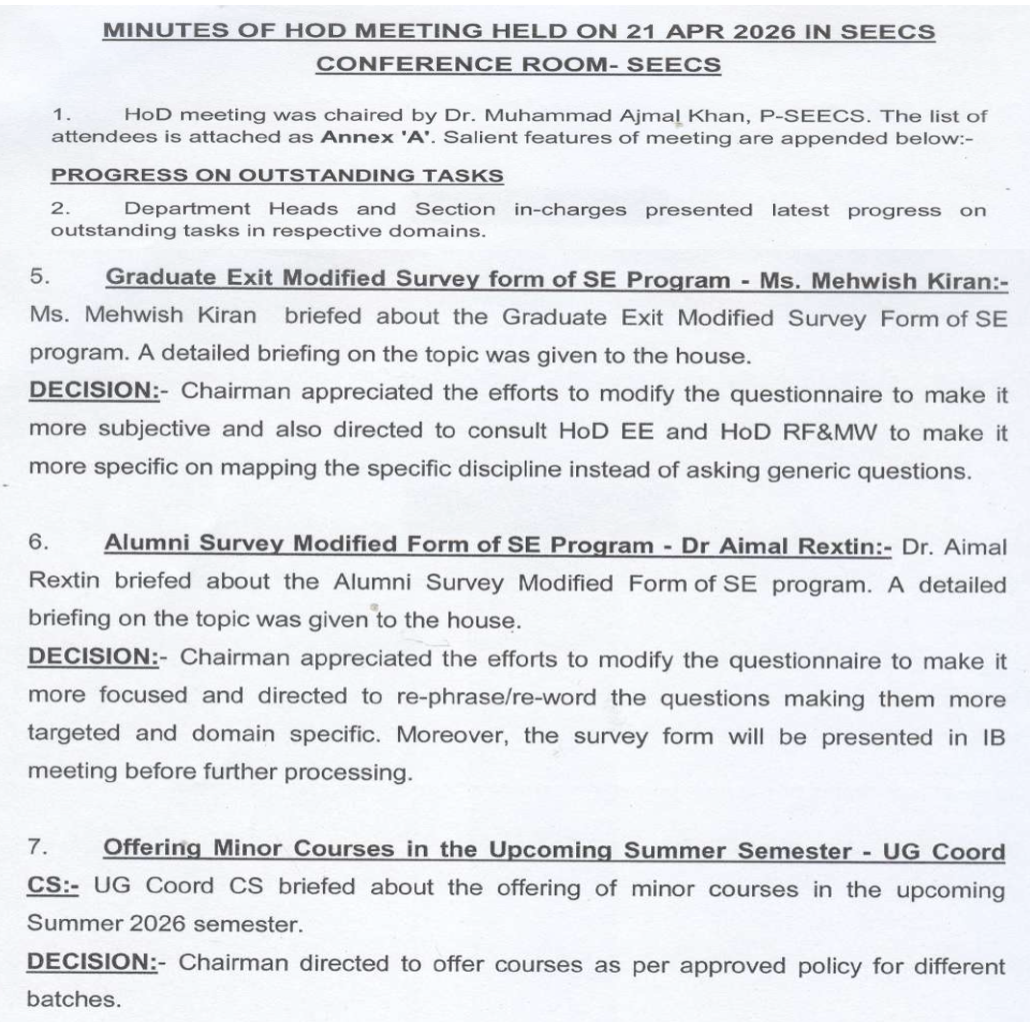
\includegraphics[width=0.75\textwidth]{appendices/criterion_1/fbs1.png}}
\caption{Faculty Board of Studies Meeting 21th April 2026}
\label{fig:fbs1}
\end{figure}

\begin{figure}[!h]
\centering
\fbox{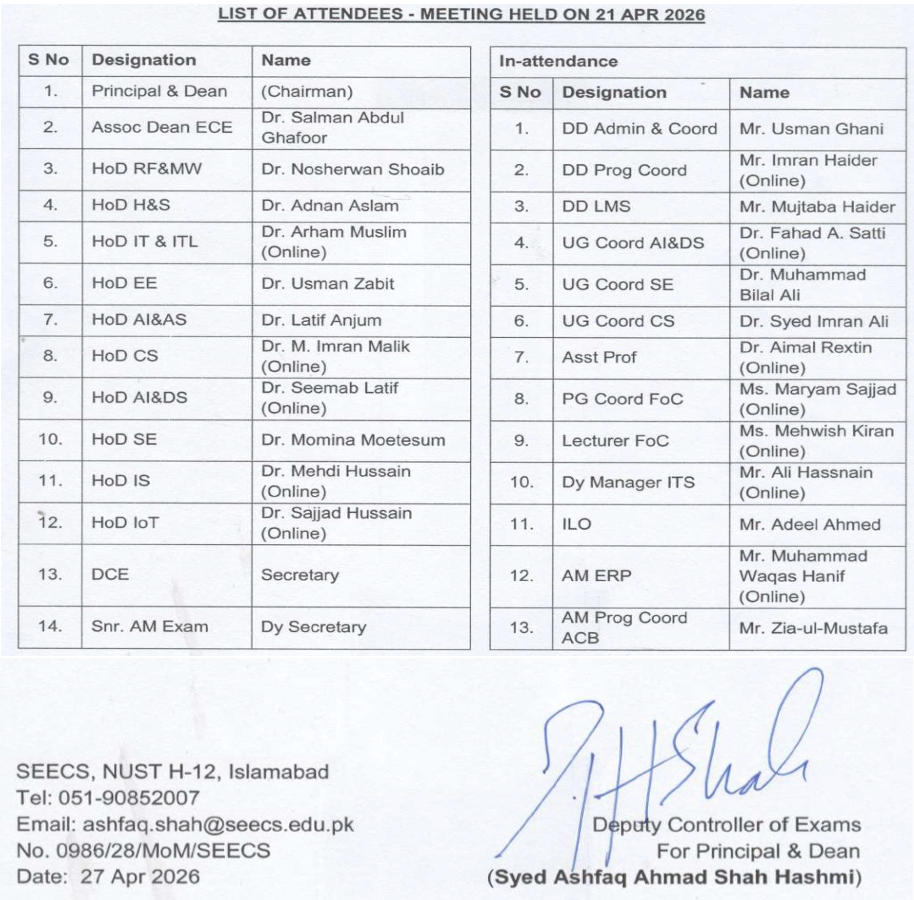
\includegraphics[width=0.80\textwidth]{appendices/criterion_1/fbs2.png}}
\caption{Faculty Board of Studies Meeting 20th April 2026}
\label{fig:fbs2}
\end{figure}

The internship policy defines the roles and responsibilities of the parties involved,
namely the student, the departmental internship supervisor and the industry supervisor at the host organisation. It specifies how student performance is evaluated, including the evaluation criteria, the weightage given to the industry supervisor's assessment and to the student's internship report, and the requirements for submitting documents. 
\begin{figure}[!h]
\centering
\fbox{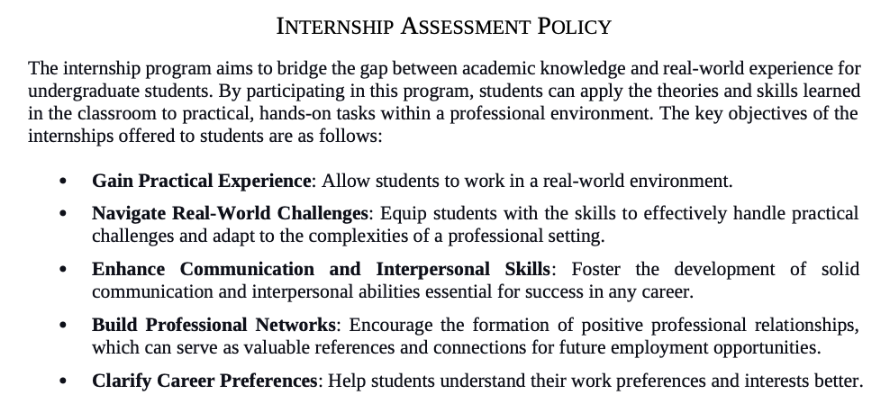
\includegraphics[width=0.80\textwidth]{appendices/criterion_1/internship1.png}}
\caption{Revised Internship Assessment Policy}
\label{fig:intern1}
\end{figure}

\begin{figure}[!h]
\centering
\fbox{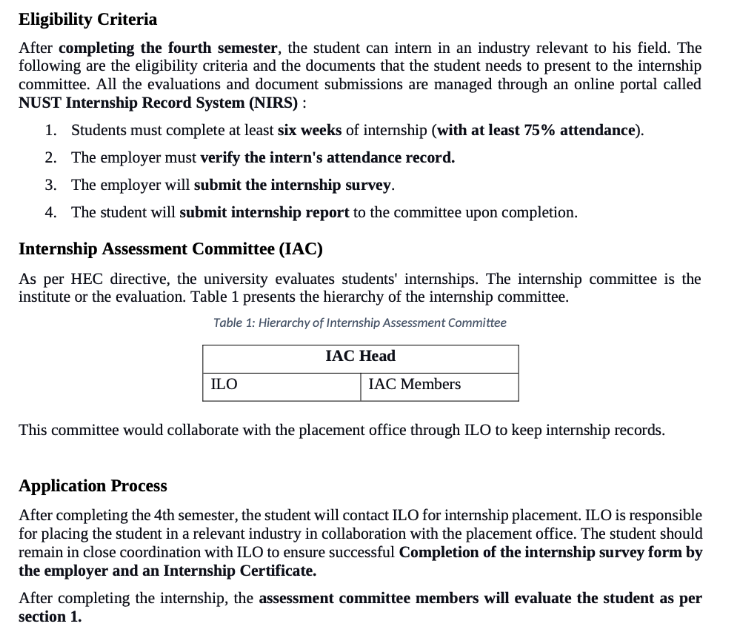
\includegraphics[width=0.80\textwidth]{appendices/criterion_1/internship1b.png}}
\caption{Revised Internship Assessment Policy}
\label{fig:intern1b}
\end{figure}

\begin{figure}[!h]
\centering
\fbox{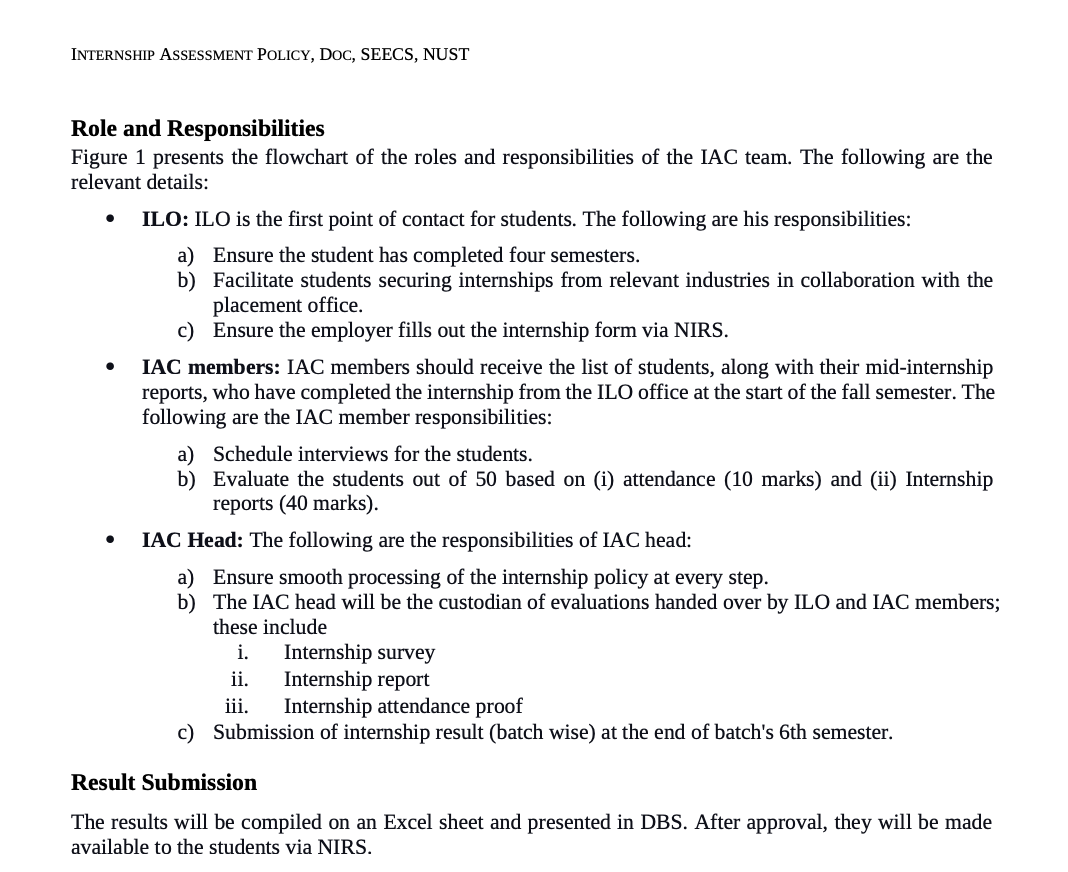
\includegraphics[width=0.80\textwidth]{appendices/criterion_1/internship2.png}}
\caption{Revised Internship Assesssment Policy}
\label{fig:intern2}
\end{figure}

\begin{figure}[!h]
\centering
\fbox{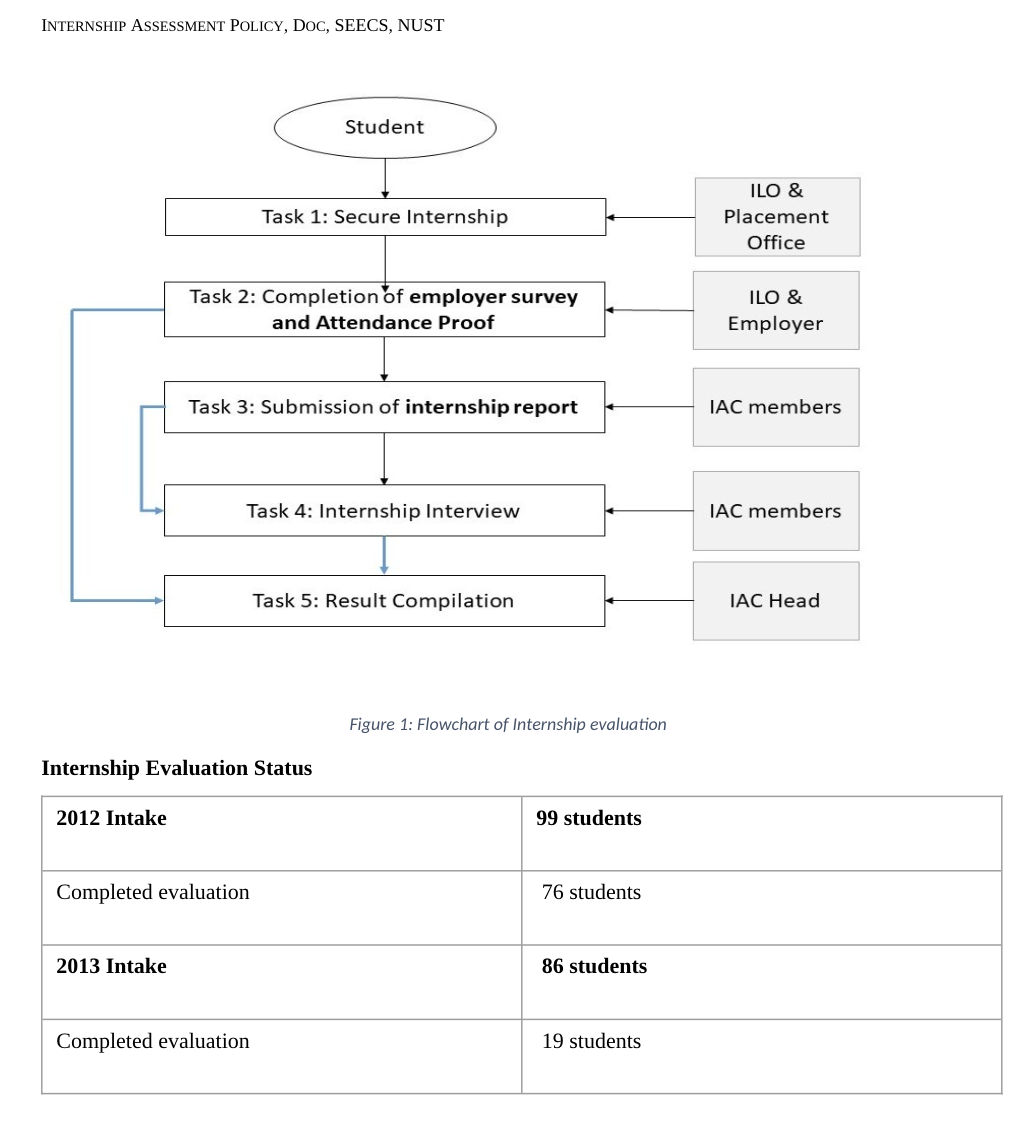
\includegraphics[width=0.80\textwidth]{appendices/criterion_1/internship3.png}}
\caption{Revised Internship Assessment Policy}
\label{fig:intern3}
\end{figure}

%\subsection{Internship Assessment Policy}
%\includefullannexure{appendices/criterion_1/Internship_Assessment_Procedure.pdf}

%\subsection{Minor in Software Engineering Offering in Spring 2026}
%\includefullannexure{appendices/criterion_1/Minors.pdf}

%%%%%%%%%%%%%%%%%%%%%%%%%%%%%%%%%%%
\newpage
\section{Revised Survey Forms}\label{app:revised forms}
The full Alumni and Employer Survey forms referenced in Criterion~1 are reproduced below exactly as administered, covering the revised (2026) evaluation system. These two instruments constitute the primary tools for the
indirect assessment of the Programme Educational Objectives (PEOs). The Alumni Survey captures graduates' views on how well the programme has prepared them
for their careers and continued professional growth, while the Employer Survey records the perspective of organisations that employ or supervise our
graduates on their technical competence, professional conduct and overall performance in the workplace.

\begin{figure}[!h]
\centering
\fbox{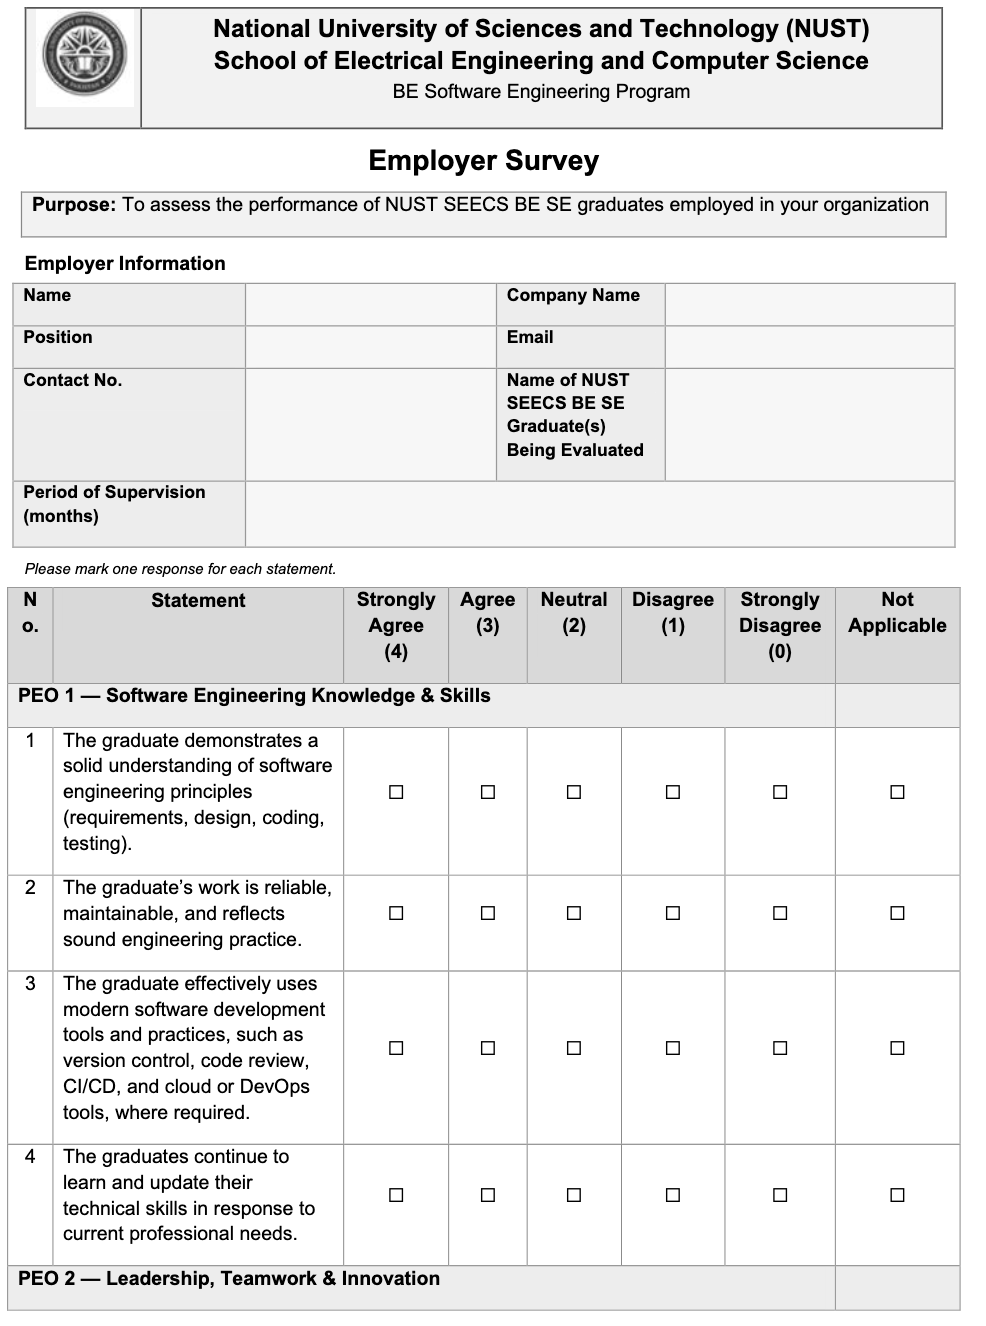
\includegraphics[width=1.0\textwidth]{appendices/criterion_1/revised employer form.png}}
\caption{Revised Employer Survey Form}
\label{fig:revised employer form}
\end{figure}

\begin{figure}[!h]
\centering
\fbox{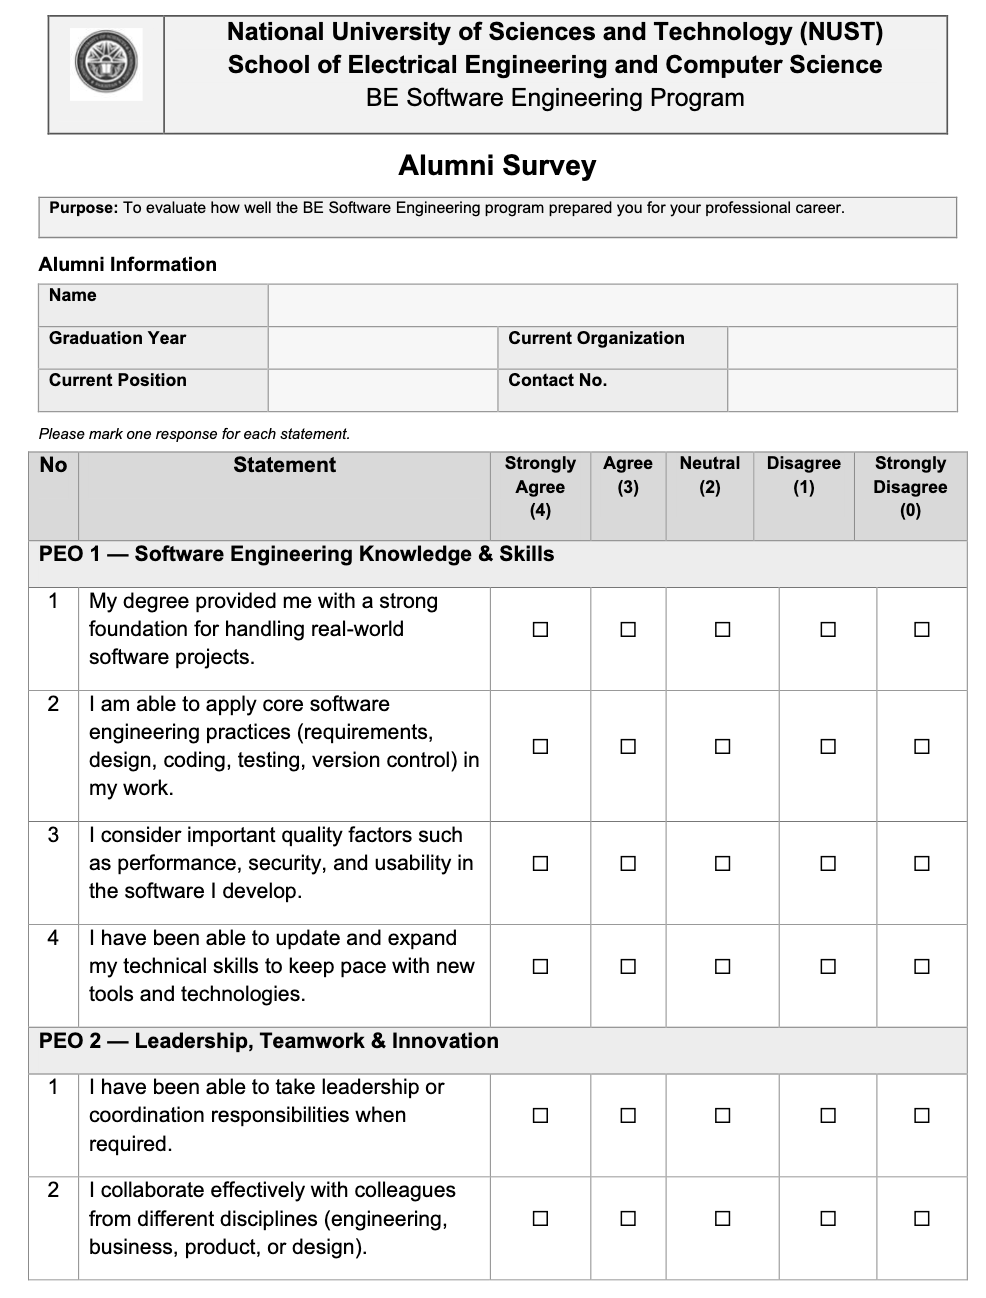
\includegraphics[width=1.0\textwidth]{appendices/criterion_1/revised alumni form.png}}
\caption{Revised Alumni Survey Form}
\label{fig:revised alumni form}
\end{figure}





%%%%%%%%%%%%%%%%%%%%%%%%%%%%%%%%%
%\section{Incorporation of Certifications in Degree Program}\label{app:certifications}

%This appendix highlights current directives from various governing bodies regarding inclusion/incorporation of certifications in degree programs. The Pakistan Engineering Council (PEC) (Letter PEC/EAD/EQEEP/2025/04, 14th July 2025)asked for institutional input on integrating international certifications into engineering programs in lieu of 6–12 credit hours of elective coursework. The Higher Education Commission (HEC) (Letter HEC/CURR/GEN/2025/8036, 15th September 2025) subsequently issued a formal advisory mandating incorporation of industry certifications and internships into undergraduate programs, with specific provision for CS/IT programs to replace electives with certifications equivalent to 3 credit hours. In response, NUST processed Working Paper No. 2 (73rd ACM, 9th February 2026), endorsed at UCAP on 30th January 2026, establishing a formal mechanism for certification credit-hour recognition (1–3 CH per certification, subject to CLO-mapping, department-level validation/assessment, and ACM approval), recommended for implementation with immediate effect. Each directive is presented as a separate section, with the source PDF embedded in full immediately below its heading.

%\subsection{Pakistan Engineering Council (PEC)'s Letter }
%\includefullannexure{appendices/criterion_1/PEC-Letter-Certifications.pdf}

%\subsection{Higher Education Commission (HEC)'s Letter}
%\includefullannexure{appendices/criterion_1/HEC-Certification.pdf}

%\subsection{NUST Working Paper}
%\includefullannexure{appendices/criterion_1/NUST-WP-Certification.pdf}


\clearpage
\chapter*{Annexure B: Criteria 2 Supporting Documents}
\addcontentsline{toc}{chapter}{Annexure B: Criteria 2 Supporting Documents}
\label{app:crtieria-2}

This section provides supporting annexures required for the Criterion 2: Program Learning Outcomes (PLOs).

\setcounter{section}{0}
\renewcommand{\thesection}{B.\arabic{section}}

\section{PLO--PEO Mapping Rationale}
\label{app:criteria-2_plo-peo_mapping_rationale}
A concise rationale for the PLO--PEO mapping is given in the Table~\ref{table:plo-peo_mapping_rationale}.

\setcounter{table}{0}
\renewcommand{\thetable}{B.\arabic{table}}
{\footnotesize
\begin{longtable}{>{\raggedright\arraybackslash}p{0.30\textwidth}
                  >{\centering\arraybackslash}p{0.18\textwidth}
                  >{\raggedright\arraybackslash}p{0.45\textwidth}}
\caption{PLO--PEO Mapping Rationale}
\label{table:plo-peo_mapping_rationale}\\
\toprule
\textbf{PLO} & \textbf{Mapped PEO(s)} & \textbf{Brief Rationale} \\
\midrule
\endfirsthead
\multicolumn{3}{l}{\textit{\tablename~\thetable{} (continued)}}\\
\toprule
\textbf{PLO} & \textbf{Mapped PEO(s)} & \textbf{Brief Rationale} \\
\midrule
\endhead
\midrule
\multicolumn{3}{r}{\textit{Continued on next page}}\\
\endfoot
\bottomrule
\endlastfoot

PLO-1 Engineering Knowledge        & PEO-1 & Application of software engineering knowledge and technical foundations directly supports the development of a strong software engineering skill set. \\
\addlinespace
PLO-2 Problem Analysis             & PEO-1 & Analyzing and solving complex software engineering problems is a core aspect of professional software engineering competence. \\
\addlinespace
PLO-3 Design/Development of Solutions & PEO-1 \& PEO-2 & Designing innovative software systems and solutions demonstrates the technical expertise expected from graduates. \\
\addlinespace
PLO-4 Investigation                & PEO-1 & Research, experimentation, and data-driven investigation strengthen graduates' ability to address complex software engineering challenges. \\
\addlinespace
PLO-5 Tool Usage                   & PEO-1 & Effective use of modern software engineering tools and technologies is essential for professional software development practice. \\
\addlinespace
PLO-6 The Engineer and the World   & PEO-3 & Understanding societal, environmental, economic, and sustainability impacts supports responsible and sustainable engineering practice. \\
\addlinespace
PLO-7 Ethics                       & PEO-3 & Professional ethics, legal compliance, diversity, and inclusion are fundamental requirements for responsible software engineering practice. \\
\addlinespace
PLO-8 Individual and Collaborative Team Work & PEO-2 & Teamwork and leadership capabilities enable graduates to contribute effectively and lead diverse software development teams. \\
\addlinespace
PLO-9 Communication                & PEO-2 & Effective communication is critical for collaboration, stakeholder engagement, and leadership in software engineering projects. \\
\addlinespace
PLO-10 Project Management and Finance & PEO-2 & Project planning, resource management, and leadership skills support successful management of software engineering projects. \\
\addlinespace
PLO-11 Lifelong Learning           & PEO-1 & Continuous learning and adaptability enable graduates to maintain and enhance their software engineering knowledge and skills throughout their careers. \\
\bottomrule
%\end{tabular}
\label{table:plo-peo_mapping_rationale}
\end{longtable}

%\section{Sample Course Outline}
%\label{Sample Course Outline}
%A sample course outline of CS251-Design and Analysis of Algorithms is attached for reference.

%\includefullannexure{appendices/criterion_2/CS-251 Design and Analysis of Algorithms Spring 2026.pdf}


%\begin{landscape}

\section{OBE Assessment Configuration and CLO--PLO Attainment through Qalam}
\label{OBE Assessment Configuration on Qalam}
This section discusses how assessments are created and mapped on different CLOs. Figure~\ref{figure:CLO-PLO mapping of sample course} shows CLO-PLO mapping of CS-251 Design and Analysis of Algorithms, a sample course, where CLOs 1, 2 and 3 are mapped to PLOs 2, 3 and 4, respectively. This CLO-PLO mapping is set by LQEC using the DLQEC account on Qalam.

\setcounter{figure}{0}
\renewcommand{\thefigure}{B.\arabic{figure}}

\begin{figure}[h]
\centering
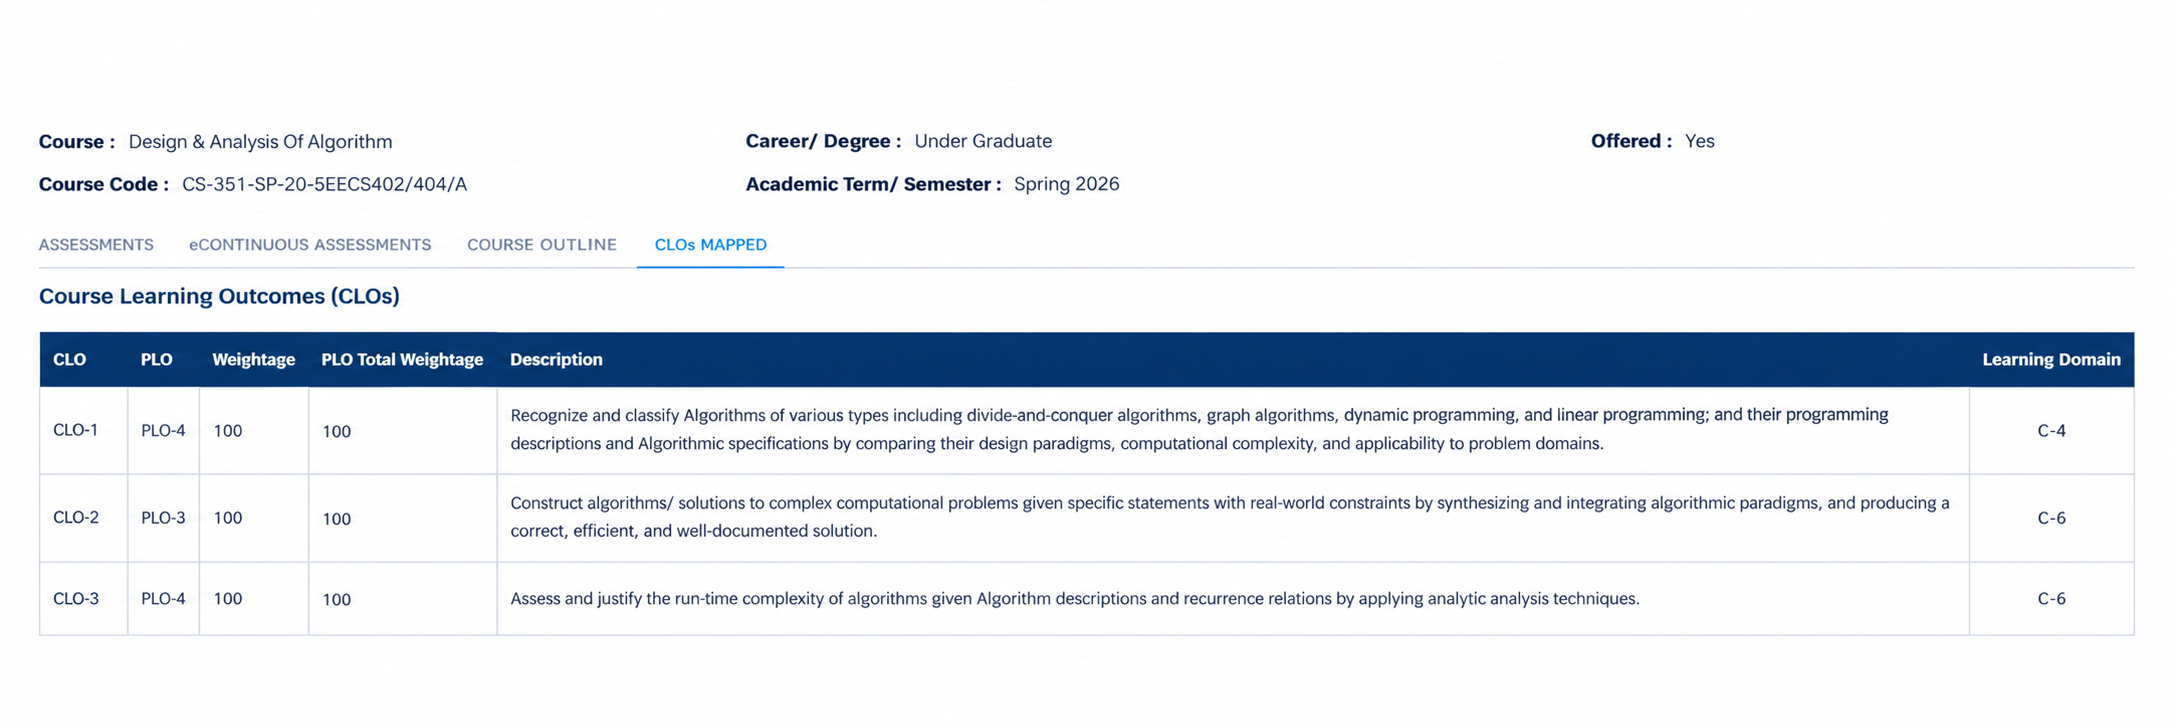
\includegraphics[width=1.0\textwidth]{images/criterion_2/media/image-7.png}
\caption{CLO-PLO Mapping of CS-251 Design and Analysis of Algorithms}
\label{figure:CLO-PLO mapping of sample course}
\end{figure}

In step 2, the total marks and weightage for each assessment are set. Then, each assessment is mapped to a pertinent CLOs with appropriate CLO weightage as shown in Figure~\ref{figure:assessments showing on qalam}. 

\begin{figure}[H]
\centering
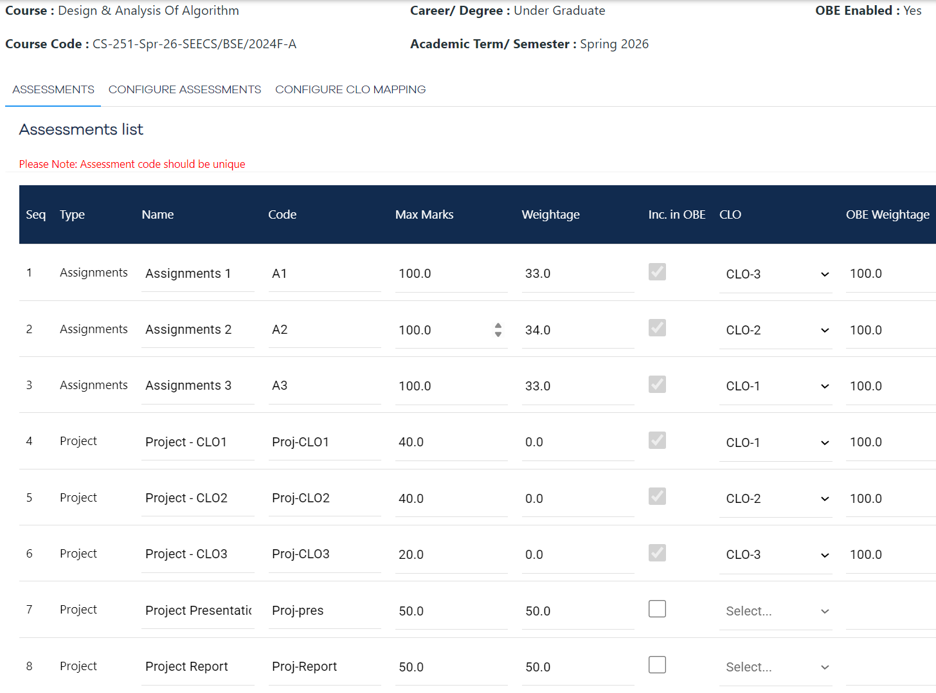
\includegraphics[width=1.0\textwidth]{images/criterion_2/media/image8.png}
\caption{Snippet of Qalam Result Section Showing Number of Assessments, their Total Marks, Weightage, and Mapping to Appropriate CLO along with the CLO Weightages}
\label{figure:assessments showing on qalam}
\end{figure}

Multiple assignments, quizes, and Mid \& End Semester Exams have been created among others. The weightage of each assessment is also set for the calculation of aggregate percentage of the course. The assessment is enabled as an OBE assessment that means the marks obtained in these assessments will be used to calculate the CLO attainment score. Appropriate CLO is mapped to each assessment, and CLO weightage is also defined (100 weightage means that each assessment has an equal weightage during CLO attainment calculations).
%\end{landscape}

After configuring the assessments, the marks obtained for each assessment are entered manually by the instructor. Once the data is entered, the result will be compiled by Qalam. The compiled result is also visible to the students. Each instructor can download the CLO and PLO attainment reports of his/her course. Annexure~\ref{Sample CLO Attainment Report} shows the CLO attainment report of CS-251 Design and Analysis of Algorithms course that highlights the CLO attainment in green and CLO not attained in red for each student. Attainment score for each CLO is also visible. The percentage CLO attainment for individuals and cohorts is then calculated. Based on the CLOs the mapped PLOs are evaluated as well in terms of `Yes' or `No' as per the defined KPIs. Annexure~\ref{Sample PLO Attainment Report} shows PLOs score and attainment for the CS-251 Design and Analysis of Algorithms course for 2024 batch.

\section{Sample CLO Attainment Report}
\label{Sample CLO Attainment Report}
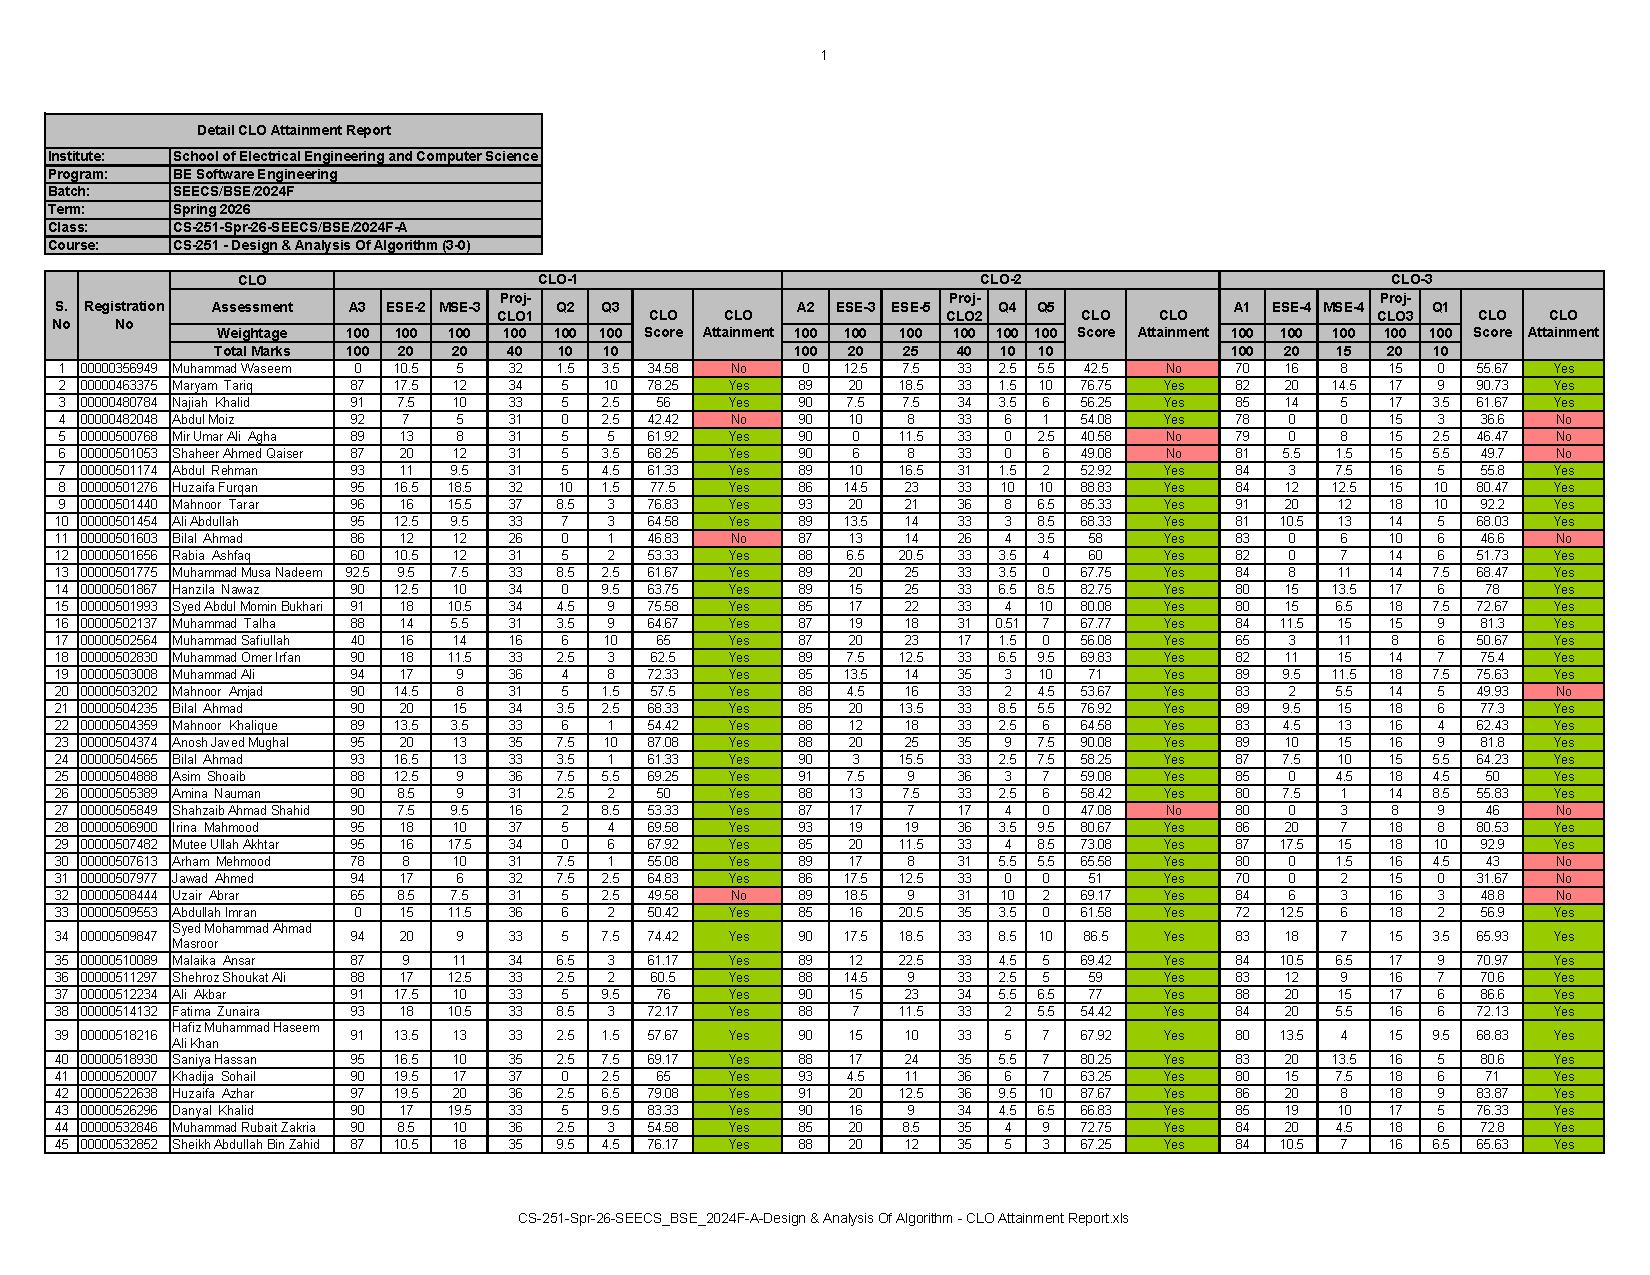
\includepdf[
    pages=-,
    landscape,
    fitpaper=true
]{appendices/criterion_2/Sample CLO Attainment Report.pdf}

\section{Sample PLO Attainment Report}
\label{Sample PLO Attainment Report}
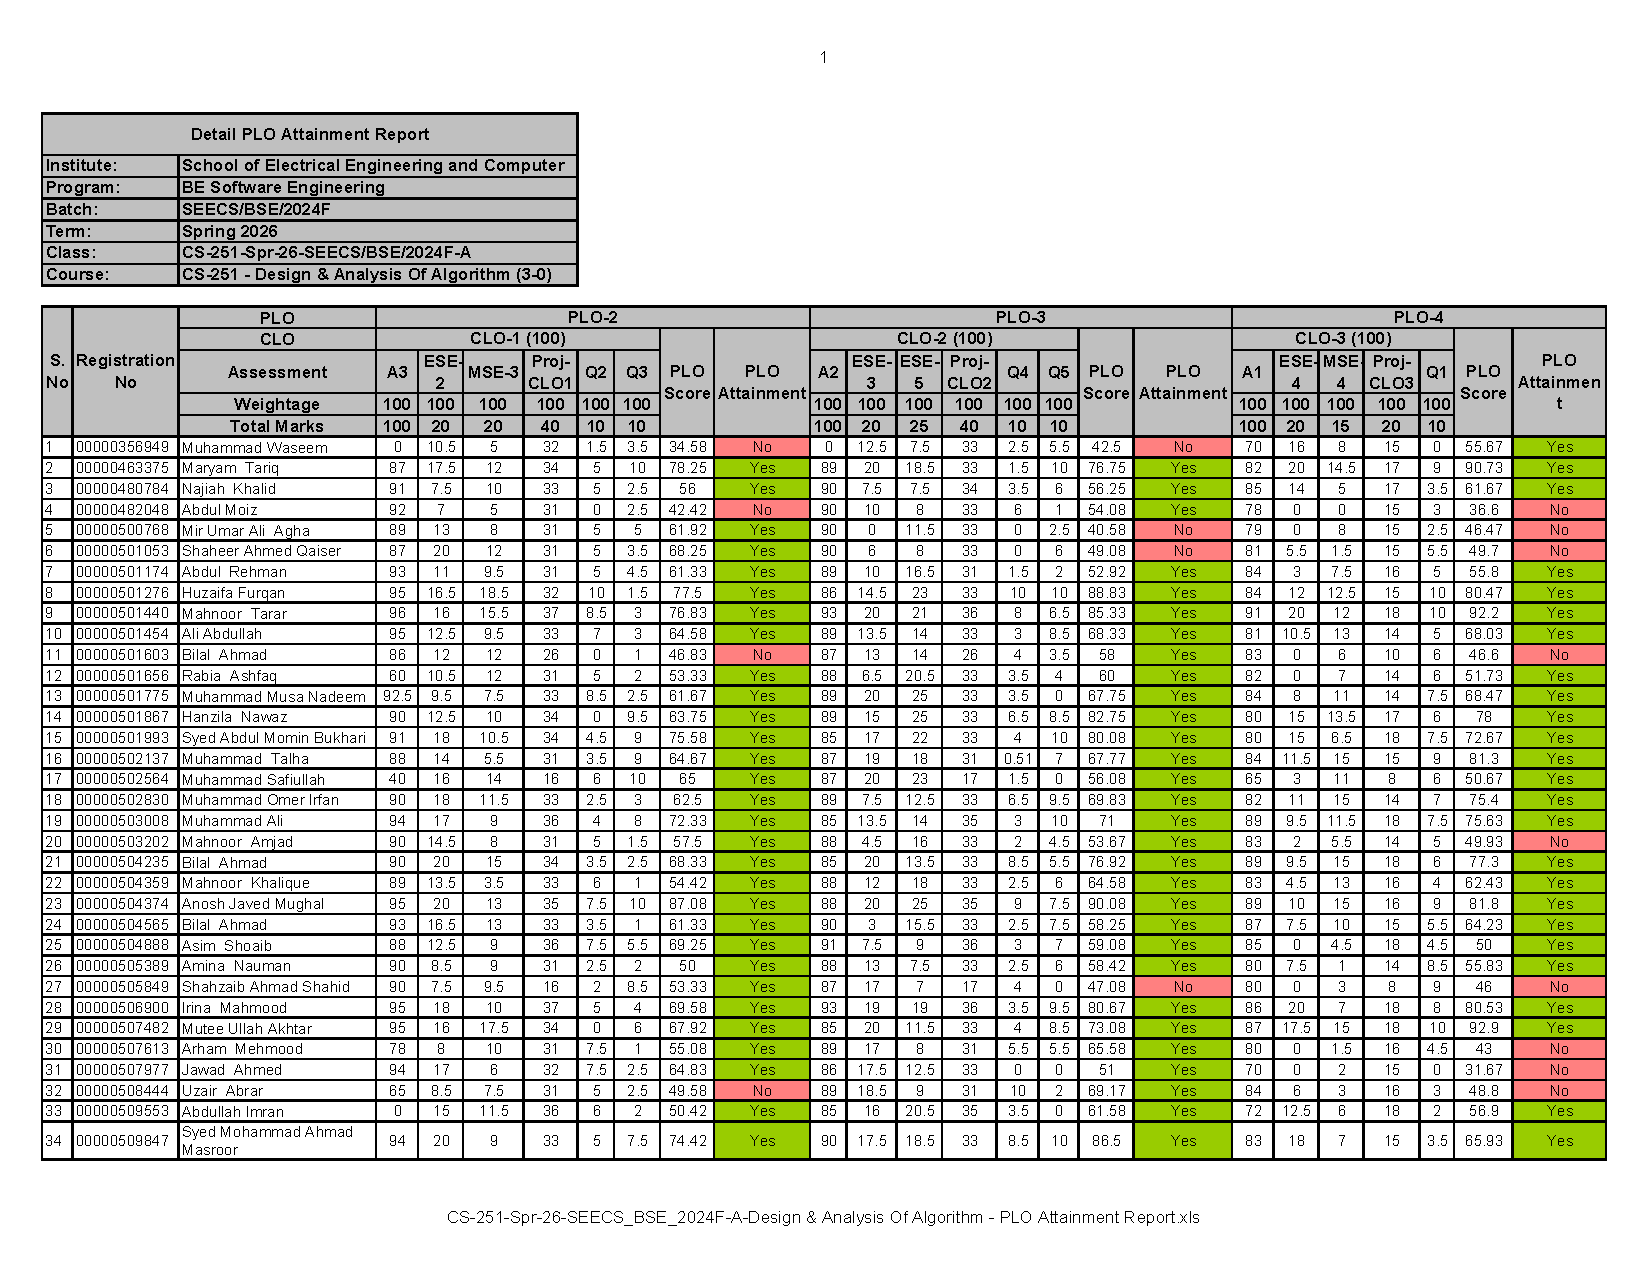
\includepdf[
   pages=-,
    landscape,
    fitpaper=true
]{appendices/criterion_2/Sample PLO Attainment Report.pdf}

\section{Consolidated PLO Attainment Report of 2K22 batch after Fall 2025 (7th Semester)}
\label{Consolidated PLO Attainment Report}
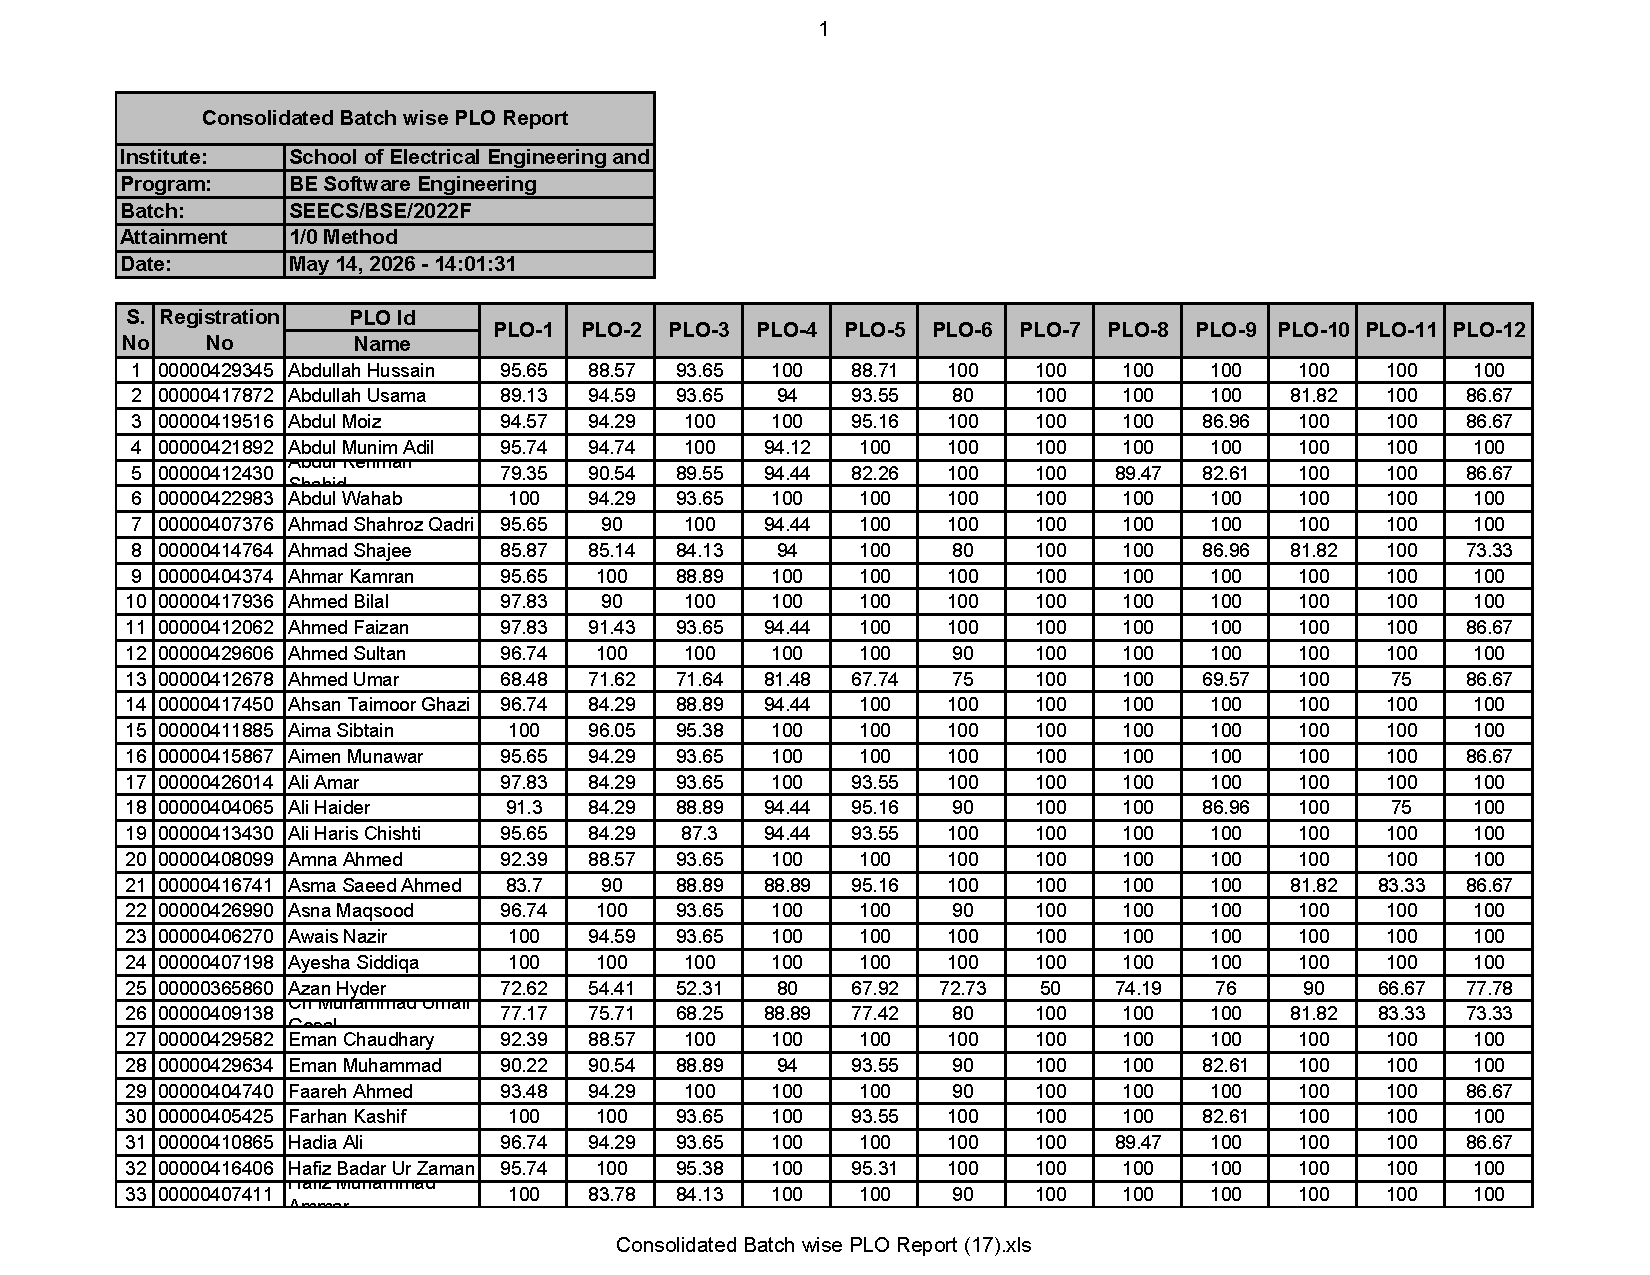
\includepdf[
    pages=-,
    landscape,
    fitpaper=true
]{appendices/criterion_2/Consolidated Batch wise PLO Report.pdf}



\clearpage
\section{CLO-PLO Attainment Results for Fall 2025 Semester}
\label{annex:clo-plo-attainment-results}
This section discusses the CLO-PLO attainment results of intake 2K22, 2K24 and 2K25 batches for Fall 2025 semester. The following subsections provides detail analysis for CLO-PLO attainment.

\subsection{2K22 Batch Fall 2025 Semester Results}

Figure~\ref{figure:2K22-batch-clo-plo-results} shows a screenshot of spreadsheet for all the courses taken by 2K22 batch in Fall 2025 semester. The figure contains CLO-PLO mapping and percentage of CLO attainment that is directly imported from the individual CLO and PLO attainment reports of each course from Qalam. Figure~\ref{figure:2022 Batch cohort CLO attainment} shows same information as bar chart showing percentage attainment of corresponding CLOs against each course. Figure~\ref{figure:2022 Batch cohort CLO attainment} also shows calculation of PLOs attainment as ``Ys'' as well as in percentage. The same information is given for PLO percentages and overall batch PLO attainment percentage in Figure~\ref{figure:2022 Batch course-wise PLO attainment} and Figure~\ref{figure:2022 Batch cohort PLO attainment}, respectively. It can be seen that the cohort has successfully attained the concerned CLOs for each course. Similarly, the cohort PLOs have been attained as per set KPIs.

\begin{figure}[H]
\centering
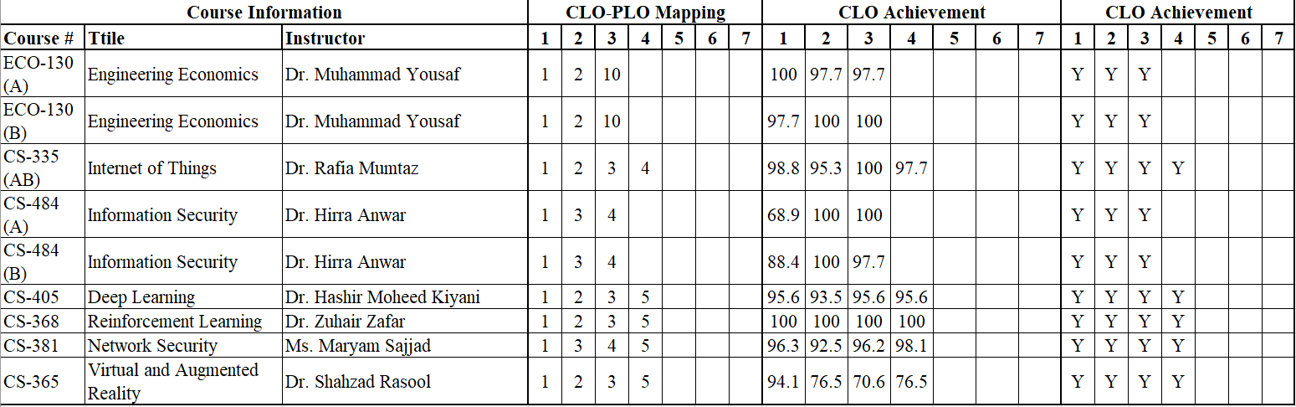
\includegraphics[width=0.98\linewidth]{images/criterion_2/media/image13.png}
\par\medskip
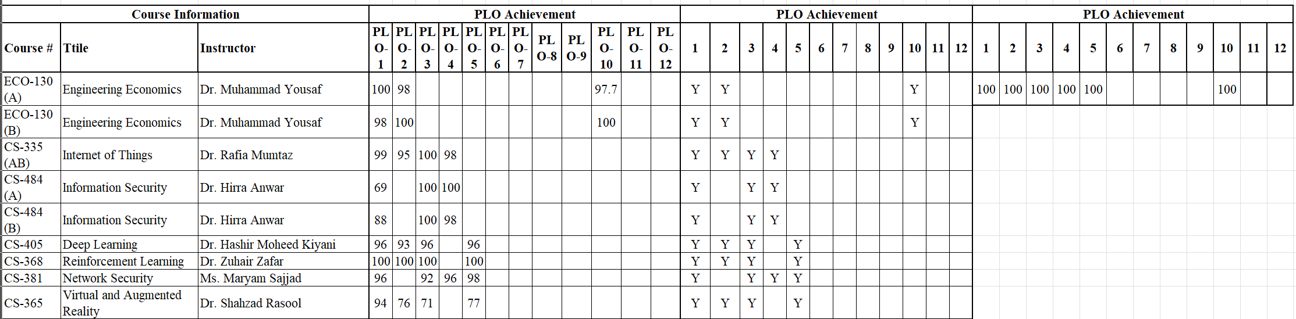
\includegraphics[width=0.98\linewidth]{images/criterion_2/media/image14.png}
\caption{ 2K22 Batch Result for All Courses in Fall 2025 Semester}
\label{figure:2K22-batch-clo-plo-results}
\end{figure}

\begin{figure}[H]
\centering
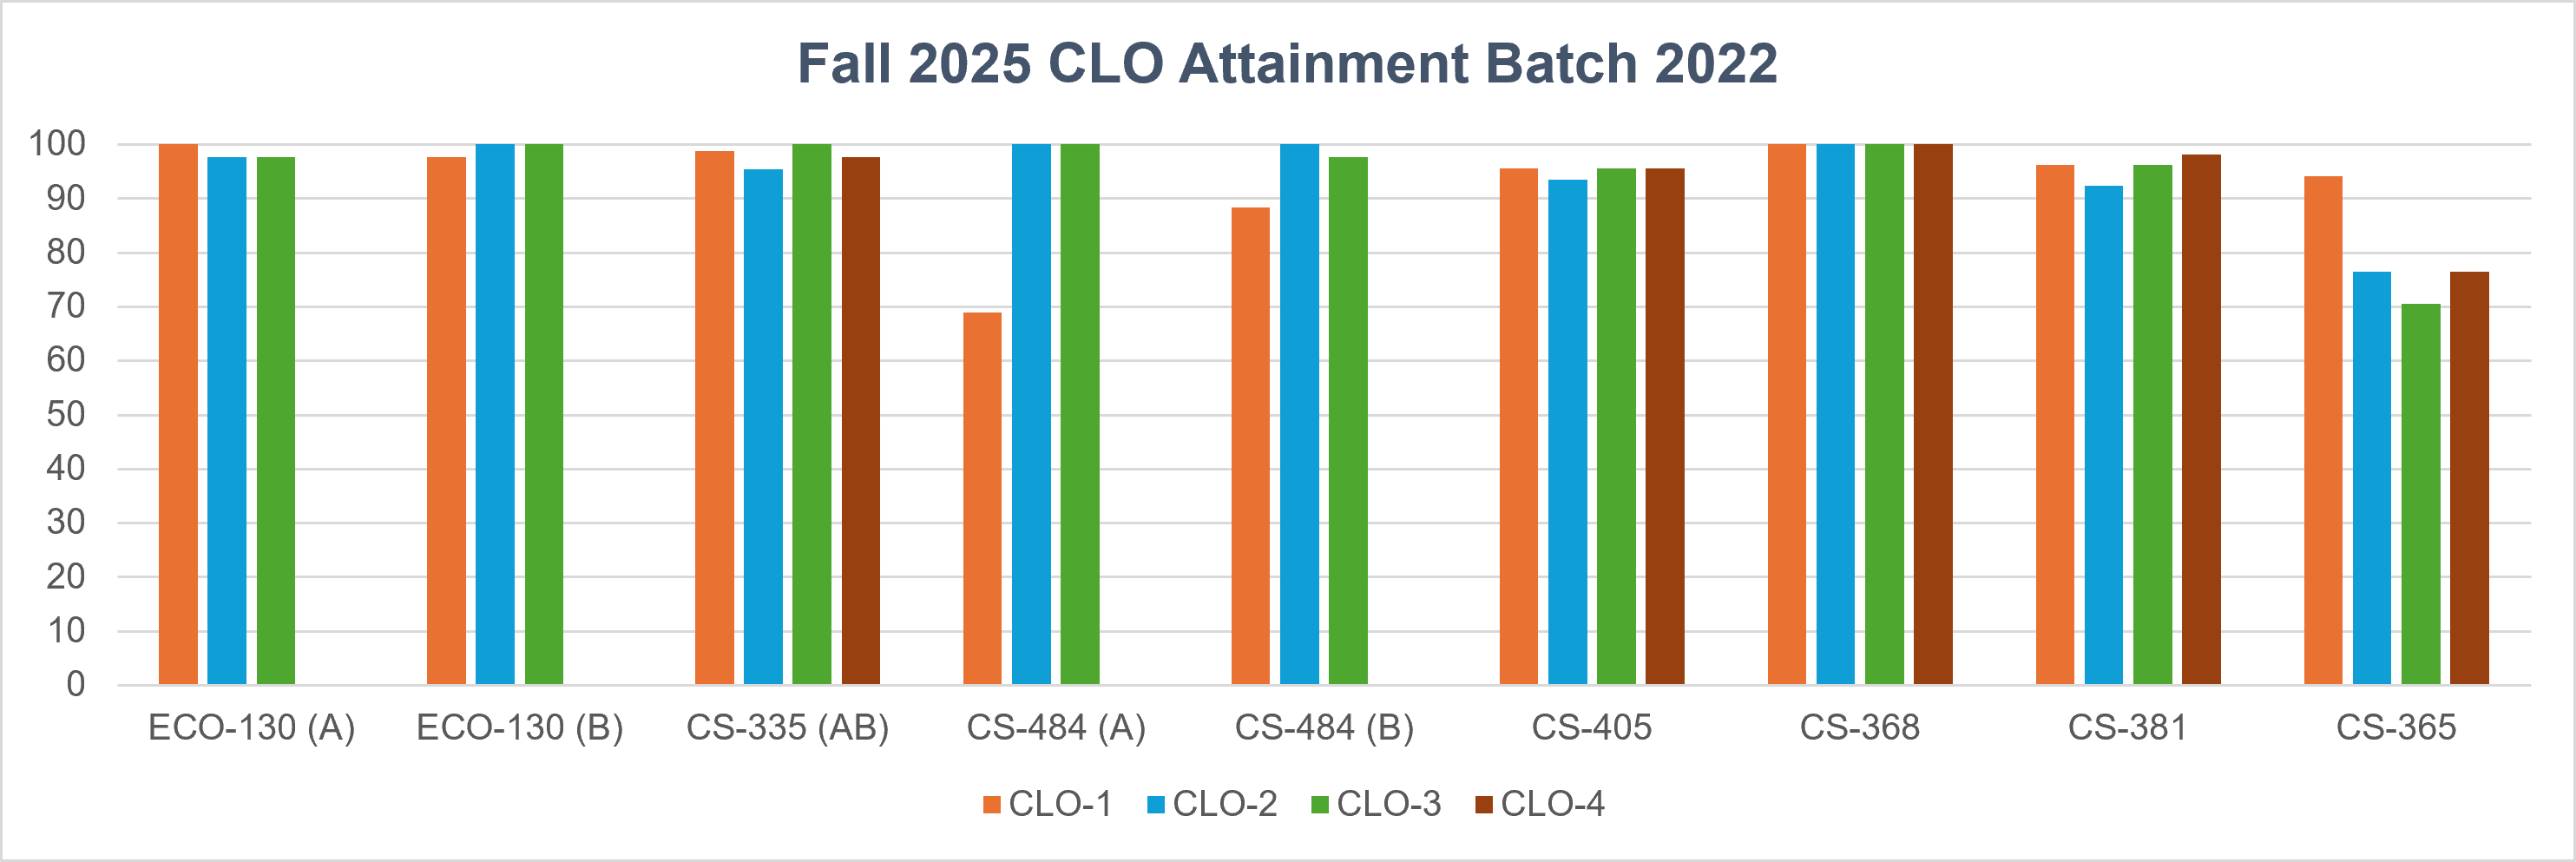
\includegraphics[width=0.95\textwidth]{images/criterion_2/media/image23.png}
\caption{2K22 Batch cohort CLO attainment for all courses in Fall 2025.}
\label{figure:2022 Batch cohort CLO attainment}
\end{figure}

\begin{figure}[H]
\centering
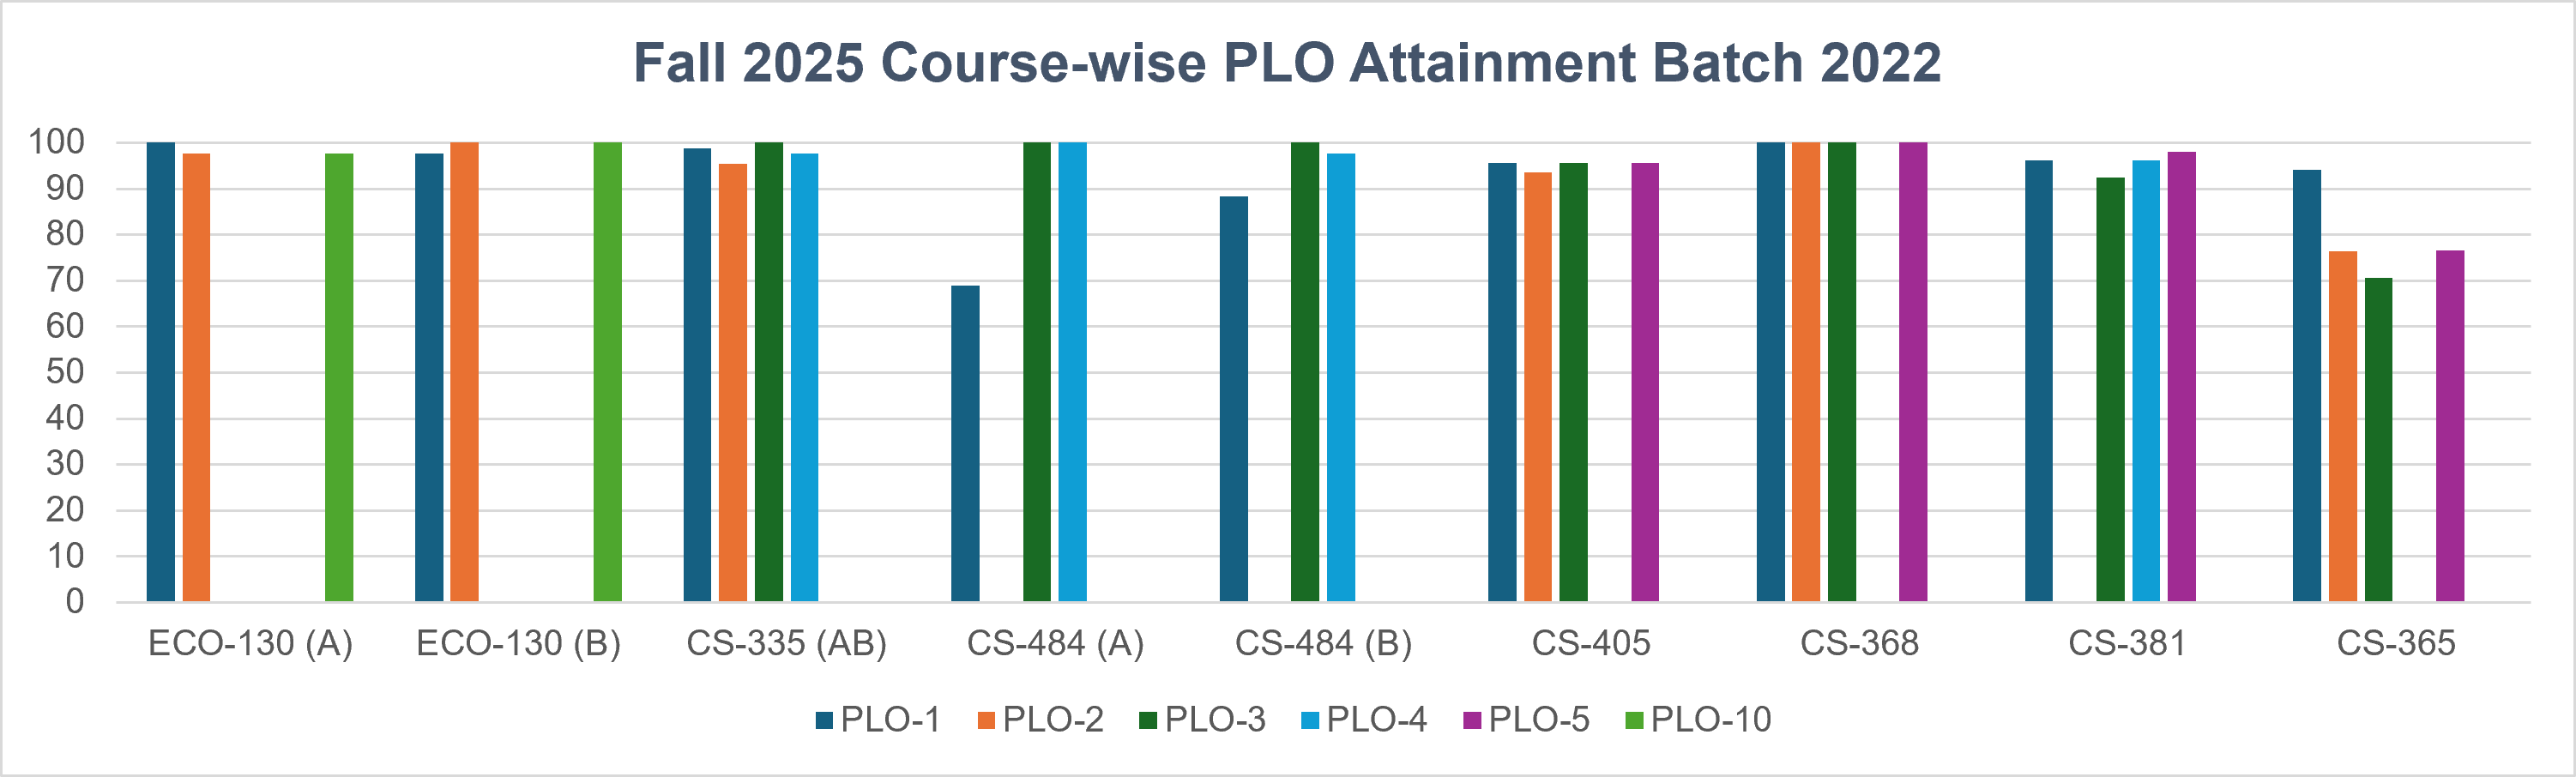
\includegraphics[width=0.95\textwidth]{images/criterion_2/media/image24.png}
\caption{2K22 Batch course-wise PLO attainment for Fall 2025.}
\label{figure:2022 Batch course-wise PLO attainment}
\end{figure}

\begin{figure}[H]
\centering
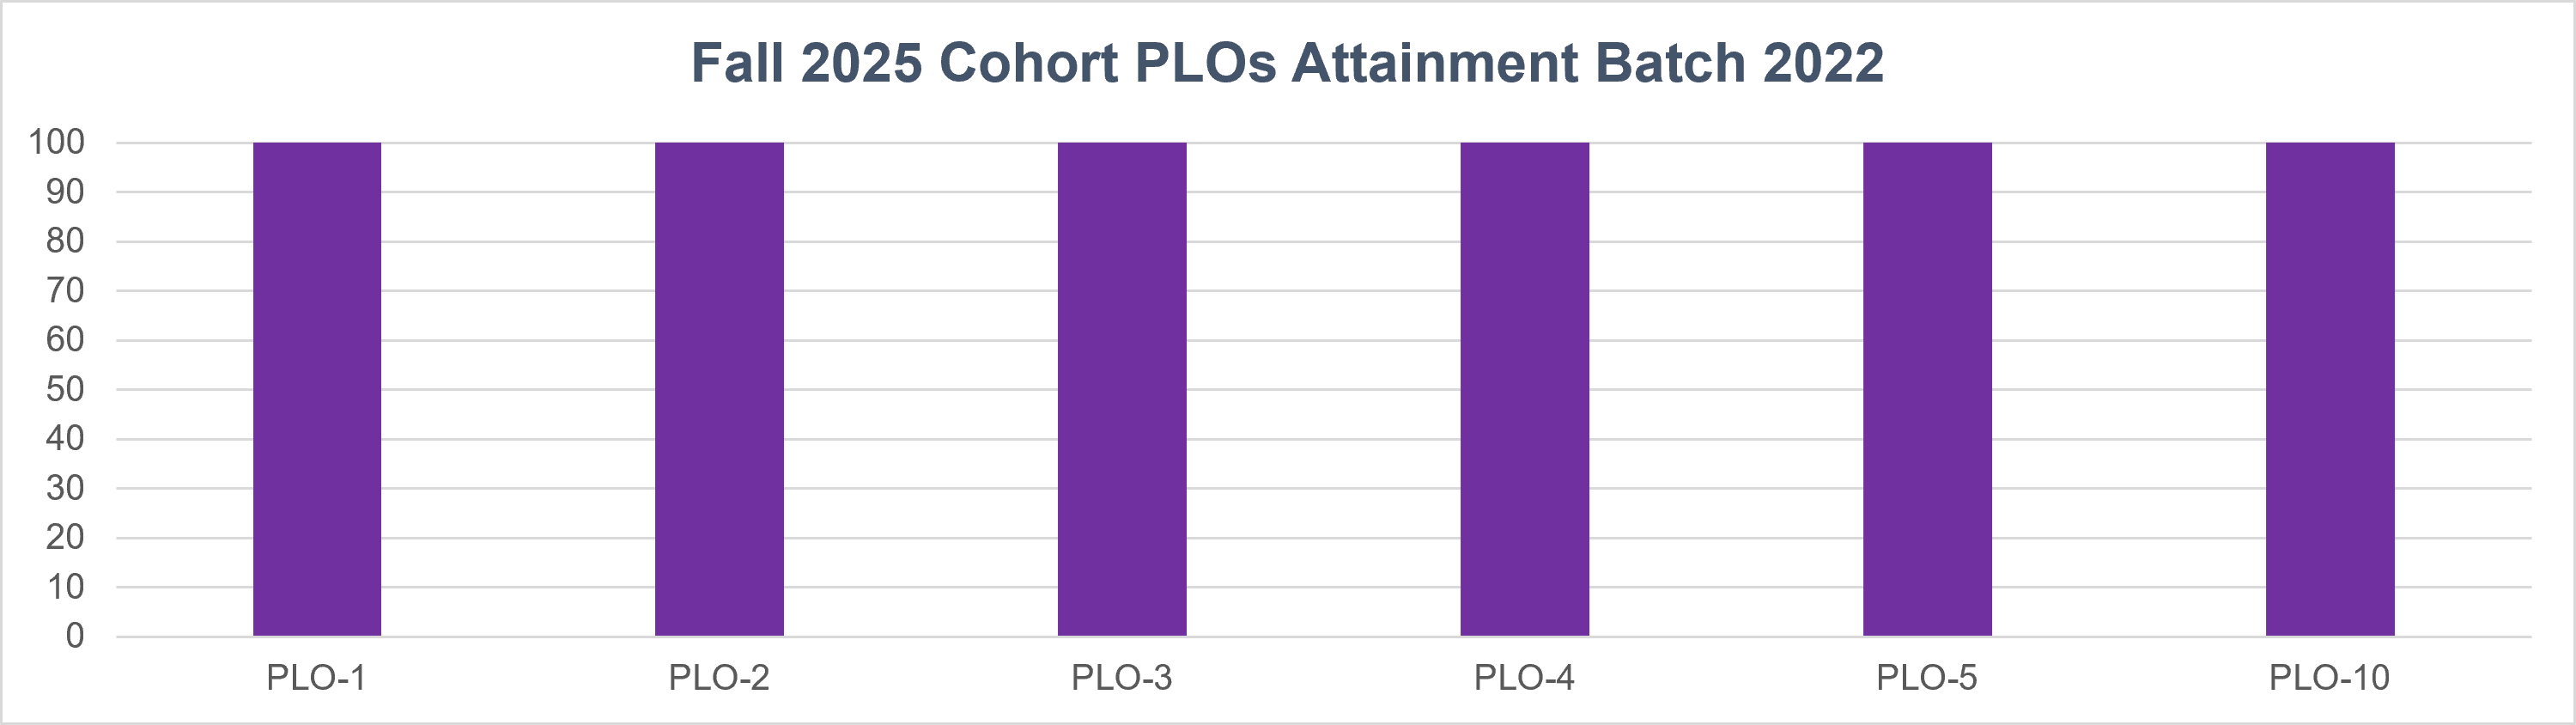
\includegraphics[width=0.95\textwidth]{images/criterion_2/media/image25.png}
\caption{2K22 Batch cohort PLO attainment against the 60\% KPI.}
\label{figure:2022 Batch cohort PLO attainment}
\end{figure}

\subsection{2K24 Batch Fall 2025 Semester Results}

The results for 2K24 batch are given in Figure~\ref{figure:2024 Batch Result for All Courses} to Figure~\ref{figure:2024 Batch cohort PLO attainment against}. It can be seen that the 2K24 batch has attained the assessed CLOs as well as the mapped PLOs on cohort level as per the set KPIs.

\begin{figure}[H]
\centering
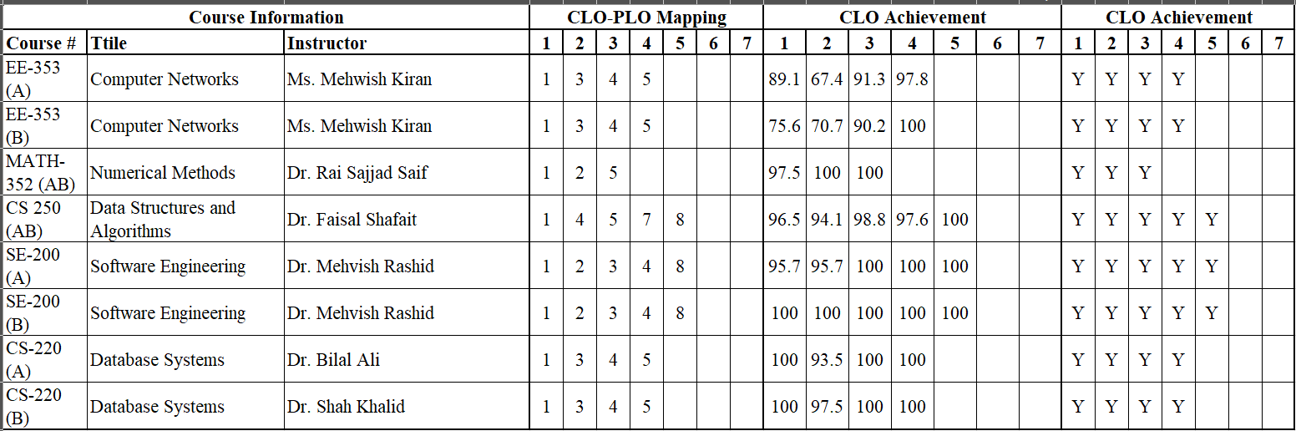
\includegraphics[width=0.98\linewidth]{images/criterion_2/media/image26.png}
\par\medskip
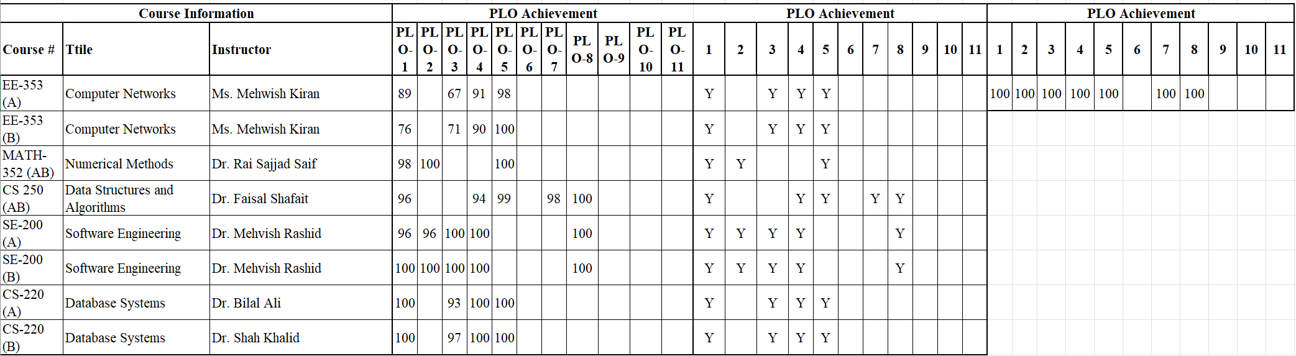
\includegraphics[width=0.98\linewidth]{images/criterion_2/media/image27.png}
\caption{2K24 Batch Result for All Courses in Fall 2025 Semester}
\label{figure:2024 Batch Result for All Courses}
\end{figure}

\begin{figure}[H]
\centering
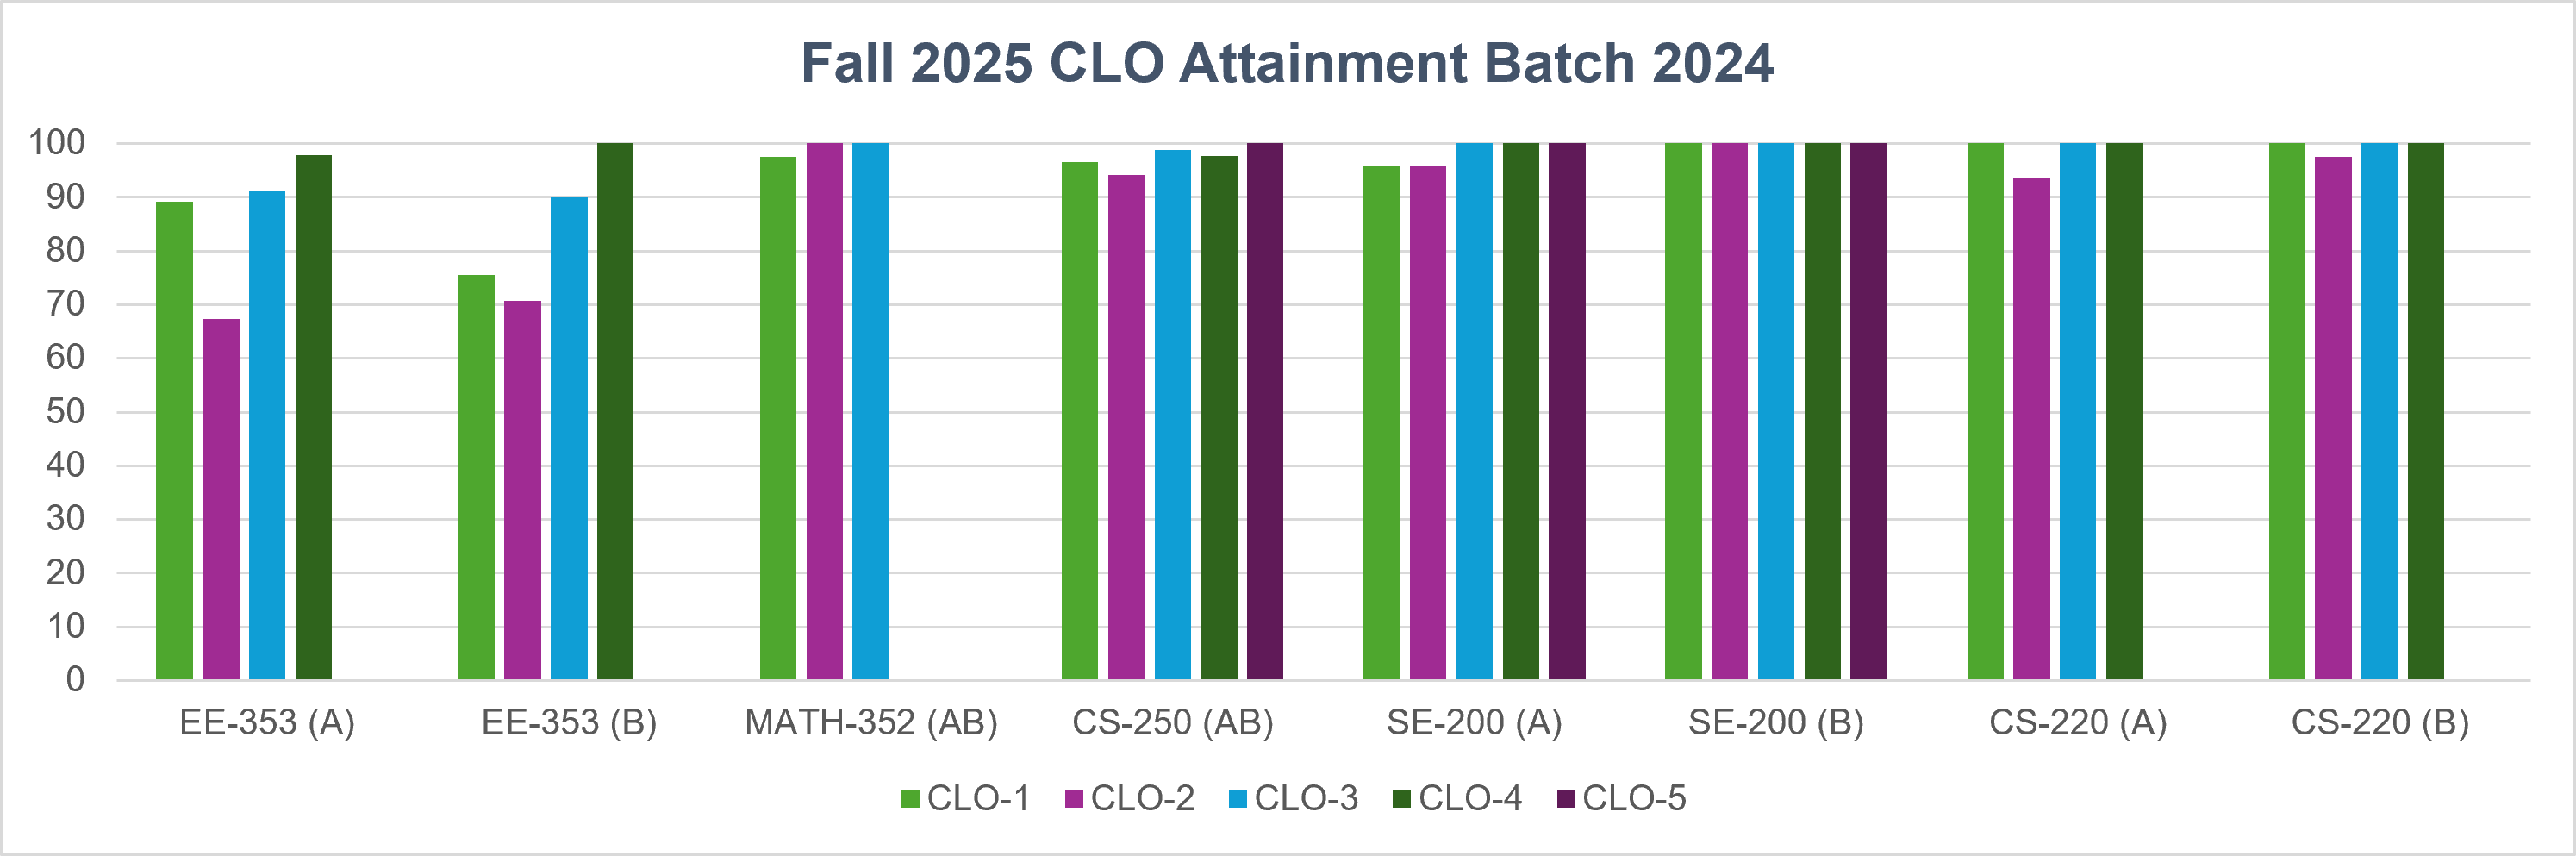
\includegraphics[width=0.95\textwidth]{images/criterion_2/media/image28.png}
\caption{2K24 Batch cohort CLO attainment for all courses in Fall 2025.}
\end{figure}

\begin{figure}[H]
\centering
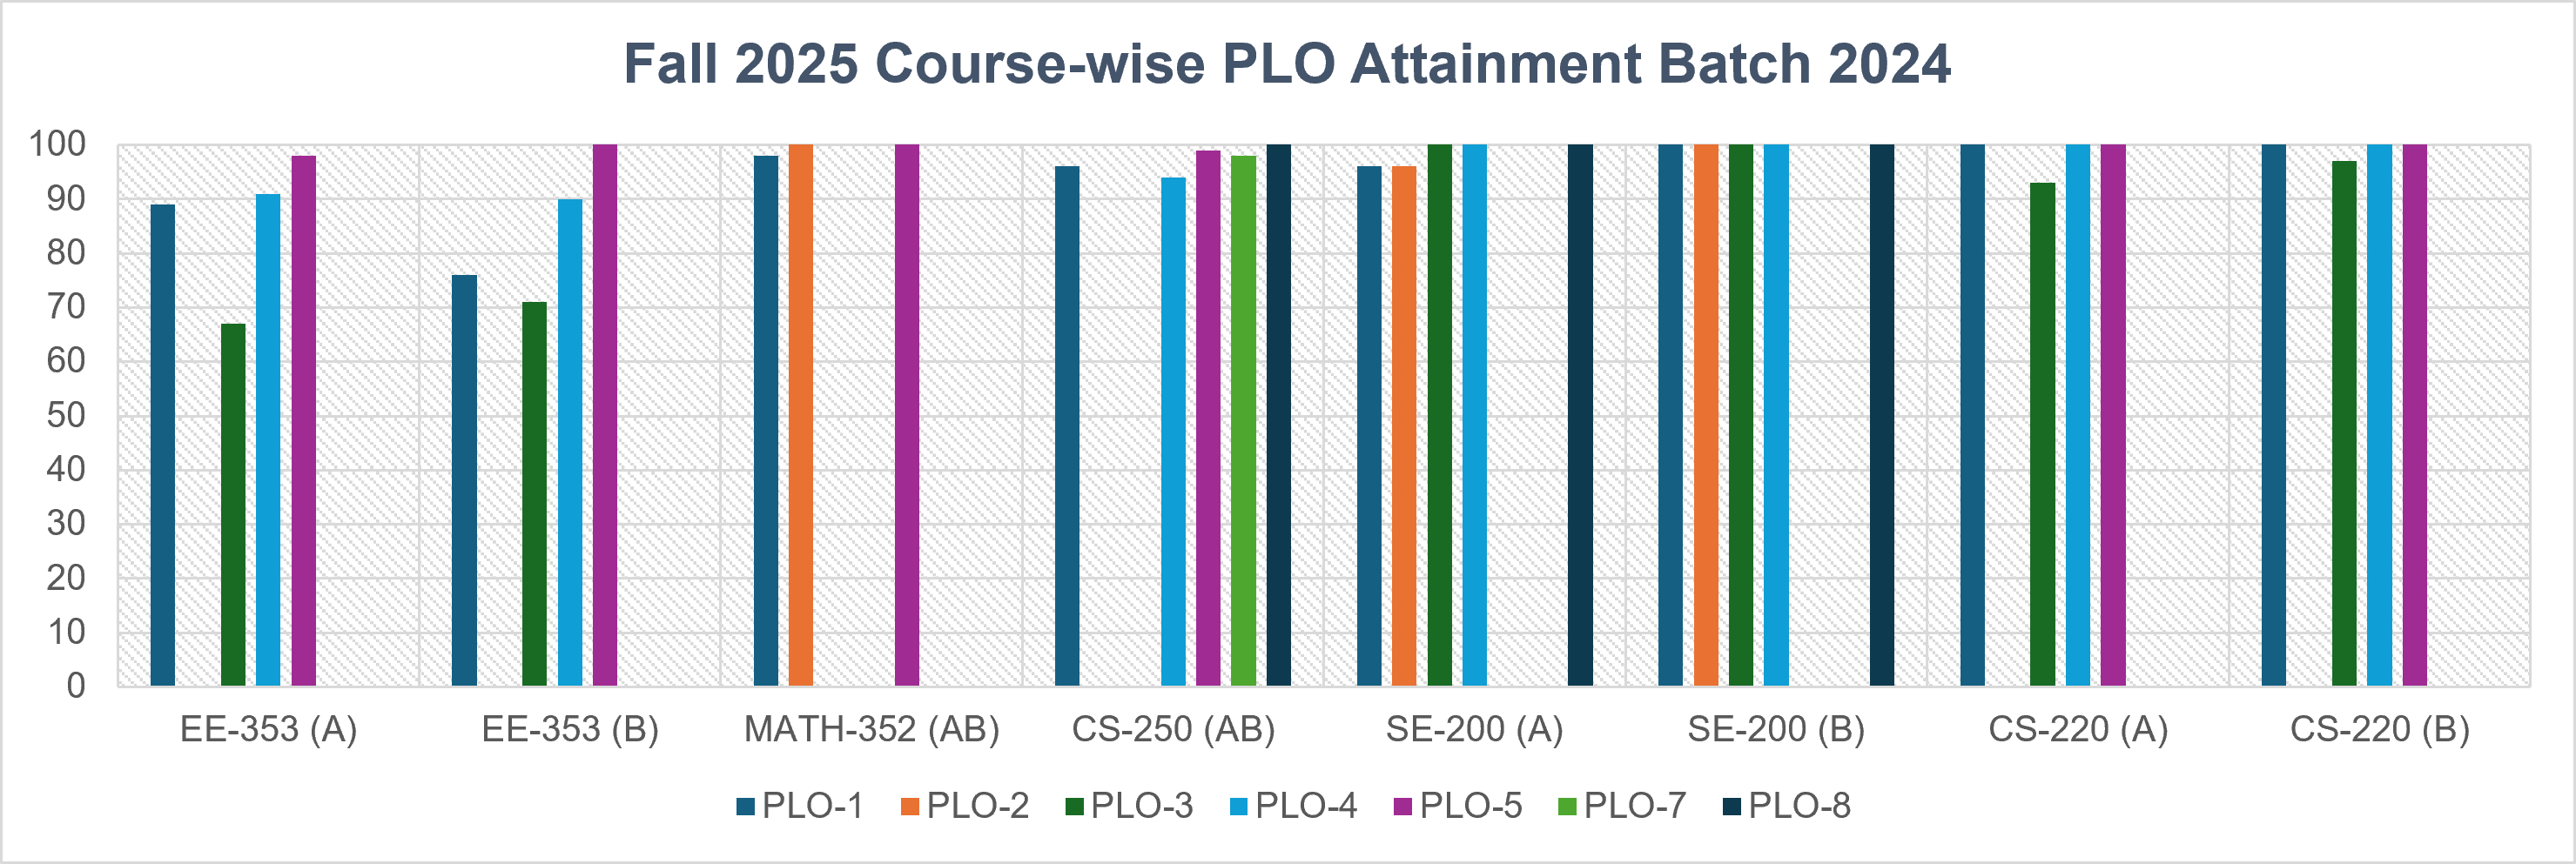
\includegraphics[width=0.95\textwidth]{images/criterion_2/media/image29.png}
\caption{2K24 Batch course-wise PLO attainment for Fall 2025}
\end{figure}

\begin{figure}[H]
\centering
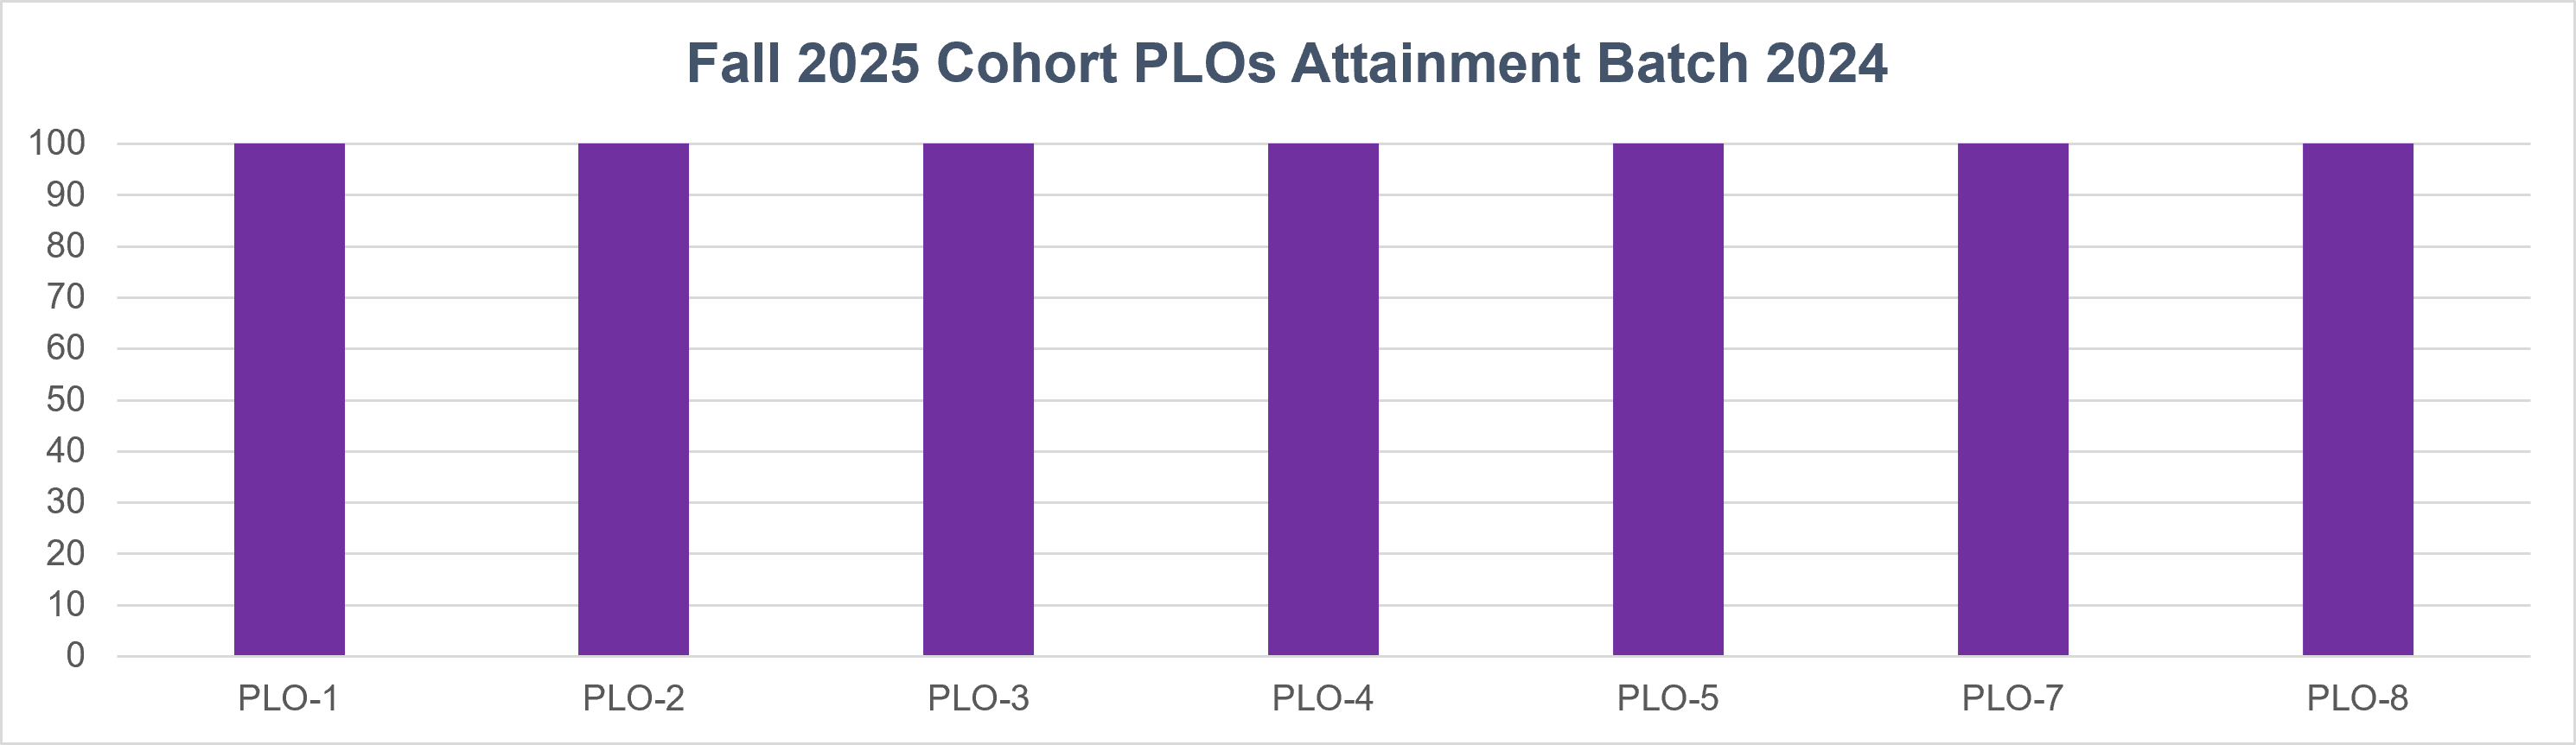
\includegraphics[width=0.95\textwidth]{images/criterion_2/media/image30.png}
\caption{2K24 Batch cohort PLO attainment against the 60\% KPI.}
\label{figure:2024 Batch cohort PLO attainment against}
\end{figure}

\subsection{2K25 Batch Fall 2025 Semester Results}

The results for 2K25 batch are given in Figure~\ref{figure:2025 Batch Result for All Courses} to Figure~\ref{figure:2025 Batch cohort PLO attainment}. It can be seen that the 2K25 batch has attained the assessed CLOs as well as the mapped PLOs on cohort level as per the set KPIs.

\begin{figure}[H]
\centering
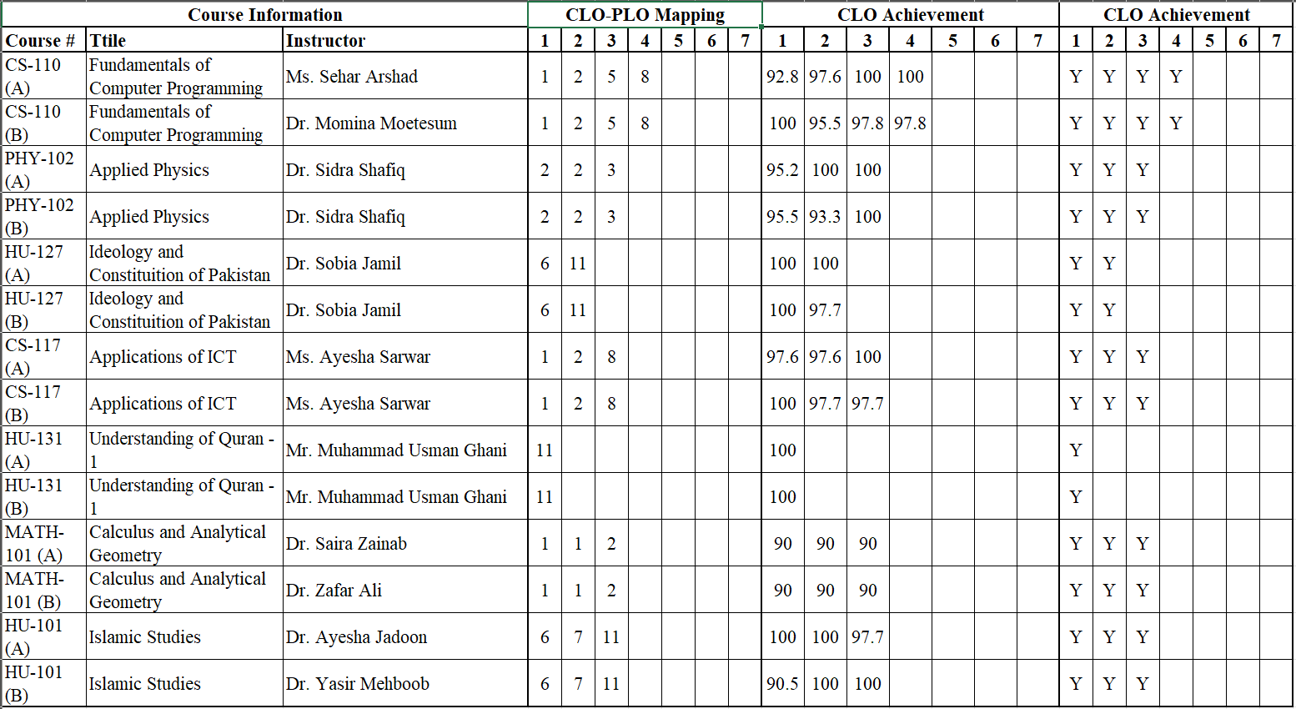
\includegraphics[width=0.98\linewidth]{images/criterion_2/media/image31.png}
\par\medskip
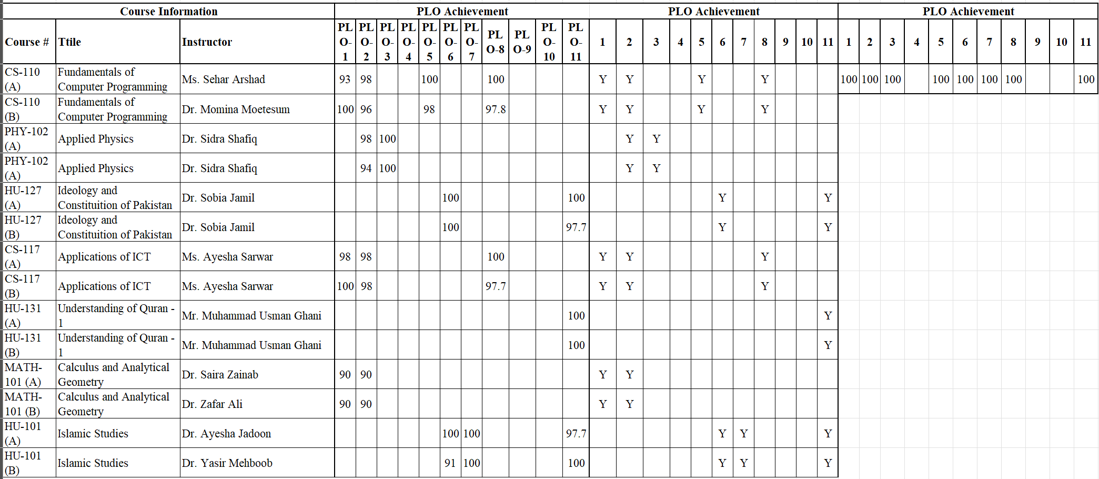
\includegraphics[width=0.98\linewidth]{images/criterion_2/media/image32.png}
\caption{2K25 Batch Result for All Courses in Fall 2025 Semester}
\label{figure:2025 Batch Result for All Courses}
\end{figure}

\begin{figure}[H]
\centering
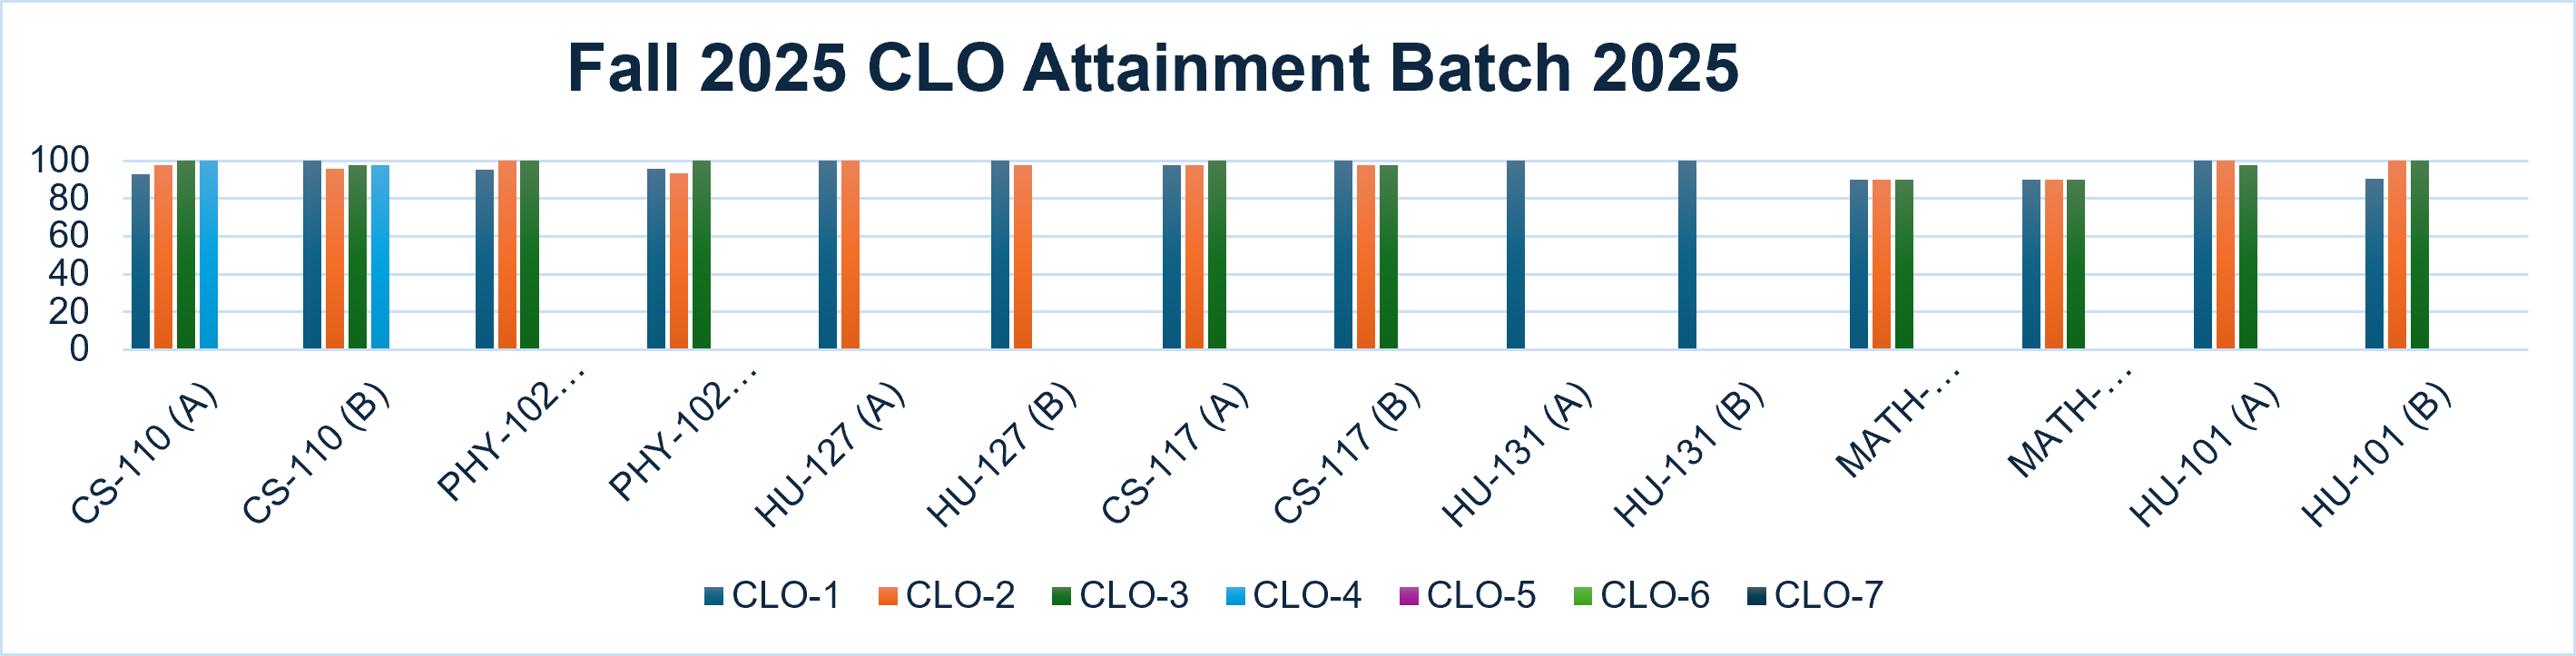
\includegraphics[width=0.95\textwidth]{images/criterion_2/media/image33.png}
\caption{2K25 Batch cohort CLO attainment for all courses in Fall 2025.}
\end{figure}

\begin{figure}[H]
\centering
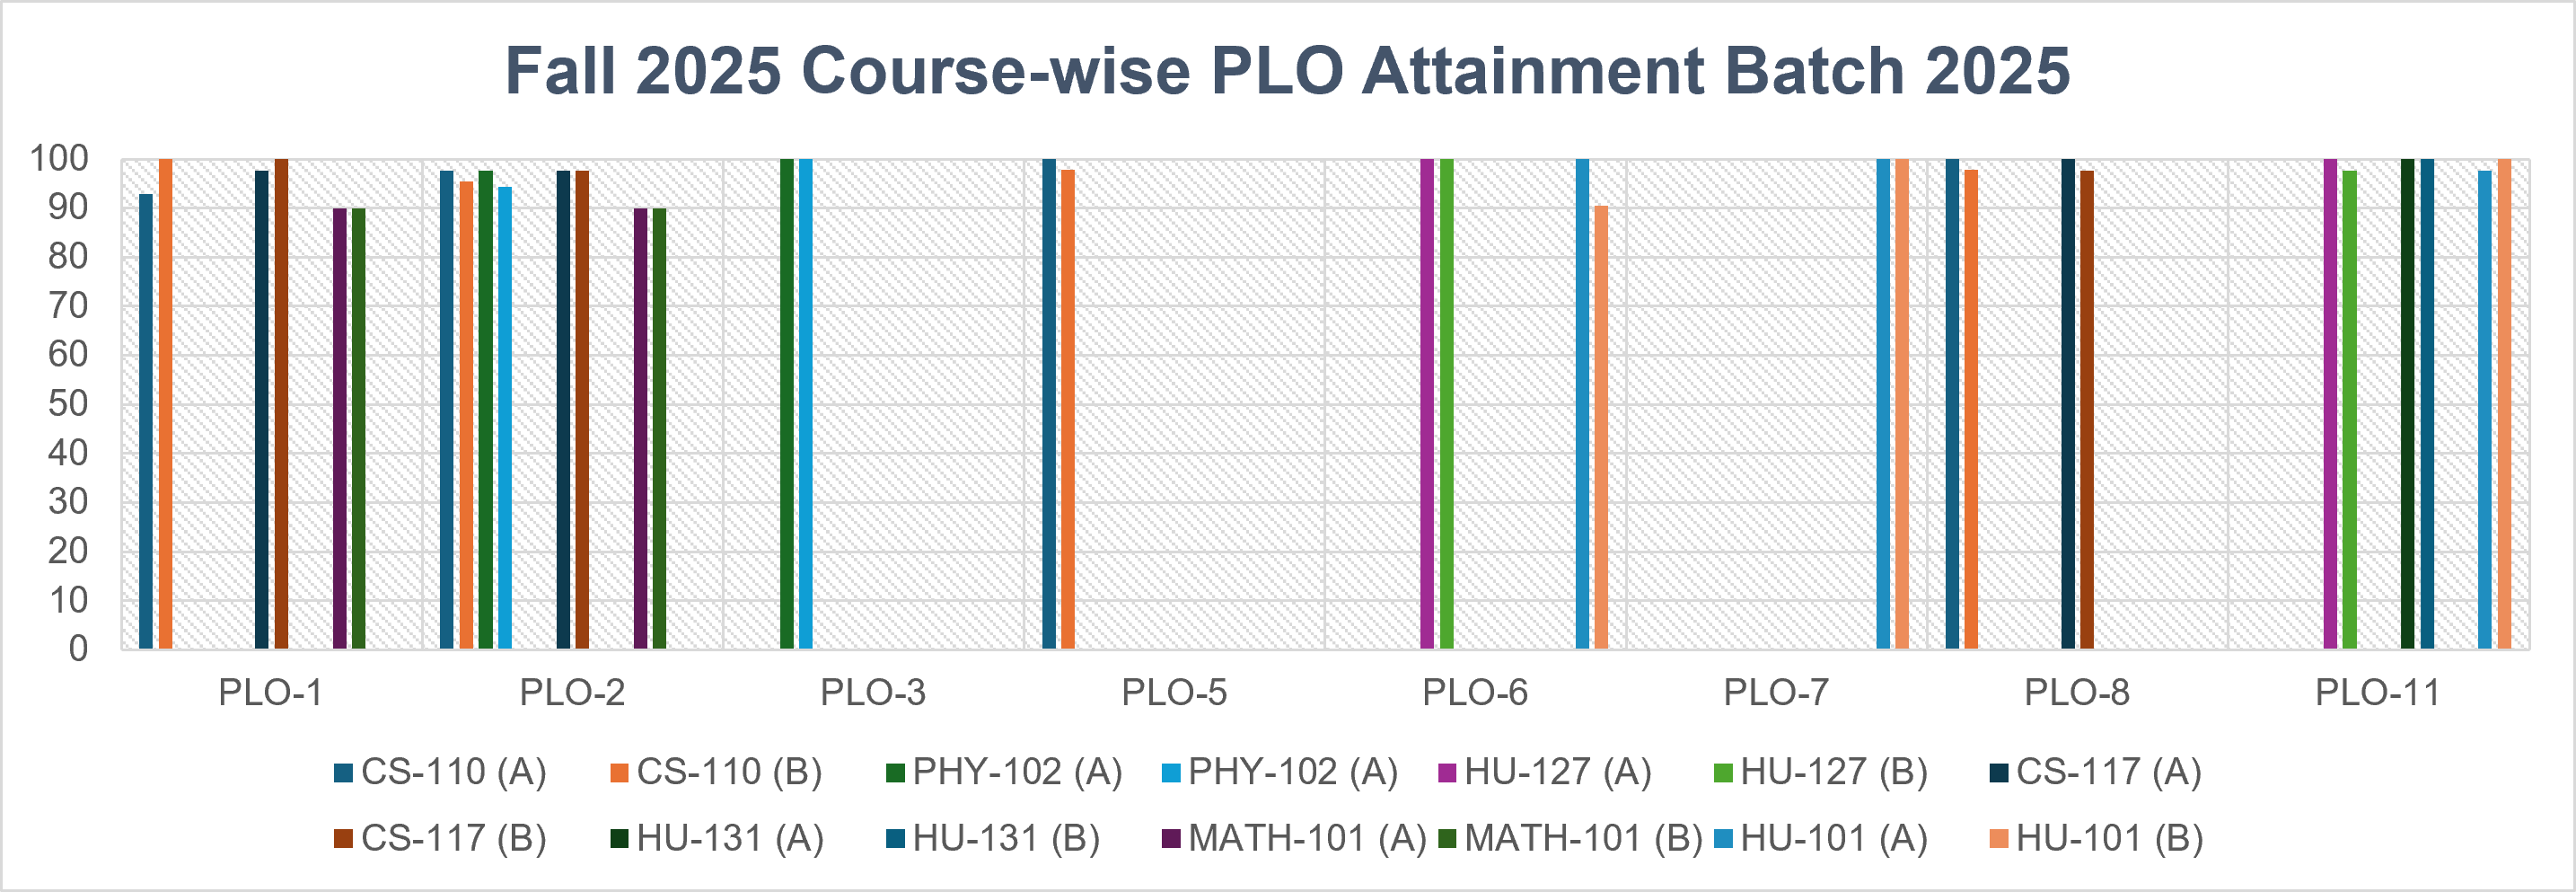
\includegraphics[width=0.95\textwidth]{images/criterion_2/media/image34.png}
\caption{2K25 Batch course-wise PLO attainment for Fall 2025.}
\end{figure}

\begin{figure}[H]
\centering
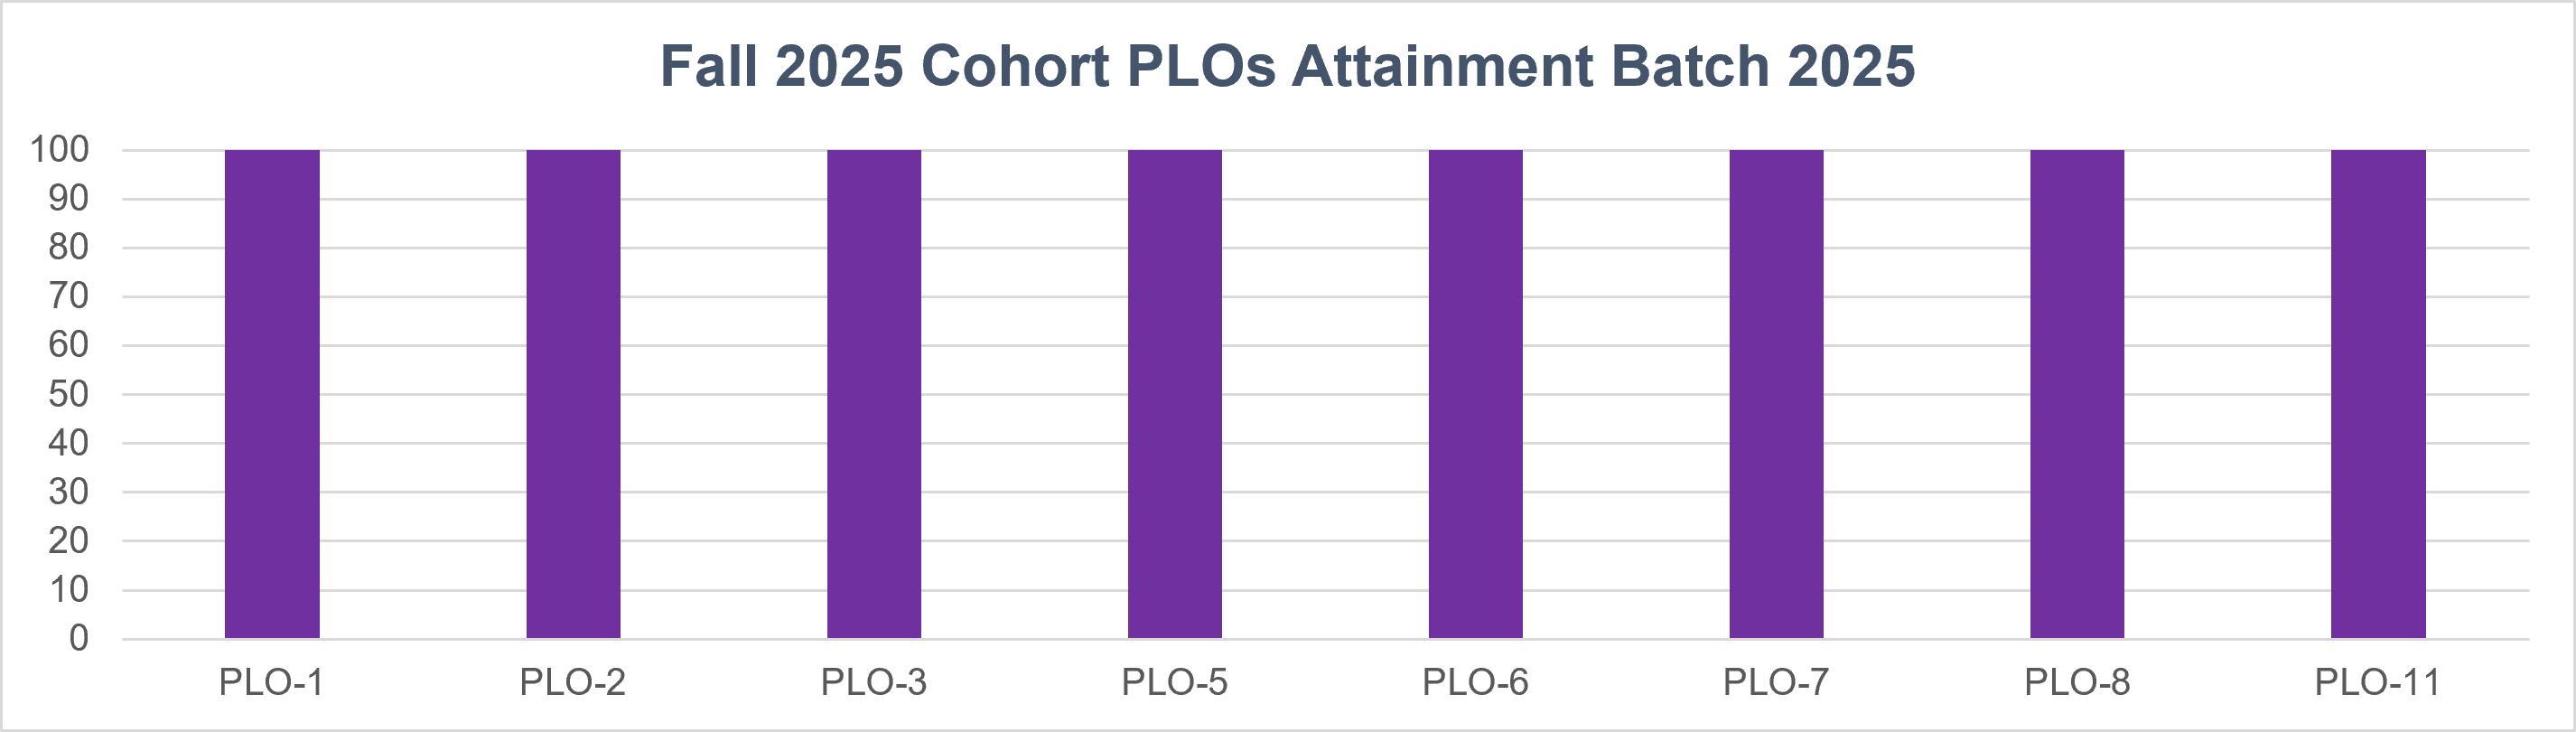
\includegraphics[width=0.95\textwidth]{images/criterion_2/media/image35.png}
\caption{2K25 Batch cohort PLO attainment against the 60\% KPI.}
\label{figure:2025 Batch cohort PLO attainment}
\end{figure}

\section{Internship Feedback Form}
\label{annex:internship-feedback-form}
%\includefullannexure{appendices/criterion_2/Internship Feedback Form.pdf}
\begin{figure}[H]
\centering
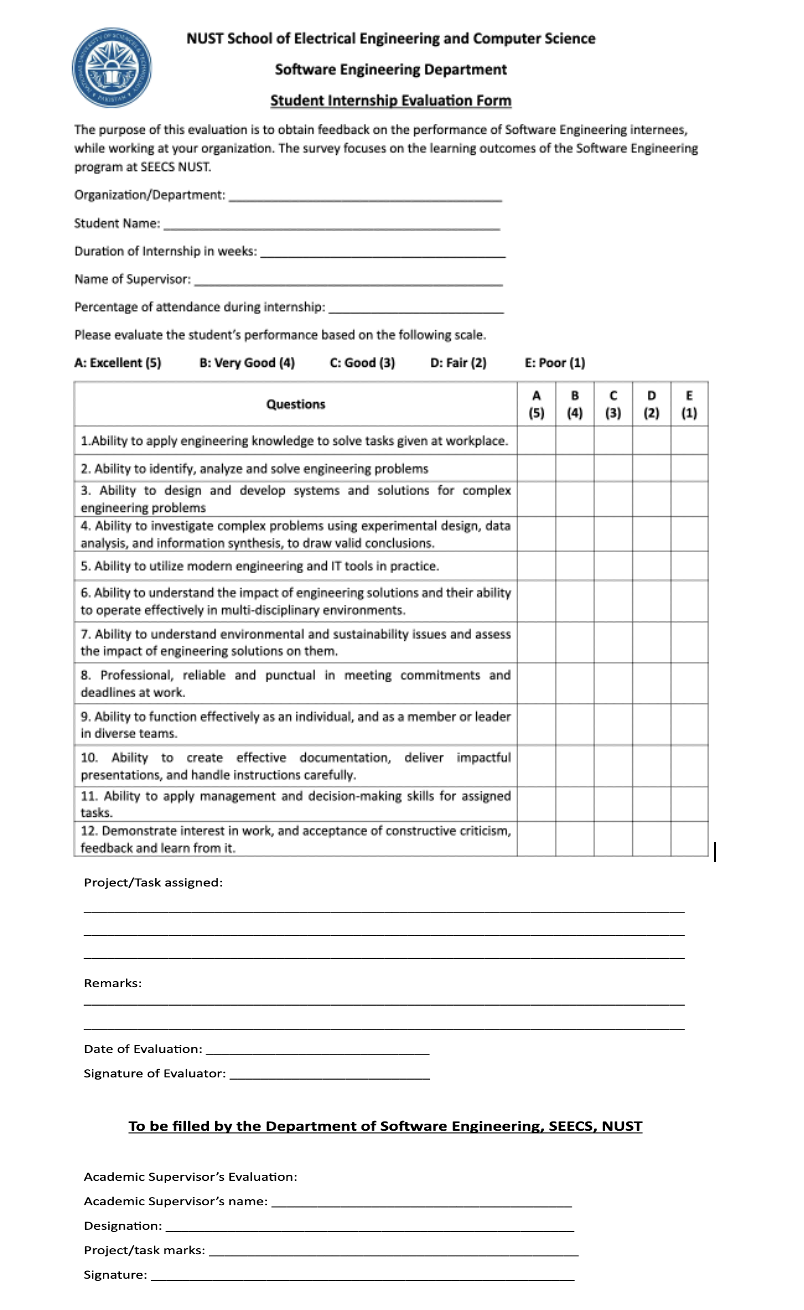
\includegraphics[width=1.0\textwidth]{images/criterion_2/media/internship form.png}
\caption{Internship Feedback Form}
\label{figure:internship form}
\end{figure}

\section{Internship Feedback Analysis}
\label{annex:internship-feedback-analysis}
This analysis evaluates the attainment of Program Learning Outcomes (PLOs) for the Bachelor of Engineering in Software Engineering (BESE) program across three consecutive intake batches: 2K21, 2K22, and 2K23. The assessment is based on industry employer feedback collected via a 5-point Likert scale (where 5 is the highest/excellent and 1 is the lowest/poor) during student internships. The sample sizes for the feedback is given in Figure~\ref{fig:internship-sample-sizes}.

\begin{figure}[H]
\centering
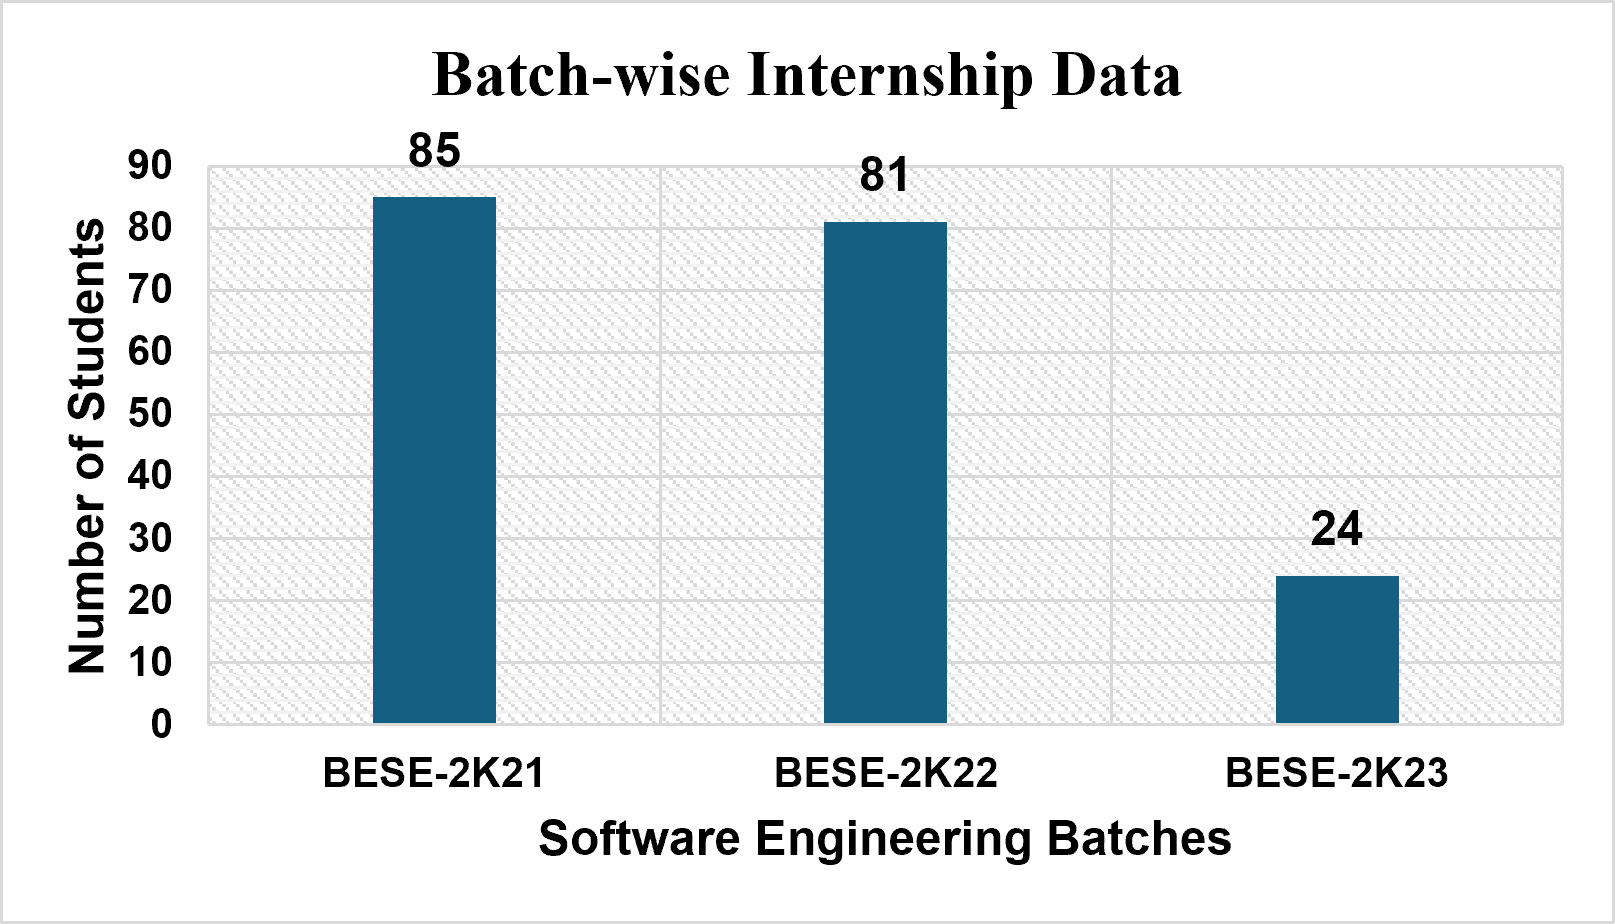
\includegraphics[width=0.78\textwidth]{images/criterion_2/media/image36.png}
\caption{Batch-wise sample sizes for internship employer feedback.}
\label{fig:internship-sample-sizes}
\end{figure}

\subsection{Batch-Wise PLO Attainment Performance}

\textbf{1.\ Batch 2K21 Analysis}

Employers overall rated the 2K21 batch very highly, with negligible negative feedback (scores of 1 or 2) across almost all outcomes. Figure~\ref{figure:PLO attainment based on internship 2K21} shows the average PLO attainment plots for the BESE 2K21 batch. Table~\ref{table:PLO attainment based on internship 2K21} shows the number of employer responses obtained for each rubric.

\begin{itemize}
\item \textbf{Highest Attainment:} \textbf{PLO 11} (Management and decision-making; 46 scores of 5) and \textbf{PLO 12} (Interest in work and handling feedback; 43 scores of 5). This indicates strong soft skills, adaptability, and professional maturity.
\item \textbf{Areas for Growth:} \textbf{PLO 3} (Design and development; 29 scores of 5) and \textbf{PLO 4} (Investigation of complex problems; 30 scores of 5) received slightly lower top-tier scores, showing that while students are competent, complex problem-solving and deep engineering design require further reinforcement.
\end{itemize}

\begin{figure}[H]
\centering
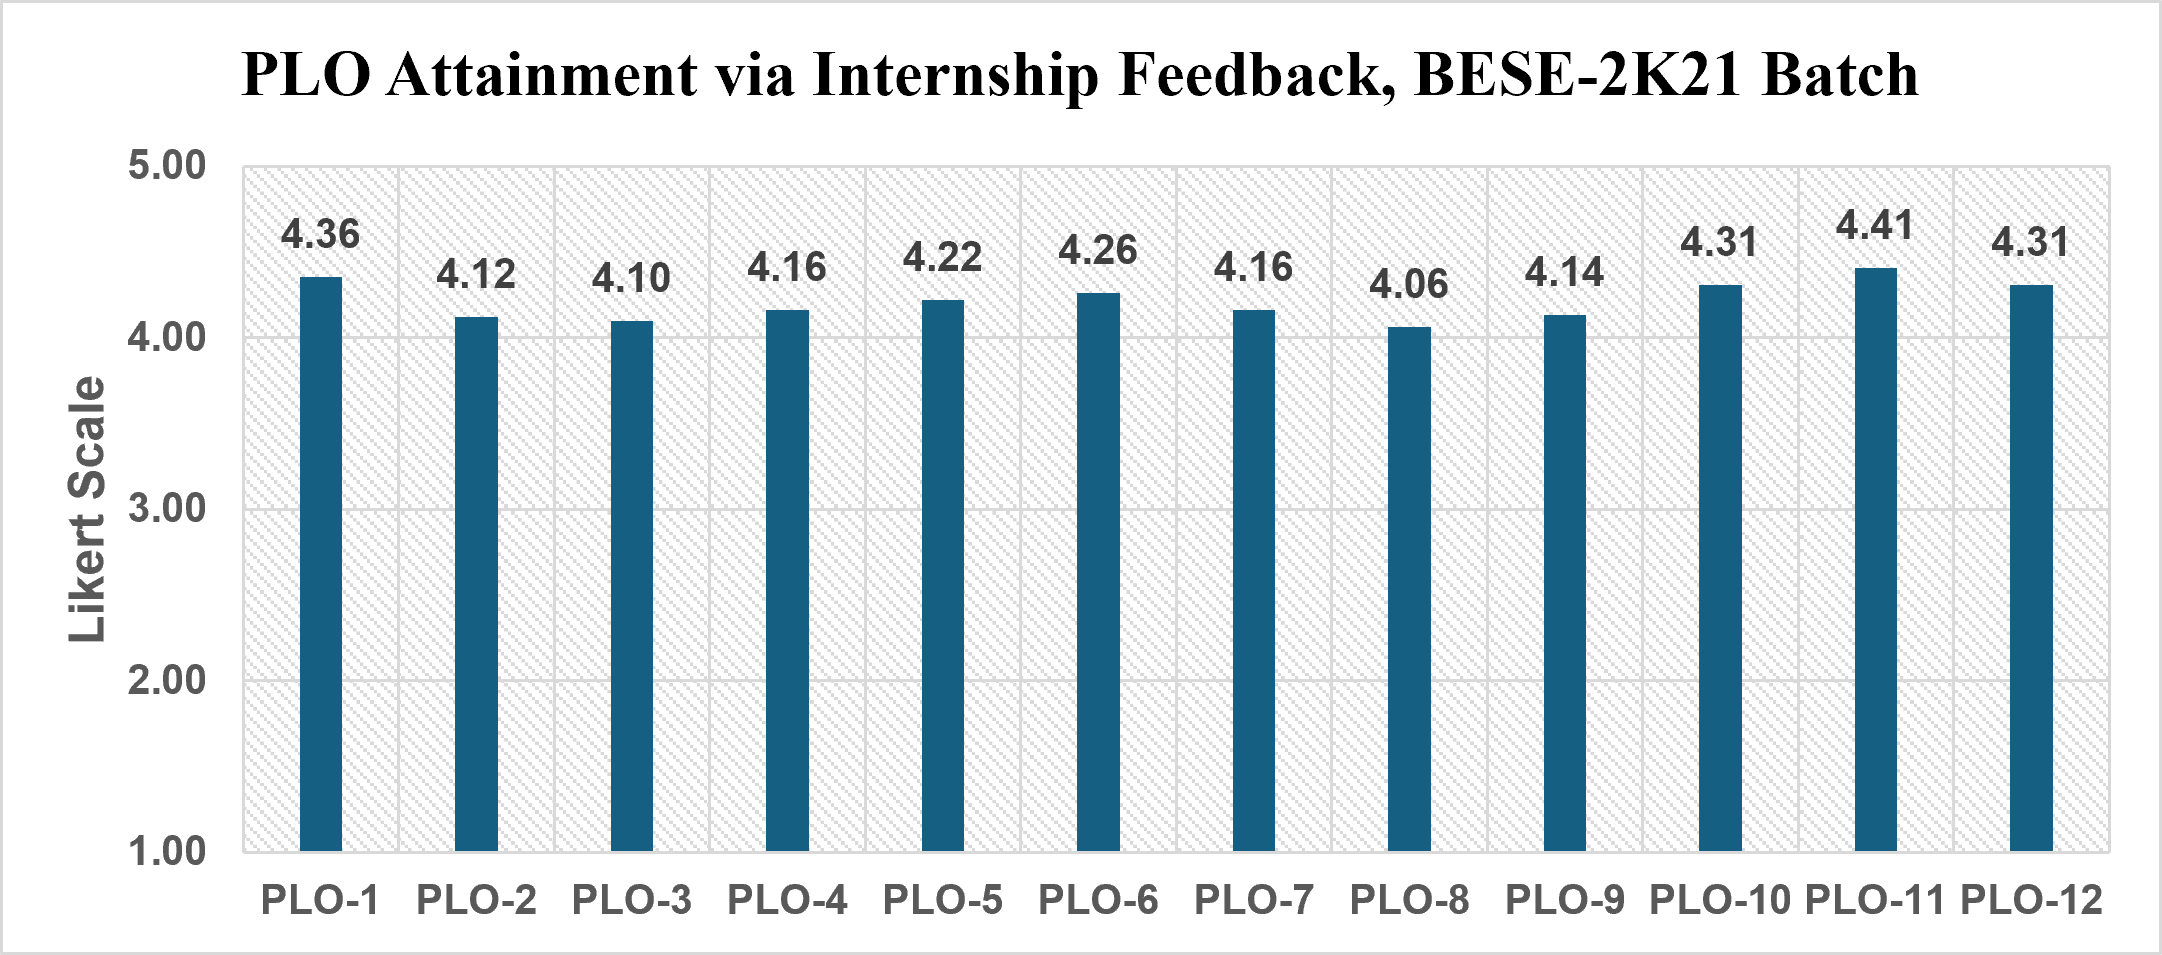
\includegraphics[width=0.90\textwidth]{images/criterion_2/media/image37.png}
\caption{PLO attainment based on internship feedback for the BESE 2K21 Batch.}
\label{figure:PLO attainment based on internship 2K21}
\end{figure}

\begin{table}[H]
\centering
\caption{Internship Feedback for the Batch 2K21}
\begin{tabular}{>{\centering\arraybackslash}p{0.06\textwidth}
                >{\raggedright\arraybackslash}p{0.5\textwidth}
                >{\centering\arraybackslash}p{0.05\textwidth}
                >{\centering\arraybackslash}p{0.05\textwidth}
                >{\centering\arraybackslash}p{0.05\textwidth}
                >{\centering\arraybackslash}p{0.05\textwidth}
                >{\centering\arraybackslash}p{0.05\textwidth}}
\toprule
\textbf{PLO} & \textbf{Rubric} & \textbf{5} & \textbf{4} & \textbf{3} & \textbf{2} & \textbf{1} \\
\midrule
1  & Ability to apply engineering knowledge to solve tasks given at workplace. & 39 & 32 & 10 & 0 & 0 \\
2  & Ability to identify, analyze and solve engineering problems & 31 & 32 & 15 & 3 & 0 \\
3  & Ability to design and develop systems and solutions for complex engineering problems & 29 & 33 & 17 & 2 & 0 \\
4  & Ability to investigate complex problems using experimental design, data analysis, and information synthesis, to draw valid conclusions. & 30 & 35 & 15 & 1 & 0 \\
5  & Ability to utilize modern engineering and IT tools in practice. & 41 & 22 & 13 & 5 & 0 \\
6  & Ability to understand the impact of engineering solutions and their ability to operate effectively in multi-disciplinary environments. & 32 & 38 & 11 & 0 & 0 \\
7  & Ability to understand environmental and sustainability issues and assess the impact of engineering solutions on them & 34 & 27 & 19 & 1 & 0 \\
8  & Professional, reliable and punctual in meeting commitments and deadlines at work. & 31 & 27 & 20 & 3 & 0 \\
9  & Ability to function effectively as an individual, and as a member or leader in diverse teams. & 35 & 27 & 14 & 5 & 0 \\
10 & Ability to create effective documentation, deliver impactful presentations, and handle instructions carefully & 37 & 32 & 12 & 0 & 0 \\
11 & Ability to apply management and decision-making skills for assigned tasks & 46 & 23 & 11 & 1 & 0 \\
12 & Demonstrate interest in work, and acceptance of constructive criticism, feedback and learn from it. & 43 & 24 & 10 & 4 & 0 \\
\bottomrule
\end{tabular}
\label{table:PLO attainment based on internship 2K21}
\end{table}

\textbf{2.\ Batch 2K22 Analysis}

Batch 2K22 sustained high levels of satisfaction, showing slight shifts in technical versus behavioral performance. Figure~\ref{figure:PLO attainment based on internship 2K22} shows the average PLO attainment plots for the BESE 2K22 batch. Table~\ref{table:PLO attainment based on internship 2K22} shows the number of employer responses obtained for each rubric.

\begin{itemize}
\item \textbf{Highest Attainment:} \textbf{PLO 12} (Interest in work and feedback; 49 scores of 5) and \textbf{PLO 1} (Applying engineering knowledge; 47 scores of 5). Employers found these students highly motivated and technically grounded right at the workplace entry level.
\item \textbf{Areas for Growth:} \textbf{PLO 8} (Professionalism, reliability, and punctuality) scored the lowest in the top tier (only 26 scores of 5), though it was heavily compensated by 39 scores of 4. \textbf{PLO 2} (Problem identification and analysis) also showed a higher volume of moderate ratings (20 scores of 3).
\end{itemize}

\begin{figure}[H]
\centering
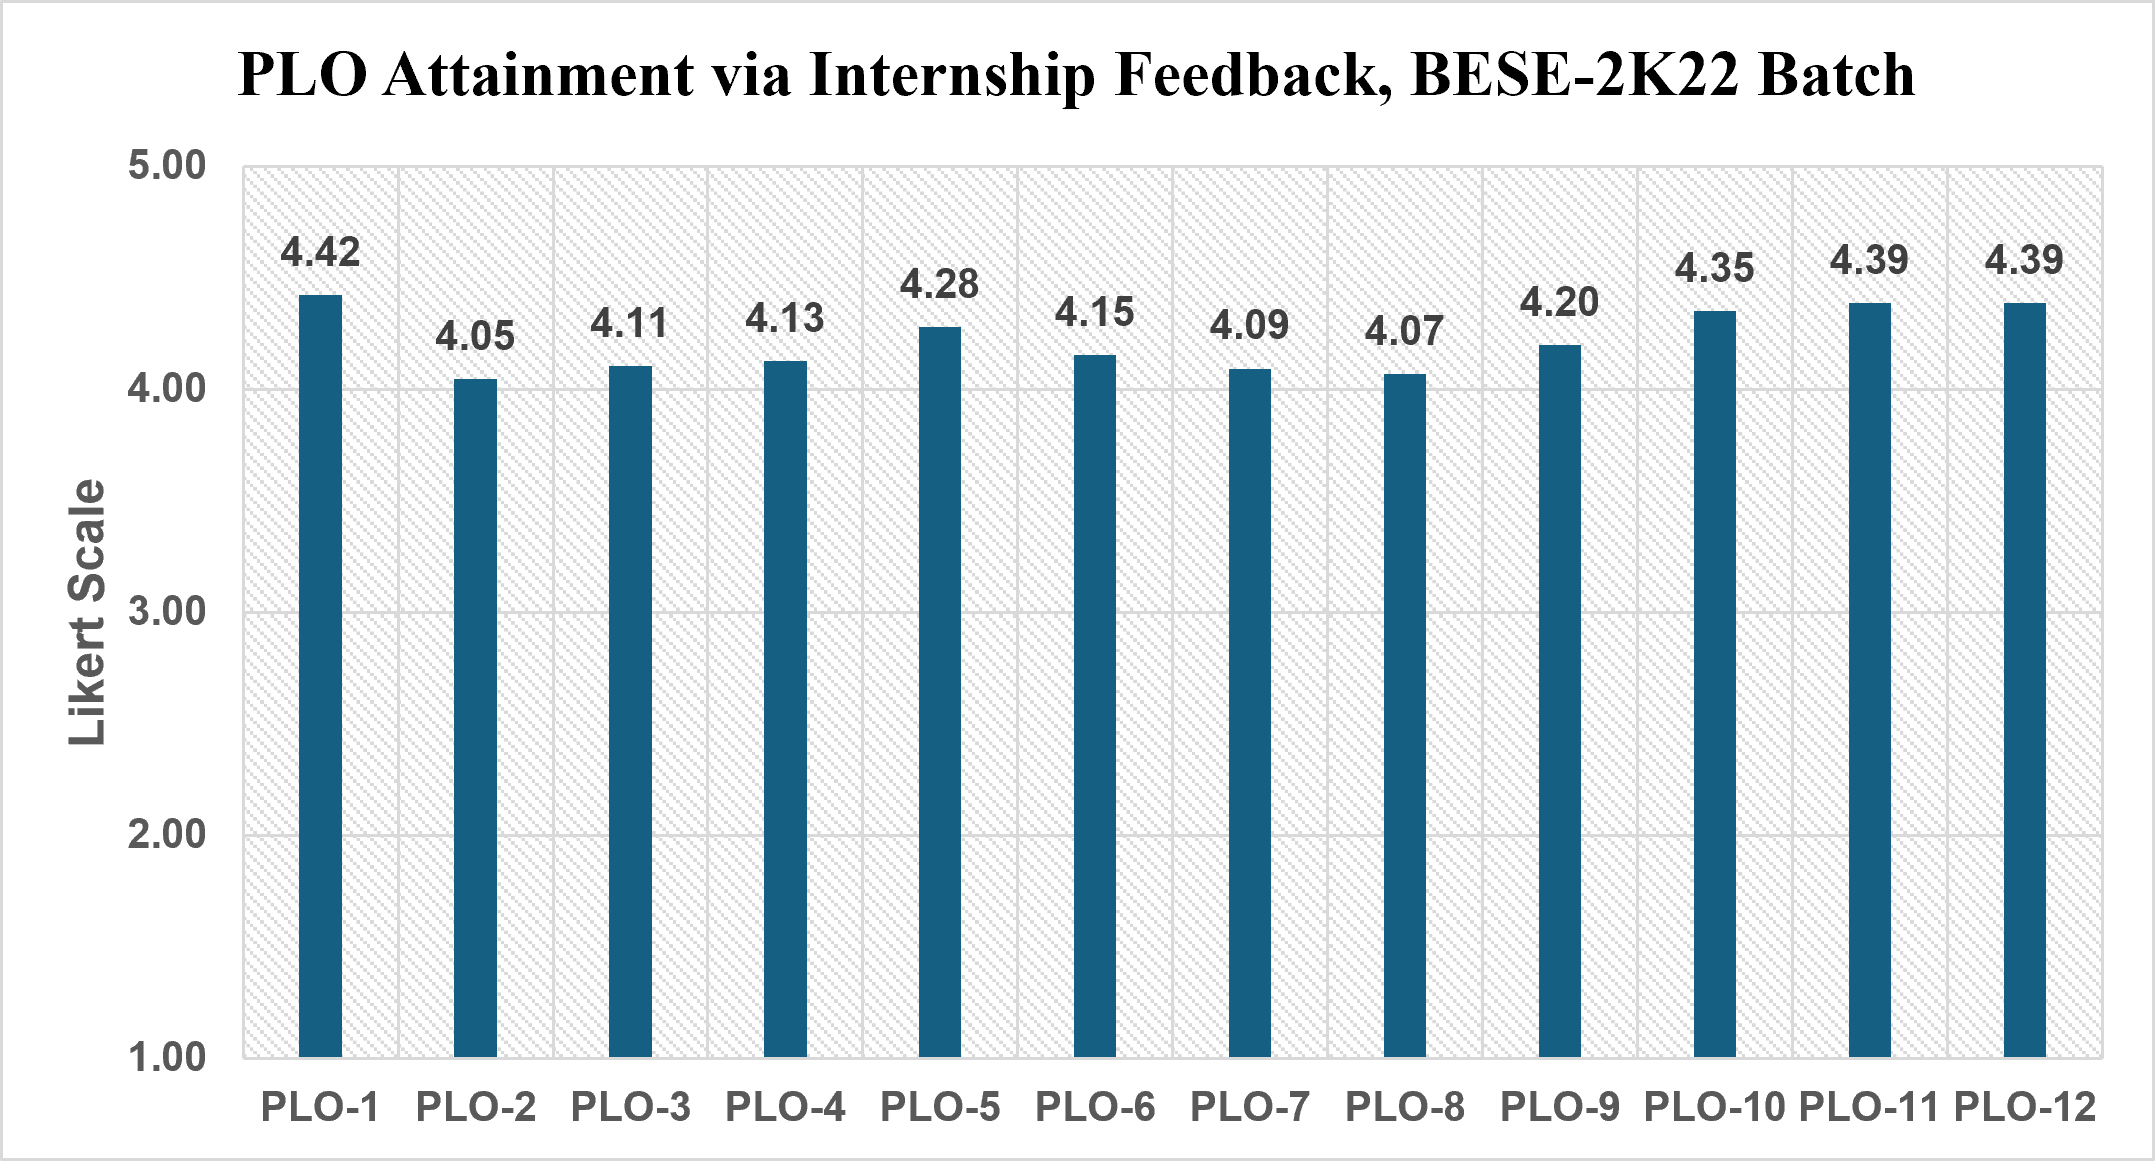
\includegraphics[width=0.90\textwidth]{images/criterion_2/media/image38.png}
\caption{PLO attainment based on internship feedback for the BESE 2K22 Batch.}
\label{figure:PLO attainment based on internship 2K22}
\end{figure}

\begin{longtable}{>{\centering\arraybackslash}p{0.06\textwidth}
                  >{\raggedright\arraybackslash}p{0.5\textwidth}
                  >{\centering\arraybackslash}p{0.05\textwidth}
                  >{\centering\arraybackslash}p{0.05\textwidth}
                  >{\centering\arraybackslash}p{0.05\textwidth}
                  >{\centering\arraybackslash}p{0.05\textwidth}
                  >{\centering\arraybackslash}p{0.05\textwidth}}

\caption{Internship Feedback for the Batch 2K22}
\label{table:PLO attainment based on internship 2K22} \\

\toprule
\textbf{PLO} & \textbf{Rubric} & \textbf{5} & \textbf{4} &
\textbf{3} & \textbf{2} & \textbf{1} \\
\midrule
\endfirsthead

\multicolumn{7}{c}%
{\tablename\ \thetable{} -- continued from previous page} \\
\toprule
\textbf{PLO} & \textbf{Rubric} & \textbf{5} & \textbf{4} &
\textbf{3} & \textbf{2} & \textbf{1} \\
\midrule
\endhead

\midrule
\multicolumn{7}{r}{Continued on next page} \\
\endfoot

\bottomrule
\endlastfoot

1  & Ability to apply engineering knowledge to solve tasks given at workplace. & 47 & 27 & 11 & 0 & 0 \\
2  & Ability to identify, analyze and solve engineering problems & 28 & 35 & 20 & 2 & 0 \\
3  & Ability to design and develop systems and solutions for complex engineering problems & 33 & 29 & 22 & 1 & 0 \\
4  & Ability to investigate complex problems using experimental design, data analysis, and information synthesis, to draw valid conclusions. & 29 & 40 & 14 & 2 & 0 \\
5  & Ability to utilize modern engineering and IT tools in practice. & 40 & 33 & 8 & 4 & 0 \\
6  & Ability to understand the impact of engineering solutions and their ability to operate effectively in multi-disciplinary environments. & 31 & 38 & 14 & 2 & 0 \\
7  & Ability to understand environmental and sustainability issues and assess the impact of engineering solutions on them & 32 & 30 & 22 & 1 & 0 \\
8  & Professional, reliable and punctual in meeting commitments and deadlines at work. & 26 & 39 & 20 & 0 & 0 \\
9  & Ability to function effectively as an individual, and as a member or leader in diverse teams. & 36 & 31 & 17 & 1 & 0 \\
10 & Ability to create effective documentation, deliver impactful presentations, and handle instructions carefully & 45 & 25 & 15 & 0 & 0 \\
11 & Ability to apply management and decision-making skills for assigned tasks & 46 & 27 & 11 & 1 & 0 \\
12 & Demonstrate interest in work, and acceptance of constructive criticism, feedback and learn from it. & 49 & 23 & 11 & 1 & 1 \\

\end{longtable}

\textbf{3.\ Batch 2K23 Analysis}

While the data pool for 2K23 is smaller (interim data), the trend remains consistently positive, skewed heavily toward scores of 4 and 5. Figure~\ref{figure:PLO attainment based on internship 2K23} shows the average PLO attainment plots for the BESE 2K23 batch. Table~\ref{table:PLO attainment based on internship 2K23} shows the number of employer responses obtained for each rubric.

\begin{itemize}
\item \textbf{Highest Attainment:} \textbf{PLO 1} (Applying engineering knowledge), \textbf{PLO 11} (Management/decision-making), and \textbf{PLO 12} (Interest in work/feedback) all tied with 19 scores of 5 out of 24.
\item \textbf{Areas for Growth:} \textbf{PLO 7} (Environmental and sustainability issues) was noticeably weaker in top-tier performance, receiving only 8 scores of 5, though it was balanced by 14 scores of 4.
\end{itemize}

\begin{figure}[H]
\centering
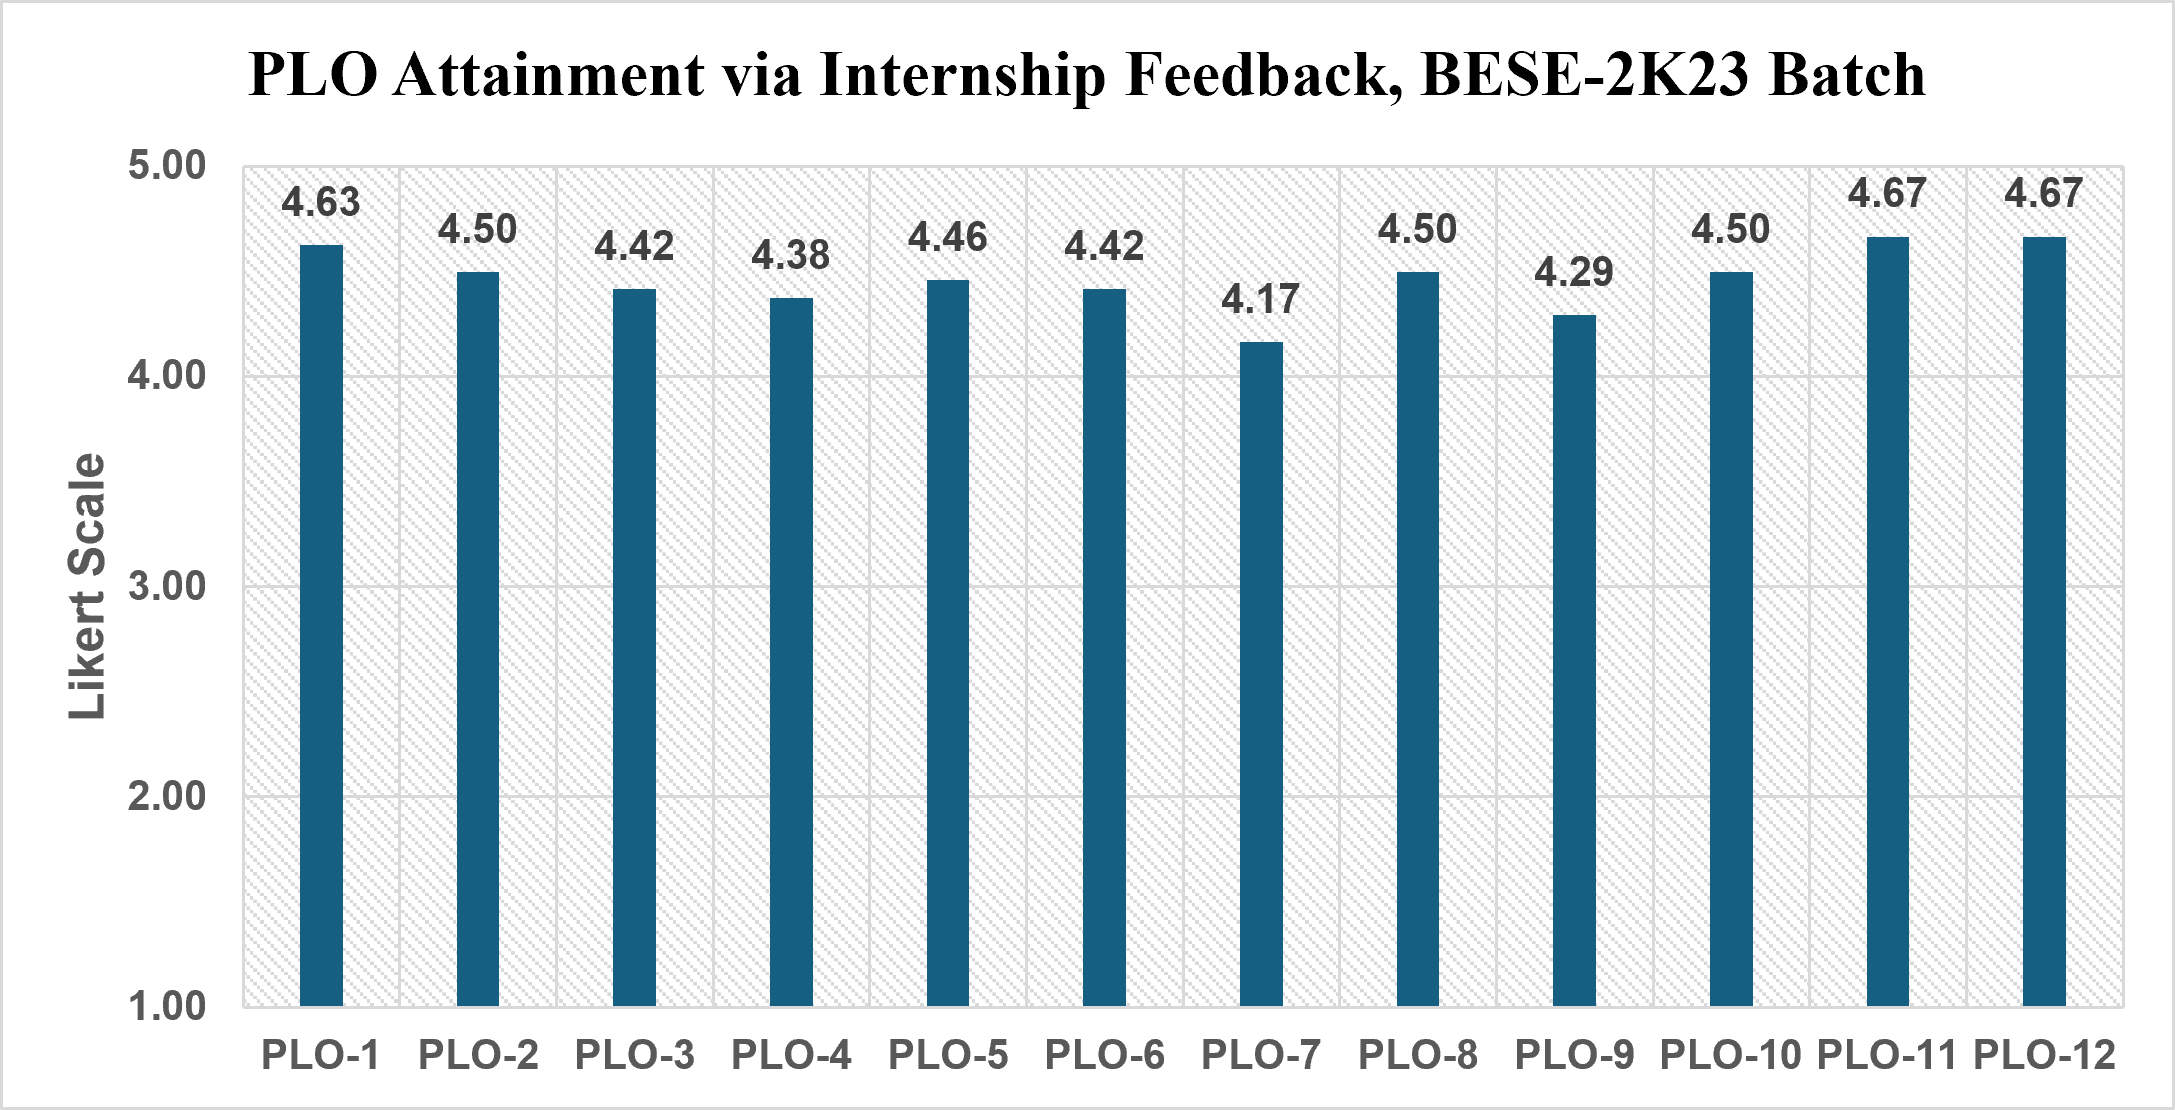
\includegraphics[width=0.90\textwidth]{images/criterion_2/media/image39.png}
\caption{PLO attainment based on internship feedback for the BESE 2K23 Batch.}
\label{figure:PLO attainment based on internship 2K23}
\end{figure}

\begin{table}[H]
\centering
\caption{Internship Feedback for the Batch 2K23}
\begin{tabular}{>{\centering\arraybackslash}p{0.06\textwidth}
                >{\raggedright\arraybackslash}p{0.5\textwidth}
                >{\centering\arraybackslash}p{0.05\textwidth}
                >{\centering\arraybackslash}p{0.05\textwidth}
                >{\centering\arraybackslash}p{0.05\textwidth}
                >{\centering\arraybackslash}p{0.05\textwidth}
                >{\centering\arraybackslash}p{0.05\textwidth}}
\toprule
\textbf{PLO} & \textbf{Rubric} & \textbf{5} & \textbf{4} & \textbf{3} & \textbf{2} & \textbf{1} \\
\midrule
1  & Ability to apply engineering knowledge to solve tasks given at workplace. & 19 & 3 & 1 & 0 & 1 \\
2  & Ability to identify, analyze and solve engineering problems & 16 & 6 & 1 & 0 & 1 \\
3  & Ability to design and develop systems and solutions for complex engineering problems & 14 & 8 & 1 & 0 & 1 \\
4  & Ability to investigate complex problems using experimental design, data analysis, and information synthesis, to draw valid conclusions. & 13 & 9 & 1 & 0 & 1 \\
5  & Ability to utilize modern engineering and IT tools in practice. & 15 & 7 & 1 & 0 & 1 \\
6  & Ability to understand the impact of engineering solutions and their ability to operate effectively in multi-disciplinary environments. & 15 & 6 & 2 & 0 & 1 \\
7  & Ability to understand environmental and sustainability issues and assess the impact of engineering solutions on them & 8 & 14 & 1 & 0 & 1 \\
8  & Professional, reliable and punctual in meeting commitments and deadlines at work. & 16 & 6 & 1 & 0 & 1 \\
9  & Ability to function effectively as an individual, and as a member or leader in diverse teams. & 14 & 5 & 4 & 0 & 1 \\
10 & Ability to create effective documentation, deliver impactful presentations, and handle instructions carefully & 16 & 6 & 1 & 0 & 1 \\
11 & Ability to apply management and decision-making skills for assigned tasks & 19 & 4 & 0 & 0 & 1 \\
12 & Demonstrate interest in work, and acceptance of constructive criticism, feedback and learn from it. & 19 & 4 & 0 & 0 & 1 \\
\bottomrule
\end{tabular}
\label{table:PLO attainment based on internship 2K23}
\end{table}

\textbf{Comparative PLO Performance Matrix}

To easily spot macro trends, the Table~\ref{table: Comparative PLO Performance Matrix} highlights the percentage of Excellent to Very Good ratings (Scores 4 \& 5 combined) for each PLO across the three cohorts:

\begin{table}[H]
\footnotesize
\centering
\caption{Comparative PLO Performance Matrix -- Internship Feedback (Scores 4 \& 5 Combined)}
\label{table: Comparative PLO Performance Matrix}
\begin{tabular}{>{\centering\arraybackslash}p{0.09\textwidth}
                >{\raggedright\arraybackslash}p{0.36\textwidth}
                >{\centering\arraybackslash}p{0.15\textwidth}
                >{\centering\arraybackslash}p{0.15\textwidth}
                >{\centering\arraybackslash}p{0.15\textwidth}}
\toprule
\textbf{PLOs} & \textbf{Rubric Summary} & \textbf{Batch 2K21} & \textbf{Batch 2K22} & \textbf{Batch 2K23} \\
\midrule
PLO 1  & Engineering Knowledge         & 87.7\% & 87.1\% & 91.7\% \\
PLO 2  & Problem Analysis        & 77.8\% & 74.1\% & 91.7\% \\
PLO 3  & Design \& Development of Solutions             & 76.5\% & 72.9\% & 91.7\% \\
PLO 4  & Investigation         & 80.2\% & 81.2\% & 91.7\% \\
PLO 5  & Modern Tool Usage (IT/Engineering)        & 77.8\% & 85.9\% & 91.7\% \\
PLO 6  & The Engineer \& Society & 86.4\% & 81.2\% & 87.5\% \\
PLO 7  & Environment \& Sustainability             & 75.3\% & 72.9\% & 91.7\% \\
PLO 8  & Ethics                                    & 71.6\% & 76.5\% & 91.7\% \\
PLO 9  & Individual \& Team Work                   & 76.5\% & 78.8\% & 79.2\% \\
PLO 10 & Communication Skills            & 85.2\% & 82.4\% & 91.7\% \\
PLO 11 & Project Management                        & 85.2\% & 85.9\% & 95.8\% \\
PLO 12 & Lifelong Learning                         & 82.7\% & 84.7\% & 95.8\% \\
\bottomrule
\end{tabular}
\end{table}

\textbf{Key Observations}

\begin{itemize}
\item \textbf{Consistently Strong Core Competencies:} Across all three batches, \textbf{PLO 1} (Engineering Knowledge), \textbf{PLO 11} (Management/Decision-making), and \textbf{PLO 12} (Lifelong learning/Attitude) are the highest performing areas. Employers consistently note that BESE students have an excellent work ethic, are receptive to constructive criticism, and grasp foundational engineering concepts quickly.
\item \textbf{The ``Complex Engineering'' Bottleneck:} In both 2K21 and 2K22, \textbf{PLO 2} (Problem Analysis) and \textbf{PLO 3} (Design/Development of Solutions) experience a noticeable dip in ``5'' scores, moving into ``4'' and ``3'' ranges. This indicates that while students are capable, executing complex architecture designs or deep systemic troubleshooting in a live corporate environment remains their steepest learning curve.
\item \textbf{Modern Tool Progress:} There is a positive trajectory in \textbf{PLO 5} (Modern Tool Usage), rising from 77.8\% (2K21) to 85.9\% (2K22) in top-tier positive reviews. This suggests that academic curriculum adjustments or lab tools are aligning better with current industry stacks.
\item \textbf{Professionalism \& Teamwork Stabilization:} \textbf{PLO 8} (Punctuality/Commitment) and \textbf{PLO 9} (Teamwork) score slightly lower on absolute ``Excellent'' marks but hold a strong ``Good/Satisfactory'' baseline. This is normal for interns transitioning from a flexible academic environment to rigid corporate schedules.
\end{itemize}

\section{Graduate Exit Survey Form}
\label{annex:graduate-exit-survey-form}
\includefullannexure{appendices/criterion_2/Graduate Exit Form.pdf}


\clearpage
\section{Graduate Exit Survey Analysis}
\label{annex:graduate-exit-survey-analysis}

This annexure evaluates the Program Learning Outcomes (PLOs) attainment for the BESE program based on the Graduate Exit Survey. The survey captures the graduating students' self-assessment of their engineering knowledge, technical skills, and professional attributes on a 5-point Likert scale.

\subsection{Batch 2K20 Analysis}

The graduating batch of 2K20 established a highly stable and balanced baseline across all engineering criteria, with all mean scores residing within a tight, healthy band of \textbf{3.91 to 4.15} as shown in Figure~\ref{fig:exit-survey-2k20} and Table~\ref{table:PLO attainment based on the Graduate Exit}.

\begin{itemize}
\item \textbf{Key Strengths:} Students felt most confident in their preparation for \textbf{Lifelong Learning (PLO 12: 4.15)} and their \textbf{Ethics (PLO 8: 4.11)}.
\item \textbf{Areas of Relative Moderation:} The lowest score, though still highly positive, was in \textbf{Engineering Knowledge (PLO 1: 3.91)}.
\end{itemize}

\begin{figure}[H]
\centering
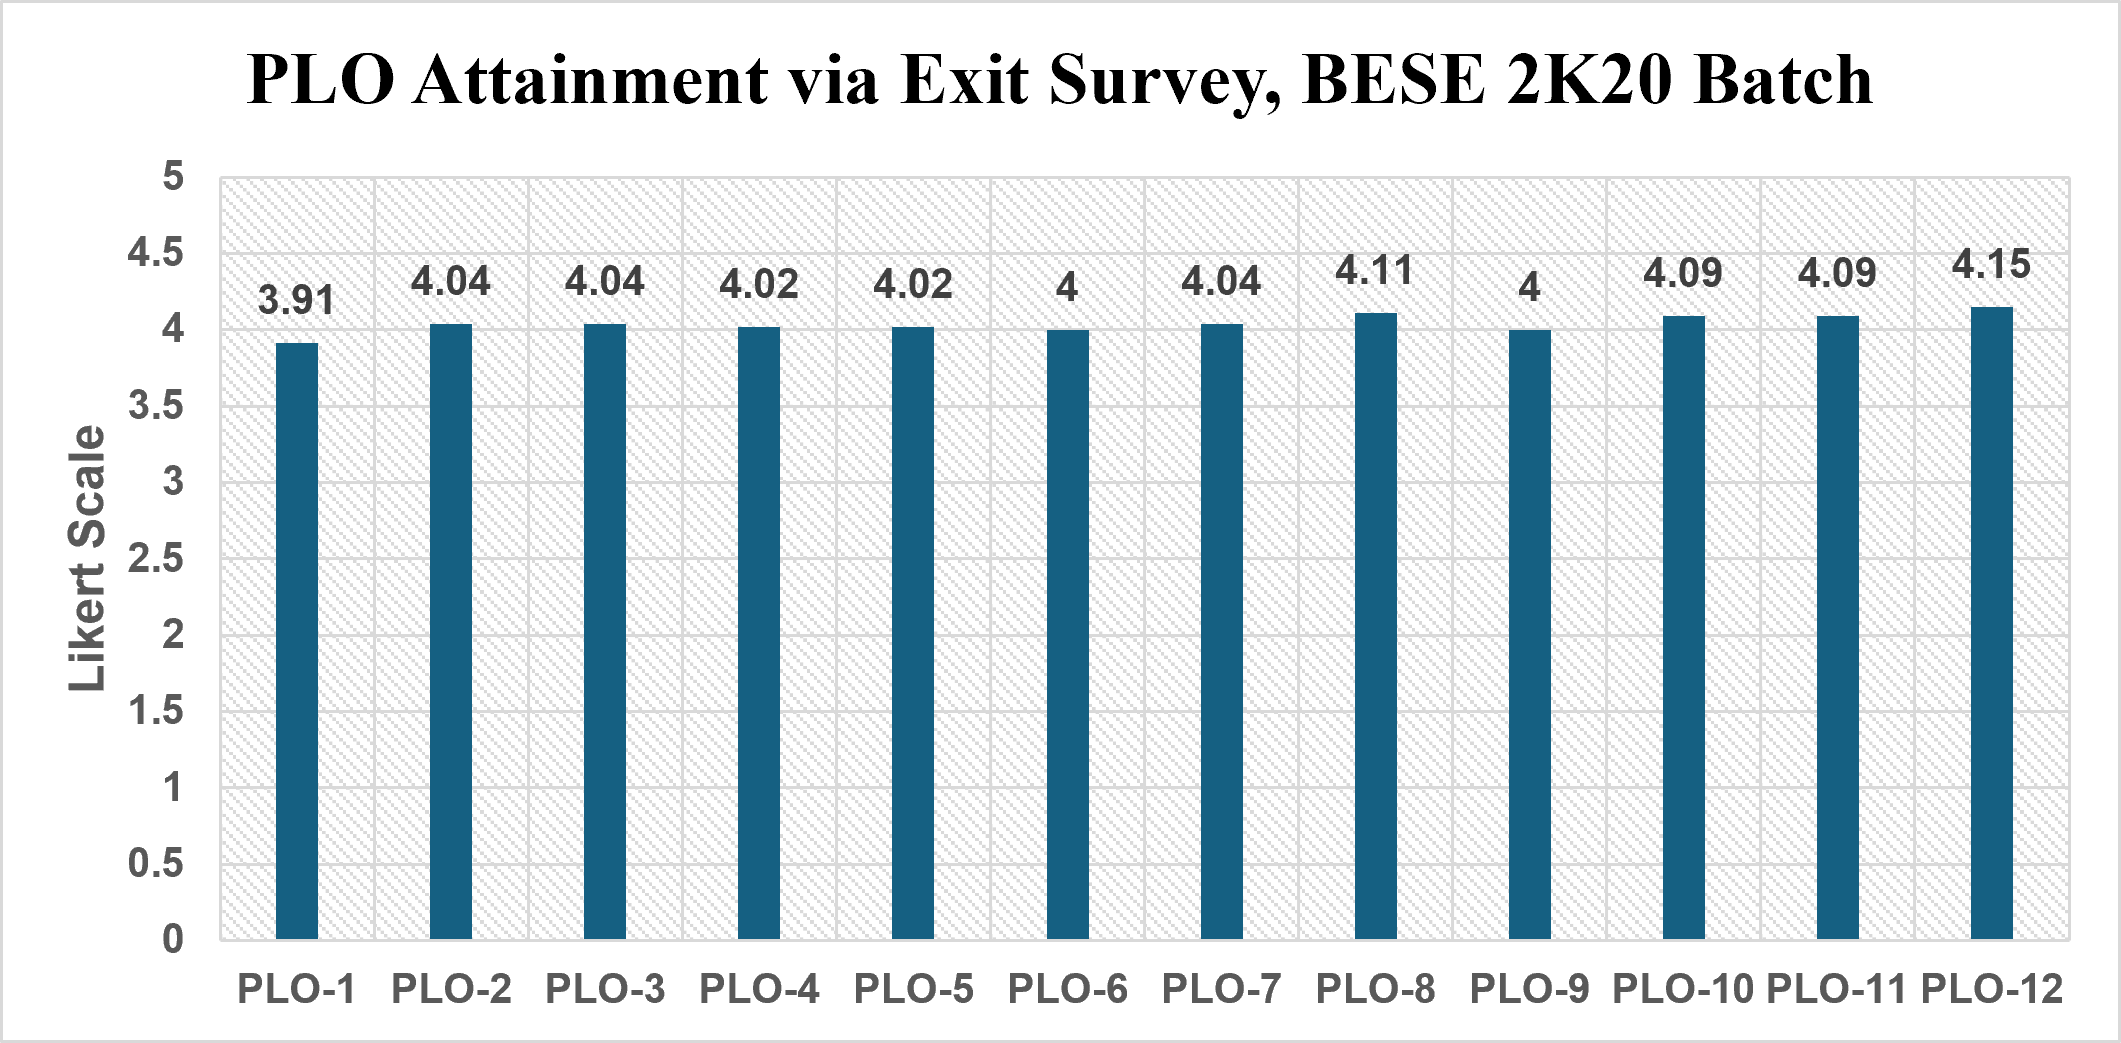
\includegraphics[width=0.90\textwidth]{images/criterion_2/media/image40.png}
\caption{PLO attainment based on the Graduate Exit Survey for the BESE 2K20 Batch.}
\label{fig:exit-survey-2k20}
\end{figure}

\begin{longtable}{>{\centering\arraybackslash}p{0.08\textwidth}
                  >{\raggedright\arraybackslash}p{0.74\textwidth}
                  >{\centering\arraybackslash}p{0.09\textwidth}}

\caption{Result of Exit Survey for the Batch 2K20}
\label{table:PLO attainment based on the Graduate Exit} \\

\toprule
\textbf{PLO} & \textbf{Question} & \textbf{Score} \\
\midrule
\endfirsthead

\multicolumn{3}{c}{\tablename\ \thetable{} -- continued from previous page} \\
\toprule
\textbf{PLO} & \textbf{Question} & \textbf{Score} \\
\midrule
\endhead

\midrule
\multicolumn{3}{r}{Continued on next page} \\
\endfoot

\bottomrule
\endlastfoot

PLO 1  & My engineering education has developed the knowledge and skills I will need for my future career. & 3.91 \\
PLO 2  & I can analyze engineering problems using fundamental principles of mathematics, science, and engineering. & 4.04 \\
PLO 3  & I have acquired the ability to analyze and develop solutions for complex, real-world engineering problems involving multiple constraints and stakeholders. & 4.04 \\
PLO 4  & I can independently design experiments, analyze and interpret data, and synthesize findings to draw valid conclusions. & 4.02 \\
PLO 5  & I can select and effectively use the latest tools employed in the engineering industry. & 4.02 \\
PLO 6  & I am able to assess societal, health, safety, legal and cultural implications and the consequent responsibilities relevant to professional engineering practices. & 4.00 \\
PLO 7  & I am able to understand the societal and environmental impacts of engineering solutions and recognize the importance of sustainable development. & 4.04 \\
PLO 8  & I consider ethical principles in my engineering practice and take responsibility for the outcomes of my decisions. & 4.11 \\
PLO 9  & I can work effectively both independently and as part of a team on projects that involve collaboration across diverse technical and non-technical fields. & 4.00 \\
PLO 10 & I can express technical concepts through reports, presentations, and discussions with both technical and non-technical audiences. & 4.09 \\
PLO 11 & I am able to apply engineering and management skills to contribute to or lead projects in multidisciplinary teams. & 4.09 \\
PLO 12 & I have the ability to recognize the importance of and pursue lifelong learning in the broader context of innovation and technological developments. & 4.15 \\

\end{longtable}

\subsection{Batch 2K21 Analysis}

The 2K21 batch showed a slight improvement in self-assessed confidence levels across core engineering competencies compared to 2K20, with scores spanning a range of \textbf{3.87 to 4.21} as shown in Figure~\ref{fig:exit-survey-2k21} and Table~\ref{table:exit-survey-2k21}.

\begin{itemize}
\item \textbf{Key Strengths:} Non-technical and professional attributes remained the strongest pillars. \textbf{Communication (PLO 10: 4.21)}, \textbf{Ethics (PLO 8: 4.20)}, and \textbf{Individual \& Team Work (PLO 9: 4.20)} were the top-rated outcomes.
\item \textbf{Areas of Relative Moderation:} \textbf{Modern Tool Usage (PLO 5: 3.87)} and \textbf{Engineering Knowledge (PLO 1: 3.99)} were the lowest across the dataset for this batch.
\end{itemize}

\begin{figure}[H]
\centering
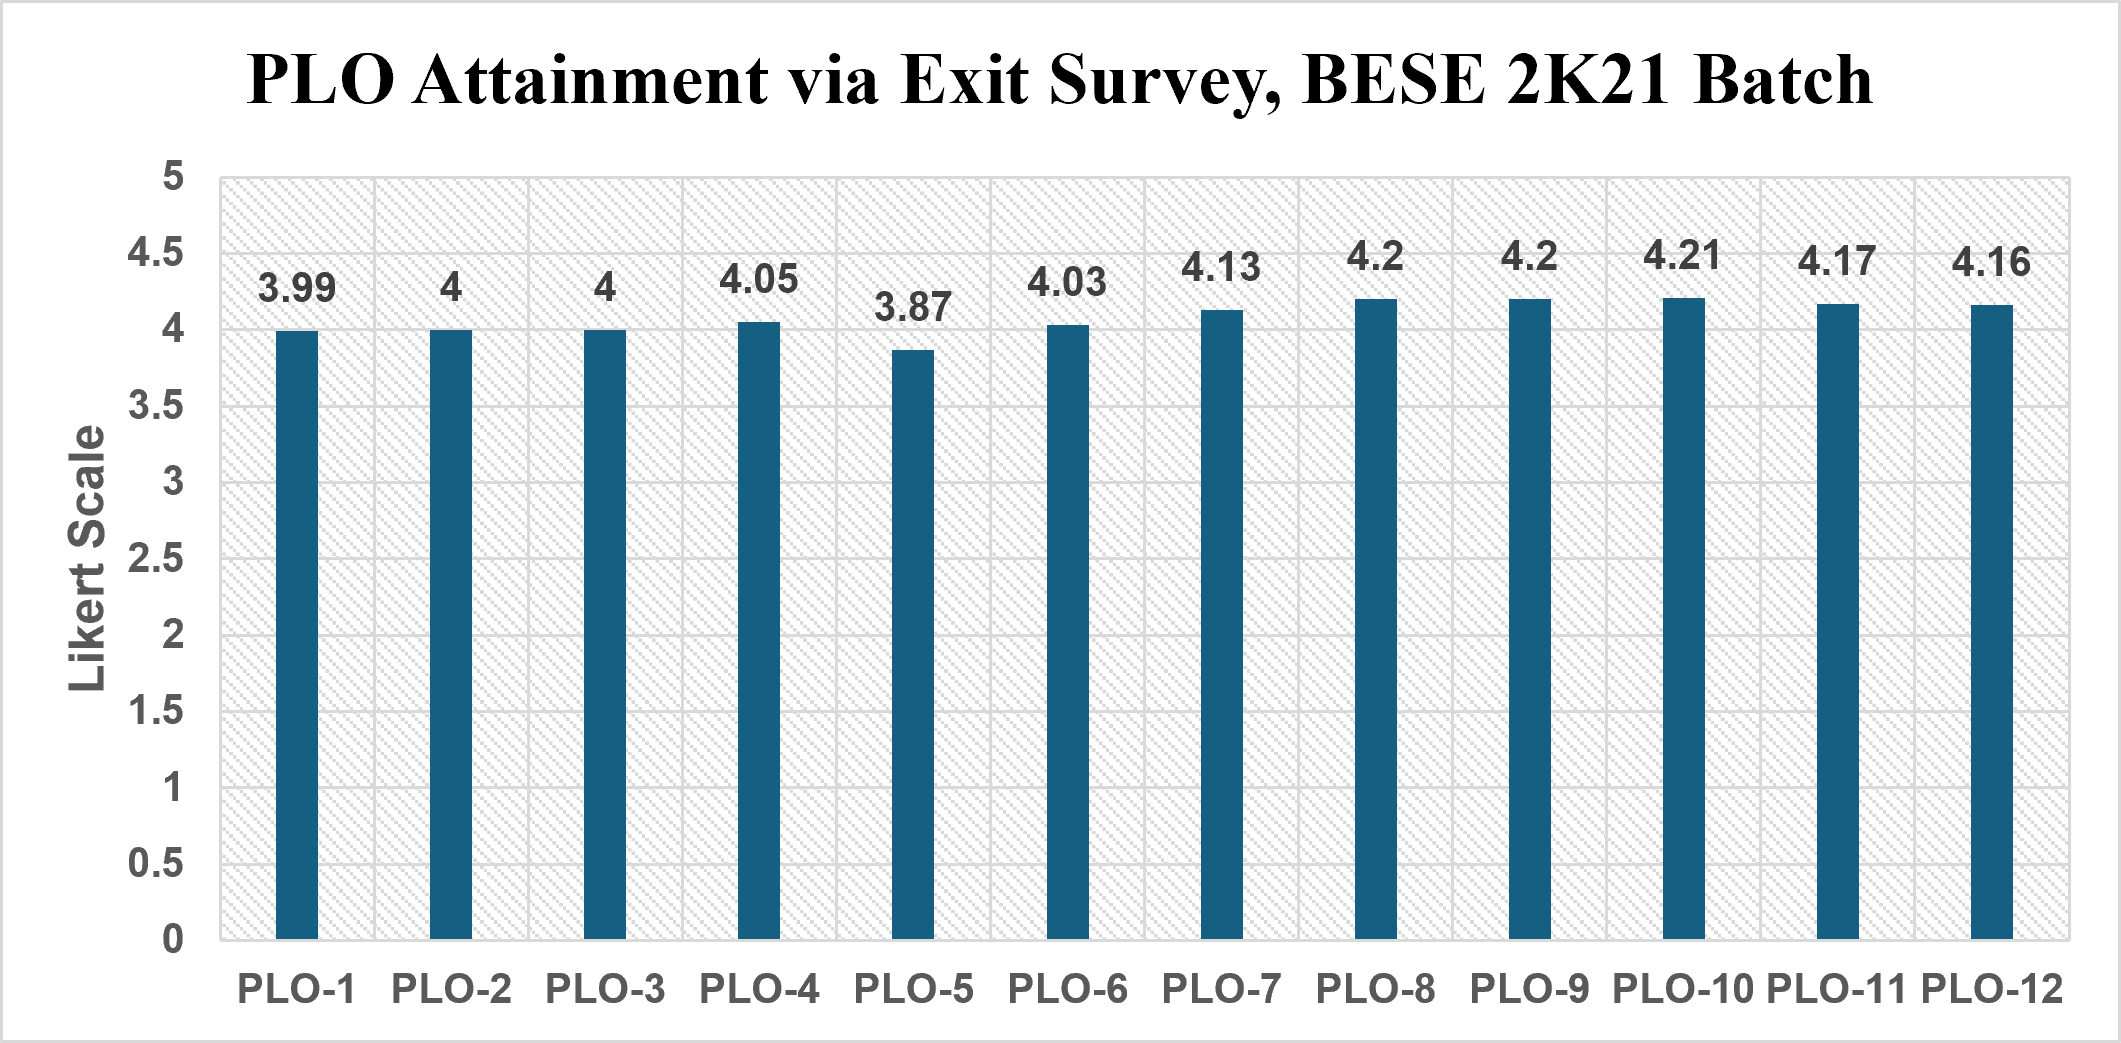
\includegraphics[width=0.90\textwidth]{images/criterion_2/media/image41.png}
\caption{PLO attainment based on the Graduate Exit Survey for the BESE 2K21 Batch.}
\label{fig:exit-survey-2k21}
\end{figure}


\begin{longtable}{>{\centering\arraybackslash}p{0.08\textwidth}
                  >{\raggedright\arraybackslash}p{0.74\textwidth}
                  >{\centering\arraybackslash}p{0.09\textwidth}}

\caption{Result of Exit Survey for the Batch 2K21}
\label{table:exit-survey-2k21} \\

\toprule
\textbf{PLO} & \textbf{Question} & \textbf{Score} \\
\midrule
\endfirsthead

\multicolumn{3}{c}{\tablename\ \thetable{} -- continued from previous page} \\
\toprule
\textbf{PLO} & \textbf{Question} & \textbf{Score} \\
\midrule
\endhead

\midrule
\multicolumn{3}{r}{Continued on next page} \\
\endfoot

\bottomrule
\endlastfoot

PLO 1  & My engineering education has developed the knowledge and skills I will need for my future career. & 3.99 \\
PLO 2  & I can analyze engineering problems using fundamental principles of mathematics, science, and engineering. & 4.00 \\
PLO 3  & I have acquired the ability to analyze and develop solutions for complex, real-world engineering problems involving multiple constraints and stakeholders. & 4.00 \\
PLO 4  & I can independently design experiments, analyze and interpret data, and synthesize findings to draw valid conclusions. & 4.05 \\
PLO 5  & I can select and effectively use the latest tools employed in the engineering industry. & 3.87 \\
PLO 6  & I am able to assess societal, health, safety, legal and cultural implications and the consequent responsibilities relevant to professional engineering practices. & 4.03 \\
PLO 7  & I am able to understand the societal and environmental impacts of engineering solutions and recognize the importance of sustainable development. & 4.13 \\
PLO 8  & I consider ethical principles in my engineering practice and take responsibility for the outcomes of my decisions. & 4.20 \\
PLO 9  & I can work effectively both independently and as part of a team on projects that involve collaboration across diverse technical and non-technical fields. & 4.20 \\
PLO 10 & I can express technical concepts through reports, presentations, and discussions with both technical and non-technical audiences. & 4.21 \\
PLO 11 & I am able to apply engineering and management skills to contribute to or lead projects in multidisciplinary teams. & 4.17 \\
PLO 12 & I have the ability to recognize the importance of and pursue lifelong learning in the broader context of innovation and technological developments. & 4.16 \\

\end{longtable}

\subsection{Batch 2K22 Analysis}

As shown in Figure~\ref{fig:exit-survey-2k22} and Table~\ref{table:exit-survey-2k22}, the scores for this 2K22 batch fall within a tight band from \textbf{3.89 to 4.07}, indicating a very honest, grounded, and realistic self-assessment by the graduating students.

\begin{itemize}
\item \textbf{Key Strengths:} The batch excels in interpersonal attributes, showcasing peak confidence in team collaboration across diverse fields (\textbf{PLO 9: 4.07}), effective technical communication (\textbf{PLO 10: 4.02}), and experimental design and data analysis (\textbf{PLO 4: 4.01}).
\item \textbf{Areas for Improvement:} Action is needed to reinforce professional ethics and accountability (\textbf{PLO 8: 3.89}), while incrementally boosting core engineering knowledge foundations (\textbf{PLO 1: 3.94}) and hands-on mastery of evolving industry toolsets (\textbf{PLO 5: 3.95}).
\end{itemize}


\begin{figure}[H]
\centering
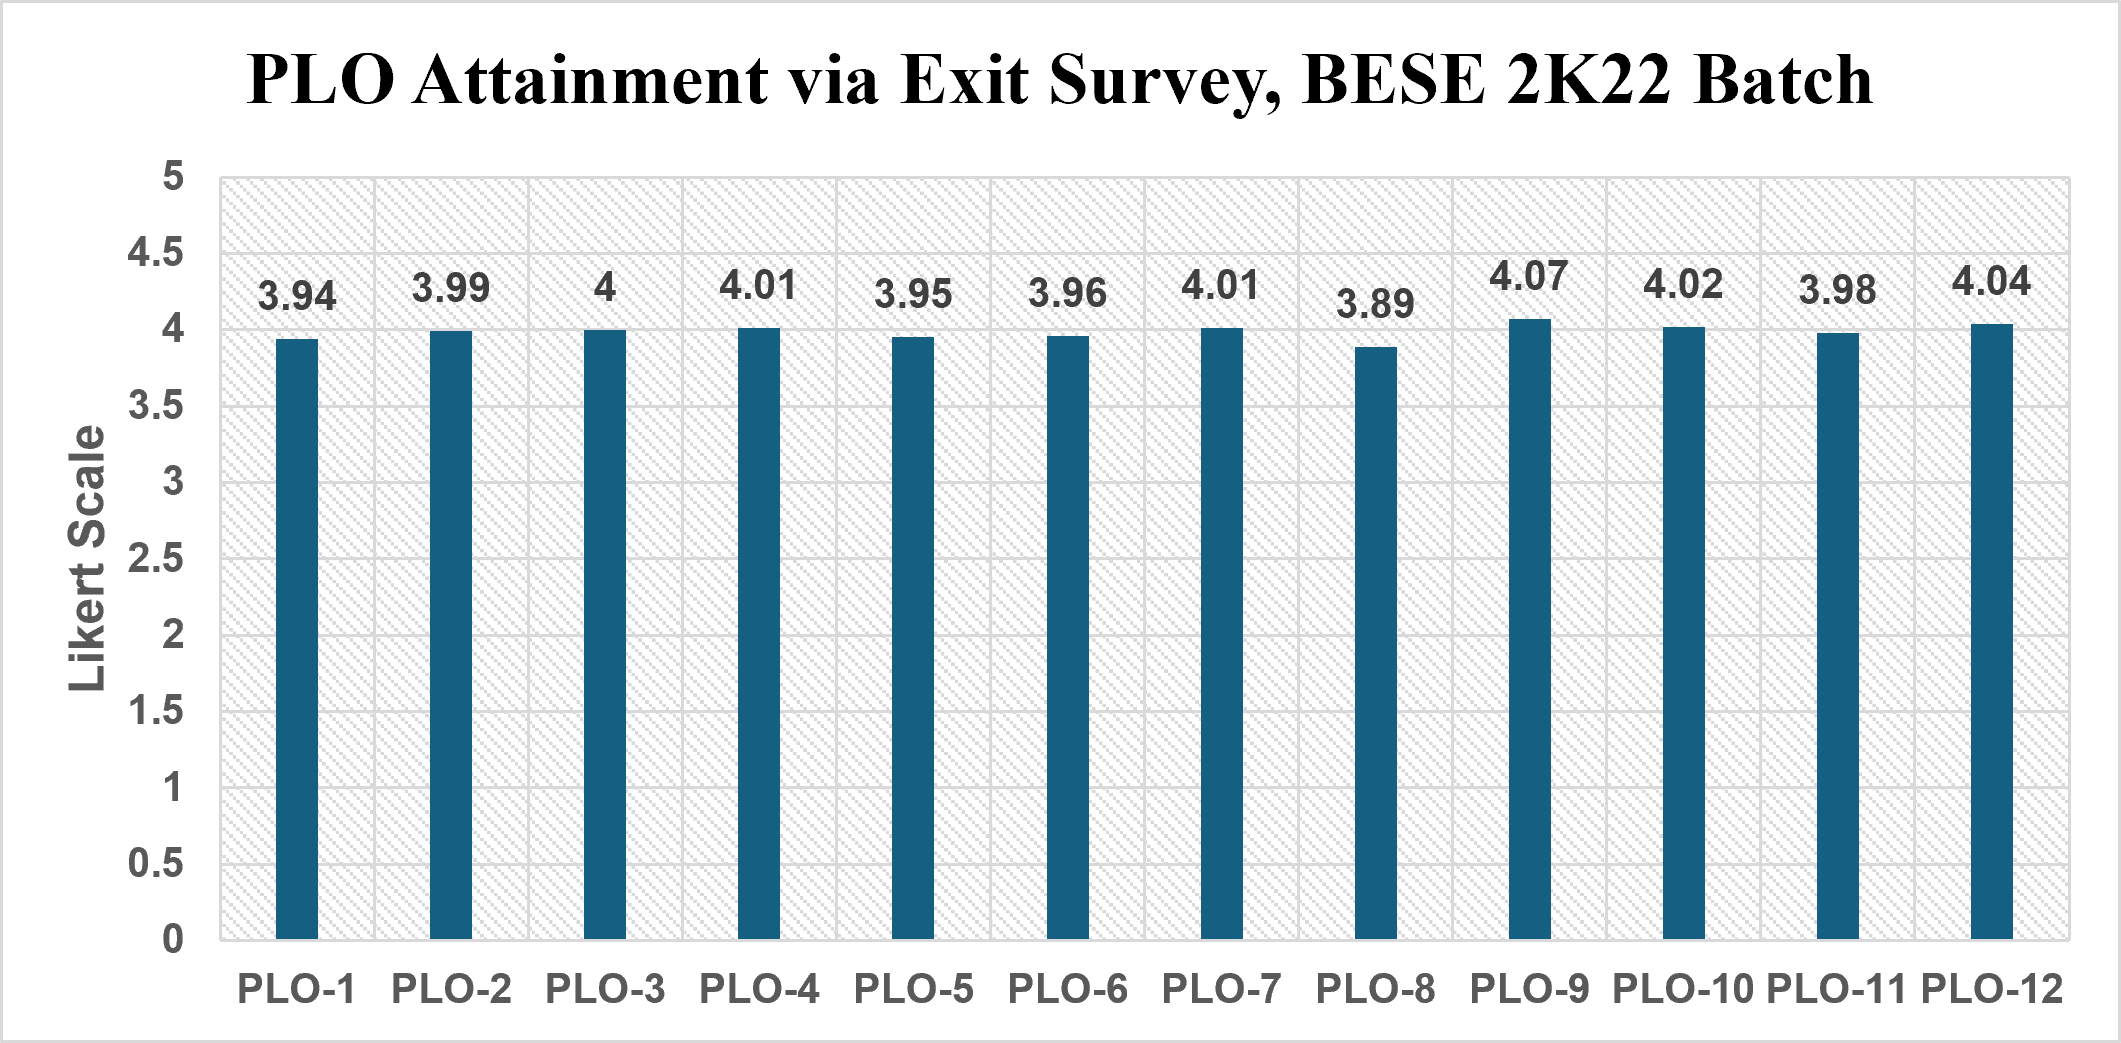
\includegraphics[width=0.90\textwidth]{images/criterion_2/media/image42.png}
\caption{PLO attainment based on the Graduate Exit Survey for the BESE 2K22 Batch.}
\label{fig:exit-survey-2k22}
\end{figure}

\begin{longtable}{>{\centering\arraybackslash}p{0.08\textwidth}
                  >{\raggedright\arraybackslash}p{0.74\textwidth}
                  >{\centering\arraybackslash}p{0.09\textwidth}}

\caption{Result of Exit Survey for the Batch 2K22}
\label{table:exit-survey-2k22} \\

\toprule
\textbf{PLO} & \textbf{Question} & \textbf{Score} \\
\midrule
\endfirsthead

\multicolumn{3}{c}{\tablename\ \thetable{} -- continued from previous page} \\
\toprule
\textbf{PLO} & \textbf{Question} & \textbf{Score} \\
\midrule
\endhead

\midrule
\multicolumn{3}{r}{Continued on next page} \\
\endfoot

\bottomrule
\endlastfoot

PLO 1  & My engineering education has developed the knowledge and skills I will need for my future career. & 3.94 \\
PLO 2  & I can analyze engineering problems using fundamental principles of mathematics, science, and engineering. & 3.99 \\
PLO 3  & I have acquired the ability to analyze and develop solutions for complex, real-world engineering problems involving multiple constraints and stakeholders. & 4.00 \\
PLO 4  & I can independently design experiments, analyze and interpret data, and synthesize findings to draw valid conclusions. & 4.01 \\
PLO 5  & I can select and effectively use the latest tools employed in the engineering industry. & 3.95 \\
PLO 6  & I am able to assess societal, health, safety, legal and cultural implications and the consequent responsibilities relevant to professional engineering practices. & 3.96 \\
PLO 7  & I am able to understand the societal and environmental impacts of engineering solutions and recognize the importance of sustainable development. & 4.01 \\
PLO 8  & I consider ethical principles in my engineering practice and take responsibility for the outcomes of my decisions. & 3.89 \\
PLO 9  & I can work effectively both independently and as part of a team on projects that involve collaboration across diverse technical and non-technical fields. & 4.07 \\
PLO 10 & I can express technical concepts through reports, presentations, and discussions with both technical and non-technical audiences. & 4.02 \\
PLO 11 & I am able to apply engineering and management skills to contribute to or lead projects in multidisciplinary teams. & 3.98 \\
PLO 12 & I have the ability to recognize the importance of and pursue lifelong learning in the broader context of innovation and technological developments. & 4.04 \\

\end{longtable}
\clearpage
\section{Corrective Action Form}
\label{annex:caf}

\begin{figure}[H]
\centering
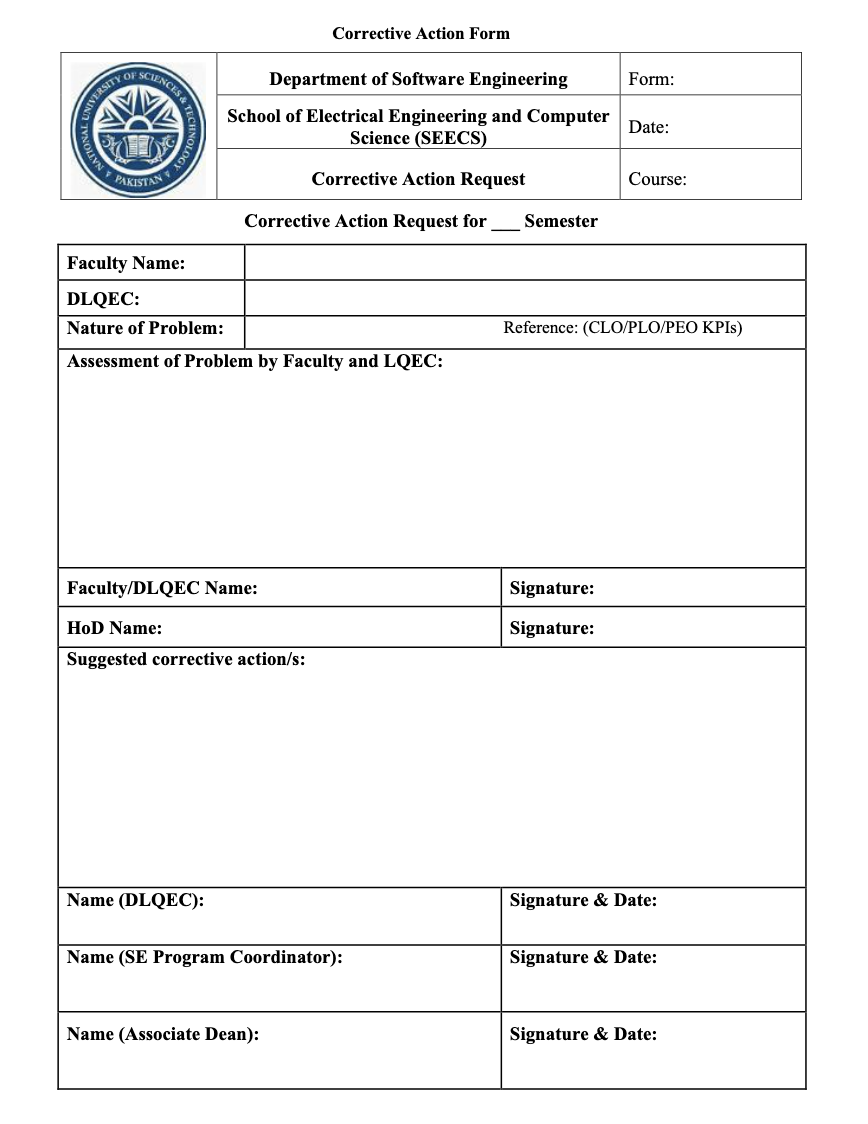
\includegraphics[width=1.0\textwidth]{images/criterion_2/media/corrective.png}
\caption{Corrective Action Form}
\end{figure}
%\includefullannexure{appendices/criterion_2/Corrective Action Form.pdf}

\section{Corrective Action Form  -- OOP}
\label{annex:caf-oop}
\includefullannexure{appendices/criterion_2/CAF_OOP.pdf}

\clearpage
\section{DBS Meeting Minutes}
\label{annex:dbs-mom}
%\includefullannexure{appendices/criterion_2/DBS Meeting Minutes.pdf}
\begin{figure}[H]
\centering
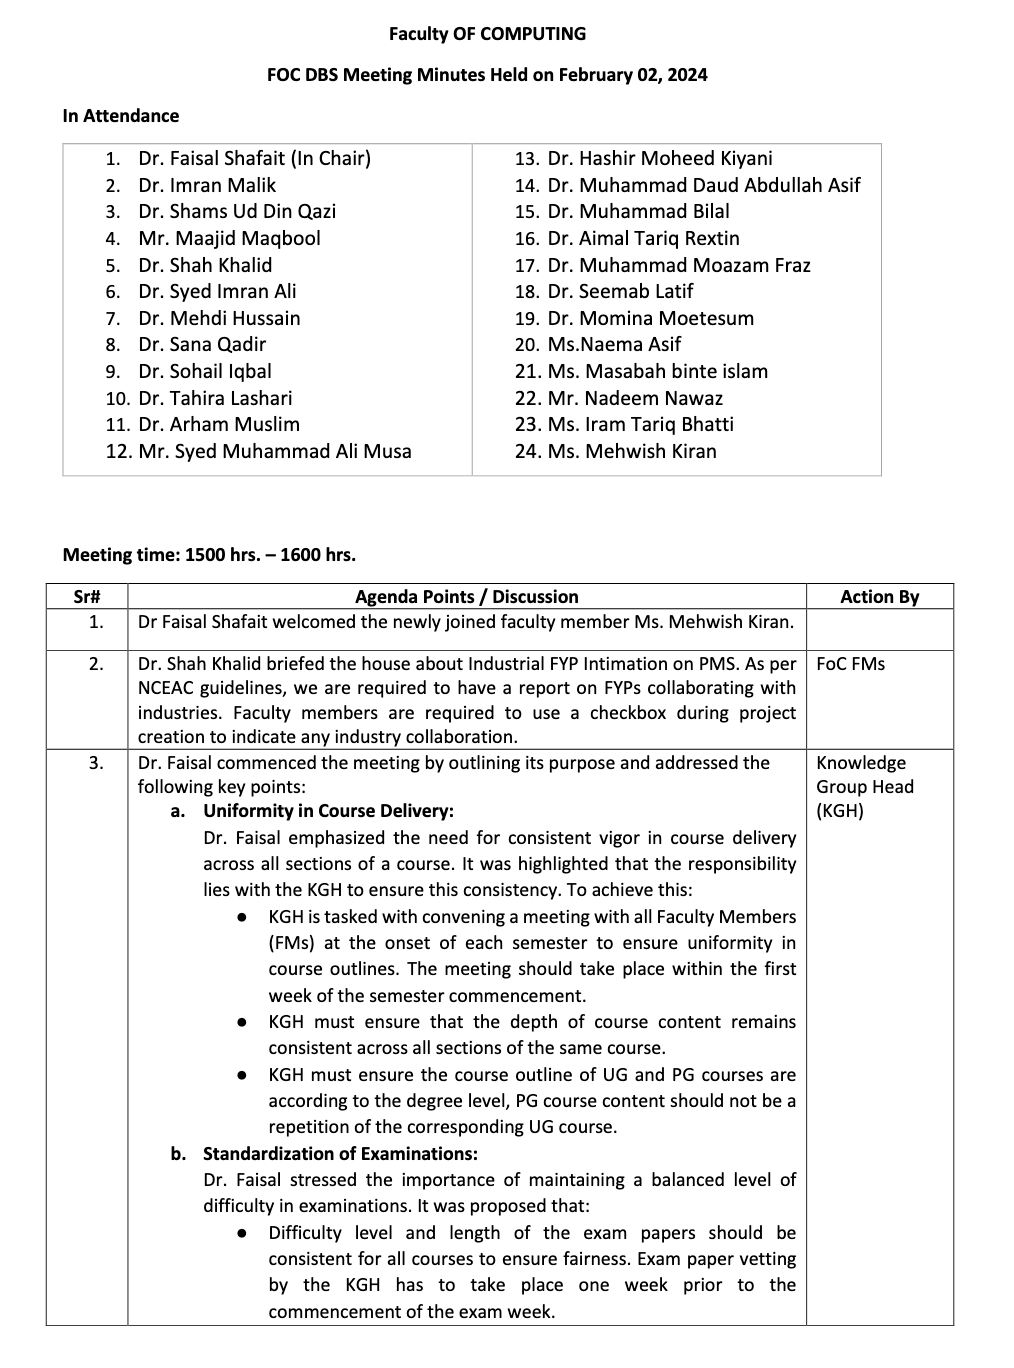
\includegraphics[width=1.0\textwidth]{images/criterion_2/media/dbs-min1.png}
\caption{DBS Meeting Minutes-2nd February 2024}
\end{figure}
\begin{figure}[H]
\centering
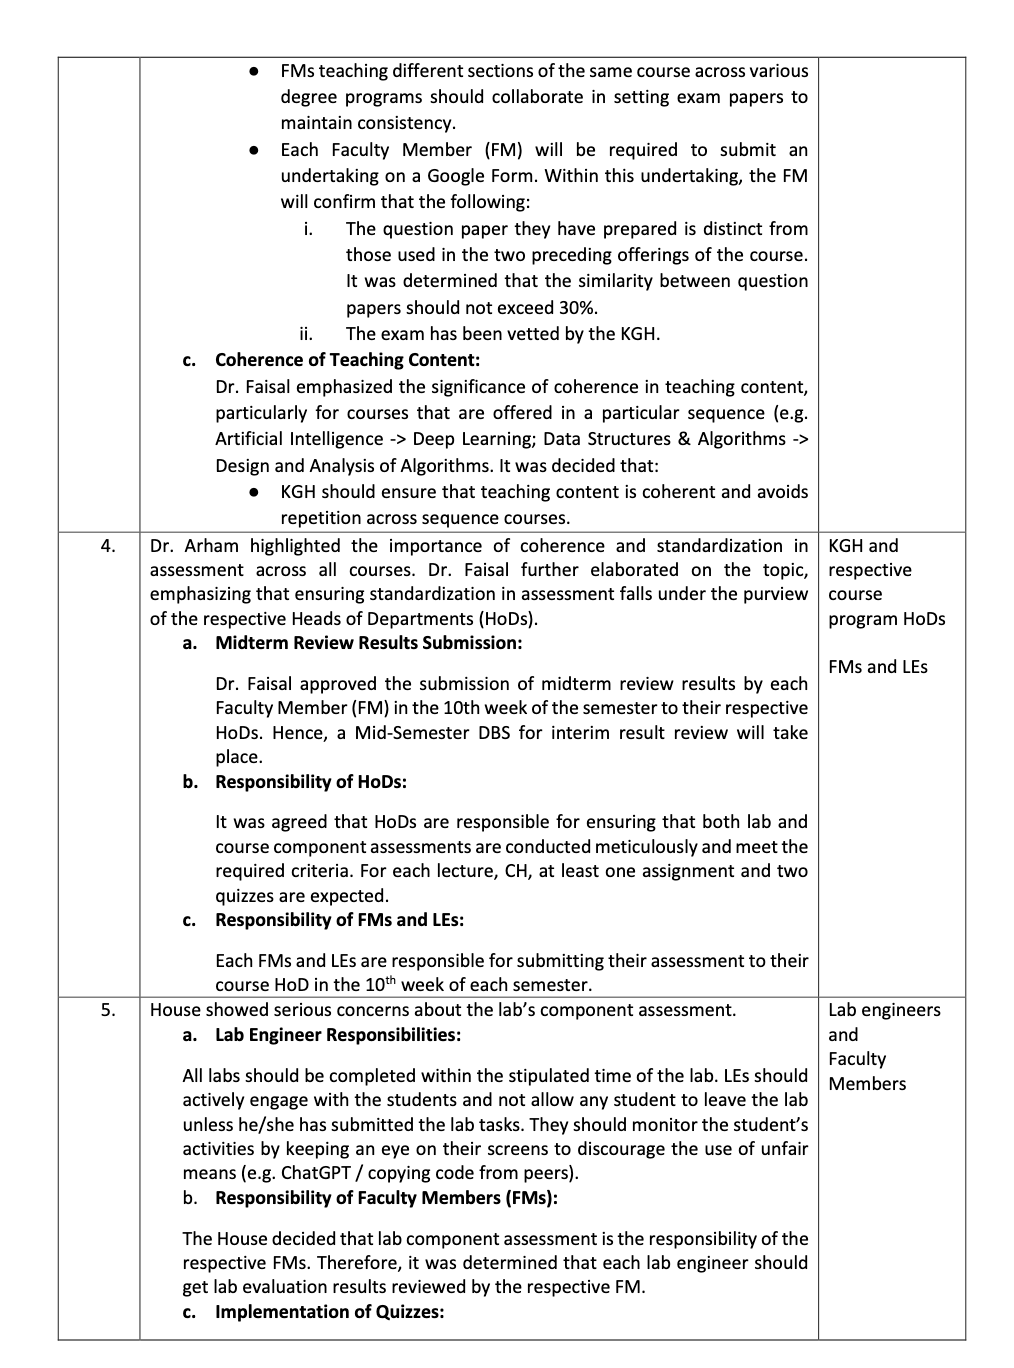
\includegraphics[width=1.0\textwidth]{images/criterion_2/media/dbs-min2.png}
\caption{DBS Meeting Minutes-2nd February 2024}
\end{figure}
\begin{figure}[H]
\centering
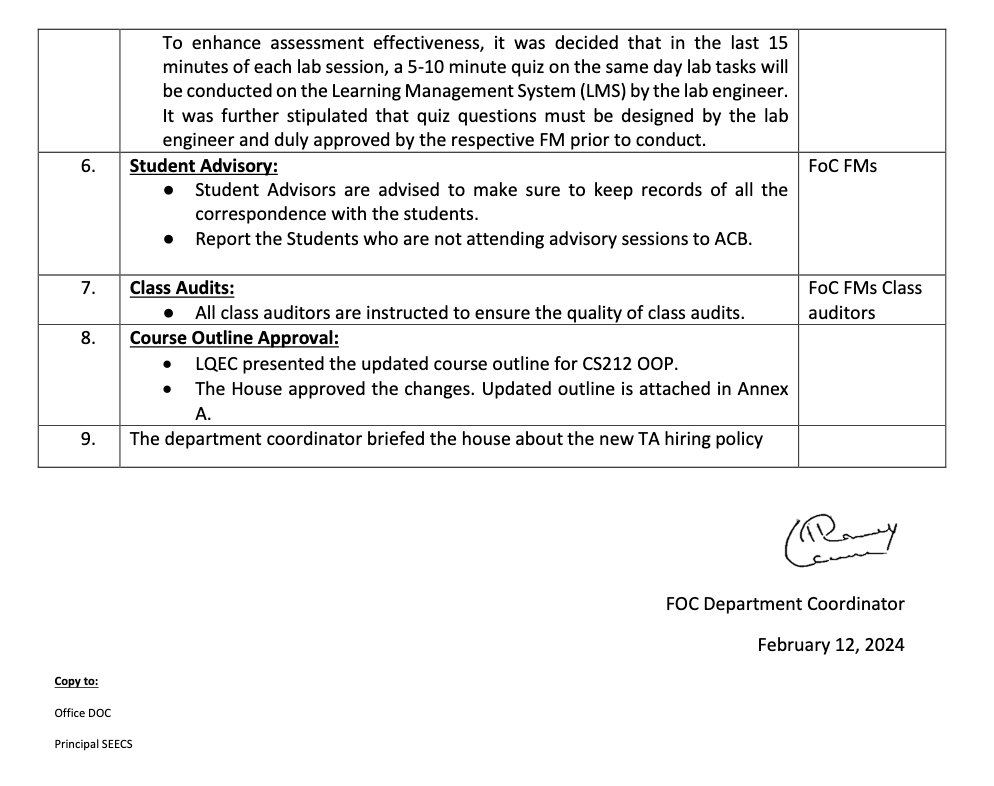
\includegraphics[width=1.0\textwidth]{images/criterion_2/media/dbs-min3.png}
\caption{DBS Meeting Minutes-2nd February 2024}
\end{figure}
\clearpage
\section{Counselling Form}
\label{annex:counselling-form}
\begin{figure}[H]
\centering
\fbox{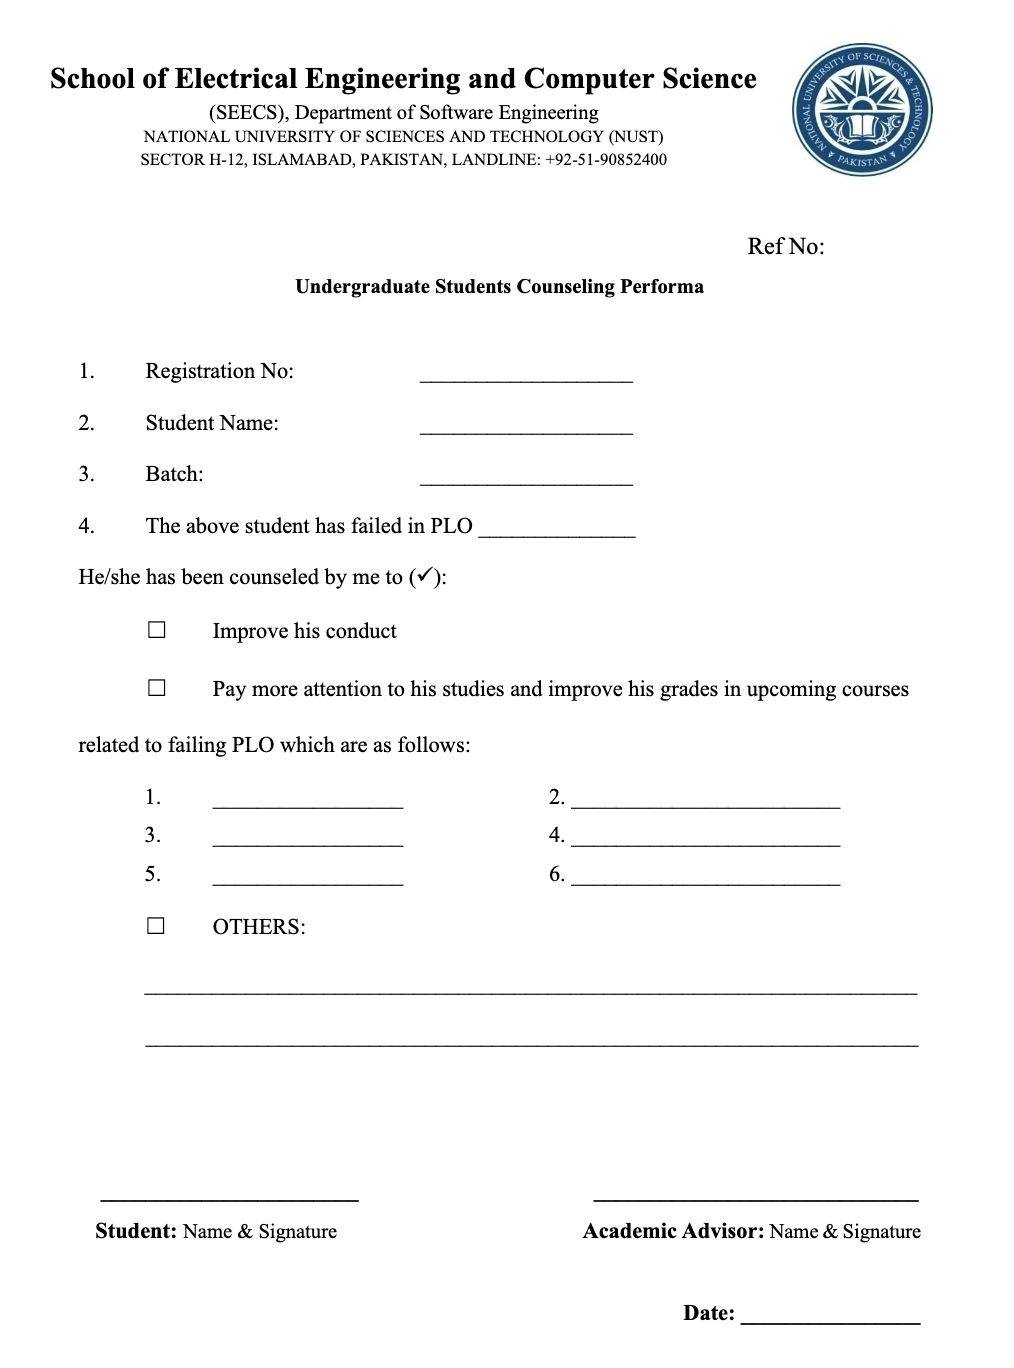
\includegraphics[width=1.0\textwidth]{images/criterion_2/media/council.png}}
\caption{Student Counseling Form}
\end{figure}
%\includefullannexure{appendices/criterion_2/Counselling Form.pdf}

\clearpage
\section{Warning Letter}
\label{annex:warning-letter}
\begin{figure}[H]
\centering
\fbox{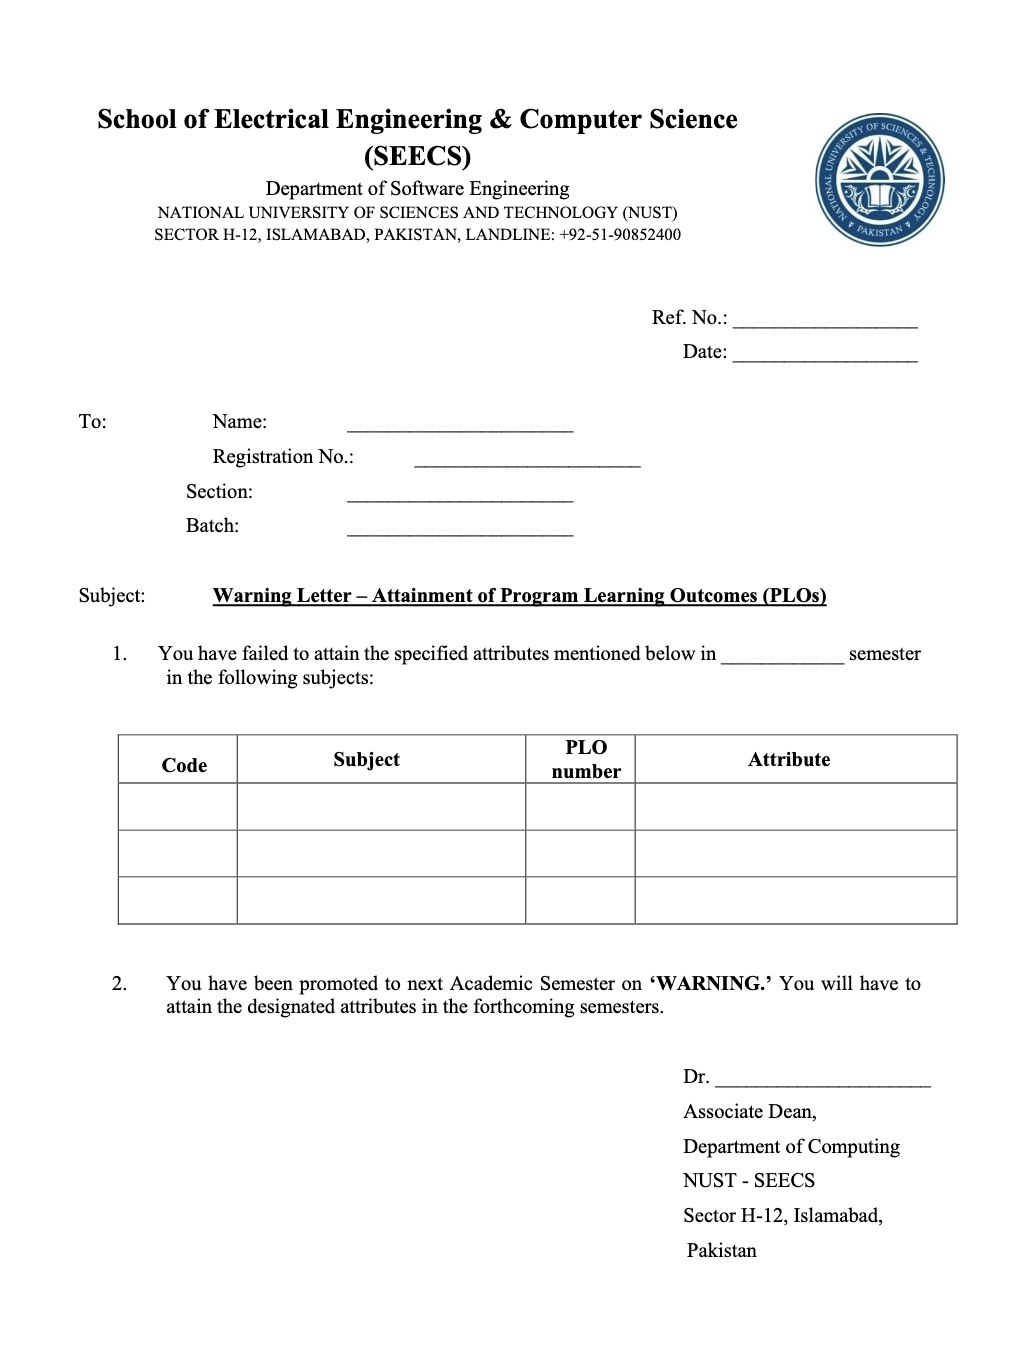
\includegraphics[width=1.0\textwidth]{images/criterion_2/media/warning.png}}
\caption{Sample Warning Letter}
\end{figure}
%\includefullannexure{appendices/criterion_2/Warning Letter.pdf}
\clearpage
\clearpage
\chapter*{Annexure C: Criteria 3 Supporting Documents}
\phantomsection
\addcontentsline{toc}{chapter}{Annexure C: Criteria 3 Supporting Documents}
\label{app:crtieria-3}



% \clearpage
% \phantomsection
% \chapter*{Annexure C: Criteria 3 Supporting Documents}
% \addcontentsline{toc}{chapter}{Annexure C: Criteria 3 Supporting Documents}
% \label{app:crtieria-3}

This section provides supporting annexures required for the Criterion 3: Curriculum and Learning Process.

% \setcounter{section}{0}
% \renewcommand{\thesection}{C.\arabic{section}}

\setcounter{section}{0}
\renewcommand{\thesection}{C.\arabic{section}}
\renewcommand{\theHsection}{annexC.\arabic{section}}


\phantomsection
\section{Intake 2K25 WP No. 30, 72nd ACM}
\label{app:criteria3-intake-2k25-wp30}
The BE Software Engineering (BESE) curriculum at SEECS, NUST, was revised to align the program with the Pakistan Engineering Council (PEC) Engineering Education Guidelines for implementing the Higher Education Commission’s Undergraduate Education Policy (UEP-2024). The revision responds to the mandatory inclusion of specified general education courses in undergraduate engineering programs from Fall 2025 and aims to maintain compliance with the updated credit-hour requirements while preserving the sequence of core Software Engineering courses.

The revised curriculum introduces Fehm-e-Quran-I (1 credit hour) in the first semester and Fehm-e-Quran-II (1 credit hour) in the second semester. Applications of ICT (2+1 credit hours) is also introduced in the first semester. In addition, Pakistan Studies (2 credit hours) is reintroduced as a compulsory course in the fourth semester, replacing the earlier arrangement in which Ideology and Constitution of Pakistan was offered in the first semester. These changes address the prescribed general education requirements under HEC UEP-2024 and the PEC framework.

To maintain an appropriate distribution of credit hours, several existing courses have been relocated between semesters. Occupational Health and Safety and Sociology Elective-II have been moved to the eighth semester, while Expository Writing and Discrete Mathematics have been repositioned within the curriculum. Selected mathematical courses have also been rescheduled. These adjustments help satisfy the minimum requirement of 15 credit hours per semester, where applicable, and the maximum limit of 21 credit hours, without disrupting the progression of core technical courses.

The revision also removes Engineering Drawing and Workshop Practice, which were part of the earlier common first-year engineering structure but are no longer required under the updated PEC curriculum for Software Engineering. Their removal supports compliance with the prescribed maximum of 140 credit hours and creates greater scope for domain-specific and industry-relevant learning. Furthermore, the number of core engineering elective courses has increased from five to six, with corresponding adjustments to elective credit-hour allocations. The semester-wise placement of electives remains flexible, allowing courses to be offered with different credit-hour configurations, as specified in the revised scheme.

Overall, the 2025 revision incorporates the requirements of HEC UEP-2024 and the updated PEC framework while refining course sequencing, elective provision, and credit-hour distribution. The proposal was approved by the Faculty Board of Studies (FBS) on 8 July 2025 and endorsed by the University Curriculum Review Committee (UCRC) on 28 August 2025. The revised unified BE Software program at SEECS and MCS was recommended for implementation from the Fall 2025 batch.
\includefullannexure{appendices/criterion_3/Annex-1-WP-30-72-ACM.pdf}

\clearpage
\phantomsection
\section{Intake 2K24 WP No. 20, 69th ACM}
\label{app:criteria-3_intake-2k24-wp20}

The BE Software Engineering (BESE) curriculum at SEECS, NUST, was revised to align the program with the Pakistan Engineering Council (PEC) Engineering Education Guidelines for the adoption of the Higher Education Commission’s Undergraduate Education Policy (UEP-2023). The revision was proposed in accordance with the PEC framework issued in September 2023 and recommended for implementation in the Fall 2024 intake. The primary objective was to ensure regulatory compliance while maintaining the prescribed credit-hour limits and a balanced distribution of courses across semesters. The revision introduced changes to the humanities component of the curriculum, particularly the knowledge area WK-7: Engineering in Society. In the first semester, the existing English (2 credit hours) course was replaced with Functional English (3 credit hours) to meet the revised requirements. Similarly, Communication Skills (2 credit hours) in the second semester was replaced with Expository Writing (3 credit hours). These changes strengthened the formal English and writing components in accordance with the PEC guidelines. To accommodate the increased credit hours without exceeding the prescribed semester limits, the curriculum was reorganized while retaining a maximum of 18 credit hours per semester where applicable.

The revision also updated the Pakistan-related studies requirement. Pakistan Studies (2 credit hours) in the first semester was replaced with Ideology and Constitution of Pakistan (2 credit hours). In addition, Occupational Health and Safety (1 credit hour) was moved from the first to the second semester, while Islamic Studies (2 credit hours) was shifted from the second to the fourth semester. The revised curriculum provides Ethics (2 credit hours) alongside Islamic Studies in the fourth semester for non-Muslim students, in accordance with the proposed framework. Further adjustments were made to the distribution of humanities and elective courses. Sociology Elective-I was moved from the fourth semester to the fifth semester, where it replaced Technical and Business Writing (2 credit hours), which was removed from the curriculum. These changes reorganized the non-technical course component while preserving the overall structure of the eight-semester degree program.

The revision largely retained the existing technical and core Software Engineering courses, including programming, database systems, data structures and algorithms, software design and architecture, software quality engineering, cloud computing, information security, software project management, and the final-year design project. The changes therefore focused primarily on compliance with the revised PEC requirements and the redistribution of selected humanities and supporting courses rather than a fundamental restructuring of the technical curriculum.

Overall, the revision updated the BESE curriculum to incorporate the requirements associated with HEC UEP-2023 and the PEC framework, strengthened the English and writing components, revised the Pakistan studies requirement, and improved the sequencing of selected courses. The proposal was endorsed by the University Curriculum Review Committee (UCRC) on 23 July 2024 and approved by the Faculty Board of Studies (FBS), as recorded in Working Paper No. 20 for the 69th Academic Council Meeting held on 6 August 2024. The revised curriculum was recommended for implementation in the BE Software Engineering program at SEECS and MCS from the Fall 2024 batch.

\includefullannexure{appendices/criterion_3/Annex-2-WP-20-69-ACM-1-6.pdf}

\clearpage
\phantomsection
\section{Intake 2K19 WP No. 30, 64th ACM}
\label{app:criteria-3_intake-2K19-wp30}
 The program was based on the Pakistan Engineering Council’s 2020 curriculum, which was approved in August 2021. The reason for this revision was a NUST policy change to the Final Year Project (FYP). Previously the FYP carried 3 credit hours in each of the seventh and eighth semesters, but NUST had reduced the seventh-semester load to 2 credit hours and raised the eighth-semester load to 4. This redistribution left some semesters below the minimum regular credit-hour load, so the curriculum needed small adjustments to make up the difference.

The first change is simply the FYP credit split itself: SE-498 (Final Year Project I) now carries 2 credit hours in semester 7, and SE-499 (Final Year Project II) carries 4 credit hours in semester 8. This applies to all ongoing batches, meaning the Fall 2019 intake and everything after it. The remaining changes differ depending on the intake. For the Fall 2019 and Fall 2020 batches, the paper adds a new two-credit Social Science Elective, ECO-130 (Engineering Economics), to the eighth semester. This brings that semester to 12 credit hours and the whole program to 135 credit hours, made up of 110 teaching and 25 lab hours.

For the Fall 2021 and later batches, no new course was added. Instead, two electives swap places. Engineering Elective IV (Data Warehousing and Data Mining), a 3-1 course, moves from semester 7 to semester 8, while MDEE-II (Internet of Things), a 3-0 course, moves from semester 8 to semester 7. This rebalances the workload so both semesters meet the minimum. The program total for these batches is 131 plus X credit hours, where X represents the lab component of certain electives that varies depending on the course chosen. The full revised semester-wise course lists for both groups appear in Annex I and Annex II.

On the practical side, the paper states that no extra instructors or classrooms are required. The proposal was approved by the Faculty Board of Studies on 16 November 2022 and endorsed by the University Curriculum Review Committee on 16 December 2022. The paper itself says the changes take effect from Fall 2022, while the Academics Directorate recommends implementation from Spring 2023 and asks the Academic Council to make the final decision. The stated aim is to keep the BESE program aligned with the PEC’s revised curriculum while improving the quality of final year projects in line with academic and industry needs. Everything else in the existing curriculum remains unchanged.

\includefullannexure{appendices/criterion_3/Annex-3-WP-30-64-ACM.pdf}

\clearpage
\refstepcounter{section}
\phantomsection \label{app:criteria-3_Course Outline with Knowledge Group Head's Signature}
\addcontentsline{toc}{section}{\protect\numberline{\thesection}Course Outline Vetted by Knowledge Group Head}

% ---- Page 1: shrunk, shifted down, heading above it ----
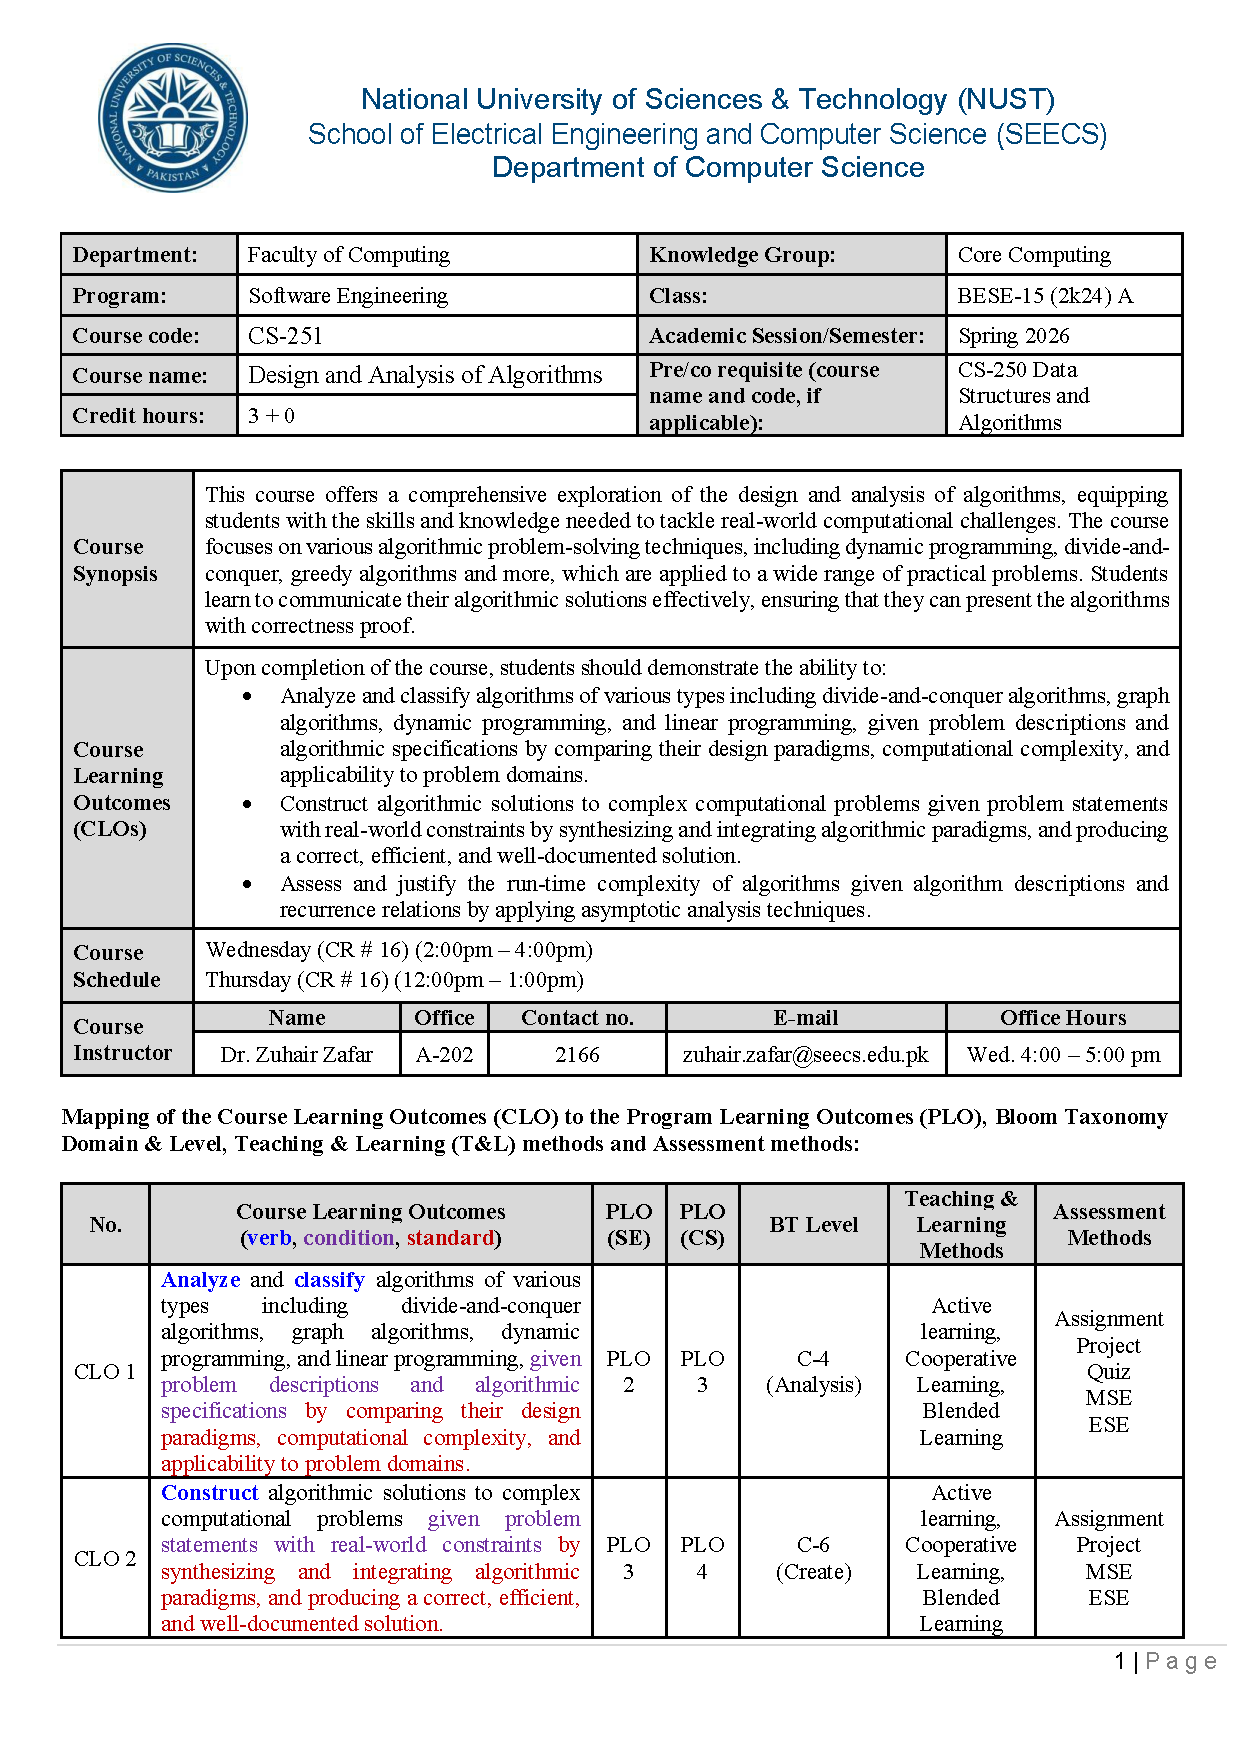
\includepdf[
  pages={1},
  scale=0.85,
  offset=0 -1.5cm,
  pagecommand={\thispagestyle{plain}%
    \noindent{\Large\bfseries\thesection\quad Course Outline Vetted by Knowledge Group Head}}
]{appendices/criterion_3/Annex-4-Course_outline_CS-251 Design and Analysis of Algorithms Spring 2026.pdf}

% ---- Pages 2 to end: unchanged, at full size ----
\includepdf[
  pages={2-},
  pagecommand={\thispagestyle{plain}}
]{appendices/criterion_3/Annex-4-Course_outline_CS-251 Design and Analysis of Algorithms Spring 2026.pdf}

\clearpage
%\section{PLO Attainment Transcript}

\refstepcounter{section}
\phantomsection 
\label{app:criteria-3_PLO Attainment Transcript}
\addcontentsline{toc}{section}{\protect\numberline{\thesection}PLO Attainment Transcript}
\begin{landscape}
% ---- Page 1: shrunk, shifted down, heading above it ----
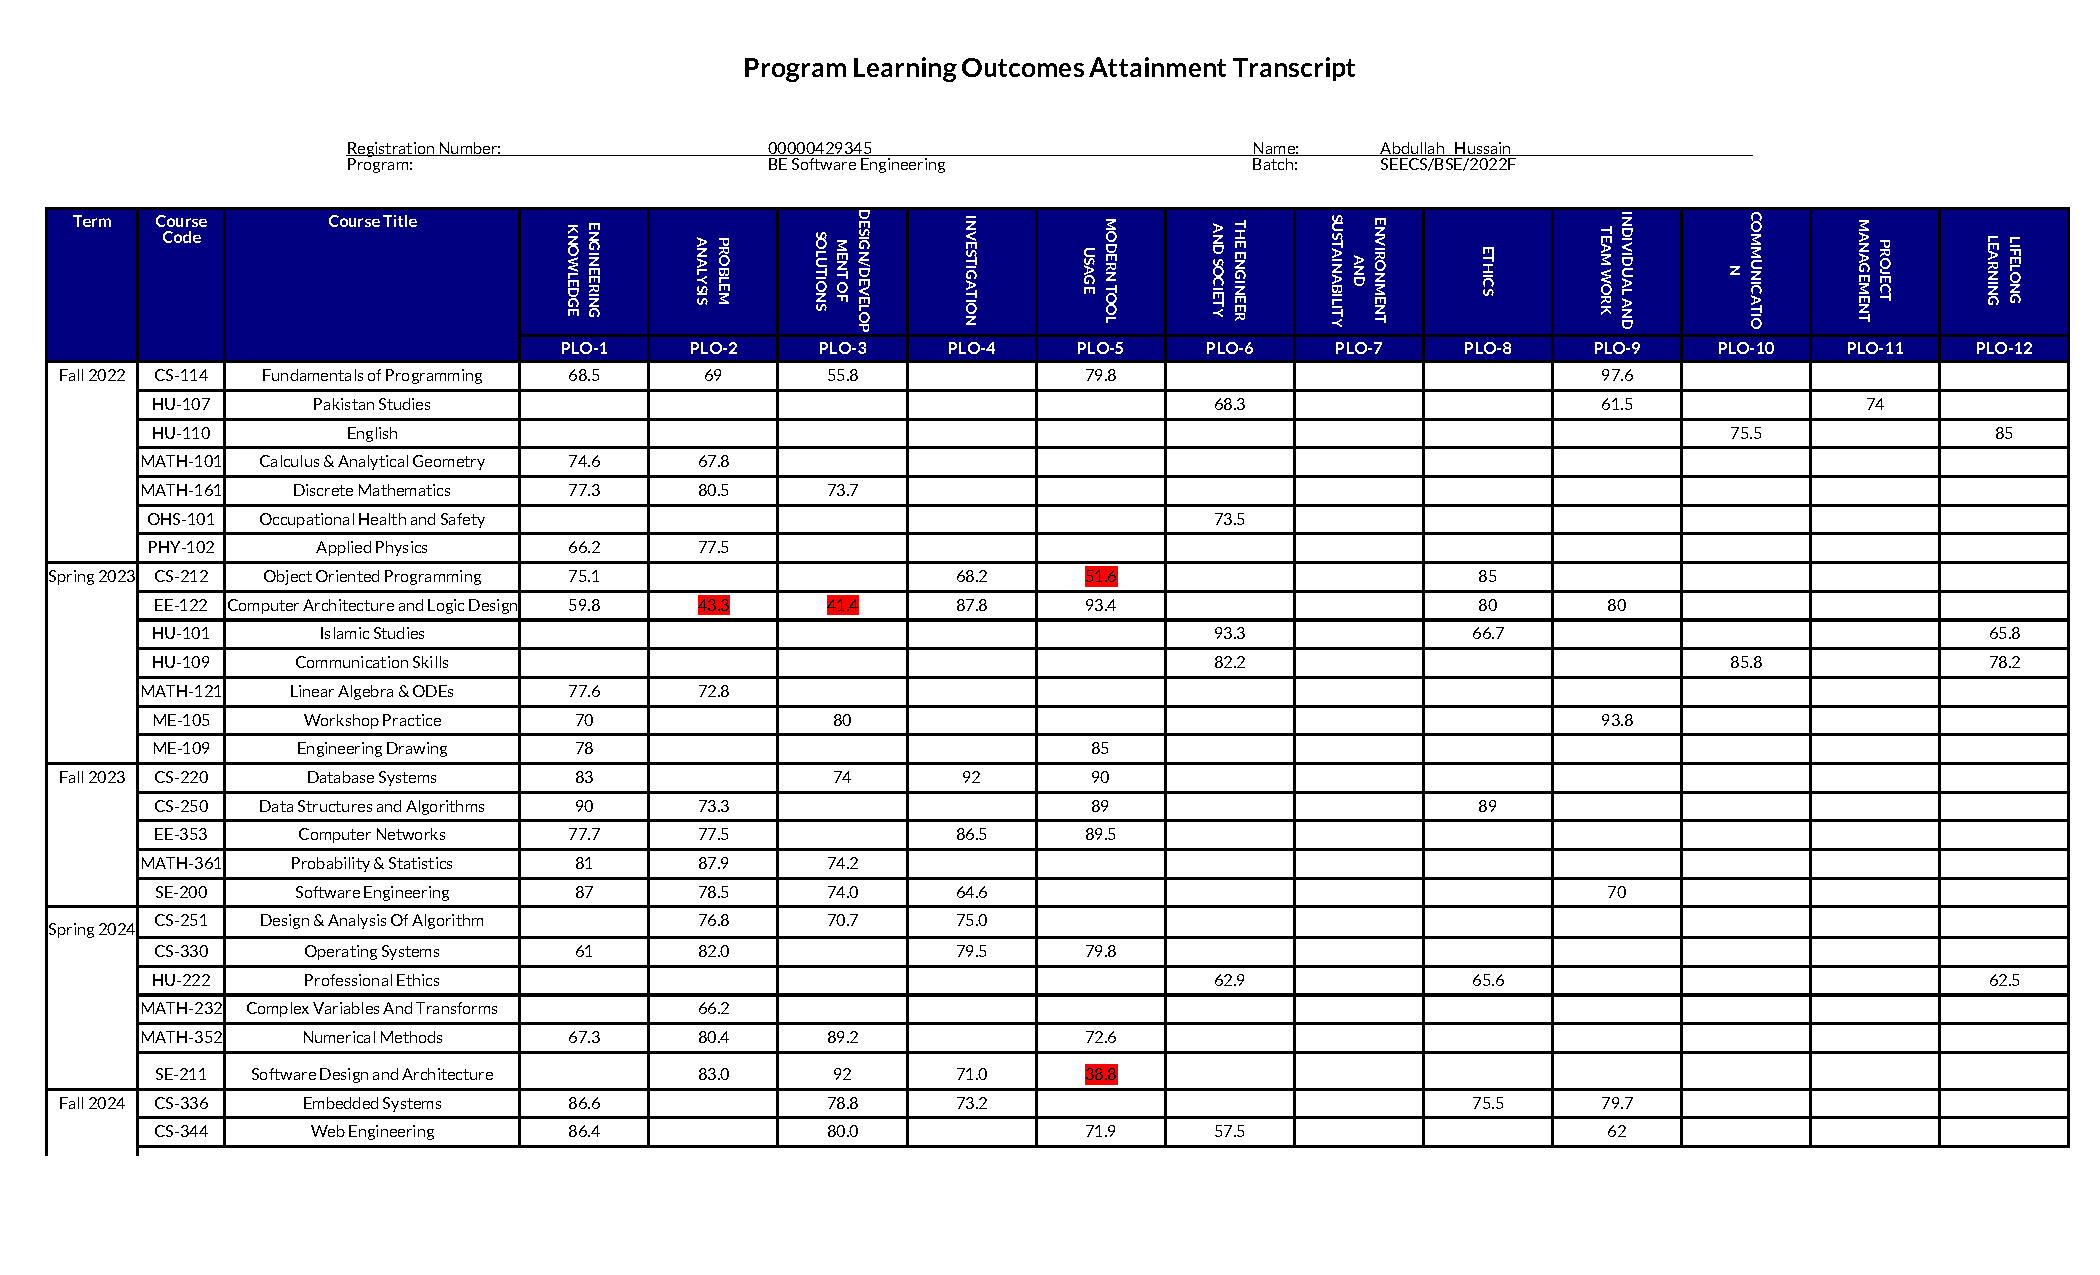
\includepdf[
  pages=1,
    landscape,
    scale=0.80,
  pagecommand={\thispagestyle{plain}%
    \noindent{\Large\bfseries\thesection\quad PLO Attainment Transcript}}
]{appendices/criterion_3/Annex-5-PLO-Attainment-Transcript.pdf}
\end{landscape}
% ---- Pages 2 to end: unchanged, at full size ----
\includepdf[
  pages={2-},
    landscape,
  pagecommand={\thispagestyle{plain}}%
]{appendices/criterion_3/Annex-5-PLO-Attainment-Transcript.pdf}


%\clearpage
%\section{Lab Rubric Based Evaluation}
\clearpage
\refstepcounter{section}
\phantomsection 
\label{app:criteria-3_Lab Rubric Based Evaluation}
\addcontentsline{toc}{section}{\protect\numberline{\thesection}Rubric Based Lab Evaluation}
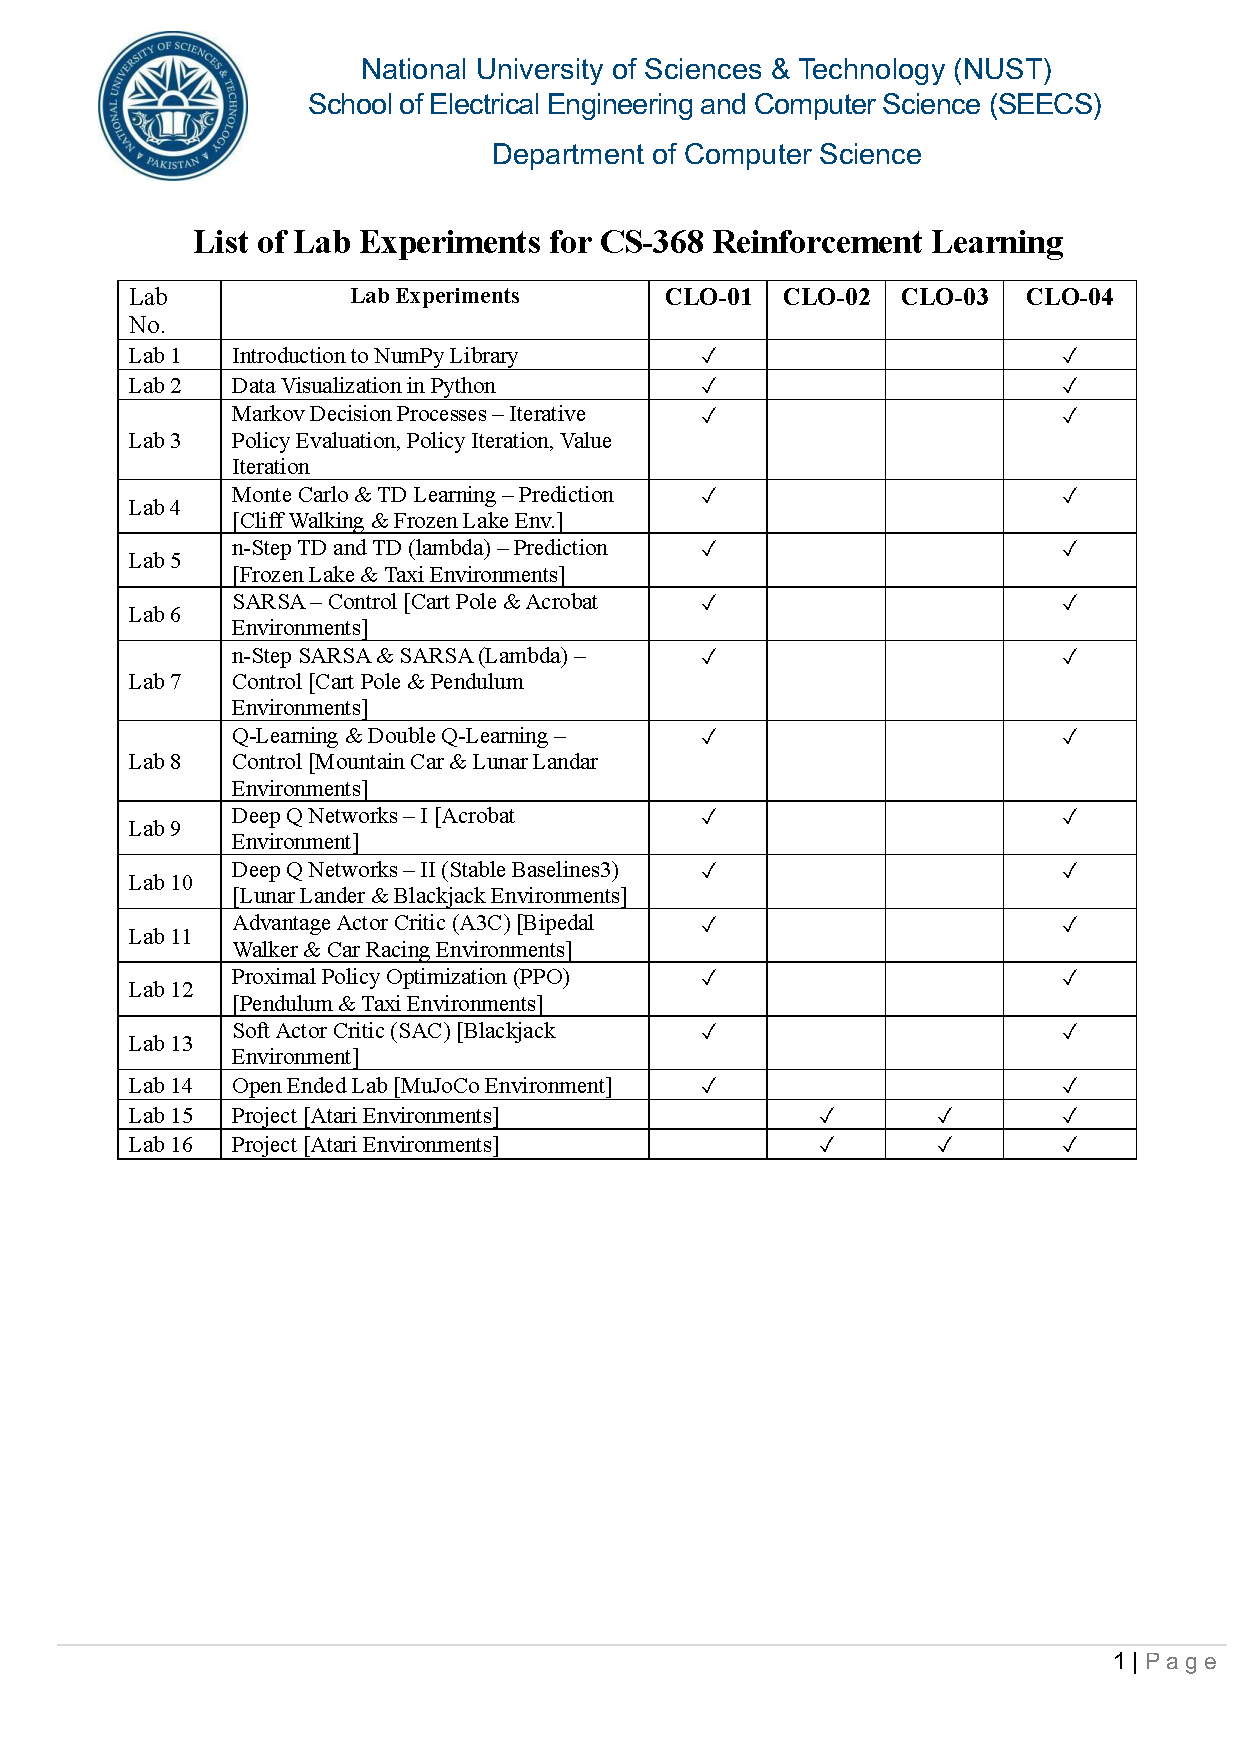
\includepdf[
  pages={1},
  scale=0.85,
  offset=0 -1.5cm,
  pagecommand={\thispagestyle{plain}%
    \noindent{\Large\bfseries\thesection\quad Rubric Based Lab Evaluation}}
]{appendices/criterion_3/Annex-6-Lab-Rubric Based Evaluation.pdf}

\includepdf[
  pages={2-},
  pagecommand={\thispagestyle{plain}}
]{appendices/criterion_3/Annex-6-Lab-Rubric Based Evaluation.pdf}

%\includefullannexure{appendices/criterion_3/Annex-6-Lab-Rubric Based Evaluation.pdf}


%\section{Sample Lab Manual}
\clearpage
\refstepcounter{section}
\phantomsection 
\label{app:criteria-3_Sample Lab Manual}
\addcontentsline{toc}{section}{\protect\numberline{\thesection}Sample Lab Manual}
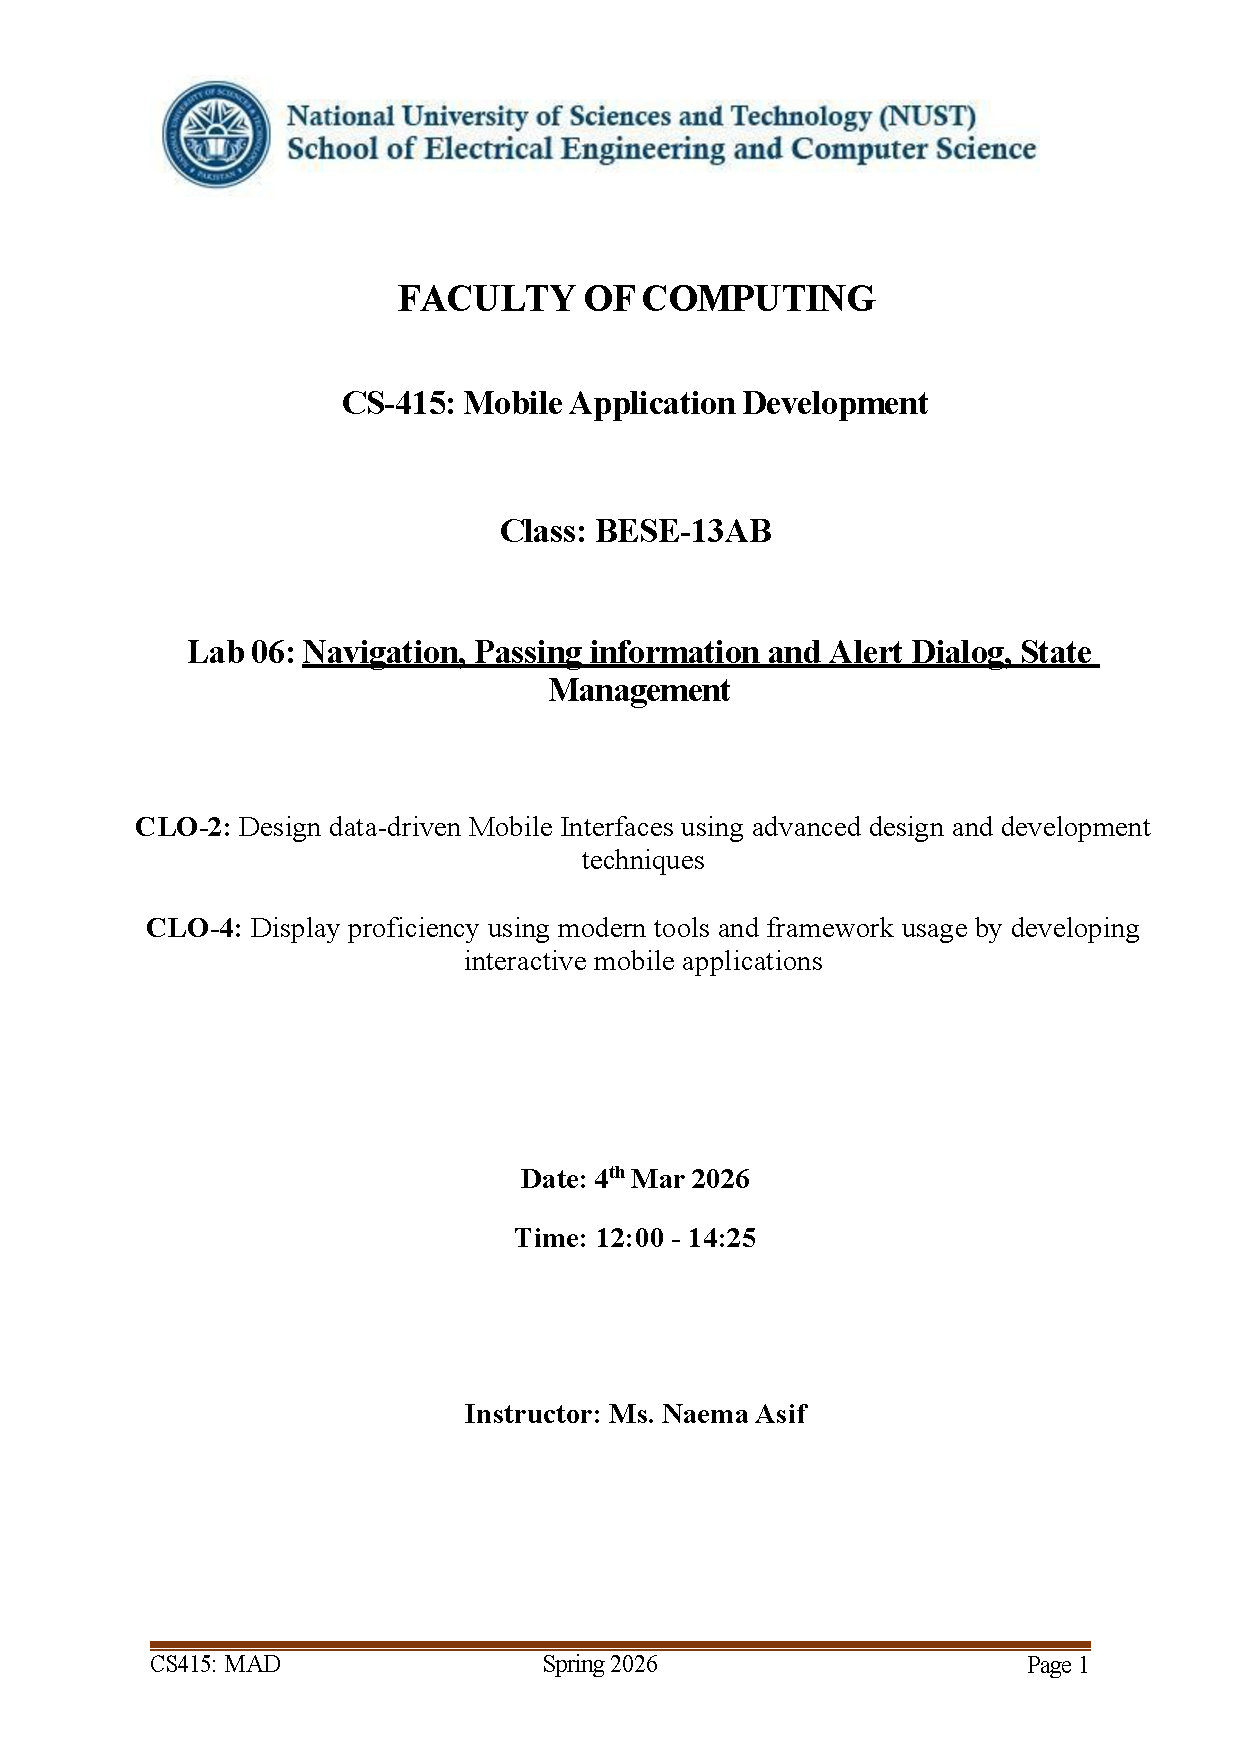
\includepdf[
  pages={1},
  scale=0.85,
  offset=0 -1.5cm,
  pagecommand={\thispagestyle{plain}%
    \noindent{\Large\bfseries\thesection\quad Sample Lab Manual}}
]{appendices/criterion_3/Annex-7-Sample-Lab-Manual.pdf}

\includepdf[
  pages={2-},
  pagecommand={\thispagestyle{plain}}
]{appendices/criterion_3/Annex-7-Sample-Lab-Manual.pdf}
%\includefullannexure{appendices/criterion_3/Annex-7-Sample-Lab-Manual.pdf}

%\clearpage
%\section{Sample Open Ended Lab}
%\label{app:criteria-3_Sample Open Ended Lab}
%\includefullannexure{appendices/criterion_3/Annex-8-Solving-MuJoCo-Environment-Using-RL-(Open-Ended-Lab).pdf}
\clearpage
\refstepcounter{section}
\phantomsection 
\label{app:criteria-3_Sample Open Ended Lab}
\addcontentsline{toc}{section}{\protect\numberline{\thesection}Sample Open Ended Lab}
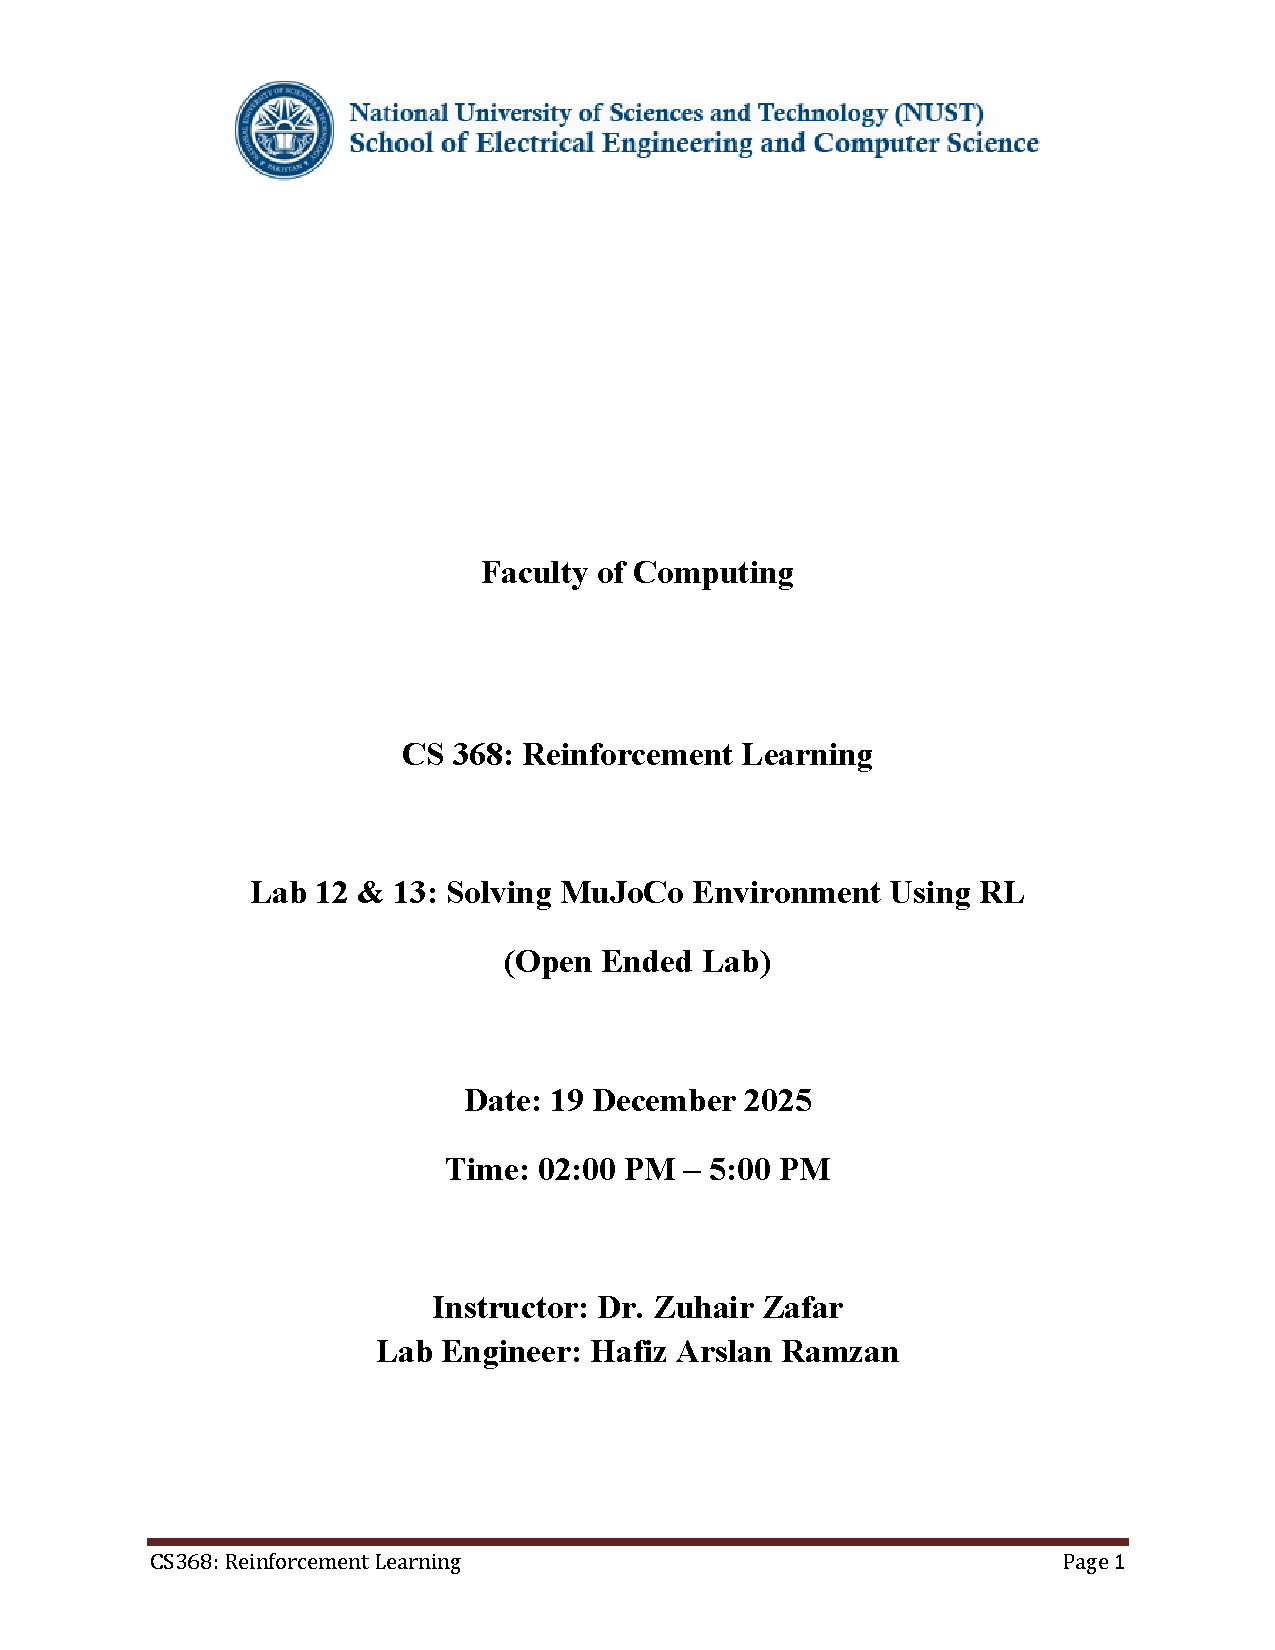
\includepdf[
  pages={1},
  scale=0.85,
  offset=0 -1.5cm,
  pagecommand={\thispagestyle{plain}%
    \noindent{\Large\bfseries\thesection\quad Sample Open Ended Lab}}
]{appendices/criterion_3/Annex-8-Solving-MuJoCo-Environment-Using-RL-(Open-Ended-Lab).pdf}

\includepdf[
  pages={2-},
  pagecommand={\thispagestyle{plain}}
]{appendices/criterion_3/Annex-8-Solving-MuJoCo-Environment-Using-RL-(Open-Ended-Lab).pdf}

\clearpage
%\section{System of Instruction and Examination}
%\includefullannexure{appendices/criterion_3/Annex-9-System-of-instructions-and-examination.pdf}

\refstepcounter{section}
\phantomsection 
\label{app:criteria-3_System of instruction and examination}
\addcontentsline{toc}{section}{\protect\numberline{\thesection}System of Instruction and Examination}
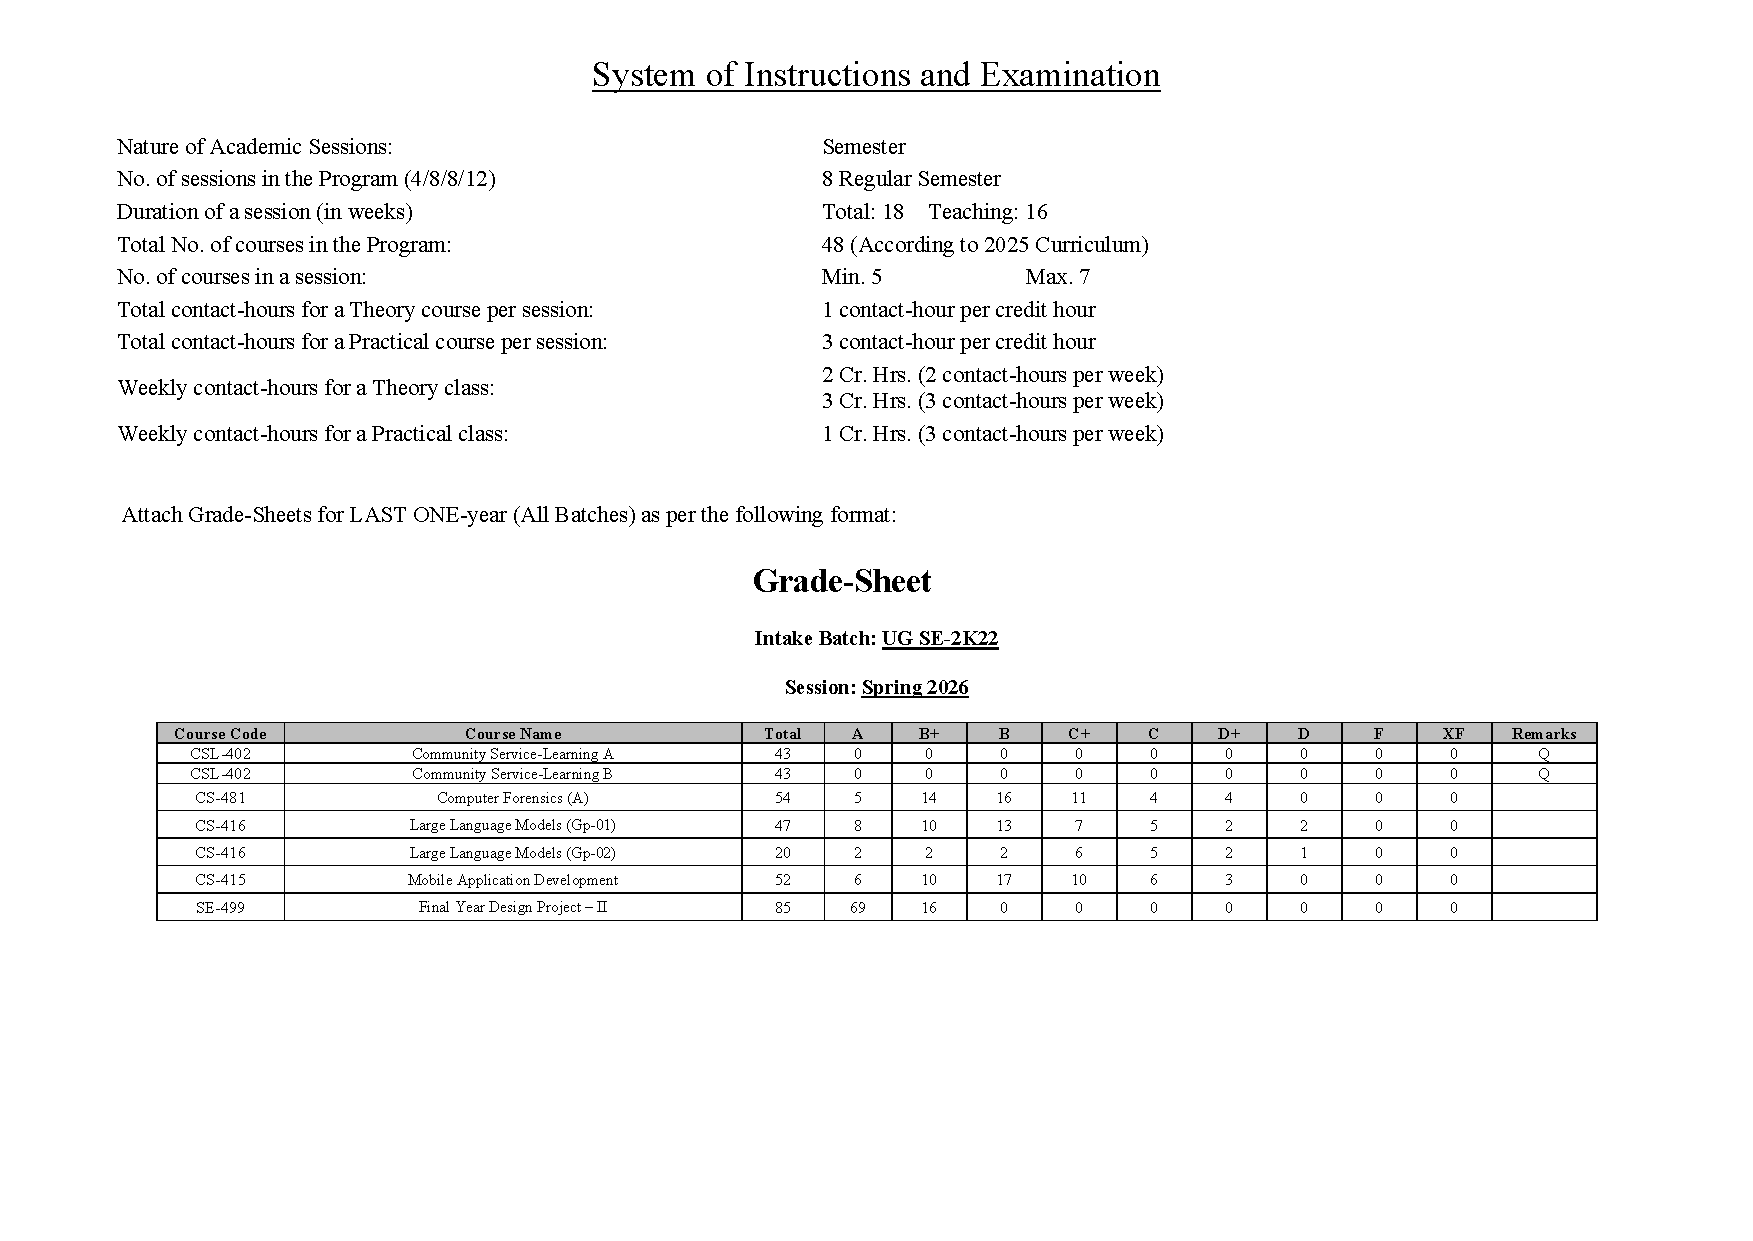
\includepdf[
  pages=1,
  landscape,
  scale=0.85,
  offset=1.5cm 0,
  pagecommand={\thispagestyle{plain}%
    \noindent\rotatebox{90}{\Large\bfseries\thesection\quad System of Instruction and Examination}}
]{appendices/criterion_3/Annex-9-System-of-instructions-and-examination.pdf}
    
\includepdf[
  pages=2-,
  landscape,
  pagecommand={\thispagestyle{plain}}
]{appendices/criterion_3/Annex-9-System-of-instructions-and-examination.pdf}

\clearpage
%\section{CEP Policy for BESE Program}
%\label{app:criteria-3_CEP Policy for BESE Department}
%\includefullannexure{appendices/criterion_3/Annex-10-Request-for-CEP-and-OEL-Formalization.pdf}

%\refstepcounter{section}
%\phantomsection 
%\label{app:criteria-3_CEP Policy for BESE Department}
%\addcontentsline{toc}{section}{\protect\numberline{\thesection}CEP Policy for BESE Program}
%\includepdf[
%  pages={-},
%  scale=0.85,
  %offset=0 -1.5cm,
%  pagecommand={\thispagestyle{plain}%
    %\noindent{\Large\bfseries\thesection\quad CEP Policy for BESE Program}}
%]{appendices/criterion_3/Annex-10-Request-%for-CEP-and-OEL-Formalization.pdf}

%\clearpage
%\section{CEP Policy for BESE Program}
%\label{app:criteria-3_CEP Policy for BESE Department}
%\includefullannexure{appendices/criterion_3/Annex-10-Request-for-CEP-and-OEL-Formalization.pdf}

\clearpage
%\section{CEP Example}
%\label{app:criteria-3_CEP Example}
%\includefullannexure{appendices/criterion_3/Annex-11-Sample-CEP.pdf}

\refstepcounter{section}
\phantomsection 
\label{app:criteria-3_CEP Example}
\addcontentsline{toc}{section}{\protect\numberline{\thesection}CEP Example}
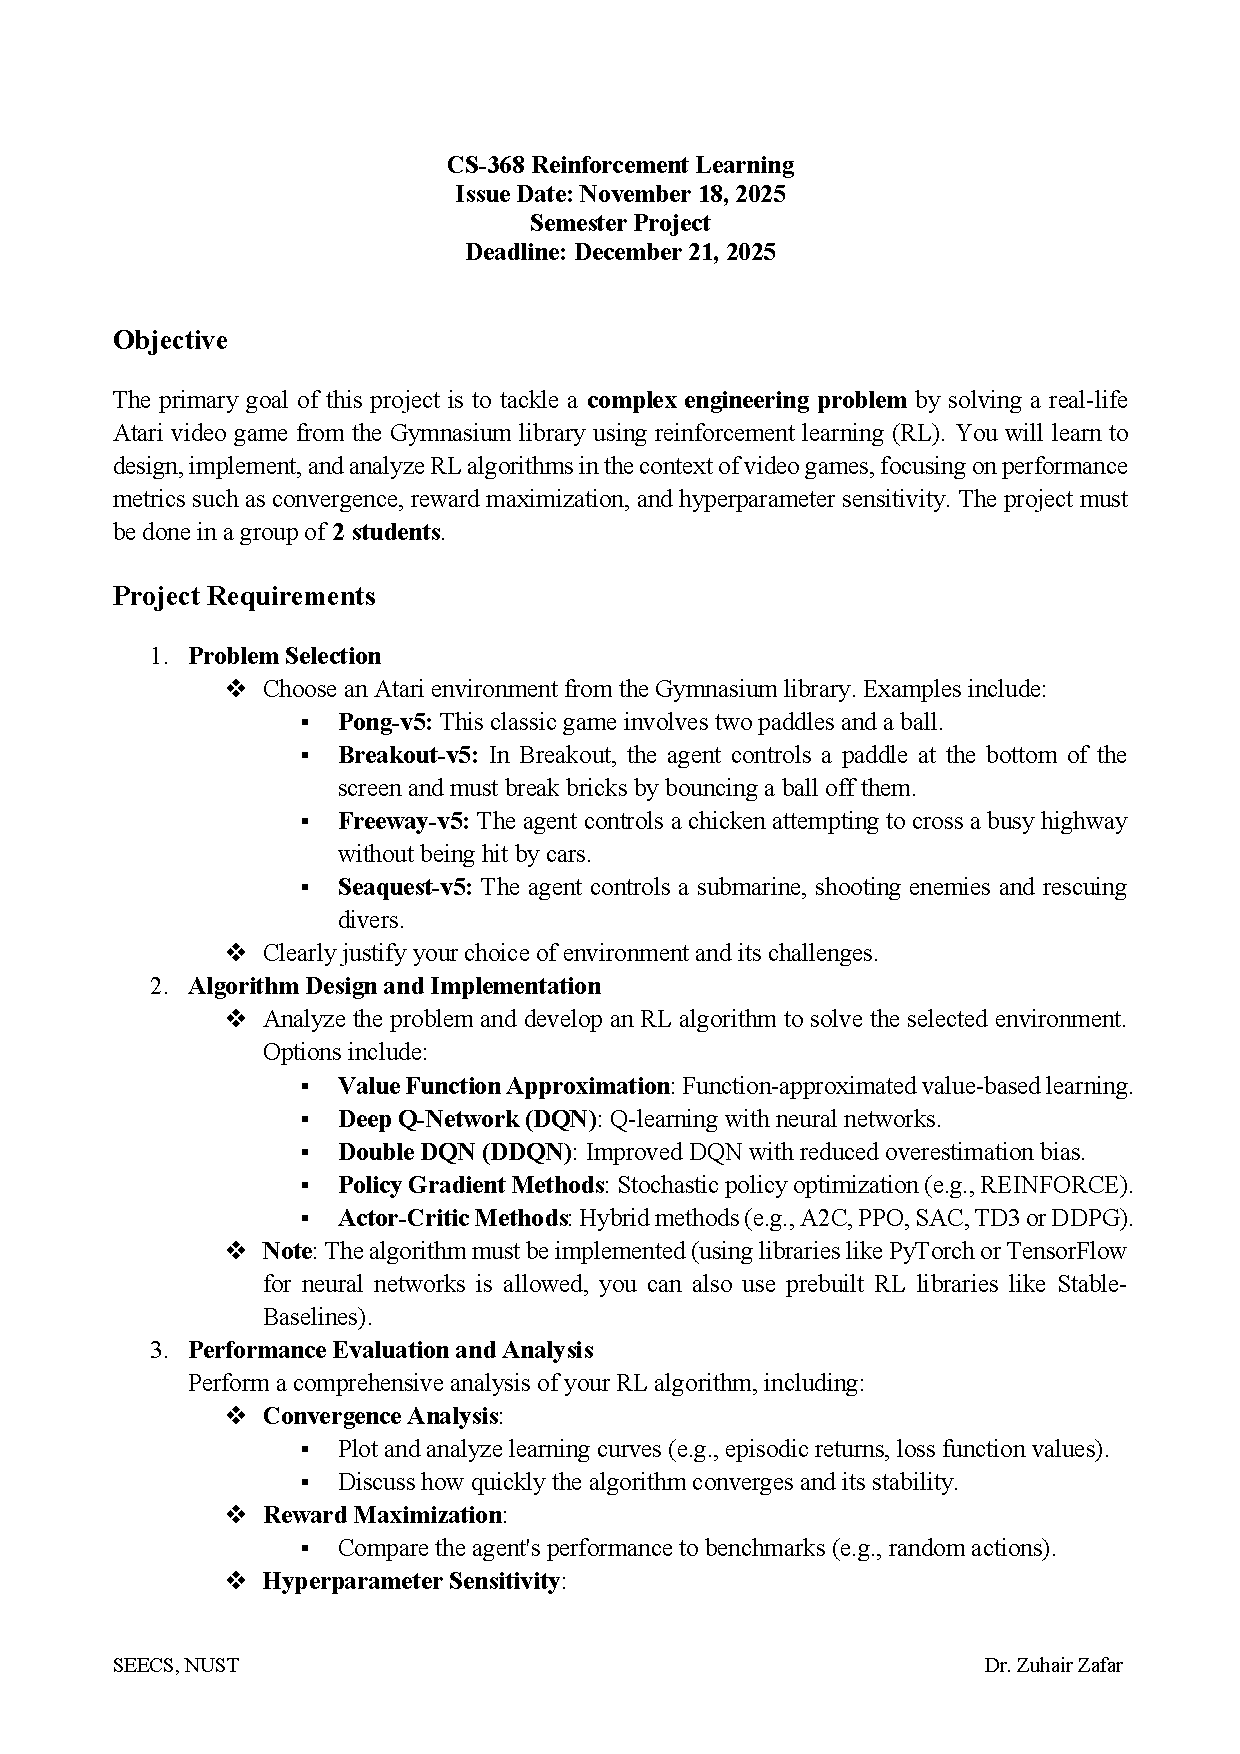
\includepdf[
  pages={1},
  scale=0.85,
  %offset=0 -1.5cm,
  pagecommand={\thispagestyle{plain}%
    \noindent{\Large\bfseries\thesection\quad CEP Example}}
]{appendices/criterion_3/Annex-11-Sample-CEP.pdf}
\includepdf[
  pages=2-,
  %landscape,
  pagecommand={\thispagestyle{plain}}
]{appendices/criterion_3/Annex-11-Sample-CEP.pdf}

\clearpage
\refstepcounter{section}
\phantomsection 
\label{app:criteria-3_FYP_Guidelines}
\addcontentsline{toc}{section}{\protect\numberline{\thesection}FYP Guidelines}

\includepdf[
  pages={1},
  scale=0.85,
  %offset=0 -1.5cm,
  pagecommand={\thispagestyle{plain}%
    \noindent{\Large\bfseries\thesection\quad FYP Guidelines}}
]{appendices/criterion_3/FYDP-SoP-Policy-2026.pdf}

\includepdf[
  pages=2-,
  %landscape,
  pagecommand={\thispagestyle{plain}}
]{appendices/criterion_3/FYDP-SoP-Policy-2026.pdf}

%\section{FYP Guidelines}

%\includefullannexure{appendices/criterion_3/FYDP-SoP-Policy-2026.pdf}

\clearpage
%\section{List of FYDP BESE 2K22 Batch}

%\includefullannexure{appendices/criterion_3/Annex-13-List_FYDP_BESE_2K22.pdf}

\refstepcounter{section}
\phantomsection 
\label{app:criteria-3_List of FYDP BESE 2K22 Batch}
\addcontentsline{toc}{section}{\protect\numberline{\thesection}List of FYDP BESE 2K22 Batch}
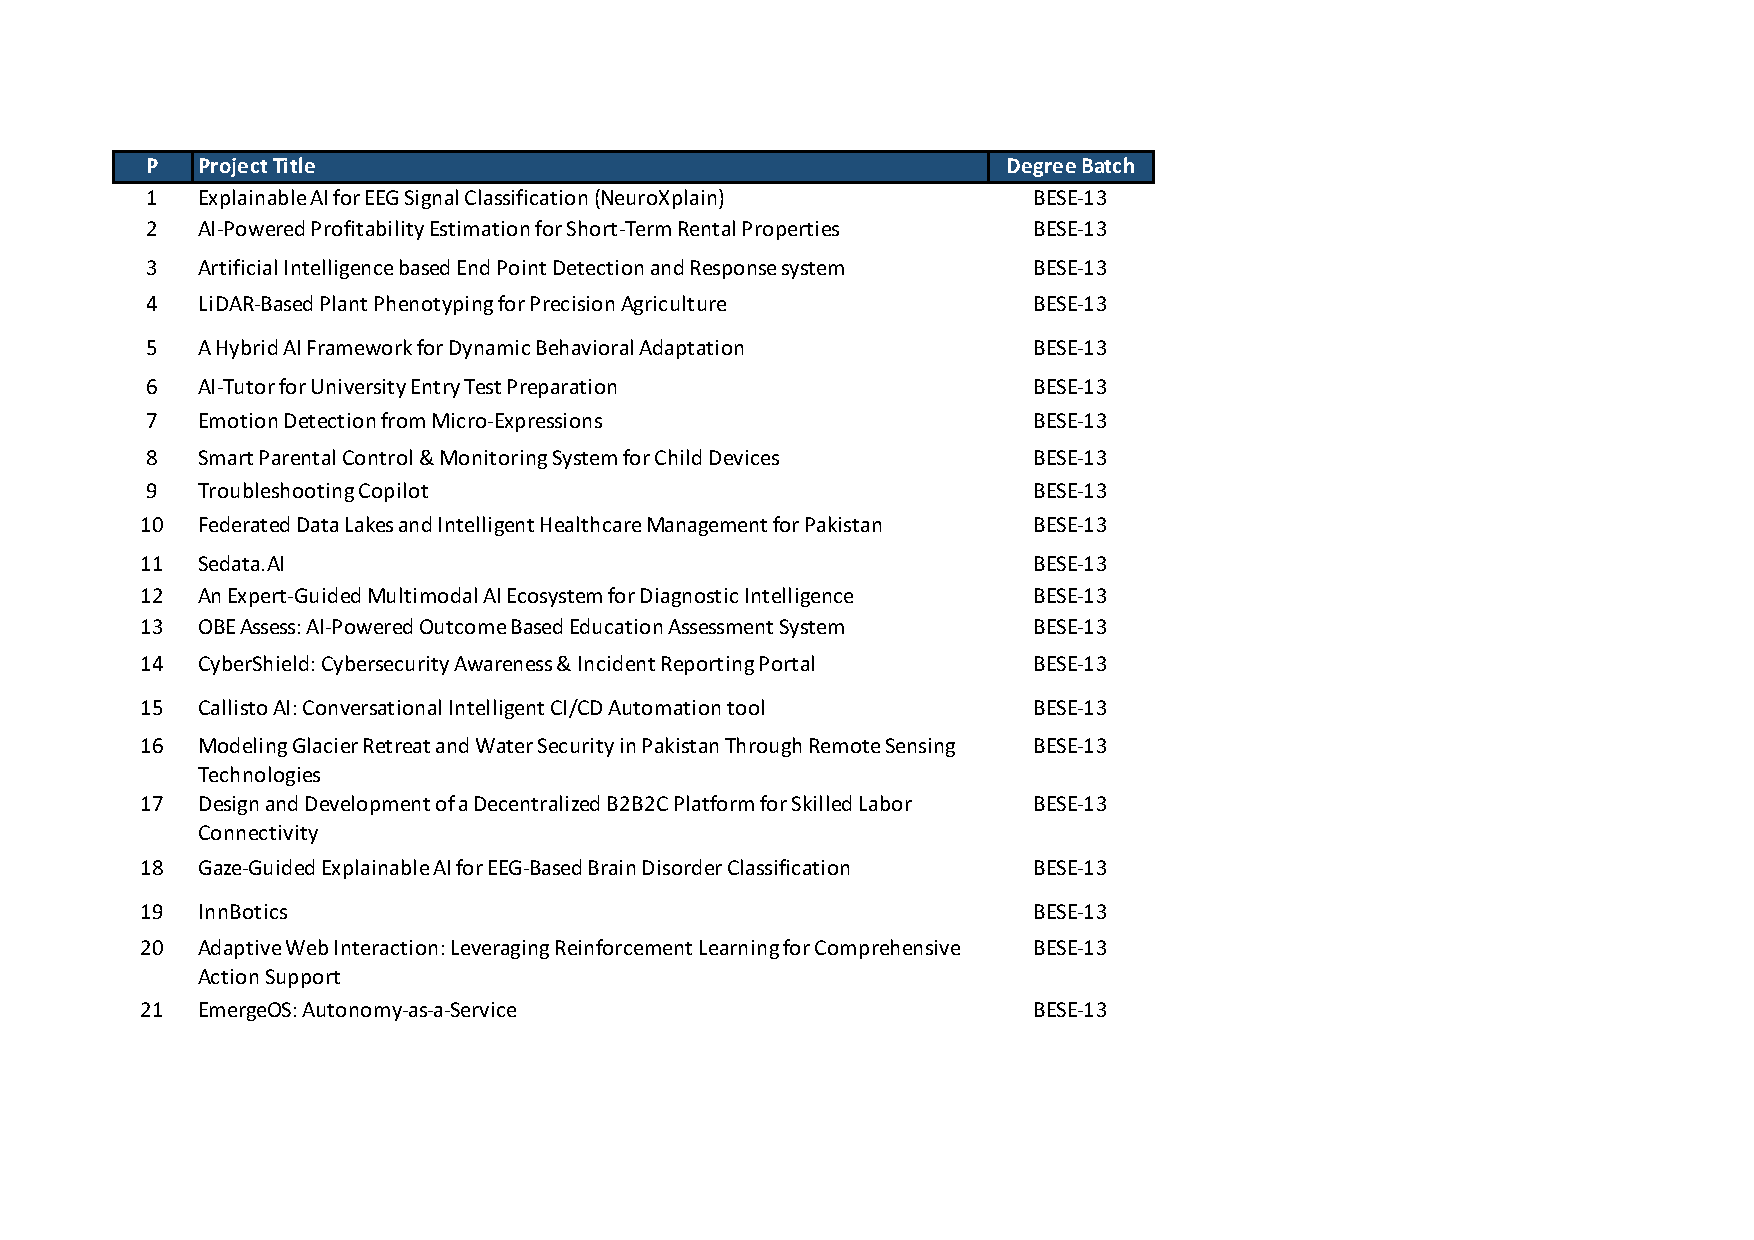
\includepdf[
  pages=1,
  scale=0.85,
  landscape,
  offset=0 -1.5cm,
  pagecommand={\thispagestyle{plain}%
    \noindent{\Large\bfseries\thesection\quad List of FYDP BESE 2K22 Batch}}
]{appendices/criterion_3/fydp-list-2k22.pdf}
    
\includepdf[
  pages=2-,
  landscape,
  pagecommand={\thispagestyle{plain}}
]{appendices/criterion_3/fydp-list-2k22.pdf}

%\clearpage
%\section{Sample Course Outline}
%\label{BSample Course Outline}
%\includefullannexure{appendices/criterion_2/CS-251 Design and Analysis of Algorithms Spring 2026.pdf}


\clearpage
\clearpage
\setcounter{section}{0}
\renewcommand{\thesection}{D.\arabic{section}}
\renewcommand{\theHsection}{annexD.\arabic{section}}

\phantomsection
\addcontentsline{toc}{chapter}{Annexure D: Criteria 4 Supporting Documents}
\label{app:criteria-4}

\refstepcounter{section}
\phantomsection
\label{annex:D1}
\addcontentsline{toc}{section}{\protect\numberline{\thesection}Migration and Transfer Policy}

% ---- Heading block defined as a (long) macro, so \par is allowed ----
\newcommand{\annexDFirstPageHead}{%
  \noindent{\Huge\bfseries Annexure D: Criteria 4 Supporting Documents}\par
  \vspace{0.8em}
  \noindent Here we provide the supporting annexures required for Criterion 4: Students.\par
  \vspace{0.8em}
  \noindent{\Large\bfseries\thesection\quad Migration and Transfer Policy}\par
}

% ---- Page 1: heading + shrunk PDF page ----
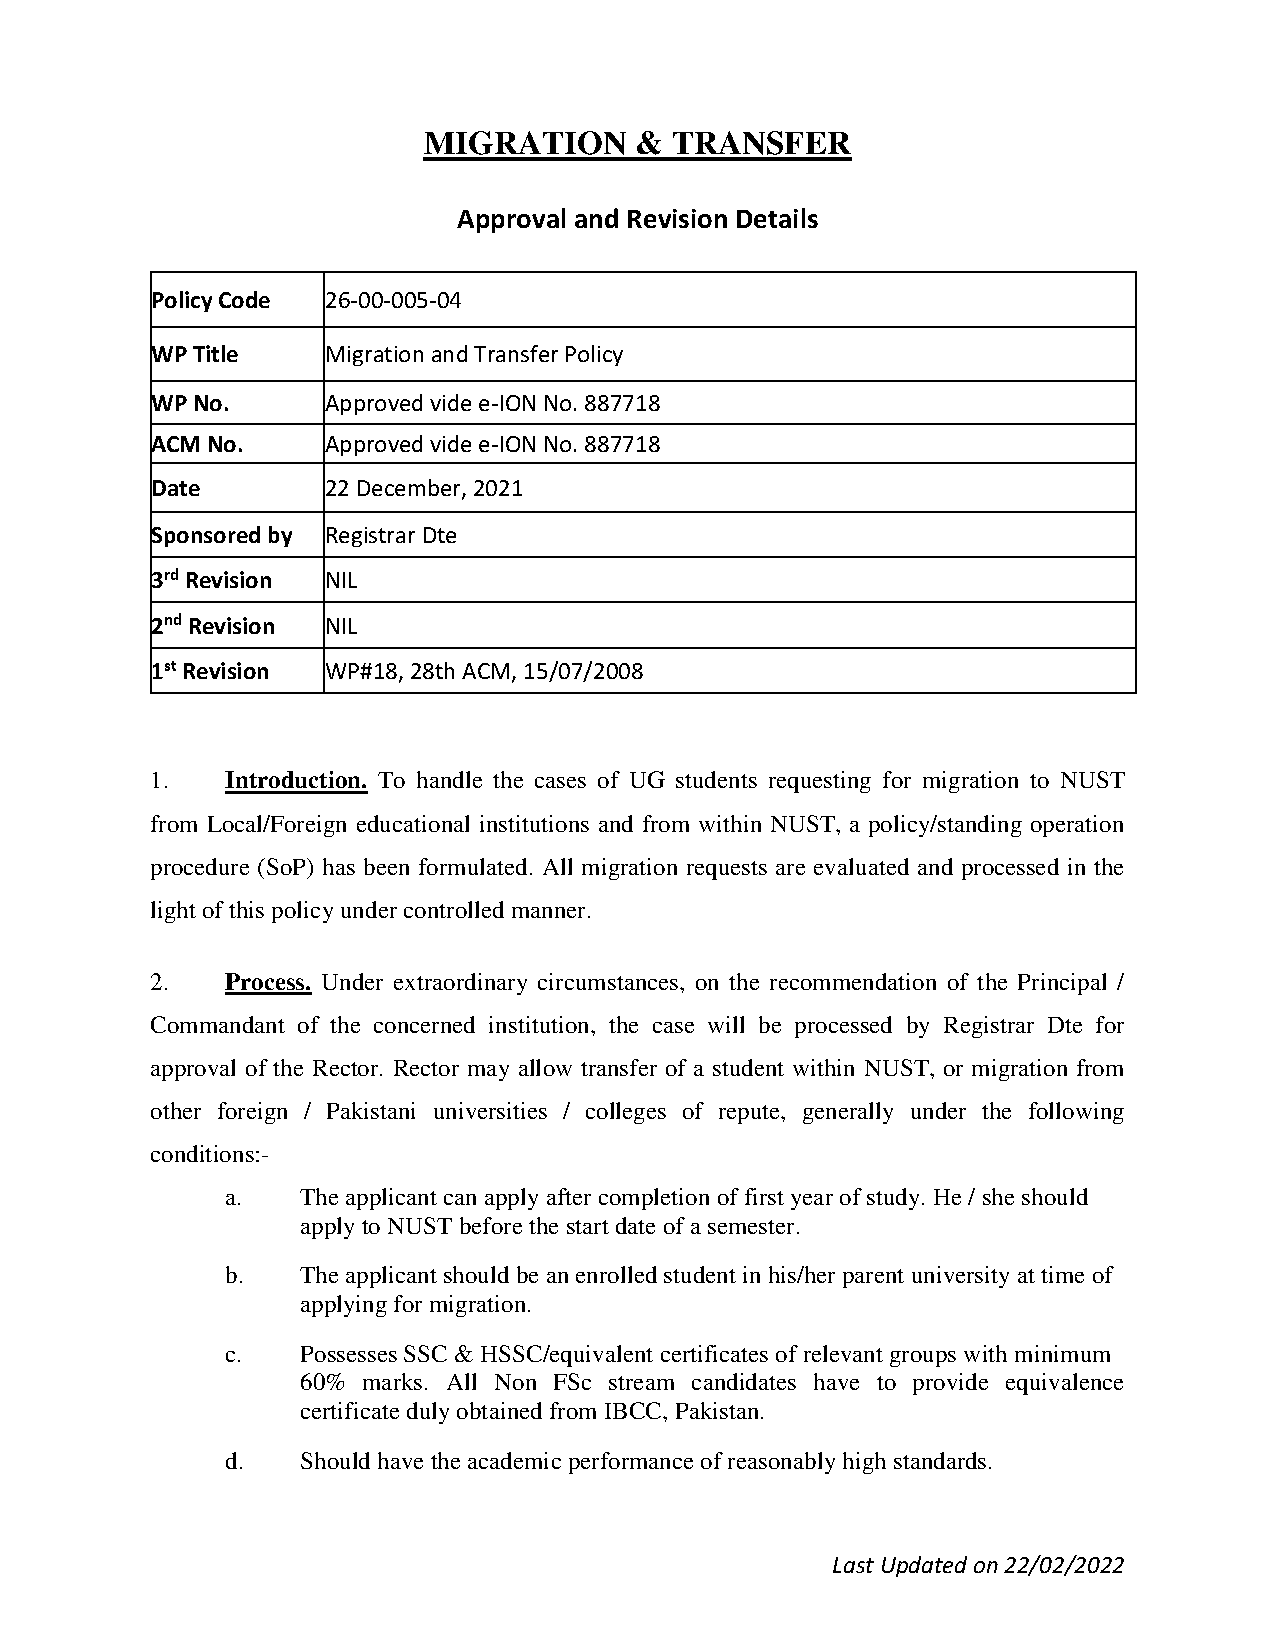
\includepdf[
  pages={1},
  scale=0.68,
  offset=0 -2.2cm,
  pagecommand={\thispagestyle{plain}\annexDFirstPageHead}
]{appendices/criterion_4/Annex D2.pdf}

% ---- Pages 2 to end: unchanged ----
\includepdf[
  pages={2-},
  pagecommand={\thispagestyle{plain}}
]{appendices/criterion_4/Annex D2.pdf}
% ------------------------------------------------------------
\refstepcounter{section}
\phantomsection
\label{annex:D2}
\addcontentsline{toc}{section}{\protect\numberline{\thesection}Migration and Transfer Policy}
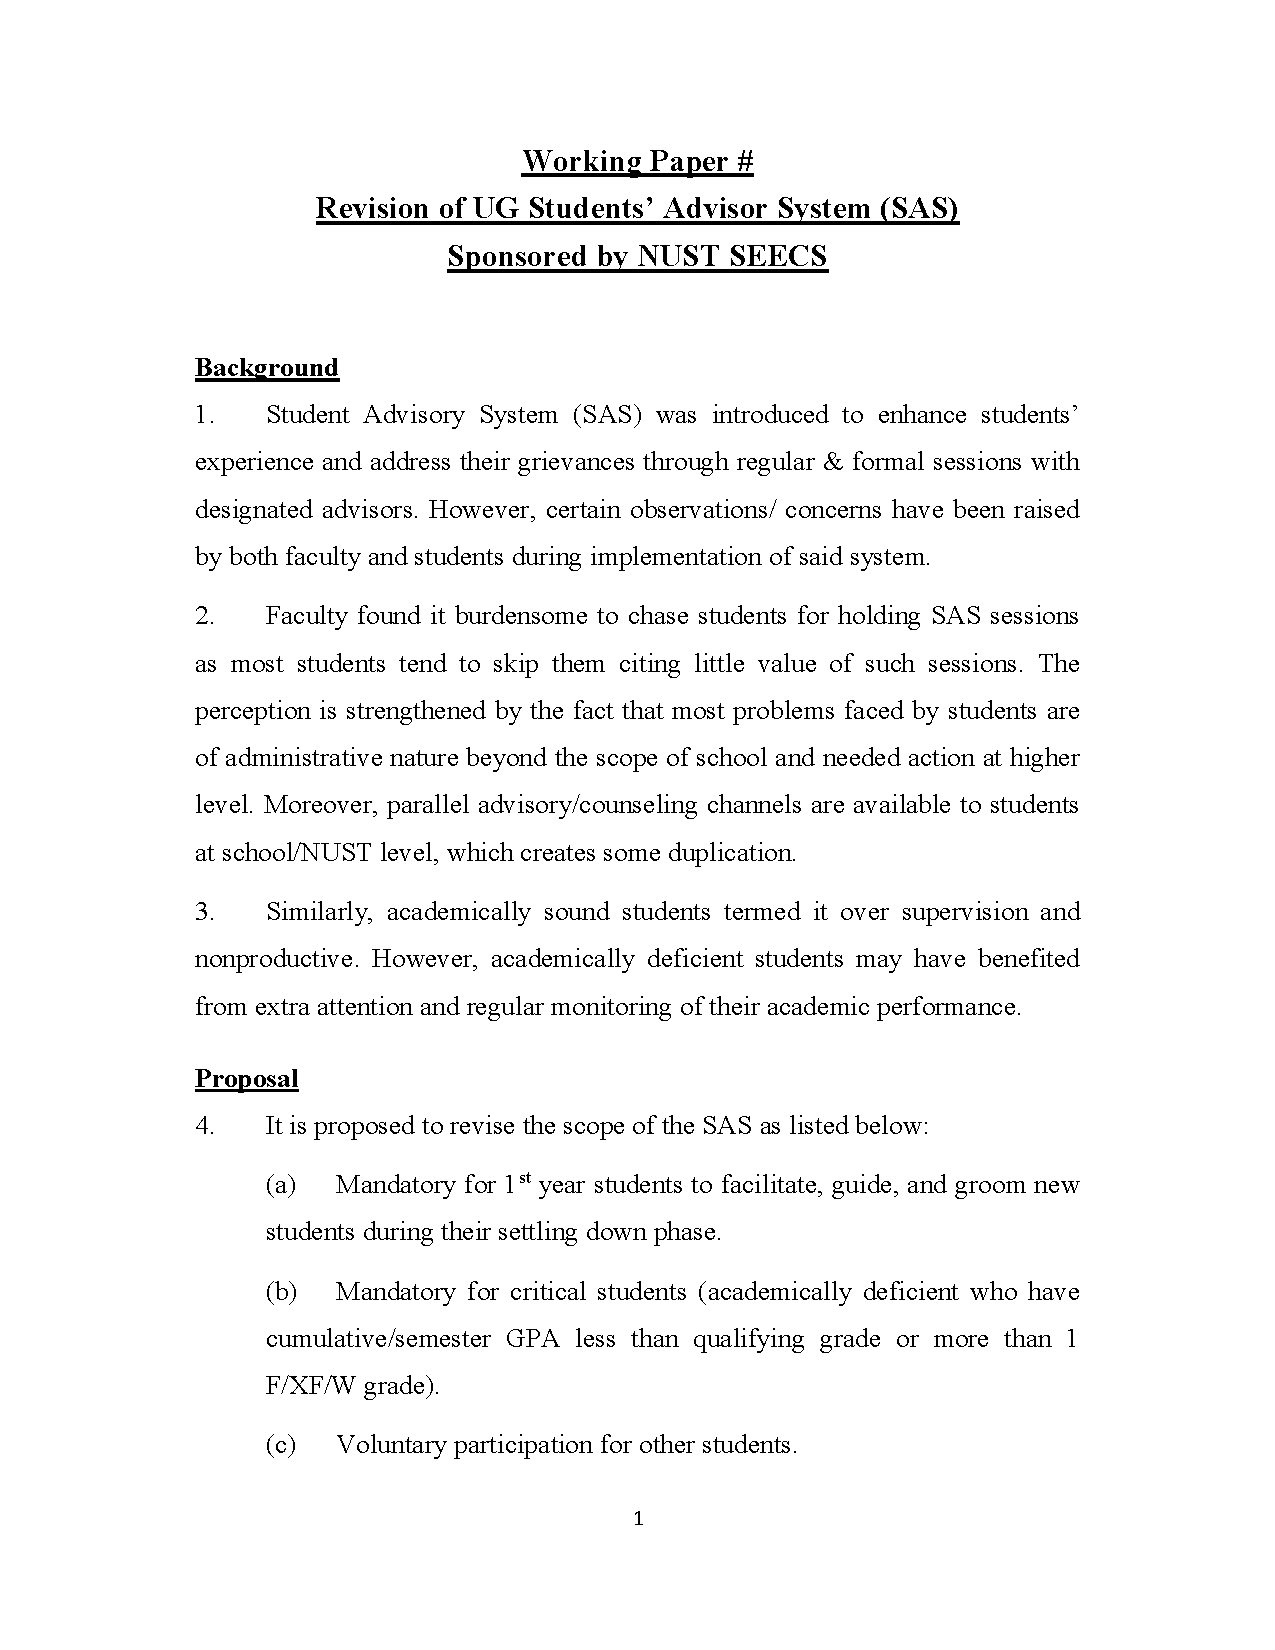
\includepdf[
  pages={1},
  scale=0.85,
  offset=0 -2.2cm,
  pagecommand={\thispagestyle{plain}\noindent{\Large\bfseries\thesection\quad Policy on Student Advisory System}}
]{appendices/criterion_4/Annex D3.pdf}

% ---- Pages 2 to end: unchanged ----
\includepdf[
  pages={2-},
  pagecommand={\thispagestyle{plain}}
]{appendices/criterion_4/Annex D3.pdf}
% ------------------------------------------------------------
\refstepcounter{section}
\phantomsection
\label{annex:D3}
\addcontentsline{toc}{section}{\protect\numberline{\thesection}Student Advisor Feedback Report Template}
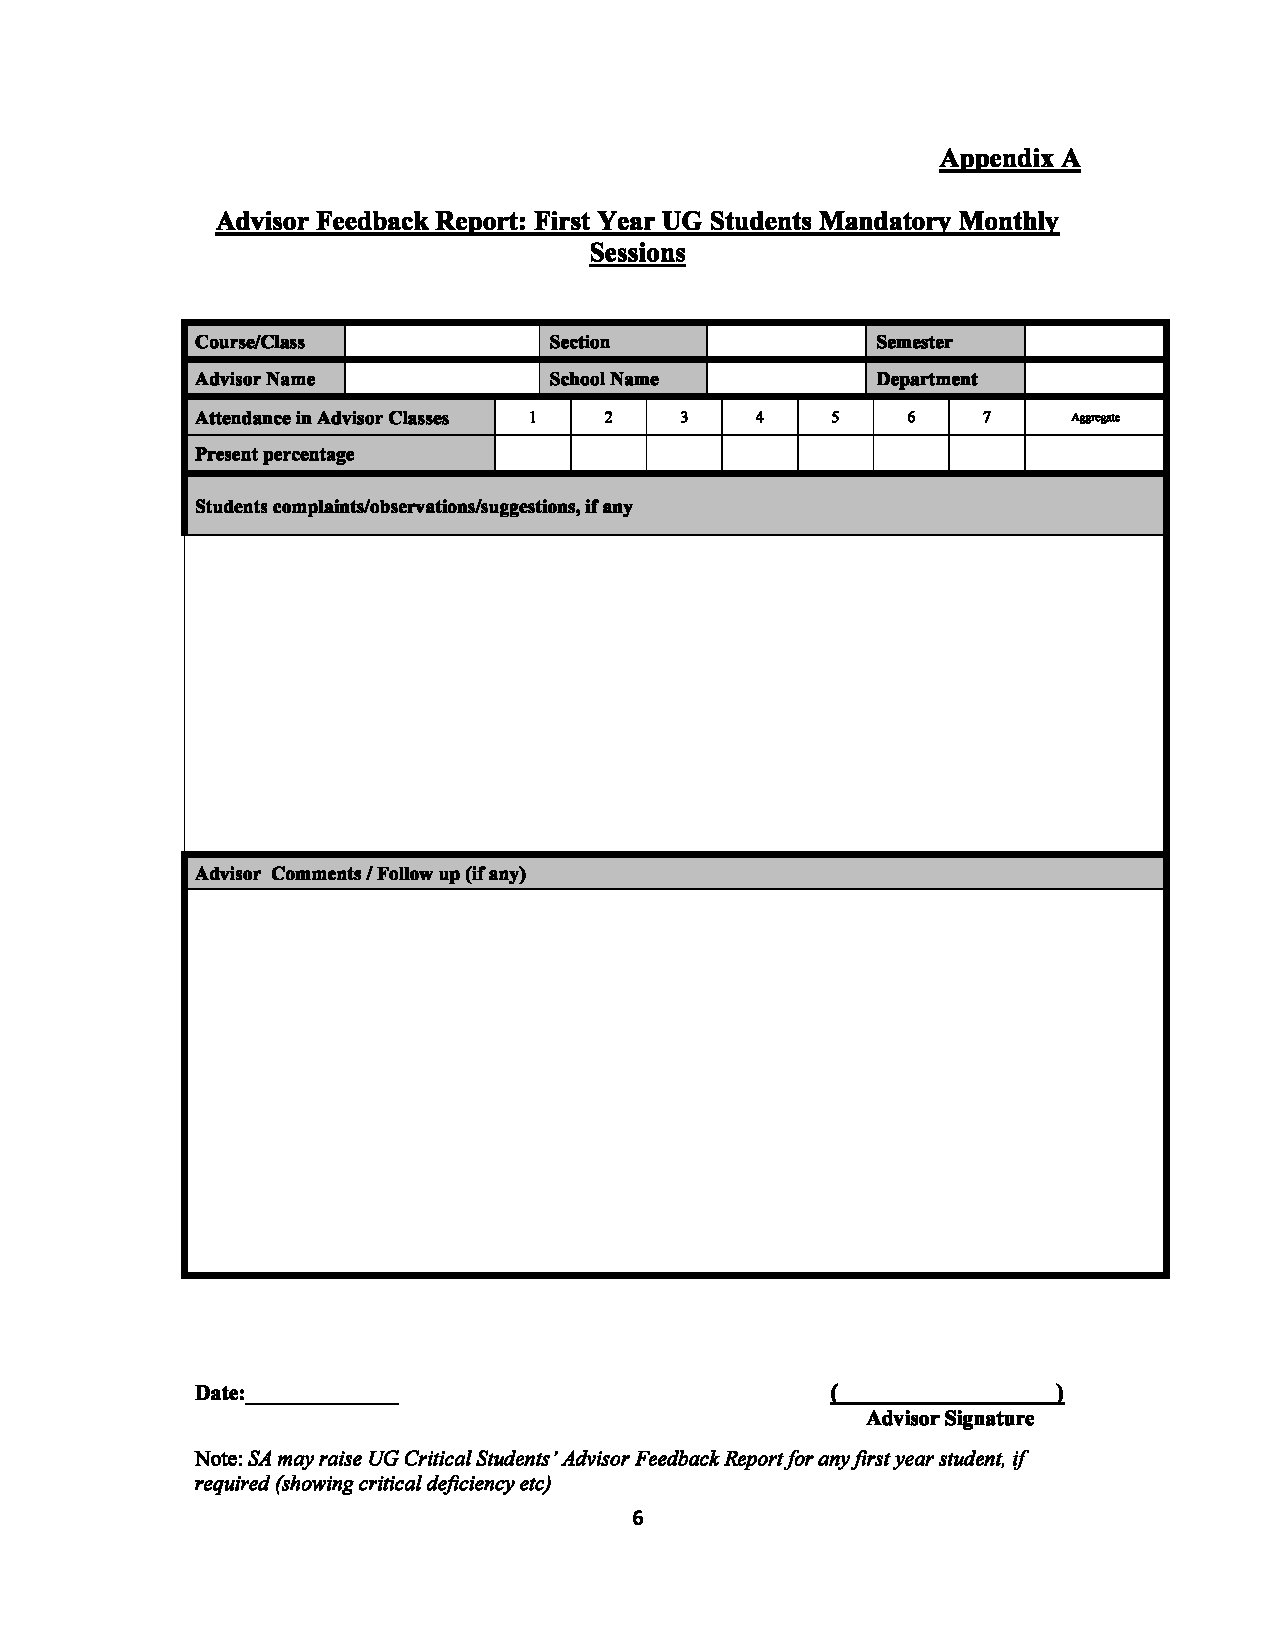
\includepdf[
  pages={1},
  scale=0.85,
  offset=0 -2.2cm,
  pagecommand={\thispagestyle{plain}\noindent{\Large\bfseries\thesection\quad Student Advisor Feedback Report Template}}
]{appendices/criterion_4/Annex D4.pdf}
\includepdf[
  pages={2-},
  pagecommand={\thispagestyle{plain}}
]{appendices/criterion_4/Annex D4.pdf}

% ------------------------------------------------------------
\refstepcounter{section}
\phantomsection
\label{annex:D4}
\addcontentsline{toc}{section}{\protect\numberline{\thesection}Code of Conduct-UG Student Handbook}
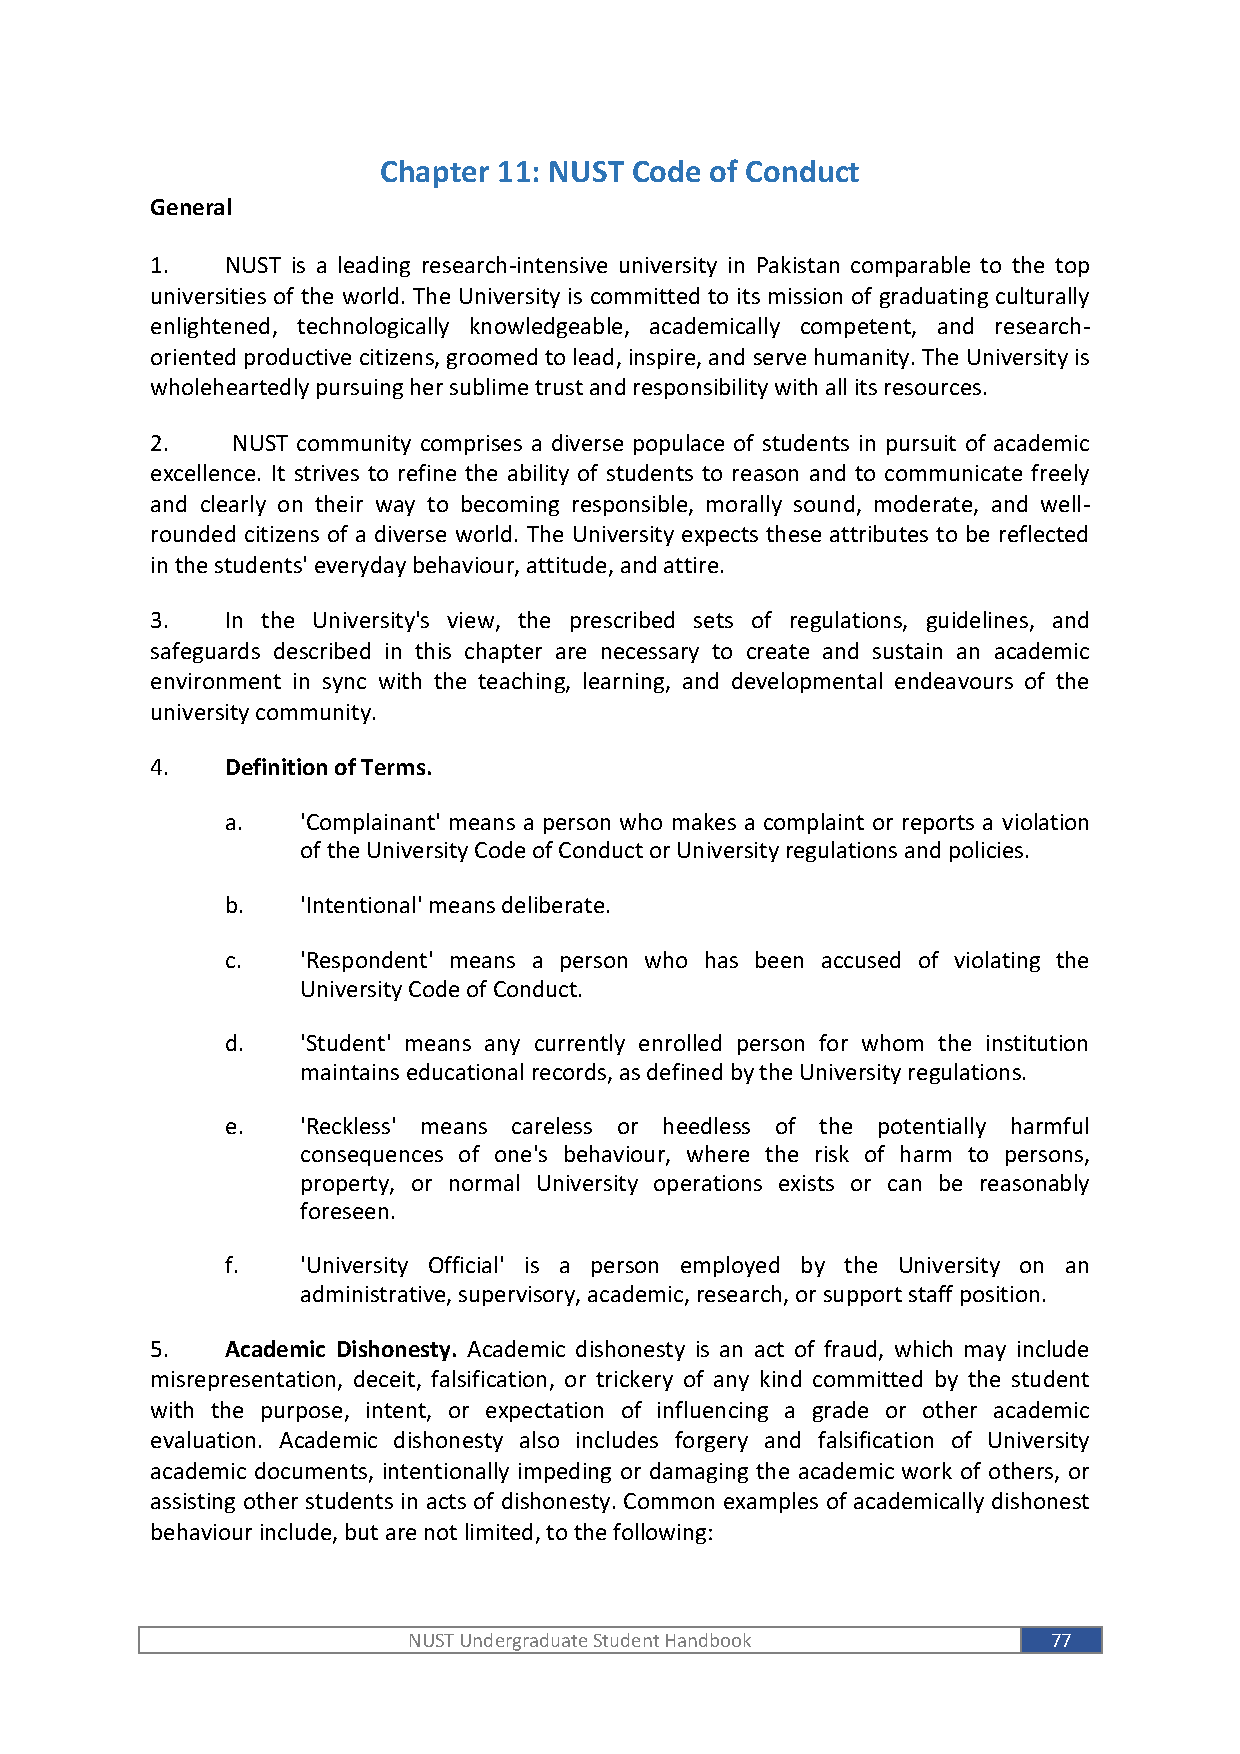
\includepdf[
  pages={1},
  scale=0.85,
  offset=0 -2.2cm,
  pagecommand={\thispagestyle{plain}\noindent{\Large\bfseries\thesection\quad Code of Conduct-UG Student Handbook}}
]{appendices/criterion_4/chapter-11.pdf}
\includepdf[
  pages={2-},
  pagecommand={\thispagestyle{plain}}
]{appendices/criterion_4/chapter-11.pdf}
%-------------------
\refstepcounter{section}
\phantomsection
\label{annex:D5}
\addcontentsline{toc}{section}{\protect\numberline{\thesection}Sample Student Feedback Report}
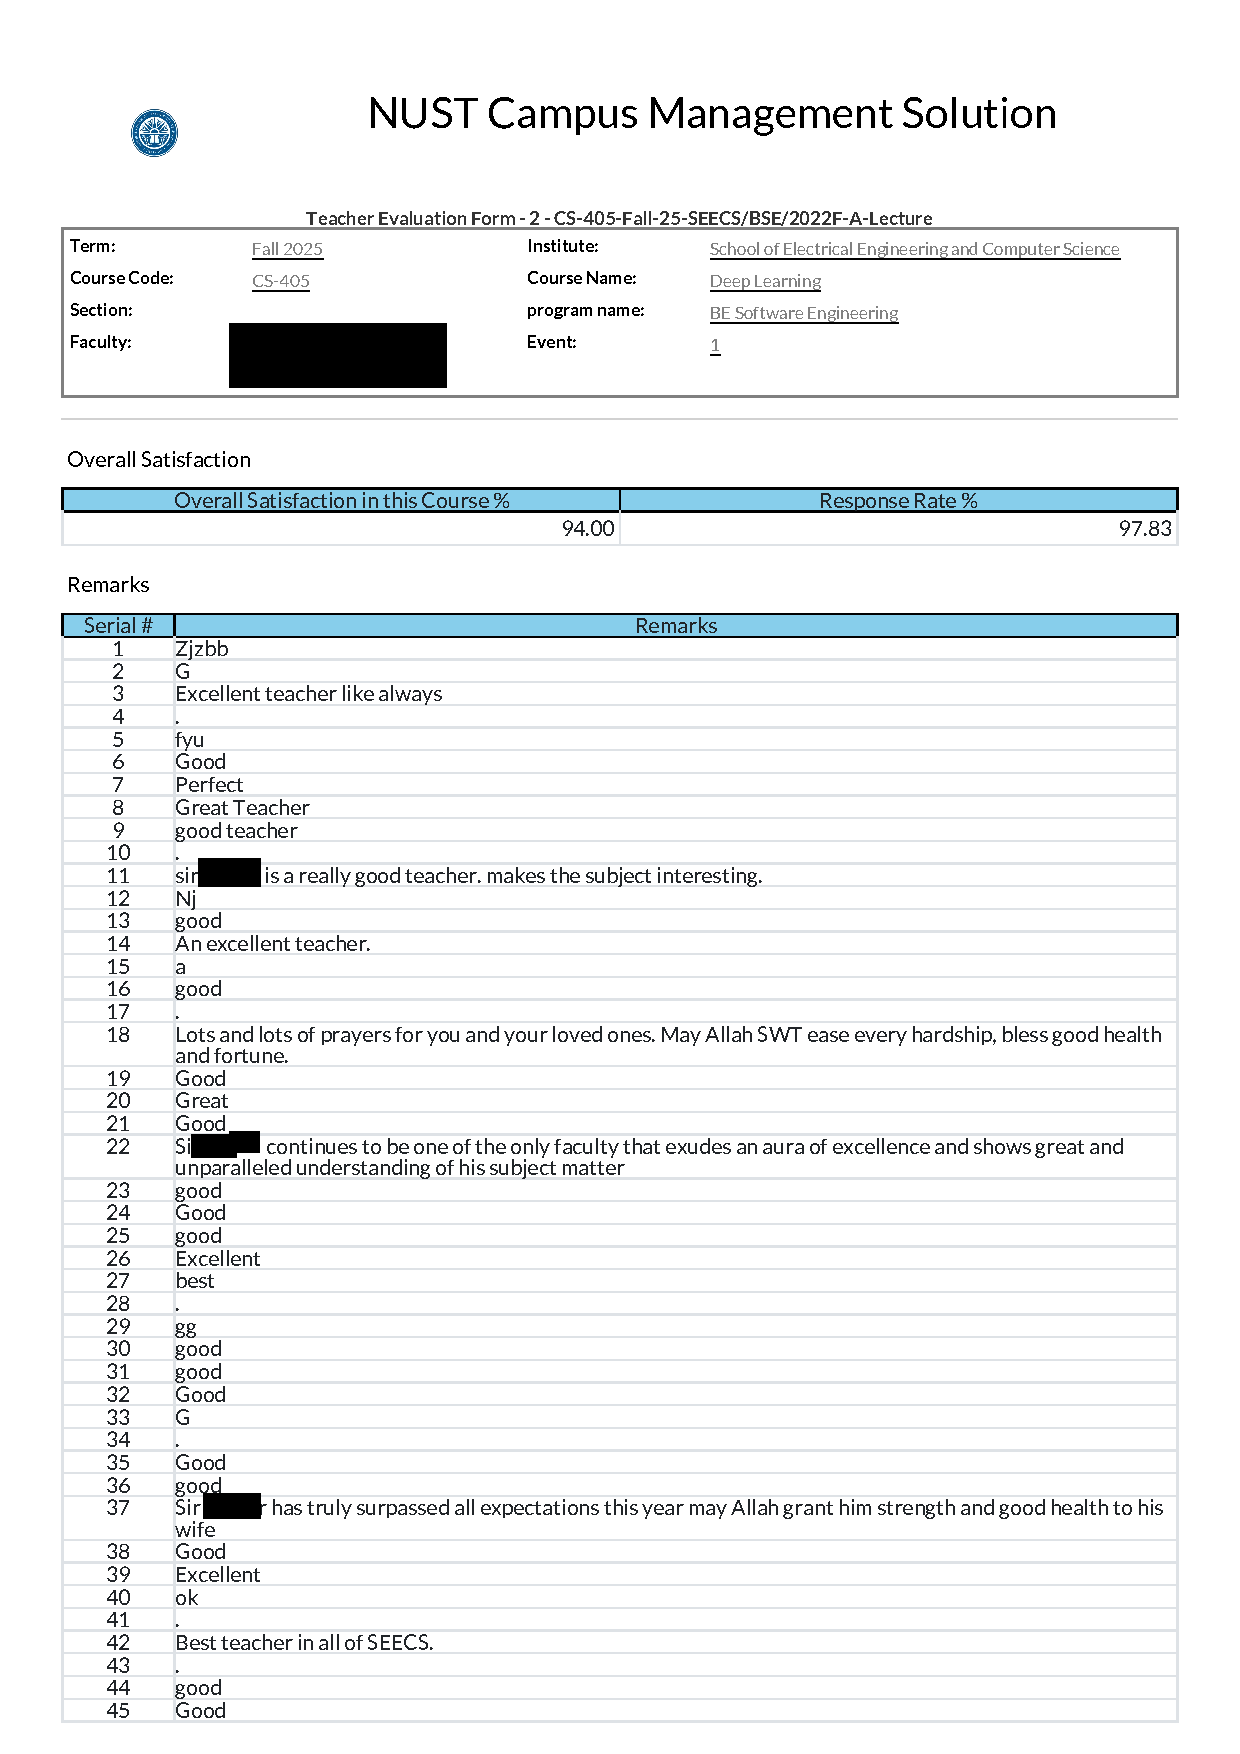
\includepdf[
  pages={1},
  scale=0.85,
  offset=0 -2.2cm,
  pagecommand={\thispagestyle{plain}\noindent{\Large\bfseries\thesection\quad Sample Student Feedback Report}}
]{appendices/criterion_4/Annex D5.pdf}
\includepdf[
  pages={2-},
  pagecommand={\thispagestyle{plain}}
]{appendices/criterion_4/Annex D5.pdf}

% ------------------------------------------------------------

\refstepcounter{section}
\phantomsection
\label{annex:D6}
\addcontentsline{toc}{section}{\protect\numberline{\thesection}Student Participation in International/National Events}
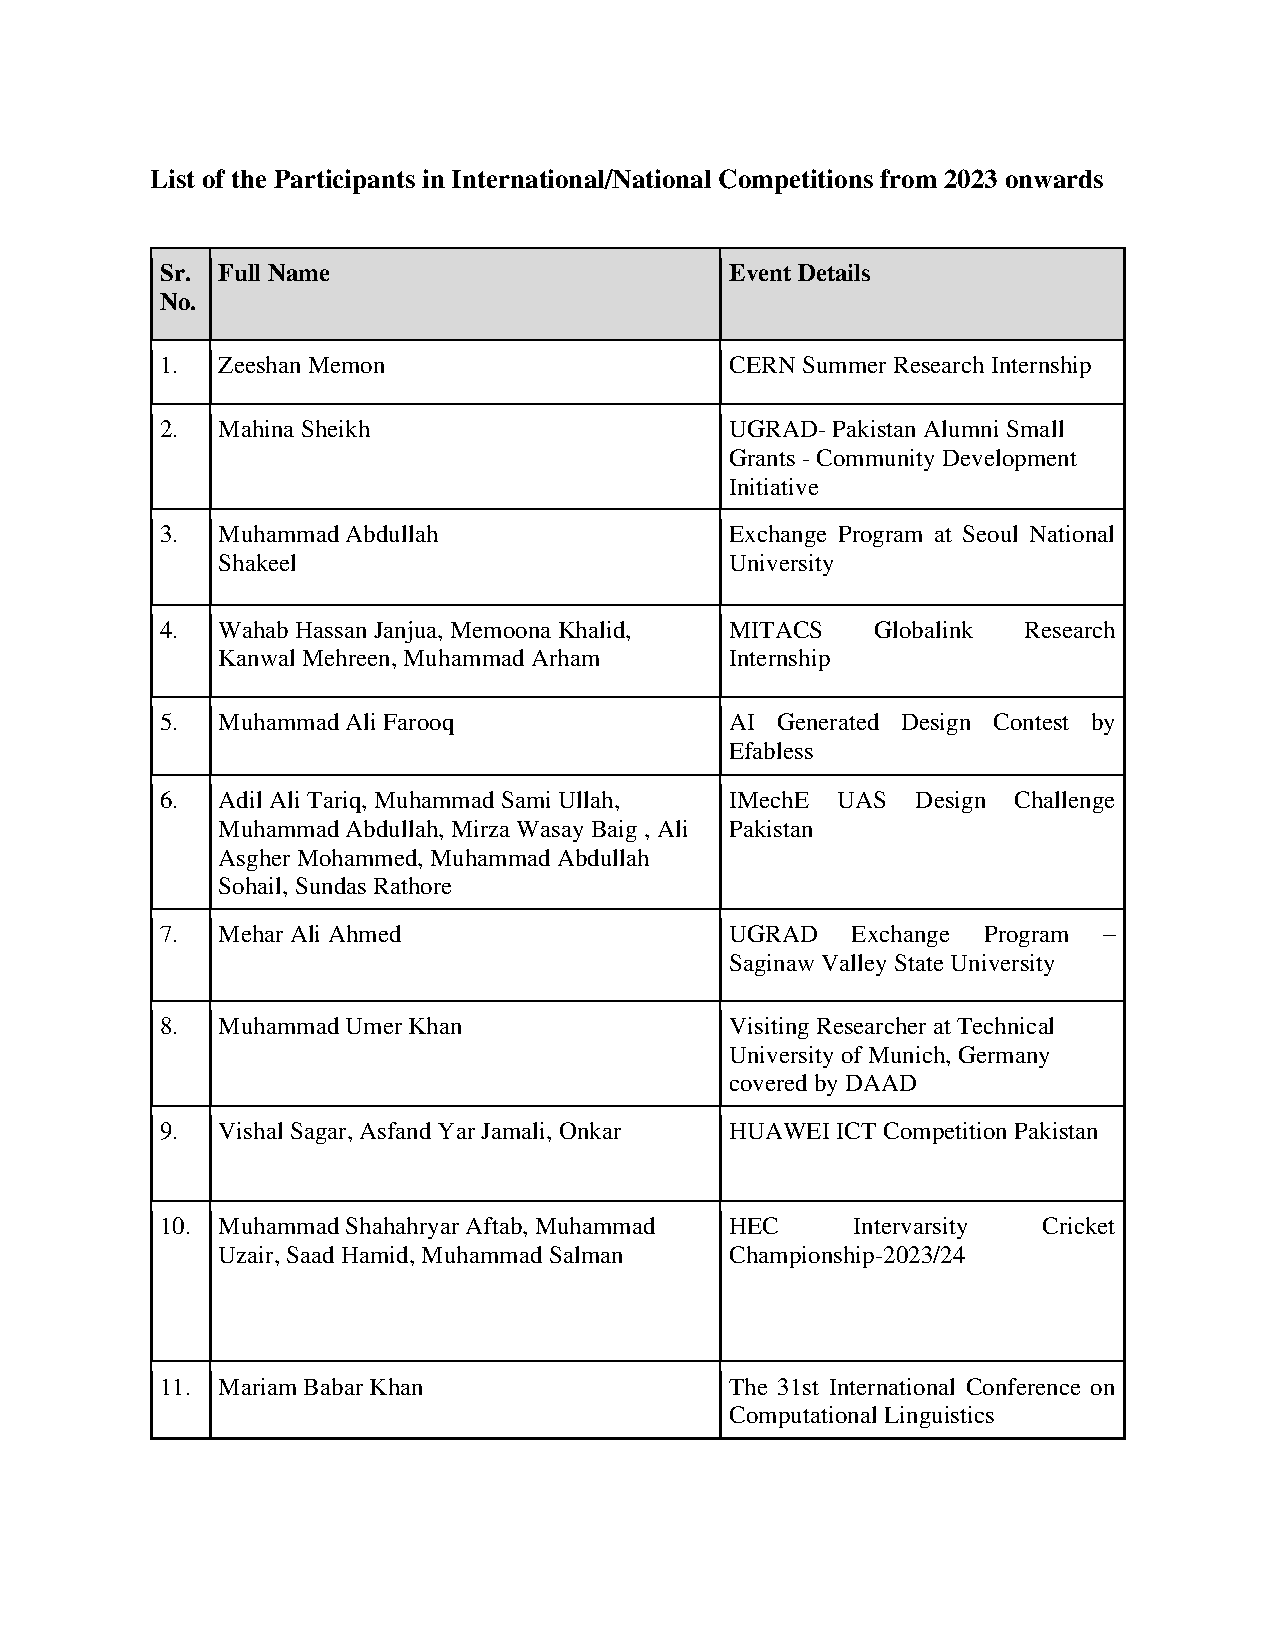
\includepdf[
  pages={1},
  scale=0.85,
  offset=0 -2.2cm,
  pagecommand={\thispagestyle{plain}\noindent{\Large\bfseries\thesection\quad Student Participation in International/National Events}}
]{appendices/criterion_4/Annex D6.pdf}
\includepdf[
  pages={2-},
  pagecommand={\thispagestyle{plain}}
]{appendices/criterion_4/Annex D6.pdf}
%------------------------
\refstepcounter{section}
\phantomsection
\label{annex:D7}
\addcontentsline{toc}{section}{\protect\numberline{\thesection}Community Service Learning Course Outline}
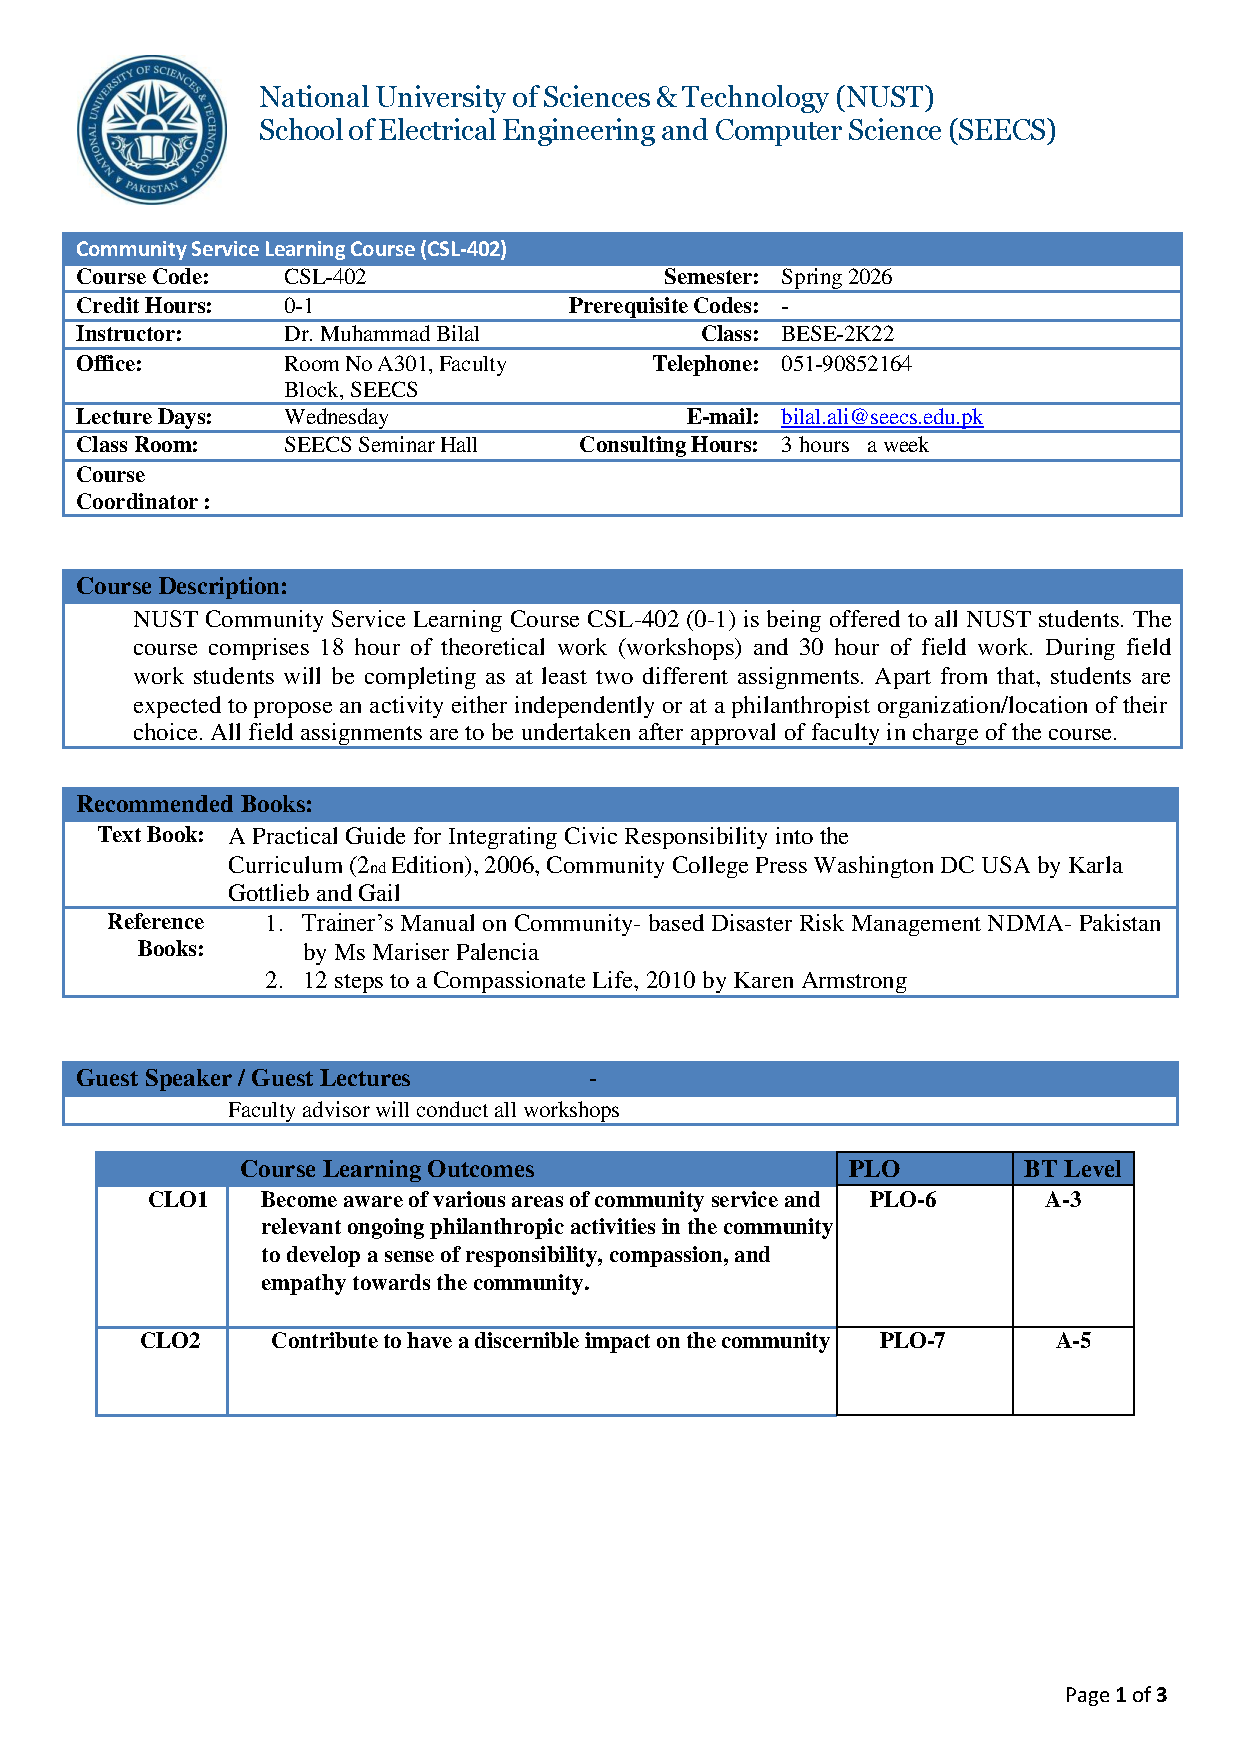
\includepdf[
  pages={1},
  scale=0.85,
  offset=0 -2.2cm,
  pagecommand={\thispagestyle{plain}\noindent{\Large\bfseries\thesection\quad Community Service Learning Course Outline}}
]{appendices/criterion_4/Annex D9.pdf}
\includepdf[
  pages={2-},
  pagecommand={\thispagestyle{plain}}
]{appendices/criterion_4/Annex D9.pdf}


% ------------------------------------------------------------

\refstepcounter{section}
\phantomsection
\label{annex:D10}
\addcontentsline{toc}{section}{\protect\numberline{\thesection}Details of Students receiving Scholarships}
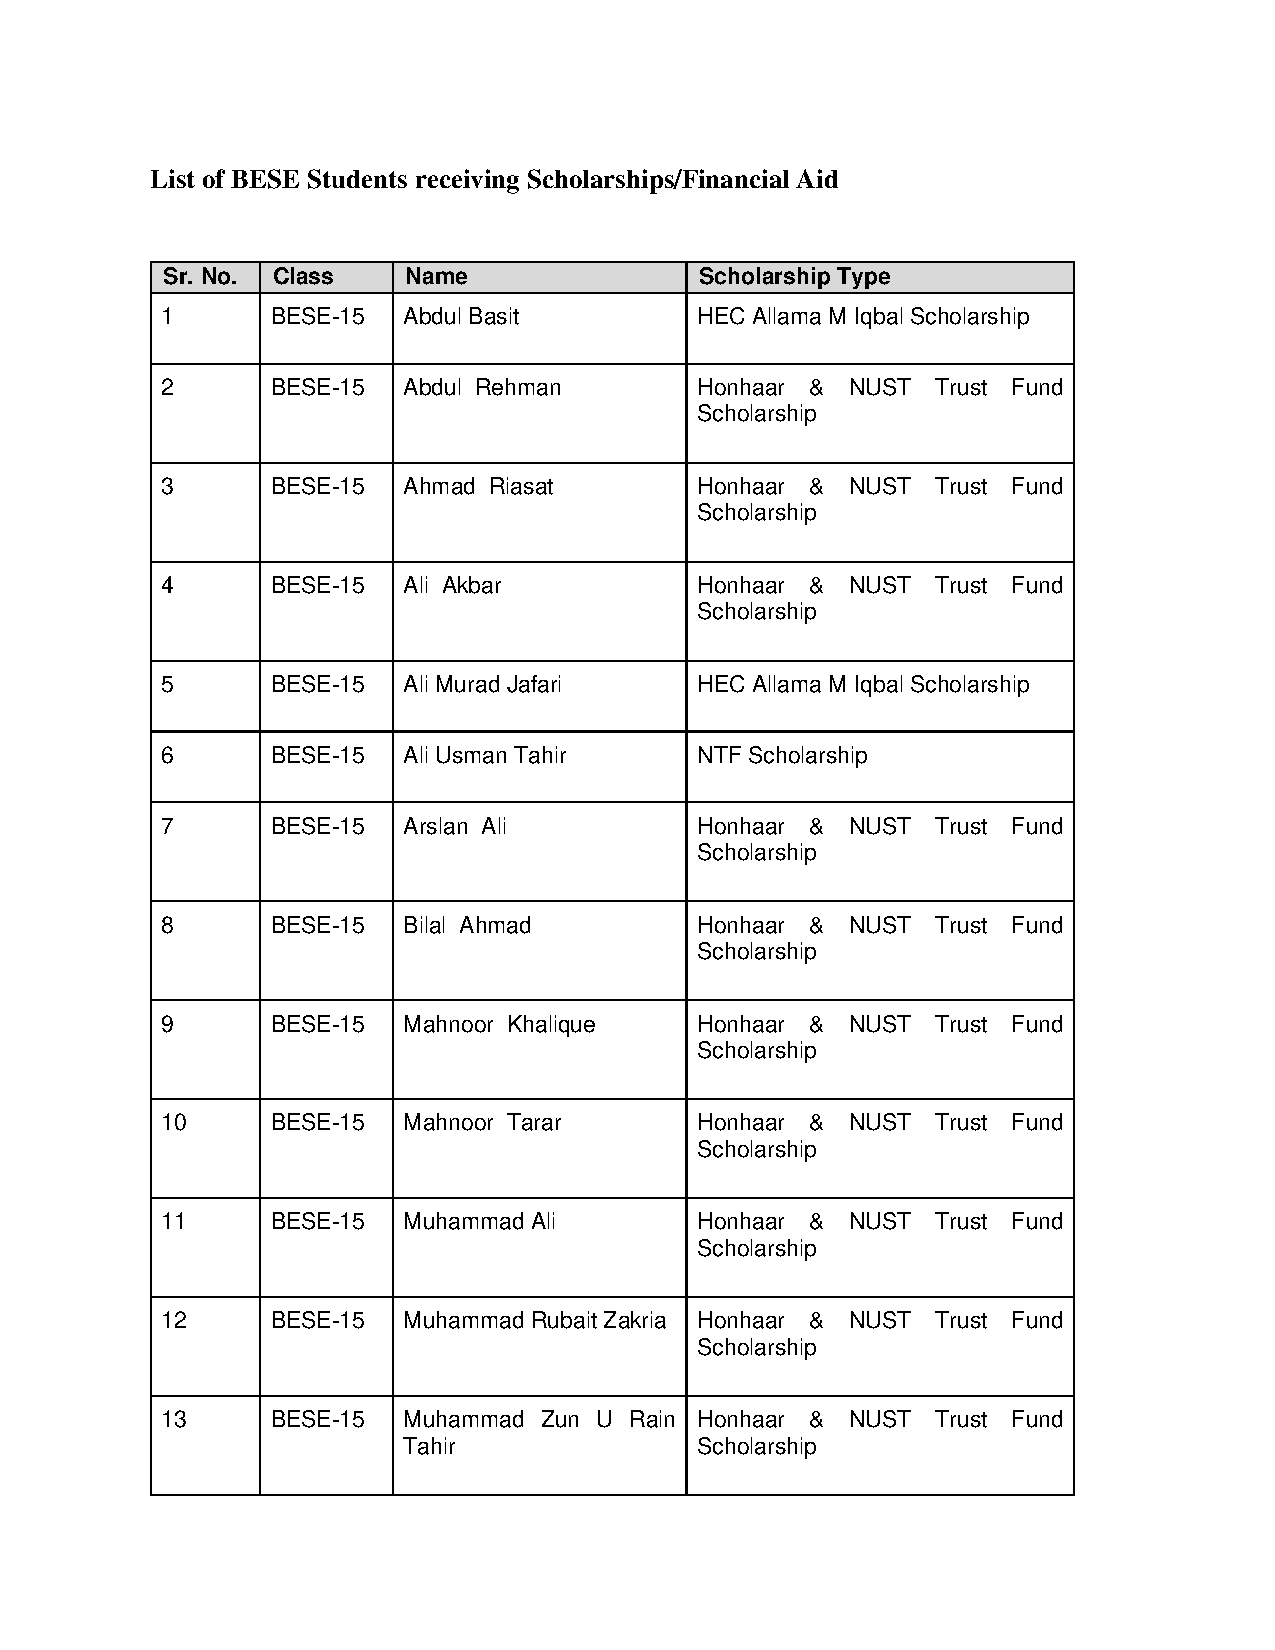
\includepdf[
  pages={1},
  scale=0.85,
  offset=0 -2.2cm,
  pagecommand={\thispagestyle{plain}\noindent{\Large\bfseries\thesection\quad Details of Students receiving Scholarships}}
]{appendices/criterion_4/Annex D10.pdf}
\includepdf[
  pages={2-},
  pagecommand={\thispagestyle{plain}}
]{appendices/criterion_4/Annex D10.pdf}

% ------------------------------------------------------------

\refstepcounter{section}
\phantomsection
\label{annex:D11}
\addcontentsline{toc}{section}{\protect\numberline{\thesection}International Universities hosting NUST Students for Semester Exchange}
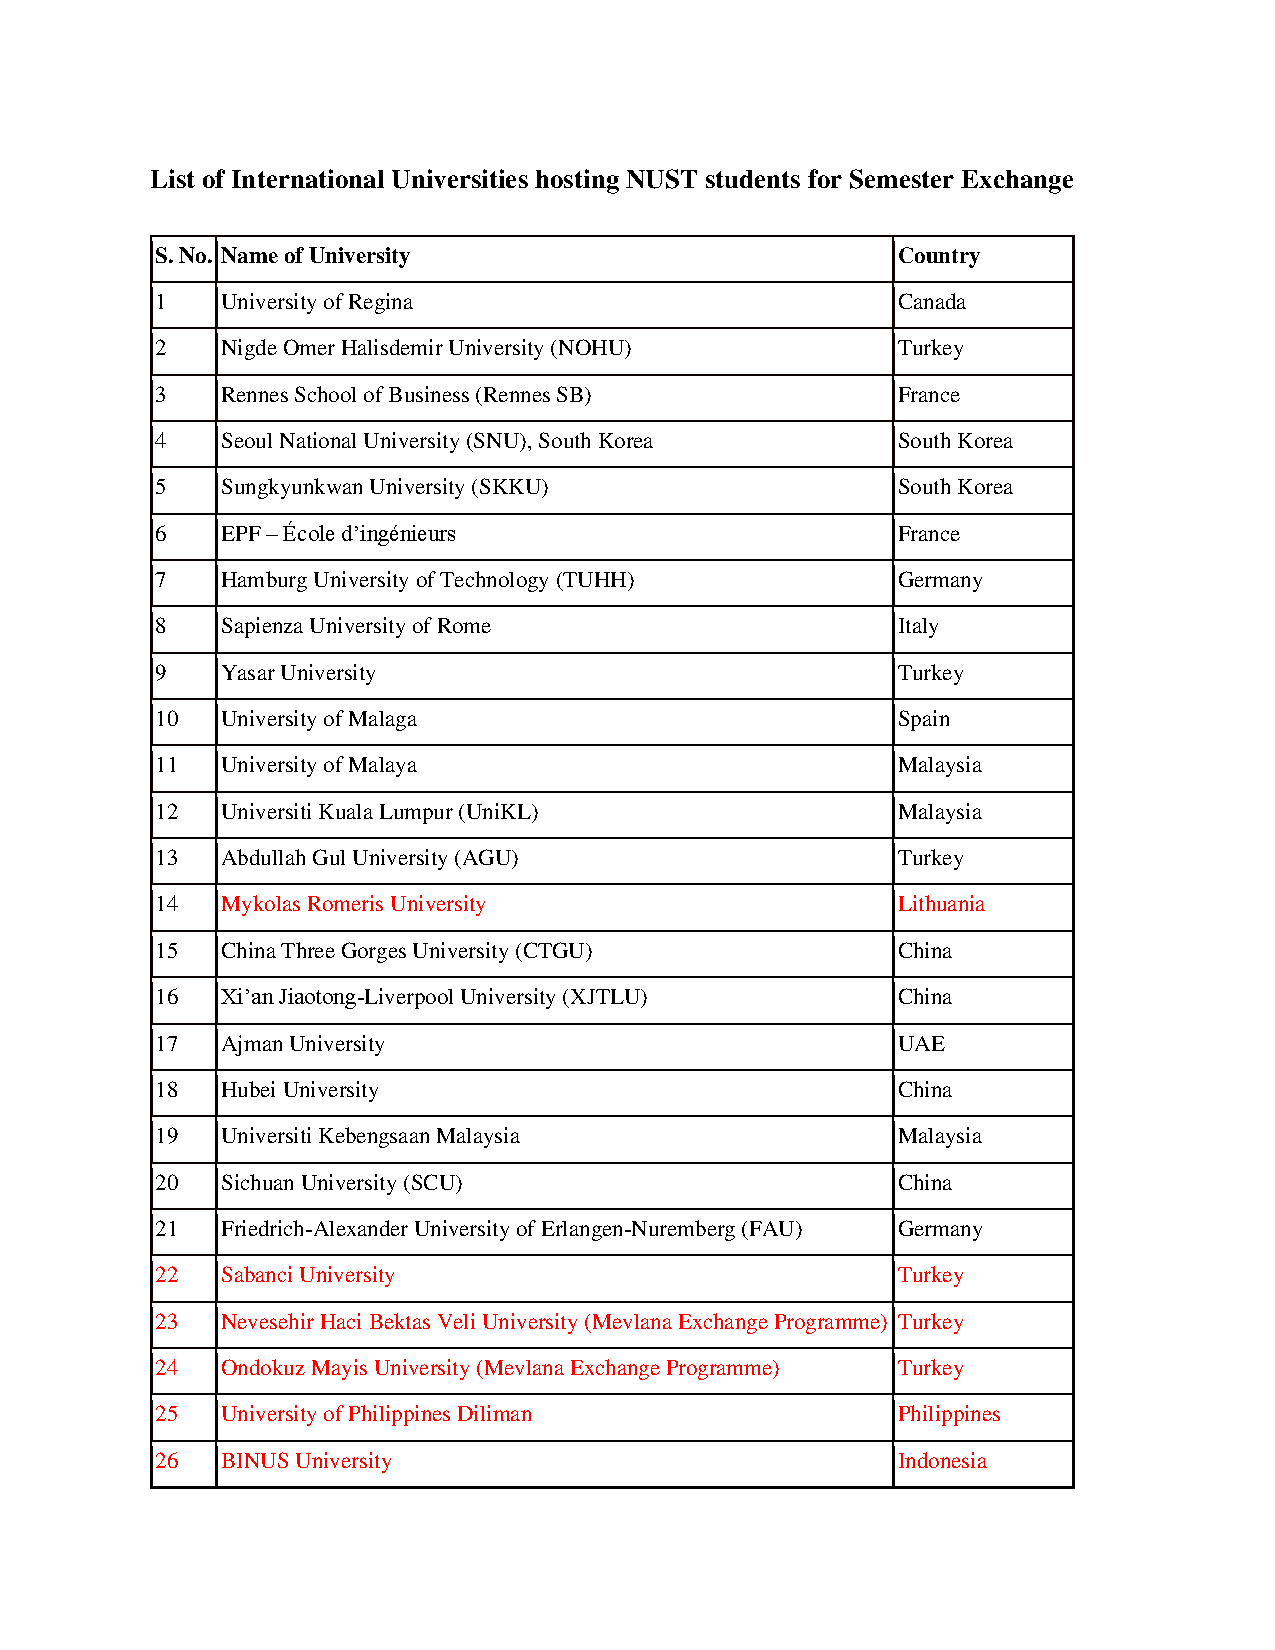
\includepdf[
  pages={1},
  scale=0.85,
  offset=0 -2.2cm,
  pagecommand={\thispagestyle{plain}\noindent{\Large\bfseries\thesection\quad International Universities hosting NUST Students for Semester Exchange}}
]{appendices/criterion_4/Annex D11.pdf}
\includepdf[
  pages={2-},
  pagecommand={\thispagestyle{plain}}
]{appendices/criterion_4/Annex D11.pdf}

\clearpage
\clearpage
\setcounter{section}{0}
\renewcommand{\thesection}{E.\arabic{section}}
\renewcommand{\theHsection}{annexE.\arabic{section}}

\phantomsection
\addcontentsline{toc}{chapter}{Annexure E: Criteria 5 Supporting Documents}
\label{app:criteria-5}

\refstepcounter{section}
\phantomsection
\label{annex:AG}
\addcontentsline{toc}{section}{\protect\numberline{\thesection}NUST Statutes VI - Faculty Duties and Responsibilities}

% ---- Heading block defined as a (long) macro, so \par is allowed ----
\newcommand{\annexEFirstPageHead}{%
  \noindent{\Huge\bfseries Annexure E: Criteria 5 Supporting Documents}\par
  \vspace{0.8em}
  \noindent Here we provide the supporting annexures required for Criterion 5: Faculty and Support Staff.\par
  \vspace{0.8em}
  \noindent{\Large\bfseries\thesection\quad 
  NUST Statutes VI - Faculty Duties and Responsibilities}\par
}

% ---- Page 1: heading + shrunk PDF page ----
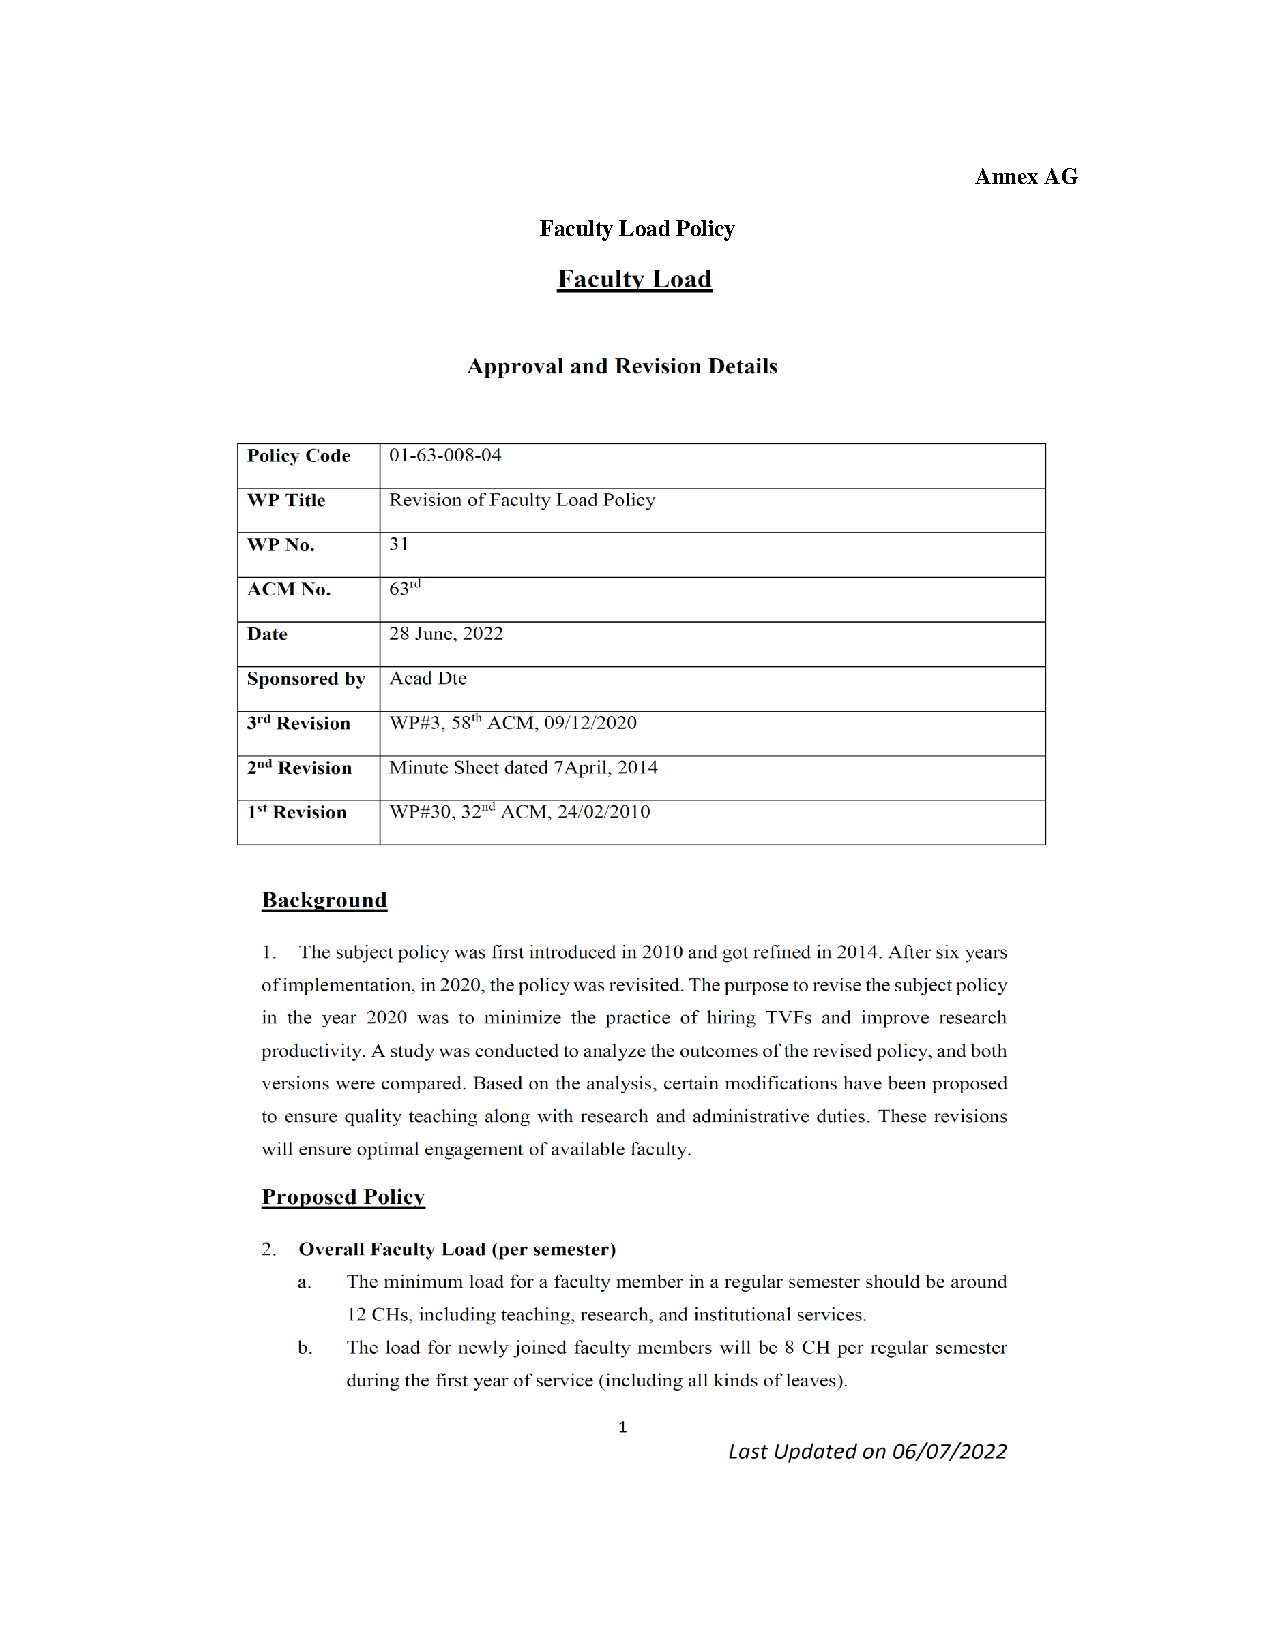
\includepdf[
  pages={1},
  scale=0.85,
  offset=0 -2.2cm,
  pagecommand={\thispagestyle{plain}\annexEFirstPageHead}
]{appendices/criterion_5/Annex E1.pdf}

% ---- Pages 2 to end: unchanged ----
\includepdf[
  pages={2-},
  pagecommand={\thispagestyle{plain}}
]{appendices/criterion_5/Annex E1.pdf}
%==================================================
% ------------------------------------------------------------
\refstepcounter{section}
\phantomsection
\label{annex:I}
\addcontentsline{toc}{section}{\protect\numberline{\thesection}Faculty Qualifications, Experience and Specialties}
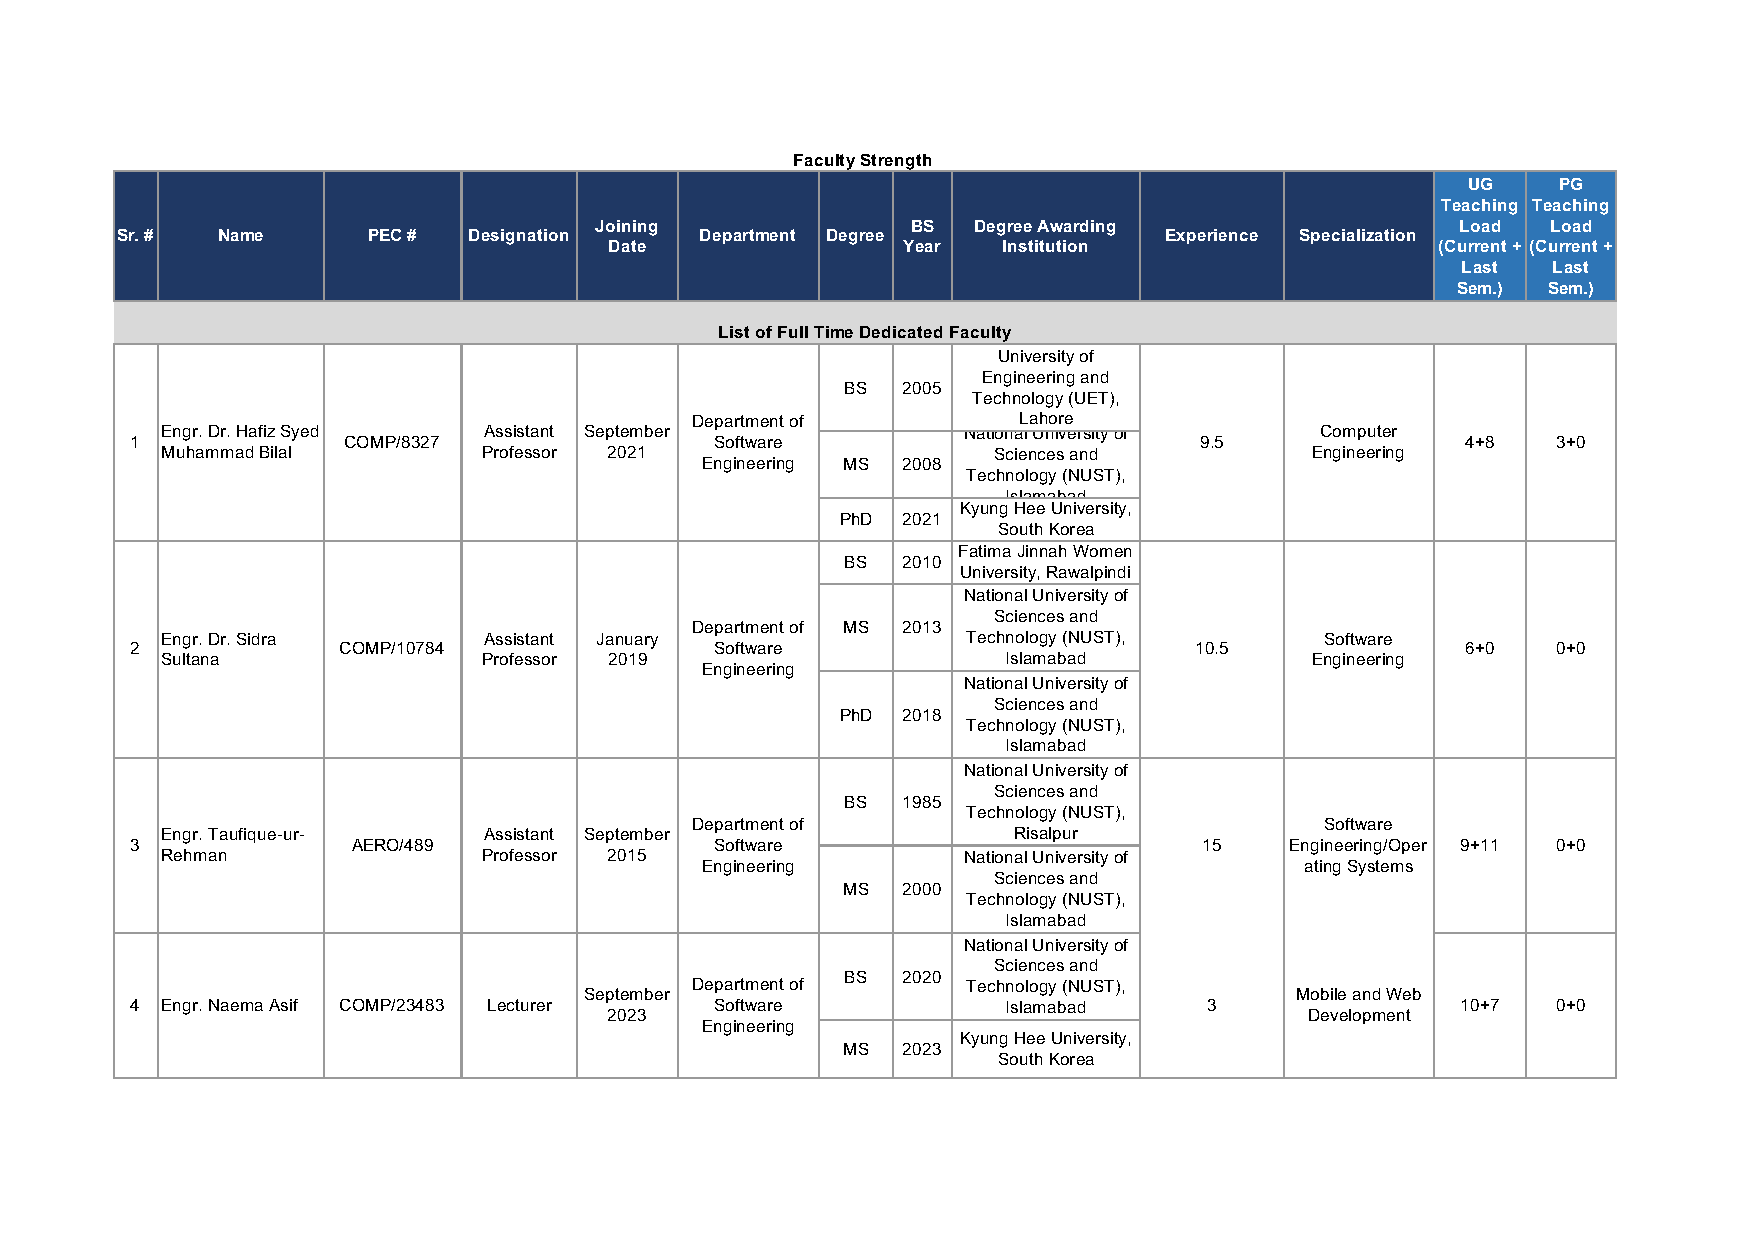
\includepdf[
  pages={1},
  scale=0.90,
  offset=0 -2.2cm,
  landscape,
  pagecommand={\thispagestyle{plain}\noindent{\Large\bfseries\thesection\quad Faculty Qualifications, Experience and Specialties}}
]{appendices/criterion_5/Annex-II-fin.pdf}

% ---- Pages 2 to end: unchanged ----
\includepdf[
  pages={2-},
  landscape,
  pagecommand={\thispagestyle{plain}}
]{appendices/criterion_5/Annex-II-fin.pdf}
% ------------------------------------------------------------
 
\refstepcounter{section}
\phantomsection
\label{annex:J}
\addcontentsline{toc}{section}{\protect\numberline{\thesection}Summary of Software Engineering Faculty}
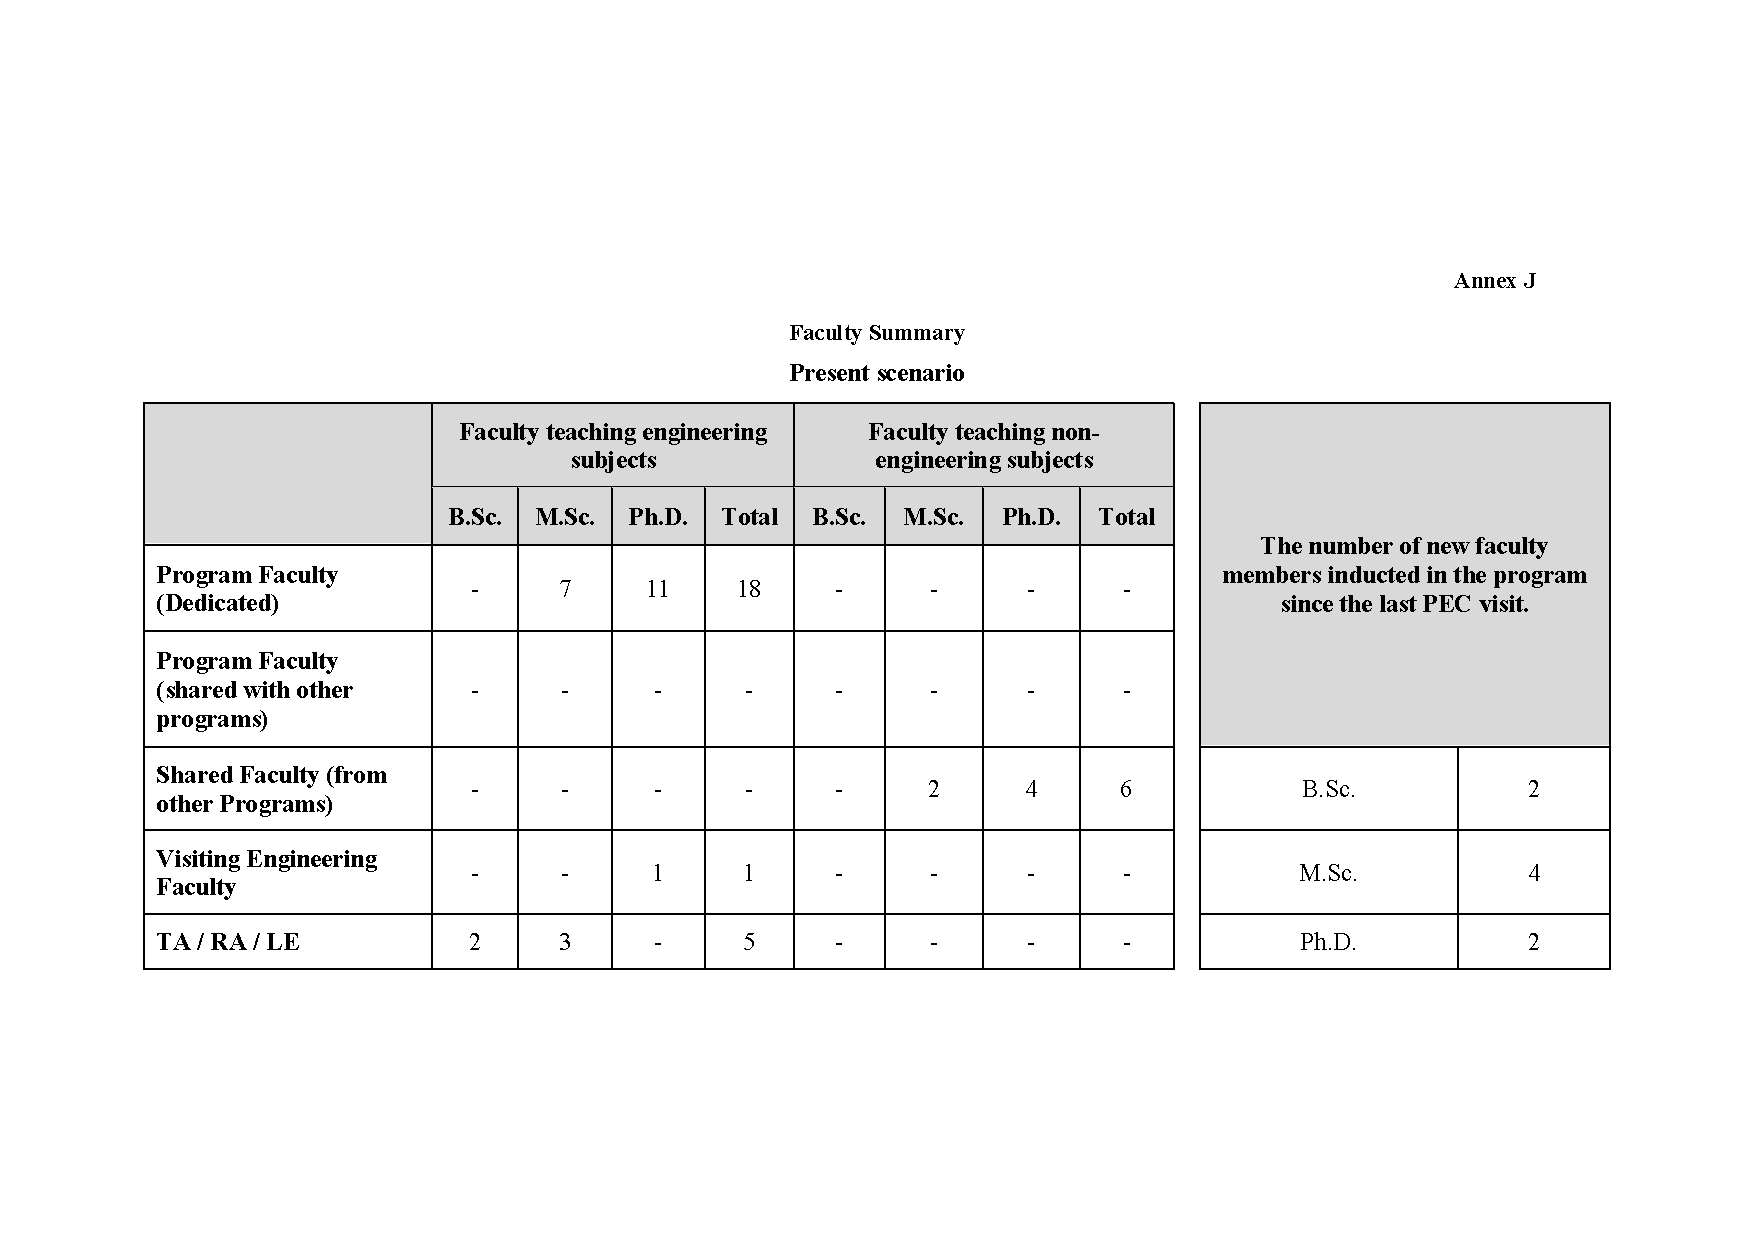
\includepdf[
  pages={1},
  scale=0.90,
  landscape,
  offset=0 -2.2cm,
  pagecommand={\thispagestyle{plain}\noindent{\Large\bfseries\thesection\quad Summary of Software Engineering Faculty}}
]{appendices/criterion_5/Annex J.pdf}

% ---- Pages 2 to end: unchanged ----
\includepdf[
  pages={2-},
  landscape,
  pagecommand={\thispagestyle{plain}}
]{appendices/criterion_5/Annex J.pdf}
% ------------------------------------------------------------

\refstepcounter{section}
\phantomsection
\label{annex:K}
\addcontentsline{toc}{section}{\protect\numberline{\thesection}Credit Hours and Faculty Workload Details}
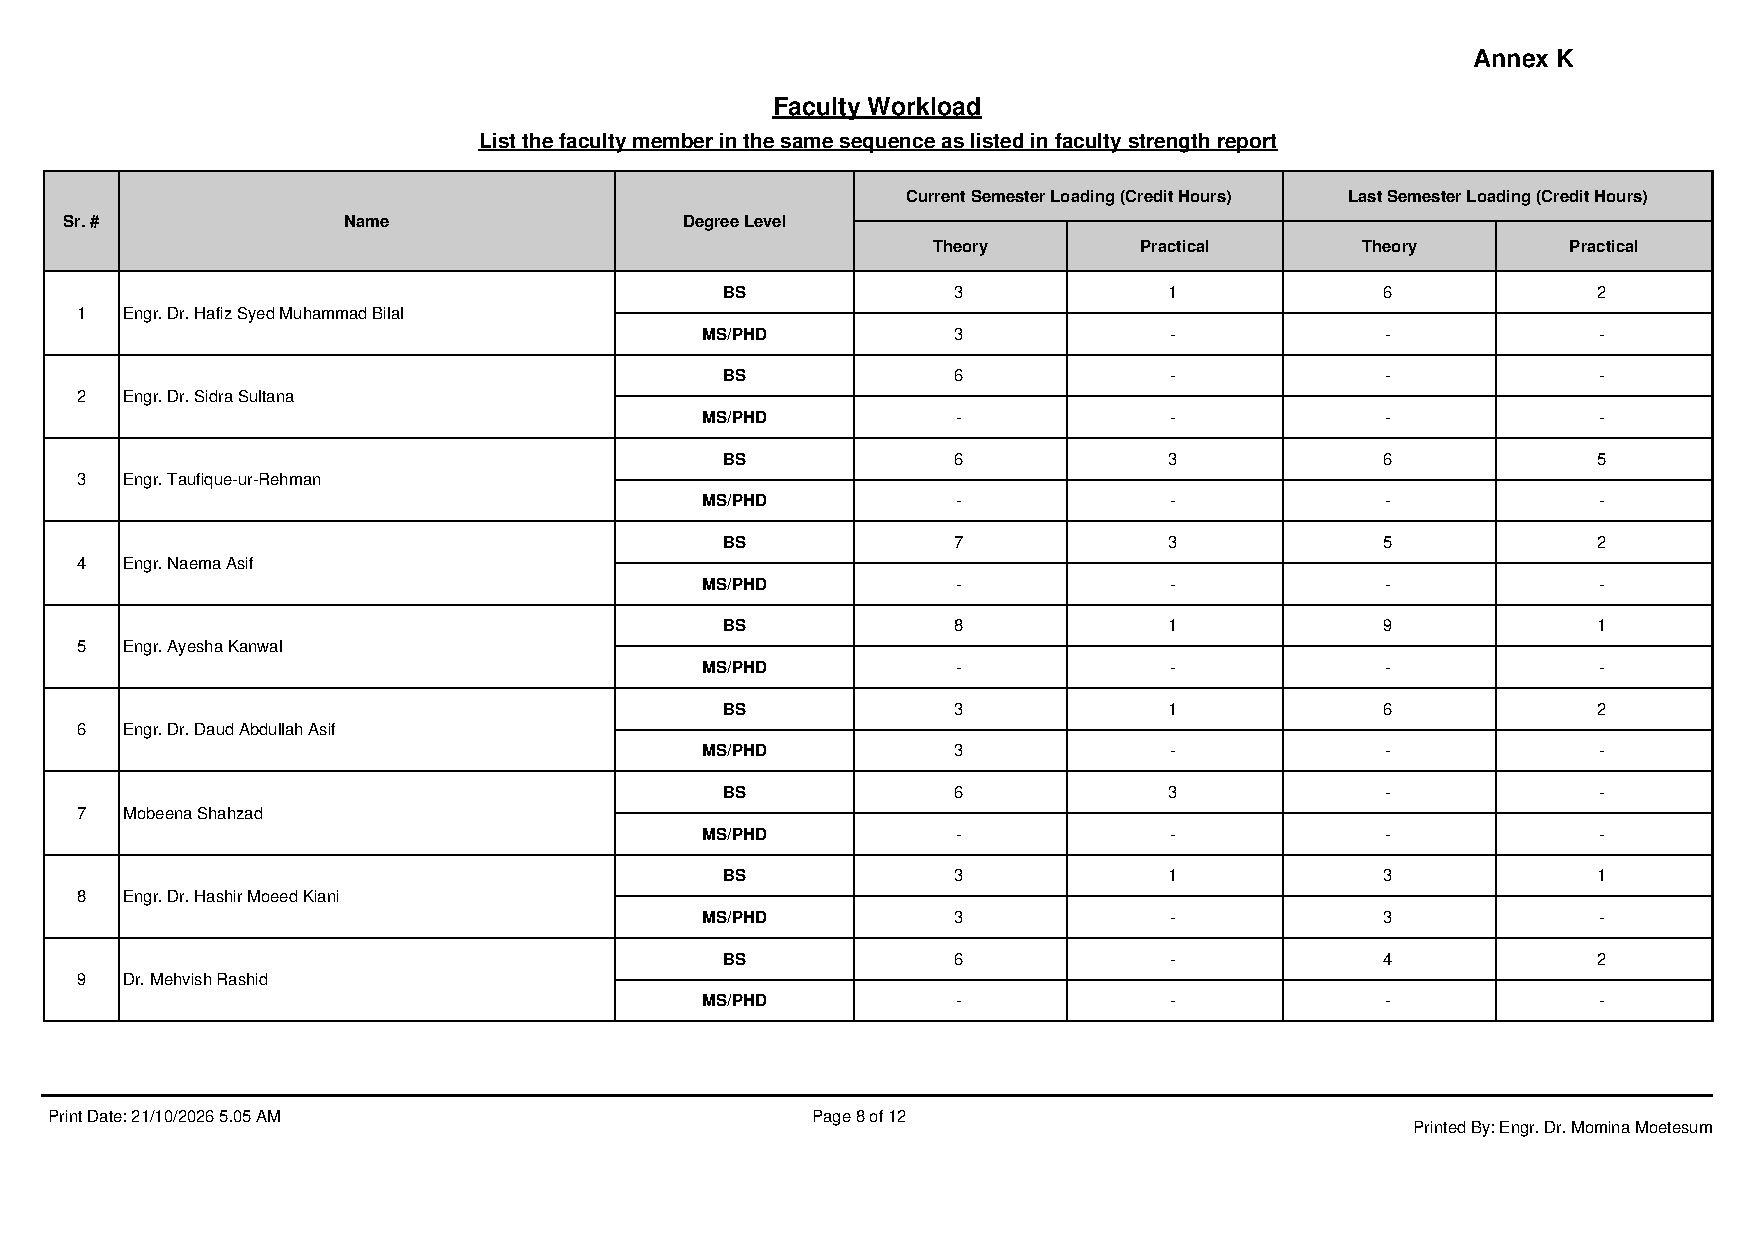
\includepdf[
 pages={1},
 scale=0.90,
 offset=0 -2.2cm,
 landscape,
 pagecommand={\thispagestyle{plain}\noindent{\Large\bfseries\thesection\quad Credit Hours and Faculty Workload Details}}
]{appendices/criterion_5/workload.pdf}
\includepdf[
  pages={2-},
  landscape,
  pagecommand={\thispagestyle{plain}}
]{appendices/criterion_5/workload.pdf}
% ------------------------------------------------------------
\refstepcounter{section}
\phantomsection
\label{annex:T}
\addcontentsline{toc}{section}{\protect\numberline{\thesection}Recently Conducted OBE Trainings}
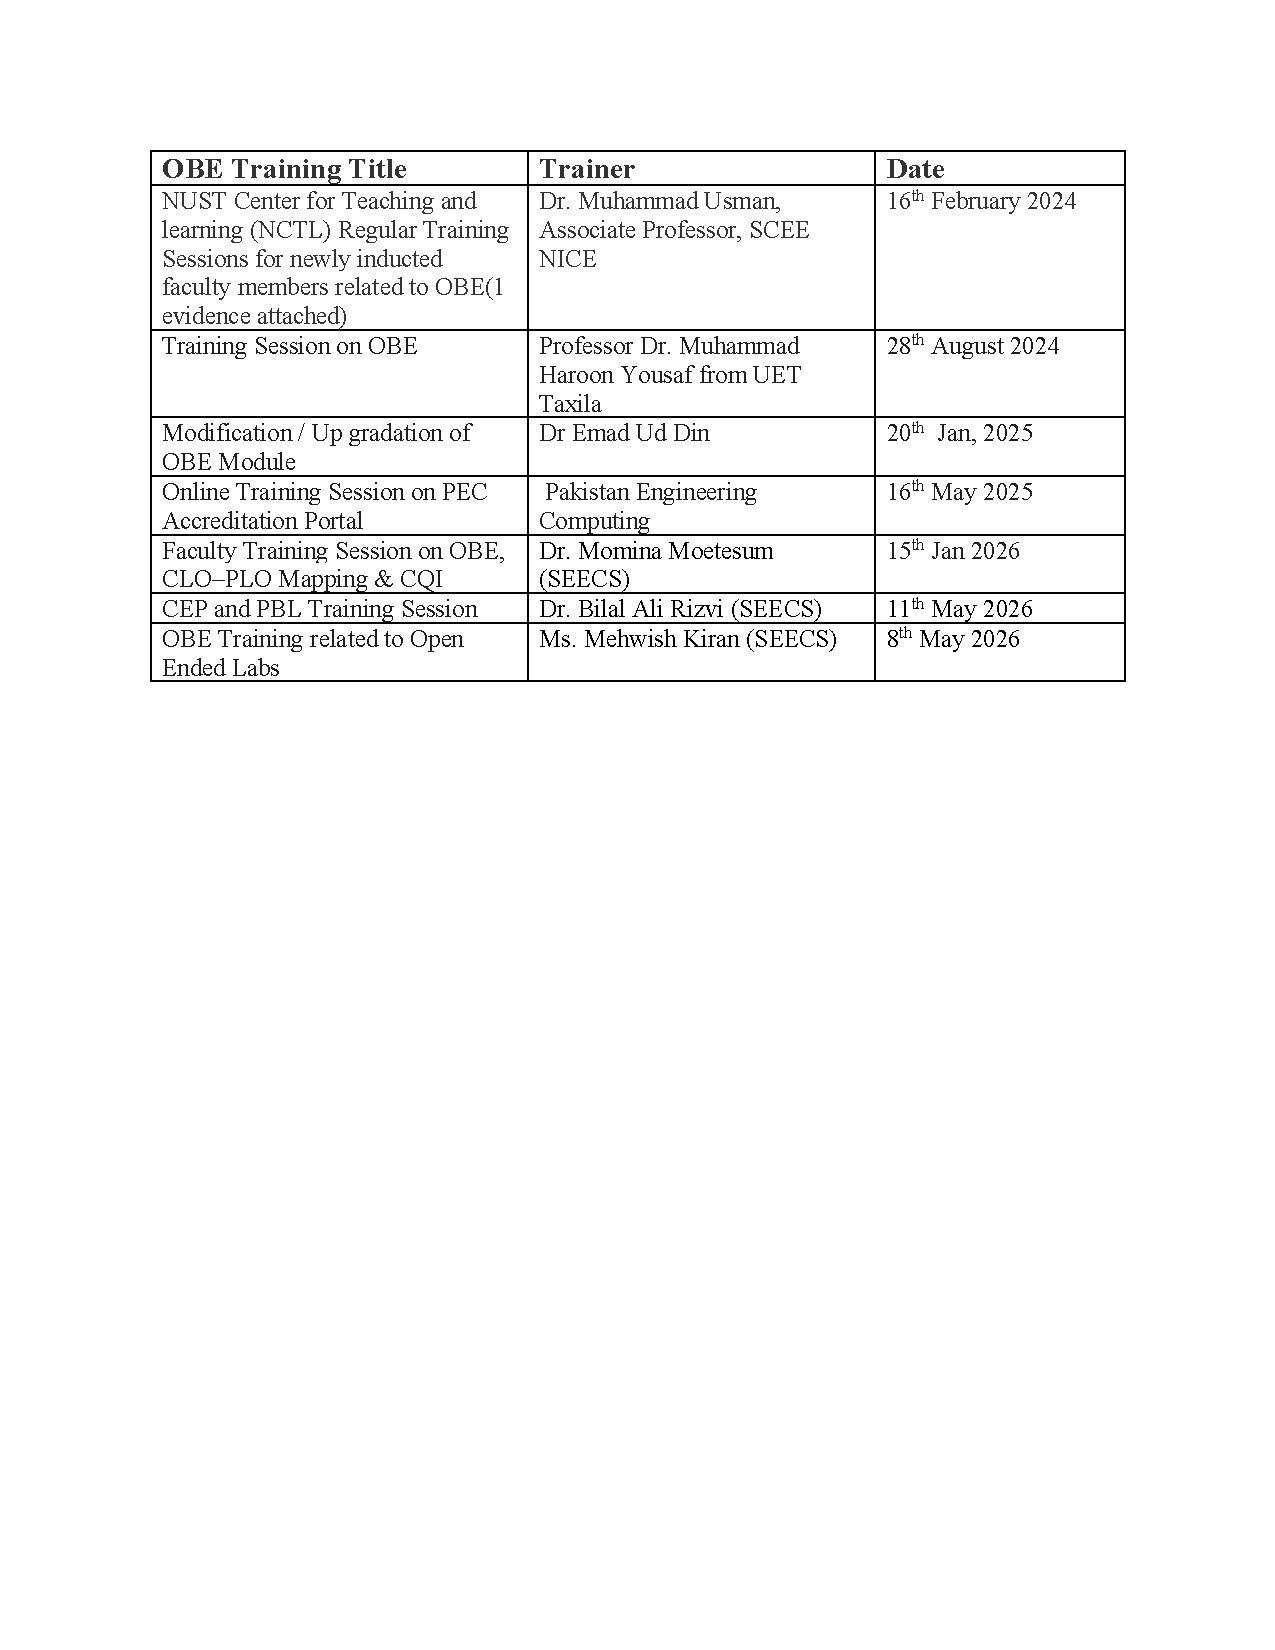
\includepdf[
  pages={1},
  scale=0.90,
  offset=0 -2.2cm,
  pagecommand={\thispagestyle{plain}\noindent{\Large\bfseries\thesection\quad Recently Conducted OBE Trainings}}
]{appendices/criterion_5/OBE-trainings.pdf}

%\refstepcounter{section}
%\phantomsection
%\label{annex:M}
%\addcontentsline{toc}{section}{\protect\numberline{\thesection}PEC Registered FTDF Members}
%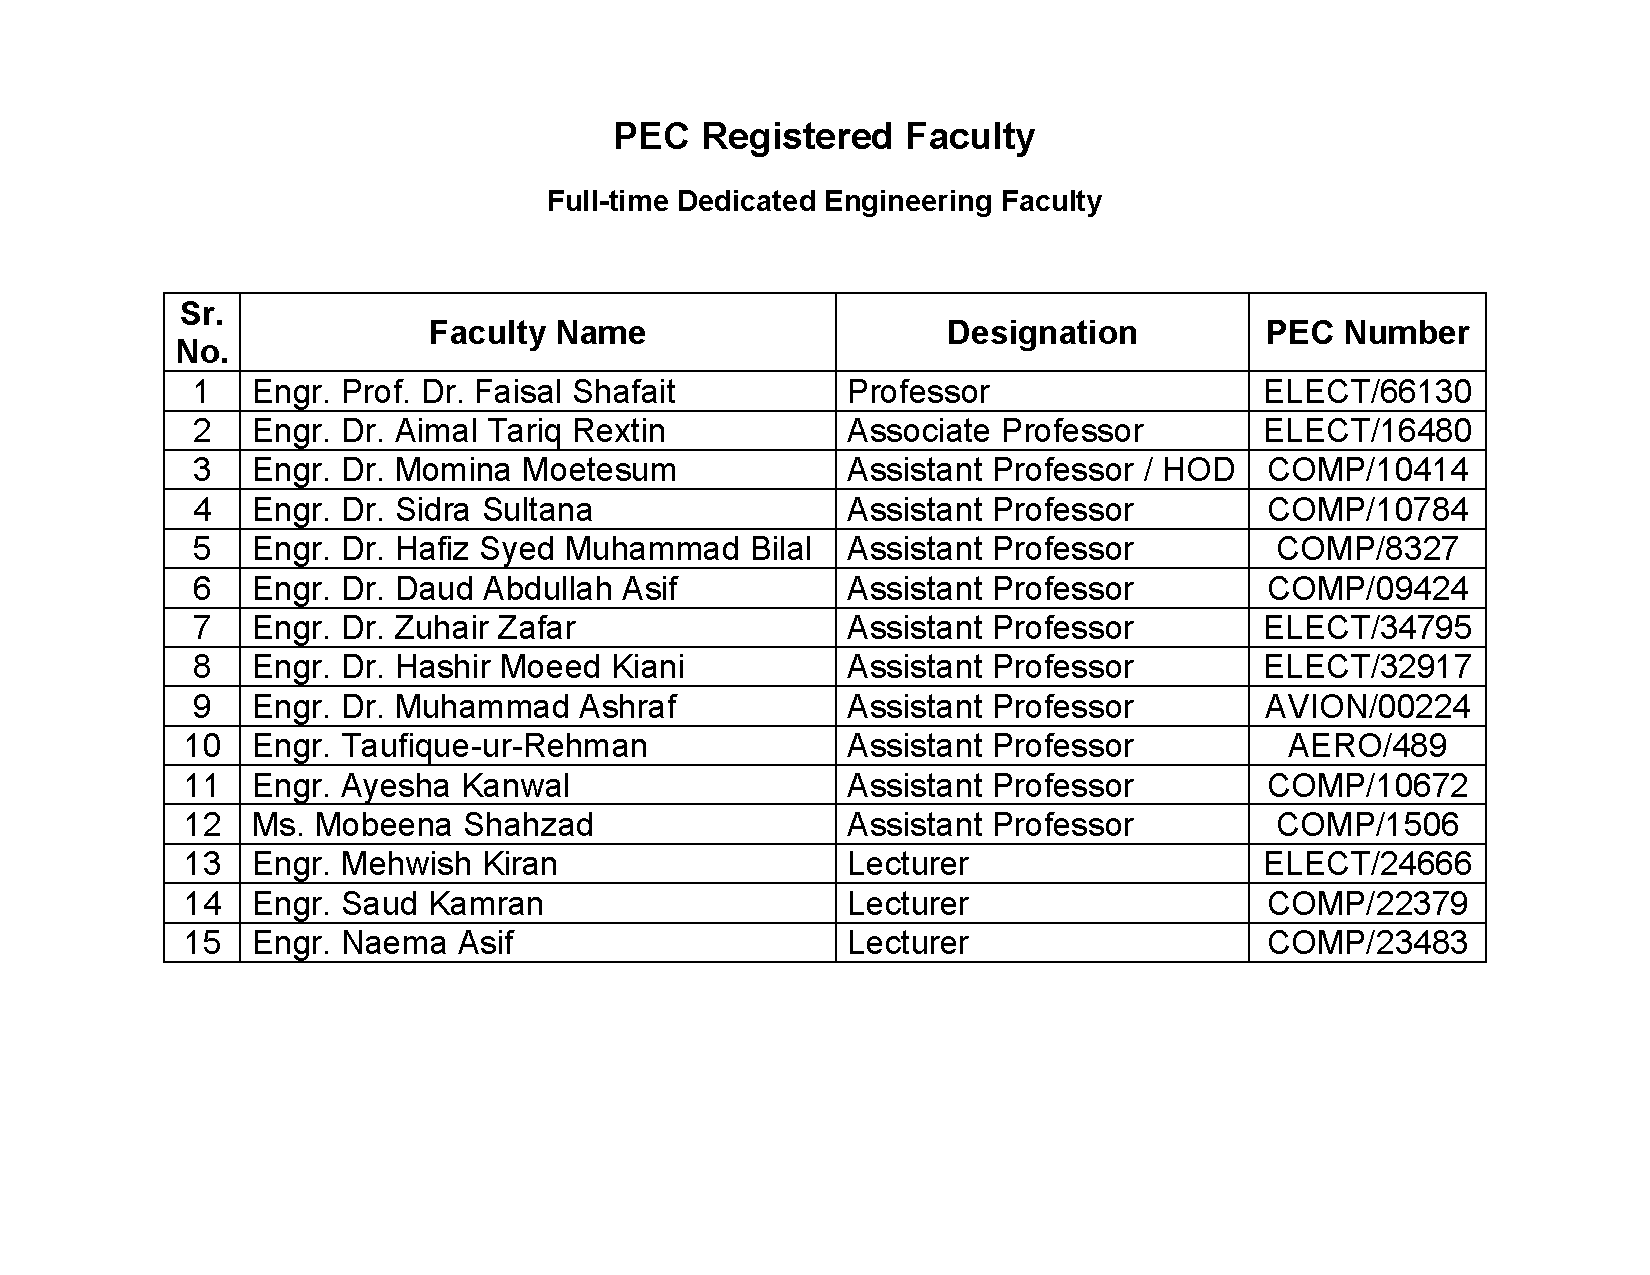
\includepdf[
%  pages={-},
%  scale=0.90,
%  offset=0 -1.2cm,
%  pagecommand={\thispagestyle{plain}\noindent{\Large\bfseries\thesection\quad PEC Registered Faculty Members}}
%]{appendices/criterion_5/pec-faculty.pdf}

%----------------------
\refstepcounter{section}
\phantomsection
\label{annex:r}
\addcontentsline{toc}{section}{\protect\numberline{\thesection}Google Scholar Profiles of FTDF of SE}
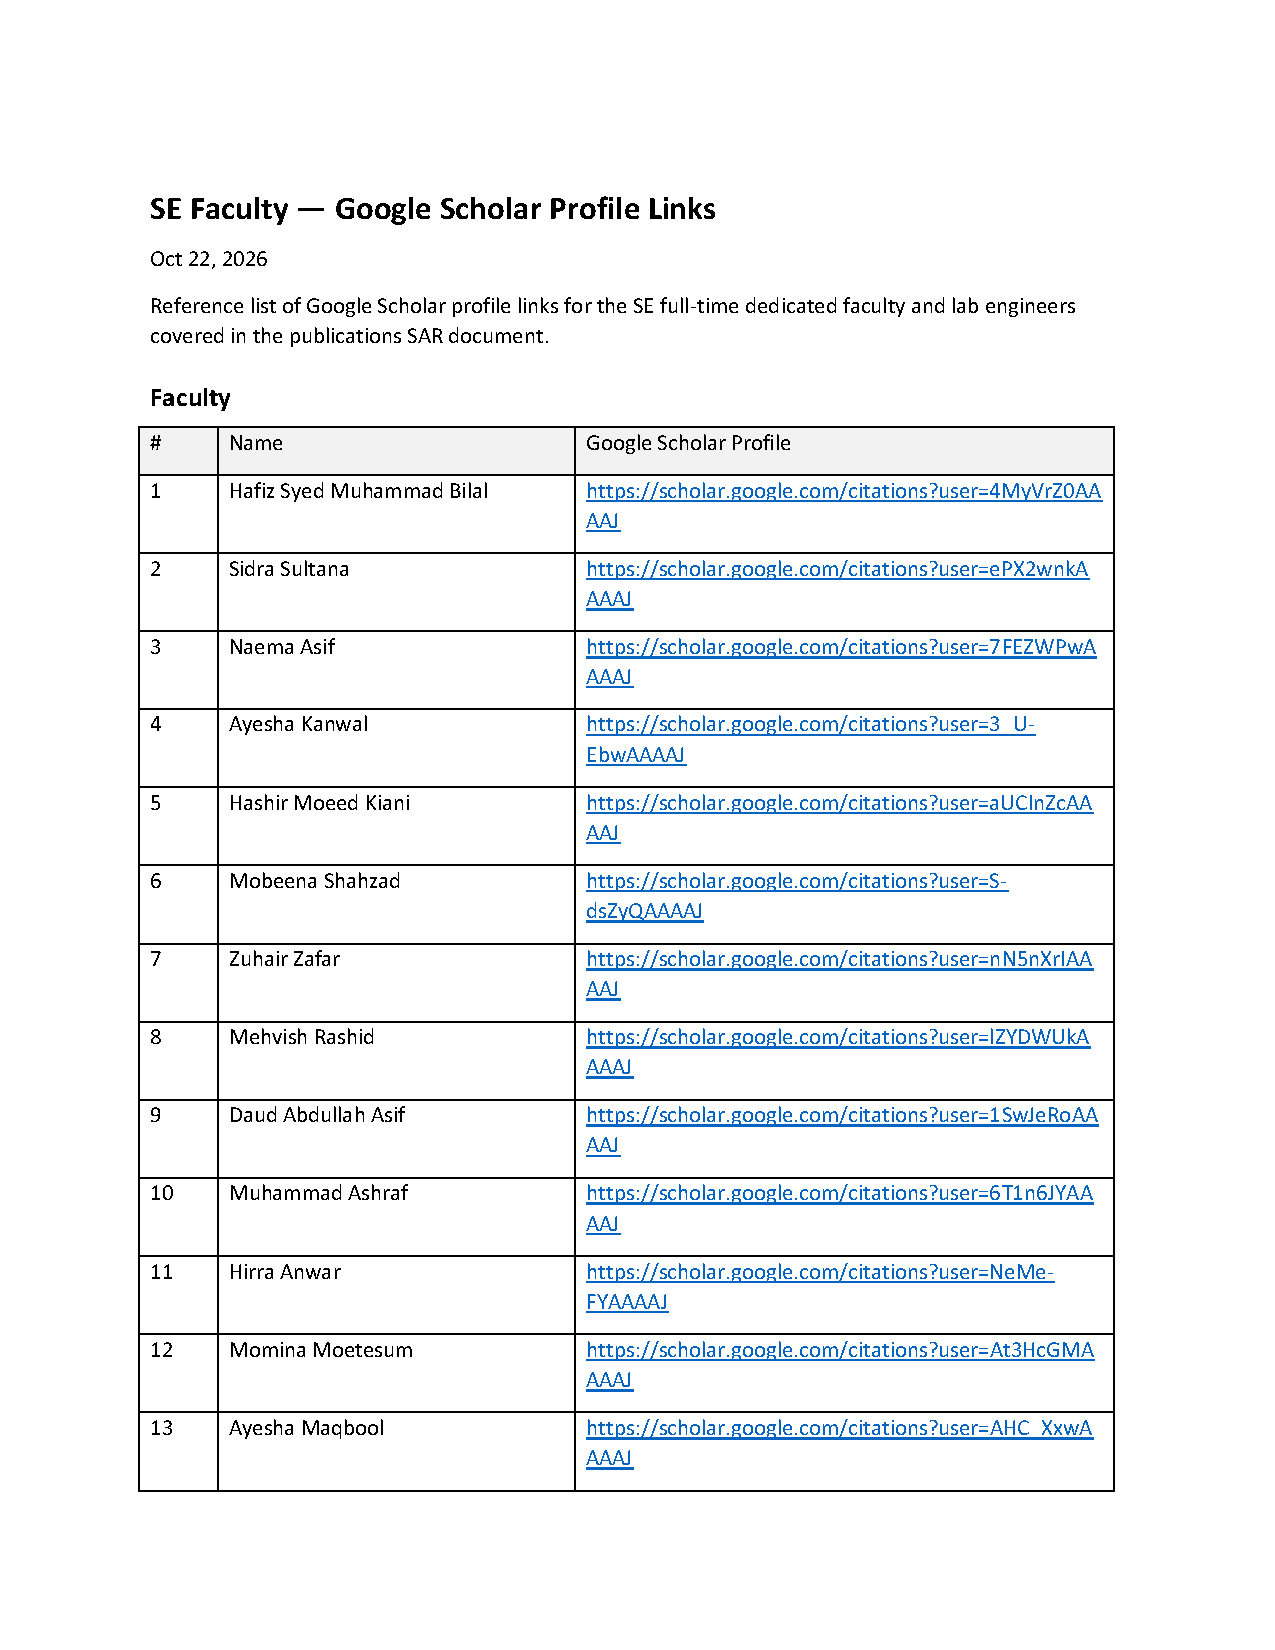
\includepdf[
  pages={1},
  scale=0.90,
  offset=0 -1.2cm,
  pagecommand={\thispagestyle{plain}\noindent{\Large\bfseries\thesection\quad Google Scholar Profiles of FTDF of SE}}
]{appendices/criterion_5/research-data.pdf}

%\refstepcounter{section}
%\phantomsection
%\label{annex:AH}
%\addcontentsline{toc}{section}{\protect\numberline{\thesection}Service Gratuity Programme Details}
%
\includepdf[
%  pages={-},
%  scale=0.90,
%  offset=0 -2.2cm,
%  pagecommand={\thispagestyle{plain}\noindent{\Large\bfseries\thesection\quad Service Gratuity Programme Details}}
%]{appendices/criterion_5/Annex E2.pdf}







\clearpage
\clearpage
\setcounter{section}{0}
\renewcommand{\thesection}{F.\arabic{section}}
\renewcommand{\theHsection}{annexF.\arabic{section}}

\phantomsection
\addcontentsline{toc}{chapter}{Annexure F: Criteria 6 Supporting Documents}
\label{app:criteria-6}

\refstepcounter{section}
\phantomsection
\label{annex:labs_labwork}
\addcontentsline{toc}{section}{\protect\numberline{\thesection}Laboratories and Lab Work}

% ---- Heading block defined as a (long) macro, so \par is allowed ----
\newcommand{\annexFFirstPageHead}{%
  \noindent{\Huge\bfseries Annexure F: Criteria 6 Supporting Documents}\par
  \vspace{0.8em}
  \noindent Here we provide the supporting annexures required for Criterion 6: Facilities and Infrastructure.\par
  \vspace{0.8em}
  \noindent{\Large\bfseries\thesection\quad 
  Laboratories and Lab Work}\par
}

% ---- Page 1: heading + shrunk PDF page ----
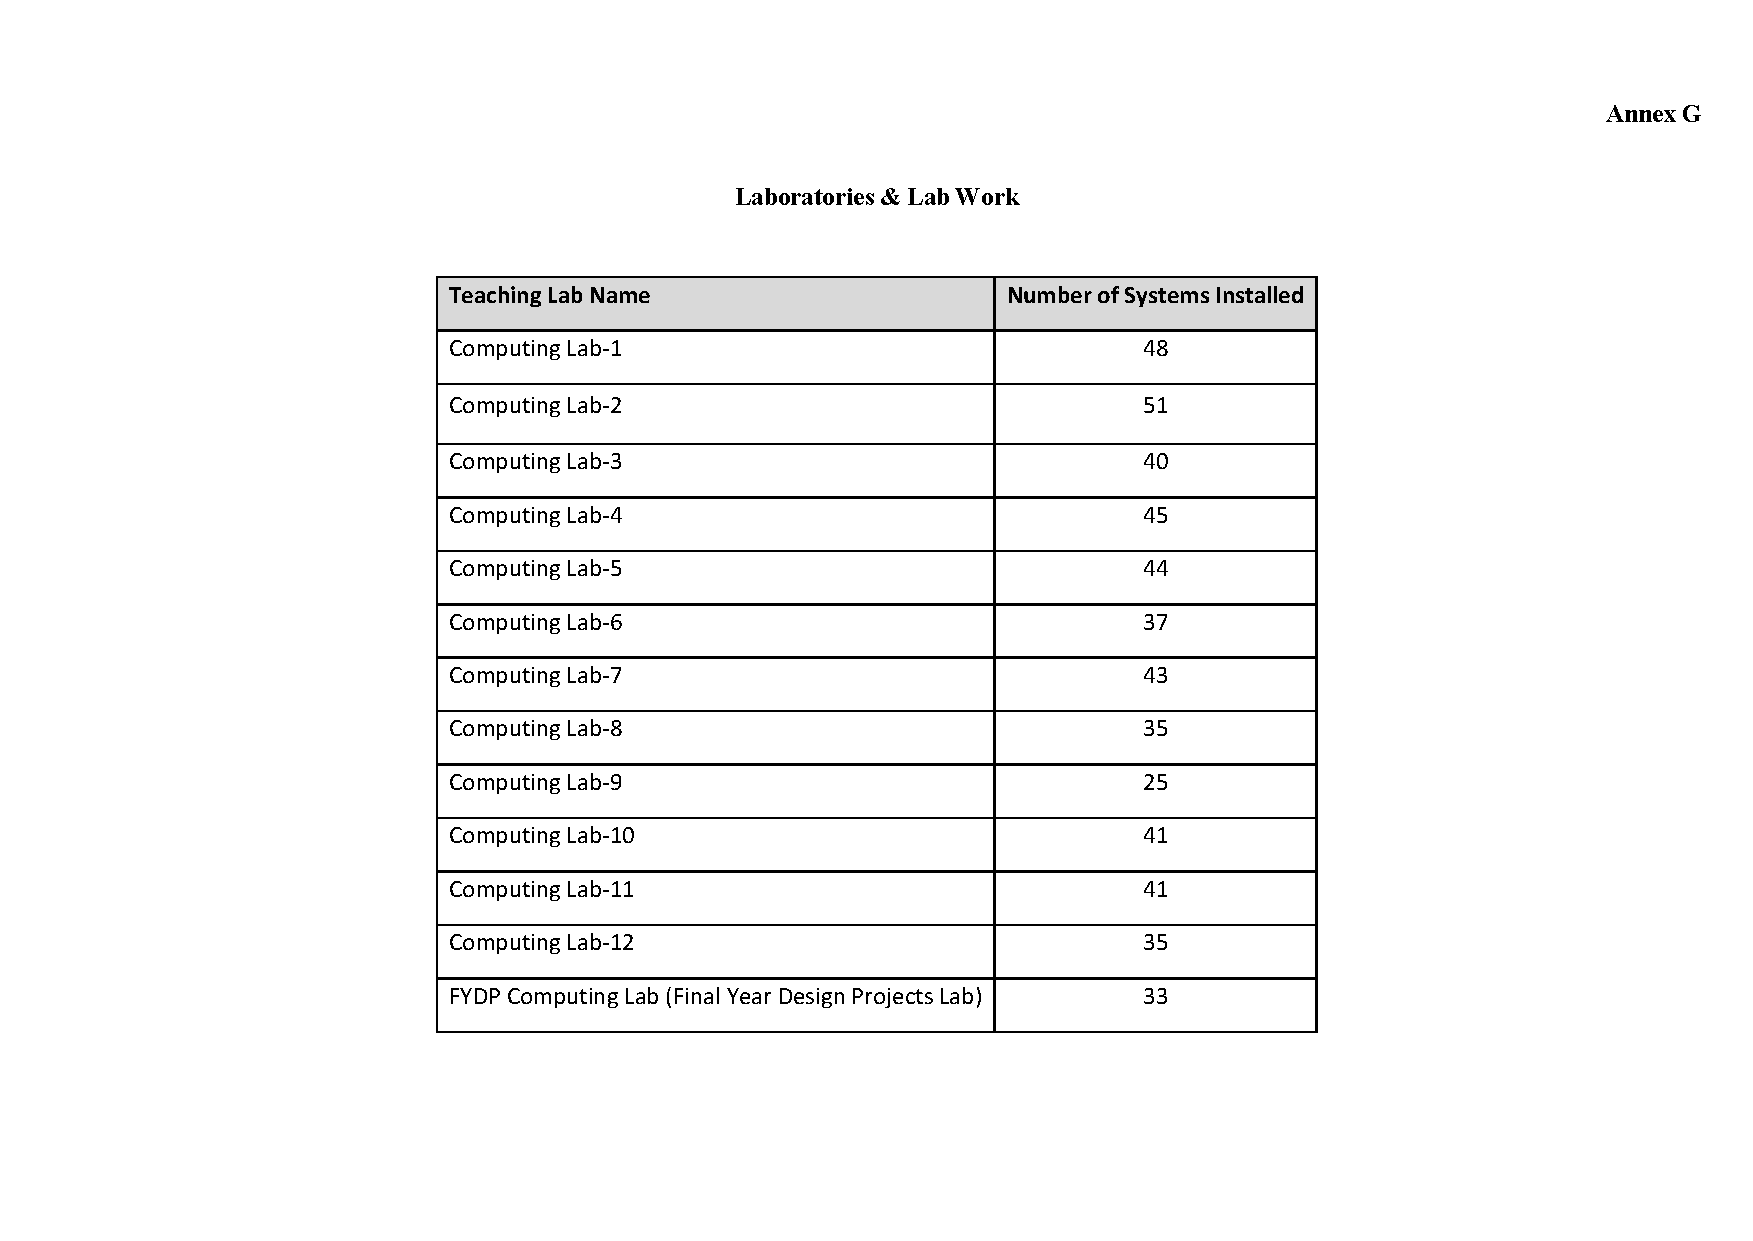
\includepdf[
  pages={1},
  scale=0.95,
  landscape,
  offset=0 -0.2cm,
  pagecommand={\thispagestyle{plain}\annexFFirstPageHead}
]{appendices/criterion_6/Lab_data.pdf}

% ---- Pages 2 to end: unchanged ----
\includepdf[
  pages={2-},
  landscape,
  pagecommand={\thispagestyle{plain}}
]{appendices/criterion_6/Lab_data.pdf}


%\includefullannexure{appendices/criterion_6/Laboratories_and_Labwork.pdf}

\refstepcounter{section}
\phantomsection
\label{annex:NUST healthsafetypolicy}
\addcontentsline{toc}{section}{\protect\numberline{\thesection}NUST Health, Safety and Envrionment Policy}

\includepdf[
  pages={1},
  scale=0.90,
  offset=0 -1.2cm,
  pagecommand={\thispagestyle{plain}\noindent{\Large\bfseries\thesection\quad NUST Health, Safety and Envrionment Policy}}
]{appendices/criterion_6/health.pdf}


\includepdf[
  pages={2-},
  pagecommand={\thispagestyle{plain}}
]{appendices/criterion_6/health.pdf}

%\section{NUST Health, Safety and Envrionment Policy}
%\label{annex:NUST healthsafetypolicy}
%\includefullannexure{appendices/criterion_6/University_health_safety_and_environment_policy.pdf}

\refstepcounter{section}
\phantomsection
\label{annex:work health safety checklist}
\addcontentsline{toc}{section}{\protect\numberline{\thesection}Work, Health and Safety Induction Checklist}
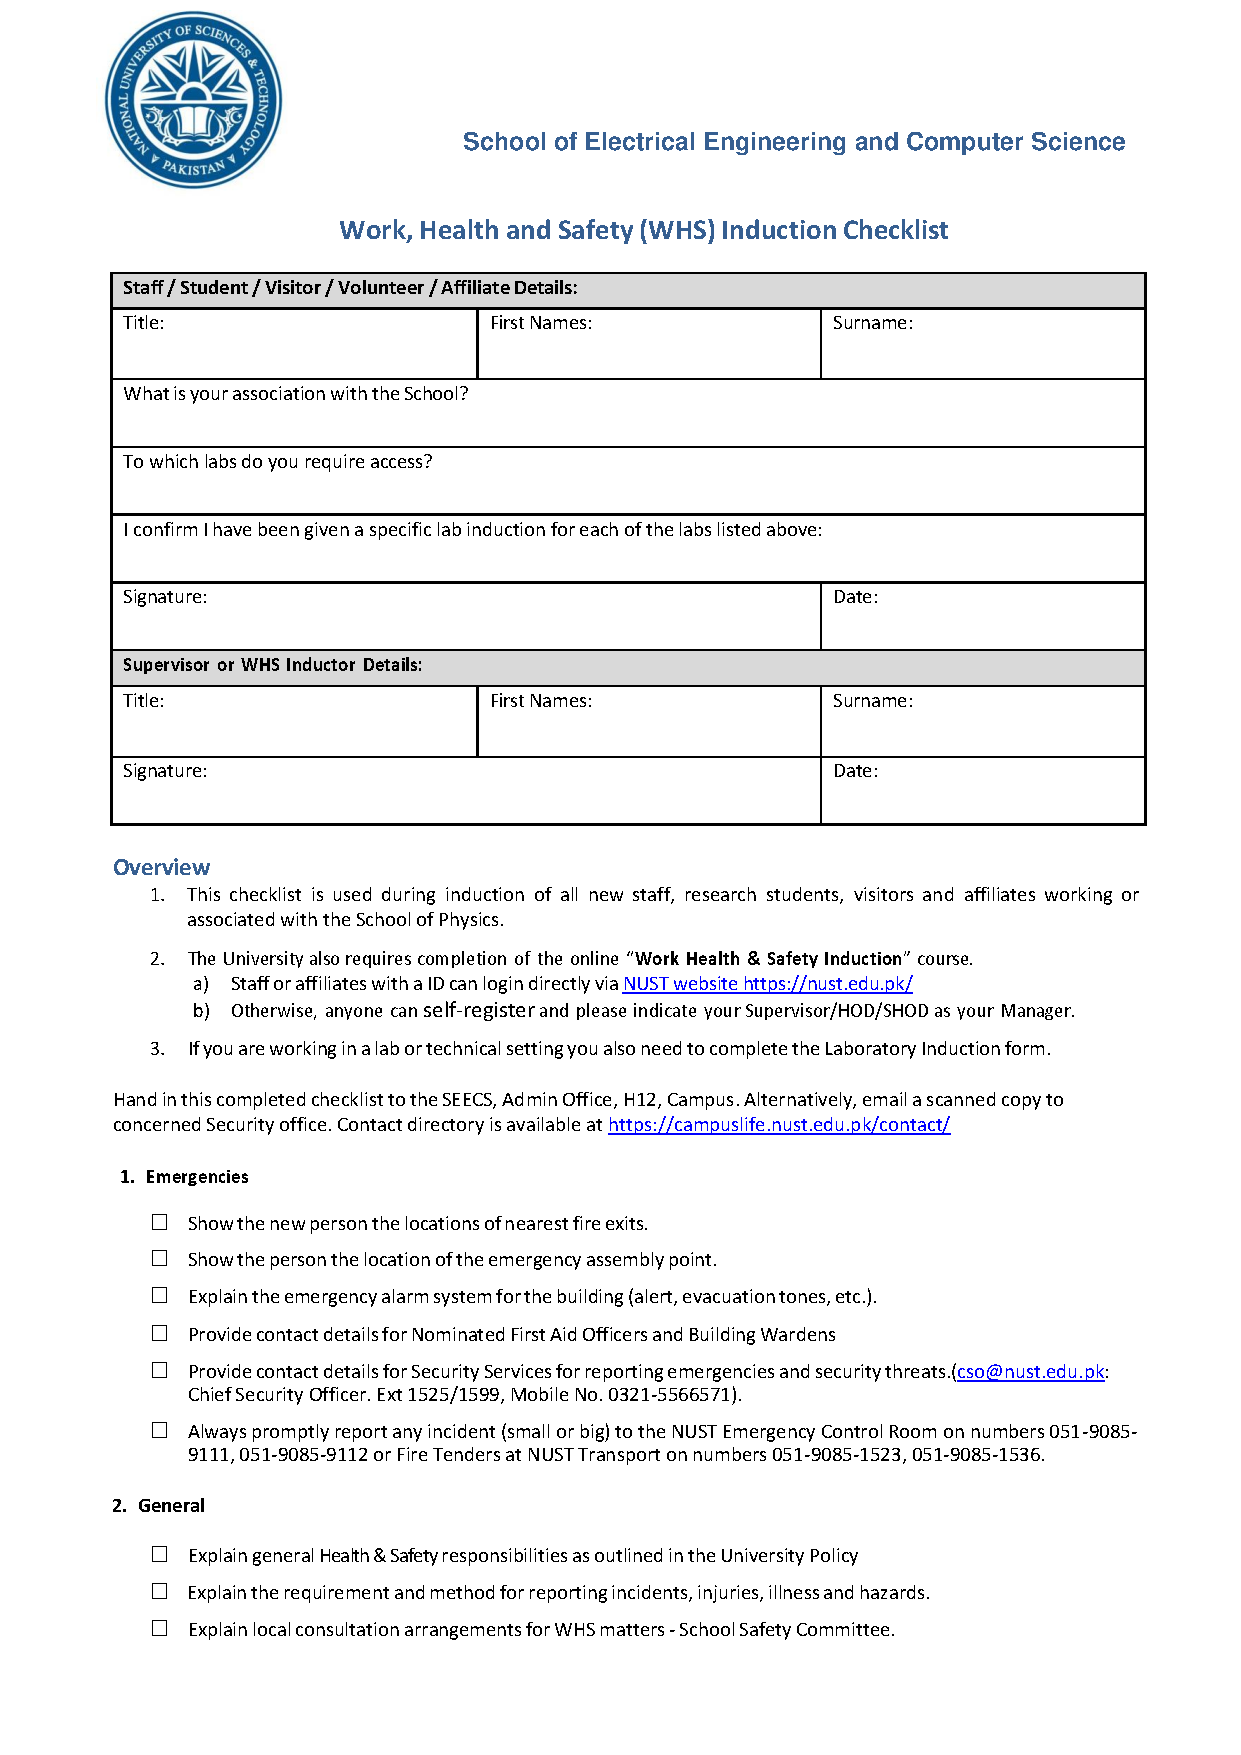
\includepdf[
  pages={1},
  scale=0.90,
  offset=0 -2.2cm,
  pagecommand={\thispagestyle{plain}\noindent{\Large\bfseries\thesection\quad Work, Health and Safety Induction Checklist}}
]{appendices/criterion_6/Work_health_and_safety_induction_checklist.pdf}

\includepdf[
  pages={2-},
  pagecommand={\thispagestyle{plain}}
]{appendices/criterion_6/Work_health_and_safety_induction_checklist.pdf}









\clearpage
\clearpage
\setcounter{section}{0}
\renewcommand{\thesection}{G.\arabic{section}}
\renewcommand{\theHsection}{annexG.\arabic{section}}

\chapter*{Annexure G: Criteria 7 Supporting Documents}
\phantomsection
\addcontentsline{toc}{chapter}{Annexure G: Criteria 7 Supporting Documents}
\label{app:criteria-7}
% ------------------------------------------------------------
\section{Detailed Financial Data}
\label{annex:L}

\noindent
Detailed breakdown of scholarship support, income, research funding, and budgeted versus
actual expenditures for SEECS during the accreditation cycle (2022--23 to 2025--26).

\begin{table}[H]
\centering
\caption{Annex L: Scholarship Financial Support, SEECS (Rupees in Million).}
\label{tab:annexL_scholarships}
\begingroup\small
\begin{tabular}{>{\raggedright\arraybackslash}p{0.32\textwidth}rrrr>{\raggedright\arraybackslash}p{0.20\textwidth}}
\toprule
\textbf{Account Head} & \textbf{2022--23} & \textbf{2023--24} & \textbf{2024--25} & \textbf{2025--26} & \textbf{Remarks} \\
\midrule
Board Scholarships & 1.508 & 1.470 & 0.655 & 0.198 & Upto 30 June 2026 \\
GPA Based Financial Assistances & 3.492 & 3.450 & 3.687 & 3.975 & Upto 30 June 2026 \\
HEC Scholarships & 1.109 & 6.666 & 1.608 & 7.813 & Upto 30 June 2026 \\
MS leading to PhD Students Scholarships & 1.164 & 4.217 & 2.534 & 0.239 & Upto 30 June 2026 \\
Need based Scholarships & 20.524 & 1.986 & 5.859 & 0.303 & Upto 30 June 2026 \\
\bottomrule
\end{tabular}
\endgroup
\end{table}

\begin{table}[H]
\centering
\caption{Annex L: Income and Research Funding, SEECS (Rupees in Million).}
\label{tab:annexL_income}
\begingroup\small
\begin{tabular}{>{\raggedright\arraybackslash}p{0.36\textwidth}rrrr>{\raggedright\arraybackslash}p{0.24\textwidth}}
\toprule
\textbf{Account Head} & \textbf{2022--23} & \textbf{2023--24} & \textbf{2024--25} & \textbf{2025--26} & \textbf{Remarks} \\
\midrule
Research Project Funding & 46.583 & 70.217 & 73.262 & 69.940 & Actual upto 30 June 2026 \\
Student Tuition Fee (Self-Funded) & 594.764 & 753.222 & 889.700 & 1107.514 & Actual Fall 2025 and Spring 2026 \\
\bottomrule
\end{tabular}
\endgroup
\end{table}

% Landscape table — requires \usepackage{pdflscape}
\begin{landscape}
\begin{longtable}{p{4.4cm}rrrrrrrrp{3.2cm}}
\caption{Annex L: Budgeted and Actual Expenses, SEECS (Rupees in Million).}\label{tab:annexL_expenses}\\
\toprule
\textbf{Account Head} & \multicolumn{2}{c}{\textbf{2022--23}} & \multicolumn{2}{c}{\textbf{2023--24}} & \multicolumn{2}{c}{\textbf{2024--25}} & \multicolumn{2}{c}{\textbf{2025--26}} & \textbf{Remarks} \\
\cmidrule(lr){2-3}\cmidrule(lr){4-5}\cmidrule(lr){6-7}\cmidrule(lr){8-9}
& \textbf{Budgeted} & \textbf{Actual} & \textbf{Budgeted} & \textbf{Actual} & \textbf{Budgeted} & \textbf{Actual} & \textbf{Budgeted} & \textbf{Actual} & \\
\midrule
\endfirsthead
\toprule
\textbf{Account Head} & \multicolumn{2}{c}{\textbf{2022--23}} & \multicolumn{2}{c}{\textbf{2023--24}} & \multicolumn{2}{c}{\textbf{2024--25}} & \multicolumn{2}{c}{\textbf{2025--26}} & \textbf{Remarks} \\
\cmidrule(lr){2-3}\cmidrule(lr){4-5}\cmidrule(lr){6-7}\cmidrule(lr){8-9}
& \textbf{Budgeted} & \textbf{Actual} & \textbf{Budgeted} & \textbf{Actual} & \textbf{Budgeted} & \textbf{Actual} & \textbf{Budgeted} & \textbf{Actual} & \\
\midrule
\endhead
Faculty and Support Staff salaries & 461.508 & 461.508 & 477.152 & 477.152 & 580.086 & 580.086 & 632.311 & 632.311 & Actual upto 30 June 2026 \\
Lab Equipment & 10.000 & 10.000 & 8.400 & 8.400 & 71.550 & 71.550 & 75.230 & 74.820 & Actual upto 30 June 2026 \\
Software Purchase & 4.700 & 4.700 & 6.700 & 6.700 & 10.400 & 10.400 & 0.000 & 0.000 & -- \\
Lab Consumables & 0.900 & 0.900 & 0.800 & 0.800 & 0.600 & 0.600 & 0.700 & 0.700 & Actual upto 30 June 2026 \\
Maintenance of existing facilities & 19.700 & 19.700 & 23.887 & 23.887 & 35.700 & 35.700 & 74.609 & 74.601 & Actual upto 30 June 2026 \\
Repair \& Maintenance & 1.000 & 1.000 & 2.140 & 2.140 & 1.000 & 1.000 & 0.500 & 0.500 & Actual upto 30 June 2026 \\
Other Misc. Expenses & 3.300 & 3.300 & 5.000 & 5.000 & 5.000 & 5.000 & 33.940 & 23.270 & Actual upto 30 June 2026 \\
\bottomrule
\end{longtable}
\end{landscape}

\clearpage
\clearpage
\setcounter{section}{0}
\renewcommand{\thesection}{H.\arabic{section}}
\renewcommand{\theHsection}{annexH.\arabic{section}}

\phantomsection
\addcontentsline{toc}{chapter}{Annexure H: Criteria 8 Supporting Documents}
\label{app:criteria-8}

\refstepcounter{section}
\phantomsection
\label{app:cqi}
\addcontentsline{toc}{section}{\protect\numberline{\thesection}Rejoinder}

% ---- Heading block ----
\newcommand{\annexHFirstPageHead}{%
  \noindent{\Huge\bfseries Annexure H: Criteria 8 Supporting Documents}\par
  \vspace{0.8em}
  \noindent Here we provide the supporting annexures required for Criterion 8: Continuous Quality Improvement (CQI).\par
  \vspace{0.8em}
  \noindent{\Large\bfseries\thesection\quad Rejoinder}\par
  \vspace{0.5em}
}

% Display the heading before the table
\annexHFirstPageHead
This rejoinder presents the responses and clarifications provided by the Software Engineering Department at SEECS to the observations and recommendations arising from the previous accreditation review under Criterion 8: Continuous Quality Improvement (CQI). It summarizes the actions taken to address the identified issues, the improvements implemented, and the measures adopted to strengthen continuous quality improvement practices within the programme. The rejoinder is supported by relevant documentary evidence, presented in the following table, to facilitate verification of the responses and the progress achieved.
\begin{landscape}
\label{annex:rejoinder}
\scriptsize

\begin{longtable}{|P{2.3cm}|P{5.0cm}|P{4.5cm}|P{5.0cm}|P{2.4cm}|P{2.8cm}|P{1.8cm}|}
\hline
\rowcolor{gray!25}
\textbf{Criteria} & \textbf{PEC Observation} & \textbf{Root Cause Analysis} & \textbf{Corrective Action Plan} & \textbf{Implementation Status} & \textbf{Evidence} & \textbf{Reference to SAR} \\
\hline
\endfirsthead
\hline
\rowcolor{gray!25}
\textbf{Criteria} & \textbf{PEC Observation} & \textbf{Root Cause Analysis} & \textbf{Corrective Action Plan} & \textbf{Implementation Status} & \textbf{Evidence} & \textbf{Reference to SAR} \\
\hline
\endhead

\multirow{2}{=}{\textbf{PEO}} & The process for assessing the achievement of Program Educational Objectives (PEOs) is clear. Key Performance Indicators (KPIs) are well-defined, and assessment tools are in use. However, there is a noticeable lack of correlation in the survey forms used to assess certain sub-KPIs related to PEO-2 and PEO-3. The cumulative KPI attainment process is well-documented in the approved policy. & The observation regarding the lack of correlation between certain survey items and the sub-KPIs of PEO-2 and PEO-3 is acknowledged. On review of the existing alumni and employer survey forms, the Department confirmed this concern and further noted that some questions were vaguely framed and that the PEOs were assessed through an uneven number of questions. & The Department undertook a review activity and comprehensively revised both the alumni and employer survey forms. In the revised questionnaires, each question is directly aligned to a specific PEO, ambiguity has been removed, and every PEO is now measured through an equal number of questions to ensure balanced and valid attainment. & Complete & Alumni \& Employer Survey Forms & Sec.~\ref{revised-assesment-instrument}; Annex~\ref{app:revised forms}, \ref{annex:alumni}, \ref{annex:employer} \\ \hline
 & The Continuous Quality Improvement (CQI) process at the Program Educational Objectives (PEO) level has been initiated. Some assessment data has been collected using existing survey forms, and analysis and evaluation have been conducted. Stakeholder feedback is also gathered for the revision of survey forms. Corrective actions have been identified, but there are issues with the implementation of these actions. & Although PEO assessment data and stakeholder feedback were being collected, the Department lacked a structured mechanism to systematically implement, monitor, and document corrective actions arising from the evaluation results. In addition, the PEO assessment methodology and survey instruments required further refinement to support effective CQI implementation. & Comprehensively revise the stakeholder survey instruments, improve the PEO KPI evaluation mechanism through a structured assessment methodology, and incorporate Industrial Advisory Board feedback to strengthen the PEO assessment and review process. & Complete & IAB Meeting Minutes, Evaluation System mentioned in Criteria 1 & Sec.~\ref{attainment-of-peos}, \ref{attainment-results}, \ref{program-improvement}, \ref{subsec:new-peo-evaluation-framework}; Annex~\ref{app:iab_feedback_full}, \ref{app:iab_minutes} \\ \hline
\multirow{4}{=}{\textbf{PLO}} & The department has updated the Program Educational Outcomes (PEOs), but it appears that some essential elements of PEO-2 are not addressed in the Program Learning Outcomes (PLOs). & During the review of the PEO–PLO alignment, it was identified that the mapping did not explicitly capture the "innovative solution development" component of PEO-2. Although PLO-8, PLO-9, and PLO-10 addressed leadership, teamwork, communication, and project management, the design and innovation aspect was omitted from the mapping. & The PEO–PLO mapping was reviewed and revised to explicitly align PEO-2 with PLO-3 (Design/Development of Solutions) in addition to PLO-8, PLO-9, and PLO-10. The updated mapping ensures comprehensive coverage of leadership, teamwork, communication, project management, and innovative solution development within PEO-2. & Complete & Updated Mapping available in Crteria 2 of SAR & Sec.~\ref{sec:plopeo}; Annex~\ref{app:criteria-2_plo-peo_mapping_rationale} \\ \hline
 & The course-to-PLO mapping demonstrates satisfactory alignment with all PLOs. Nevertheless, there are notable weaknesses in the mapping, particularly concerning PLO-3 and PLO-1, in terms of the learning domain and taxonomy level. However, the department has provided data regarding the ongoing mapping revision for upcoming semesters, which is based on Continuous Quality Improvement (CQI) and utilizes the course review performa. & The review identified that the CLOs of certain courses were not optimally aligned with the intended learning domains and Bloom's Taxonomy levels of PLO-1 and PLO-3. As a result, the course-to-PLO mapping did not fully reflect the required cognitive complexity and expected outcome attainment. & Implemented a comprehensive review and revision of course specifications, including refinement of CLOs, updating Bloom's Taxonomy levels and learning domains, and revising the course-to-PLO mapping through the departmental CQI process based on Course Review Reports, faculty discussions, and DBS recommendations. & Completed & CLO-PLO Mapping available in Criteria 2 & Sec.~\ref{sec:cloplo}; Annex~\ref{OBE Assessment Configuration on Qalam} \\ \hline
 & Assessment methodologies, including both direct and indirect methods, are established. However, the assessment methods for achieving PLOs through indirect means need improvement, especially in the case of the poorly designed internship form and the graduate exit survey forms. Furthermore, although direct assessment methods are in use, they are not consistently applied in certain instances for a couple of PLOs, specifically PLO-8 and PLO-10. & The review identified that the Internship Employer Feedback Form and Graduate Exit Survey Form were not adequately aligned with the Program Learning Outcomes and lacked well-defined assessment indicators for reliable indirect assessment. In addition, direct assessment of PLO-8 and PLO-10 was not consistently integrated into the CLOs and assessment instruments of relevant courses. & The Internship Employer Feedback Form and Graduate Exit Survey Form were comprehensively revised to improve clarity, incorporate well-defined PLO-based assessment indicators, and strengthen indirect assessment. An online Internship Feedback Module was integrated with the Thesis Management System (TMS) to institutionalize employer feedback collection and reporting. Additionally, the direct assessment methodology was reviewed and updated by revising CLO-to-PLO mappings and course specifications to ensure consistent assessment of all PLOs, including PLO-8 and PLO-10, through appropriate assessment instruments. & Complete & Internship Feedback Form \& Graduate Exit Survey Form and CLO-PLO Mapping & Sec.~\ref{sec:indirectassess}, \ref{revised-assesment-instrument}, \ref{subsec:new-internship-mechanism}, \ref{sec:cloplo}; Annex~\ref{annex:internship-feedback-form}, \ref{annex:internship-feedback-analysis}, \ref{annex:graduate-exit-survey-form}, \ref{annex:graduate-exit-survey-analysis} \\ \hline
 & The Key Performance Indicators (KPIs) are clearly defined. However, there is an issue with the assessment process in direct assessment, as it is not consistently conducted at the appropriate taxonomy level. Additionally, the quality of the assessment process in the case of indirect methods appears to be subpar, especially when using the internship feedback form. & The review identified that the assessment instruments of some courses were not consistently aligned with the intended Bloom's Taxonomy levels defined for the CLOs, resulting in inconsistencies in direct assessment. Additionally, the existing Internship Employer Feedback Form lacked well-defined PLO-based assessment indicators and a structured mechanism for systematic data collection and analysis, reducing the effectiveness of indirect assessment. & Conducted a comprehensive review and revision of course specifications, including CLOs, Bloom's Taxonomy levels, and assessment instruments, to ensure direct assessment is performed at the intended cognitive level and aligned with the relevant PLOs. The Internship Employer Feedback Form was comprehensively redesigned with improved PLO-based assessment indicators, and an Online Internship Feedback Module integrated with the Thesis Management System (TMS) was implemented to institutionalize employer feedback collection, reporting, and analysis, thereby improving the reliability, consistency, and traceability of indirect assessment data. & Indirect assesment method Complete, Continuously improving mappings through CQI Cycles & Internship Feedback Form, Course Outlines for Information Security \& Software Design \& Architecture & Sec.~\ref{revised-assesment-instrument}, \ref{subsec:new-internship-mechanism}, \ref{sec:cloplo}; Annex~\ref{annex:internship-feedback-form} \\ \hline
\multirow{5}{=}{\textbf{Curriculum}} & The department has supplied a list of courses that cover CEP attributes. The visitation team has been presented with data related to CEPs and their assessments. However, the visitation team has observed a lack of understanding in the assessment of CEPs, along with identified weaknesses concerning the clarity and complexity level of CEP attributes in statements provided, particularly in a few courses. & The review identified that faculty members had varying levels of understanding regarding the formulation, mapping, and assessment of Complex Engineering Problem (CEP) attributes. In addition, the absence of standardized guidelines resulted in inconsistencies in the clarity and cognitive complexity of CEP statements across a few courses. & Conducted dedicated faculty training sessions on the formulation, mapping, and assessment of CEP attributes in accordance with PEC guidelines. A standardized CEP template, along with illustrative examples, was developed and disseminated to all course instructors to ensure consistent formulation, appropriate complexity levels, and uniform assessment of CEP attributes across courses. & Complete & CEP Training List, CEP Guidelines & Sec.~\ref{sec:4.2cep}, \ref{subsubsec:cep-oel}; Annex~\ref{app:criteria-3_CEP Policy for BESE Department}, \ref{app:criteria-3_CEP Example} \\ \hline
 & The use of rubrics-based assessment mechanisms in the lab is evident, as observed from the lab folders and during the visit to the labs. However, it is noted that the assessment mechanisms, especially in the Psychomotor and Affective domains, are not appropriate in certain lab courses, such as operating systems and deep learning. The visitation team also observed inconsistencies in the experiments included in the lab folders of a few courses, like Computer Architecture and Logic Design, where the experiments did not align with the course contents as per the syllabus. & The department's Continuous Quality Improvement review identified opportunities to further refine laboratory assessment practices and standardize laboratory content to ensure consistent alignment with the approved course syllabi, intended learning outcomes, and Bloom's Taxonomy levels. & Conducted dedicated training sessions for faculty members and lab engineers on the design of open-ended lab exercises and rubric-based assessment of the Psychomotor and Affective domains. In addition, a standardized laboratory manual template was developed and implemented across the Software Engineering Department to ensure consistency in laboratory content, alignment with approved course outlines, and uniform assessment practices. The laboratory assessment rubrics and manuals were also reviewed to ensure appropriate alignment with the intended learning outcomes and Bloom's Taxonomy levels. & Complete & OEL Training, Standardized Template, Rubrics Sample & Sec.~\ref{sec:labrubrics}, \ref{sec:labassessment}, \ref{subsubsec:cep-oel}; Annex~\ref{app:criteria-3_Sample Lab Manual}, \ref{app:criteria-3_Lab Rubric Based Evaluation}, \ref{app:criteria-3_Sample Open Ended Lab} \\ \hline
 & Course Learning Outcomes (CLOs) are defined for all courses, but the visitation team has identified issues with the taxonomy levels and their mapping to relevant Program Learning Outcomes (PLOs) in many course outlines. This discrepancy is notably observed in courses like Design and Analysis of Algorithms and Operating Systems etc. & The department's periodic review of course specifications identified opportunities to further refine the formulation of Course Learning Outcomes (CLOs) and strengthen their alignment with the intended Bloom's Taxonomy levels, learning domains, and corresponding Program Learning Outcomes (PLOs) in a few courses. & Conducted a comprehensive review and revision of course specifications through the departmental CQI process. Course Learning Outcomes were refined to improve clarity and measurability, Bloom's Taxonomy levels and learning domains were updated where required, and course-to-PLO mappings were revised based on Course Review Reports, faculty deliberations, and Departmental Board of Studies (DBS) recommendations. The revised course specifications have been implemented in the current curriculum to ensure appropriate cognitive complexity and improved alignment with the intended PLOs. & Complete & CLO-PLO Mapping available in Criteria 2 & Sec.~\ref{sec:cloplo}, \ref{sec:4.10assessment}; Annex~\ref{app:criteria-3_Course Outline with Knowledge Group Head's Signature} \\ \hline
 & Assessment in the knowledge domain is generally appropriate, but at times it lacks rigor, as evident from the course folders, particularly in courses like Operating System, Organizational Behavior, and Computer Architecture and Logic Design. The assessments in the Psychomotor and Affective domains also require significant improvement for the evaluation of Course Learning Outcomes (CLOs) and Program Learning Outcomes (PLOs). Additionally, it was noted that rubrics are not consistently followed for assessment in the Affective domain in some courses, specifically those mapped to PLO-10. & The department's periodic review identified opportunities to further enhance the consistency and rigor of assessment instruments across a few courses, particularly in strengthening the evaluation of the Psychomotor and Affective domains and ensuring the uniform application of rubric-based assessment for courses mapped to PLO-10. & Conducted dedicated Outcome-Based Education (OBE) training sessions for faculty members of the Humanities and Sciences Department, who primarily offer courses mapped to PLO-8 and PLO-10, to strengthen their understanding of rubric-based assessment, appropriate CLO coverage, and alignment with Bloom's Taxonomy levels. Faculty members were also instructed to develop and include assessment rubrics for every Psychomotor and Affective domain assessment to ensure consistent, transparent, and outcome-based evaluation. These initiatives have enhanced the quality, consistency, and rigor of assessment practices across the relevant courses. & Complete & H\&S Training Minutes \& Feedback, Rubrics Sample for Affective Domain & Sec.~\ref{sec:labrubrics}, \ref{subsec:faculty-development-training}, \ref{criterion-8-review-and-corrective-action-processes-for-clos}; Annex~\ref{app:criteria-3_Lab Rubric Based Evaluation} \\ \hline
 & Satisfactory attainment is observed in all three domains. However, the visitation team noted that in several courses (e.g., Design and Analysis of Algorithms, Software Design and Architecture, Formal Methods, Internet of Things, etc.), assessments for Course Learning Outcomes (CLOs) are conducted at a lower taxonomy level. This should be addressed through Continuous Quality Improvement (CQI). It is also worth mentioning that despite the lower taxonomy levels, the assessment appears to be at a suitable level of complexity, indicating a potential lack of faculty understanding about taxonomy levels. This is an area that requires improvement. & The department's periodic review identified opportunities to further strengthen the consistency between the documented Bloom's Taxonomy levels of certain Course Learning Outcomes (CLOs) and the cognitive complexity of the corresponding assessment instruments. The review also highlighted the need for greater consistency in the application of Bloom's Taxonomy during course design and assessment planning. & Conducted a comprehensive review of the affected course specifications through the departmental CQI process and revised the Course Learning Outcomes (CLOs), Bloom's Taxonomy levels, and course-to-PLO mappings to accurately reflect the intended cognitive complexity of the assessments. Faculty awareness of Bloom's Taxonomy was further strengthened through curriculum review meetings and internal OBE discussions to promote the consistent application of taxonomy levels during course design, assessment planning, and periodic course reviews. & Complete & CLO-PLO Mappin, CQI cycle for CLO revision samples & Sec.~\ref{sec:cloplo}, \ref{sec:cqiclos}, \ref{criterion-8-review-and-corrective-action-processes-for-clos}; Annex~\ref{annex:caf-oop}, \ref{annex:dbs-mom}, \ref{annex:oop} \\ \hline
\multirow{2}{=}{\textbf{Faculty \& Support Staff}} & There is a formal training mechanism in place for faculty development; however, it has been noted that this mechanism does not comprehensively cover all areas, particularly those related to learning domains and taxonomy levels. & The department's review identified an opportunity to further strengthen and formalize faculty development activities related to Outcome-Based Education (OBE), particularly in the consistent application of learning domains, Bloom's Taxonomy levels, and constructive alignment during course design and assessment. & Strengthened the departmental faculty development mechanism by institutionalizing dedicated OBE training for newly inducted faculty through the NNUST Certificate for Teaching \& Learning (NCTL) and conducting regular refresher workshops at the department and SEECS levels. The training covers the formulation of measurable CLOs, selection of appropriate learning domains and Bloom's Taxonomy levels, CLO–PLO mapping, design of aligned assessment instruments, and constructive alignment of teaching, learning, and assessment. Faculty participation in national and international professional development programs has also been encouraged to further enhance pedagogical and technical competencies. & Repeated at Regular Intervals & Training List & Sec.~\ref{sec:training}, \ref{subsec:faculty-development-training} \\ \hline
 & Most of the teaching staff in the department are in the early stages of their academic careers, with a significant number being junior faculty members. & The department's faculty expansion in recent years has included the recruitment of talented early-career academics to support program growth and future capacity building. To ensure consistency in academic quality and Outcome-Based Education (OBE) practices, structured mentoring and professional development were identified as key enablers for faculty development. & Maintained a balanced faculty profile in which more than 60\% of the faculty members possess around 10 years or more of academic and/or industry experience, providing strong academic leadership and mentoring. Strengthened the faculty development framework by implementing structured induction and mentoring programs for newly inducted faculty, including mandatory OBE training through the NUST Certificate for Teaching \& Learning (NCTL), supervised teaching, and continuous professional development activities. Junior faculty members were paired with experienced mentors to support curriculum delivery, assessment practices, research supervision, and adherence to departmental quality assurance processes, ensuring continuity and sustained academic excellence. & Repeated at Regular Intervals & Faculty List available in Chapter 5 & Sec.~\ref{faculty-strength-and-competencies}, \ref{sec:training}; Annex~\ref{annex:I}, \ref{annex:J} \\ \hline
\multirow{1}{=}{\textbf{Facilities and Infrastructure}} & The library has successfully acquired a substantial collection of books; however, it is currently facing budget-related constraints that need to be addressed in order to accommodate future growth. In addition to traditional resources, digital library resources are also available. It's worth noting that the library software is accessible, offering the potential for efficient resource management and organization once access issues are resolved. Efforts to expand physical space, address system-related challenges, and optimize the library software will greatly enhance the overall library experience for students and faculty, enabling seamless access to a wide range of educational resources. & The NUST Library System provides a comprehensive collection of print and digital resources supported by established library management processes and periodic institutional reviews. As part of its continuous enhancement approach, these reviews identified opportunities to further optimize library services, digital resource accessibility, library management systems, and learning spaces to better support the evolving academic and research requirements of students and faculty. & Strengthened library services through continuous enhancement of the Central Library facilities, regular maintenance and upgrading of the KOHA Integrated Library Management System and DSpace Institutional Repository, and ongoing coordination with the ICT Directorate to improve network reliability and access to electronic resources. Expanded access to national and international digital resources, including the HEC Digital Library and major scholarly databases, while continuously updating the Institutional Repository with research publications and theses. Future enhancement initiatives have also been planned, including expansion of seating capacity, improved collaborative learning spaces, dedicated research commons, and AI-enabled library support services. & In-Process &  & Sec.~\ref{library}, \ref{Digital ibrary}, \ref{library statistics}, \ref{subsubsec:network-connectivity} \\ \hline
\multirow{4}{=}{\textbf{CQI}} & The CQI (Continuous Quality Improvement) process is in place and being practiced at all levels. However, the actual implementation of the CQI policy on the ground suggests that some corrective actions have not been taken, or implementation plans are still in progress, particularly in regard to PEO (Program Educational Objectives), Course Mappings, and Taxonomy Levels. & The department's periodic CQI review identified opportunities to further strengthen the implementation and documentation of corrective actions, particularly in relation to PEO evaluation, course mappings, and the alignment of Course Learning Outcomes (CLOs) with the appropriate learning domains and Bloom's Taxonomy levels. & Implemented comprehensive revisions to the PEO evaluation survey instruments, updated Course Learning Outcomes (CLOs), learning domains, Bloom's Taxonomy levels, and course-to-PLO mappings through the departmental CQI process, and strengthened the internship evaluation process by introducing improved assessment instruments. In addition, regular faculty training and periodic course reviews have been institutionalized to ensure the consistent implementation, monitoring, and continuous enhancement of Outcome-Based Education (OBE) practices. & Completed & Survey Forms and CQI Cycle Samples & Sec.~\ref{revised-assesment-instrument}, \ref{criterion-8-corrective-actions-for-curriculum}, \ref{criterion-8-review-and-corrective-action-processes-for-clos}, \ref{subsec:cqi-obe-system-enhancements}; Annex~\ref{app:revised forms}, \ref{annex:caf-oop}, \ref{annex:oop} \\ \hline
 & Only partial actions have been taken, and the implementation plans are unsatisfactory. The concerns and weaknesses identified in the last accreditation visit report, particularly in Criterion 2, 3, and 8, still require comprehensive and dedicated attention. & The department's review of the previous accreditation recommendations identified opportunities to further strengthen the implementation, monitoring, and documentation of Continuous Quality Improvement initiatives, particularly for Outcome-Based Education processes under Criteria 2, 3, and 8. & To strengthen the departmental CQI system, a dedicated Departmental CQI Committee was constituted following the previous PEC accreditation visit to oversee the planning, implementation, monitoring, and documentation of continuous improvement initiatives. The Committee has institutionalized the periodic review of Course Learning Outcomes (CLOs), CLO–PLO mappings, assessment results, and stakeholder feedback to identify and implement evidence-based corrective actions. In addition, the department implemented an autonomous online internship feedback system, redesigned the Graduate Exit Survey using outcome-oriented indicators, and conducted regular faculty capacity-building sessions on Outcome-Based Education (OBE). These initiatives have significantly strengthened the implementation and sustainability of the department's CQI processes. & Repeated at Regular Intervals & CQI Committee Formation & Sec.~\ref{local-quality-enhancement-cell-lqec}, \ref{subsec:cqi-obe-system-enhancements} \\ \hline
 & There is a significant number of journal publications, and senior faculty members are actively involved in funded research and development projects. However, it's noteworthy that only one faculty member is engaged in consultancy activities. & The department's periodic review identified opportunities to further strengthen faculty engagement with industry through consultancy activities while continuing to promote excellence in research, innovation, and externally funded projects. & Strengthened institutional support for faculty consultancy by encouraging industry engagement, facilitating consultancy opportunities, and promoting faculty participation in collaborative projects with industry. The department also continued to support faculty research through research funding, faculty placement programs, incentives for innovation and spin-off ventures, and other research development initiatives. As a result, multiple faculty members are now actively engaged in consultancy activities, in addition to their research and development contributions. & On-going & Consultanies List, Faculty Placement Evidence & Sec.~\ref{sec:c9-faculty-placement}, \ref{sec:c9-consultancy}; Annex~\ref{app:post} \\ \hline
 & A limited number of new initiatives have been undertaken. Moreover, the implementation of OBE (Outcome-Based Education) requires improvements in the assessment and evaluation processes. & The department's Continuous Quality Improvement review identified opportunities to further strengthen Outcome-Based Education (OBE) implementation by introducing additional quality enhancement initiatives and reinforcing the consistency of assessment and evaluation processes. & Implemented multiple initiatives to strengthen OBE, including the introduction of an autonomous online internship feedback system, revision of indirect assessment instruments, periodic review of Course Learning Outcomes (CLOs) and CLO–PLO mappings, and systematic analysis of assessment results through the Departmental CQI Committee. Regular OBE training and capacity-building sessions have been conducted for faculty, while all assessment instruments are reviewed by the respective Knowledge Group Heads to ensure alignment with defined CLOs, appropriate Bloom's Taxonomy levels, and the principles of Outcome-Based Education. Assessment results are analyzed at the end of each semester, and evidence-based corrective actions are implemented to support continuous enhancement of assessment and evaluation practices. & On-going & CQI Cycle Samples & Sec.~\ref{sec:cqiclos}, \ref{subsec:cqi-obe-system-enhancements}; Annex~\ref{annex:caf}, \ref{annex:caf-oop}, \ref{annex:oop}, \ref{annex:dbs-mom} \\ \hline
\multirow{3}{=}{\textbf{Industrial Linkages}} & Both formal and informal mechanisms are in place; however, there is a need for the assessment tools and methods to have a stronger correlation with the Program Educational Objectives (PEOs). & The department's review identified opportunities to strengthen the alignment of indirect assessment tools with the Program Educational Objectives (PEOs) to improve the reliability and traceability of evidence used for PEO evaluation. & Institutionalized the collection of employer feedback through a dedicated Online Internship Feedback Module integrated with the Department's Thesis Management System (TMS). The revised employer feedback mechanism enables systematic collection, storage, and analysis of assessment data aligned with the Program Educational Objectives (PEOs), supports the generation of consolidated batch-wise reports, and enhances the reliability, traceability, and evidence-based Continuous Quality Improvement (CQI) of the PEO assessment process. & Complete &  & Sec.~\ref{sec:c9-industrial-feedback}, \ref{subsec:new-internship-mechanism}, \ref{subsec:new-peo-evaluation-framework}; Annex~\ref{app:revised forms} \\ \hline
 & There are projects that are jointly supervised by the industry, but there is no substantial evidence of sponsored design projects from the industry. & The department's review identified opportunities to further expand formal industry-sponsored Final Year Design Projects (FYDPs) by strengthening structured collaborations with industry partners beyond the existing practice of joint industry supervision. & Strengthened industry engagement by actively pursuing formal collaborations with industry through Memoranda of Understanding (MoUs), funded industry partnerships, and collaborative research and development initiatives to increase the number of industry-sponsored Final Year Design Projects (FYDPs). The department has also enhanced its engagement with industrial partners to facilitate sponsored projects for future cohorts while continuing the practice of joint industry supervision. & On Going & List of Industry Funded Projects & Sec.~\ref{sec:c9-design-projects}, \ref{sec:c9-industry-collab}, \ref{subsec:industry-linkages-partnerships}; Annex~\ref{annex:industryproj} \\ \hline
 & Taking into account the overall faculty strength, there is limited faculty involvement observed in engaging in projects and providing consultancy services to the industry. & The department recognized the need to further strengthen faculty interaction with industry by expanding participation in consultancy, collaborative research, and industry-sponsored projects to complement its academic and research excellence. & Initiated measures to strengthen faculty engagement with industry by promoting consultancy assignments, collaborative research and development (R\&D), and industry-sponsored projects. The department has enhanced partnerships with industry, introduced facilitation mechanisms to support faculty-industry collaboration, and encouraged participation through institutional incentives. These initiatives have established a stronger framework for increasing faculty involvement in consultancy and applied industrial projects. & On Going & List of Consultancies & Sec.~\ref{sec:c9-consultancy}, \ref{sec:c9-industry-collab} \\ \hline
\end{longtable}
\end{landscape}

\refstepcounter{section}
\phantomsection
\label{annex:planner}
\addcontentsline{toc}{section}{\protect\numberline{\thesection}Program Planning}
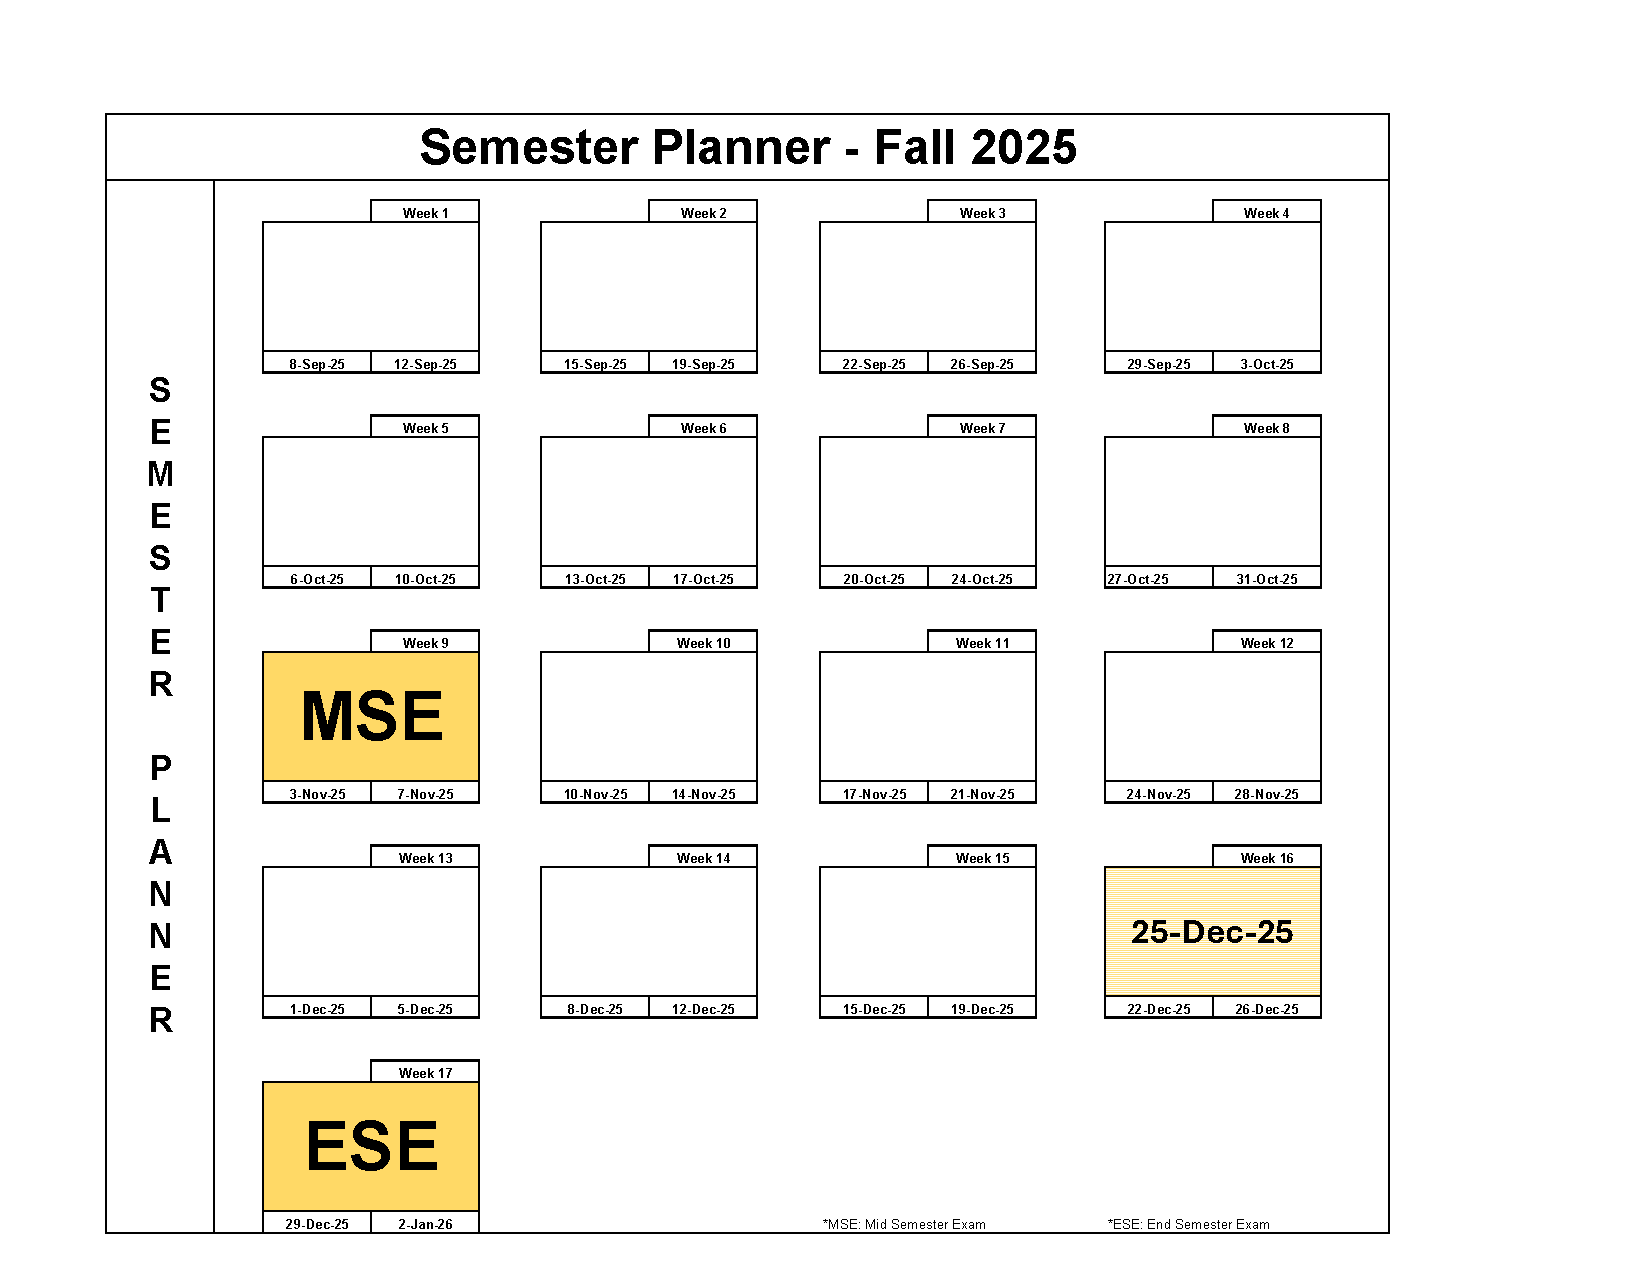
\includepdf[
  pages={1},
  scale=0.90,
  offset=0 -1.2cm,
  pagecommand={\thispagestyle{plain}\noindent{\Large\bfseries\thesection\quad Program Planning}}
]{appendices/criterion_8/I2.pdf}

\includepdf[
  pages={2-},
  pagecommand={\thispagestyle{plain}}
]{appendices/criterion_8/I2.pdf}

\refstepcounter{section}
\phantomsection
\label{annex:corrective}
\addcontentsline{toc}{section}{\protect\numberline{\thesection}Corrective Action Form}
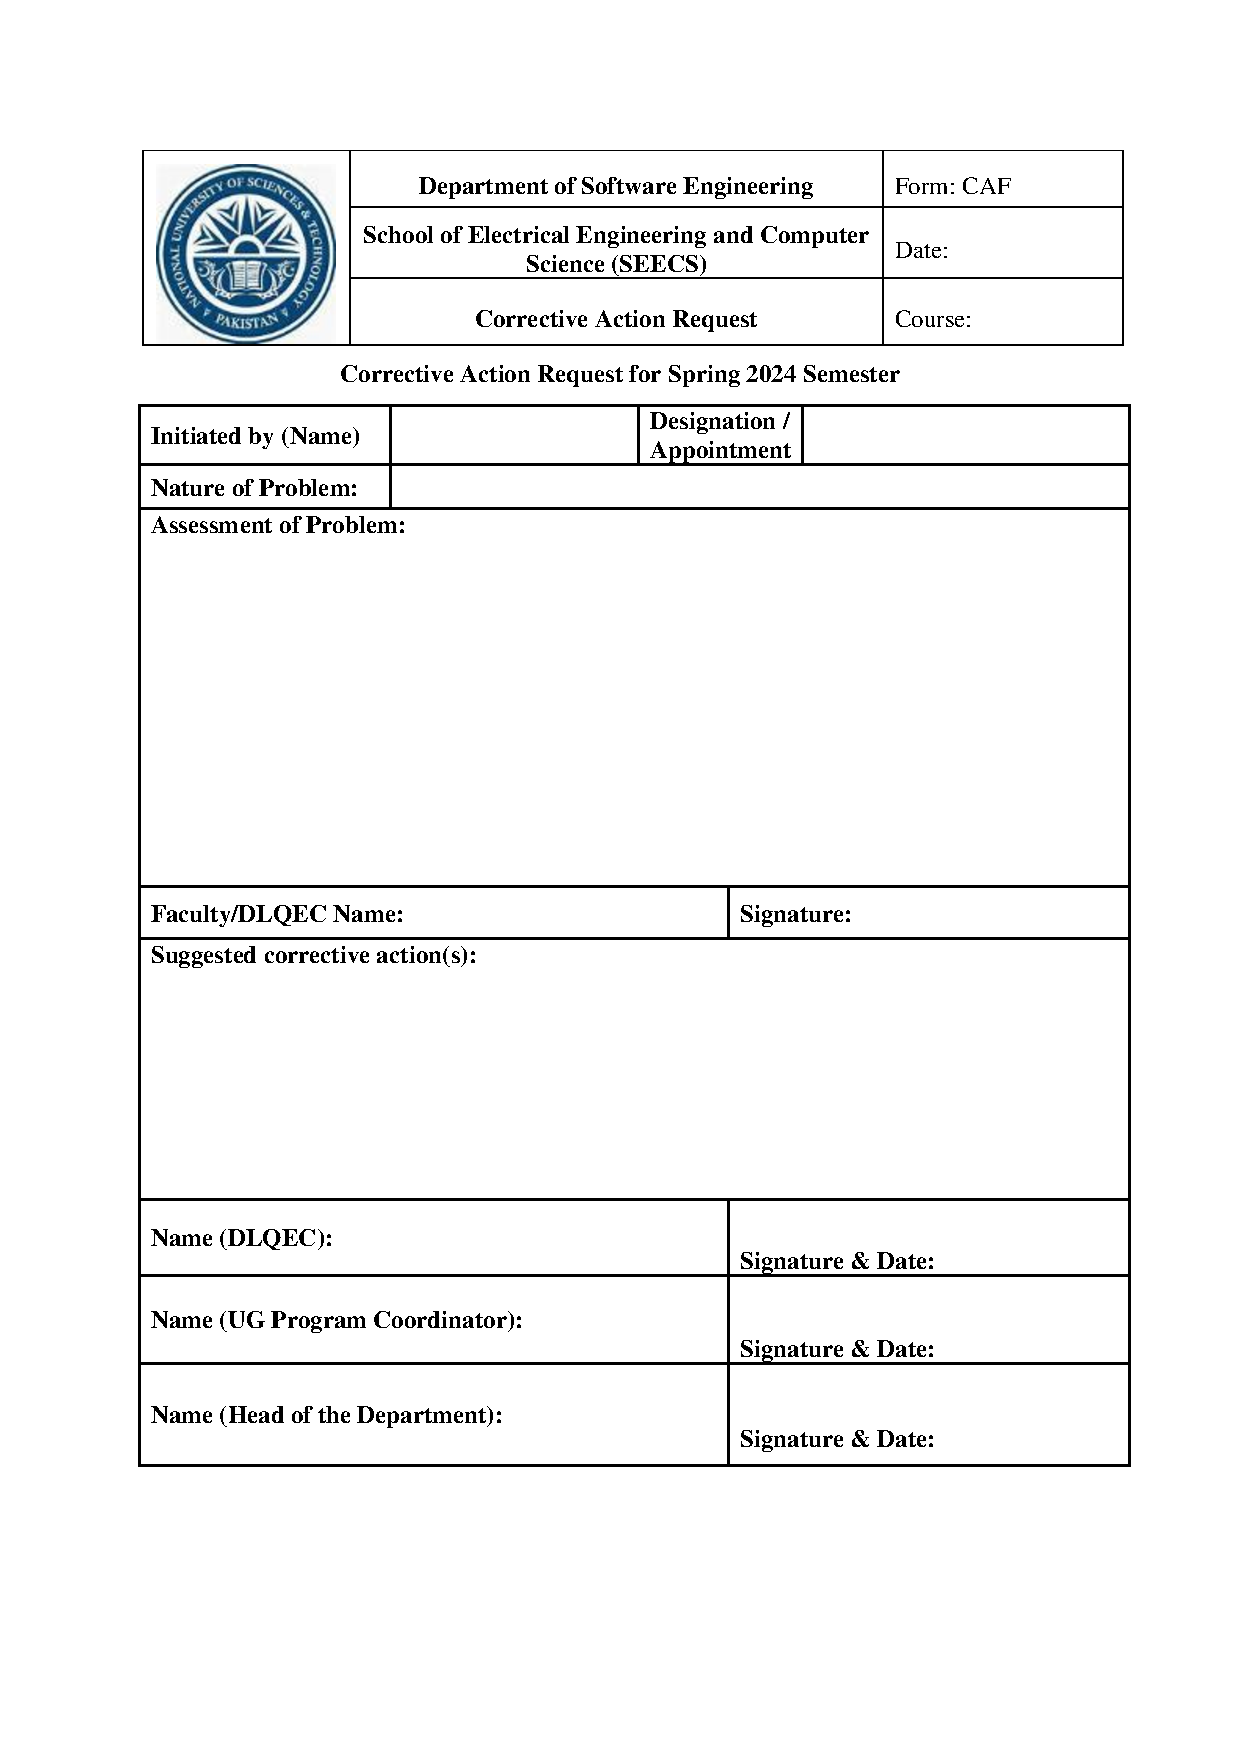
\includepdf[
  pages={1},
  scale=0.90,
  offset=0 -1.2cm,
  pagecommand={\thispagestyle{plain}\noindent{\Large\bfseries\thesection\quad Corrective Action Form}}
]{appendices/criterion_8/I3.pdf}

\refstepcounter{section}
\phantomsection
\label{annex:wp2024}
\addcontentsline{toc}{section}{\protect\numberline{\thesection}Working Paper for Curriculum Revision 2024}
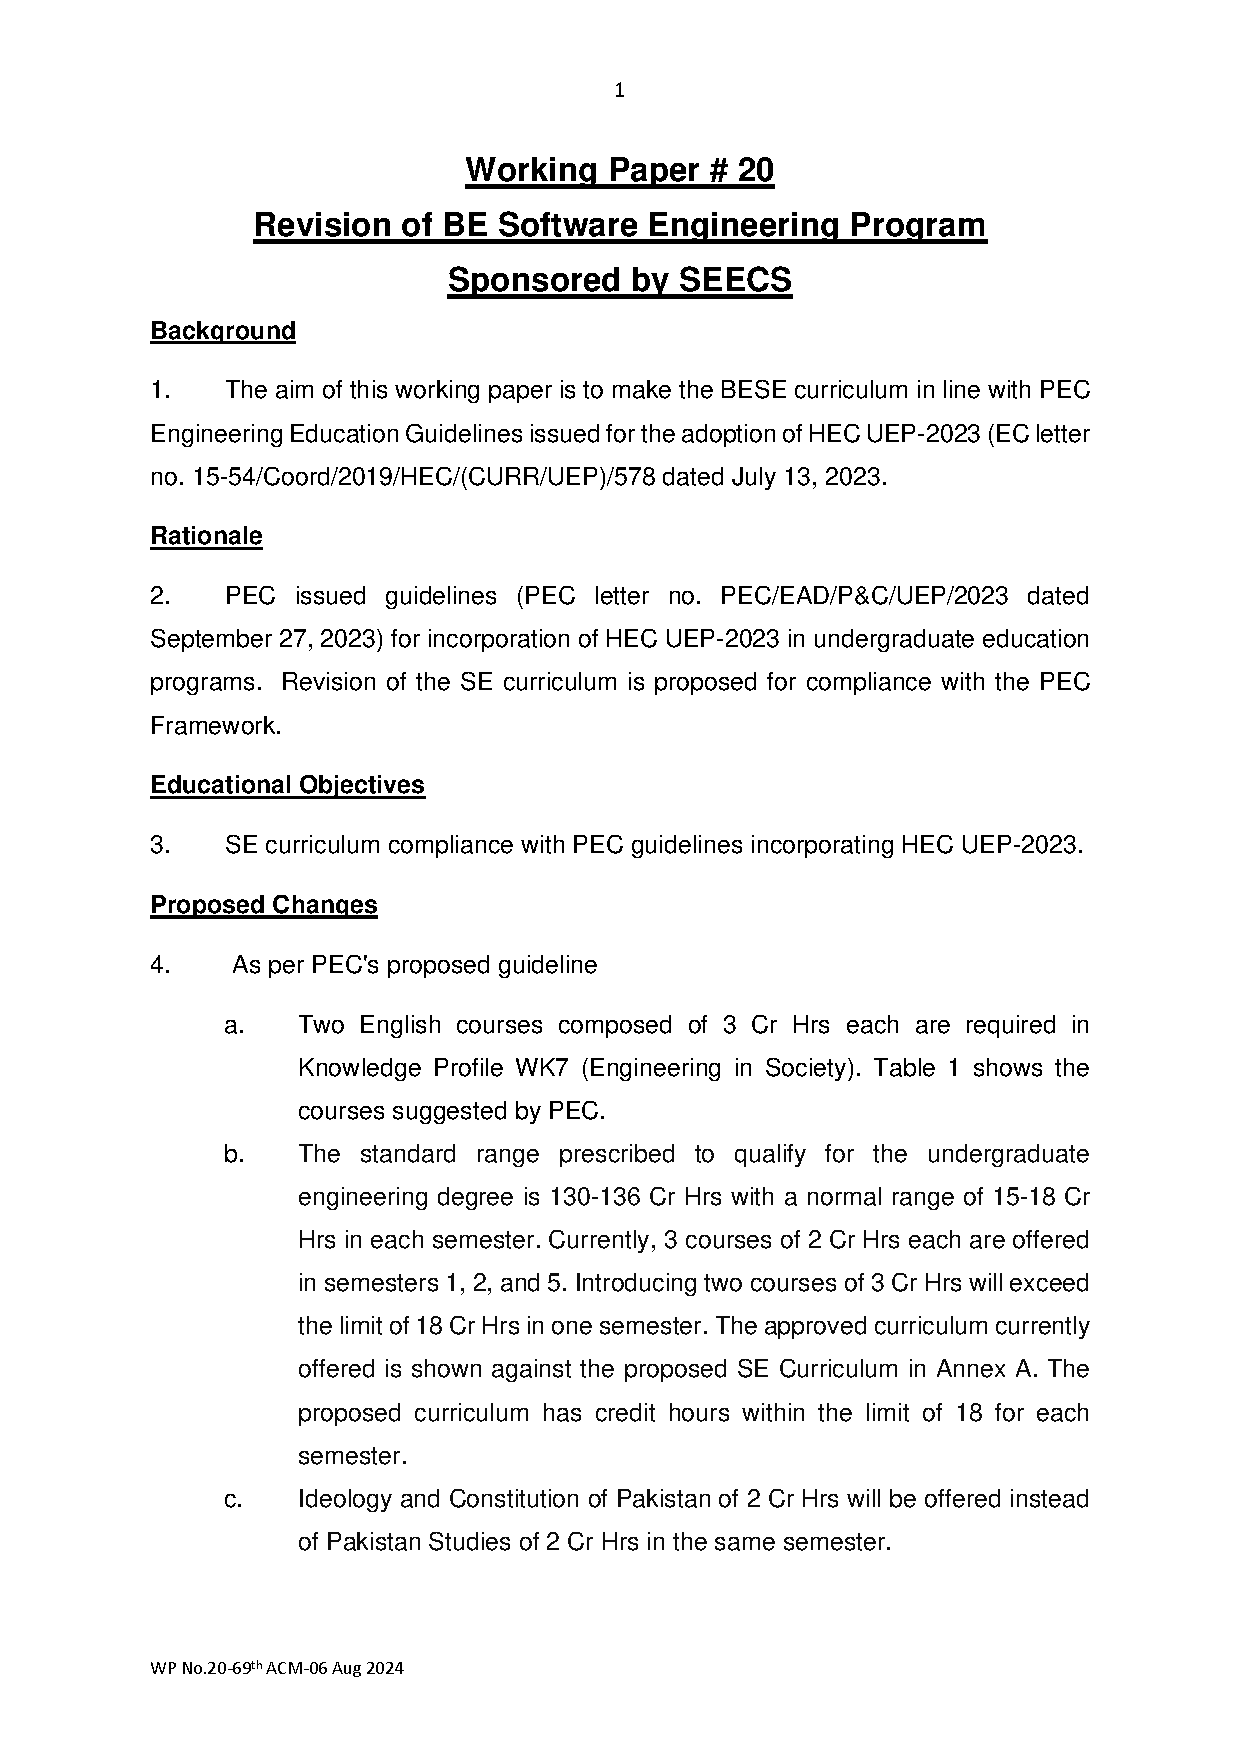
\includepdf[
  pages={1},
  scale=0.90,
  offset=0 -1.2cm,
  pagecommand={\thispagestyle{plain}\noindent{\Large\bfseries\thesection\quad Working Paper for Curriculum Revision 2024}}
]{appendices/criterion_3/Annex-2-WP-20-69-ACM-1-6.pdf}

\includepdf[
  pages={2-},
  pagecommand={\thispagestyle{plain}}
]{appendices/criterion_3/Annex-2-WP-20-69-ACM-1-6.pdf}

\refstepcounter{section}
\phantomsection
\label{annex:wp2025}
\addcontentsline{toc}{section}{\protect\numberline{\thesection}Working Paper for Curriculum Revision 2025}

\includepdf[
  pages={1},
  scale=0.90,
  offset=0 -1.2cm,
  pagecommand={\thispagestyle{plain}\noindent{\Large\bfseries\thesection\quad Working Paper for Curriculum Revision 2025}}
]{appendices/criterion_3/Annex-1-WP-30-72-ACM.pdf}


\includepdf[
  pages={2-},
  pagecommand={\thispagestyle{plain}}
]{appendices/criterion_3/Annex-1-WP-30-72-ACM.pdf}


\refstepcounter{section}
\phantomsection
\label{annex:alumni}
\addcontentsline{toc}{section}{\protect\numberline{\thesection}Alumni Survey Form}
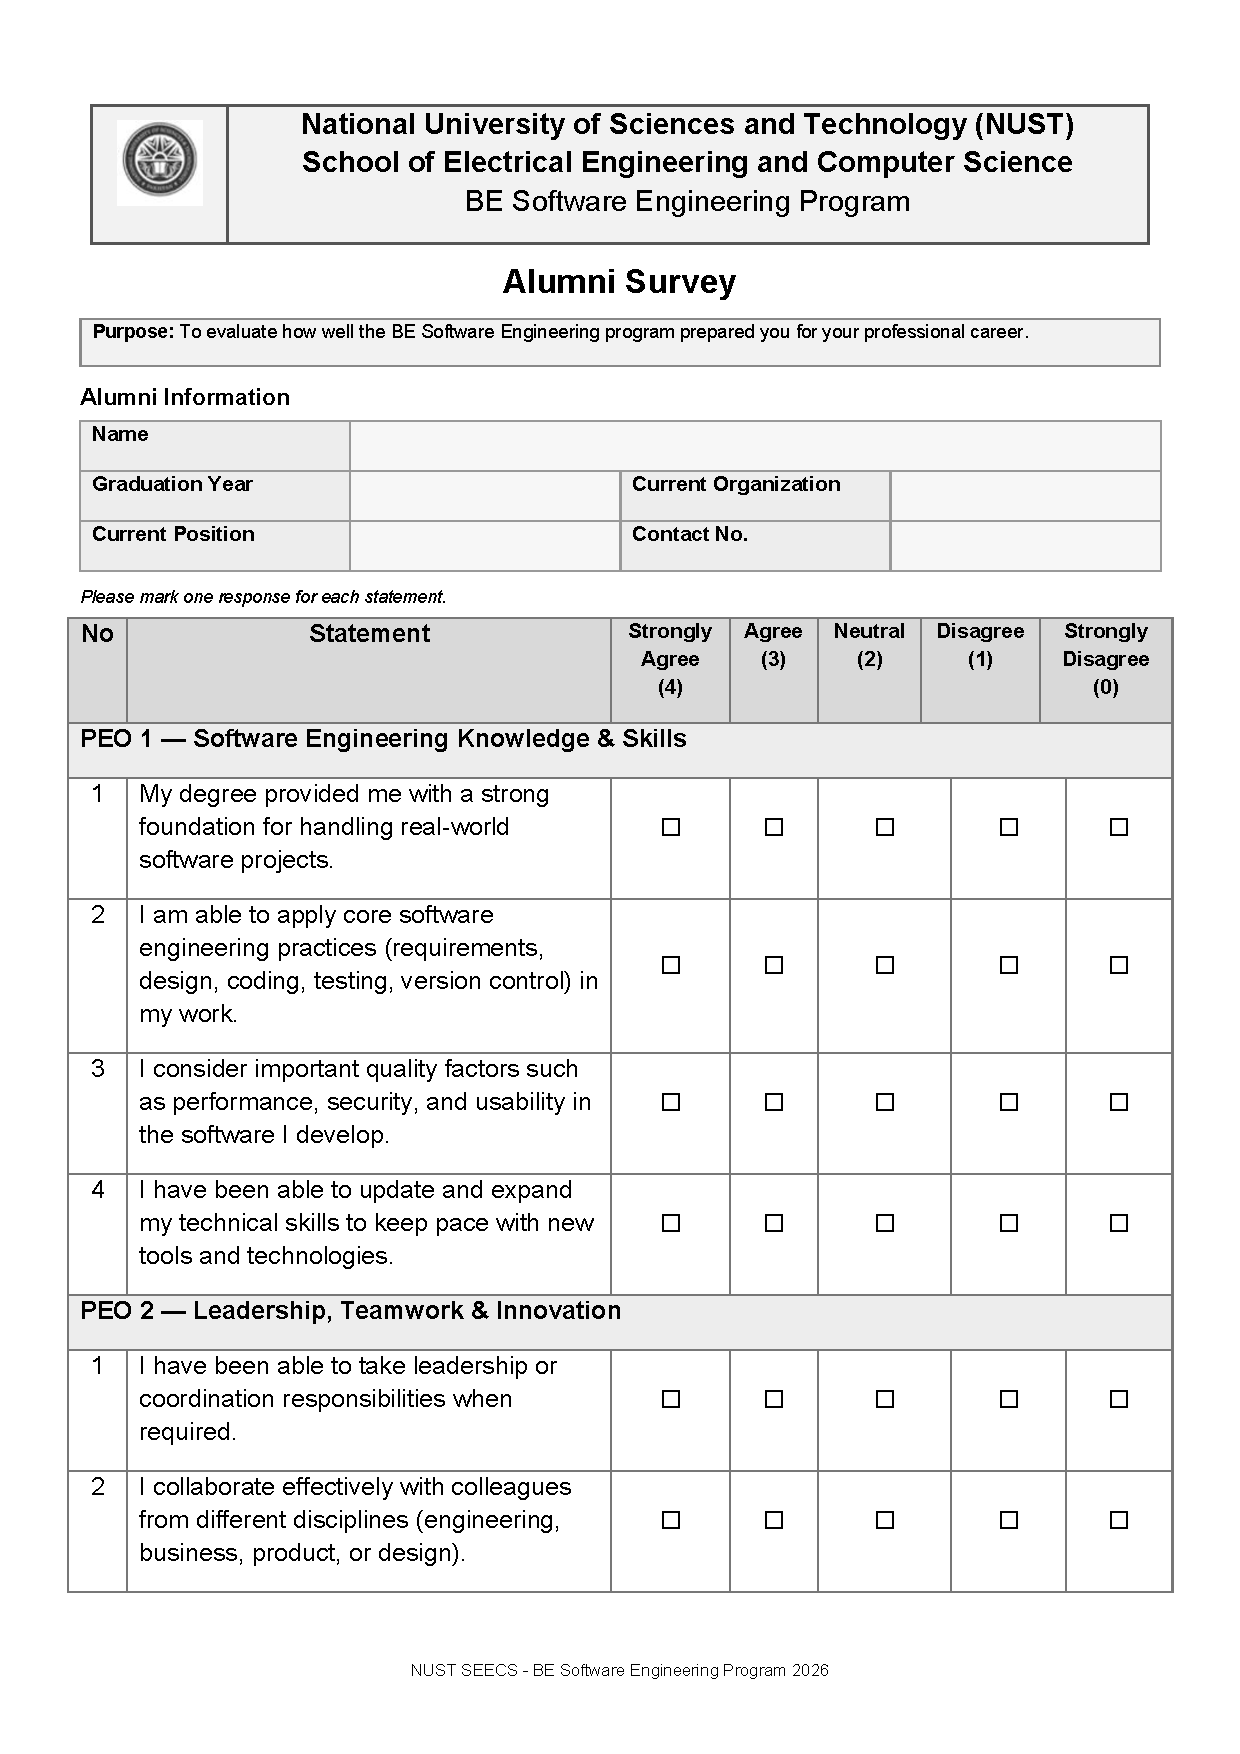
\includepdf[
  pages={1},
  scale=0.90,
  offset=0 -1.2cm,
  pagecommand={\thispagestyle{plain}\noindent{\Large\bfseries\thesection\quad Alumni Survey Form}}
]{appendices/criterion_1/Alumni Survey 2026.pdf}

\includepdf[
  pages={2-},
  pagecommand={\thispagestyle{plain}}
]{appendices/criterion_1/Alumni Survey 2026.pdf}


\refstepcounter{section}
\phantomsection
\label{annex:employer}
\addcontentsline{toc}{section}{\protect\numberline{\thesection}Employer Survey Form}
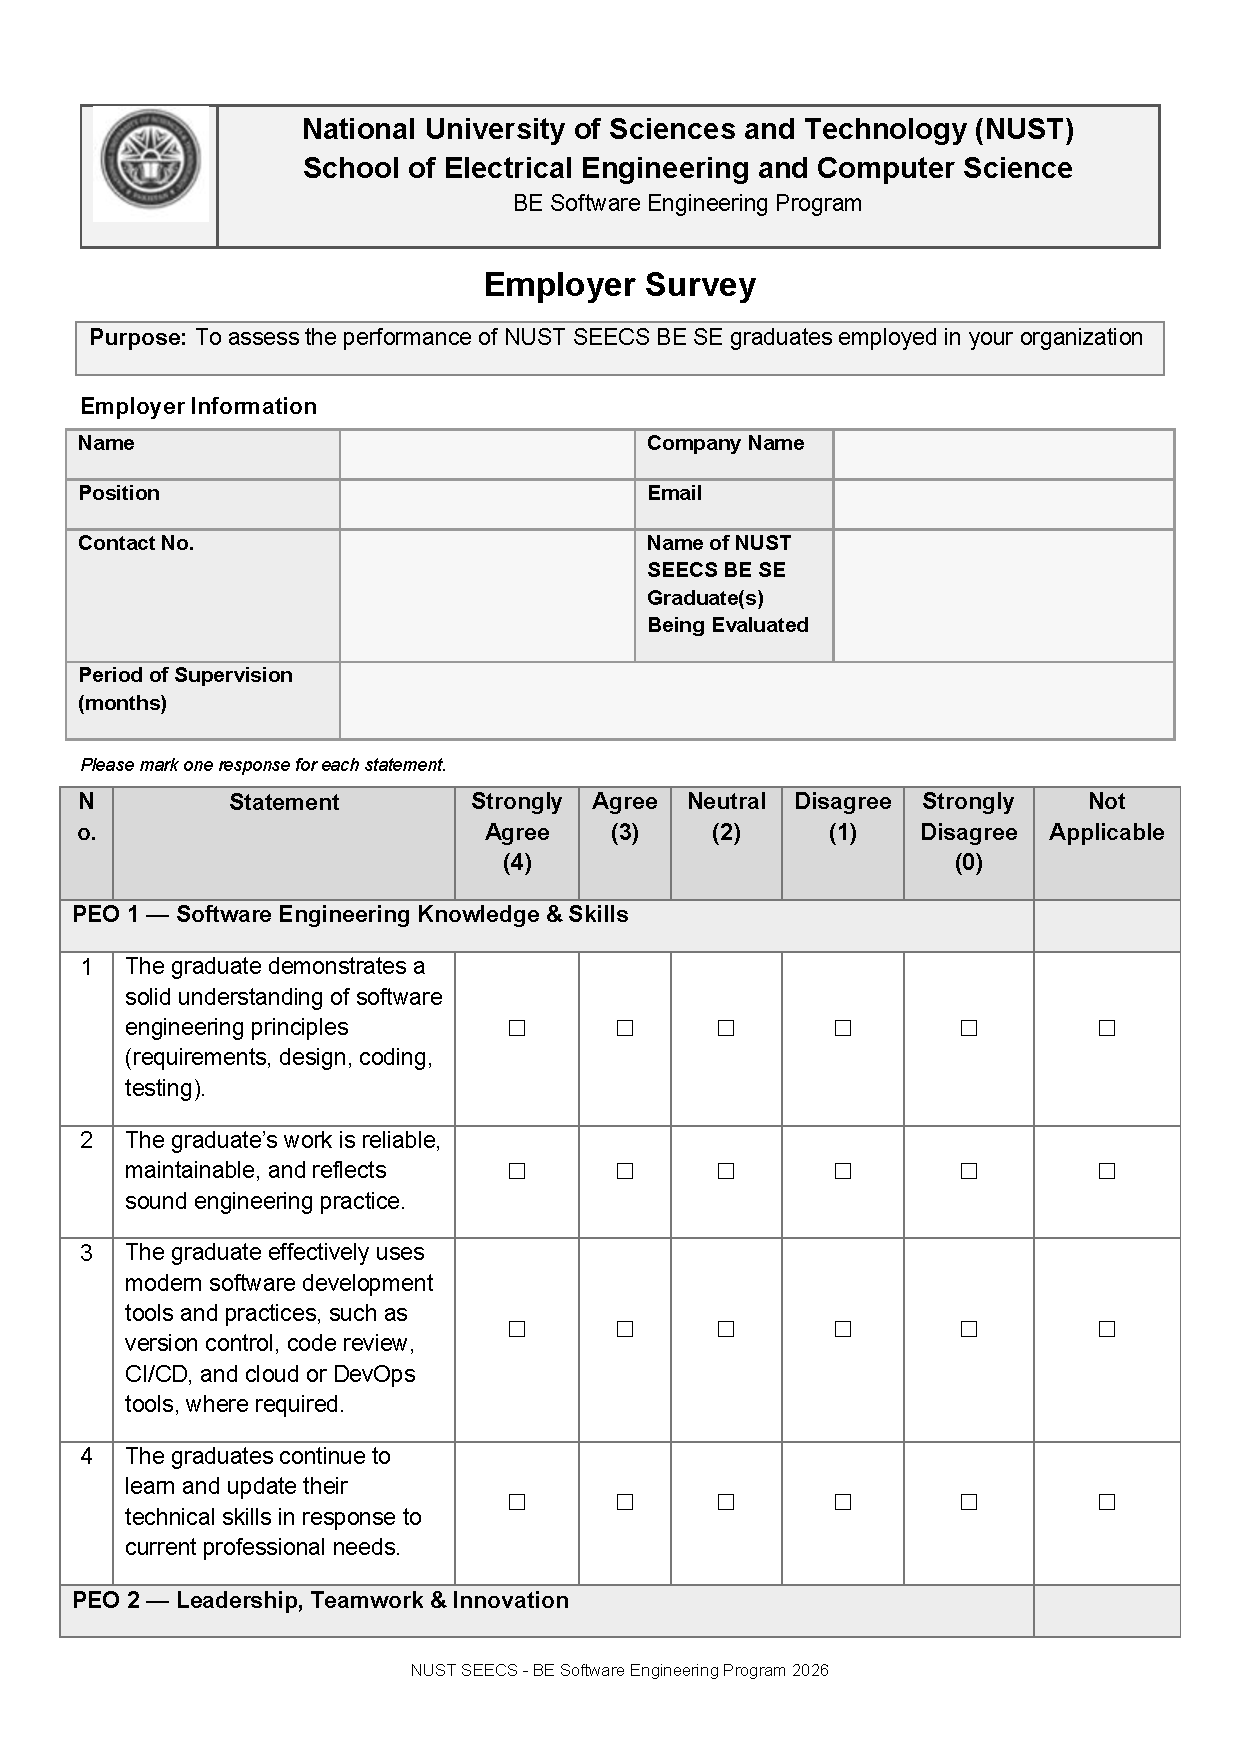
\includepdf[
  pages={1},
  scale=0.90,
  offset=0 -1.2cm,
  pagecommand={\thispagestyle{plain}\noindent{\Large\bfseries\thesection\quad Employer Survey Form}}
]{appendices/criterion_1/Employer Survey 2026.pdf}

\includepdf[
  pages={2-},
  pagecommand={\thispagestyle{plain}}
]{appendices/criterion_1/Employer Survey 2026.pdf}

\refstepcounter{section}
\phantomsection
\label{annex:advice}
\addcontentsline{toc}{section}{\protect\numberline{\thesection}Letter of Advice}
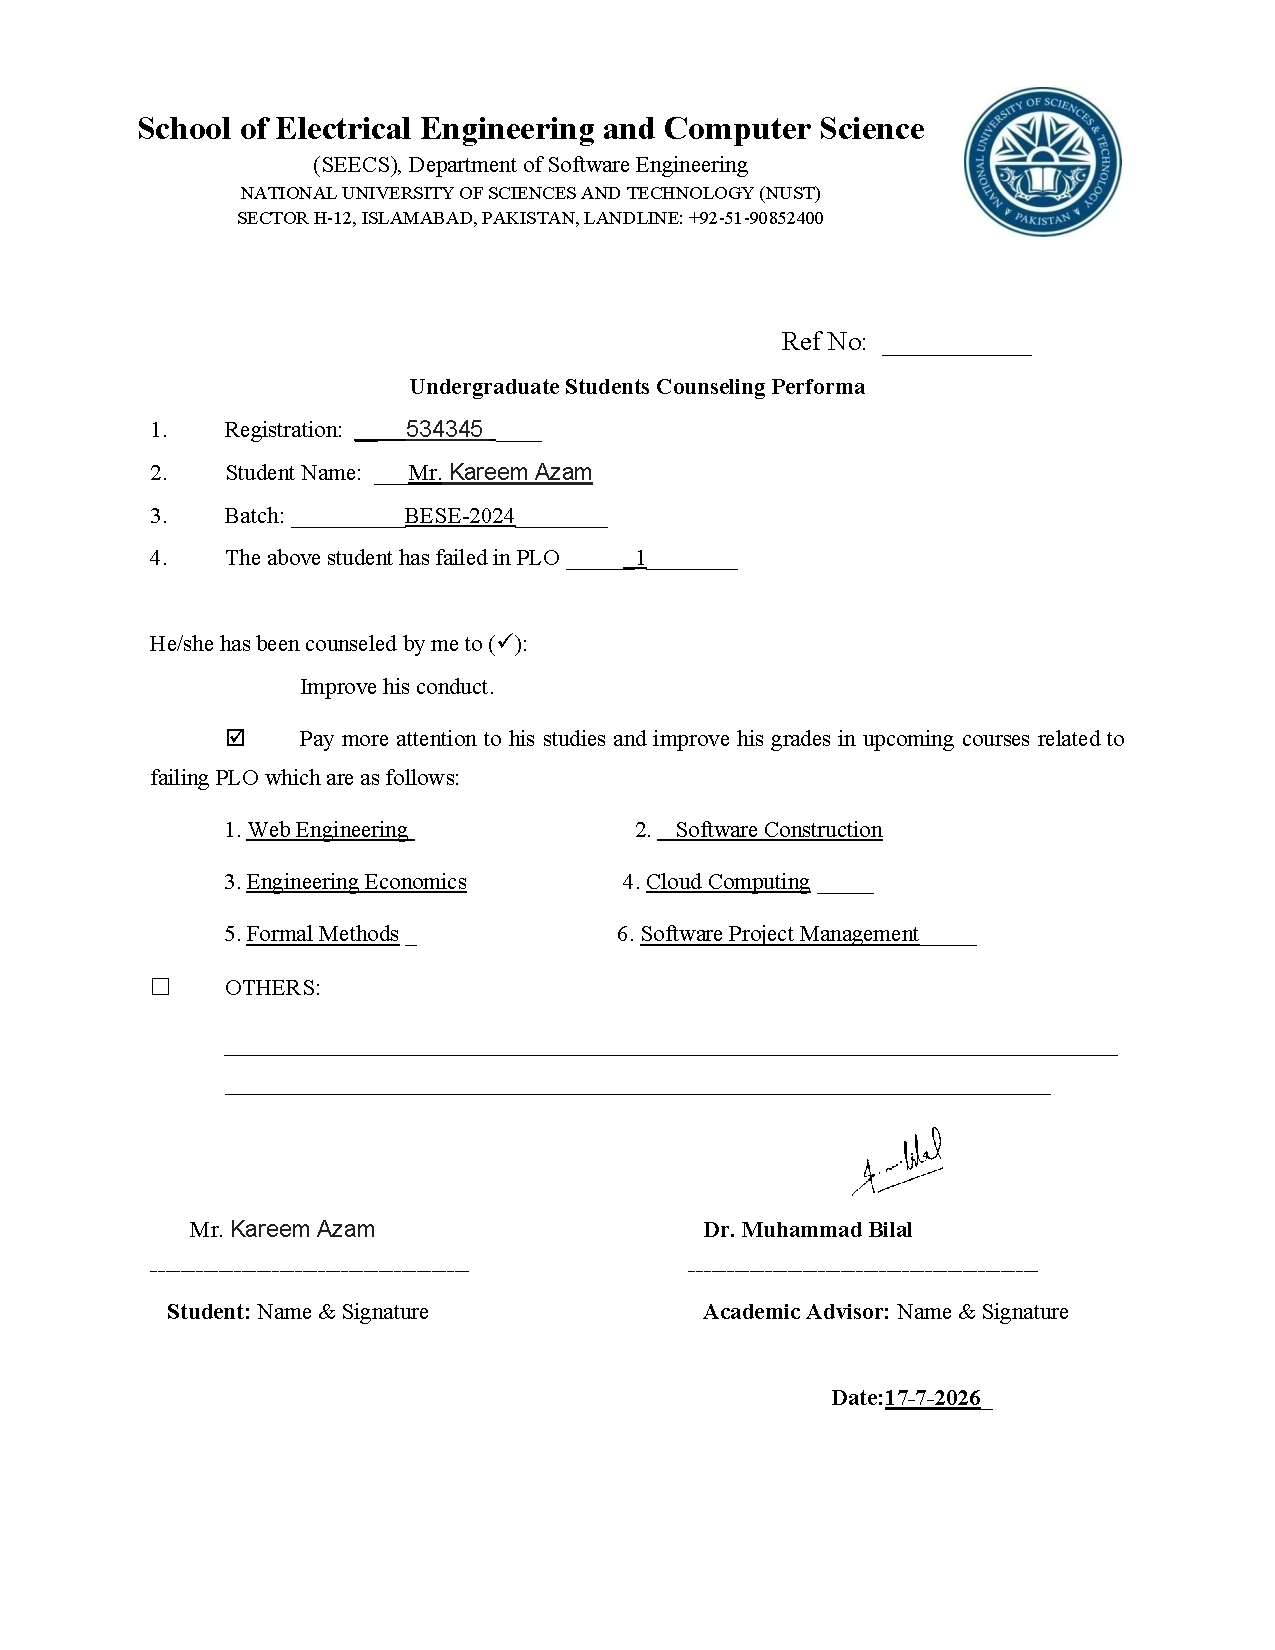
\includepdf[
  pages={1},
  scale=0.90,
  offset=0 -1.2cm,
  pagecommand={\thispagestyle{plain}\noindent{\Large\bfseries\thesection\quad Letter of Advice}}
]{appendices/criterion_8/I7.pdf}


\refstepcounter{section}
\phantomsection
\label{annex:oop}
\addcontentsline{toc}{section}{\protect\numberline{\thesection}CQI Form Sample}
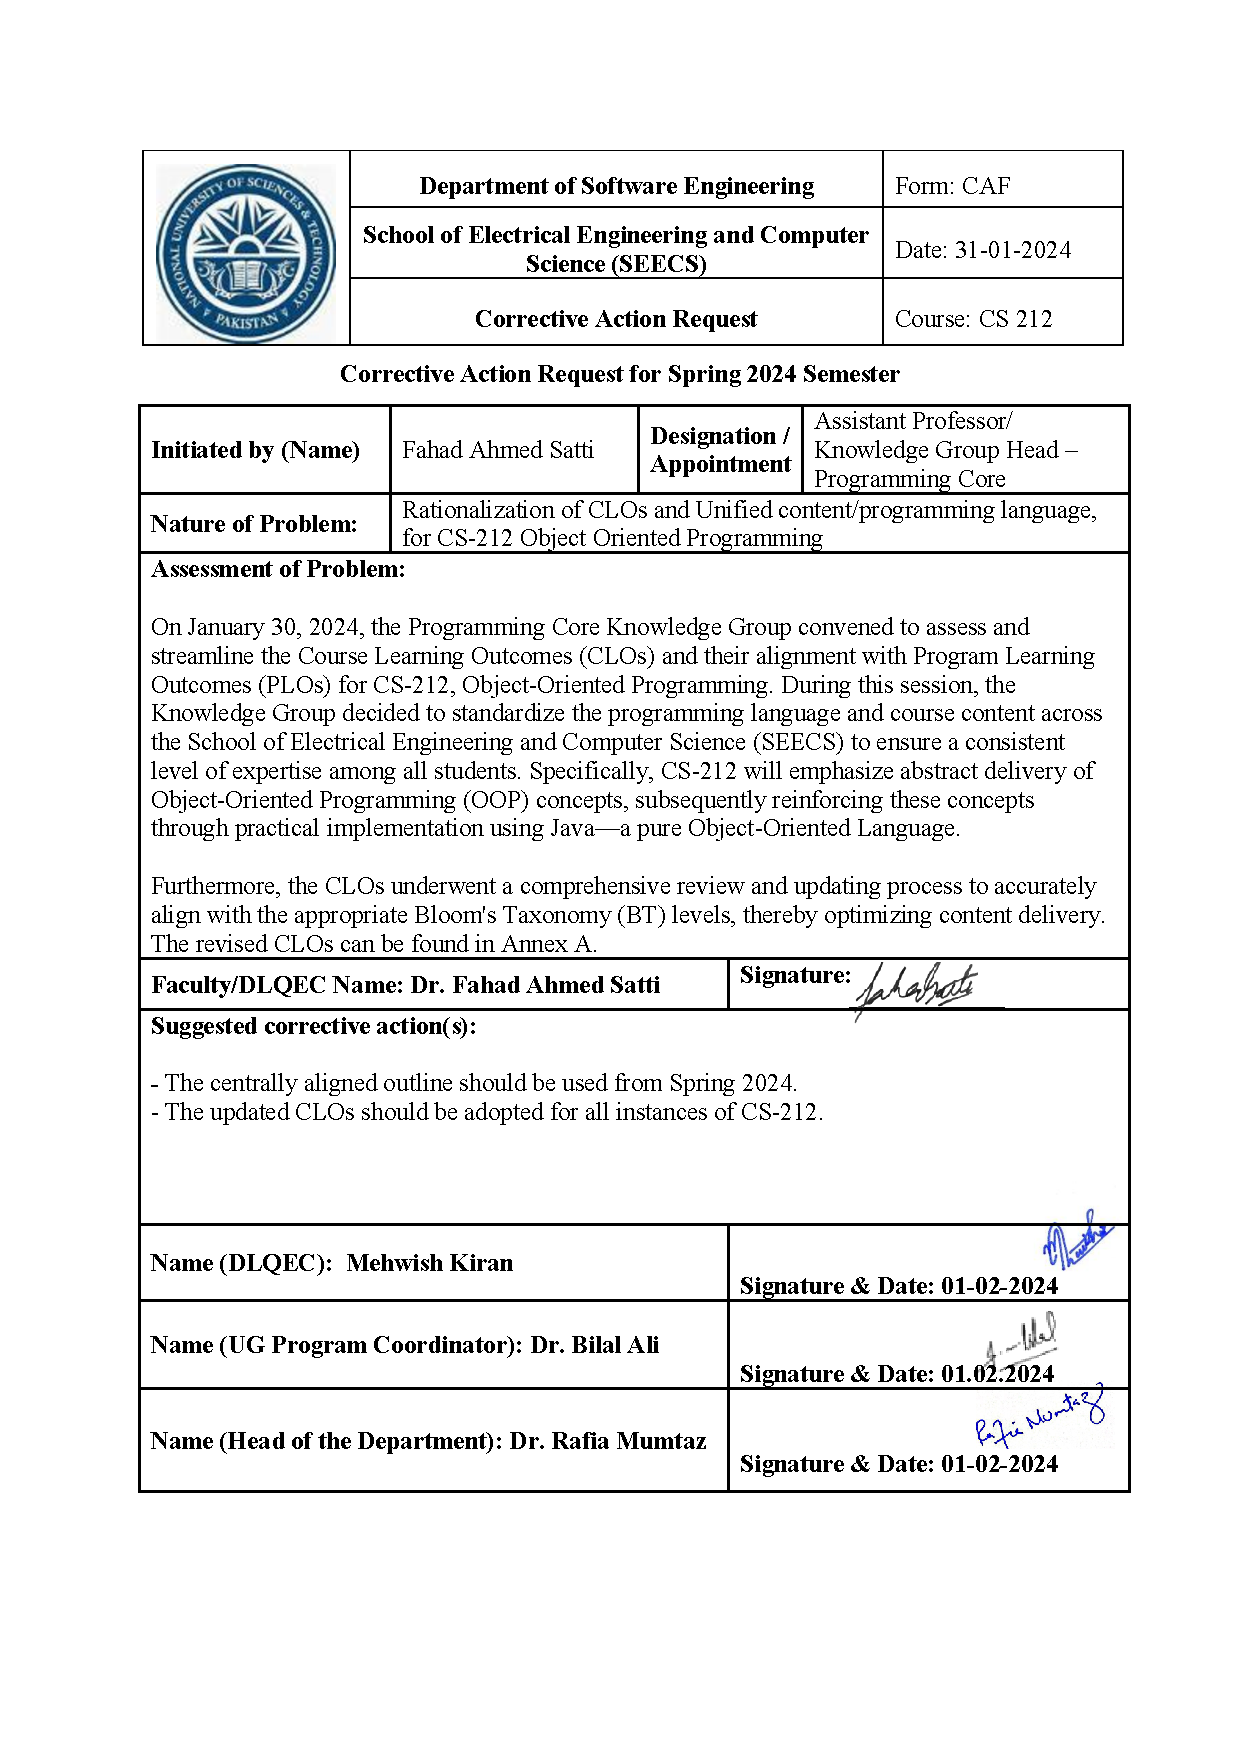
\includepdf[
  pages={1},
  scale=0.90,
  offset=0 -1.2cm,
  pagecommand={\thispagestyle{plain}\noindent{\Large\bfseries\thesection\quad CQI Form Sample}}
]{appendices/criterion_8/I8.pdf}

\includepdf[
  pages={2-},
  pagecommand={\thispagestyle{plain}}
]{appendices/criterion_8/I8.pdf}

\clearpage
\clearpage
\setcounter{section}{0}
\renewcommand{\thesection}{I.\arabic{section}}
\renewcommand{\theHsection}{annexI.\arabic{section}}

\phantomsection
\addcontentsline{toc}{chapter}{Annexure I: Criteria 9 Supporting Documents}
\label{app:criteria-9}

\refstepcounter{section}
\phantomsection
\label{app:post}
\addcontentsline{toc}{section}{\protect\numberline{\thesection}Faculty Industrial Placement Post Visit Report}

% ---- Heading block defined as a (long) macro, so \par is allowed ----
\newcommand{\annexIFirstPageHead}{%
  \noindent{\Huge\bfseries Annexure I: Criteria 9 Supporting Documents}\par
  \vspace{0.8em}
  \noindent Here we provide the supporting annexures required for Criterion 9: Industry Linkages.\par
  \vspace{0.8em}
  \noindent{\Large\bfseries\thesection\quad 
  Faculty Industrial Placement Post Visit Report}\par
}

% ---- Page 1: heading + shrunk PDF page ----
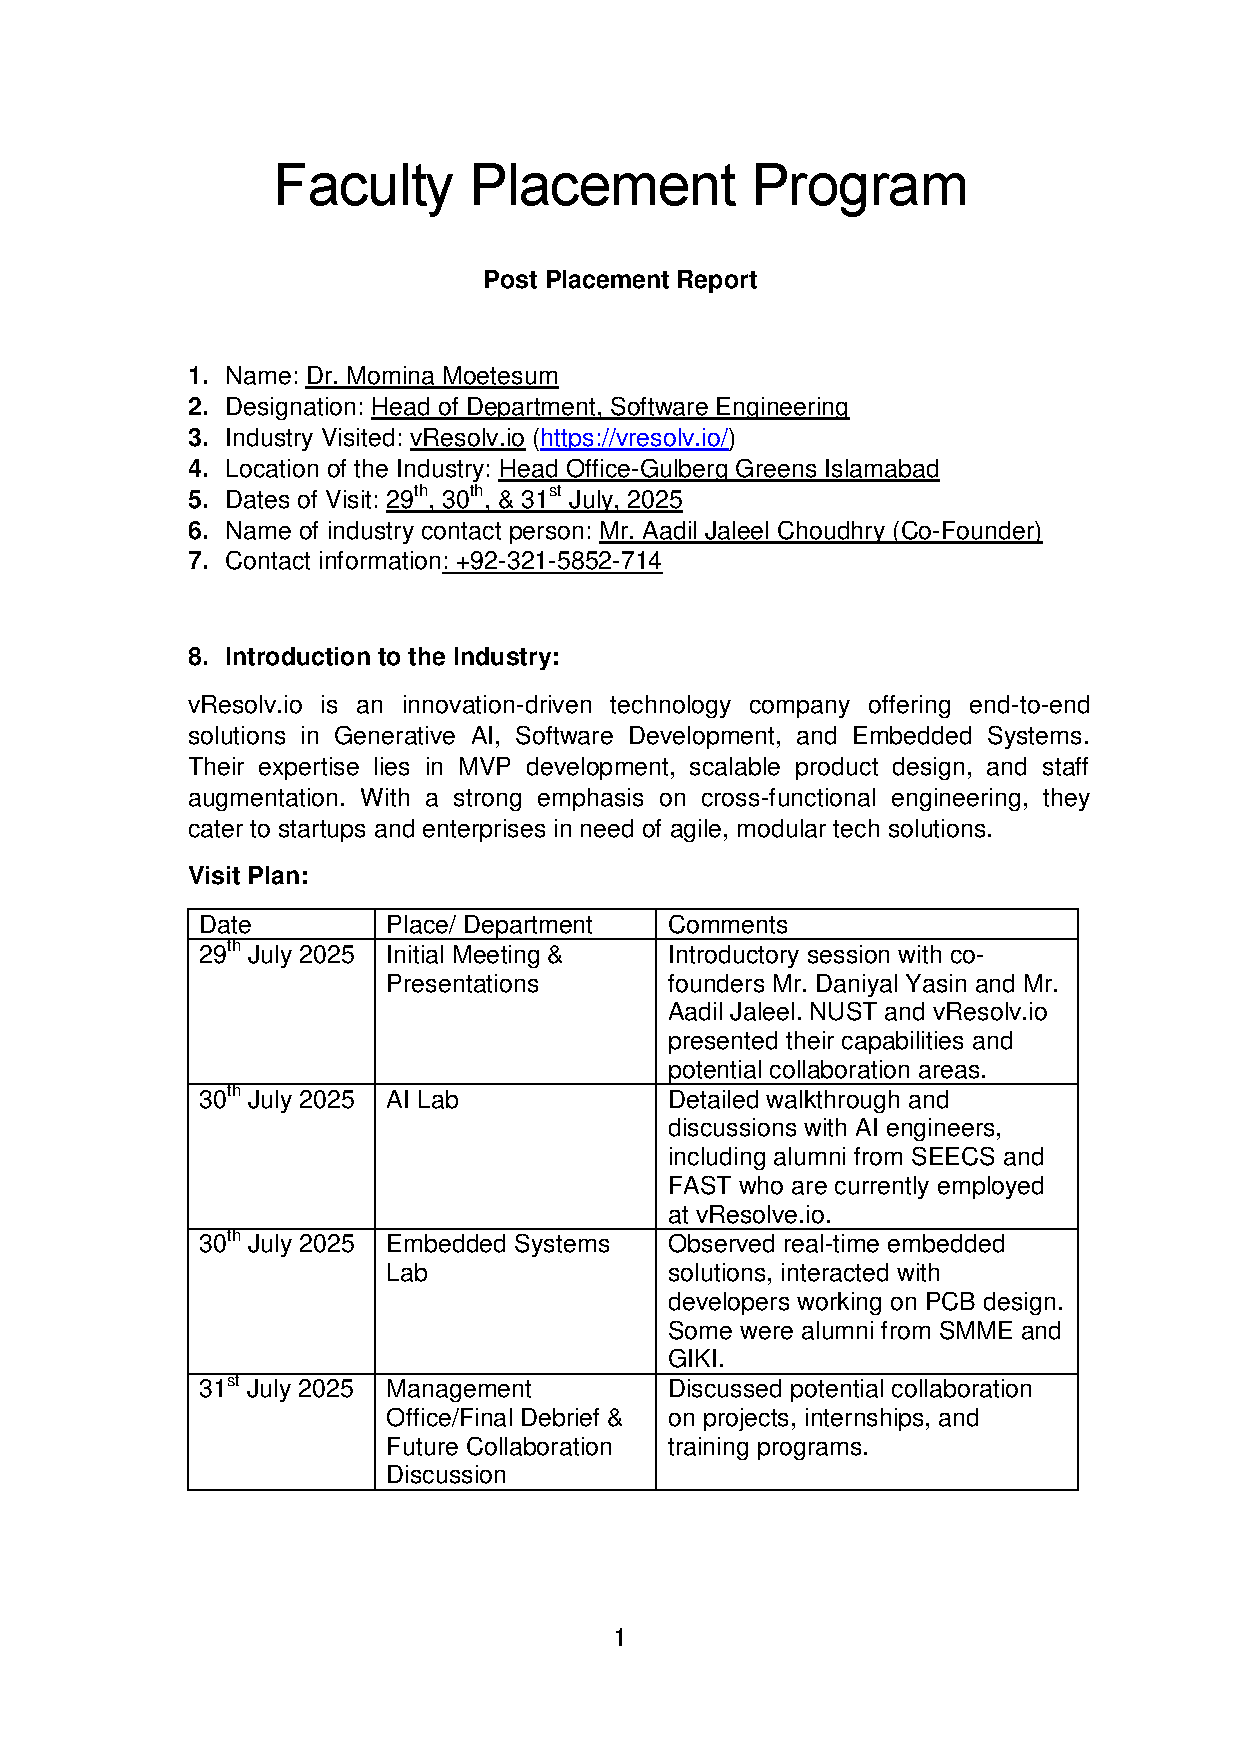
\includepdf[
  pages={1},
  scale=0.9,
  offset=0 -3.2cm,
  pagecommand={\thispagestyle{plain}\annexIFirstPageHead}
]{appendices/criterion_9/post.pdf}

% ---- Pages 2 to end: unchanged ----
\includepdf[
  pages={2-},
  pagecommand={\thispagestyle{plain}}
]{appendices/criterion_9/post.pdf}

\refstepcounter{section}
\phantomsection
\label{annex:industryproj}
\addcontentsline{toc}{section}{\protect\numberline{\thesection}Sample Industry FYDPs}
\includepdf[
  pages={1},
  scale=0.90,
  offset=0 -1.2cm,
  pagecommand={\thispagestyle{plain}\noindent{\Large\bfseries\thesection\quad Sample Industry FYDPs}}
]{appendices/criterion_9/Industry_Projects.pdf}

\includepdf[
  pages={2-},
  pagecommand={\thispagestyle{plain}}
]{appendices/criterion_9/Industry_Projects.pdf}
\clearpage
%\renewcommand{\thechapter}{I\arabic{chapter}}


%\clearpage

%\input{annexures/AnnexI1}
%\input{annexures/AnnexI2}
%\input{annexures/AnnexI3}
%\input{annexures/AnnexI4}
%\input{annexures/AnnexI5}
%\input{annexures/AnnexI6}
%\input{annexures/AnnexI7}
%\input{annexures/AnnexI8}



%\input{appendices/criterion_6/Facilities_Annexures}



%\clearpage
\chapter*{Annexure C: Criteria 3 Supporting Documents}
\phantomsection
\addcontentsline{toc}{chapter}{Annexure C: Criteria 3 Supporting Documents}
\label{app:crtieria-3}



% \clearpage
% \phantomsection
% \chapter*{Annexure C: Criteria 3 Supporting Documents}
% \addcontentsline{toc}{chapter}{Annexure C: Criteria 3 Supporting Documents}
% \label{app:crtieria-3}

This section provides supporting annexures required for the Criterion 3: Curriculum and Learning Process.

% \setcounter{section}{0}
% \renewcommand{\thesection}{C.\arabic{section}}

\setcounter{section}{0}
\renewcommand{\thesection}{C.\arabic{section}}
\renewcommand{\theHsection}{annexC.\arabic{section}}


\phantomsection
\section{Intake 2K25 WP No. 30, 72nd ACM}
\label{app:criteria3-intake-2k25-wp30}
The BE Software Engineering (BESE) curriculum at SEECS, NUST, was revised to align the program with the Pakistan Engineering Council (PEC) Engineering Education Guidelines for implementing the Higher Education Commission’s Undergraduate Education Policy (UEP-2024). The revision responds to the mandatory inclusion of specified general education courses in undergraduate engineering programs from Fall 2025 and aims to maintain compliance with the updated credit-hour requirements while preserving the sequence of core Software Engineering courses.

The revised curriculum introduces Fehm-e-Quran-I (1 credit hour) in the first semester and Fehm-e-Quran-II (1 credit hour) in the second semester. Applications of ICT (2+1 credit hours) is also introduced in the first semester. In addition, Pakistan Studies (2 credit hours) is reintroduced as a compulsory course in the fourth semester, replacing the earlier arrangement in which Ideology and Constitution of Pakistan was offered in the first semester. These changes address the prescribed general education requirements under HEC UEP-2024 and the PEC framework.

To maintain an appropriate distribution of credit hours, several existing courses have been relocated between semesters. Occupational Health and Safety and Sociology Elective-II have been moved to the eighth semester, while Expository Writing and Discrete Mathematics have been repositioned within the curriculum. Selected mathematical courses have also been rescheduled. These adjustments help satisfy the minimum requirement of 15 credit hours per semester, where applicable, and the maximum limit of 21 credit hours, without disrupting the progression of core technical courses.

The revision also removes Engineering Drawing and Workshop Practice, which were part of the earlier common first-year engineering structure but are no longer required under the updated PEC curriculum for Software Engineering. Their removal supports compliance with the prescribed maximum of 140 credit hours and creates greater scope for domain-specific and industry-relevant learning. Furthermore, the number of core engineering elective courses has increased from five to six, with corresponding adjustments to elective credit-hour allocations. The semester-wise placement of electives remains flexible, allowing courses to be offered with different credit-hour configurations, as specified in the revised scheme.

Overall, the 2025 revision incorporates the requirements of HEC UEP-2024 and the updated PEC framework while refining course sequencing, elective provision, and credit-hour distribution. The proposal was approved by the Faculty Board of Studies (FBS) on 8 July 2025 and endorsed by the University Curriculum Review Committee (UCRC) on 28 August 2025. The revised unified BE Software program at SEECS and MCS was recommended for implementation from the Fall 2025 batch.
\includefullannexure{appendices/criterion_3/Annex-1-WP-30-72-ACM.pdf}

\clearpage
\phantomsection
\section{Intake 2K24 WP No. 20, 69th ACM}
\label{app:criteria-3_intake-2k24-wp20}

The BE Software Engineering (BESE) curriculum at SEECS, NUST, was revised to align the program with the Pakistan Engineering Council (PEC) Engineering Education Guidelines for the adoption of the Higher Education Commission’s Undergraduate Education Policy (UEP-2023). The revision was proposed in accordance with the PEC framework issued in September 2023 and recommended for implementation in the Fall 2024 intake. The primary objective was to ensure regulatory compliance while maintaining the prescribed credit-hour limits and a balanced distribution of courses across semesters. The revision introduced changes to the humanities component of the curriculum, particularly the knowledge area WK-7: Engineering in Society. In the first semester, the existing English (2 credit hours) course was replaced with Functional English (3 credit hours) to meet the revised requirements. Similarly, Communication Skills (2 credit hours) in the second semester was replaced with Expository Writing (3 credit hours). These changes strengthened the formal English and writing components in accordance with the PEC guidelines. To accommodate the increased credit hours without exceeding the prescribed semester limits, the curriculum was reorganized while retaining a maximum of 18 credit hours per semester where applicable.

The revision also updated the Pakistan-related studies requirement. Pakistan Studies (2 credit hours) in the first semester was replaced with Ideology and Constitution of Pakistan (2 credit hours). In addition, Occupational Health and Safety (1 credit hour) was moved from the first to the second semester, while Islamic Studies (2 credit hours) was shifted from the second to the fourth semester. The revised curriculum provides Ethics (2 credit hours) alongside Islamic Studies in the fourth semester for non-Muslim students, in accordance with the proposed framework. Further adjustments were made to the distribution of humanities and elective courses. Sociology Elective-I was moved from the fourth semester to the fifth semester, where it replaced Technical and Business Writing (2 credit hours), which was removed from the curriculum. These changes reorganized the non-technical course component while preserving the overall structure of the eight-semester degree program.

The revision largely retained the existing technical and core Software Engineering courses, including programming, database systems, data structures and algorithms, software design and architecture, software quality engineering, cloud computing, information security, software project management, and the final-year design project. The changes therefore focused primarily on compliance with the revised PEC requirements and the redistribution of selected humanities and supporting courses rather than a fundamental restructuring of the technical curriculum.

Overall, the revision updated the BESE curriculum to incorporate the requirements associated with HEC UEP-2023 and the PEC framework, strengthened the English and writing components, revised the Pakistan studies requirement, and improved the sequencing of selected courses. The proposal was endorsed by the University Curriculum Review Committee (UCRC) on 23 July 2024 and approved by the Faculty Board of Studies (FBS), as recorded in Working Paper No. 20 for the 69th Academic Council Meeting held on 6 August 2024. The revised curriculum was recommended for implementation in the BE Software Engineering program at SEECS and MCS from the Fall 2024 batch.

\includefullannexure{appendices/criterion_3/Annex-2-WP-20-69-ACM-1-6.pdf}

\clearpage
\phantomsection
\section{Intake 2K19 WP No. 30, 64th ACM}
\label{app:criteria-3_intake-2K19-wp30}
 The program was based on the Pakistan Engineering Council’s 2020 curriculum, which was approved in August 2021. The reason for this revision was a NUST policy change to the Final Year Project (FYP). Previously the FYP carried 3 credit hours in each of the seventh and eighth semesters, but NUST had reduced the seventh-semester load to 2 credit hours and raised the eighth-semester load to 4. This redistribution left some semesters below the minimum regular credit-hour load, so the curriculum needed small adjustments to make up the difference.

The first change is simply the FYP credit split itself: SE-498 (Final Year Project I) now carries 2 credit hours in semester 7, and SE-499 (Final Year Project II) carries 4 credit hours in semester 8. This applies to all ongoing batches, meaning the Fall 2019 intake and everything after it. The remaining changes differ depending on the intake. For the Fall 2019 and Fall 2020 batches, the paper adds a new two-credit Social Science Elective, ECO-130 (Engineering Economics), to the eighth semester. This brings that semester to 12 credit hours and the whole program to 135 credit hours, made up of 110 teaching and 25 lab hours.

For the Fall 2021 and later batches, no new course was added. Instead, two electives swap places. Engineering Elective IV (Data Warehousing and Data Mining), a 3-1 course, moves from semester 7 to semester 8, while MDEE-II (Internet of Things), a 3-0 course, moves from semester 8 to semester 7. This rebalances the workload so both semesters meet the minimum. The program total for these batches is 131 plus X credit hours, where X represents the lab component of certain electives that varies depending on the course chosen. The full revised semester-wise course lists for both groups appear in Annex I and Annex II.

On the practical side, the paper states that no extra instructors or classrooms are required. The proposal was approved by the Faculty Board of Studies on 16 November 2022 and endorsed by the University Curriculum Review Committee on 16 December 2022. The paper itself says the changes take effect from Fall 2022, while the Academics Directorate recommends implementation from Spring 2023 and asks the Academic Council to make the final decision. The stated aim is to keep the BESE program aligned with the PEC’s revised curriculum while improving the quality of final year projects in line with academic and industry needs. Everything else in the existing curriculum remains unchanged.

\includefullannexure{appendices/criterion_3/Annex-3-WP-30-64-ACM.pdf}

\clearpage
\refstepcounter{section}
\phantomsection \label{app:criteria-3_Course Outline with Knowledge Group Head's Signature}
\addcontentsline{toc}{section}{\protect\numberline{\thesection}Course Outline Vetted by Knowledge Group Head}

% ---- Page 1: shrunk, shifted down, heading above it ----
\includepdf[
  pages={1},
  scale=0.85,
  offset=0 -1.5cm,
  pagecommand={\thispagestyle{plain}%
    \noindent{\Large\bfseries\thesection\quad Course Outline Vetted by Knowledge Group Head}}
]{appendices/criterion_3/Annex-4-Course_outline_CS-251 Design and Analysis of Algorithms Spring 2026.pdf}

% ---- Pages 2 to end: unchanged, at full size ----
\includepdf[
  pages={2-},
  pagecommand={\thispagestyle{plain}}
]{appendices/criterion_3/Annex-4-Course_outline_CS-251 Design and Analysis of Algorithms Spring 2026.pdf}

\clearpage
%\section{PLO Attainment Transcript}

\refstepcounter{section}
\phantomsection 
\label{app:criteria-3_PLO Attainment Transcript}
\addcontentsline{toc}{section}{\protect\numberline{\thesection}PLO Attainment Transcript}
\begin{landscape}
% ---- Page 1: shrunk, shifted down, heading above it ----
\includepdf[
  pages=1,
    landscape,
    scale=0.80,
  pagecommand={\thispagestyle{plain}%
    \noindent{\Large\bfseries\thesection\quad PLO Attainment Transcript}}
]{appendices/criterion_3/Annex-5-PLO-Attainment-Transcript.pdf}
\end{landscape}
% ---- Pages 2 to end: unchanged, at full size ----
\includepdf[
  pages={2-},
    landscape,
  pagecommand={\thispagestyle{plain}}%
]{appendices/criterion_3/Annex-5-PLO-Attainment-Transcript.pdf}


%\clearpage
%\section{Lab Rubric Based Evaluation}
\clearpage
\refstepcounter{section}
\phantomsection 
\label{app:criteria-3_Lab Rubric Based Evaluation}
\addcontentsline{toc}{section}{\protect\numberline{\thesection}Rubric Based Lab Evaluation}
\includepdf[
  pages={1},
  scale=0.85,
  offset=0 -1.5cm,
  pagecommand={\thispagestyle{plain}%
    \noindent{\Large\bfseries\thesection\quad Rubric Based Lab Evaluation}}
]{appendices/criterion_3/Annex-6-Lab-Rubric Based Evaluation.pdf}

\includepdf[
  pages={2-},
  pagecommand={\thispagestyle{plain}}
]{appendices/criterion_3/Annex-6-Lab-Rubric Based Evaluation.pdf}

%\includefullannexure{appendices/criterion_3/Annex-6-Lab-Rubric Based Evaluation.pdf}


%\section{Sample Lab Manual}
\clearpage
\refstepcounter{section}
\phantomsection 
\label{app:criteria-3_Sample Lab Manual}
\addcontentsline{toc}{section}{\protect\numberline{\thesection}Sample Lab Manual}
\includepdf[
  pages={1},
  scale=0.85,
  offset=0 -1.5cm,
  pagecommand={\thispagestyle{plain}%
    \noindent{\Large\bfseries\thesection\quad Sample Lab Manual}}
]{appendices/criterion_3/Annex-7-Sample-Lab-Manual.pdf}

\includepdf[
  pages={2-},
  pagecommand={\thispagestyle{plain}}
]{appendices/criterion_3/Annex-7-Sample-Lab-Manual.pdf}
%\includefullannexure{appendices/criterion_3/Annex-7-Sample-Lab-Manual.pdf}

%\clearpage
%\section{Sample Open Ended Lab}
%\label{app:criteria-3_Sample Open Ended Lab}
%\includefullannexure{appendices/criterion_3/Annex-8-Solving-MuJoCo-Environment-Using-RL-(Open-Ended-Lab).pdf}
\clearpage
\refstepcounter{section}
\phantomsection 
\label{app:criteria-3_Sample Open Ended Lab}
\addcontentsline{toc}{section}{\protect\numberline{\thesection}Sample Open Ended Lab}
\includepdf[
  pages={1},
  scale=0.85,
  offset=0 -1.5cm,
  pagecommand={\thispagestyle{plain}%
    \noindent{\Large\bfseries\thesection\quad Sample Open Ended Lab}}
]{appendices/criterion_3/Annex-8-Solving-MuJoCo-Environment-Using-RL-(Open-Ended-Lab).pdf}

\includepdf[
  pages={2-},
  pagecommand={\thispagestyle{plain}}
]{appendices/criterion_3/Annex-8-Solving-MuJoCo-Environment-Using-RL-(Open-Ended-Lab).pdf}

\clearpage
%\section{System of Instruction and Examination}
%\includefullannexure{appendices/criterion_3/Annex-9-System-of-instructions-and-examination.pdf}

\refstepcounter{section}
\phantomsection 
\label{app:criteria-3_System of instruction and examination}
\addcontentsline{toc}{section}{\protect\numberline{\thesection}System of Instruction and Examination}
\includepdf[
  pages=1,
  landscape,
  scale=0.85,
  offset=1.5cm 0,
  pagecommand={\thispagestyle{plain}%
    \noindent\rotatebox{90}{\Large\bfseries\thesection\quad System of Instruction and Examination}}
]{appendices/criterion_3/Annex-9-System-of-instructions-and-examination.pdf}
    
\includepdf[
  pages=2-,
  landscape,
  pagecommand={\thispagestyle{plain}}
]{appendices/criterion_3/Annex-9-System-of-instructions-and-examination.pdf}

\clearpage
%\section{CEP Policy for BESE Program}
%\label{app:criteria-3_CEP Policy for BESE Department}
%\includefullannexure{appendices/criterion_3/Annex-10-Request-for-CEP-and-OEL-Formalization.pdf}

%\refstepcounter{section}
%\phantomsection 
%\label{app:criteria-3_CEP Policy for BESE Department}
%\addcontentsline{toc}{section}{\protect\numberline{\thesection}CEP Policy for BESE Program}
%\includepdf[
%  pages={-},
%  scale=0.85,
  %offset=0 -1.5cm,
%  pagecommand={\thispagestyle{plain}%
    %\noindent{\Large\bfseries\thesection\quad CEP Policy for BESE Program}}
%]{appendices/criterion_3/Annex-10-Request-%for-CEP-and-OEL-Formalization.pdf}

%\clearpage
%\section{CEP Policy for BESE Program}
%\label{app:criteria-3_CEP Policy for BESE Department}
%\includefullannexure{appendices/criterion_3/Annex-10-Request-for-CEP-and-OEL-Formalization.pdf}

\clearpage
%\section{CEP Example}
%\label{app:criteria-3_CEP Example}
%\includefullannexure{appendices/criterion_3/Annex-11-Sample-CEP.pdf}

\refstepcounter{section}
\phantomsection 
\label{app:criteria-3_CEP Example}
\addcontentsline{toc}{section}{\protect\numberline{\thesection}CEP Example}
\includepdf[
  pages={1},
  scale=0.85,
  %offset=0 -1.5cm,
  pagecommand={\thispagestyle{plain}%
    \noindent{\Large\bfseries\thesection\quad CEP Example}}
]{appendices/criterion_3/Annex-11-Sample-CEP.pdf}
\includepdf[
  pages=2-,
  %landscape,
  pagecommand={\thispagestyle{plain}}
]{appendices/criterion_3/Annex-11-Sample-CEP.pdf}

\clearpage
\refstepcounter{section}
\phantomsection 
\label{app:criteria-3_FYP_Guidelines}
\addcontentsline{toc}{section}{\protect\numberline{\thesection}FYP Guidelines}
\includepdf[
  pages={1},
  scale=0.85,
  %offset=0 -1.5cm,
  pagecommand={\thispagestyle{plain}%
    \noindent{\Large\bfseries\thesection\quad FYP Guidelines}}
]{appendices/criterion_3/FYDP-SoP-Policy-2026.pdf}
\includepdf[
  pages=2-,
  %landscape,
  pagecommand={\thispagestyle{plain}}
]{appendices/criterion_3/FYDP-SoP-Policy-2026.pdf}

%\section{FYP Guidelines}

%\includefullannexure{appendices/criterion_3/FYDP-SoP-Policy-2026.pdf}

\clearpage
%\section{List of FYDP BESE 2K22 Batch}

%\includefullannexure{appendices/criterion_3/Annex-13-List_FYDP_BESE_2K22.pdf}

\refstepcounter{section}
\phantomsection 
\label{app:criteria-3_List of FYDP BESE 2K22 Batch}
\addcontentsline{toc}{section}{\protect\numberline{\thesection}List of FYDP BESE 2K22 Batch}
\includepdf[
  pages=1,
  scale=0.85,
  landscape,
  offset=0 -1.5cm,
  pagecommand={\thispagestyle{plain}%
    \noindent{\Large\bfseries\thesection\quad List of FYDP BESE 2K22 Batch}}
]{appendices/criterion_3/fydp-list-2k22.pdf}
    
\includepdf[
  pages=2-,
  landscape,
  pagecommand={\thispagestyle{plain}}
]{appendices/criterion_3/fydp-list-2k22.pdf}

%\clearpage
%\section{Sample Course Outline}
%\label{BSample Course Outline}
%\includefullannexure{appendices/criterion_2/CS-251 Design and Analysis of Algorithms Spring 2026.pdf}


%\clearpage
% ============================================================
\end{document}
